% Options for packages loaded elsewhere
\PassOptionsToPackage{unicode}{hyperref}
\PassOptionsToPackage{hyphens}{url}
%
\documentclass[
]{book}
\usepackage{amsmath,amssymb}
\usepackage{iftex}
\ifPDFTeX
  \usepackage[T1]{fontenc}
  \usepackage[utf8]{inputenc}
  \usepackage{textcomp} % provide euro and other symbols
\else % if luatex or xetex
  \usepackage{unicode-math} % this also loads fontspec
  \defaultfontfeatures{Scale=MatchLowercase}
  \defaultfontfeatures[\rmfamily]{Ligatures=TeX,Scale=1}
\fi
\usepackage{lmodern}
\ifPDFTeX\else
  % xetex/luatex font selection
\fi
% Use upquote if available, for straight quotes in verbatim environments
\IfFileExists{upquote.sty}{\usepackage{upquote}}{}
\IfFileExists{microtype.sty}{% use microtype if available
  \usepackage[]{microtype}
  \UseMicrotypeSet[protrusion]{basicmath} % disable protrusion for tt fonts
}{}
\makeatletter
\@ifundefined{KOMAClassName}{% if non-KOMA class
  \IfFileExists{parskip.sty}{%
    \usepackage{parskip}
  }{% else
    \setlength{\parindent}{0pt}
    \setlength{\parskip}{6pt plus 2pt minus 1pt}}
}{% if KOMA class
  \KOMAoptions{parskip=half}}
\makeatother
\usepackage{xcolor}
\usepackage{color}
\usepackage{fancyvrb}
\newcommand{\VerbBar}{|}
\newcommand{\VERB}{\Verb[commandchars=\\\{\}]}
\DefineVerbatimEnvironment{Highlighting}{Verbatim}{commandchars=\\\{\}}
% Add ',fontsize=\small' for more characters per line
\usepackage{framed}
\definecolor{shadecolor}{RGB}{248,248,248}
\newenvironment{Shaded}{\begin{snugshade}}{\end{snugshade}}
\newcommand{\AlertTok}[1]{\textcolor[rgb]{0.94,0.16,0.16}{#1}}
\newcommand{\AnnotationTok}[1]{\textcolor[rgb]{0.56,0.35,0.01}{\textbf{\textit{#1}}}}
\newcommand{\AttributeTok}[1]{\textcolor[rgb]{0.13,0.29,0.53}{#1}}
\newcommand{\BaseNTok}[1]{\textcolor[rgb]{0.00,0.00,0.81}{#1}}
\newcommand{\BuiltInTok}[1]{#1}
\newcommand{\CharTok}[1]{\textcolor[rgb]{0.31,0.60,0.02}{#1}}
\newcommand{\CommentTok}[1]{\textcolor[rgb]{0.56,0.35,0.01}{\textit{#1}}}
\newcommand{\CommentVarTok}[1]{\textcolor[rgb]{0.56,0.35,0.01}{\textbf{\textit{#1}}}}
\newcommand{\ConstantTok}[1]{\textcolor[rgb]{0.56,0.35,0.01}{#1}}
\newcommand{\ControlFlowTok}[1]{\textcolor[rgb]{0.13,0.29,0.53}{\textbf{#1}}}
\newcommand{\DataTypeTok}[1]{\textcolor[rgb]{0.13,0.29,0.53}{#1}}
\newcommand{\DecValTok}[1]{\textcolor[rgb]{0.00,0.00,0.81}{#1}}
\newcommand{\DocumentationTok}[1]{\textcolor[rgb]{0.56,0.35,0.01}{\textbf{\textit{#1}}}}
\newcommand{\ErrorTok}[1]{\textcolor[rgb]{0.64,0.00,0.00}{\textbf{#1}}}
\newcommand{\ExtensionTok}[1]{#1}
\newcommand{\FloatTok}[1]{\textcolor[rgb]{0.00,0.00,0.81}{#1}}
\newcommand{\FunctionTok}[1]{\textcolor[rgb]{0.13,0.29,0.53}{\textbf{#1}}}
\newcommand{\ImportTok}[1]{#1}
\newcommand{\InformationTok}[1]{\textcolor[rgb]{0.56,0.35,0.01}{\textbf{\textit{#1}}}}
\newcommand{\KeywordTok}[1]{\textcolor[rgb]{0.13,0.29,0.53}{\textbf{#1}}}
\newcommand{\NormalTok}[1]{#1}
\newcommand{\OperatorTok}[1]{\textcolor[rgb]{0.81,0.36,0.00}{\textbf{#1}}}
\newcommand{\OtherTok}[1]{\textcolor[rgb]{0.56,0.35,0.01}{#1}}
\newcommand{\PreprocessorTok}[1]{\textcolor[rgb]{0.56,0.35,0.01}{\textit{#1}}}
\newcommand{\RegionMarkerTok}[1]{#1}
\newcommand{\SpecialCharTok}[1]{\textcolor[rgb]{0.81,0.36,0.00}{\textbf{#1}}}
\newcommand{\SpecialStringTok}[1]{\textcolor[rgb]{0.31,0.60,0.02}{#1}}
\newcommand{\StringTok}[1]{\textcolor[rgb]{0.31,0.60,0.02}{#1}}
\newcommand{\VariableTok}[1]{\textcolor[rgb]{0.00,0.00,0.00}{#1}}
\newcommand{\VerbatimStringTok}[1]{\textcolor[rgb]{0.31,0.60,0.02}{#1}}
\newcommand{\WarningTok}[1]{\textcolor[rgb]{0.56,0.35,0.01}{\textbf{\textit{#1}}}}
\usepackage{longtable,booktabs,array}
\usepackage{calc} % for calculating minipage widths
% Correct order of tables after \paragraph or \subparagraph
\usepackage{etoolbox}
\makeatletter
\patchcmd\longtable{\par}{\if@noskipsec\mbox{}\fi\par}{}{}
\makeatother
% Allow footnotes in longtable head/foot
\IfFileExists{footnotehyper.sty}{\usepackage{footnotehyper}}{\usepackage{footnote}}
\makesavenoteenv{longtable}
\usepackage{graphicx}
\makeatletter
\def\maxwidth{\ifdim\Gin@nat@width>\linewidth\linewidth\else\Gin@nat@width\fi}
\def\maxheight{\ifdim\Gin@nat@height>\textheight\textheight\else\Gin@nat@height\fi}
\makeatother
% Scale images if necessary, so that they will not overflow the page
% margins by default, and it is still possible to overwrite the defaults
% using explicit options in \includegraphics[width, height, ...]{}
\setkeys{Gin}{width=\maxwidth,height=\maxheight,keepaspectratio}
% Set default figure placement to htbp
\makeatletter
\def\fps@figure{htbp}
\makeatother
\setlength{\emergencystretch}{3em} % prevent overfull lines
\providecommand{\tightlist}{%
  \setlength{\itemsep}{0pt}\setlength{\parskip}{0pt}}
\setcounter{secnumdepth}{5}
\usepackage{booktabs}
\ifLuaTeX
  \usepackage{selnolig}  % disable illegal ligatures
\fi
\usepackage[]{natbib}
\bibliographystyle{apalike}
\usepackage{bookmark}
\IfFileExists{xurl.sty}{\usepackage{xurl}}{} % add URL line breaks if available
\urlstyle{same}
\hypersetup{
  pdftitle={Advanced Epidemiological Analysis},
  pdfauthor={Andreas M. Neophytou and G. Brooke Anderson},
  hidelinks,
  pdfcreator={LaTeX via pandoc}}

\title{Advanced Epidemiological Analysis}
\author{Andreas M. Neophytou and G. Brooke Anderson}
\date{2024-08-18}

\begin{document}
\maketitle

{
\setcounter{tocdepth}{1}
\tableofcontents
}
\chapter{Overview}\label{overview}

This is a the coursebook for the Colorado State University course ERHS 732,
Advanced Epidemiological Analysis. This course provides the opportunity to
implement theoretical expertise through designing and conducting advanced
epidemiologic research analyses and to gain in-depth experience analyzing
datasets from the environmental epidemiology literature.

This book is in development over the Fall 2021 semester.

\section{License}\label{license}

This book is licensed under the \href{https://creativecommons.org/licenses/by-nc-sa/4.0/}{Creative Commons
Attribution-NonCommercial-ShareAlike 4.0 International
License}, while all code in
the book is under the \href{https://opensource.org/licenses/MIT}{MIT license}.

Click on the \textbf{Next} button (or navigate using the links in the table of
contents) to continue.

\chapter{Course information}\label{courseinfo}

This is a the coursebook for the Colorado State University course ERHS 732,
Advanced Epidemiological Analysis. This course provides the opportunity to
implement theoretical expertise through designing and conducting advanced
epidemiologic research analyses and to gain in-depth experience analyzing
datasets from the environmental epidemiology literature. This course will
complement the student's training in advanced epidemiological methods,
leveraging regression approaches and statistical programming, providing the
opportunity to implement their theoretical expertise through designing and
conducting advanced epidemiologic research analyses. Although basic theoretical frameworks behind analysis and statistical modeling approaches will be introduced, this course will not go into depth into statistical and epidemiologic theory and students are expected to be familiar with general epidemiologic concepts such as confounding, selection bias etc. During the course,
students will gain in-depth experience analyzing two datasets from the
environmental epidemiology literature---(1) time series data with daily measures
of weather, air pollution, and cardiorespiratory outcomes in London, England and
(2) a dataset with measures from the Framingham Heart Study. Additional datasets
and studies will be discussed and explored as a supplement.

This class will utilize a variety of instructional formats, including short lectures, readings, topic specific examples from the substantive literature, discussion and directed group work on in-course coding exercises putting lecture and discussion content into practice. A variety of teaching modalities will be used, including group discussions, student directed discussions, and in-class group exercises. It is expected that before coming to class, students will read the required papers for the week, as well as any associated code included in the papers' supplemental materials. Students should come to class prepared to do statistical programming (i.e., bring a laptop with statistical software, download any datasets needed for the week etc). Participation is based on in-class coding exercises based on each week's topic. If a student misses a class, they will be expected to complete the in-course exercise outside of class to receive credit for participation in that exercise. Students will be required to do mid-term and final projects which will be presented in class and submitted as a written write-up describing the project.

\section{Course learning objectives}\label{course-learning-objectives}

The learning objectives for this proposed course complement core epidemiology
and statistics courses required by the program and provide the opportunity for
students to implement theoretical skills and knowledge gained in those courses
in a more applied setting.

Upon successful completion of this course students will be able to:

\begin{enumerate}
\def\labelenumi{\arabic{enumi}.}
\tightlist
\item
  List several possible statistical approaches to answering an epidemiological
  research questions. (\emph{Knowledge})
\item
  Choose among analytical approaches learned in previous courses to identify
  one that is reasonable for an epidemiological research question. (\emph{Application})
\item
  Design a plan for cleaning and analyzing data to answer an epidemiological
  research question, drawing on techniques learned in previous and concurrent
  courses. (\emph{Synthesis})
\item
  Justify the methods and code used to answer an epidemiological research
  question. (\emph{Evaluation})
\item
  Explain the advantages and limitations of a chosen methodological approach
  for evaluating epidemiological data. (\emph{Evaluation})
\item
  Apply advanced epidemiological methods to analyze example data, using a
  regression modeling framework. (\emph{Application})
\item
  Apply statistical programming techniques learned in previous courses to
  prepare epidemiological data for statistical analysis and to conduct the
  analysis. (\emph{Application})
\item
  Interpret the output from statistical analyses of data for an epidemiological
  research question. (\emph{Evaluation})
\item
  Defend conclusions from their analysis. (\emph{Comprehension})
\item
  Write a report describing the methods, results, and conclusions from an
  epidemiological analysis. (\emph{Application})
\item
  Construct a reproducible document with embedded code to clean and analyze
  data to answer an epidemiological research question. (\emph{Application})
\end{enumerate}

\section{Meeting time and place}\label{meeting-time-and-place}

The class will meet on Mondays, 2:00--3:40 PM on the Colorado State University
campus in MRB 312.

\section{Class Structure and Expectations}\label{class-structure-and-expectations}

\begin{itemize}
\tightlist
\item
  \textbf{Homework/preparation:}
  It is expected that \emph{before} coming to class, students will read the required
  papers for the week, as well as the online book sections assigned for the week.
  Reading assignments will be announced the week before each class session.
  Students should come to class prepared to do statistical programming (i.e.,
  bring in a laptop with statistical software, download any datasets needed for
  the week).
\item
  \textbf{In-class schedule:}

  \begin{itemize}
  \tightlist
  \item
    Topic overview: Each class will start with a brief overview of the week's
    topic. This will focus on the material covered in that week's assigned
    reading in the online book and papers.
  \item
    Discussion of analysis and coding points: Students and faculty will be
    divided into small groups to discuss the assigned reading and think more deeply about
    the content. This is a time to bring up questions and relate the chapter
    concepts to other datasets and/or analysis methods you are familiar with.
  \item
    Group work: In small groups, students will work on designing an
    epidemiological analysis for the week's topic and developing code to
    implement that analysis. This will follow the prompts given in the assigned
    reading from the online book for the week.
  \item
    Wrap-up: We will reconvene as one group at the end to discuss topics that
    came up in small group work and to outline expectations for students before
    the next meeting.
  \end{itemize}
\end{itemize}

\section{Course grading}\label{course-grading}

\begin{tabular}{l|r}
\hline
Assessment Components & Percentage of Grade\\
\hline
Midterm written report & 30\\
\hline
Midterm presentation & 15\\
\hline
Final written report & 30\\
\hline
Final presentation & 15\\
\hline
Participation in in-course exercises & 10\\
\hline
\end{tabular}

\begin{itemize}
\tightlist
\item
  \textbf{Midterm report (written and presentation):} Students will work in groups to prepare an oral presentation and accompanying written report presenting an epidemiologic
  analysis using a time series dataset similar to the London dataset used
  for the first half of the course. The group may pick a research question
  based on the topics covered in the first half of the course. The presentation
  should be 15 minutes and should be structured like a conference presentation
  (Introduction, Methods, Results, and Discussion). The written report
  should be approximately six pages (single spaced) and should cover the
  same topics. It should include at least two (up to four) well-designed figures and / or
  tables. The written report should be created following reproducible
  research principles and using a bibliography referencing system (e.g.,
  BibTex if the student uses RMarkdown to write the report). The report
  should be written to the standard expected for a peer-reviewed
  publication in terms of clarity, grammar, spelling, and referencing.
  These Midterm reports will be due (and presented) the eighth week of class
  (seventh class session, since there will be no class for Labor Day).
\item
  \textbf{Final report (written and presentation):} Each student will prepare an oral presentation and accompanying written report presenting an epidemiologic
  analysis using either a dataset similar to the Framingham dataset used
  for the second half of the course or their own dataset from their research. The student may pick a research question
  based on the topics covered in the second half of the course. The presentation
  should be 10 minutes and should be structured like a conference presentation
  (Introduction, Methods, Results, and Discussion). The written report
  should be approximately six pages (single spaced) and should cover the
  same topics. It should include at least two well-designed figures and / or
  tables. The written report should be created following reproducible
  research principles and using a bibliography referencing system (e.g.,
  BibTex if the student uses RMarkdown to write the report). The report
  should be written to the standard expected for a peer-reviewed
  publication in terms of clarity, grammar, spelling, and referencing.
  The final presentations will be given during the assigned time period
  for finals for our course.
\item
  \textbf{Participation:} Attendance is an essential part of participating
  in the class. We understand things come up, however it is expected you
  attend every class and come prepared. Further, it is expected that you will
  actively participate in discussions and group work during the class period.
\end{itemize}

\section{Course Schedule}\label{course-schedule}

\begin{tabular}{r|l|l|l|l}
\hline
Class & Date & Study type & Topic & Book sections\\
\hline
1 & August 21 & Time series & Time series / case-crossover study designs & 3.1--3.4\\
\hline
2 & August 28 & Time series & Time series / case-crossover study designs & 3.5\\
\hline
3 & September 11 & Time series & Generalized linear models & 4.1--4.2\\
\hline
4 & September 18 & Time series & Generalized linear models & 4.3\\
\hline
5 & September 25 & Time series & Natural experiments & 5.1--5.3\\
\hline
6 & October 2 & Time series & Risk assessment & 6.1--6.3\\
\hline
7 & October 9 & Time series & Group midterm presentations & None\\
\hline
8 & October 16 & Cohort & Longitudinal cohort study designs & 7.1--7.3\\
\hline
9 & October 23 & Cohort & Longitudinal cohort study designs & 7.4\\
\hline
10 & October 30 & Cohort & Inverse probability weighting, Propensity scores & 8.1--8.3\\
\hline
11 & November 6 & Cohort & Mixed models & 9.1--9.5\\
\hline
12 & November 13 & Cohort & Instrumental variables & 10.1--10.7\\
\hline
13 & November 27 & Cohort & Discuss Final Presentation/Prepatation & None\\
\hline
14 & December 4 & Cohort & Finals presentations & None\\
\hline
15 & December 11 & Cohort & Finals presentations & None\\
\hline
\end{tabular}

\section{Textbooks and Course Materials}\label{textbooks-and-course-materials}

Readings for this course will focus on peer-reviewed literature that will be
posted for the students in the class, as well as assigned reading from this
online book.

Additional general references that will be useful
to students throughout the semester include:

\begin{itemize}
\tightlist
\item
  Garrett Grolemund and Hadley Wickham, \emph{R for Data Science}, O'Reilly, 2017. (Available for free online at \url{https://r4ds.had.co.nz/} and in print through
  most large book sellers.)
\item
  Miguel A. Hernán and James M. Robins, \emph{Causal Inference: What If}, Boca Raton: Chapman \& Hall/CRC, 2020. (Available for free online at \url{https://cdn1.sph.harvard.edu/wp-content/uploads/sites/1268/2021/01/ciwhatif_hernanrobins_31jan21.pdf} with a print version anticipated in 2021.)
\item
  Francesca Dominici and Roger D. Peng, \emph{Statistical Methods for Environmental Epidemiology with R}, Springer, 2008. (Available online through the CSU library or in print through Springer.)
\end{itemize}

\section{Prerequisites and Preparation}\label{prerequisites-and-preparation}

This course assumes experience in epidemiology and some experience
programming in statistical programming (e.g., R, SAS) and statistics.
Students should have taken (1) Epidemiologic Methods (ERHS 532/PBHL 570),
(2) Advanced Epidemiology (ERHS 640),
(3) R Programming for Research (ERHS 535) or\\
SAS and Epidemiologic Data Management (ERHS 534),
and (4) Design and Data Analysis for Researchers I (STAT 511),
or equivalent courses or experience, prior
to taking this course. While previous SAS experience is acceptable for the
course, example code will be in R, so you will find it helpful to review the basics of R
prior to class.

If you would like to prepare for this course, the best way is by reviewing
R programming, epidemiology, and regression modeling. In each chapter of the book,
we provide the required and supplemental reading for the week. If you need a review
in any of these topics, we recommend starting with the papers and book chapters
listed as general reviews of these topics in the chapters' supplemental reading
sections.

\section{Academic Honesty}\label{academic-honesty}

Lack of knowledge of the academic honesty policy is not a reasonable explanation for a violation. For more on Colorado State University's policies on \href{https://catalog.colostate.edu/general-catalog/policies/students-responsibilities/\#academic-integrity}{Academic Integrity / Misconduct}.

\chapter{Time series / case-crossover studies}\label{time-series-case-crossover-studies}

We'll start by exploring common characteristics in time series data for
environmental epidemiology. In the first half of the class, we're
focusing on a very specific type of study---one that leverages large-scale
vital statistics data, collected at a regular time scale (e.g., daily),
combined with large-scale measurements of a climate-related exposure, with
the goal of estimating the typical relationship between the level of the
exposure and risk of a health outcome. For example, we may have daily
measurements of particulate matter pollution for a city, measured daily at a set
of Environmental Protection Agency (EPA) monitors. We want to investigate
how risk of cardiovascular mortality changes in the city from day to day
in association with these pollution levels. If we have daily counts of the
number of cardiovascular deaths in the city, we can create a statistical
model that fits the exposure-response association between particulate matter
concentration and daily risk of cardiovascular mortality. These statistical
models---and the type of data used to fit them---will be the focus of the
first part of this course.

\section{Readings}\label{readings}

The required readings for this chapter are:

\begin{itemize}
\tightlist
\item
  \citet{bhaskaran2013time} Provides an overview of time series regression
  in environmental epidemiology.
\item
  \citet{vicedo2019hands} Provides a tutorial of all the steps for a
  projecting of health impacts of temperature extremes under climate change.
  One of the steps is to fit the exposure-response association using present-day data
  (the section on ``Estimation of Exposure-Response Associations'' in the paper).
  In this chapter, we will go into details on that step, and that section of the paper
  is the only required reading for this chapter. Later in the class, we'll
  look at other steps covered in this paper. Supplemental material for this paper is
  available to download by
  clicking \url{http://links.lww.com/EDE/B504}. You will need the data in this supplement
  for the exercises for class.
\end{itemize}

The following are supplemental readings (i.e., not required, but may be of
interest) associated with the material in this chapter:

\begin{itemize}
\tightlist
\item
  \citet{armstrong2012commentary} Commentary that provides context on how epidemiological
  research on temperature and health can help inform climate change policy.
\item
  \citet{dominici2008statistical1} Overview of study designs for studying climate-related
  exposures (air pollution in this case) and human health. Chapter in a book that is
  available online through the CSU library.
\item
  \citet{armstrong2006models} Covers similar material as \citet{bhaskaran2013time}, but with
  more focus on the statistical modeling framework
\item
  \citet{gasparrini2010time} Describes some of the advances made to time series study
  designs and statistical analysis, specifically in the context of temperature
\item
  \citet{basu2005temperature} Compares time series and case-crossover study designs in
  the context of exploring temperature and health. Includes a nice illustration
  of different referent periods, including time-stratified.
\item
  \citet{armstrong2014conditional} This paper describes different data structures for
  case-crossover data, as well as how conditional Poisson regression can be used
  in some cases to fit a statistical model to these data.
  Supplemental material for this paper is available at
  \url{https://bmcmedresmethodol.biomedcentral.com/articles/10.1186/1471-2288-14-122\#Sec13}.
\item
  \citet{imai2015time} Typically, the time series study design covered in this
  chapter is used to study non-communicable health outcomes. This paper discusses
  opportunities and limitations in applying a similar framework for infectious
  disease.
\item
  \citet{dominici2008statistical4} Heavier on statistics. Describes some of the
  statistical challenges of working with time series data for air pollution
  epidemiology. Chapter in a book that is available online through the CSU library.
\item
  \citet{lu2007equivalence} Heavier on statistics. This paper shows how, under
  conditions often common for environmental epidemiology studies, case-crossover
  and time series methods are equivalent.
\item
  \citet{gasparrini2014modeling} Heavier on statistics. This provides the statistical
  framework for the distributed lag model for environmental epidemiology time
  series studies.
\item
  \citet{dunn2018generalized1} Introduction to statistical models, moving into regression models and
  generalized linear models. Chapter in a book that is available online through the CSU library.
\item
  \citet{james2013introduction3} General overview of linear regression, with an R coding
  ``lab'' at the end to provide coding examples. Covers model fit, continuous, binary,
  and categorical covariates, and interaction terms. Chapter in a book that is
  available online through the CSU library.
\end{itemize}

\section{Time series and case-crossover study designs}\label{time-series-and-case-crossover-study-designs}

In the first half of this course, we'll take a deep look at how researchers
can study how environmental exposures and health risk are linked using
\emph{time series studies}. Let's start by exploring the study design for this type
of study, as well as a closely linked study design, that of \emph{case-crossover
studies}.

It's important to clarify the vocabulary we're using here. We'll use the terms
\emph{time series study} and \emph{case-crossover study} to refer specifically to a type
of study common for studying air pollution and other climate-related exposures.
However, both terms have broader definitions, particularly in fields outside
environmental epidemiology. For example, a \emph{time series study} more generally
refers to a study where data is available for the same unit (e.g., a city)
for multiple time points, typically at regularly-spaced times (e.g., daily).
A variety of statistical methods have been developed to apply to gain insight
from this type of data, some of which are currently rarely used in the specific
fields of air pollution and climate epidemiology that we'll explore here. For
example, there are methods to address autocorrelation over time in
measurements---that is, that measurements taken at closer time points are likely
somewhat correlated---that we won't cover here and that you won't see applied
often in environmental epidemiology studies, but that might be the focus of
a ``Time Series'' course in a statistics or economics department.

In air pollution and climate epidemiology, time series studies typically begin
with study data collected for an aggregated area (e.g., city, county, ZIP code)
and with a daily resolution. These data are usually secondary data, originally
collected by the government or other organizations through vital statistics
or other medical records (for the health data) and networks of monitors for
the exposure data. In the next section of this chapter, we'll explore common
characteristics of these data. These data are used in a time series study to
investigate how changes in the daily level of the exposure is associated with
risk of a health outcome, focusing on the short-term period. For example, a
study might investigate how risk of respiratory hospitalization in a city
changes in relationship with the concentration of particulate matter during the
week or two following exposure. The study period for these studies is often
very long (often a decade or longer), and while single-community time series
studies can be conducted, many time series studies for environmental epidemiology
now include a large set of communities of national or international scope.

The study design essentially compares a community with itself at different time
points---asking if health risk tends to be higher on days when exposure is higher.
By comparing the community to itself, the design removes many challenges that would
come up when comparing one community to another (e.g., is respiratory hospitalization
risk higher in city A than city B because particulate matter concentrations are
typically higher in city A?). Communities differ in demographics and other factors
that influence health risk, and it can be hard to properly control for these when
exploring the role of environmental exposures. By comparison, demographics tend to
change slowly over time (at least, compared to a daily scale) within a community.

One limitation, however, is that the study design is often best-suited to study
acute effects, but more limited in studying chronic health effects. This is tied
to the design and traditional ways of statistically modeling the resulting
data. Since a community is compared with itself, the design removes challenges in
comparing across communities, but it introduces new ones in comparing across time.
Both environmental exposures and rates of health outcomes can have strong
patterns over time, both across the year (e.g., mortality rates tend to follow
a strong seasonal pattern, with higher rates in winter) and across longer periods
(e.g., over the decade or longer of a study period). These patterns must be
addressed through the statistical model fit to the time series data, and they
make it hard to disentangle chronic effects of the exposure from unrelated
temporal patterns in the exposure and outcome, and so most time series studies
will focus on the short-term (or acute) association between exposure and outcome,
typically looking at a period of at most about a month following exposure.

The term \emph{case-crossover study} is a bit more specific than \emph{time series study},
although there has been a strong movement in environmental epidemiology towards
applying a specific version of the design, and so in this field the term often
now implies this more specific version of the design. Broadly, a case-crossover
study is one in which the conditions at the time of a health outcome are compared
to conditions at other times that should otherwise (i.e., outside of the exposure
of interest) be comparable. A case-crossover study could, for example, investigate
the association between weather and car accidents by taking a set of car accidents
and investigating how weather during the car accident compared to weather in the
same location the week before.

One choice in a case-crossover study design is how to select the control time
periods. Early studies tended to use a simple method for this---for example, taking
the day before, or a day the week before, or some similar period somewhat
close to the day of the outcome. As researchers applied the study design to large
sets of data (e.g., all deaths in a community over multiple years), they noticed
that some choices could create bias in estimates. As a result, most environmental
epidemiology case-crossover studies now use a \emph{time-stratified} approach to selecting
control days. This selects a set of control days that typically include days both
before and after the day of the health outcome, and are a defined set of days
within a ``stratum'' that should be comparable in terms of temporal trends. For
daily-resolved data, this stratum typically will include all the days within
a month, year, and day of week. For example, one stratum of comparable days might
be all the Mondays in January of 2010. These stratums are created throughout the
study period, and then days are only compared to other days within their stratum
(although, fortunately, there are ways you can apply a single statistical model
to fit all the data for this approach rather than having to fit code
stratum-by-stratum over many years).

When this is applied to data at an aggregated level (e.g., city, county, or ZIP
code), it is in spirit very similar to a time series study design, in that you
are comparing a community to itself at different time points. The main
difference is that a time series study uses statistical modeling to control from
potential confounding from temporal patterns, while a case-crossover study of
this type instead controls for this potential confounding by only comparing days
that should be ``comparable'' in terms of temporal trends, for example, comparing
a day only to other days in the same month, year, and day of week. You will
often hear that case-crossover studies therefore address potential confounding
for temporal patterns ``by design'' rather than ``statistically'' (as in time series
studies). However, in practice (and as we'll explore in this class), in
environmental epidemiology, case-crossover studies often are applied to
aggregated community-level data, rather than individual-level data, with exposure
assumed to be the same for everyone in the community on a given day. Under these
assumptions, time series and case-crossover studies have been determined to
be essentially equivalent (and, in fact, can use the same study data), only with
slightly different terms used to control for temporal patterns in the statistical
model fit to the data. Several interesting papers have been written to explore
differences and similarities in these two study designs as applied in environmental
epidemiology \citep{basu2005temperature, armstrong2014conditional, lu2007equivalence}.

These types of study designs in practice use similar datasets. In earlier
presentations of the case-crossover design, these data would be set up a bit
differently for statistical modeling. More recent work, however, has clarified
how they can be modeled similarly to when using a time series study design,
allowing the data to be set up in a similar way \citep{armstrong2014conditional}.

Several excellent commentaries or reviews are available that provide more
details on these two study designs and how they have been used specifically
investigate the relationship between climate-related exposures and health \citep{bhaskaran2013time, armstrong2006models, gasparrini2010time}.
Further, these designs are just two tools in a wider collection of study designs
that can be used to explore the health effects of climate-related exposures.
\citet{dominici2008statistical1} provides a nice overview of this broader set of designs.

\section{Time series data}\label{time-series-data}

Let's explore the type of dataset that can be used for these
time series--style studies in environmental epidemiology. In the examples
in this chapter, we'll be using data that comes as part of the Supplemental
Material in one of this chapter's required readings, \citep{vicedo2019hands}.
Follow the link for the supplement for this article and then look for the
file ``lndn\_obs.csv''. This is the file we'll use as the example data in this
chapter.

These data are saved in a csv format (that is, a plain text file, with commas
used as the delimiter), and so they can be read into R using the \texttt{read\_csv}
function from the \texttt{readr} package (part of the tidyverse). For example, you can
use the following code to read in these data, assuming you have saved them in a
``data'' subdirectory of your current working directory:

\begin{Shaded}
\begin{Highlighting}[]
\FunctionTok{library}\NormalTok{(tidyverse) }\CommentTok{\# Loads all the tidyverse packages, including readr}
\NormalTok{obs }\OtherTok{\textless{}{-}} \FunctionTok{read\_csv}\NormalTok{(}\StringTok{"data/lndn\_obs.csv"}\NormalTok{)}
\NormalTok{obs}
\end{Highlighting}
\end{Shaded}

\begin{verbatim}
## # A tibble: 8,279 x 14
##    date        year month   day   doy dow     all all_0_64 all_65_74 all_75_84
##    <date>     <dbl> <dbl> <dbl> <dbl> <chr> <dbl>    <dbl>     <dbl>     <dbl>
##  1 1990-01-01  1990     1     1     1 Mon     220       38        38        82
##  2 1990-01-02  1990     1     2     2 Tue     257       50        67        87
##  3 1990-01-03  1990     1     3     3 Wed     245       39        59        86
##  4 1990-01-04  1990     1     4     4 Thu     226       41        45        77
##  5 1990-01-05  1990     1     5     5 Fri     236       45        54        85
##  6 1990-01-06  1990     1     6     6 Sat     235       48        48        84
##  7 1990-01-07  1990     1     7     7 Sun     231       38        49        96
##  8 1990-01-08  1990     1     8     8 Mon     235       46        57        76
##  9 1990-01-09  1990     1     9     9 Tue     250       48        54        96
## 10 1990-01-10  1990     1    10    10 Wed     214       44        46        62
## # i 8,269 more rows
## # i 4 more variables: all_85plus <dbl>, tmean <dbl>, tmin <dbl>, tmax <dbl>
\end{verbatim}

This example dataset shows many characteristics that are common for datasets for
time series studies in environmental epidemiology. Time series data are essentially
a sequence of data points repeatedly taken over a certain time interval (e.g., day,
week, month etc). General characteristics of time series data for environmental epidemiology studies are:

\begin{itemize}
\tightlist
\item
  Observations are given at an aggregated level. For example, instead of
  individual observations for each person in London, the \texttt{obs} data give
  counts of deaths throughout London. The level of aggregation is often determined
  by geopolitical boundaries, for example, counties or ZIP codes in the US.
\item
  Observations are given at regularly spaced time steps over a period. In the
  \texttt{obs} dataset, the time interval is day. Typically, values will be provided
  continuously over that time period, with observations for each time interval.
  Occasionally, however, the time series data may only be available for
  particular seasons (e.g., only warm season dates for an ozone study), or
  there may be some missing data on either the exposure or health outcome over
  the course of the study period.
\item
  Observations are available at the same time step (e.g., daily) for (1) the health outcome, (2) the environmental
  exposure of interest, and (3) potential time-varying confounders. In the \texttt{obs}
  dataset, the health outcome is mortality (from all causes; sometimes, the health
  outcome will focus on a specific cause of mortality or other health outcomes such
  as hospitalizations or emergency room visits). Counts are given for everyone in
  the city for each day (\texttt{all} column), as well as for specific age categories
  (\texttt{all\_0\_64} for all deaths among those up to 64 years old, and so on). The
  exposure of interest in the \texttt{obs} dataset is temperature, and three metrics of
  this are included (\texttt{tmean}, \texttt{tmin}, and \texttt{tmax}). Day of the week is one
  time-varying factor that could be a confounder, or at least help explain
  variation in the outcome (mortality). This is included through the \texttt{dow} variable
  in the \texttt{obs} data. Sometimes, you will also see a marker for holidays included
  as a potential time-varying confounder, or other exposure variables (temperature
  is a potential confounder, for example, when investigating the relationship
  between air pollution and mortality risk).
\item
  Multiple metrics of an exposure and / or multiple health outcome counts
  may be included for each time step. In the \texttt{obs} example, three metrics of
  temperature are included (minimum daily temperature, maximum daily temperature,
  and mean daily temperature). Several counts of mortality are included, providing
  information for specific age categories in the population. The different metrics
  of exposure will typically be fit in separate models, either as a sensitivity
  analysis or to explore how exposure measurement affects epidemiological results.
  If different health outcome counts are available, these can be modeled in separate
  statistical models to determine an exposure-response function for each outcome.
\end{itemize}

\section{Exploratory data analysis}\label{exploratory-data-analysis}

When working with time series data, it is helpful to start with some exploratory
data analysis. This type of time series data will often be secondary data---it is
data that was previously collected, as you are re-using it. Exploratory data analysis
is particularly important with secondary data like this. For primary data that you
collected yourself, following protocols that you designed yourself, you will often
be very familiar with the structure of the data and any quirks in it by the time
you are ready to fit a statistical model. With secondary data, however, you will
typically start with much less familiarity about the data, how it was collected, and
any potential issues with it, like missing data and outliers.

Exploratory data analysis can help you become familiar with your data. You can use
summaries and plots to explore the parameters of the data, and also to identify
trends and patterns that may be useful in designing an appropriate statistical
model. For example, you can explore how values of the health outcome are distributed,
which can help you determine what type of regression model would be appropriate, and
to see if there are potential confounders that have regular relationships with
both the health outcome and the exposure of interest. You can see how many
observations have missing data for the outcome, the exposure, or confounders of
interest, and you can see if there are any measurements that look unusual.
This can help in identifying quirks in how the data were recorded---for example,
in some cases ground-based weather monitors use -99 or -999 to represent missing
values, definitely something you want to catch and clean-up in your data
(replacing with R's \texttt{NA} for missing values) before fitting a statistical model!

The following applied exercise will take you through some of the
questions you might want to answer through this type of exploratory analysis.
In
general, the \texttt{tidyverse} suite of R packages has loads of tools for exploring and
visualizing data in R.
The \texttt{lubridate} package from the \texttt{tidyverse}, for example, is an excellent tool for working with date-time data
in R, and time series data will typically have at least one column with the
timestamp of the observation (e.g., the date for daily data).
You may find it worthwhile to explore this package some more. There is a helpful
chapter in \citet{wickham2016r}, \url{https://r4ds.had.co.nz/dates-and-times.html}, as well
as a cheatsheet at
\url{https://evoldyn.gitlab.io/evomics-2018/ref-sheets/R_lubridate.pdf}. For
visualizations, if you are still learning techniques in R, two books
you may find useful are
\citet{healy2018data} (available online at \url{https://socviz.co/}) and \citet{chang2018r}
(available online at \url{http://www.cookbook-r.com/Graphs/}).

\emph{Applied: Exploring time series data}

Read the example time series data into R and explore it to answer the following
questions:

\begin{enumerate}
\def\labelenumi{\arabic{enumi}.}
\tightlist
\item
  What is the study period for the example \texttt{obs} dataset? (i.e., what
  dates / years are covered by the time series data?)
\item
  Are there any missing dates (i.e., dates with nothing recorded) within this time
  period? Are there any recorded dates where health outcome measurements are missing?
  Any where exposure measurements are missing?
\item
  Are there seasonal trends in the exposure? In the outcome?
\item
  Are there long-term trends in the exposure? In the outcome?
\item
  Is the outcome associated with day of week? Is the exposure associated
  with day of week?
\end{enumerate}

Based on your exploratory analysis in this section, talk about the potential
for confounding when these data are analyzed to estimate the association between
daily temperature and city-wide mortality. Is confounding by seasonal trends
a concern? How about confounding by long-term trends in exposure and mortality?
How about confounding by day of week?

\emph{Applied exercise: Example code}

\begin{enumerate}
\def\labelenumi{\arabic{enumi}.}
\tightlist
\item
  \textbf{What is the study period for the example \texttt{obs} dataset? (i.e., what
  dates / years are covered by the time series data?)}
\end{enumerate}

In the \texttt{obs} dataset, the date of each observation is included in a column called
\texttt{date}. The data type of this column is ``Date''---you can check this by using
the \texttt{class} function from base R:

\begin{Shaded}
\begin{Highlighting}[]
\FunctionTok{class}\NormalTok{(obs}\SpecialCharTok{$}\NormalTok{date)}
\end{Highlighting}
\end{Shaded}

\begin{verbatim}
## [1] "Date"
\end{verbatim}

Since this column has a ``Date'' data type, you can run some mathematical function
calls on it. For example, you can use the \texttt{min} function from base R to get the
earliest date in the dataset and the \texttt{max} function to get the latest.

\begin{Shaded}
\begin{Highlighting}[]
\FunctionTok{min}\NormalTok{(obs}\SpecialCharTok{$}\NormalTok{date)}
\end{Highlighting}
\end{Shaded}

\begin{verbatim}
## [1] "1990-01-01"
\end{verbatim}

\begin{Shaded}
\begin{Highlighting}[]
\FunctionTok{max}\NormalTok{(obs}\SpecialCharTok{$}\NormalTok{date)}
\end{Highlighting}
\end{Shaded}

\begin{verbatim}
## [1] "2012-08-31"
\end{verbatim}

You can also run the \texttt{range} function to get both the earliest and latest dates
with a single call:

\begin{Shaded}
\begin{Highlighting}[]
\FunctionTok{range}\NormalTok{(obs}\SpecialCharTok{$}\NormalTok{date)}
\end{Highlighting}
\end{Shaded}

\begin{verbatim}
## [1] "1990-01-01" "2012-08-31"
\end{verbatim}

This provides the range of the study period for these data. One interesting point
is that it's not a round set of years---instead, the data ends during the summer
of the last study year. This doesn't present a big problem, but is certainly
something to keep in mind if you're trying to calculate yearly averages of
any values for the dataset. If you're getting the average of something that varies
by season (e.g., temperature), it could be slightly weighted by the months that
are included versus excluded in the partial final year of the dataset. Similarly,
if you group by year and then count totals by year, the number will be smaller
for the last year, since only part of the year's included. For example, if you
wanted to count the total deaths in each year of the study period, it will look
like they go down a lot the last year, when really it's only because only about half
of the last year is included in the study period:

\begin{Shaded}
\begin{Highlighting}[]
\NormalTok{obs }\SpecialCharTok{\%\textgreater{}\%} 
  \FunctionTok{group\_by}\NormalTok{(year) }\SpecialCharTok{\%\textgreater{}\%} 
  \FunctionTok{summarize}\NormalTok{(}\AttributeTok{deaths\_in\_year =} \FunctionTok{sum}\NormalTok{(all)) }\SpecialCharTok{\%\textgreater{}\%} 
  \FunctionTok{ggplot}\NormalTok{(}\FunctionTok{aes}\NormalTok{(}\AttributeTok{x =}\NormalTok{ year, }\AttributeTok{y =}\NormalTok{ deaths\_in\_year)) }\SpecialCharTok{+}
  \FunctionTok{geom\_line}\NormalTok{() }\SpecialCharTok{+}
  \FunctionTok{geom\_point}\NormalTok{() }
\end{Highlighting}
\end{Shaded}

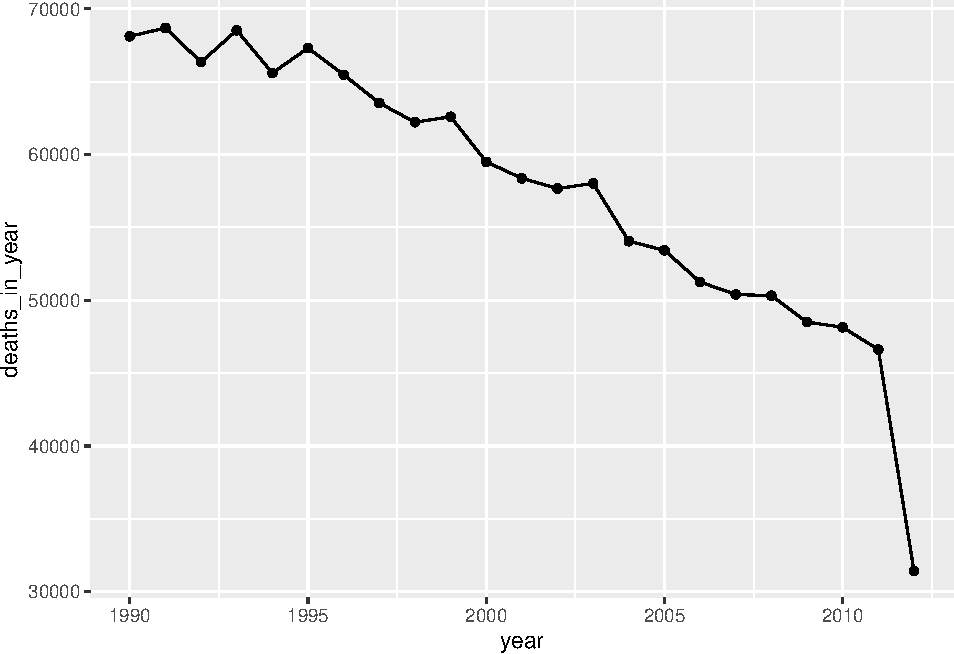
\includegraphics{adv_epi_analysis_files/figure-latex/unnamed-chunk-7-1.pdf}

\begin{enumerate}
\def\labelenumi{\arabic{enumi}.}
\setcounter{enumi}{1}
\tightlist
\item
  \textbf{Are there any missing dates within this time period? Are there any recorded
  dates where health outcome measurements are missing?
  Any where exposure measurements are missing?}
\end{enumerate}

There are a few things you should check to answer this question. First
(and easiest), you can check to see if there are any \texttt{NA} values within
any of the observations in the dataset. This helps answer the second and third
parts of the question. The \texttt{summary} function will provide
a summary of the values in each column of the dataset, including the count
of missing values (\texttt{NA}s) if there are any:

\begin{Shaded}
\begin{Highlighting}[]
\FunctionTok{summary}\NormalTok{(obs)}
\end{Highlighting}
\end{Shaded}

\begin{verbatim}
##       date                 year          month             day       
##  Min.   :1990-01-01   Min.   :1990   Min.   : 1.000   Min.   : 1.00  
##  1st Qu.:1995-09-01   1st Qu.:1995   1st Qu.: 3.000   1st Qu.: 8.00  
##  Median :2001-05-02   Median :2001   Median : 6.000   Median :16.00  
##  Mean   :2001-05-02   Mean   :2001   Mean   : 6.464   Mean   :15.73  
##  3rd Qu.:2006-12-31   3rd Qu.:2006   3rd Qu.: 9.000   3rd Qu.:23.00  
##  Max.   :2012-08-31   Max.   :2012   Max.   :12.000   Max.   :31.00  
##       doy            dow                 all           all_0_64   
##  Min.   :  1.0   Length:8279        Min.   : 81.0   Min.   : 9.0  
##  1st Qu.: 90.5   Class :character   1st Qu.:138.0   1st Qu.:27.0  
##  Median :180.0   Mode  :character   Median :157.0   Median :32.0  
##  Mean   :181.3                      Mean   :160.2   Mean   :32.4  
##  3rd Qu.:272.0                      3rd Qu.:178.0   3rd Qu.:37.0  
##  Max.   :366.0                      Max.   :363.0   Max.   :64.0  
##    all_65_74       all_75_84        all_85plus         tmean       
##  Min.   : 6.00   Min.   : 17.00   Min.   : 17.00   Min.   :-5.503  
##  1st Qu.:23.00   1st Qu.: 41.00   1st Qu.: 39.00   1st Qu.: 7.470  
##  Median :29.00   Median : 49.00   Median : 45.00   Median :11.465  
##  Mean   :30.45   Mean   : 50.65   Mean   : 46.68   Mean   :11.614  
##  3rd Qu.:37.00   3rd Qu.: 58.00   3rd Qu.: 53.00   3rd Qu.:15.931  
##  Max.   :70.00   Max.   :138.00   Max.   :128.00   Max.   :29.143  
##       tmin             tmax       
##  Min.   :-8.940   Min.   :-3.785  
##  1st Qu.: 3.674   1st Qu.:10.300  
##  Median : 7.638   Median :14.782  
##  Mean   : 7.468   Mean   :15.058  
##  3rd Qu.:11.438   3rd Qu.:19.830  
##  Max.   :20.438   Max.   :37.087
\end{verbatim}

Based on this analysis, all observations are complete for all dates included
in the dataset. There are no listings for \texttt{NA}s for any of the columns, and
this indicates no missing values in the dates for which there's a row in the data.

However, this does not guarantee that every date between the start date and
end date of the study period are included in the recorded data. Sometimes,
some dates might not get recorded at all in the dataset, and the \texttt{summary}
function won't help you determine when this is the case. One common example in
environmental epidemiology is with ozone pollution data. These are sometimes
only measured in the warm season, and so may be shared in a dataset with all
dates outside of the warm season excluded.

There are a few alternative explorations you can do to check this. Perhaps the
easiest is to check
the number of days between the start and end date of the study period, and
then see if the number of observations in the dataset is the same:

\begin{Shaded}
\begin{Highlighting}[]
\CommentTok{\# Calculate number of days in study period}
\NormalTok{obs }\SpecialCharTok{\%\textgreater{}\%}            \CommentTok{\# Using piping (\%\textgreater{}\%) throughout to keep code clear}
  \FunctionTok{pull}\NormalTok{(date) }\SpecialCharTok{\%\textgreater{}\%}   \CommentTok{\# Extract the \textasciigrave{}date\textasciigrave{} column as a vector}
  \FunctionTok{range}\NormalTok{() }\SpecialCharTok{\%\textgreater{}\%}      \CommentTok{\# Take the range of dates (earliest and latest)}
  \FunctionTok{diff}\NormalTok{()           }\CommentTok{\# Calculate time difference from start to finish of study }
\end{Highlighting}
\end{Shaded}

\begin{verbatim}
## Time difference of 8278 days
\end{verbatim}

\begin{Shaded}
\begin{Highlighting}[]
\CommentTok{\# Get number of observations in dataset{-}{-}{-}should be 1 more than time difference}
\NormalTok{obs }\SpecialCharTok{\%\textgreater{}\%} 
  \FunctionTok{nrow}\NormalTok{()}
\end{Highlighting}
\end{Shaded}

\begin{verbatim}
## [1] 8279
\end{verbatim}

This indicates that there is an observation for every date over the study period,
since the number of observations should be one more than the time difference.
In the next question, we'll be plotting observations by time, and typically this
will also help you see if there are large chunks of missing dates in the data.

\begin{enumerate}
\def\labelenumi{\arabic{enumi}.}
\setcounter{enumi}{2}
\tightlist
\item
  \textbf{Are there seasonal trends in the exposure? In the outcome?}
\end{enumerate}

You can use a simple plot to visualize patterns over time in both the exposure
and the outcome. For example, the following code plots a dot for each daily
temperature observation over the study period. The points are set to a smaller
size (\texttt{size\ =\ 0.5}) and plotted with some transparency (\texttt{alpha\ =\ 0.5}) since
there are so many observations.

\begin{Shaded}
\begin{Highlighting}[]
\FunctionTok{ggplot}\NormalTok{(obs, }\FunctionTok{aes}\NormalTok{(}\AttributeTok{x =}\NormalTok{ date, }\AttributeTok{y =}\NormalTok{ tmean)) }\SpecialCharTok{+} 
  \FunctionTok{geom\_point}\NormalTok{(}\AttributeTok{alpha =} \FloatTok{0.5}\NormalTok{, }\AttributeTok{size =} \FloatTok{0.5}\NormalTok{)}
\end{Highlighting}
\end{Shaded}

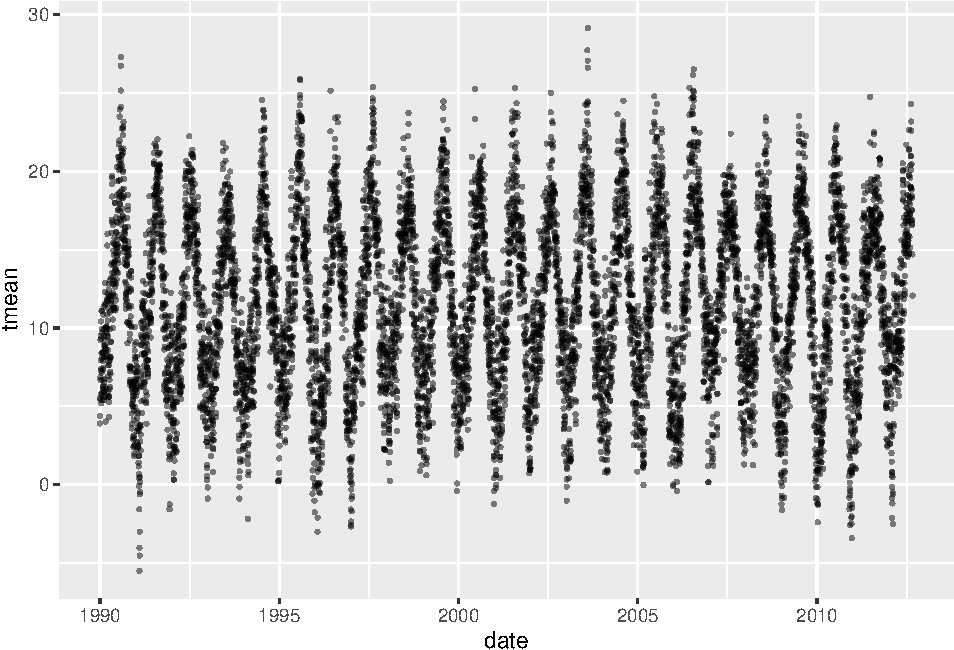
\includegraphics{adv_epi_analysis_files/figure-latex/unnamed-chunk-10-1.pdf}

There is (unsurprisingly) clear evidence here of a strong seasonal trend in mean temperature,
with values typically lowest in the winter and highest in the summer.

You can plot the outcome variable in the same way:

\begin{Shaded}
\begin{Highlighting}[]
\FunctionTok{ggplot}\NormalTok{(obs, }\FunctionTok{aes}\NormalTok{(}\AttributeTok{x =}\NormalTok{ date, }\AttributeTok{y =}\NormalTok{ all)) }\SpecialCharTok{+} 
  \FunctionTok{geom\_point}\NormalTok{(}\AttributeTok{alpha =} \FloatTok{0.5}\NormalTok{, }\AttributeTok{size =} \FloatTok{0.5}\NormalTok{)}
\end{Highlighting}
\end{Shaded}

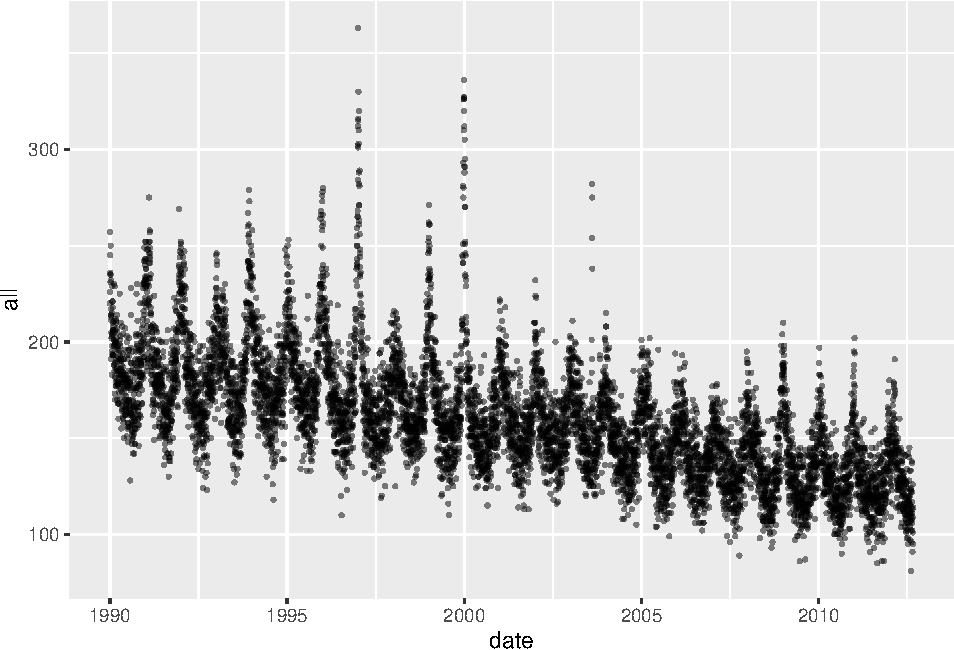
\includegraphics{adv_epi_analysis_files/figure-latex/unnamed-chunk-11-1.pdf}

Again, there are seasonal trends, although in this case they are inversed.
Mortality tends to be highest in the winter and lowest in the summer. Further, the
seasonal pattern is not equally strong in all years---some years it has a much
higher winter peak, probably in conjunction with severe influenza seasons.

Another way to look for seasonal trends is with a heatmap-style visualization,
with day of year along the x-axis and year along the y-axis. This allows you
to see patterns that repeat around the same time of the year each year (and
also unusual deviations from normal seasonal patterns).

For example, here's a plot showing temperature in each year, where the
observations are aligned on the x-axis by time in year. We're using the \texttt{doy}---which stands for ``day of year'' (i.e., Jan 1 = 1; Jan 2 = 2; \ldots{} Dec 31 = 365 as long
as it's not a leap year) as the measure of time in the year. We've reversed
the y-axis so that the earliest years in the study period start at the top
of the visual, then later study years come later---this is a personal style,
and it would be no problem to leave the y-axis as-is. We've used the
\texttt{viridis} color scale for the fill, since that has a number of features
that make it preferable to the default R color scale, including that it
is perceptible for most types of color blindness and be printed out in grayscale
and still be correctly interpreted.

\begin{Shaded}
\begin{Highlighting}[]
\FunctionTok{library}\NormalTok{(viridis)}
\FunctionTok{ggplot}\NormalTok{(obs, }\FunctionTok{aes}\NormalTok{(}\AttributeTok{x =}\NormalTok{ doy, }\AttributeTok{y =}\NormalTok{ year, }\AttributeTok{fill =}\NormalTok{ tmean)) }\SpecialCharTok{+} 
  \FunctionTok{geom\_tile}\NormalTok{() }\SpecialCharTok{+}
  \FunctionTok{scale\_y\_reverse}\NormalTok{() }\SpecialCharTok{+} 
  \FunctionTok{scale\_fill\_viridis}\NormalTok{()}
\end{Highlighting}
\end{Shaded}

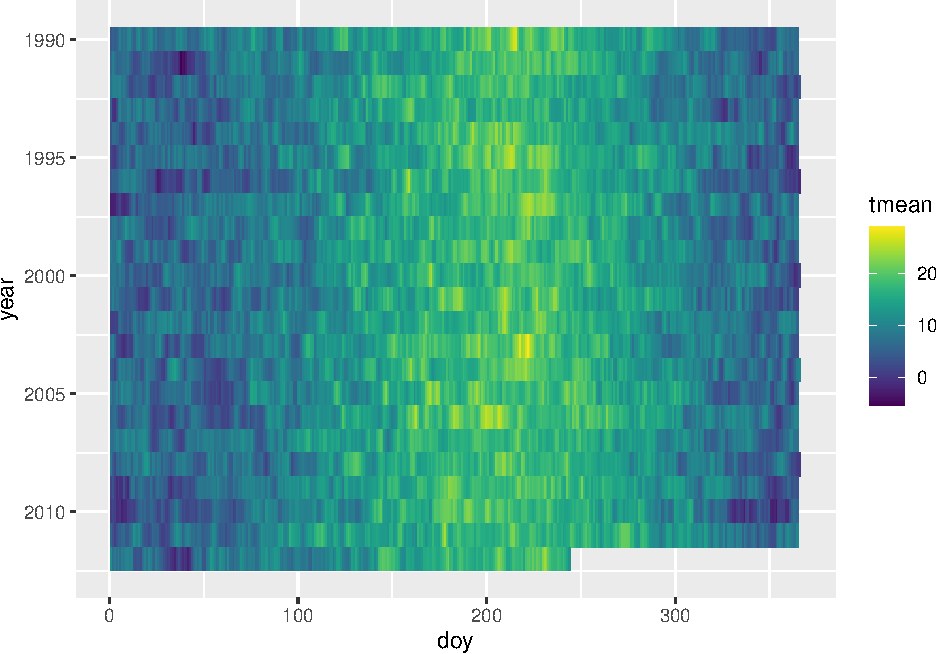
\includegraphics{adv_epi_analysis_files/figure-latex/unnamed-chunk-12-1.pdf}

From this visualization, you can see that temperatures tend to be higher in the
summer months and lower in the winter months. ``Spells'' of extreme heat or cold
are visible---where extreme temperatures tend to persist over a period, rather
than randomly fluctuating within a season. You can also see unusual events, like
the extreme heat wave in the summer of 2003, indicated with the brightest
yellow in the plot.

We created the same style of plot for the health outcome. In this case, we
focused on mortality among the oldest age group, as temperature sensitivity
tends to increase with age, so this might be where the strongest patterns are
evident.

\begin{Shaded}
\begin{Highlighting}[]
\FunctionTok{ggplot}\NormalTok{(obs, }\FunctionTok{aes}\NormalTok{(}\AttributeTok{x =}\NormalTok{ doy, }\AttributeTok{y =}\NormalTok{ year, }\AttributeTok{fill =}\NormalTok{ all\_85plus)) }\SpecialCharTok{+} 
  \FunctionTok{geom\_tile}\NormalTok{() }\SpecialCharTok{+}
  \FunctionTok{scale\_y\_reverse}\NormalTok{() }\SpecialCharTok{+} 
  \FunctionTok{scale\_fill\_viridis}\NormalTok{()}
\end{Highlighting}
\end{Shaded}

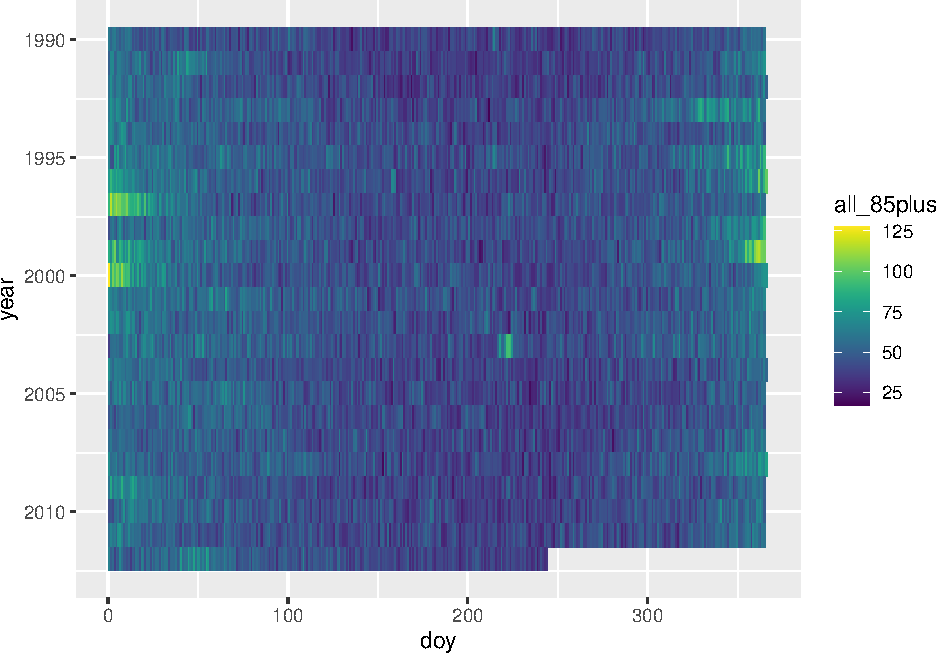
\includegraphics{adv_epi_analysis_files/figure-latex/unnamed-chunk-13-1.pdf}

For mortality, there tends to be an increase in the winter compared to the summer.
Some winters have stretches with particularly high mortality---these are likely
a result of seasons with strong influenza outbreaks. You can also see on this
plot the impact of the 2003 heat wave on mortality among this oldest age group---an
unusual spot of light green in the summer.

\begin{enumerate}
\def\labelenumi{\arabic{enumi}.}
\setcounter{enumi}{3}
\tightlist
\item
  \textbf{Are there long-term trends in the exposure? In the outcome?}
\end{enumerate}

Some of the plots we created in the last section help in exploring this
question. For example, the following plot shows a clear pattern of decreasing
daily mortality counts, on average, over the course of the study period:

\begin{Shaded}
\begin{Highlighting}[]
\FunctionTok{ggplot}\NormalTok{(obs, }\FunctionTok{aes}\NormalTok{(}\AttributeTok{x =}\NormalTok{ date, }\AttributeTok{y =}\NormalTok{ all)) }\SpecialCharTok{+} 
  \FunctionTok{geom\_point}\NormalTok{(}\AttributeTok{alpha =} \FloatTok{0.5}\NormalTok{, }\AttributeTok{size =} \FloatTok{0.5}\NormalTok{)}
\end{Highlighting}
\end{Shaded}

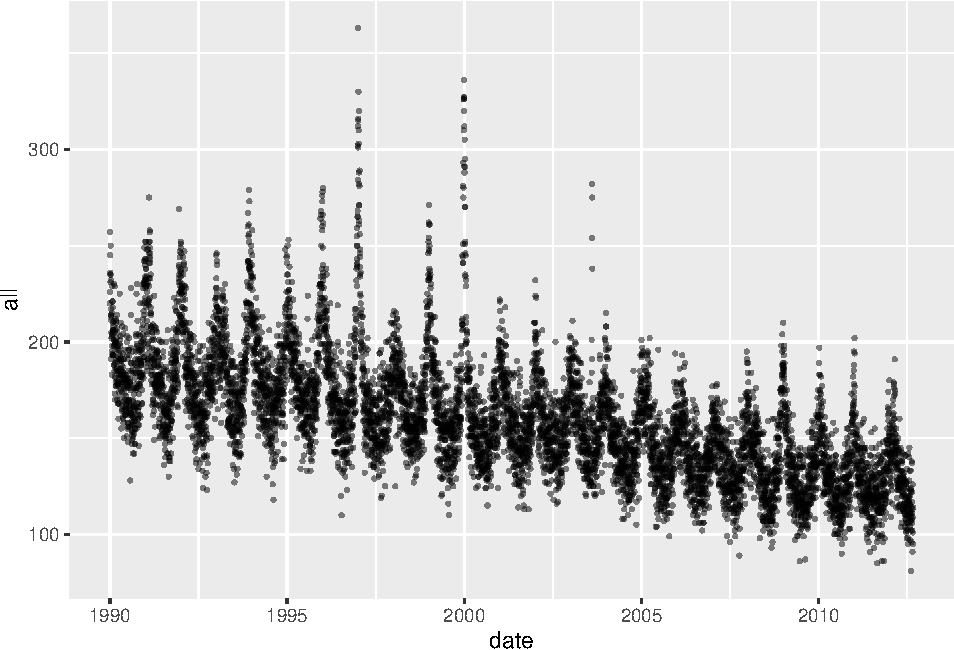
\includegraphics{adv_epi_analysis_files/figure-latex/unnamed-chunk-14-1.pdf}

It can be helpful to add a smooth line to help detect these longer-term
patterns, which you can do with \texttt{geom\_smooth}:

\begin{Shaded}
\begin{Highlighting}[]
\FunctionTok{ggplot}\NormalTok{(obs, }\FunctionTok{aes}\NormalTok{(}\AttributeTok{x =}\NormalTok{ date, }\AttributeTok{y =}\NormalTok{ all)) }\SpecialCharTok{+} 
  \FunctionTok{geom\_point}\NormalTok{(}\AttributeTok{alpha =} \FloatTok{0.5}\NormalTok{, }\AttributeTok{size =} \FloatTok{0.5}\NormalTok{) }\SpecialCharTok{+} 
  \FunctionTok{geom\_smooth}\NormalTok{()}
\end{Highlighting}
\end{Shaded}

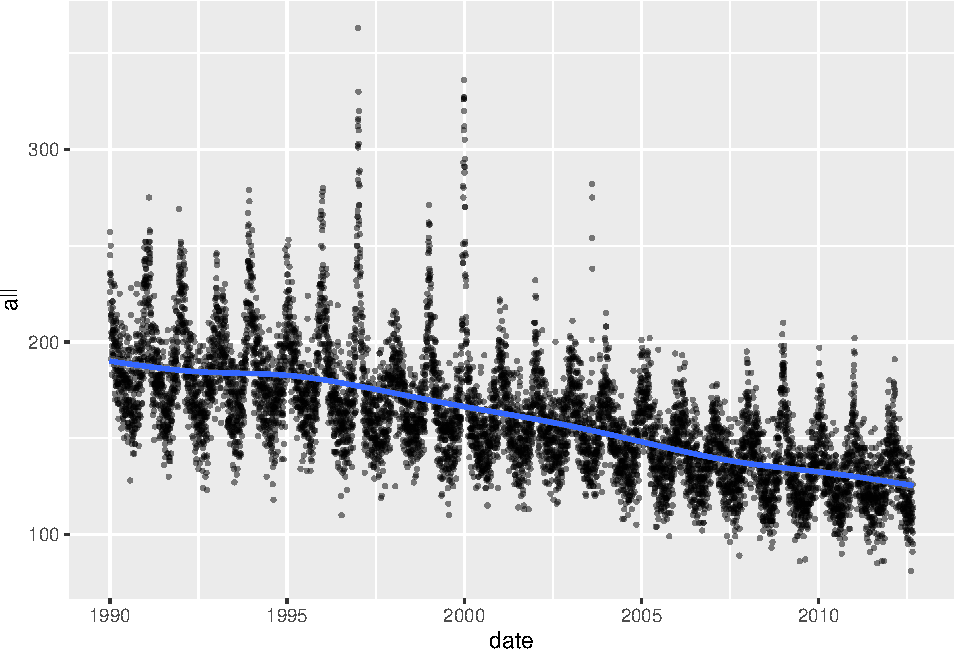
\includegraphics{adv_epi_analysis_files/figure-latex/unnamed-chunk-15-1.pdf}

You could also take the median mortality count across each year in the
study period, although you should take out any years without a full year's
worth of data before you do this, since there are seasonal trends in the
outcome:

\begin{Shaded}
\begin{Highlighting}[]
\NormalTok{obs }\SpecialCharTok{\%\textgreater{}\%} 
  \FunctionTok{group\_by}\NormalTok{(year) }\SpecialCharTok{\%\textgreater{}\%} 
  \FunctionTok{filter}\NormalTok{(year }\SpecialCharTok{!=} \DecValTok{2012}\NormalTok{) }\SpecialCharTok{\%\textgreater{}\%} \CommentTok{\# Take out the last year}
  \FunctionTok{summarize}\NormalTok{(}\AttributeTok{median\_mort =} \FunctionTok{median}\NormalTok{(all)) }\SpecialCharTok{\%\textgreater{}\%} 
  \FunctionTok{ggplot}\NormalTok{(}\FunctionTok{aes}\NormalTok{(}\AttributeTok{x =}\NormalTok{ year, }\AttributeTok{y =}\NormalTok{ median\_mort)) }\SpecialCharTok{+}
  \FunctionTok{geom\_line}\NormalTok{()}
\end{Highlighting}
\end{Shaded}

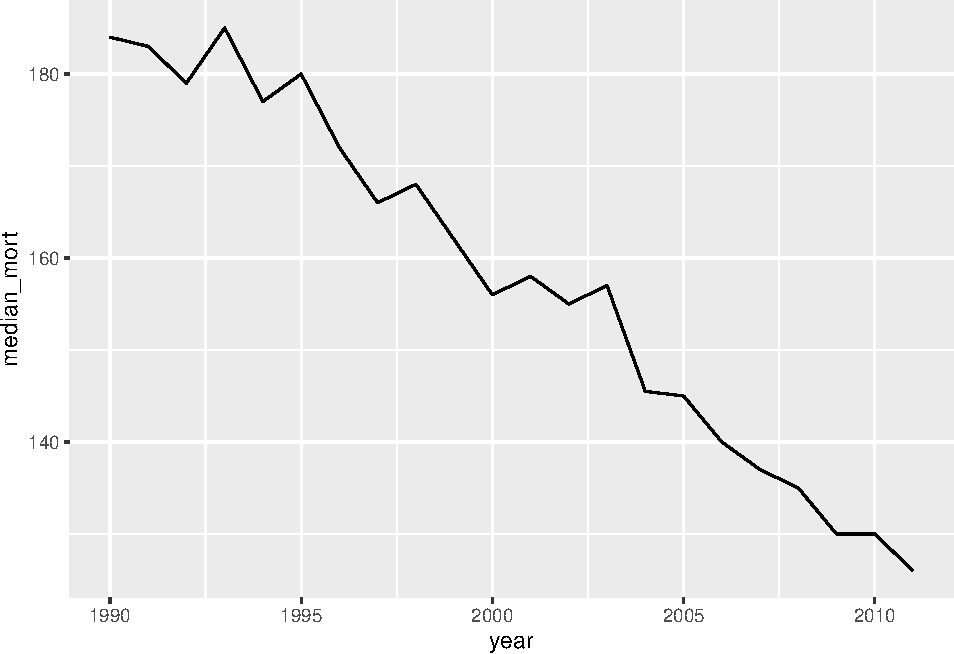
\includegraphics{adv_epi_analysis_files/figure-latex/unnamed-chunk-16-1.pdf}

Again, we see a clear pattern of decreasing mortality rates in this city over time.
This means we need to think carefully about long-term time patterns as a potential
confounder. It will be particularly important to think about this if the exposure
also has a strong pattern over time. For example, air pollution regulations have
meant that, in many cities, there may be long-term decreases in pollution
concentrations over a study period.

\begin{enumerate}
\def\labelenumi{\arabic{enumi}.}
\setcounter{enumi}{4}
\tightlist
\item
  \textbf{Is the outcome associated with day of week? Is the exposure associated
  with day of week?}
\end{enumerate}

The data already has day of week as a column in the data (\texttt{dow}). However,
this is in a character data type, so it doesn't have the order of weekdays
encoded (e.g., Monday comes before Tuesday). This makes it hard to look for
patterns related to things like weekend / weekday.

\begin{Shaded}
\begin{Highlighting}[]
\FunctionTok{class}\NormalTok{(obs}\SpecialCharTok{$}\NormalTok{dow)}
\end{Highlighting}
\end{Shaded}

\begin{verbatim}
## [1] "character"
\end{verbatim}

We could convert this to a factor and encode the weekday order when we do
it, but it's even easier to just recreate the column from the \texttt{date} column.
We used the \texttt{wday} function from the \texttt{lubridate} package to do this---it extracts
weekday as a factor, with the order of weekdays encoded (using a special
``ordered'' factor type):

\begin{Shaded}
\begin{Highlighting}[]
\FunctionTok{library}\NormalTok{(lubridate)}
\NormalTok{obs }\OtherTok{\textless{}{-}}\NormalTok{ obs }\SpecialCharTok{\%\textgreater{}\%} 
  \FunctionTok{mutate}\NormalTok{(}\AttributeTok{dow =} \FunctionTok{wday}\NormalTok{(date, }\AttributeTok{label =} \ConstantTok{TRUE}\NormalTok{))}

\FunctionTok{class}\NormalTok{(obs}\SpecialCharTok{$}\NormalTok{dow)}
\end{Highlighting}
\end{Shaded}

\begin{verbatim}
## [1] "ordered" "factor"
\end{verbatim}

\begin{Shaded}
\begin{Highlighting}[]
\FunctionTok{levels}\NormalTok{(obs}\SpecialCharTok{$}\NormalTok{dow)}
\end{Highlighting}
\end{Shaded}

\begin{verbatim}
## [1] "Sun" "Mon" "Tue" "Wed" "Thu" "Fri" "Sat"
\end{verbatim}

We looked at the mean, median, and 25th and 75th quantiles of the mortality
counts by day of week:

\begin{Shaded}
\begin{Highlighting}[]
\NormalTok{obs }\SpecialCharTok{\%\textgreater{}\%} 
  \FunctionTok{group\_by}\NormalTok{(dow) }\SpecialCharTok{\%\textgreater{}\%} 
  \FunctionTok{summarize}\NormalTok{(}\FunctionTok{mean}\NormalTok{(all), }
            \FunctionTok{median}\NormalTok{(all), }
            \FunctionTok{quantile}\NormalTok{(all, }\FloatTok{0.25}\NormalTok{), }
            \FunctionTok{quantile}\NormalTok{(all, }\FloatTok{0.75}\NormalTok{))}
\end{Highlighting}
\end{Shaded}

\begin{verbatim}
## # A tibble: 7 x 5
##   dow   `mean(all)` `median(all)` `quantile(all, 0.25)` `quantile(all, 0.75)`
##   <ord>       <dbl>         <dbl>                 <dbl>                 <dbl>
## 1 Sun          156.           154                  136                    173
## 2 Mon          161.           159                  138                    179
## 3 Tue          161.           158                  139                    179
## 4 Wed          160.           157                  138.                   179
## 5 Thu          161.           158                  139                    179
## 6 Fri          162.           159                  141                    179
## 7 Sat          159.           156                  137                    178
\end{verbatim}

Mortality tends to be a bit higher on weekdays than weekends, but it's not
a dramatic difference.

We did the same check for temperature:

\begin{Shaded}
\begin{Highlighting}[]
\NormalTok{obs }\SpecialCharTok{\%\textgreater{}\%} 
  \FunctionTok{group\_by}\NormalTok{(dow) }\SpecialCharTok{\%\textgreater{}\%} 
  \FunctionTok{summarize}\NormalTok{(}\FunctionTok{mean}\NormalTok{(tmean), }
            \FunctionTok{median}\NormalTok{(tmean), }
            \FunctionTok{quantile}\NormalTok{(tmean, }\FloatTok{0.25}\NormalTok{), }
            \FunctionTok{quantile}\NormalTok{(tmean, }\FloatTok{0.75}\NormalTok{))}
\end{Highlighting}
\end{Shaded}

\begin{verbatim}
## # A tibble: 7 x 5
##   dow   `mean(tmean)` `median(tmean)` `quantile(tmean, 0.25)`
##   <ord>         <dbl>           <dbl>                   <dbl>
## 1 Sun            11.6            11.3                    7.48
## 2 Mon            11.6            11.4                    7.33
## 3 Tue            11.5            11.4                    7.48
## 4 Wed            11.7            11.7                    7.64
## 5 Thu            11.6            11.5                    7.57
## 6 Fri            11.6            11.6                    7.41
## 7 Sat            11.6            11.5                    7.53
## # i 1 more variable: `quantile(tmean, 0.75)` <dbl>
\end{verbatim}

In this case, there does not seem to be much of a pattern by weekday.

You can also visualize the association using boxplots:

\begin{Shaded}
\begin{Highlighting}[]
\FunctionTok{ggplot}\NormalTok{(obs, }\FunctionTok{aes}\NormalTok{(}\AttributeTok{x =} \FunctionTok{wday}\NormalTok{(date, }\AttributeTok{label =} \ConstantTok{TRUE}\NormalTok{), }\AttributeTok{y =}\NormalTok{ all)) }\SpecialCharTok{+} 
  \FunctionTok{geom\_boxplot}\NormalTok{()}
\end{Highlighting}
\end{Shaded}

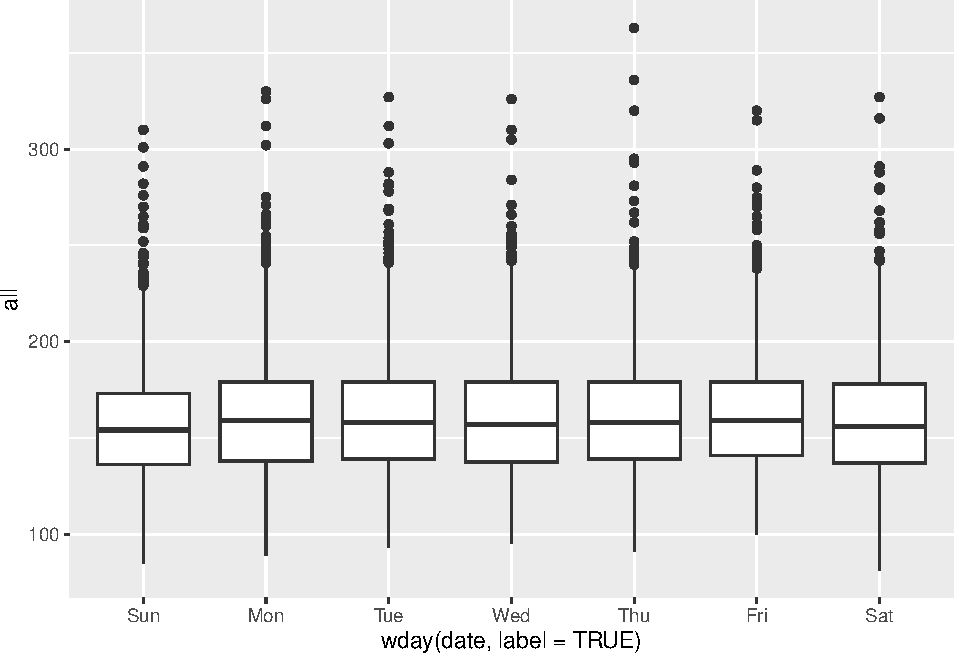
\includegraphics{adv_epi_analysis_files/figure-latex/unnamed-chunk-21-1.pdf}

You can also try violin plots---these show the full distribution better than
boxplots, which only show quantiles.

\begin{Shaded}
\begin{Highlighting}[]
\FunctionTok{ggplot}\NormalTok{(obs, }\FunctionTok{aes}\NormalTok{(}\AttributeTok{x =}\NormalTok{ dow, }\AttributeTok{y =}\NormalTok{ all)) }\SpecialCharTok{+} 
  \FunctionTok{geom\_violin}\NormalTok{(}\AttributeTok{draw\_quantiles =} \FunctionTok{c}\NormalTok{(}\FloatTok{0.25}\NormalTok{, }\FloatTok{0.5}\NormalTok{, }\FloatTok{0.75}\NormalTok{))}
\end{Highlighting}
\end{Shaded}

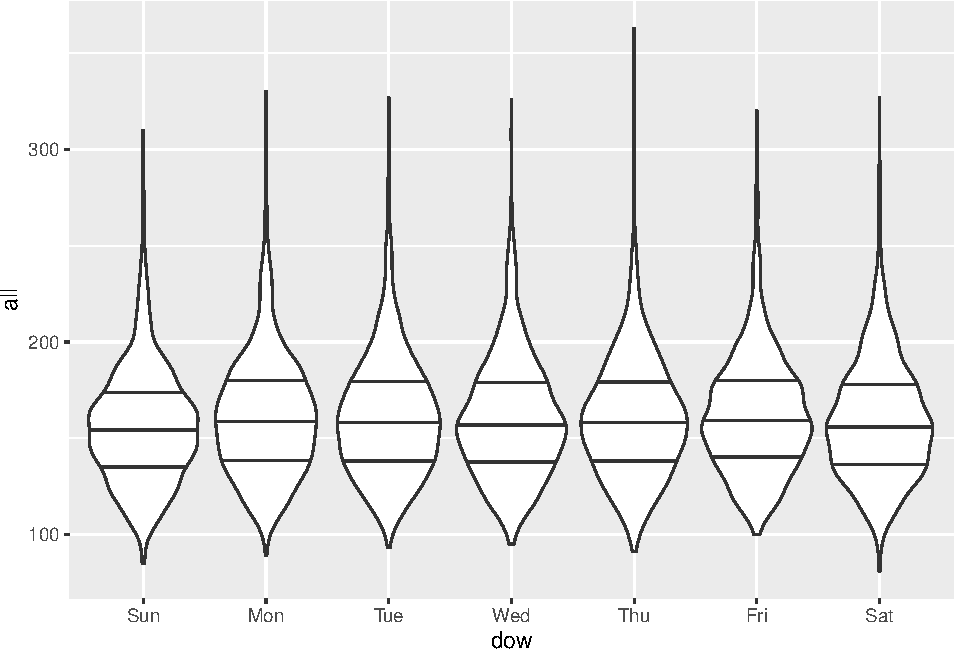
\includegraphics{adv_epi_analysis_files/figure-latex/unnamed-chunk-22-1.pdf}

All these reinforce that there are some small differences in weekend versus weekday
patterns for mortality. There isn't much pattern by weekday with temperature, so
in this case weekday is unlikely to be a confounder (the same is not true with
air pollution, which often varies based on commuting patterns and so can have
stronger weekend/weekday differences). However, since it does help some in explaining
variation in the health outcome, it might be worth including in our models anyway,
to help reduce random noise.

Exploratory data analysis is an excellent tool for exploring your data before
you begin fitting a statistical model, and you should get in the habit of using
it regularly in your research. \citet{dominici2008statistical5} provides another walk-through of exploring this type of data, including some more advanced tools
for exploring autocorrelation and time patterns.

\section{Statistical modeling for a time series study}\label{statistical-modeling-for-a-time-series-study}

Now that we've explored the data typical of a time series study in climate
epidemiology, we'll look at how we can fit a statistical model to those
data to gain insight into the relationship between the exposure and
acute health effects. Very broadly, we'll be using a statistical model to answer
the question: How does the relative risk of a health outcome change as
the level of the exposure changes, after controlling for potential confounders?

In the rest of this chapter and the next chapter, we'll
move step-by-step to build up to the statistical models that are now typically
used in these studies.
Along the way, we'll discuss key components and choices in this modeling process.
The statistical modeling is based heavily on regression modeling, and specifically
generalized linear regression. To help you get the most of this section, you
may find it helpful to review regression modeling and generalized linear models.
Some resources for that include \citet{dunn2018generalized1} and \citet{james2013introduction3} .

One of the readings for this week, \citet{vicedo2019hands}, includes a section
on fitting exposure-response functions to describe the association between
daily mean temperature and mortality risk. This article includes example
code in its supplemental material, with code for fitting the model to
these time series data in the file named ``01EstimationERassociation.r''.
Please download that file and take a look at the code.

The model in the code may at first seem complex, but it is made up of a number of
fairly straightforward pieces (although some may initially seem complex):

\begin{itemize}
\tightlist
\item
  The model framework is a \emph{generalized linear model (GLM)}
\item
  This GLM is fit assuming an \emph{error distribution} and a \emph{link function}
  appropriate for count data
\item
  The GLM is fit assuming an \emph{error distribution} that is also appropriate for
  data that may be \emph{overdispersed}
\item
  The model includes control for day of the week by including a \emph{categorical
  variable}
\item
  The model includes control for long-term and seasonal trends by including
  a \emph{spline} (in this case, a \emph{natural cubic spline}) for the day in the study
\item
  The model fits a flexible, non-linear association between temperature
  and mortality risk, also using a spline
\item
  The model fits a flexible non-linear association between temperature on
  a series of preceeding days and current day and mortality risk on the
  current day using a \emph{distributed lag approach}
\item
  The model jointly describes both of the two previous non-linear associations
  by fitting these two elements through one construct in the GLM, a
  \emph{cross-basis term}
\end{itemize}

In this section and the next chapter, we will work through the elements,
building up the code to get to the full model that is fit in \citet{vicedo2019hands}.

\emph{Fitting a GLM to time series data}

The generalized linear model (GLM) framework unites a number of types of
regression models you may have previously worked with. One basic regression
model that can be fit within this framework is a linear regression model.
However, the framework also allows you to also fit, among others, logistic
regression models (useful when the outcome variable can only take one of two
values, e.g., success / failure or alive / dead) and Poisson regression models
(useful when the outcome variable is a count or rate). This generalized
framework brings some unity to these different types of regression models. From
a practical standpoint, it has allowed software developers to easily provide a
common interface to fit these types of models. In R, the common function call to
fit GLMs is \texttt{glm}.

Within the GLM framework, the elements that separate different regression models
include the link function and the error distribution. The error distribution
encodes the assumption you are enforcing about how the errors after fitting the
model are distributed. If the outcome data are normally distributed (a.k.a.,
follow a Gaussian distribution), after accounting for variance explained in the
outcome by any of the model covariates, then a linear regression model may be
appropriate. For count data---like numbers of deaths a day---this is unlikely,
unless the average daily mortality count is very high (count data tend to
come closer to a normal distribution the further their average gets from
0). For binary data---like whether each person in a study population died on
a given day or not---normally distributed errors are also unlikely. Instead,
in these two cases, it is typically more appropriate to fit GLMs with
Poisson and binomial ``families'', respectively, where the family designation
includes an appropriate specification for the variance when fitting the model
based on these outcome types.

The other element that distinguishes different types of regression within
the GLM framework is the link function. The link function applies a transformation
on the combination of independent variables in the regression equation
when fitting the model. With normally distributed data, an \emph{identity link}
is often appropriate---with this link, the combination of independent variables
remain unchanged (i.e., keep their initial ``identity''). With count data, a
\emph{log link} is often more appropriate, while with binomial data, a \emph{logit link}
is often used.

Finally, data will often not perfectly adhere to assumptions. For example, the
Poisson family of GLMs assumes that variance follows a Poisson distribution
(The probability mass function for Poisson distribution \(X \sim {\sf Poisson}(\mu)\) is denoted by \(f(k;\mu)=Pr[X=k]= \displaystyle \frac{\mu^{k}e^{-\mu}}{k!}\), where
\(k\) is the number of occurences, and \(\mu\) is equal to the expected number of
cases). With this distribution, the variance is equal to the mean (\(\mu=E(X)=Var(X)\)). With real-life data, this assumption is often not valid, and in many cases the variance in real life count data is larger than the mean. This can be accounted for when fitting a GLM by setting an error distribution that does not require the variance to equal the mean---instead, both a mean value and something like a
variance are estimated from the data, assuming an overdispersion parameter \(\phi\)
so that \(Var(X)=\phi E(X)\). In environmental epidemiology, time series
are often fit to allow for this overdispersion. This is because if the data are overdispersed but the model does not account for this, the standard errors on the
estimates of the model parameters may be artificially small. If the data are not overdispersed (\(\phi=1\)), the model will identify this when being fit to the data,
so it is typically better to prefer to allow for overdispersion in the model
(if the size of the data were small, you may want to be parsimonious and avoid
unneeded complexity in the model, but this is typically not the case with time
series data).

In the next section, you will work through the steps of developing a GLM to fit
the example dataset \texttt{obs}. For now, you will only fit a linear association
between mean daily temperature and mortality risk, eventually including control
for day of week. In later work, especially the next chapter, we will build up
other components of the model, including control for the potential confounders
of long-term and seasonal patterns, as well as advancing the model to fit
non-linear associations, distributed by time, through splines, a distributed lag
approach, and a cross-basis term.

\emph{Applied: Fitting a GLM to time series data}

In R, the function call used to fit GLMs is \texttt{glm}. Most of you have likely
covered GLMs, and ideally this function call, in previous courses. If you are
unfamiliar with its basic use, you will want to refresh yourself on this
topic---you can use some of the resources noted earlier in this section and in
the chapter's ``Supplemental Readings'' to do so.

\begin{enumerate}
\def\labelenumi{\arabic{enumi}.}
\tightlist
\item
  Fit a GLM to estimate the association between mean daily temperature (as the
  independent variable) and daily mortality count (as the dependent variable),
  first fitting a linear regression. (Since the mortality data are counts, we will
  want to shift to a different type of regression within the GLM framework, but
  this step allows you to develop a simple \texttt{glm} call, and to remember where to
  include the data and the independent and dependent variables within this
  function call.)
\item
  Change your function call to fit a regression model in the Poisson family.
\item
  Change your function call to allow for overdispersion in the outcome data
  (daily mortality count). How does the estimated coefficient for temperature
  change between the model fit for \#2 and this model? Check both the central
  estimate and its estimated standard error.
\item
  Change your function call to include control for day of week.
\end{enumerate}

\emph{Applied exercise: Example code}

\begin{enumerate}
\def\labelenumi{\arabic{enumi}.}
\tightlist
\item
  \textbf{Fit a GLM to estimate the association between mean daily temperature (as the
  independent variable) and daily mortality count (as the dependent variable),
  first fitting a linear regression.}
\end{enumerate}

This is the model you are fitting:

\(Y_{t}=\beta_{0}+\beta_{1}X1_{t}+\epsilon\)

where \(Y_{t}\) is the mortality count on day \(t\), \(X1_{t}\) is the mean temperature
for day \(t\) and \(\epsilon\) is the error term. Since this is a linear model we are
assuming a Gaussian error distribution \(\epsilon \sim {\sf N}(0, \sigma^{2})\),
where \(\sigma^{2}\) is the variance not explained by the covariates (here just
temperature).

To do this, you will use the \texttt{glm} call. If you would like to save model fit
results to use later, you assign the output a name as an R object
(\texttt{mod\_linear\_reg} in the example code). If your study data are in a dataframe,
you can specify these data in the \texttt{glm} call with the \texttt{data} parameter.
Once you do this, you can use column names directly in the model formula.
In the model formula, the dependent variable is specified first (\texttt{all}, the
column for daily mortality counts for all ages, in this example), followed
by a tilde (\texttt{\textasciitilde{}}), followed by all independent variables (only \texttt{tmean} in this
example). If multiple independent variables are included, they are joined using
\texttt{+}. We'll see an example when we start adding control for confounders later.

\begin{Shaded}
\begin{Highlighting}[]
\NormalTok{mod\_linear\_reg }\OtherTok{\textless{}{-}} \FunctionTok{glm}\NormalTok{(all }\SpecialCharTok{\textasciitilde{}}\NormalTok{ tmean, }\AttributeTok{data =}\NormalTok{ obs)}
\end{Highlighting}
\end{Shaded}

Once you have fit a model and assigned it to an R object, you can explore it
and use resulting values. First, the \texttt{print} method for a regression model
gives some summary information. This method is automatically called if you
enter the model object's name at the console:

\begin{Shaded}
\begin{Highlighting}[]
\NormalTok{mod\_linear\_reg}
\end{Highlighting}
\end{Shaded}

\begin{verbatim}
## 
## Call:  glm(formula = all ~ tmean, data = obs)
## 
## Coefficients:
## (Intercept)        tmean  
##     187.647       -2.366  
## 
## Degrees of Freedom: 8278 Total (i.e. Null);  8277 Residual
## Null Deviance:       8161000 
## Residual Deviance: 6766000   AIC: 79020
\end{verbatim}

More information is printed if you run the \texttt{summary} method on the model
object:

\begin{Shaded}
\begin{Highlighting}[]
\FunctionTok{summary}\NormalTok{(mod\_linear\_reg)}
\end{Highlighting}
\end{Shaded}

\begin{verbatim}
## 
## Call:
## glm(formula = all ~ tmean, data = obs)
## 
## Coefficients:
##              Estimate Std. Error t value Pr(>|t|)    
## (Intercept) 187.64658    0.73557  255.10   <2e-16 ***
## tmean        -2.36555    0.05726  -41.31   <2e-16 ***
## ---
## Signif. codes:  0 '***' 0.001 '**' 0.01 '*' 0.05 '.' 0.1 ' ' 1
## 
## (Dispersion parameter for gaussian family taken to be 817.4629)
## 
##     Null deviance: 8161196  on 8278  degrees of freedom
## Residual deviance: 6766140  on 8277  degrees of freedom
## AIC: 79019
## 
## Number of Fisher Scoring iterations: 2
\end{verbatim}

Make sure you are familiar with the information provided from the model object,
as well as how to interpret values like the coefficient estimates and their
standard errors and p-values. These basic elements should have been covered in
previous coursework (even if a different programming language was used to fit
the model), and so we will not be covering them in great depth here, but instead
focusing on some of the more advanced elements of how regression models are
commonly fit to data from time series and case-crossover study designs in
environmental epidemiology. For a refresher on the basics of fitting
statistical models in R, you may want to check out Chapters 22 through 24 of
\citet{wickham2016r}, a book that is available online, as well as \citet{dunn2018generalized1} and
\citet{james2013introduction3} .

Finally, there are some newer tools for extracting information from model fit
objects. The \texttt{broom} package extracts different elements from these objects
and returns them in a ``tidy'' data format, which makes it much easier to use
the output further in analysis with functions from the ``tidyverse'' suite of
R packages. These tools are very popular and powerful, and so the \texttt{broom} tools
can be very useful in working with output from regression modeling in R.

The \texttt{broom} package includes three main functions for extracting data from
regression model objects. First, the \texttt{glance} function returns overall data
about the model fit, including the AIC and BIC:

\begin{Shaded}
\begin{Highlighting}[]
\FunctionTok{library}\NormalTok{(broom)}
\FunctionTok{glance}\NormalTok{(mod\_linear\_reg)}
\end{Highlighting}
\end{Shaded}

\begin{verbatim}
## # A tibble: 1 x 8
##   null.deviance df.null  logLik    AIC    BIC deviance df.residual  nobs
##           <dbl>   <int>   <dbl>  <dbl>  <dbl>    <dbl>       <int> <int>
## 1      8161196.    8278 -39507. 79019. 79041. 6766140.        8277  8279
\end{verbatim}

The \texttt{tidy} function returns data at the level of the model coefficients,
including the estimate for each model parameter, its standard error, test
statistic, and p-value.

\begin{Shaded}
\begin{Highlighting}[]
\FunctionTok{tidy}\NormalTok{(mod\_linear\_reg)}
\end{Highlighting}
\end{Shaded}

\begin{verbatim}
## # A tibble: 2 x 5
##   term        estimate std.error statistic p.value
##   <chr>          <dbl>     <dbl>     <dbl>   <dbl>
## 1 (Intercept)   188.      0.736      255.        0
## 2 tmean          -2.37    0.0573     -41.3       0
\end{verbatim}

Finally, the \texttt{augment} function returns data at the level of the original
observations, including the fitted value for each observation, the residual
between the fitted and true value, and some measures of influence on the model
fit.

\begin{Shaded}
\begin{Highlighting}[]
\FunctionTok{augment}\NormalTok{(mod\_linear\_reg)}
\end{Highlighting}
\end{Shaded}

\begin{verbatim}
## # A tibble: 8,279 x 8
##      all tmean .fitted .resid     .hat .sigma  .cooksd .std.resid
##    <dbl> <dbl>   <dbl>  <dbl>    <dbl>  <dbl>    <dbl>      <dbl>
##  1   220  3.91    178.   41.6 0.000359   28.6 0.000380       1.46
##  2   257  5.55    175.   82.5 0.000268   28.6 0.00112        2.89
##  3   245  4.39    177.   67.7 0.000330   28.6 0.000928       2.37
##  4   226  5.43    175.   51.2 0.000274   28.6 0.000440       1.79
##  5   236  6.87    171.   64.6 0.000211   28.6 0.000539       2.26
##  6   235  9.23    166.   69.2 0.000144   28.6 0.000420       2.42
##  7   231  6.69    172.   59.2 0.000218   28.6 0.000467       2.07
##  8   235  7.96    169.   66.2 0.000174   28.6 0.000467       2.31
##  9   250  7.27    170.   79.5 0.000197   28.6 0.000761       2.78
## 10   214  9.51    165.   48.9 0.000139   28.6 0.000202       1.71
## # i 8,269 more rows
\end{verbatim}

One way you can use \texttt{augment} is to graph the fitted values for each observation
after fitting the model:

\begin{Shaded}
\begin{Highlighting}[]
\NormalTok{mod\_linear\_reg }\SpecialCharTok{\%\textgreater{}\%} 
  \FunctionTok{augment}\NormalTok{() }\SpecialCharTok{\%\textgreater{}\%} 
  \FunctionTok{ggplot}\NormalTok{(}\FunctionTok{aes}\NormalTok{(}\AttributeTok{x =}\NormalTok{ tmean)) }\SpecialCharTok{+} 
  \FunctionTok{geom\_point}\NormalTok{(}\FunctionTok{aes}\NormalTok{(}\AttributeTok{y =}\NormalTok{ all), }\AttributeTok{alpha =} \FloatTok{0.4}\NormalTok{, }\AttributeTok{size =} \FloatTok{0.5}\NormalTok{) }\SpecialCharTok{+} 
  \FunctionTok{geom\_line}\NormalTok{(}\FunctionTok{aes}\NormalTok{(}\AttributeTok{y =}\NormalTok{ .fitted), }\AttributeTok{color =} \StringTok{"red"}\NormalTok{) }\SpecialCharTok{+} 
  \FunctionTok{labs}\NormalTok{(}\AttributeTok{x =} \StringTok{"Mean daily temperature"}\NormalTok{, }\AttributeTok{y =} \StringTok{"Expected mortality count"}\NormalTok{)}
\end{Highlighting}
\end{Shaded}

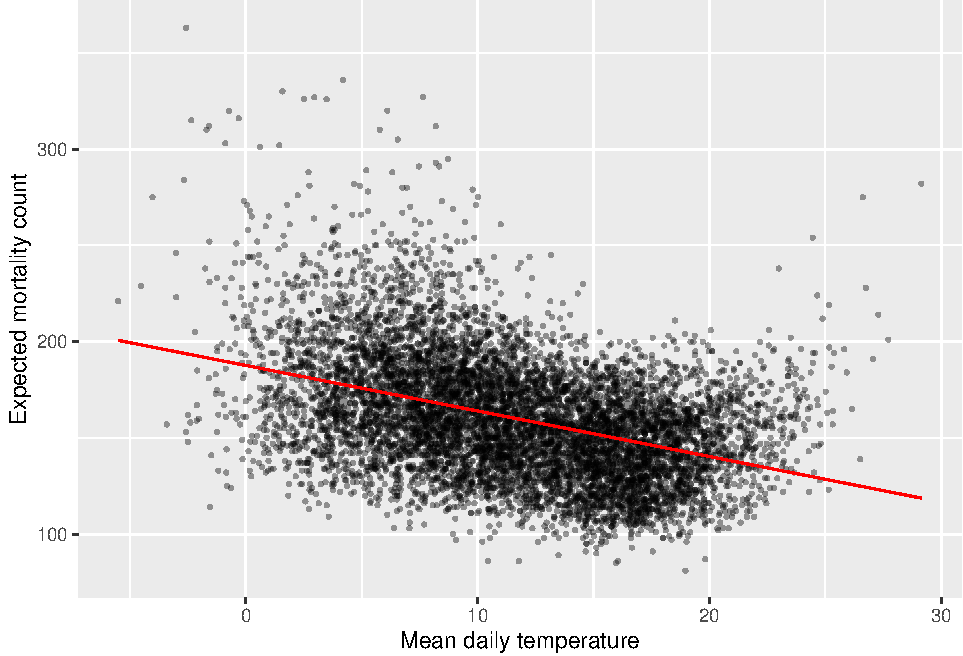
\includegraphics{adv_epi_analysis_files/figure-latex/unnamed-chunk-29-1.pdf}

For more on the \texttt{broom} package, including some excellent examples of how it
can be used to streamline complex regression analyses, see \citet{robinson2014broom}.
There is also a nice example of how it can be used in one of the chapters of
\citet{wickham2016r}, available online at \url{https://r4ds.had.co.nz/many-models.html}.

\begin{enumerate}
\def\labelenumi{\arabic{enumi}.}
\setcounter{enumi}{1}
\tightlist
\item
  \textbf{Change your function call to fit a regression model in the Poisson family.}
\end{enumerate}

A linear regression is often not appropriate when fitting a model where the
outcome variable provides counts, as with the example data, since such data
often don't follow a normal distribution. A Poisson regression
is typically preferred.

For a count distribution were \(Y \sim {\sf Poisson(\mu)}\) we typically fit a model
such as

\(g(Y)=\beta_{0}+\beta_{1}X1\), where \(g()\) represents the link function, in this
case a log function so that \(log(Y)=\beta_{0}+\beta_{1}X1\). We can also express
this as \(Y=exp(\beta_{0}+\beta_{1}X1)\).

In the \texttt{glm} call, you can specify this with the \texttt{family}
parameter, for which ``poisson'' is one choice.

\begin{Shaded}
\begin{Highlighting}[]
\NormalTok{mod\_pois\_reg }\OtherTok{\textless{}{-}} \FunctionTok{glm}\NormalTok{(all }\SpecialCharTok{\textasciitilde{}}\NormalTok{ tmean, }\AttributeTok{data =}\NormalTok{ obs, }\AttributeTok{family =} \StringTok{"poisson"}\NormalTok{)}
\end{Highlighting}
\end{Shaded}

One thing to keep in mind with this change is that the model now uses a
non-identity link between the combination of independent variable(s) and the
dependent variable. You will need to keep this in mind when you interpret
the estimates of the regression coefficients. While the coefficient estimate
for \texttt{tmean} from the linear regression could be interpreted as the expected
increase in mortality counts for a one-unit (i.e., one degree Celsius) increase
in temperature, now the estimated coefficient should be interpreted as the
expected increase in the natural log-transform of mortality count for a one-unit
increase in temperature.

\begin{Shaded}
\begin{Highlighting}[]
\FunctionTok{summary}\NormalTok{(mod\_pois\_reg)}
\end{Highlighting}
\end{Shaded}

\begin{verbatim}
## 
## Call:
## glm(formula = all ~ tmean, family = "poisson", data = obs)
## 
## Coefficients:
##               Estimate Std. Error z value Pr(>|z|)    
## (Intercept)  5.2445409  0.0019704 2661.67   <2e-16 ***
## tmean       -0.0147728  0.0001583  -93.29   <2e-16 ***
## ---
## Signif. codes:  0 '***' 0.001 '**' 0.01 '*' 0.05 '.' 0.1 ' ' 1
## 
## (Dispersion parameter for poisson family taken to be 1)
## 
##     Null deviance: 49297  on 8278  degrees of freedom
## Residual deviance: 40587  on 8277  degrees of freedom
## AIC: 97690
## 
## Number of Fisher Scoring iterations: 4
\end{verbatim}

You can see this even more clearly if you take a look at the association between
temperature for each observation and the expected mortality count fit by the
model. First, if you look at the fitted values without transforming, they
will still be in a state where mortality count is log-transformed. You can
see by looking at the range of the y-scale that these values are for the log
of expected mortality, rather than expected mortality (compare, for example, to
the similar plot shown from the first model, which was linear), and that the fitted
association for that \emph{transformation}, not for untransformed mortality counts, is linear:

\begin{Shaded}
\begin{Highlighting}[]
\NormalTok{mod\_pois\_reg }\SpecialCharTok{\%\textgreater{}\%} 
  \FunctionTok{augment}\NormalTok{() }\SpecialCharTok{\%\textgreater{}\%} 
  \FunctionTok{ggplot}\NormalTok{(}\FunctionTok{aes}\NormalTok{(}\AttributeTok{x =}\NormalTok{ tmean)) }\SpecialCharTok{+} 
  \FunctionTok{geom\_point}\NormalTok{(}\FunctionTok{aes}\NormalTok{(}\AttributeTok{y =} \FunctionTok{log}\NormalTok{(all)), }\AttributeTok{alpha =} \FloatTok{0.4}\NormalTok{, }\AttributeTok{size =} \FloatTok{0.5}\NormalTok{) }\SpecialCharTok{+} 
  \FunctionTok{geom\_line}\NormalTok{(}\FunctionTok{aes}\NormalTok{(}\AttributeTok{y =}\NormalTok{ .fitted), }\AttributeTok{color =} \StringTok{"red"}\NormalTok{) }\SpecialCharTok{+} 
  \FunctionTok{labs}\NormalTok{(}\AttributeTok{x =} \StringTok{"Mean daily temperature"}\NormalTok{, }\AttributeTok{y =} \StringTok{"Log(Expected mortality count)"}\NormalTok{)}
\end{Highlighting}
\end{Shaded}

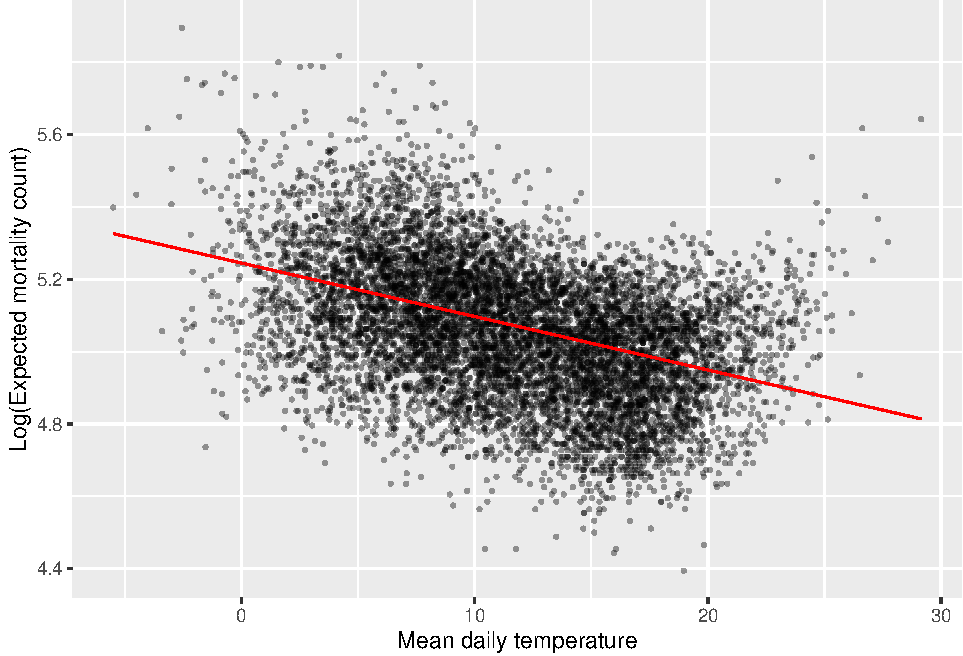
\includegraphics{adv_epi_analysis_files/figure-latex/unnamed-chunk-32-1.pdf}

You can use exponentiation to transform the fitted values back to just be the
expected mortality count based on the model fit. Once you make this
transformation, you can see how the link in the Poisson family specification
enforced a curved relationship between mean daily temperature and the
untransformed expected mortality count.

\begin{Shaded}
\begin{Highlighting}[]
\NormalTok{mod\_pois\_reg }\SpecialCharTok{\%\textgreater{}\%} 
  \FunctionTok{augment}\NormalTok{() }\SpecialCharTok{\%\textgreater{}\%} 
  \FunctionTok{ggplot}\NormalTok{(}\FunctionTok{aes}\NormalTok{(}\AttributeTok{x =}\NormalTok{ tmean)) }\SpecialCharTok{+} 
  \FunctionTok{geom\_point}\NormalTok{(}\FunctionTok{aes}\NormalTok{(}\AttributeTok{y =}\NormalTok{ all), }\AttributeTok{alpha =} \FloatTok{0.4}\NormalTok{, }\AttributeTok{size =} \FloatTok{0.5}\NormalTok{) }\SpecialCharTok{+} 
  \FunctionTok{geom\_line}\NormalTok{(}\FunctionTok{aes}\NormalTok{(}\AttributeTok{y =} \FunctionTok{exp}\NormalTok{(.fitted)), }\AttributeTok{color =} \StringTok{"red"}\NormalTok{) }\SpecialCharTok{+} 
  \FunctionTok{labs}\NormalTok{(}\AttributeTok{x =} \StringTok{"Mean daily temperature"}\NormalTok{, }\AttributeTok{y =} \StringTok{"Expected mortality count"}\NormalTok{)}
\end{Highlighting}
\end{Shaded}

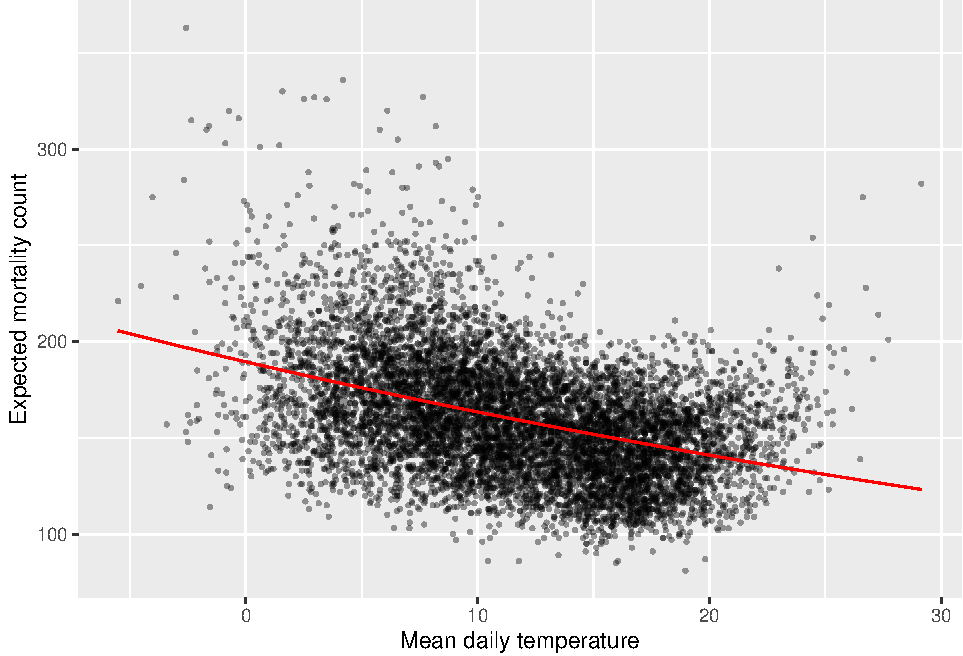
\includegraphics{adv_epi_analysis_files/figure-latex/unnamed-chunk-33-1.pdf}

For this model, we can interpret the coefficient for the temperature covariate
as the expected log relative risk in the health outcome associated with a
one-unit increase in temperature. We can exponentiate this value to get an
estimate of the relative risk:

\begin{Shaded}
\begin{Highlighting}[]
\CommentTok{\# Extract the temperature coefficient from the model}
\NormalTok{tmean\_coef }\OtherTok{\textless{}{-}}\NormalTok{ mod\_pois\_reg }\SpecialCharTok{\%\textgreater{}\%} 
  \FunctionTok{tidy}\NormalTok{() }\SpecialCharTok{\%\textgreater{}\%} 
  \FunctionTok{filter}\NormalTok{(term }\SpecialCharTok{==} \StringTok{"tmean"}\NormalTok{) }\SpecialCharTok{\%\textgreater{}\%} \CommentTok{\# Extract the row with the tmean estimates}
  \FunctionTok{pull}\NormalTok{(estimate) }\CommentTok{\# Extract just the point estimate}

\CommentTok{\# Estimate of the log relative risk for a one{-}unit increase in temperature}
\NormalTok{tmean\_coef }
\end{Highlighting}
\end{Shaded}

\begin{verbatim}
## [1] -0.0147728
\end{verbatim}

\begin{Shaded}
\begin{Highlighting}[]
\CommentTok{\# Estimate of the relative risk for a one{-}unit increase in temperature}
\FunctionTok{exp}\NormalTok{(tmean\_coef)}
\end{Highlighting}
\end{Shaded}

\begin{verbatim}
## [1] 0.9853358
\end{verbatim}

If you want to estimate the confidence interval for this estimate, you should
calculate that \emph{before} exponentiating.

\begin{enumerate}
\def\labelenumi{\arabic{enumi}.}
\setcounter{enumi}{2}
\tightlist
\item
  \textbf{Change your function call to allow for overdispersion in the outcome data
  (daily mortality count). How does the estimated coefficient for temperature
  change between the model fit for \#2 and this model? Check both the central
  estimate and its estimated standard error.}
\end{enumerate}

In the R \texttt{glm} call, there is a family that is similar to Poisson (including
using a log link), but that allows for overdispersion. You can specify it
with the ``quasipoisson'' choice for the \texttt{family} parameter in the \texttt{glm} call:

\begin{Shaded}
\begin{Highlighting}[]
\NormalTok{mod\_ovdisp\_reg }\OtherTok{\textless{}{-}} \FunctionTok{glm}\NormalTok{(all }\SpecialCharTok{\textasciitilde{}}\NormalTok{ tmean, }\AttributeTok{data =}\NormalTok{ obs, }\AttributeTok{family =} \StringTok{"quasipoisson"}\NormalTok{)}
\end{Highlighting}
\end{Shaded}

When you use this family, there will be some new information in the summary
for the model object. It will now include a dispersion parameter (\(\phi\)). If this
is close to 1, then the data were close to the assumed variance for a Poisson
distribution (i.e., there was little evidence of overdispersion). In the
example, the overdispersion is around 5, suggesting the data are overdispersed
(this might come down some when we start including independent variables that
explain some of the variation in the outcome variable, like long-term and
seasonal trends).

\begin{Shaded}
\begin{Highlighting}[]
\FunctionTok{summary}\NormalTok{(mod\_ovdisp\_reg)}
\end{Highlighting}
\end{Shaded}

\begin{verbatim}
## 
## Call:
## glm(formula = all ~ tmean, family = "quasipoisson", data = obs)
## 
## Coefficients:
##               Estimate Std. Error t value Pr(>|t|)    
## (Intercept)  5.2445409  0.0044087  1189.6   <2e-16 ***
## tmean       -0.0147728  0.0003543   -41.7   <2e-16 ***
## ---
## Signif. codes:  0 '***' 0.001 '**' 0.01 '*' 0.05 '.' 0.1 ' ' 1
## 
## (Dispersion parameter for quasipoisson family taken to be 5.006304)
## 
##     Null deviance: 49297  on 8278  degrees of freedom
## Residual deviance: 40587  on 8277  degrees of freedom
## AIC: NA
## 
## Number of Fisher Scoring iterations: 4
\end{verbatim}

If you compare the estimates of the temperature coefficient from the Poisson
regression with those when you allow for overdispersion, you'll see something
interesting:

\begin{Shaded}
\begin{Highlighting}[]
\FunctionTok{tidy}\NormalTok{(mod\_pois\_reg) }\SpecialCharTok{\%\textgreater{}\%} 
  \FunctionTok{filter}\NormalTok{(term }\SpecialCharTok{==} \StringTok{"tmean"}\NormalTok{)}
\end{Highlighting}
\end{Shaded}

\begin{verbatim}
## # A tibble: 1 x 5
##   term  estimate std.error statistic p.value
##   <chr>    <dbl>     <dbl>     <dbl>   <dbl>
## 1 tmean  -0.0148  0.000158     -93.3       0
\end{verbatim}

\begin{Shaded}
\begin{Highlighting}[]
\FunctionTok{tidy}\NormalTok{(mod\_ovdisp\_reg) }\SpecialCharTok{\%\textgreater{}\%} 
  \FunctionTok{filter}\NormalTok{(term }\SpecialCharTok{==} \StringTok{"tmean"}\NormalTok{)}
\end{Highlighting}
\end{Shaded}

\begin{verbatim}
## # A tibble: 1 x 5
##   term  estimate std.error statistic p.value
##   <chr>    <dbl>     <dbl>     <dbl>   <dbl>
## 1 tmean  -0.0148  0.000354     -41.7       0
\end{verbatim}

The central estimate (\texttt{estimate} column) is very similar. However, the estimated
standard error is larger when the model allows for overdispersion. This
indicates that the Poisson model was too simple, and that its inherent
assumption that data were not overdispersed was problematic. If you naively used
a Poisson regression in this case, then you would estimate a confidence
interval on the temperature coefficient that would be too narrow. This could
cause you to conclude that the estimate was statistically significant when
you should not have (although in this case, the estimate is statistically
significant under both models).

\begin{enumerate}
\def\labelenumi{\arabic{enumi}.}
\setcounter{enumi}{3}
\tightlist
\item
  \textbf{Change your function call to include control for day of week.}
\end{enumerate}

Day of week is included in the data as a categorical variable, using a
data type in R called a factor. You are now essentially fitting this model:

\(log(Y)=\beta_{0}+\beta_{1}X1+\gamma^{'}X2\),

where \(X2\) is a categorical variable for day of the week and \(\gamma^{'}\)
represents a vector of parameters associated with each category.

It is pretty straightforward to include factors as independent variables in calls
to \texttt{glm}: you just add the column name to the list of other independent variables
with a \texttt{+}. In this case, we need to do one more step: earlier, we added order to
\texttt{dow}, so it would ``remember'' the order of the week days (Monday before Tuesday,
etc.). However, we need to strip off this order before we include the factor in
the \texttt{glm} call. One way to do this is with the \texttt{factor} call, specifying
\texttt{ordered\ =\ FALSE}. Here is the full call to fit this model:

\begin{Shaded}
\begin{Highlighting}[]
\NormalTok{mod\_ctrl\_dow }\OtherTok{\textless{}{-}} \FunctionTok{glm}\NormalTok{(all }\SpecialCharTok{\textasciitilde{}}\NormalTok{ tmean }\SpecialCharTok{+} \FunctionTok{factor}\NormalTok{(dow, }\AttributeTok{ordered =} \ConstantTok{FALSE}\NormalTok{), }
                    \AttributeTok{data =}\NormalTok{ obs, }\AttributeTok{family =} \StringTok{"quasipoisson"}\NormalTok{)}
\end{Highlighting}
\end{Shaded}

When you look at the summary for the model object, you can see that the
model has fit a separate model parameter for six of the seven weekdays. The one
weekday that isn't fit (Sunday in this case) serves as a baseline ---these
estimates specify how the log of the expected mortality count is expected to
differ on, for example, Monday versus Sunday (by about 0.03), if the temperature
is the same for the two days.

\begin{Shaded}
\begin{Highlighting}[]
\FunctionTok{summary}\NormalTok{(mod\_ctrl\_dow)}
\end{Highlighting}
\end{Shaded}

\begin{verbatim}
## 
## Call:
## glm(formula = all ~ tmean + factor(dow, ordered = FALSE), family = "quasipoisson", 
##     data = obs)
## 
## Coefficients:
##                                   Estimate Std. Error t value Pr(>|t|)    
## (Intercept)                      5.2208502  0.0065277 799.804  < 2e-16 ***
## tmean                           -0.0147723  0.0003538 -41.750  < 2e-16 ***
## factor(dow, ordered = FALSE)Mon  0.0299282  0.0072910   4.105 4.08e-05 ***
## factor(dow, ordered = FALSE)Tue  0.0292575  0.0072920   4.012 6.07e-05 ***
## factor(dow, ordered = FALSE)Wed  0.0255224  0.0073020   3.495 0.000476 ***
## factor(dow, ordered = FALSE)Thu  0.0269580  0.0072985   3.694 0.000222 ***
## factor(dow, ordered = FALSE)Fri  0.0355431  0.0072834   4.880 1.08e-06 ***
## factor(dow, ordered = FALSE)Sat  0.0181489  0.0073158   2.481 0.013129 *  
## ---
## Signif. codes:  0 '***' 0.001 '**' 0.01 '*' 0.05 '.' 0.1 ' ' 1
## 
## (Dispersion parameter for quasipoisson family taken to be 4.992004)
## 
##     Null deviance: 49297  on 8278  degrees of freedom
## Residual deviance: 40434  on 8271  degrees of freedom
## AIC: NA
## 
## Number of Fisher Scoring iterations: 4
\end{verbatim}

You can also see from this summary that the coefficients for the day of the
week are all statistically significant. Even though we didn't see a big
difference in mortality counts by day of week in our exploratory analysis,
this suggests that it does help explain some variance in mortality observations
and will likely be worth including in the final model.

The model now includes day of week when fitting an expected mortality count
for each observation. As a result, if you plot fitted values of expected
mortality versus mean daily temperature, you'll see some ``hoppiness'' in the
fitted line:

\begin{Shaded}
\begin{Highlighting}[]
\NormalTok{mod\_ctrl\_dow }\SpecialCharTok{\%\textgreater{}\%} 
  \FunctionTok{augment}\NormalTok{() }\SpecialCharTok{\%\textgreater{}\%} 
  \FunctionTok{ggplot}\NormalTok{(}\FunctionTok{aes}\NormalTok{(}\AttributeTok{x =}\NormalTok{ tmean)) }\SpecialCharTok{+} 
  \FunctionTok{geom\_point}\NormalTok{(}\FunctionTok{aes}\NormalTok{(}\AttributeTok{y =}\NormalTok{ all), }\AttributeTok{alpha =} \FloatTok{0.4}\NormalTok{, }\AttributeTok{size =} \FloatTok{0.5}\NormalTok{) }\SpecialCharTok{+} 
  \FunctionTok{geom\_line}\NormalTok{(}\FunctionTok{aes}\NormalTok{(}\AttributeTok{y =} \FunctionTok{exp}\NormalTok{(.fitted)), }\AttributeTok{color =} \StringTok{"red"}\NormalTok{) }\SpecialCharTok{+} 
  \FunctionTok{labs}\NormalTok{(}\AttributeTok{x =} \StringTok{"Mean daily temperature"}\NormalTok{, }\AttributeTok{y =} \StringTok{"Expected mortality count"}\NormalTok{)}
\end{Highlighting}
\end{Shaded}

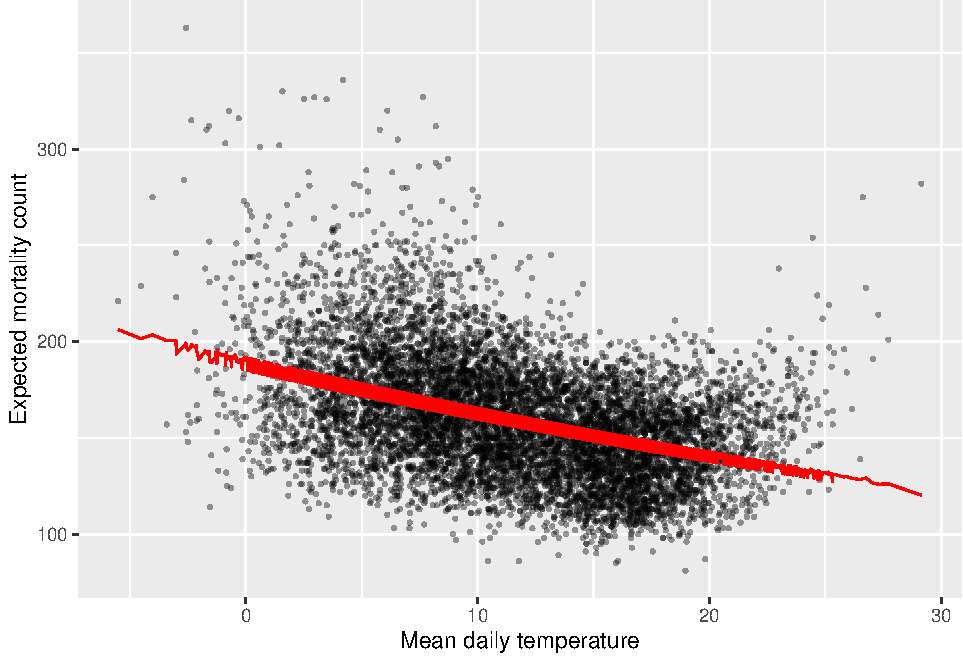
\includegraphics{adv_epi_analysis_files/figure-latex/unnamed-chunk-40-1.pdf}

This is because each fitted value is also incorporating the expected influence
of day of week on the mortality count, and that varies across the observations
(i.e., you could have two days with the same temperature, but different
expected mortality from the model, because they occur on different days).

If you plot the model fits separately for each day of the week, you'll see that
the line is smooth across all observations from the same day of the week:

\begin{Shaded}
\begin{Highlighting}[]
\NormalTok{mod\_ctrl\_dow }\SpecialCharTok{\%\textgreater{}\%} 
  \FunctionTok{augment}\NormalTok{() }\SpecialCharTok{\%\textgreater{}\%} 
  \FunctionTok{ggplot}\NormalTok{(}\FunctionTok{aes}\NormalTok{(}\AttributeTok{x =}\NormalTok{ tmean)) }\SpecialCharTok{+} 
  \FunctionTok{geom\_point}\NormalTok{(}\FunctionTok{aes}\NormalTok{(}\AttributeTok{y =}\NormalTok{ all), }\AttributeTok{alpha =} \FloatTok{0.4}\NormalTok{, }\AttributeTok{size =} \FloatTok{0.5}\NormalTok{) }\SpecialCharTok{+} 
  \FunctionTok{geom\_line}\NormalTok{(}\FunctionTok{aes}\NormalTok{(}\AttributeTok{y =} \FunctionTok{exp}\NormalTok{(.fitted)), }\AttributeTok{color =} \StringTok{"red"}\NormalTok{) }\SpecialCharTok{+} 
  \FunctionTok{labs}\NormalTok{(}\AttributeTok{x =} \StringTok{"Mean daily temperature"}\NormalTok{, }\AttributeTok{y =} \StringTok{"Expected mortality count"}\NormalTok{) }\SpecialCharTok{+} 
  \FunctionTok{facet\_wrap}\NormalTok{(}\SpecialCharTok{\textasciitilde{}}\NormalTok{ obs}\SpecialCharTok{$}\NormalTok{dow)}
\end{Highlighting}
\end{Shaded}

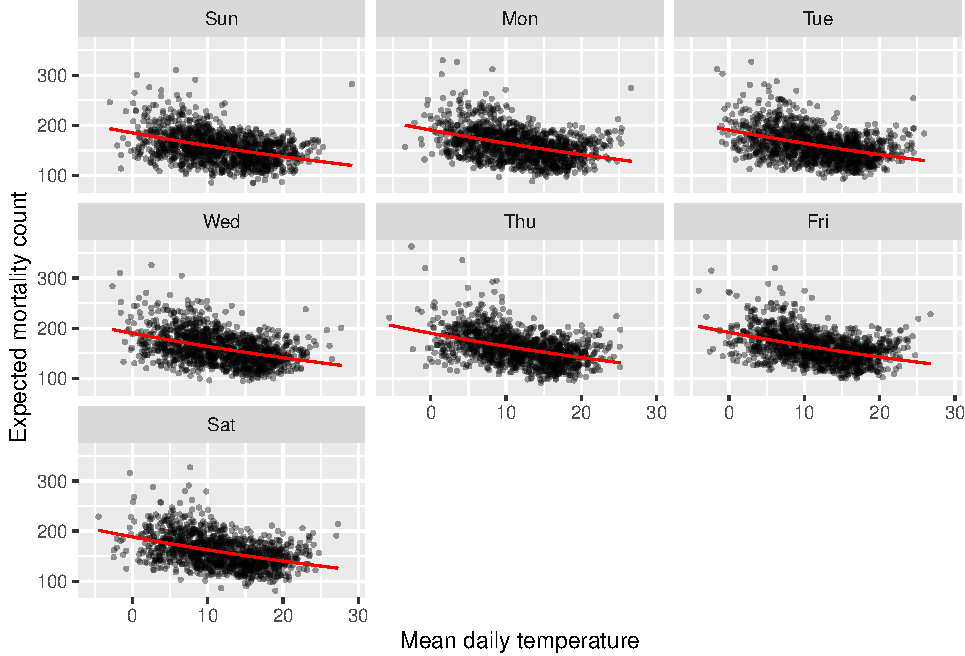
\includegraphics{adv_epi_analysis_files/figure-latex/unnamed-chunk-41-1.pdf}

\emph{Wrapping up}

At this point, the coefficient estimates suggests that risk of mortality
tends to decrease as temperature increases. Do you think this is reasonable?
What else might be important to build into the model based on your analysis
up to this point?

\chapter{Generalized linear models}\label{generalized-linear-models}

\section{Readings}\label{readings-1}

The readings for this chapter are:

\begin{itemize}
\tightlist
\item
  \citet{bhaskaran2013time} Provides an overview of time series regression
  in environmental epidemiology.
\item
  \citet{vicedo2019hands} Provides a tutorial of all the steps for a
  projecting of health impacts of temperature extremes under climate change.
  One of the steps is to fit the exposure-response association using present-day data
  (the section on ``Estimation of Exposure-Response Associations'' in the paper).
  In this chapter, we will go into details on that step, and that section of the paper
  is the only required reading for this chapter. Later in the class, we'll
  look at other steps covered in this paper. Supplemental material for this paper is
  available to download by
  clicking \url{http://links.lww.com/EDE/B504}. You will need the data in this supplement
  for the exercises for class.
\item
  \citet{armstrong2014conditional} This paper describes different data structures for
  case-crossover data, as well as how conditional Poisson regression can be used
  in some cases to fit a statistical model to these data.
  Supplemental material for this paper is available at
  \url{https://bmcmedresmethodol.biomedcentral.com/articles/10.1186/1471-2288-14-122\#Sec13}.
\end{itemize}

The following are supplemental readings (i.e., not required, but may be of
interest) associated with the material in this chapter:

\begin{itemize}
\tightlist
\item
  \citet{armstrong2006models} Covers similar material as \citet{bhaskaran2013time}, but with
  more focus on the statistical modeling framework (highly recommended!)
\item
  \citet{gasparrini2010time} Describes some of the advances made to time series study
  designs and statistical analysis, specifically in the context of temperature
\item
  \citet{basu2005temperature} Compares time series and case-crossover study designs in
  the context of exploring temperature and health. Includes a nice illustration
  of different referent periods, including time-stratified.
\item
  \citet{imai2015time} Typically, the time series study design covered in this
  chapter is used to study non-communicable health outcomes. This paper discusses
  opportunities and limitations in applying a similar framework for infectious
  disease.
\item
  \citet{lu2007equivalence} Heavier on statistics. This paper shows how, under
  conditions often common for environmental epidemiology studies, case-crossover
  and time series methods are equivalent.
\item
  \citet{gasparrini2014modeling} Heavier on statistics. This provides the statistical
  framework for the distributed lag model for environmental epidemiology time
  series studies.
\item
  \citet{dunn2018generalized1} Introduction to statistical models, moving into regression models and
  generalized linear models. Chapter in a book that is available online through the CSU library.
\item
  \citet{james2013introduction3} General overview of linear regression, with an R coding
  ``lab'' at the end to provide coding examples. Covers model fit, continuous, binary,
  and categorical covariates, and interaction terms. Chapter in a book that is
  available online through the CSU library.
\end{itemize}

\section{Splines in GLMs}\label{splines-in-glms}

We saw from the last model, with a linear term for mean daily temperature, that the
suggested effect on mortality is a decrease in daily mortality counts with
increasing temperature. However, as you've probably guessed that's likely not
entirely accurate. A linear term for the effect of exposure restricts us to an
effect that can be fitted with a straight line (either a null effect or a
monotonically increasing or decreasing effect with increasing exposure).

This clearly is problematic in some cases. One example is when exploring the
association between temperature and health risk. Based on human physiology,
we would expect many health risks to be elevated at temperature extremes,
whether those are extreme cold or extreme heat. A linear term would be
inadequate to describe this kind of U-shaped association. Other effects might
have a threshold---for example, heat stroke might have a very low risk at
most temperatures, only increasing with temperature above a certain threshold.

We can
capture non-linear patterns in effects, by using different functions of X.
Examples are \(\sqrt{X}\), \(X^{2}\), or more complex smoothing functions, such as
polynomials or splines. Polynomials might at first make a lot of sense,
especially since you've likely come across polynomial terms in mathematics
classes since grade school. However, it turns out that they have some undesirable
properties. A key one is that they can have extreme behavior, particularly
when using a high-order polynomial, and particularly outside the range of
data that are available to fit the model.

An alternative that is generally preferred for environmental epidemiology
studies is the regression spline. The word ``spline'' originally comes from
drafting and engineering (ship building, in particular), where it described
a flexible piece of wood or metal that you could use to draw a curved line---it created
a curve that was flexible enough---but just flexible enough---to fit a space
(see Wikipedia's very interesting article on \href{https://en.wikipedia.org/wiki/Flat_spline}{flat splines} for more).

Splines follow a similar idea in mathematics, making them helpful tools when
a line won't fit your data well. In general, a spline fits together a few
simpler functions to create something with a curve or non-linearity. Each
simpler function operates within an interval of the data, and then they join
together at ``knots'' along the range of the data.
Regression splines are therefore simple parametric smoothing function,
which fit separate polynomial in each interval of the range of the predictor; these
can be linear, quadratic, and cubic.

The simplest example is a linear spline (also called a piecewise linear function).
This type of spline creates non-linearity by having
a breakpoint at the knot, allowing the slope of the line to be different in
the intervals of data on either side of the knot. The following plot shows an
example. Say you want to explore how mean temperature varies by the day in the
year (Jan 1 = 1, Jan 2 = 2, and so on) in the London example dataset from the
last chapter. Temperature tends to increase with day of
year for a while, but then it changes around the start of August, after that
decreasing with day of year. This patterns means that a line will give a bad fit
for how temperature changes with day of year, since it smooths right through that
change. On the other hand, you can get a very reasonable fit using a linear spline
with a knot around August 1 (day 213 in the year). These two examples are shown in
the following plot, with the linear function fit on the left and the linear spline
on the right:

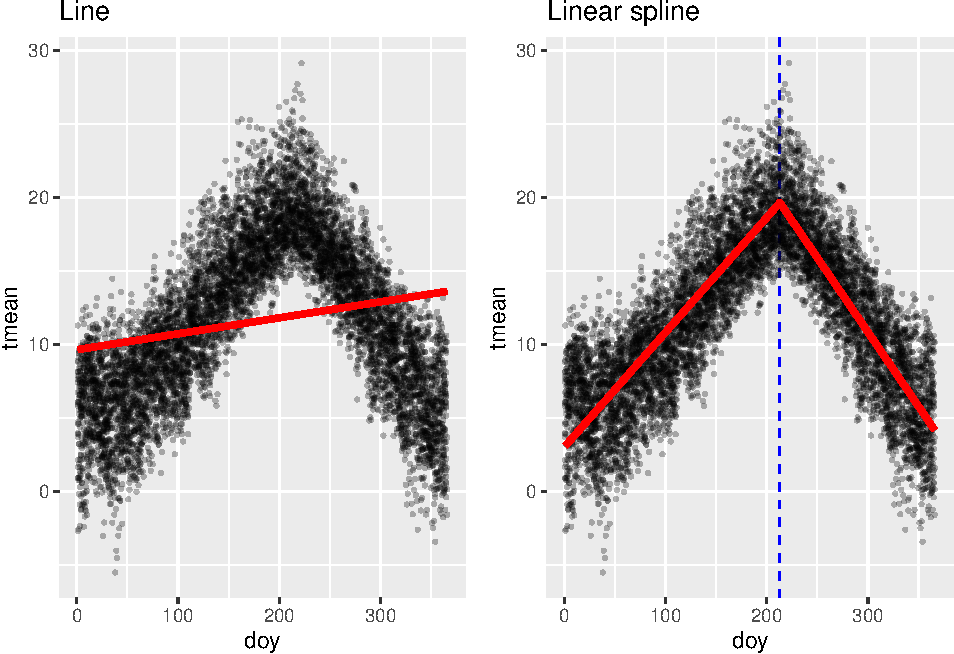
\includegraphics{adv_epi_analysis_files/figure-latex/unnamed-chunk-42-1.pdf}

If you were to write out these regression models in mathematical notation, the
linear one is very simple:

\[
Y_t = \alpha + \beta X_t
\]
where \(Y_t\) is the temperature on day \(t\), \(\alpha\) is the model intercept,
\(X_t\) is the day of the year on day \(t\), and \(\beta\) is the estimated coefficient
for \(X_t\).

The notation for the model with the linear spline is a bit more complex:

\[
Y_t = \alpha + \beta_1 X_t + \beta_2 (X_t - k)_+
\]

Here, \(Y_t\) is again the temperature on day \(t\), \(X_t\) is again the day of the year
on day \(t\), and \(\alpha\) is again the intercept. The term \(k\) is the ``knot''---the
value of \(X\) where we're letting the slope change. In this example, we're using
\(k = 213\). The term \((X_t - k)_+\) has a special meaning---it takes the value
0 if \(X_t\) is in the interval to the left of the knot, while if \(X_t\) is in the
interval to the right of the knot, it takes the value of \(X_t\) minus the knot
value:

\[ 
(X_t - k)_+ =
\begin{cases}
0, & \mbox{if } X_t < k \\
X_t - k, & \mbox{if } X_t \ge k 
\end{cases}
\]

In this model, the coefficient \(\beta_1\) estimates the slope of the line to the
left of the knot, while \(\beta_2\) estimates how that slope will change to the
right of the knot.

Fortunately, we usually won't have to get this complex in the model notation,
especially when we use more complex splines (where the notation would get even
more complex). Instead, we'll often write out the
regression equation in a simpler way, just indicating that we're using a function
of the covariate, rather than the covariate directly:

\[
Y_t = \alpha + f(X_t | \mathbf{\beta})
\]

where we can note that \(f(X_t)\) is a function of day of the year (\(X_t\)), fit in
this case using a linear spline, and with a set of estimated coefficients \(\mathbf{\beta}\) for that
function (see \citet{armstrong2006models} for an example of using this model notation).

While a linear spline is the simplest conceptually (and mathematically), it often
isn't very satisfying, because it fits a function with a sharp breakpoint, which
often isn't realistic. For example, the linear spline fit above suggests that the
relationship between day of the year and temperature changes abruptly and dramatically
on August 1 of the year. In reality, we know that this change in the relationship
between day of year and temperature is probably a lot smoother.

To fit smoother shapes, we can move to higher level splines. Cubic splines
(``cubic'' because they include terms of the covariate up to the third power) are
very popular.
An example of a cubic spline
function is \(X+X^{2}+X^{3}+I((X>X_{0})*(X-X_{0})^3)\). This particular function is
a cubic spline with four degrees of freedom (\(df=4\)) and one knot (\(X_{0}\)).
A special type of cubic spline called a natural cubic spline is particularly popular.
Unlike a polynomial function, a natural cubic spline ``behaves'' better outside
the range of the data used to fit the model---they are constrained to continue
on a linear trajectory once they pass beyond the range of the data.

Regression splines can be fit in a GLM via the package \texttt{splines}. Two commonly
used examples of regression splines are b-splines and natural cubic
splines. \citet{vicedo2019hands} uses natural cubic splines, which can be fit with the
\texttt{ns} (for ``natural spline'') function from the \texttt{splines} package.

While splines are great for fitting non-linear relationships, they do create some
challenges in interpreting the results. When you fit a linear relationship for
a covariate, you will get a single estimate that helps describe the fitted relationship
between that covariate and the outcome variable. However, when you use a non-linear
function, you'll end up with a mix of coefficients associated with that function.
Sometimes, you will use splines to control for a potential confounder (as we
will in the exercises for this first part of the chapter). In this case, you don't
need to worry about interpreting the estimated coefficients---you're just trying to
control for the variable, rather than inferring anything about how it's associated
with the outcome.
In later parts of this chapter, we'll talk about how to interpret these coefficients
if you're using a spline for the exposure that you're interested in, when we talk
more broadly about basis functions.

\emph{Applied: Including a spline in a GLM}

For this exercise, you will continue to build up the model that you began in
the examples in the previous chapter. The example uses the data provided with
one of this chapter's readings, \citet{vicedo2019hands}.

\begin{enumerate}
\def\labelenumi{\arabic{enumi}.}
\tightlist
\item
  Start by fitting a somewhat simple model---how are daily mortality counts
  associated with (a) a linear and (b) a non-linear function of time? Is a linear
  term appropriate to describe this association? What types of patterns are
  captured by a non-linear function that are missed by a linear function?
\item
  In the last chapter, the final version of the model used a GLM with an
  overdispersed Poisson distribution, including control for day of week.
  Start from this model and add control for long-term and seasonal trends
  over the study period.
\item
  Refine your model to fit for a non-linear, rather than linear, function
  of temperature in the model. Does a non-linear term seem to be more
  appropriate than a linear term?
\end{enumerate}

\emph{Applied exercise: Example code}

\begin{enumerate}
\def\labelenumi{\arabic{enumi}.}
\tightlist
\item
  \textbf{Start by fitting a somewhat simple model---how are daily mortality counts
  associated with (a) a linear and (b) a non-linear function of time?}
\end{enumerate}

It is helpful to start by loading the R packages you are likely to need, as
well as the example dataset. You may also need to re-load the example data
and perform the steps taken to clean it in the last chapter:

\begin{Shaded}
\begin{Highlighting}[]
\CommentTok{\# Load some packages that will likely be useful}
\FunctionTok{library}\NormalTok{(tidyverse)}
\FunctionTok{library}\NormalTok{(viridis)}
\FunctionTok{library}\NormalTok{(lubridate)}
\FunctionTok{library}\NormalTok{(broom)}

\CommentTok{\# Load and clean the data}
\NormalTok{obs }\OtherTok{\textless{}{-}} \FunctionTok{read\_csv}\NormalTok{(}\StringTok{"data/lndn\_obs.csv"}\NormalTok{) }\SpecialCharTok{\%\textgreater{}\%} 
  \FunctionTok{mutate}\NormalTok{(}\AttributeTok{dow =} \FunctionTok{wday}\NormalTok{(date, }\AttributeTok{label =} \ConstantTok{TRUE}\NormalTok{))}
\end{Highlighting}
\end{Shaded}

For this first question, the aim is to model the association between time and
daily mortality counts within the example data. This approach is often used
to explore and, if needed, adjust for temporal factors in the data.

There are a number of factors that can act over time to create patterns in both
environmental exposures and health outcomes. For example, there may be changes
in air pollution exposures over the years of a study because of changes in
regulations or growth or decline of factories and automobile traffic in an area.
Changes in health care and in population demographics can cause patterns in
health outcomes over the study period. At a shorter, seasonal term, there are
also factors that could influence both exposures and outcomes, including
seasonal changes in climate, seasonal changes in emissions, and seasonal
patterns in health outcomes.

It can be difficult to pinpoint and measure these temporal factors, and so
instead a common practice is to include model control based on the time in the
study. This can be measured, for example, as the day since the start of the
study period.

You can easily add a column for day in study for a dataset that
includes date. R saves dates in a special format, which we're using the in
\texttt{obs} dataset:

\begin{Shaded}
\begin{Highlighting}[]
\FunctionTok{class}\NormalTok{(obs}\SpecialCharTok{$}\NormalTok{date)}
\end{Highlighting}
\end{Shaded}

\begin{verbatim}
## [1] "Date"
\end{verbatim}

However, this is just a fancy overlay on a value that's ultimately saved as
a number. Like most Unix programs, the date is saved as the number of days
since the Unix ``epoch'', January 1, 1970. You can take advantage of this
convention---if you use \texttt{as.numeric} around a date in R, it will give you a
number that gets one unit higher for every new date. Here's the example for
the first date in our example data:

\begin{Shaded}
\begin{Highlighting}[]
\NormalTok{obs}\SpecialCharTok{$}\NormalTok{date[}\DecValTok{1}\NormalTok{]}
\end{Highlighting}
\end{Shaded}

\begin{verbatim}
## [1] "1990-01-01"
\end{verbatim}

\begin{Shaded}
\begin{Highlighting}[]
\FunctionTok{as.numeric}\NormalTok{(obs}\SpecialCharTok{$}\NormalTok{date[}\DecValTok{1}\NormalTok{]) }
\end{Highlighting}
\end{Shaded}

\begin{verbatim}
## [1] 7305
\end{verbatim}

And here's the example for the next date:

\begin{Shaded}
\begin{Highlighting}[]
\NormalTok{obs}\SpecialCharTok{$}\NormalTok{date[}\DecValTok{2}\NormalTok{]}
\end{Highlighting}
\end{Shaded}

\begin{verbatim}
## [1] "1990-01-02"
\end{verbatim}

\begin{Shaded}
\begin{Highlighting}[]
\FunctionTok{as.numeric}\NormalTok{(obs}\SpecialCharTok{$}\NormalTok{date[}\DecValTok{2}\NormalTok{])}
\end{Highlighting}
\end{Shaded}

\begin{verbatim}
## [1] 7306
\end{verbatim}

You can use this convention to add a column that gives days since the first
study date. While you could also use the \texttt{1:n()} call to get a number for
each row that goes from 1 to the number of rows, that approach would not
catch any ``skips'' in dates in the data (e.g., missing dates if only warm-season
data are included). The use of the dates is more robust:

\begin{Shaded}
\begin{Highlighting}[]
\NormalTok{obs }\OtherTok{\textless{}{-}}\NormalTok{ obs }\SpecialCharTok{\%\textgreater{}\%} 
  \FunctionTok{mutate}\NormalTok{(}\AttributeTok{time =} \FunctionTok{as.numeric}\NormalTok{(date) }\SpecialCharTok{{-}} \FunctionTok{first}\NormalTok{(}\FunctionTok{as.numeric}\NormalTok{(date)))}

\NormalTok{obs }\SpecialCharTok{\%\textgreater{}\%} 
  \FunctionTok{select}\NormalTok{(date, time)}
\end{Highlighting}
\end{Shaded}

\begin{verbatim}
## # A tibble: 8,279 x 2
##    date        time
##    <date>     <dbl>
##  1 1990-01-01     0
##  2 1990-01-02     1
##  3 1990-01-03     2
##  4 1990-01-04     3
##  5 1990-01-05     4
##  6 1990-01-06     5
##  7 1990-01-07     6
##  8 1990-01-08     7
##  9 1990-01-09     8
## 10 1990-01-10     9
## # i 8,269 more rows
\end{verbatim}

As a next step, it is always useful to use exploratory data analysis to look
at the patterns that might exist for an association, before you start designing
and fitting the regression model.

\begin{Shaded}
\begin{Highlighting}[]
\FunctionTok{ggplot}\NormalTok{(obs, }
       \FunctionTok{aes}\NormalTok{(}\AttributeTok{x =}\NormalTok{ time, }\AttributeTok{y =}\NormalTok{ all)) }\SpecialCharTok{+}
  \FunctionTok{geom\_point}\NormalTok{(}\AttributeTok{size =} \FloatTok{0.5}\NormalTok{, }\AttributeTok{alpha =} \FloatTok{0.5}\NormalTok{)}
\end{Highlighting}
\end{Shaded}

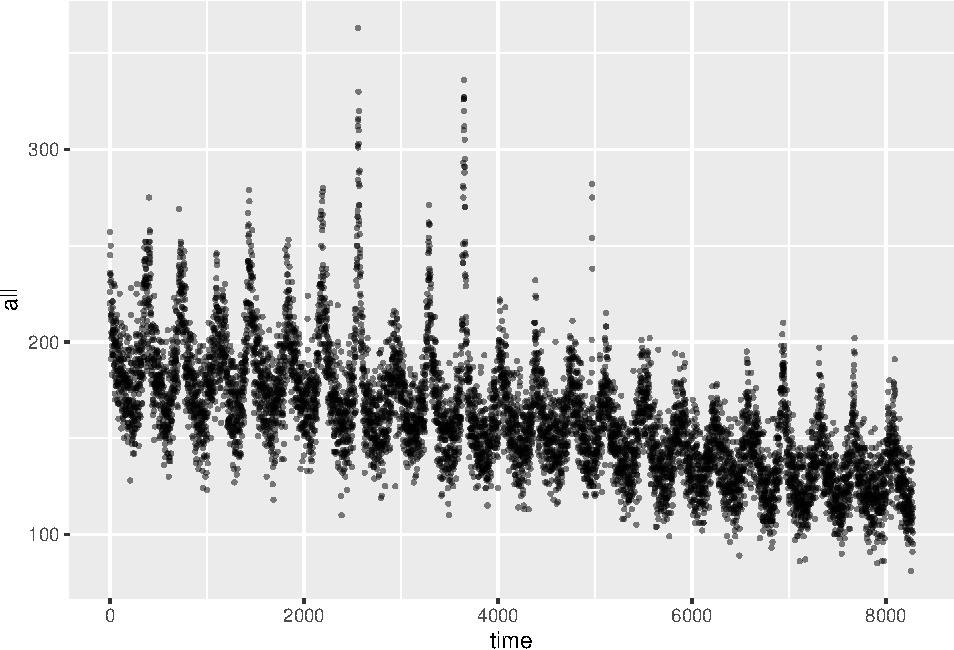
\includegraphics{adv_epi_analysis_files/figure-latex/unnamed-chunk-48-1.pdf}

There are clear patterns between time and daily mortality counts in these data.
First, there is a clear long-term pattern, with mortality rates declining on
average over time. Second, there are clear seasonal patterns, with higher
mortality generally in the winter and lower rates in the summer.

To model this, we can start with fitting a linear term. In the last chapter,
we determined that the mortality outcome data can be fit using a GLM with a
Poisson family, allowing for overdispersion as it is common in real-life
count data like these. To include time as a linear term, we can just include
that column name to the right of the \texttt{\textasciitilde{}} in the model formula:

\begin{Shaded}
\begin{Highlighting}[]
\NormalTok{mod\_time }\OtherTok{\textless{}{-}} \FunctionTok{glm}\NormalTok{(all }\SpecialCharTok{\textasciitilde{}}\NormalTok{ time, }
                \AttributeTok{data =}\NormalTok{ obs, }\AttributeTok{family =} \StringTok{"quasipoisson"}\NormalTok{)}
\end{Highlighting}
\end{Shaded}

You can use the \texttt{augment} function from the \texttt{broom} package to pull out the
fitted estimate for each of the original observations and plot that, along
with the observed data, to get an idea of what this model has captured:

\begin{Shaded}
\begin{Highlighting}[]
\NormalTok{mod\_time }\SpecialCharTok{\%\textgreater{}\%} 
  \FunctionTok{augment}\NormalTok{() }\SpecialCharTok{\%\textgreater{}\%} 
  \FunctionTok{ggplot}\NormalTok{(}\FunctionTok{aes}\NormalTok{(}\AttributeTok{x =}\NormalTok{ time)) }\SpecialCharTok{+} 
  \FunctionTok{geom\_point}\NormalTok{(}\FunctionTok{aes}\NormalTok{(}\AttributeTok{y =}\NormalTok{ all), }\AttributeTok{alpha =} \FloatTok{0.4}\NormalTok{, }\AttributeTok{size =} \FloatTok{0.5}\NormalTok{) }\SpecialCharTok{+} 
  \FunctionTok{geom\_line}\NormalTok{(}\FunctionTok{aes}\NormalTok{(}\AttributeTok{y =} \FunctionTok{exp}\NormalTok{(.fitted)), }\AttributeTok{color =} \StringTok{"red"}\NormalTok{) }\SpecialCharTok{+} 
  \FunctionTok{labs}\NormalTok{(}\AttributeTok{x =} \StringTok{"Date in study"}\NormalTok{, }\AttributeTok{y =} \StringTok{"Expected mortality count"}\NormalTok{) }
\end{Highlighting}
\end{Shaded}

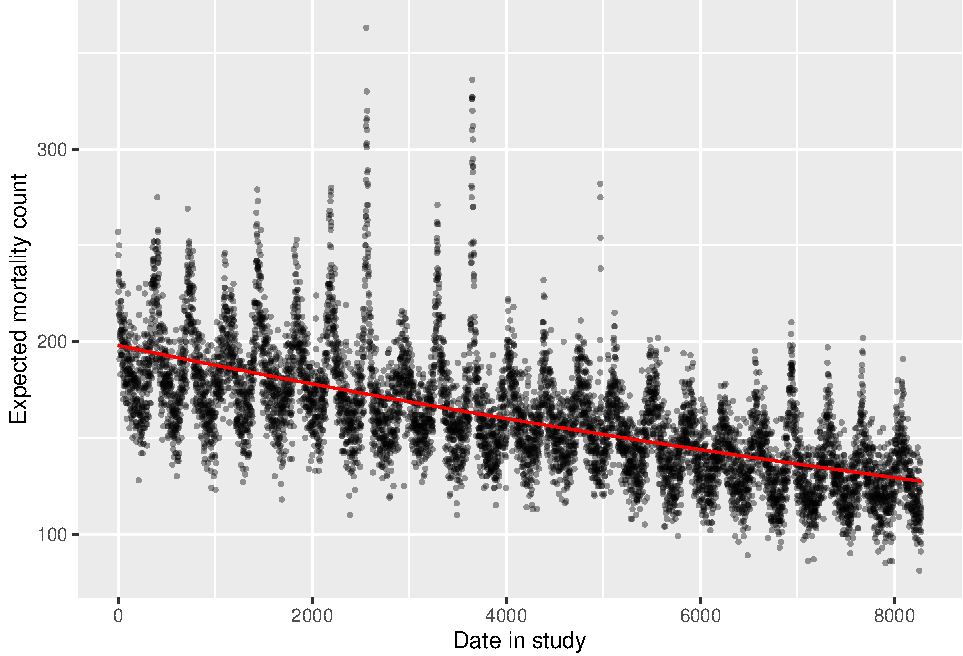
\includegraphics{adv_epi_analysis_files/figure-latex/unnamed-chunk-50-1.pdf}

This linear trend captures the long-term trend in mortality rates fairly well in
this case. This won't always be the case, as there may be some health
outcomes---or some study populations---where the long-term pattern over the
study period might be less linear than in this example. Further, the linear
term is completely unsuccessful in capturing the shorter-term trends in mortality
rate. These oscillate, and so would be impossible to capture over multiple
years with a linear trend.

Instead, it's helpful to use a non-linear term for time in the model. We can
use a natural cubic spline for this, using the \texttt{ns} function from the \texttt{splines}
package. You will need to clarify how flexible the spline function should be,
and this can be specified through the degrees of freedom for the spline. A
spline with more degrees of freedom will be ``wigglier'' over a given data range
compared to a spline with fewer degrees of freedom. Let's start by using
158 degrees of freedom, which translates to about 7 degrees of freedom per year:

\begin{Shaded}
\begin{Highlighting}[]
\FunctionTok{library}\NormalTok{(splines)}
\NormalTok{mod\_time\_nonlin }\OtherTok{\textless{}{-}} \FunctionTok{glm}\NormalTok{(all }\SpecialCharTok{\textasciitilde{}} \FunctionTok{ns}\NormalTok{(time, }\AttributeTok{df =} \DecValTok{158}\NormalTok{), }
                       \AttributeTok{data =}\NormalTok{ obs, }\AttributeTok{family =} \StringTok{"quasipoisson"}\NormalTok{)}
\end{Highlighting}
\end{Shaded}

You can visualize the model results in a similar way to how we visualized the
last model. However, there is one extra step. The \texttt{augment} function only
carries through columns in the original data (\texttt{obs}) that were directly used
in fitting the model. Now that we're using a transformation of the \texttt{time}
column, by wrapping it in \texttt{ns}, the \texttt{time} column is no longer included in the
\texttt{augment} output. However, we can easily add it back in using \texttt{mutate},
pulling it from the original \texttt{obs} dataset, and then proceed as before.

\begin{Shaded}
\begin{Highlighting}[]
\NormalTok{mod\_time\_nonlin }\SpecialCharTok{\%\textgreater{}\%} 
  \FunctionTok{augment}\NormalTok{() }\SpecialCharTok{\%\textgreater{}\%} 
  \FunctionTok{mutate}\NormalTok{(}\AttributeTok{time =}\NormalTok{ obs}\SpecialCharTok{$}\NormalTok{time) }\SpecialCharTok{\%\textgreater{}\%} 
  \FunctionTok{ggplot}\NormalTok{(}\FunctionTok{aes}\NormalTok{(}\AttributeTok{x =}\NormalTok{ time)) }\SpecialCharTok{+} 
  \FunctionTok{geom\_point}\NormalTok{(}\FunctionTok{aes}\NormalTok{(}\AttributeTok{y =}\NormalTok{ all), }\AttributeTok{alpha =} \FloatTok{0.4}\NormalTok{, }\AttributeTok{size =} \FloatTok{0.5}\NormalTok{) }\SpecialCharTok{+} 
  \FunctionTok{geom\_line}\NormalTok{(}\FunctionTok{aes}\NormalTok{(}\AttributeTok{y =} \FunctionTok{exp}\NormalTok{(.fitted)), }\AttributeTok{color =} \StringTok{"red"}\NormalTok{) }\SpecialCharTok{+} 
  \FunctionTok{labs}\NormalTok{(}\AttributeTok{x =} \StringTok{"Date in study"}\NormalTok{, }\AttributeTok{y =} \StringTok{"Expected mortality count"}\NormalTok{) }
\end{Highlighting}
\end{Shaded}

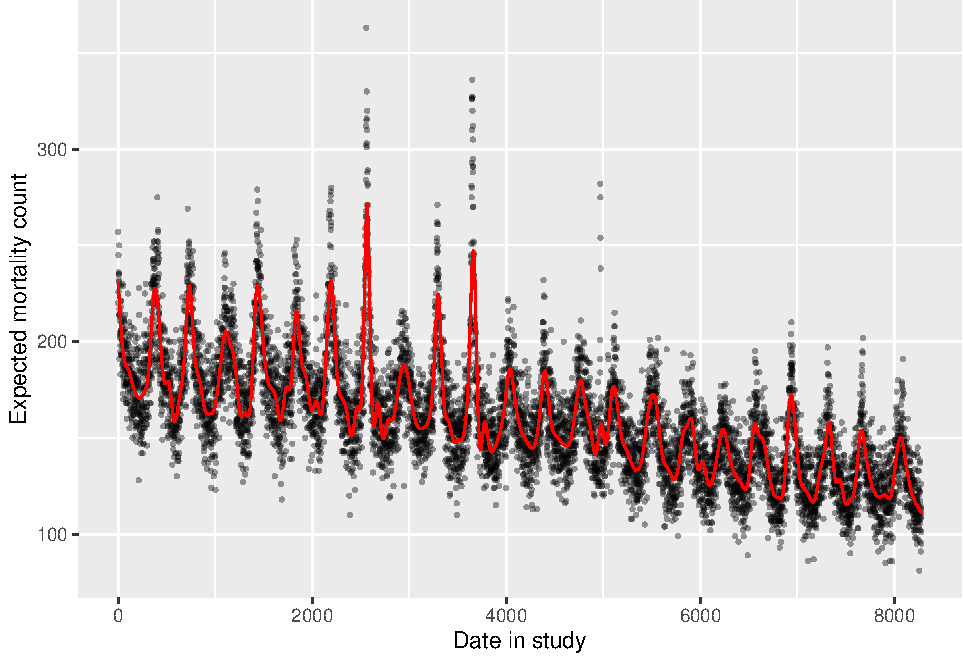
\includegraphics{adv_epi_analysis_files/figure-latex/unnamed-chunk-52-1.pdf}

The non-linear term for time has allowed enough flexibility that the model now
captures both long-term and seasonal trends in the data.

You might wonder how many degrees of freedom you should use for this time spline. In practice,
researchers often using about 6--8 degrees of freedom per year of the study, in
the case of year-round data. You can explore how changing the degrees of freedom
changes the way the model fits to the observed data. As you use more degrees of
freedom, the line will capture very short-term effects, and may start to
interfere with the shorter-term associations between environmental exposures and
health risk that you are trying to capture. Even in the example model we just
fit, for example, it looks like the control for time may be capturing some
patterns that were likely caused by heatwaves (the rare summer peaks, including
one from the 1995 heatwave). Conversely, if too few degrees of freedom are used,
the model will shift to look much more like the linear model, with inadequate
control for seasonal patterns.

\begin{Shaded}
\begin{Highlighting}[]
\CommentTok{\# A model with many less d.f. for the time spline}
\NormalTok{mod\_time\_nonlin\_lowdf }\OtherTok{\textless{}{-}} \FunctionTok{glm}\NormalTok{(all }\SpecialCharTok{\textasciitilde{}} \FunctionTok{ns}\NormalTok{(time, }\AttributeTok{df =} \DecValTok{10}\NormalTok{), }
                             \AttributeTok{data =}\NormalTok{ obs, }\AttributeTok{family =} \StringTok{"quasipoisson"}\NormalTok{)}
\NormalTok{mod\_time\_nonlin\_lowdf }\SpecialCharTok{\%\textgreater{}\%} 
  \FunctionTok{augment}\NormalTok{() }\SpecialCharTok{\%\textgreater{}\%} 
  \FunctionTok{mutate}\NormalTok{(}\AttributeTok{time =}\NormalTok{ obs}\SpecialCharTok{$}\NormalTok{time) }\SpecialCharTok{\%\textgreater{}\%} 
  \FunctionTok{ggplot}\NormalTok{(}\FunctionTok{aes}\NormalTok{(}\AttributeTok{x =}\NormalTok{ time)) }\SpecialCharTok{+} 
  \FunctionTok{geom\_point}\NormalTok{(}\FunctionTok{aes}\NormalTok{(}\AttributeTok{y =}\NormalTok{ all), }\AttributeTok{alpha =} \FloatTok{0.4}\NormalTok{, }\AttributeTok{size =} \FloatTok{0.5}\NormalTok{) }\SpecialCharTok{+} 
  \FunctionTok{geom\_line}\NormalTok{(}\FunctionTok{aes}\NormalTok{(}\AttributeTok{y =} \FunctionTok{exp}\NormalTok{(.fitted)), }\AttributeTok{color =} \StringTok{"red"}\NormalTok{) }\SpecialCharTok{+} 
  \FunctionTok{labs}\NormalTok{(}\AttributeTok{x =} \StringTok{"Date in study"}\NormalTok{, }\AttributeTok{y =} \StringTok{"Expected mortality count"}\NormalTok{) }
\end{Highlighting}
\end{Shaded}

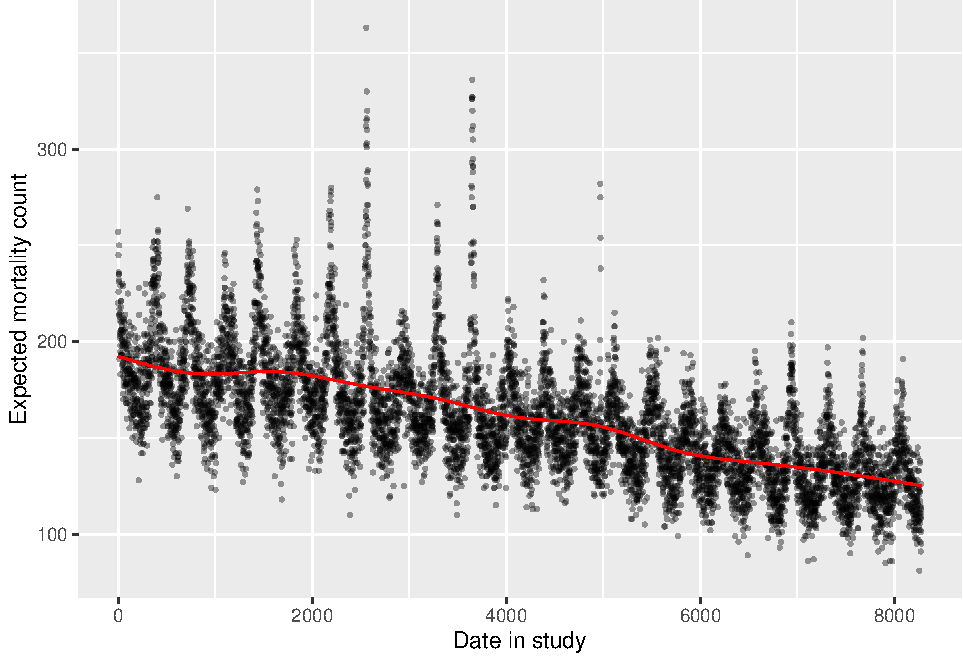
\includegraphics{adv_epi_analysis_files/figure-latex/unnamed-chunk-53-1.pdf}

\begin{Shaded}
\begin{Highlighting}[]
\CommentTok{\# A model with many more d.f. for the time spline}
\CommentTok{\# (Takes a little while to run)}
\NormalTok{mod\_time\_nonlin\_highdf }\OtherTok{\textless{}{-}} \FunctionTok{glm}\NormalTok{(all }\SpecialCharTok{\textasciitilde{}} \FunctionTok{ns}\NormalTok{(time, }\AttributeTok{df =} \DecValTok{400}\NormalTok{), }
                             \AttributeTok{data =}\NormalTok{ obs, }\AttributeTok{family =} \StringTok{"quasipoisson"}\NormalTok{)}
\NormalTok{mod\_time\_nonlin\_highdf }\SpecialCharTok{\%\textgreater{}\%} 
  \FunctionTok{augment}\NormalTok{() }\SpecialCharTok{\%\textgreater{}\%} 
  \FunctionTok{mutate}\NormalTok{(}\AttributeTok{time =}\NormalTok{ obs}\SpecialCharTok{$}\NormalTok{time) }\SpecialCharTok{\%\textgreater{}\%} 
  \FunctionTok{ggplot}\NormalTok{(}\FunctionTok{aes}\NormalTok{(}\AttributeTok{x =}\NormalTok{ time)) }\SpecialCharTok{+} 
  \FunctionTok{geom\_point}\NormalTok{(}\FunctionTok{aes}\NormalTok{(}\AttributeTok{y =}\NormalTok{ all), }\AttributeTok{alpha =} \FloatTok{0.4}\NormalTok{, }\AttributeTok{size =} \FloatTok{0.5}\NormalTok{) }\SpecialCharTok{+} 
  \FunctionTok{geom\_line}\NormalTok{(}\FunctionTok{aes}\NormalTok{(}\AttributeTok{y =} \FunctionTok{exp}\NormalTok{(.fitted)), }\AttributeTok{color =} \StringTok{"red"}\NormalTok{) }\SpecialCharTok{+} 
  \FunctionTok{labs}\NormalTok{(}\AttributeTok{x =} \StringTok{"Date in study"}\NormalTok{, }\AttributeTok{y =} \StringTok{"Expected mortality count"}\NormalTok{) }
\end{Highlighting}
\end{Shaded}

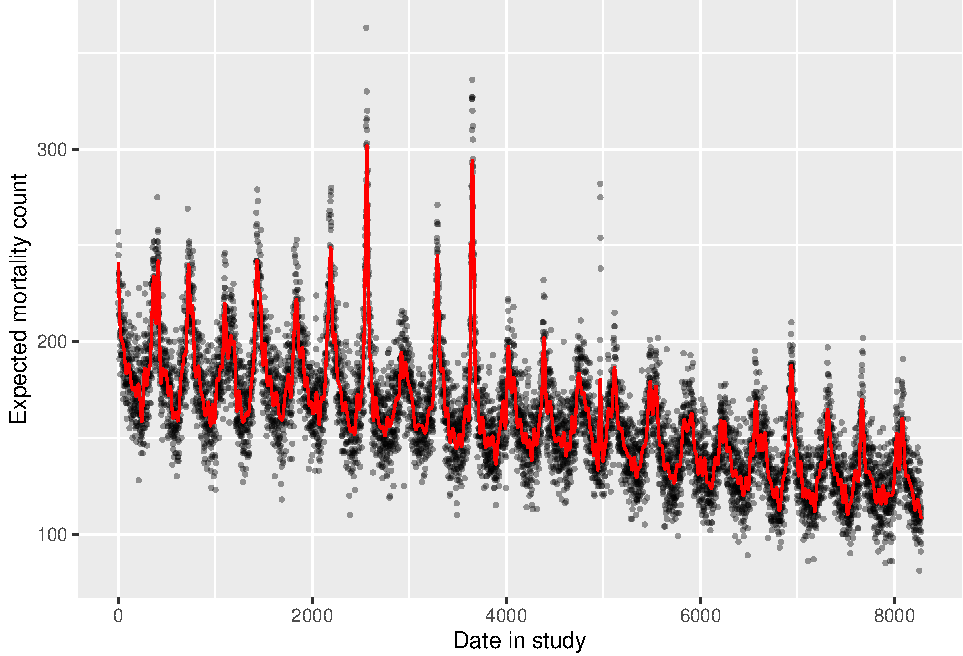
\includegraphics{adv_epi_analysis_files/figure-latex/unnamed-chunk-54-1.pdf}

In all cases, when you fit a non-linear function of an explanatory variable,
it will make the model summary results look much more complicated, e.g.:

\begin{Shaded}
\begin{Highlighting}[]
\NormalTok{mod\_time\_nonlin\_lowdf }\SpecialCharTok{\%\textgreater{}\%} 
  \FunctionTok{tidy}\NormalTok{()}
\end{Highlighting}
\end{Shaded}

\begin{verbatim}
## # A tibble: 11 x 5
##    term                estimate std.error statistic   p.value
##    <chr>                  <dbl>     <dbl>     <dbl>     <dbl>
##  1 (Intercept)           5.26     0.00948    555.   0        
##  2 ns(time, df = 10)1   -0.0260   0.0119      -2.18 2.93e-  2
##  3 ns(time, df = 10)2   -0.0860   0.0155      -5.56 2.85e-  8
##  4 ns(time, df = 10)3   -0.114    0.0139      -8.15 4.01e- 16
##  5 ns(time, df = 10)4   -0.196    0.0151     -13.0  4.47e- 38
##  6 ns(time, df = 10)5   -0.187    0.0148     -12.6  2.80e- 36
##  7 ns(time, df = 10)6   -0.315    0.0154     -20.5  5.62e- 91
##  8 ns(time, df = 10)7   -0.337    0.0154     -21.9  1.95e-103
##  9 ns(time, df = 10)8   -0.358    0.0135     -26.5  1.56e-148
## 10 ns(time, df = 10)9   -0.467    0.0244     -19.2  4.49e- 80
## 11 ns(time, df = 10)10  -0.392    0.0126     -31.2  8.01e-202
\end{verbatim}

You can see that there are multiple model coefficients for the variable fit
using a spline function, the same as the number of degrees of freedom. These
model coefficients are very hard to interpret on their own. When we are using
the spline to \emph{control} for a factor that might serve as a confounder of the
association of interest, we typically won't need to try to interpret these
model coefficients---instead, we are interested in accounting for how this
factor explains variability in the outcome, without needing to quantify the
association as a key result. However, there are also cases where we want to
use a spline to fit the association with the exposure that we are interested
in. In this case, we will want to be able to interpret model coefficients from
the spline. Later in this chapter, we will introduce the \texttt{dlnm} package, which
includes functions to both fit and interpret natural cubic splines within
GLMs for environmental epidemiology.

\begin{enumerate}
\def\labelenumi{\arabic{enumi}.}
\setcounter{enumi}{1}
\tightlist
\item
  \textbf{Start from the last model created in the last chapter and add control for
  long-term and seasonal trends over the study period.}
\end{enumerate}

The last model fit in the last chapter was the following, which fits for the
association between a linear term of temperature and mortality risk, with control
for day of week:

\begin{Shaded}
\begin{Highlighting}[]
\NormalTok{mod\_ctrl\_dow }\OtherTok{\textless{}{-}} \FunctionTok{glm}\NormalTok{(all }\SpecialCharTok{\textasciitilde{}}\NormalTok{ tmean }\SpecialCharTok{+} \FunctionTok{factor}\NormalTok{(dow, }\AttributeTok{ordered =} \ConstantTok{FALSE}\NormalTok{), }
                    \AttributeTok{data =}\NormalTok{ obs, }\AttributeTok{family =} \StringTok{"quasipoisson"}\NormalTok{)}
\end{Highlighting}
\end{Shaded}

To add control for long-term and seasonal trends, you can take the natural cubic
spline function of temperature that you just fit and include it among the
explanatory / independent variables from the model in the last chapter. If you
want to control for only long-term trends, a linear term of the \texttt{time} column
could work, as we discovered in the first part of this chapter's exercise.
However, seasonal trends could certainly confound the association of interest.
Mortality rates have a clear seasonal pattern, and temperature does as well,
and these patterns create the potential for confounding when we look at how
temperature and mortality risk are associated, beyond any seasonally-driven
pathways.

\begin{Shaded}
\begin{Highlighting}[]
\NormalTok{mod\_ctrl\_dow\_time }\OtherTok{\textless{}{-}} \FunctionTok{glm}\NormalTok{(all }\SpecialCharTok{\textasciitilde{}}\NormalTok{ tmean }\SpecialCharTok{+} \FunctionTok{factor}\NormalTok{(dow, }\AttributeTok{ordered =} \ConstantTok{FALSE}\NormalTok{) }\SpecialCharTok{+}
                           \FunctionTok{ns}\NormalTok{(time, }\AttributeTok{df =} \DecValTok{158}\NormalTok{), }
                         \AttributeTok{data =}\NormalTok{ obs, }\AttributeTok{family =} \StringTok{"quasipoisson"}\NormalTok{)}
\end{Highlighting}
\end{Shaded}

You can see the influence of this seasonal confounding if you look at the model
results. When we look at the results from the model that did not control for
long-term and seasonal trends, we get an estimate that mortality rates tend to
be lower on days with higher temperature, with a negative term for \texttt{tmean}:

\begin{Shaded}
\begin{Highlighting}[]
\NormalTok{mod\_ctrl\_dow }\SpecialCharTok{\%\textgreater{}\%} 
  \FunctionTok{tidy}\NormalTok{() }\SpecialCharTok{\%\textgreater{}\%} 
  \FunctionTok{filter}\NormalTok{(term }\SpecialCharTok{==} \StringTok{"tmean"}\NormalTok{)}
\end{Highlighting}
\end{Shaded}

\begin{verbatim}
## # A tibble: 1 x 5
##   term  estimate std.error statistic p.value
##   <chr>    <dbl>     <dbl>     <dbl>   <dbl>
## 1 tmean  -0.0148  0.000354     -41.7       0
\end{verbatim}

Conversely, when we include control for long-term and seasonal trends, the
estimated association between mortality rates and temperature is reversed,
estimating increased mortality rates on days with higher temperature, \emph{controlling
for long-term and seasonal trends}:

\begin{Shaded}
\begin{Highlighting}[]
\NormalTok{mod\_ctrl\_dow\_time }\SpecialCharTok{\%\textgreater{}\%} 
  \FunctionTok{tidy}\NormalTok{() }\SpecialCharTok{\%\textgreater{}\%} 
  \FunctionTok{filter}\NormalTok{(term }\SpecialCharTok{==} \StringTok{"tmean"}\NormalTok{)}
\end{Highlighting}
\end{Shaded}

\begin{verbatim}
## # A tibble: 1 x 5
##   term  estimate std.error statistic  p.value
##   <chr>    <dbl>     <dbl>     <dbl>    <dbl>
## 1 tmean  0.00370  0.000395      9.36 1.02e-20
\end{verbatim}

\begin{enumerate}
\def\labelenumi{\arabic{enumi}.}
\setcounter{enumi}{2}
\tightlist
\item
  \textbf{Refine your model to fit for a non-linear, rather than linear, function
  of temperature in the model.}
\end{enumerate}

You can use a spline in the same way to fit a non-linear function for the
exposure of interest in the model (temperature). We'll start there. However,
as mentioned earlier, it's a bit tricky to interpret the coefficients from the
fit model---you no longer generate a single coefficient for the exposure of
interest, but instead several related to the spline. Therefore, once we show
how to fit using \texttt{ns} directly, we'll show how you can do the same thing using
specialized functions in the \texttt{dlnm} package. This package includes a lot of
nice functions for not only fitting an association using a non-linear term,
but also for interpreting the results after the model is fit.

First, here is code that can be used to fit the model using \texttt{ns} directly,
similarly to the approach we used to control for temporal patterns with a
flexible function:

\begin{Shaded}
\begin{Highlighting}[]
\NormalTok{mod\_ctrl\_nl\_temp }\OtherTok{\textless{}{-}} \FunctionTok{glm}\NormalTok{(all }\SpecialCharTok{\textasciitilde{}} \FunctionTok{ns}\NormalTok{(tmean, }\DecValTok{4}\NormalTok{) }\SpecialCharTok{+} \FunctionTok{factor}\NormalTok{(dow, }\AttributeTok{ordered =} \ConstantTok{FALSE}\NormalTok{) }\SpecialCharTok{+}
                          \FunctionTok{ns}\NormalTok{(time, }\AttributeTok{df =} \DecValTok{158}\NormalTok{), }
                        \AttributeTok{data =}\NormalTok{ obs, }\AttributeTok{family =} \StringTok{"quasipoisson"}\NormalTok{)}
\end{Highlighting}
\end{Shaded}

We can plot the predicted values from this fitted model (red points in the plot below)
compared to the observed data (black dots) using our usual method of using \texttt{augment} to
extract the predicted values:

\begin{Shaded}
\begin{Highlighting}[]
\NormalTok{mod\_ctrl\_nl\_temp }\SpecialCharTok{\%\textgreater{}\%} 
  \FunctionTok{augment}\NormalTok{() }\SpecialCharTok{\%\textgreater{}\%} 
  \FunctionTok{mutate}\NormalTok{(}\AttributeTok{tmean =}\NormalTok{ obs}\SpecialCharTok{$}\NormalTok{tmean) }\SpecialCharTok{\%\textgreater{}\%} 
  \FunctionTok{ggplot}\NormalTok{(}\FunctionTok{aes}\NormalTok{(}\AttributeTok{x =}\NormalTok{ tmean)) }\SpecialCharTok{+} 
  \FunctionTok{geom\_point}\NormalTok{(}\FunctionTok{aes}\NormalTok{(}\AttributeTok{y =}\NormalTok{ all), }\AttributeTok{alpha =} \FloatTok{0.4}\NormalTok{, }\AttributeTok{size =} \FloatTok{0.5}\NormalTok{) }\SpecialCharTok{+} 
  \FunctionTok{geom\_point}\NormalTok{(}\FunctionTok{aes}\NormalTok{(}\AttributeTok{y =} \FunctionTok{exp}\NormalTok{(.fitted)), }\AttributeTok{color =} \StringTok{"red"}\NormalTok{,  }\AttributeTok{size =} \FloatTok{0.4}\NormalTok{) }\SpecialCharTok{+} 
  \FunctionTok{labs}\NormalTok{(}\AttributeTok{x =} \StringTok{"Daily mean temperature"}\NormalTok{, }\AttributeTok{y =} \StringTok{"Expected mortality count"}\NormalTok{) }
\end{Highlighting}
\end{Shaded}

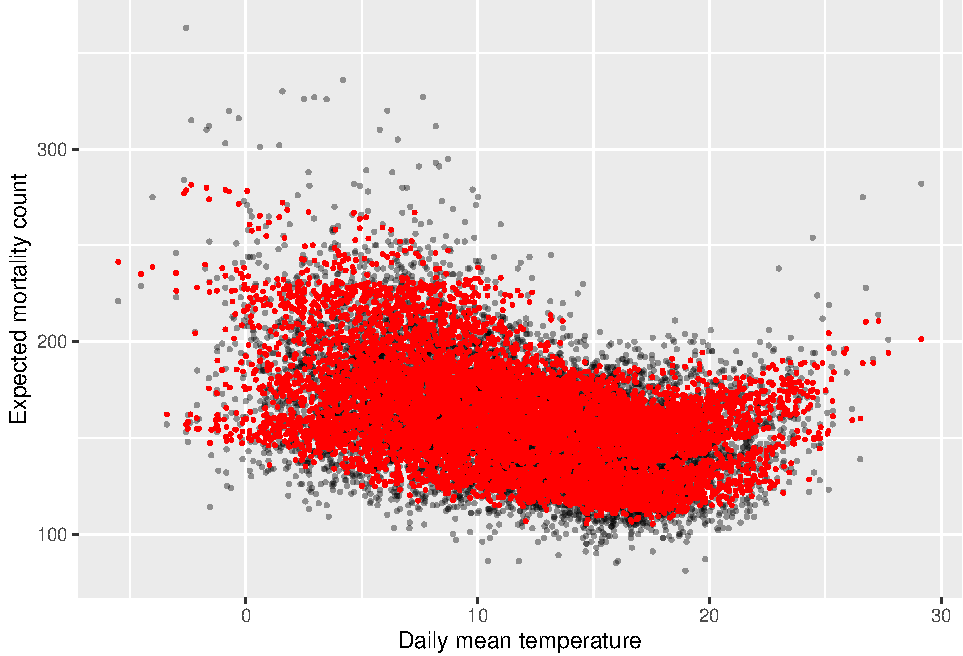
\includegraphics{adv_epi_analysis_files/figure-latex/unnamed-chunk-61-1.pdf}

However, these predictions are very variable at any given temperature. This reflects how
other independent variables, like long-term and seasonal trends, explain variability in
mortality. This makes sense, but it makes it a bit hard to investigate the role of temperature
specifically. Let's look, then, at some other options for viewing the results that will
help us focus on the association of the exposure we care about (temperature) with the outcome.

The next part has a lot of steps, so it might at first seem confusing. However, fortunately
we won't always have to do all the steps ourselves---there is a nice R package that
will help us. We'll look at the process first, though, and then the easier way to use a
package to help with some of the steps. Also, this process gives us a first look at how
the idea of basis functions work. We'll later expand on these to look at non-linear
relationships with the exposure at different lag times, using cross-basis functions, so this
forms a starting point for moving into the idea of a cross-basis.

First, we need to think about how temperature gets included in the regression
model---specifically, as a function of \emph{basis variables} rather than as a single variable.
In other words, to include temperature as a nonlinear function, we're going to create
a structure in the regression equation that includes the variable of temperature in
several different terms, in different transformations in each term. I simple example of this
is a second-degree polynomial. If we wanted to include a second-order polynomial function
of temperature in the regression, then we'd use the following basis:

\[
\beta_1 T + \beta_2 T^2
\]

Notice that here we're using the same independent variable (\(T\), which stands for daily
temperature), but we're including both untransformed \(T\) and also \(T\) squared. This function
of \(T\) might go into the regression equation as something like:

\[
E(Y) = \alpha + \beta_1 T + \beta_2 T^2 + ns(time) + \mathbf{\gamma^{'}D}
\]
where \(\alpha\) is the intercept, \(ns(time)\) is a natural cubic spline that controls for
time (long-term and seasonal trends) and \(\mathbf{D}\) is day of week, with \(\mathbf{\gamma}\) as
the set of coefficients associated with day of week. (Here, I've included the outcome,
\(Y\), untransformed, as you would for a linear regression, but of course the same idea
works with Poisson regression, when you'd instead have \(log(E(Y))\) on the left of the
equation.)

When you fit a regression model in a program like R, it sets up the observed data into
something called a \emph{model matrix}, where it has the values for each observation for each of
the independent variables you want to include, plus a column of ``1''s for the intercept, if you
model structure includes one. The regression model will fit a coefficient
for each of these columns in the model matrix. In a simple case, this model matrix will just
repeat each of your independent variables. For example, the model matrix for the model
\texttt{mod\_overdisp\_reg}, which we fit in the last chapter and which included only an intercept
and a linear term for \texttt{tmean}, looks like this (the \texttt{model.matrix} function will give you
the model matrix of any \texttt{glm} object that you get by running the \texttt{glm} function in R):

\begin{Shaded}
\begin{Highlighting}[]
\NormalTok{mod\_ovdisp\_reg }\SpecialCharTok{\%\textgreater{}\%} 
  \FunctionTok{model.matrix}\NormalTok{() }\SpecialCharTok{\%\textgreater{}\%} 
  \FunctionTok{head}\NormalTok{()}
\end{Highlighting}
\end{Shaded}

\begin{verbatim}
##   (Intercept)    tmean
## 1           1 3.913589
## 2           1 5.547919
## 3           1 4.385564
## 4           1 5.431046
## 5           1 6.867855
## 6           1 9.232628
\end{verbatim}

We already start using the idea of basis variables when we include categorical variables, like
day of week. Here is the model matrix for the \texttt{mod\_ctrl\_dow} model that we fit in the last
chapter:

\begin{Shaded}
\begin{Highlighting}[]
\NormalTok{mod\_ctrl\_dow }\SpecialCharTok{\%\textgreater{}\%} 
  \FunctionTok{model.matrix}\NormalTok{() }\SpecialCharTok{\%\textgreater{}\%} 
  \FunctionTok{head}\NormalTok{()}
\end{Highlighting}
\end{Shaded}

\begin{verbatim}
##   (Intercept)    tmean factor(dow, ordered = FALSE)Mon
## 1           1 3.913589                               1
## 2           1 5.547919                               0
## 3           1 4.385564                               0
## 4           1 5.431046                               0
## 5           1 6.867855                               0
## 6           1 9.232628                               0
##   factor(dow, ordered = FALSE)Tue factor(dow, ordered = FALSE)Wed
## 1                               0                               0
## 2                               1                               0
## 3                               0                               1
## 4                               0                               0
## 5                               0                               0
## 6                               0                               0
##   factor(dow, ordered = FALSE)Thu factor(dow, ordered = FALSE)Fri
## 1                               0                               0
## 2                               0                               0
## 3                               0                               0
## 4                               1                               0
## 5                               0                               1
## 6                               0                               0
##   factor(dow, ordered = FALSE)Sat
## 1                               0
## 2                               0
## 3                               0
## 4                               0
## 5                               0
## 6                               1
\end{verbatim}

You can see that the regression call broke the day-of-week variable up into a set of indicator variables, which
equal either 1 or 0. There will be one less of these than the number of categories for the
variable; in otherwords, if the categorical variable took two values (Weekend / Weekday), then
this would be covered by a single column; since there are seven days in the week, the
day-of-week variable breaks into six (7 - 1) columns. The first level of the categories
(Sunday in this case) serves as a baseline and doesn't get a value. The others levels
(Monday, Tuesday, etc.) each get their own indicator variable---so, their own column in
the model matrix---which equals ``1'' on that day (i.e., ``1'' for the Monday column if the date
of the observation is a Monday) and ``0'' on all other days.

Now let's go back and look at the example of including temperature in the model as a nonlinear
function, starting with the simple example of using a second-degree polynomial. What would
the basis for that look like? We can find out by fitting the model and then looking at the
model matrix (the \texttt{I()} function lets us specify a transformation of a column from the
data when we set up the regression equation structure in \texttt{glm}):

\begin{Shaded}
\begin{Highlighting}[]
\NormalTok{mod\_polynomial\_temp }\OtherTok{\textless{}{-}} \FunctionTok{glm}\NormalTok{(all }\SpecialCharTok{\textasciitilde{}}\NormalTok{ tmean }\SpecialCharTok{+} \FunctionTok{I}\NormalTok{(tmean }\SpecialCharTok{\^{}} \DecValTok{2}\NormalTok{), }
                           \AttributeTok{data =}\NormalTok{ obs, }\AttributeTok{family =} \StringTok{"quasipoisson"}\NormalTok{)}
\NormalTok{mod\_polynomial\_temp }\SpecialCharTok{\%\textgreater{}\%} 
  \FunctionTok{model.matrix}\NormalTok{() }\SpecialCharTok{\%\textgreater{}\%} 
  \FunctionTok{head}\NormalTok{()}
\end{Highlighting}
\end{Shaded}

\begin{verbatim}
##   (Intercept)    tmean I(tmean^2)
## 1           1 3.913589   15.31618
## 2           1 5.547919   30.77941
## 3           1 4.385564   19.23317
## 4           1 5.431046   29.49627
## 5           1 6.867855   47.16743
## 6           1 9.232628   85.24142
\end{verbatim}

You can see that this has created two columns based on the temperature variable, one with
it untransformed and one with it squared. The regression will estimate coefficients for each
of these basis variables of temperature, and then that allows you to fit a model with a
function of temperature, rather than solely temperature. Here are the coefficients from
this model:

\begin{Shaded}
\begin{Highlighting}[]
\NormalTok{mod\_polynomial\_temp }\SpecialCharTok{\%\textgreater{}\%} 
  \FunctionTok{tidy}\NormalTok{()}
\end{Highlighting}
\end{Shaded}

\begin{verbatim}
## # A tibble: 3 x 5
##   term         estimate std.error statistic   p.value
##   <chr>           <dbl>     <dbl>     <dbl>     <dbl>
## 1 (Intercept)  5.31     0.00675       787.  0        
## 2 tmean       -0.0298   0.00126       -23.6 2.27e-119
## 3 I(tmean^2)   0.000667 0.0000538      12.4 5.70e- 35
\end{verbatim}

Therefore, it's fit the following model to describe the association between temperature and
mortality:

\[
log(E(Y)) = 5.3092 - 0.0298T + 0.0007T^2
\]
If you want to estimate the relative risk of mortality at 15 degrees Celsius versus 10
degrees Celsius with this model (which is confounded by long-term and seasonal trends, so
has some issues we'll want to fix), you can take the following process. Take the two
equations for the expected mortality when \(T\) is 15 and 10, respectively:

\[
log(E(Y|T=15)) = 5.3092 - 0.0298(15) + 0.0007(15^2) \\
log(E(Y|T=10)) = 5.3092 - 0.0298(10) + 0.0007(10^2)  
\]
If you subtract the second from the first, you get:

\[
log(E(Y|T=15)) - log(E(Y|T=10)) = (5.3092 - 5.3092) - 0.0298(15 - 10) + 0.0007(15^2 - 10^2)
\]
which simplifies to (if the left part isn't clear, review the rules for how you can manipulate logarithms):

\[
log(\frac{E(Y|T=15)}{E(Y|T=10)}) = - 0.0298(5) + 0.0007(125) = -0.0615
\]
Exponentiate both sides, to get to the relative risk at 15 degrees versus 10 degrees (in
other words, the ratio of expected mortality at 15 degrees to that at 10 degrees):

\[
\frac{E(Y|T=15)}{E(Y|T=10)} = e^{-0.0615} =  0.94
\]
You can see that the basis variables are great in helping us explore how an independent
variable might be related to the outcome in a non-linear way, but there's a bit of a cost
in terms of us needing to take some extra steps to interpret the results from that model.
Also, note that there's not a single coefficient that we can extract from the model as
a summary of the relationship. Instead, we needed to pick a reference temperature (10 degrees
in this example) and compare to that to get an estimated relative risk. We'll see the
same pattern as we move to using natural cubic splines to create the basis variables for
temperature.

Now let's move to a spline. The function the spline runs to transform the temperature
variable into the different basis variables is more complex than for the polynomial example,
but the result is similar: you get several columns to fit in the model for a variable, compared
to the single column you would include if you were only fitting a linear term. If you
take a look at the output of running the \texttt{ns} function on temperature in the data, you can
see that it creates several new columns (one for each degree of freedom), which will be the
basis variables in the regression:

\begin{Shaded}
\begin{Highlighting}[]
\FunctionTok{ns}\NormalTok{(obs}\SpecialCharTok{$}\NormalTok{tmean, }\AttributeTok{df =} \DecValTok{4}\NormalTok{) }\SpecialCharTok{\%\textgreater{}\%} 
  \FunctionTok{head}\NormalTok{()}
\end{Highlighting}
\end{Shaded}

\begin{verbatim}
##              1           2         3          4
## [1,] 0.1769619 -0.20432696 0.4777110 -0.2733841
## [2,] 0.2860253 -0.19686120 0.4602563 -0.2633951
## [3,] 0.2049283 -0.20410506 0.4771922 -0.2730872
## [4,] 0.2770456 -0.19804188 0.4630167 -0.2649748
## [5,] 0.4012496 -0.17595974 0.4113892 -0.2354295
## [6,] 0.6581858 -0.09844302 0.2476396 -0.1417190
\end{verbatim}

The output from \texttt{ns} also has some metadata, included in the attributes of the object, that
have some other information about the spline function, including where the knots were
placed and where the boundary knots (which are at the outer ranges of the data) are placed.
You can the \texttt{str} function to explore both the data and metadata stored in this object:

\begin{Shaded}
\begin{Highlighting}[]
\FunctionTok{ns}\NormalTok{(obs}\SpecialCharTok{$}\NormalTok{tmean, }\AttributeTok{df =} \DecValTok{4}\NormalTok{) }\SpecialCharTok{\%\textgreater{}\%} 
  \FunctionTok{str}\NormalTok{()}
\end{Highlighting}
\end{Shaded}

\begin{verbatim}
##  'ns' num [1:8279, 1:4] 0.177 0.286 0.205 0.277 0.401 ...
##  - attr(*, "dimnames")=List of 2
##   ..$ : NULL
##   ..$ : chr [1:4] "1" "2" "3" "4"
##  - attr(*, "degree")= int 3
##  - attr(*, "knots")= num [1:3] 7.47 11.47 15.93
##  - attr(*, "Boundary.knots")= num [1:2] -5.5 29.1
##  - attr(*, "intercept")= logi FALSE
\end{verbatim}

This is saying, for example, that the internal knots for this spline were put at the
25th, 50th, and 75th quantiles of the temperature data, where were 7.47 degrees, 11.47 degrees,
and 15.93 degrees. (The defaults for \texttt{ns} is to place knots evenly at percentiles, based
on the number of degrees of freedom you specify. You can change this by placing the knots
``by hand'', using the \texttt{knots} argument in the \texttt{ns} function.)

This spline object can be used not just for its basis values, but also to ``predict'' new
basis values for a new set of temperature values. For example, you could figure out
what the basis values from this spline would be for every degree of temperature between
-6 and 29 using the following code:

\begin{Shaded}
\begin{Highlighting}[]
\NormalTok{temp\_spline }\OtherTok{\textless{}{-}} \FunctionTok{ns}\NormalTok{(obs}\SpecialCharTok{$}\NormalTok{tmean, }\AttributeTok{df =} \DecValTok{4}\NormalTok{)}
\NormalTok{temp\_spline\_preds }\OtherTok{\textless{}{-}} \FunctionTok{predict}\NormalTok{(temp\_spline, }\AttributeTok{newx =} \SpecialCharTok{{-}}\DecValTok{5}\SpecialCharTok{:}\DecValTok{30}\NormalTok{)}
\NormalTok{temp\_spline\_preds }\SpecialCharTok{\%\textgreater{}\%} 
  \FunctionTok{head}\NormalTok{()}
\end{Highlighting}
\end{Shaded}

\begin{verbatim}
##                 1           2          3           4
## [1,] 2.689545e-05 -0.01606406 0.03755734 -0.02149328
## [2,] 7.189726e-04 -0.04768237 0.11148013 -0.06379775
## [3,] 3.321933e-03 -0.07825364 0.18295494 -0.10470130
## [4,] 9.107577e-03 -0.10708098 0.25035250 -0.14327152
## [5,] 1.934771e-02 -0.13346753 0.31204355 -0.17857602
## [6,] 3.531412e-02 -0.15671641 0.36639881 -0.20968240
\end{verbatim}

This is handy, because it will help us visualize the relationship we fit in a regression
model---we can start with these basis values for each degree in our temperature range, and
then use the regression coefficients for each basis variable to estimate relative risk
at that temperature compared to a reference temperature, exactly as we did in the equations
for the polynomial function of temperature earlier, comparing 15 degrees C to the reference
of 10 degrees.

All we need now are the regression coefficients for each of these temperature basis
variables. We can extract those from the model we fit earlier, where we included
\texttt{ns(tmean,\ 4)} as one of the model terms. Here, I'm using \texttt{tidy} to get the model
coefficients and then, because there are \emph{lots} of them (from fitting a spline for
time with lots of degrees of freedom), I'm using the \texttt{str\_detect} function from the
\texttt{stringr} package to pick out just those with ``tmean'' in the \texttt{term} column:

\begin{Shaded}
\begin{Highlighting}[]
\NormalTok{mod\_ctrl\_nl\_temp }\SpecialCharTok{\%\textgreater{}\%} 
  \FunctionTok{tidy}\NormalTok{() }\SpecialCharTok{\%\textgreater{}\%} 
  \FunctionTok{filter}\NormalTok{(}\FunctionTok{str\_detect}\NormalTok{(term, }\StringTok{"tmean"}\NormalTok{))}
\end{Highlighting}
\end{Shaded}

\begin{verbatim}
## # A tibble: 4 x 5
##   term          estimate std.error statistic  p.value
##   <chr>            <dbl>     <dbl>     <dbl>    <dbl>
## 1 ns(tmean, 4)1  -0.0700    0.0135    -5.18  2.30e- 7
## 2 ns(tmean, 4)2  -0.0660    0.0126    -5.24  1.61e- 7
## 3 ns(tmean, 4)3   0.0110    0.0313     0.350 7.26e- 1
## 4 ns(tmean, 4)4   0.347     0.0177    19.6   2.02e-83
\end{verbatim}

You can add on \texttt{pull} to pull out just the \texttt{estimate} column as a vector, which will be
helpful when we want to multiple these coefficients by the basis values for each degree
of temperature across our temperature range:

\begin{Shaded}
\begin{Highlighting}[]
\NormalTok{temp\_spline\_ests }\OtherTok{\textless{}{-}}\NormalTok{ mod\_ctrl\_nl\_temp }\SpecialCharTok{\%\textgreater{}\%} 
  \FunctionTok{tidy}\NormalTok{() }\SpecialCharTok{\%\textgreater{}\%} 
  \FunctionTok{filter}\NormalTok{(}\FunctionTok{str\_detect}\NormalTok{(term, }\StringTok{"tmean"}\NormalTok{)) }\SpecialCharTok{\%\textgreater{}\%} 
  \FunctionTok{pull}\NormalTok{(estimate)}
\NormalTok{temp\_spline\_ests}
\end{Highlighting}
\end{Shaded}

\begin{verbatim}
## [1] -0.06995454 -0.06596939  0.01095574  0.34659715
\end{verbatim}

Now, let's put this together to see how relative risk of mortality changes as you move
across the temperature range! First, we can set up a dataframe that has a column with
each unit of temperature across our range---these are the temperatures where we want to
estimate relative risk---and then the estimated relative risk at that temperature. By
default, we'll be comparing to the lowest temperature in the original data, but we'll talk
in a minute about how to adjust to a different reference temperature. You can use
matrix multiplication (\texttt{\%*\%}) as a shorthand way to multiple each column of the spline
basis variables from \texttt{temp\_spline\_preds} by its estimated coefficient from the regression
model, saved in \texttt{temp\_spline\_ests}, and then add all of those values together (this is
the same idea as what we did in the equations earlier, for the polynomial basis). Then,
to get from log relative risk to relative risk, we'll exponentiate that with \texttt{exp}. You
can see the first rows of the results below:

\begin{Shaded}
\begin{Highlighting}[]
\NormalTok{pred\_temp\_function }\OtherTok{\textless{}{-}} \FunctionTok{tibble}\NormalTok{(}
  \AttributeTok{temp =} \SpecialCharTok{{-}}\DecValTok{5}\SpecialCharTok{:}\DecValTok{30}\NormalTok{, }
  \AttributeTok{temp\_func =}\NormalTok{ temp\_spline\_preds }\SpecialCharTok{\%*\%}\NormalTok{ temp\_spline\_ests,}
  \AttributeTok{rr =} \FunctionTok{exp}\NormalTok{(temp\_func)}
\NormalTok{)}

\NormalTok{pred\_temp\_function }\SpecialCharTok{\%\textgreater{}\%} 
  \FunctionTok{head}\NormalTok{()}
\end{Highlighting}
\end{Shaded}

\begin{verbatim}
## # A tibble: 6 x 3
##    temp temp_func[,1] rr[,1]
##   <int>         <dbl>  <dbl>
## 1    -5      -0.00598  0.994
## 2    -4      -0.0178   0.982
## 3    -3      -0.0294   0.971
## 4    -2      -0.0405   0.960
## 5    -1      -0.0510   0.950
## 6     0      -0.0608   0.941
\end{verbatim}

This is now very easy to plot, with a reference line added at a relative risk of 1.0:

\begin{Shaded}
\begin{Highlighting}[]
\FunctionTok{ggplot}\NormalTok{(pred\_temp\_function, }\FunctionTok{aes}\NormalTok{(}\AttributeTok{x =}\NormalTok{ temp, }\AttributeTok{y =}\NormalTok{ rr)) }\SpecialCharTok{+} 
  \FunctionTok{geom\_point}\NormalTok{() }\SpecialCharTok{+} 
  \FunctionTok{geom\_line}\NormalTok{() }\SpecialCharTok{+} 
  \FunctionTok{labs}\NormalTok{(}\AttributeTok{x =} \StringTok{"Temperature"}\NormalTok{, }
       \AttributeTok{y =} \StringTok{"Relative Risk"}\NormalTok{) }\SpecialCharTok{+} 
  \FunctionTok{geom\_hline}\NormalTok{(}\AttributeTok{yintercept =} \FloatTok{1.0}\NormalTok{, }\AttributeTok{color =} \StringTok{"red"}\NormalTok{, }\AttributeTok{linetype =} \DecValTok{2}\NormalTok{)}
\end{Highlighting}
\end{Shaded}

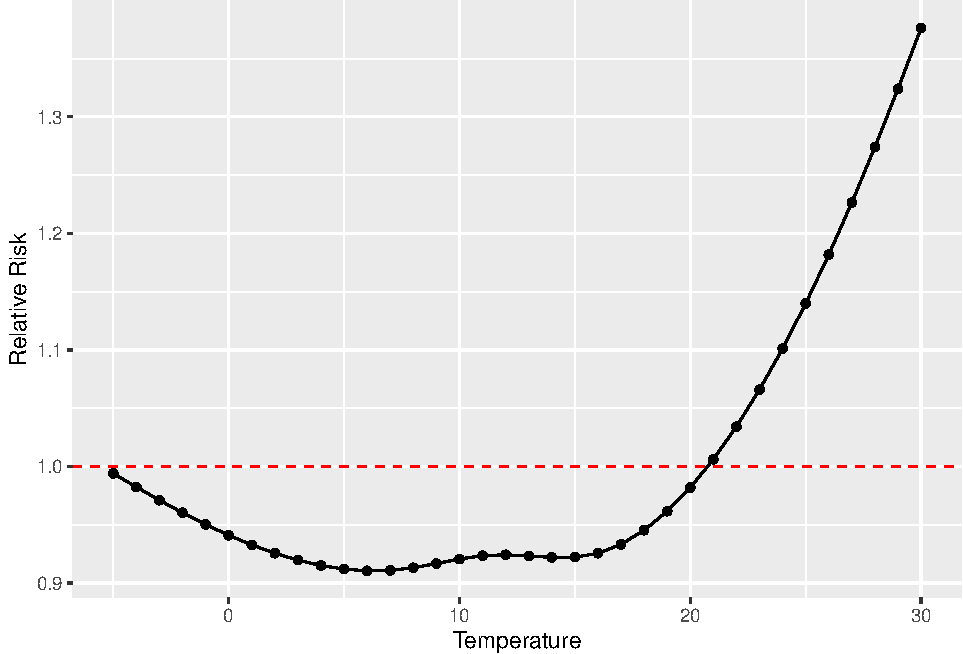
\includegraphics{adv_epi_analysis_files/figure-latex/unnamed-chunk-73-1.pdf}

We might want to shift this, so we're comparing the temperature at which mortality risk
is lowest (sometimes called the \emph{minimum mortality temperature}). This tends to be at
milder temperatures, in the middle of our range, rather than at the minimum temperature in
the range. To start, let's see what temperature aligns with the lowest relative risk of
mortality:

\begin{Shaded}
\begin{Highlighting}[]
\NormalTok{pred\_temp\_function }\SpecialCharTok{\%\textgreater{}\%} 
  \FunctionTok{filter}\NormalTok{(rr }\SpecialCharTok{==} \FunctionTok{min}\NormalTok{(rr))}
\end{Highlighting}
\end{Shaded}

\begin{verbatim}
## Warning: Using one column matrices in `filter()` was deprecated in dplyr 1.1.0.
## i Please use one dimensional logical vectors instead.
## This warning is displayed once every 8 hours.
## Call `lifecycle::last_lifecycle_warnings()` to see where this warning was
## generated.
\end{verbatim}

\begin{verbatim}
## # A tibble: 1 x 3
##    temp temp_func[,1] rr[,1]
##   <int>         <dbl>  <dbl>
## 1     6       -0.0938  0.911
\end{verbatim}

We can therefore realign so that the relative risk equals 1.0 when the temperature is 7 degrees
C, and all other relative risks are relative to a reference temperature of 7 degrees C:

\begin{Shaded}
\begin{Highlighting}[]
\NormalTok{pred\_temp\_function }\OtherTok{\textless{}{-}}\NormalTok{ pred\_temp\_function }\SpecialCharTok{\%\textgreater{}\%} 
  \FunctionTok{mutate}\NormalTok{(}\AttributeTok{temp\_func\_reset =}\NormalTok{ temp\_func }\SpecialCharTok{{-}}\NormalTok{ temp\_func[temp }\SpecialCharTok{==} \DecValTok{7}\NormalTok{],}
         \AttributeTok{rr\_reset =} \FunctionTok{exp}\NormalTok{(temp\_func\_reset)}
\NormalTok{)}

\FunctionTok{ggplot}\NormalTok{(pred\_temp\_function, }\FunctionTok{aes}\NormalTok{(}\AttributeTok{x =}\NormalTok{ temp, }\AttributeTok{y =}\NormalTok{ rr\_reset)) }\SpecialCharTok{+} 
  \FunctionTok{geom\_point}\NormalTok{() }\SpecialCharTok{+} 
  \FunctionTok{geom\_line}\NormalTok{() }\SpecialCharTok{+} 
  \FunctionTok{labs}\NormalTok{(}\AttributeTok{x =} \StringTok{"Temperature"}\NormalTok{, }
       \AttributeTok{y =} \StringTok{"Relative Risk"}\NormalTok{) }\SpecialCharTok{+} 
  \FunctionTok{geom\_hline}\NormalTok{(}\AttributeTok{yintercept =} \FloatTok{1.0}\NormalTok{, }\AttributeTok{color =} \StringTok{"red"}\NormalTok{, }\AttributeTok{linetype =} \DecValTok{2}\NormalTok{)}
\end{Highlighting}
\end{Shaded}

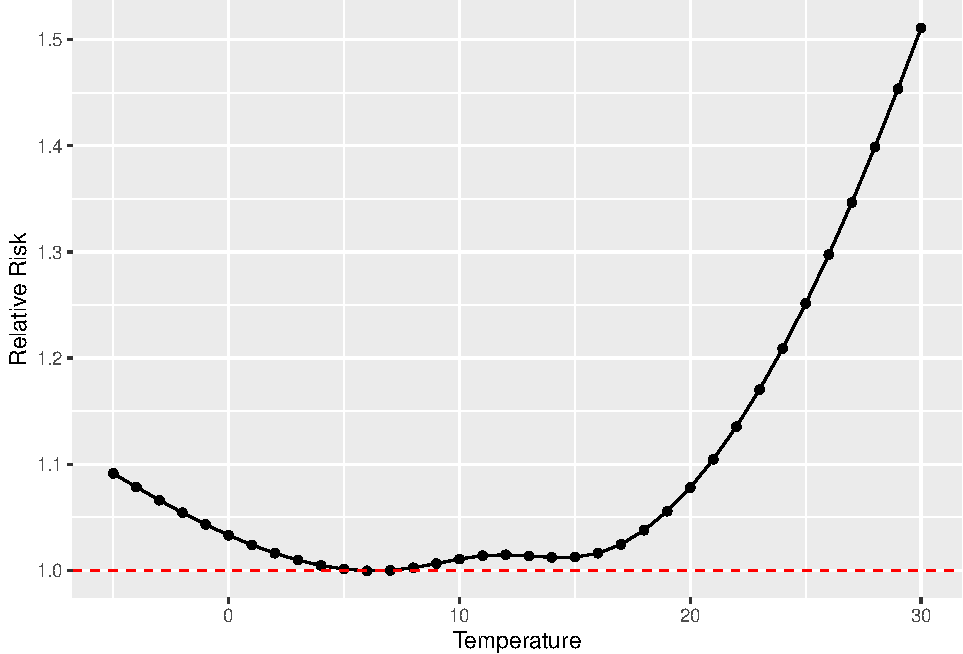
\includegraphics{adv_epi_analysis_files/figure-latex/unnamed-chunk-75-1.pdf}

This is a fairly cumbersome process, as you've seen with this example, and it would be a
pain if we had to do it every time we wanted to visualize and explore results from fitting
regressions that include basis variables from splines. Fortunately, there's a nice R package
called \texttt{dlnm} (for ``distributed lag nonlinear models'') that will help take care of a lot of
these ``under the hood'' steps for us. Even better, this package will let us move on to more
complex crossbasis functions, where we fit non-linear functions in two dimensions, and help
us visualize and interpret results from those models.

To start, make sure you have the \texttt{dlnm} package installed on your computer, and then load
it in your R session. This package has a function called \texttt{crossbasis} that lets you build
a crossbasis function to use in a regression model. We'll talk more about these types
of functions later in this chapter; for right now, we'll be a bit simpler and just use it
to create our spline function of temperature.

In the \texttt{crossbasis} function, you start by putting in the vector of the variable that you
want to expand into basis variables. In our case, this is temperature, which we have saved
as the \texttt{tmean} column in the \texttt{obs} dataset. You use the \texttt{argvar} to give some information
about the basis you want to use for that variable. This will both include the type of
basis function (\texttt{"ns"} for a natural cubic spline), and then also arguments you want to
pass to that basis function, like degrees of freedom (\texttt{df}) or knot locations (\texttt{knots})
if you're fitting a spline. The other arguments allow you to specify a function of lagged
time; we won't use that yet, so you can just include \texttt{lag\ =\ 0} and \texttt{arglag\ =\ list(fun\ =\ "integer")} to create a crossbasis where we only consider same-day effects in a simple way.
If you look at the output, you'll see it's very similar to the basis created by the
\texttt{ns} call earlier (in fact, the values in each column should be identical):

\begin{Shaded}
\begin{Highlighting}[]
\FunctionTok{library}\NormalTok{(dlnm)}
\NormalTok{temp\_basis }\OtherTok{\textless{}{-}} \FunctionTok{crossbasis}\NormalTok{(obs}\SpecialCharTok{$}\NormalTok{tmean, }\AttributeTok{lag =} \DecValTok{0}\NormalTok{, }
                         \AttributeTok{argvar =} \FunctionTok{list}\NormalTok{(}\AttributeTok{fun =} \StringTok{"ns"}\NormalTok{, }\AttributeTok{df =} \DecValTok{4}\NormalTok{), }
                         \AttributeTok{arglag =} \FunctionTok{list}\NormalTok{(}\AttributeTok{fun =} \StringTok{"integer"}\NormalTok{))}
\NormalTok{temp\_basis }\SpecialCharTok{\%\textgreater{}\%} 
  \FunctionTok{head}\NormalTok{()}
\end{Highlighting}
\end{Shaded}

\begin{verbatim}
##          v1.l1       v2.l1     v3.l1      v4.l1
## [1,] 0.1769619 -0.20432696 0.4777110 -0.2733841
## [2,] 0.2860253 -0.19686120 0.4602563 -0.2633951
## [3,] 0.2049283 -0.20410506 0.4771922 -0.2730872
## [4,] 0.2770456 -0.19804188 0.4630167 -0.2649748
## [5,] 0.4012496 -0.17595974 0.4113892 -0.2354295
## [6,] 0.6581858 -0.09844302 0.2476396 -0.1417190
\end{verbatim}

To estimate the regression coefficients, we'll put this whole crossbasis in as one of
our terms in the \texttt{glm} regression equation:

\begin{Shaded}
\begin{Highlighting}[]
\NormalTok{dlnm\_mod\_1 }\OtherTok{\textless{}{-}} \FunctionTok{glm}\NormalTok{(all }\SpecialCharTok{\textasciitilde{}}\NormalTok{ temp\_basis }\SpecialCharTok{+} \FunctionTok{factor}\NormalTok{(dow, }\AttributeTok{ordered =} \ConstantTok{FALSE}\NormalTok{) }\SpecialCharTok{+}
                          \FunctionTok{ns}\NormalTok{(time, }\AttributeTok{df =} \DecValTok{158}\NormalTok{), }
                        \AttributeTok{data =}\NormalTok{ obs, }\AttributeTok{family =} \StringTok{"quasipoisson"}\NormalTok{)}
\end{Highlighting}
\end{Shaded}

As when we fit the spline earlier, you can see that this gives us a set of coefficients,
one for each column in the matrix of crossbasis variables:

\begin{Shaded}
\begin{Highlighting}[]
\NormalTok{dlnm\_mod\_1 }\SpecialCharTok{\%\textgreater{}\%} 
  \FunctionTok{tidy}\NormalTok{() }\SpecialCharTok{\%\textgreater{}\%} 
  \FunctionTok{filter}\NormalTok{(}\FunctionTok{str\_detect}\NormalTok{(term, }\StringTok{"temp\_basis"}\NormalTok{))}
\end{Highlighting}
\end{Shaded}

\begin{verbatim}
## # A tibble: 4 x 5
##   term            estimate std.error statistic  p.value
##   <chr>              <dbl>     <dbl>     <dbl>    <dbl>
## 1 temp_basisv1.l1  -0.0700    0.0135    -5.18  2.30e- 7
## 2 temp_basisv2.l1  -0.0660    0.0126    -5.24  1.61e- 7
## 3 temp_basisv3.l1   0.0110    0.0313     0.350 7.26e- 1
## 4 temp_basisv4.l1   0.347     0.0177    19.6   2.02e-83
\end{verbatim}

However, there's an advantage with using \texttt{crossbasis}, even though it's looked pretty similar
to using \texttt{ns} up to now. That's that there are some special functions that let us predict
and visualize the model results without having to do all the work we did before.

For example, there's a function called \texttt{crosspred} that will give us a number of values,
including the estimated relative risk compared to a reference value. To use this, we
need to input the object name of our crossbasis object (\texttt{temp\_basis}) and the name of our
regression model object (\texttt{dlnm\_mod\_1}). We also want to tell it which temperature we want
to use as our reference (\texttt{cen\ =\ 7} to compare everything to 7 degrees C) and what interval
we want for predictions (\texttt{by\ =\ 1} will give us an estimate for every degree temperature
along our range). The output is a list with a lot of elements, which you can get a view of
with \texttt{str}:

\begin{Shaded}
\begin{Highlighting}[]
\FunctionTok{crosspred}\NormalTok{(}\AttributeTok{basis =}\NormalTok{ temp\_basis, }\AttributeTok{model =}\NormalTok{ dlnm\_mod\_1, }\AttributeTok{cen =} \DecValTok{7}\NormalTok{, }\AttributeTok{by =} \DecValTok{1}\NormalTok{) }\SpecialCharTok{\%\textgreater{}\%} 
  \FunctionTok{str}\NormalTok{()}
\end{Highlighting}
\end{Shaded}

\begin{verbatim}
## List of 19
##  $ predvar     : num [1:35] -5 -4 -3 -2 -1 0 1 2 3 4 ...
##  $ cen         : num 7
##  $ lag         : num [1:2] 0 0
##  $ bylag       : num 1
##  $ coefficients: Named num [1:4] -0.07 -0.066 0.011 0.347
##   ..- attr(*, "names")= chr [1:4] "temp_basisv1.l1" "temp_basisv2.l1" "temp_basisv3.l1" "temp_basisv4.l1"
##  $ vcov        : num [1:4, 1:4] 1.83e-04 1.12e-04 3.85e-04 6.58e-05 1.12e-04 ...
##   ..- attr(*, "dimnames")=List of 2
##   .. ..$ : chr [1:4] "temp_basisv1.l1" "temp_basisv2.l1" "temp_basisv3.l1" "temp_basisv4.l1"
##   .. ..$ : chr [1:4] "temp_basisv1.l1" "temp_basisv2.l1" "temp_basisv3.l1" "temp_basisv4.l1"
##  $ matfit      : num [1:35, 1] 0.0874 0.0756 0.064 0.0529 0.0424 ...
##   ..- attr(*, "dimnames")=List of 2
##   .. ..$ : chr [1:35] "-5" "-4" "-3" "-2" ...
##   .. ..$ : chr [1, 1] "lag0"
##  $ matse       : num [1:35, 1] 0.01435 0.01254 0.01077 0.00907 0.00746 ...
##   ..- attr(*, "dimnames")=List of 2
##   .. ..$ : chr [1:35] "-5" "-4" "-3" "-2" ...
##   .. ..$ : chr [1, 1] "lag0"
##  $ allfit      : Named num [1:35] 0.0874 0.0756 0.064 0.0529 0.0424 ...
##   ..- attr(*, "names")= chr [1:35] "-5" "-4" "-3" "-2" ...
##  $ allse       : Named num [1:35] 0.01435 0.01254 0.01077 0.00907 0.00746 ...
##   ..- attr(*, "names")= chr [1:35] "-5" "-4" "-3" "-2" ...
##  $ matRRfit    : num [1:35, 1] 1.09 1.08 1.07 1.05 1.04 ...
##   ..- attr(*, "dimnames")=List of 2
##   .. ..$ : chr [1:35] "-5" "-4" "-3" "-2" ...
##   .. ..$ : chr [1, 1] "lag0"
##  $ matRRlow    : num [1:35, 1] 1.06 1.05 1.04 1.04 1.03 ...
##   ..- attr(*, "dimnames")=List of 2
##   .. ..$ : chr [1:35] "-5" "-4" "-3" "-2" ...
##   .. ..$ : chr [1, 1] "lag0"
##  $ matRRhigh   : num [1:35, 1] 1.12 1.11 1.09 1.07 1.06 ...
##   ..- attr(*, "dimnames")=List of 2
##   .. ..$ : chr [1:35] "-5" "-4" "-3" "-2" ...
##   .. ..$ : chr [1, 1] "lag0"
##  $ allRRfit    : Named num [1:35] 1.09 1.08 1.07 1.05 1.04 ...
##   ..- attr(*, "names")= chr [1:35] "-5" "-4" "-3" "-2" ...
##  $ allRRlow    : Named num [1:35] 1.06 1.05 1.04 1.04 1.03 ...
##   ..- attr(*, "names")= chr [1:35] "-5" "-4" "-3" "-2" ...
##  $ allRRhigh   : Named num [1:35] 1.12 1.11 1.09 1.07 1.06 ...
##   ..- attr(*, "names")= chr [1:35] "-5" "-4" "-3" "-2" ...
##  $ ci.level    : num 0.95
##  $ model.class : chr [1:2] "glm" "lm"
##  $ model.link  : chr "log"
##  - attr(*, "class")= chr "crosspred"
\end{verbatim}

The one we'll look at right now is \texttt{allRRfit}. You can extract it with (here I'm showing
how you can do it with piping and the \texttt{pluck} function to pull out an element of a list,
but you could do other approaches, too):

\begin{Shaded}
\begin{Highlighting}[]
\NormalTok{est\_rr }\OtherTok{\textless{}{-}}\NormalTok{ dlnm\_mod\_1 }\SpecialCharTok{\%\textgreater{}\%} 
  \FunctionTok{crosspred}\NormalTok{(}\AttributeTok{basis =}\NormalTok{ temp\_basis, }\AttributeTok{model =}\NormalTok{ ., }\AttributeTok{cen =} \DecValTok{7}\NormalTok{, }\AttributeTok{by =} \DecValTok{1}\NormalTok{) }\SpecialCharTok{\%\textgreater{}\%} 
  \FunctionTok{pluck}\NormalTok{(}\StringTok{"allRRfit"}\NormalTok{)}
\NormalTok{est\_rr}
\end{Highlighting}
\end{Shaded}

\begin{verbatim}
##        -5        -4        -3        -2        -1         0         1         2 
## 1.0913393 1.0785207 1.0661255 1.0543222 1.0432720 1.0331298 1.0240458 1.0161668 
##         3         4         5         6         7         8         9        10 
## 1.0096382 1.0046057 1.0012180 0.9996288 1.0000000 1.0024680 1.0064490 1.0106777 
##        11        12        13        14        15        16        17        18 
## 1.0138437 1.0147024 1.0135774 1.0122284 1.0124622 1.0160921 1.0245314 1.0378080 
##        19        20        21        22        23        24        25        26 
## 1.0557076 1.0780540 1.1046963 1.1354974 1.1703226 1.2090286 1.2514526 1.2974015 
##        27        28        29 
## 1.3466411 1.3988856 1.4537866
\end{verbatim}

To make it easier to work with, let's put this in a dataframe. Note that the temperatures
are included as the names in the vector, so we can extract those with \texttt{names}:

\begin{Shaded}
\begin{Highlighting}[]
\NormalTok{dlnm\_temp\_function }\OtherTok{\textless{}{-}} \FunctionTok{tibble}\NormalTok{(}\AttributeTok{tmean =} \FunctionTok{as.numeric}\NormalTok{(}\FunctionTok{names}\NormalTok{(est\_rr)), }
                             \AttributeTok{rr =}\NormalTok{ est\_rr)}

\NormalTok{dlnm\_temp\_function }\SpecialCharTok{\%\textgreater{}\%} 
  \FunctionTok{head}\NormalTok{()}
\end{Highlighting}
\end{Shaded}

\begin{verbatim}
## # A tibble: 6 x 2
##   tmean    rr
##   <dbl> <dbl>
## 1    -5  1.09
## 2    -4  1.08
## 3    -3  1.07
## 4    -2  1.05
## 5    -1  1.04
## 6     0  1.03
\end{verbatim}

This has gotten us (much more quickly!) to estimates of the relative risk of mortality at
each temperature compared to a reference of 7 degrees C. We can plot this the same way we
did earlier, and you'll notice that this plot is identical to the one we created based on the
regression with \texttt{ns} earlier:

\begin{Shaded}
\begin{Highlighting}[]
\FunctionTok{ggplot}\NormalTok{(dlnm\_temp\_function, }\FunctionTok{aes}\NormalTok{(}\AttributeTok{x =}\NormalTok{ tmean, }\AttributeTok{y =}\NormalTok{ rr)) }\SpecialCharTok{+} 
  \FunctionTok{geom\_point}\NormalTok{() }\SpecialCharTok{+} 
  \FunctionTok{geom\_line}\NormalTok{() }\SpecialCharTok{+} 
  \FunctionTok{labs}\NormalTok{(}\AttributeTok{x =} \StringTok{"Temperature"}\NormalTok{, }\AttributeTok{y =} \StringTok{"Relative risk"}\NormalTok{) }\SpecialCharTok{+} 
  \FunctionTok{geom\_hline}\NormalTok{(}\AttributeTok{yintercept =} \FloatTok{1.0}\NormalTok{, }\AttributeTok{color =} \StringTok{"red"}\NormalTok{, }\AttributeTok{linetype =} \DecValTok{2}\NormalTok{)}
\end{Highlighting}
\end{Shaded}

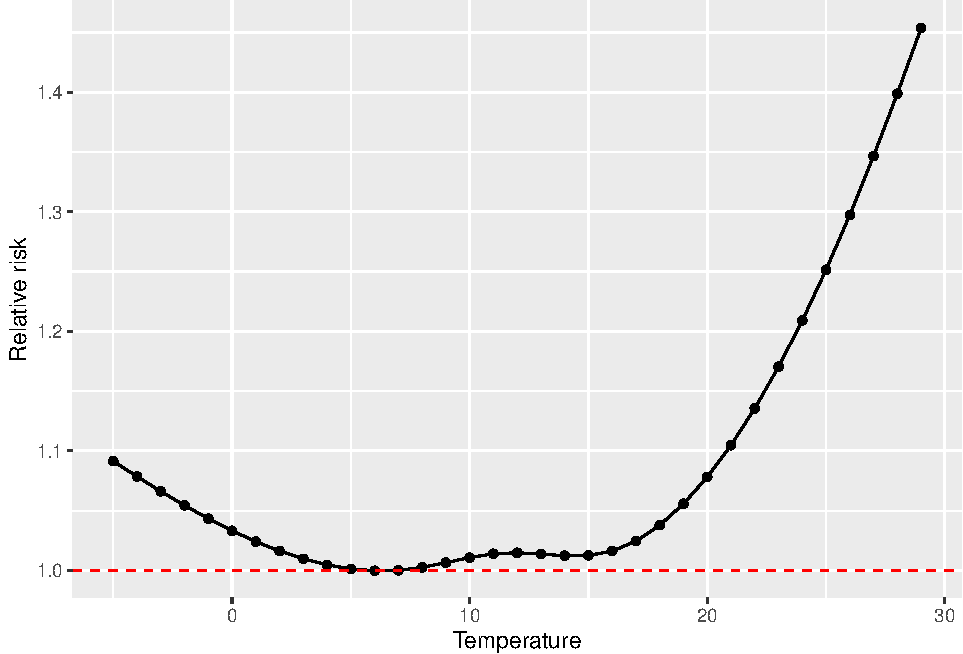
\includegraphics{adv_epi_analysis_files/figure-latex/unnamed-chunk-82-1.pdf}

The \texttt{dlnm} package also includes some functions specifically for plotting. One downside
is that they're in base R, rather than based on \texttt{ggplot2}, which makes them a bit
harder to customize. However, they're a great way to get a first look at your results:

\begin{Shaded}
\begin{Highlighting}[]
\NormalTok{dlnm\_mod\_1 }\SpecialCharTok{\%\textgreater{}\%} 
  \FunctionTok{crosspred}\NormalTok{(}\AttributeTok{basis =}\NormalTok{ temp\_basis, }\AttributeTok{model =}\NormalTok{ ., }\AttributeTok{cen =} \DecValTok{7}\NormalTok{, }\AttributeTok{by =} \DecValTok{1}\NormalTok{) }\SpecialCharTok{\%\textgreater{}\%} 
  \FunctionTok{plot}\NormalTok{()}
\end{Highlighting}
\end{Shaded}

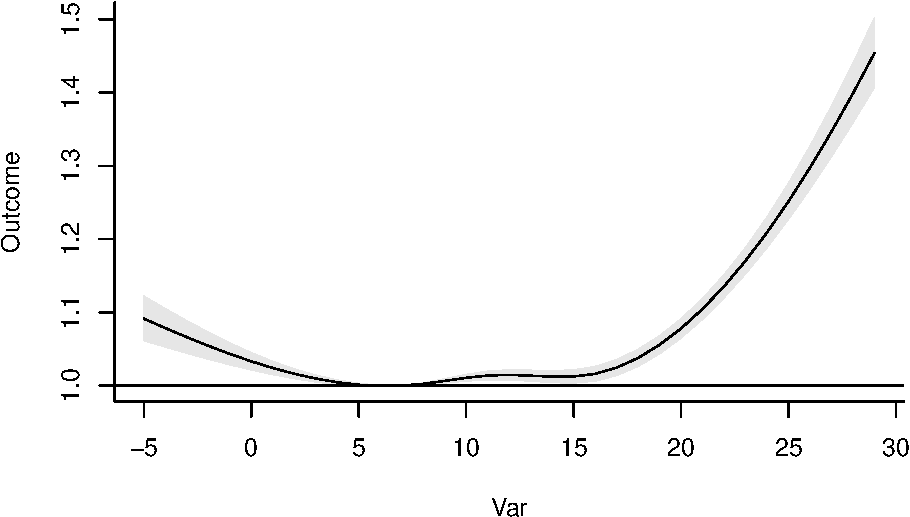
\includegraphics{adv_epi_analysis_files/figure-latex/unnamed-chunk-83-1.pdf}

Don't worry if all of this about basis functions is a lot! If this is the first time you've
seen this, it will likely take a few passes to get comfortable with it---and while the idea
of basis variables is fairly straightforward, it's certainly not straightforward to figure
out how to interpret the results of the model that you fit. It is worth the effort, though,
as this is a very powerful tool when working with regression modeling in environmental
epidemiology.

\section{Distributed lags and cross-basis functions in GLMs}\label{distributed-lags-and-cross-basis-functions-in-glms}

Next, let's explore how we can add into our model something that lets us look at
delayed effects and the potential for mortality displacement. So far, we have only
considered how temperature affects mortality risk on the day of exposure---in other
words, if it is very hot today, does risk of mortality go up substantially today?
For many exposures, however, risk can persist after the day of exposure.

In some cases, this may be caused by a delay in detection of the outcome in the
data we have. For example, extreme heat today could precipitate a respiratory or
cardiac event that the person may not seek treatment for or result in an outcome
like mortality until tomorrow, and so in the data the outcome would be recorded
at a one-day delay from the exposure.

In other cases, the path from the exposure to the outcome may take several days.
For example, cold temperatures are often found to be associated with respiratory
outcomes a week or more after exposures (something you can look for in the
example data!), and one potential pathway is that cold temperatures might
promote the spread of respiratory infectious disease, like influenza and colds,
both through making people stay inside in more crowded, less ventilated
conditions and also through effects on humidity and other conditions that might
influence the behavior of respiratory droplets, which are key players in
spreading some respiratory diseases. Since there is an incubation time up to
several days for these infectious diseases, we might expect a lagged association
between temperature and respiratory outcomes under this scenario.

There is another lagged pattern that can be important to check for, as well---one
that indicates mortality displacement. For many ambient environmental exposures,
there are clear indications that associations with health outcomes are strongest
among older adults or other populations with a disproportionately high percent
of people who are frail before exposure. One question that comes up, then, is
if, when an exposure is associated with excess deaths, these are deaths that are
displaced in time by only a few days or weeks, rather than deaths that represent
a larger time of life lost. This question---of whether deaths observed to be
associated with an environmental exposure were displaced by only a small amount of
time---can be explored by investigating whether an observed increase in mortality
across a community during an exposure is then offset by a lower-than-expected
rate of mortality in the following days and weeks.This phenomenon is sometimes
also referred to as `harvesting' or a `harvesting effect'.

All of these questions can be explored through a type of model called a
\emph{distributed lag model}. Conceptually, these models investigate how an exposure
today is associated with risk of a health outcome not only today, but also in
the following days. In time-series studies where we typically want to estimate
potential short-term and/or acute effects, and because we are concerned about potential
confounding by seasonal trends---and have incorporated control for these trends in
our models---we often restrict these models to only look up to about a month following
exposure. However, this can help in identifying delayed effects of an exposure days to weeks
following the initial exposure, and can also help in determining the role of
mortality displacement in accounting for some or all of the excess deaths that are
associated with an exposure. While some environmental exposures of interest
have mostly immediate effects (e.g., hot temperature), others, including many air
pollutants, tend to have effects that are stretched over a longer period of one or
more days from exposure. As a result, distributed lag models are used widely in
environmental epidemiology studies of time series data, to ensure that important
associations aren't missed by limiting the model to focus on risk that are
detectable on the same day as the exposure. They can also help us identify influential
windows of exposure as well as help eliminate potential confounding by exposures
occurring at proximal times to the window of interest. For example, today's exposure
may appear to have an effect on a health outcome even if in reality yesterday's
exposure is the influential one and we don't control for it, because today's and
yesterday's exposure to temperature or air pollution are likely to be very similar.

To fit a distributed lag model, you can start with a fairly straightforward
extension of the regression models we've been fitting, especially if you are
investigating an exposure that can be plausibly fit with a linear term (rather than
a more complex non-linear basis function) in the regression model. Say you are starting,
for example, from the following regression model:

\[
log(E(Y)) = \alpha + \beta X + \mathbf{\gamma^{'}W} + ns(time)
\]

In this model, you are using a Poisson regression to investigate how risk of the
health outcome (\(Y\)) changes for every unit increase in the exposure (\(X\)), assuming
a linear relationship between the exposure and the log of the health outcome. The model
can include control for confounders like day of week (\(\mathbf{W}\)) and long-term and
seasonal time trends (\(ns(time)\)). This model should look familiar from some of the
models we've fit earlier to the example temperature data.

To expand this model to explore associations of temperature at different lags, the
simplest approach is to add a term for each lag---in other words, instead of only having
a term for temperature on the same day as the outcome measurement, we'll also include a
term for temperature the previous day, and the day before that, and so on. For example,
here's what the model would look like if we included terms up to lag 2:

\[
log(E(Y)) = \alpha + \beta_{0} X_{0} + \beta_{1} X_{1} + \beta_{2} X_{2} + \mathbf{\gamma^{'}W} + ns(time)
\]
where \(X_0\) is temperature on the same day as the measured outcome \(Y\) (with an
associated coefficient \(\beta_0\)), \(X_1\) is the temperature the day before (with an
associated coefficient \(\beta_1\)), and \(X_2\) is the temperature two days before (with an
associated coefficient \(\beta_2\)). The interpretation of each of these coefficients
is similar---\(exp(\beta_2)\), for example, gives our estimate of the change in the relative
risk of the outcome \(Y\) for every one-unit increase in the exposure two days prior.

It can become cumbersome to write out the separate terms for each lag day, so you'll often
see equations for distributed lag models written using a shorter approach with the
\(\sum\) symbol. The \(\sum\) symbol expresses several terms that are added together and so
is well-suited for shortening the expression of a distributed lag model. For example, the
previous model equation could be rewritten as:

\[
log(E(Y)) = \alpha + \sum_{l=0}^2{\beta_lX_l} + \mathbf{\gamma^{'}W} + ns(time)
\]

This version of a distributed lag model is nice because it is fairly simple---we're taking the
idea of fitting a linear term for an exposure, and then expanding it to include the
exposure on earlier days by adding the same type of term for exposure measured at each lag.
However, it does have some downsides. The main downside is that exposure
tends to be very strongly correlated from one day to the next. Any time you put different terms in a regression model that are correlated, you create the risk of \emph{collinearity}, and associated
problems with fitting the model. The term \emph{collinearity} refers to the idea that you have two or more
columns in your model matrix that give identical (or, if you loosen the definition a bit,
very similar) information. To fit coefficients for each term, the modeling algorithm is trying
to identify weights to place on each column in the model matrix that result in a model that
gives the best likelihood of the data you see. If two or more columns have (almost) identical
information, then the algorithm struggles to determine how to distribute weight across these
two columns. The implications are that you can end up with a lot of instability in model
coefficients for the columns that are collinear, as well as very inflated estimates of the
standard error. Long story short, it can cause problems in your regression model if you include
independent variables that are very strongly correlated with each other, and so we usually
try to avoid doing that.

There are alternative distributed lag models that can help avoid this instability that can
arise from fitting a distributed lag by using a separate term for each lag. All of them share
a common feature---they somehow fit a function of the lags instead of each separate lag, so
that we end up adding fewer terms to the regression model (and, in turn, are somewhat
constraining the pattern that the distributed lag effects follow). At the most extreme,
you can use a function that reduces all the lag terms to a single term, which you can do by
averaging the exposure across all lags. In other words, you could take the same-day
temperature, yesterday's temperature, and the temperature the day before that, and average
those three temperatures to create the term you put in the model. The model equation
in this case would look like:

\[
log(E(Y)) = \alpha + \beta_{\overline{0-2}} X_{\overline{0-2}} + \mathbf{\gamma^{'}W} + ns(time)
\]
where \(\overline{0-2}\) represents an average over lags 0 to 2, and so \(X_{\overline{0-2}}\)
is the average of the exposure on lags 0, 1, and 2 compared to the day that \(Y\) is
measured.

This approach avoids any issues with collinearity across exposure terms from different
lags, because you're only including a single term for exposure in the model. However,
there is a downside---this model will provide you with a single estimate for the
lagged effects, without allowing you to explore patterns across lags (for example,
is the association mostly on the day of exposure, or are there some delayed effects on
following days?). Instead, the main assumption is that the effect is constant across
all days in the window of interest.

Another approach is more complex, but it allows you to explore patterns across lags.
Instead of reducing the lagged exposure to a single term in the model, you can reduce
it to a few terms that represent the basis for a smooth function. Often, a polynomial
or natural cubic spline function will be used for this. The details of setting up the
model become more complex, but fortunately there are software packages (like the \texttt{dlnm}
package in R) that help in managing this set-up, as we'll explore in the exercise.

Packages like \texttt{dlnm} can help in extending the complexity of the distributed lag model
in other ways, too. So far, we have explored using a distributed lag model where we
are happy to model the exposure using a linear term. As we've seen in earlier exercises,
this isn't ideal for temperature. Instead, temperature has a non-linear association
with mortality risk, with the lowest risk at mild temperatures and then increased risk
at both lower (colder) and higher (hotter) temperatures.

We can fit a GLM that incorporates the exposure using a non-linear shape while, at the
same time, including a non-linear function to describe how the association evolves
across lagged time following the exposure. The approach is to extend the idea of
using a basis function---instead of using a basis function in a single dimension, we'll
use a cross of basis functions in two dimensions. One dimension is the level of exposure
(e.g., cold to hot temperatures), and the other is the timing between the exposure and
the outcome (e.g., same-day to lagged by many days). In terms of the mechanics of
building a model matrix to use to fit the regression model, everything follows directly
from the idea we explored earlier of using a function like a spline to create basis
variables in that model matrix for a term with a non-linear association with the
outcome variable. However, the mechanics do get quite cumbersome as so many terms are
included, and so again we will use the \texttt{dlnm} package to handle these mechanics as we
start to incorporate these cross-basis functions within a GLM.

\emph{Applied: Including a cross-basis function for exposure-lag-response in a GLM}

For this exercise, you will continue to build up the model that you began in
the examples in the previous chapter. The example uses the data provided with
one of this chapter's readings, \citet{vicedo2019hands}.

\begin{enumerate}
\def\labelenumi{\arabic{enumi}.}
\tightlist
\item
  Start with the simple model describing how are daily mortality counts are
  associated with a linear function of temperature. Include control for day of
  week and long-term / seasonal trends. Add to this model a term that describes
  the lagged effects of temperature up to a week following exposure, using a
  separate model term for each lag. What patterns do you detect in the lagged
  effects of temperature?
\item
  Start with the model from the first question, but change it to use a smooth
  function of lag to detect lagged effects, rather than fitting a seperate term
  for each lag. Extend the model to look at lagged effects up to a month following
  exposure. What patterns do you see in these lagged effects?
\item
  Refine your model to fit for a non-linear, rather than linear, function
  of temperature, while also incorporating a function to describe lagged effects up
  to a month following exposure. Based on this model, what does the association
  between temperature and mortality look like at lag 0 days? How about at lag 21 days?
  What does the pattern of lagged effects look like when comparing the relative risk of
  mortality at a hot temperature (e.g., 28 degrees C) to a milder temperature
  (7 degrees C)? What about when comparing mortality at a cold temperature
  (e.g., -4 degrees C) to a milder temperature (7 degrees C)? If you use a constant
  term for the effect of exposure
  over a month as opposed to the smooth function you just used, how does the overall
  cumulative RR compare?
\item
  Assume that we are interested in the potential effect of a 5-day
  heatwave occurring on lags 0 to 4? You can assess this as the effect of hot temperature
  (e.g., 28 degrees C) during these lags, while the temperature remains warm but more
  mild (e.g., 20 degrees C) the rest of the month, against constant 20 degrees C for
  the whole month. What is the effect under the `constant' model? How about the smooth
  function lag model?
\end{enumerate}

\emph{Applied exercise: Example code}

\begin{enumerate}
\def\labelenumi{\arabic{enumi}.}
\tightlist
\item
  \textbf{Start with the simple model describing how are daily mortality counts are
  associated with a linear function of temperature. Include control for day of
  week and long-term / seasonal trends. Add to this model a term that describes
  the lagged effects of temperature up to a week following exposure, using a
  separate model term for each lag. What patterns do you detect in the lagged
  effects of temperature?}
\end{enumerate}

We'll start by looking at distributed lag associations by fitting a model with
separate terms for each of the lags we want to fit. Here, we want to fit up to
a week, so we'll want eight terms in total: ones for the same day (\(X_0\)), the
previous day (\(X_1\)), two days before (\(X_2\)), three days before (\(X_3\)),
four days before (\(X_4\)), five days before (\(X_5\)), six days before (\(X_6\)),
and seven days before (\(X_7\)).

Right now, our data have temperature lined up with the date of the recorded deaths:

\begin{Shaded}
\begin{Highlighting}[]
\NormalTok{obs }\SpecialCharTok{\%\textgreater{}\%} 
  \FunctionTok{select}\NormalTok{(date, all, tmean) }\SpecialCharTok{\%\textgreater{}\%} 
  \FunctionTok{head}\NormalTok{()}
\end{Highlighting}
\end{Shaded}

\begin{verbatim}
## # A tibble: 6 x 3
##   date         all tmean
##   <date>     <dbl> <dbl>
## 1 1990-01-01   220  3.91
## 2 1990-01-02   257  5.55
## 3 1990-01-03   245  4.39
## 4 1990-01-04   226  5.43
## 5 1990-01-05   236  6.87
## 6 1990-01-06   235  9.23
\end{verbatim}

To add lagged temperature to the model, then, we'll need to add some columns to our
data, so that the row for an observation includes not only the temperature on that
day, but also on each of the seven previous days. The \texttt{lag} function from the \texttt{tidyverse}
suite of packages can be used to create these columns:

\begin{Shaded}
\begin{Highlighting}[]
\NormalTok{obs }\OtherTok{\textless{}{-}}\NormalTok{ obs }\SpecialCharTok{\%\textgreater{}\%} 
  \FunctionTok{mutate}\NormalTok{(}\AttributeTok{tmean\_1 =} \FunctionTok{lag}\NormalTok{(tmean, }\AttributeTok{n =} \DecValTok{1}\NormalTok{), }
         \AttributeTok{tmean\_2 =} \FunctionTok{lag}\NormalTok{(tmean, }\AttributeTok{n =} \DecValTok{2}\NormalTok{), }
         \AttributeTok{tmean\_3 =} \FunctionTok{lag}\NormalTok{(tmean, }\AttributeTok{n =} \DecValTok{3}\NormalTok{), }
         \AttributeTok{tmean\_4 =} \FunctionTok{lag}\NormalTok{(tmean, }\AttributeTok{n =} \DecValTok{4}\NormalTok{), }
         \AttributeTok{tmean\_5 =} \FunctionTok{lag}\NormalTok{(tmean, }\AttributeTok{n =} \DecValTok{5}\NormalTok{), }
         \AttributeTok{tmean\_6 =} \FunctionTok{lag}\NormalTok{(tmean, }\AttributeTok{n =} \DecValTok{6}\NormalTok{), }
         \AttributeTok{tmean\_7 =} \FunctionTok{lag}\NormalTok{(tmean, }\AttributeTok{n =} \DecValTok{7}\NormalTok{))}
\end{Highlighting}
\end{Shaded}

You can see below that each of these have taken \texttt{tmean} and then offset it by moving it down
by one or more rows (down one row for lag 1, two for lag 2, etc.). As a result, we now have
columns that give us today's temperature, yesterday's, and so on, all lined up with the
row with the observation for daily mortality:

\begin{Shaded}
\begin{Highlighting}[]
\NormalTok{obs }\SpecialCharTok{\%\textgreater{}\%} 
  \FunctionTok{select}\NormalTok{(date, all, tmean, tmean\_1}\SpecialCharTok{:}\NormalTok{tmean\_7) }\SpecialCharTok{\%\textgreater{}\%} 
  \FunctionTok{head}\NormalTok{()}
\end{Highlighting}
\end{Shaded}

\begin{verbatim}
## # A tibble: 6 x 10
##   date         all tmean tmean_1 tmean_2 tmean_3 tmean_4 tmean_5 tmean_6 tmean_7
##   <date>     <dbl> <dbl>   <dbl>   <dbl>   <dbl>   <dbl>   <dbl>   <dbl>   <dbl>
## 1 1990-01-01   220  3.91   NA      NA      NA      NA      NA         NA      NA
## 2 1990-01-02   257  5.55    3.91   NA      NA      NA      NA         NA      NA
## 3 1990-01-03   245  4.39    5.55    3.91   NA      NA      NA         NA      NA
## 4 1990-01-04   226  5.43    4.39    5.55    3.91   NA      NA         NA      NA
## 5 1990-01-05   236  6.87    5.43    4.39    5.55    3.91   NA         NA      NA
## 6 1990-01-06   235  9.23    6.87    5.43    4.39    5.55    3.91      NA      NA
\end{verbatim}

You'll notice that this process has created some missing data right at the beginning of the
dataset---we don't know what the temperature was the day before Jan.~1, 1990, for example,
since the study data starts on Jan.~1, 1990. With most time series, we'll have plenty of
days in the study period, so we'll usually just allow these early dates to drop when the
model is fit.

Now we'll add all these terms to our regression model:

\begin{Shaded}
\begin{Highlighting}[]
\NormalTok{dist\_lag\_mod\_1 }\OtherTok{\textless{}{-}} \FunctionTok{glm}\NormalTok{(all }\SpecialCharTok{\textasciitilde{}}\NormalTok{ tmean }\SpecialCharTok{+}\NormalTok{ tmean\_1 }\SpecialCharTok{+}\NormalTok{ tmean\_2 }\SpecialCharTok{+}\NormalTok{ tmean\_3 }\SpecialCharTok{+}\NormalTok{ tmean\_4 }\SpecialCharTok{+} 
\NormalTok{                        tmean\_5 }\SpecialCharTok{+}\NormalTok{ tmean\_6 }\SpecialCharTok{+}\NormalTok{ tmean\_7 }\SpecialCharTok{+} 
                        \FunctionTok{factor}\NormalTok{(dow, }\AttributeTok{ordered =} \ConstantTok{FALSE}\NormalTok{) }\SpecialCharTok{+}
                          \FunctionTok{ns}\NormalTok{(time, }\AttributeTok{df =} \DecValTok{158}\NormalTok{), }
                        \AttributeTok{data =}\NormalTok{ obs, }\AttributeTok{family =} \StringTok{"quasipoisson"}\NormalTok{)}
\end{Highlighting}
\end{Shaded}

If you look at the output from the model, you can see that a regression coefficient has been
fit for each of these distributed lag terms:

\begin{Shaded}
\begin{Highlighting}[]
\NormalTok{dist\_lag\_mod\_1 }\SpecialCharTok{\%\textgreater{}\%} 
  \FunctionTok{tidy}\NormalTok{() }\SpecialCharTok{\%\textgreater{}\%} 
  \FunctionTok{filter}\NormalTok{(}\FunctionTok{str\_detect}\NormalTok{(term, }\StringTok{"tmean"}\NormalTok{))}
\end{Highlighting}
\end{Shaded}

\begin{verbatim}
## # A tibble: 8 x 5
##   term     estimate std.error statistic  p.value
##   <chr>       <dbl>     <dbl>     <dbl>    <dbl>
## 1 tmean    0.00749   0.000592    12.6   2.67e-36
## 2 tmean_1 -0.00255   0.000788    -3.23  1.25e- 3
## 3 tmean_2 -0.00152   0.000797    -1.91  5.68e- 2
## 4 tmean_3 -0.00243   0.000798    -3.05  2.31e- 3
## 5 tmean_4 -0.00106   0.000798    -1.32  1.86e- 1
## 6 tmean_5 -0.000515  0.000797    -0.645 5.19e- 1
## 7 tmean_6 -0.00107   0.000789    -1.36  1.73e- 1
## 8 tmean_7 -0.00209   0.000593    -3.52  4.30e- 4
\end{verbatim}

We can pull out all those estimates, calculate the 95\% confidence intervals (do this \emph{before}
you take the exponential to get to the relative risk estimate, not after!), and then
exponentiate all the terms to get estimates of relative risk of mortality per unit increase
in temperature.

\begin{Shaded}
\begin{Highlighting}[]
\NormalTok{dist\_lag\_terms }\OtherTok{\textless{}{-}}\NormalTok{ dist\_lag\_mod\_1 }\SpecialCharTok{\%\textgreater{}\%} 
  \FunctionTok{tidy}\NormalTok{() }\SpecialCharTok{\%\textgreater{}\%} 
  \FunctionTok{filter}\NormalTok{(}\FunctionTok{str\_detect}\NormalTok{(term, }\StringTok{"tmean"}\NormalTok{)) }\SpecialCharTok{\%\textgreater{}\%} 
  \FunctionTok{mutate}\NormalTok{(}\AttributeTok{lag =} \DecValTok{0}\SpecialCharTok{:}\DecValTok{7}\NormalTok{, }
         \AttributeTok{low\_ci =}\NormalTok{ estimate }\SpecialCharTok{{-}} \FloatTok{1.96} \SpecialCharTok{*}\NormalTok{ std.error, }
         \AttributeTok{high\_ci =}\NormalTok{ estimate }\SpecialCharTok{+} \FloatTok{1.96} \SpecialCharTok{*}\NormalTok{ std.error, }
         \AttributeTok{rr =} \FunctionTok{exp}\NormalTok{(estimate), }
         \AttributeTok{low\_rr =} \FunctionTok{exp}\NormalTok{(low\_ci), }
         \AttributeTok{high\_rr =} \FunctionTok{exp}\NormalTok{(high\_ci)) }\SpecialCharTok{\%\textgreater{}\%} 
  \FunctionTok{select}\NormalTok{(term, lag, rr, low\_rr, high\_rr)}
\NormalTok{dist\_lag\_terms}
\end{Highlighting}
\end{Shaded}

\begin{verbatim}
## # A tibble: 8 x 5
##   term      lag    rr low_rr high_rr
##   <chr>   <int> <dbl>  <dbl>   <dbl>
## 1 tmean       0 1.01   1.01    1.01 
## 2 tmean_1     1 0.997  0.996   0.999
## 3 tmean_2     2 0.998  0.997   1.00 
## 4 tmean_3     3 0.998  0.996   0.999
## 5 tmean_4     4 0.999  0.997   1.00 
## 6 tmean_5     5 0.999  0.998   1.00 
## 7 tmean_6     6 0.999  0.997   1.00 
## 8 tmean_7     7 0.998  0.997   0.999
\end{verbatim}

You can plot these estimates to explore how the association changes by lag (notice how
\texttt{geom\_pointrange} is very helpful here!):

\begin{Shaded}
\begin{Highlighting}[]
\NormalTok{dist\_lag\_terms }\SpecialCharTok{\%\textgreater{}\%} 
  \FunctionTok{ggplot}\NormalTok{(}\FunctionTok{aes}\NormalTok{(}\AttributeTok{x =}\NormalTok{ lag, }\AttributeTok{y =}\NormalTok{ rr)) }\SpecialCharTok{+} 
  \FunctionTok{geom\_point}\NormalTok{() }\SpecialCharTok{+} 
  \FunctionTok{geom\_pointrange}\NormalTok{(}\FunctionTok{aes}\NormalTok{(}\AttributeTok{ymin =}\NormalTok{ low\_rr, }\AttributeTok{ymax =}\NormalTok{ high\_rr)) }\SpecialCharTok{+} 
  \FunctionTok{labs}\NormalTok{(}\AttributeTok{x =} \StringTok{"Lag days since exposure"}\NormalTok{, }
       \AttributeTok{y =} \StringTok{"Relative risk of mortality}\SpecialCharTok{\textbackslash{}n}\StringTok{per degree increase in temperature"}\NormalTok{) }\SpecialCharTok{+} 
  \FunctionTok{geom\_hline}\NormalTok{(}\AttributeTok{yintercept =} \DecValTok{1}\NormalTok{, }\AttributeTok{color =} \StringTok{"red"}\NormalTok{, }\AttributeTok{linetype =} \DecValTok{3}\NormalTok{)}
\end{Highlighting}
\end{Shaded}

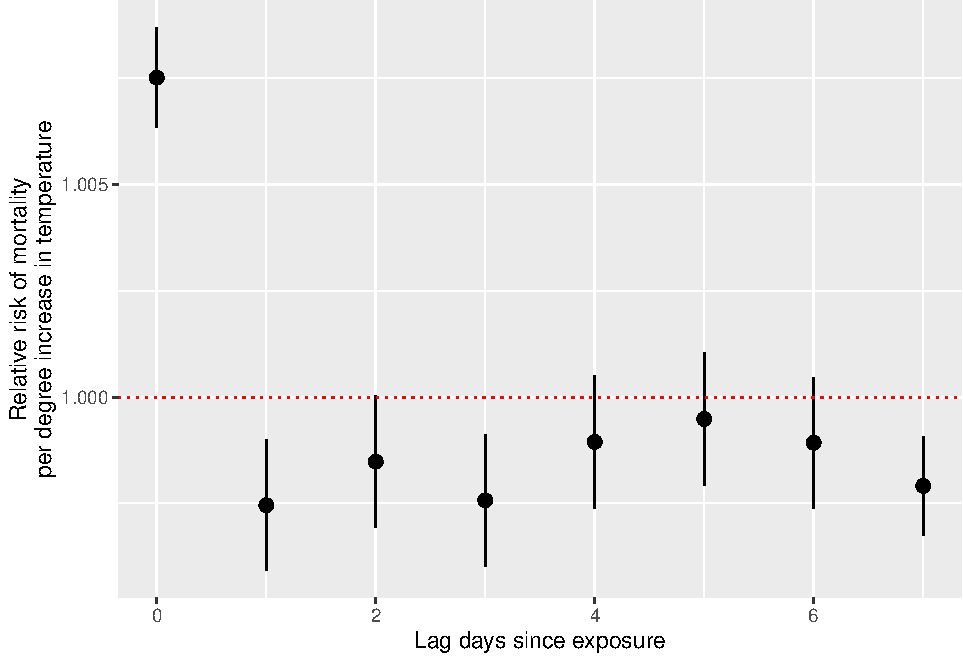
\includegraphics{adv_epi_analysis_files/figure-latex/unnamed-chunk-90-1.pdf}

You can also, as an alternative, use the \texttt{dlnm} package to fit this
model, using the \texttt{crossbasis} function
to set up the distributed lag basis to include in the regression, and then the \texttt{crosspred}
function to extract results after fitting the regression model and to plot results.

First, you'll again use \texttt{crossbasis} to create the basis, as you did earlier when using this
package to fit a non-linear function of temperature. You will use the \texttt{lag} argument to say
the maximum lag you want to include---in this case, seven days (\texttt{lag\ =\ 7}). You can use
the \texttt{argvar} and \texttt{arglag} functions to specify the basis function for the exposure variable
and the distributed lag component. For right now, we'll use a very basic linear function for
the exposure (temperature), using \texttt{fun\ =\ "lin"} within the \texttt{argvar} list of arguments.
To fit a separate coefficient for each lag, we can specify \texttt{fun\ =\ "integer"} in the
\texttt{arglag} list of arguments (later we'll explore some other functions for the lag component).

\begin{Shaded}
\begin{Highlighting}[]
\FunctionTok{library}\NormalTok{(dlnm)}
\NormalTok{dl\_basis }\OtherTok{\textless{}{-}} \FunctionTok{crossbasis}\NormalTok{(obs}\SpecialCharTok{$}\NormalTok{tmean, }\AttributeTok{lag =} \DecValTok{7}\NormalTok{,}
                       \AttributeTok{argvar =} \FunctionTok{list}\NormalTok{(}\AttributeTok{fun =} \StringTok{"lin"}\NormalTok{), }
                       \AttributeTok{arglag =} \FunctionTok{list}\NormalTok{(}\AttributeTok{fun =} \StringTok{"integer"}\NormalTok{))}
\end{Highlighting}
\end{Shaded}

If you take a peak at this crossbasis, you'll notice that it's doing something similar to
what we did when we added columns for lagged temperatures. The first column gives temperature
on the same day, the second on the previous day (and so is offset one down from the first
column), and so on. The crossbasis function deals with the missing early dates by setting
\emph{all} column values to be missing on those days; in practice, this difference in set up
won't create any difference in how the model is fit, as the \texttt{glm} function will by default
exclude any observations with \emph{any} columns of missing data.

\begin{Shaded}
\begin{Highlighting}[]
\NormalTok{dl\_basis }\SpecialCharTok{\%\textgreater{}\%} 
  \FunctionTok{head}\NormalTok{(}\AttributeTok{n =} \DecValTok{12}\NormalTok{)}
\end{Highlighting}
\end{Shaded}

\begin{verbatim}
##           v1.l1     v1.l2    v1.l3    v1.l4    v1.l5    v1.l6    v1.l7    v1.l8
##  [1,]        NA        NA       NA       NA       NA       NA       NA       NA
##  [2,]        NA        NA       NA       NA       NA       NA       NA       NA
##  [3,]        NA        NA       NA       NA       NA       NA       NA       NA
##  [4,]        NA        NA       NA       NA       NA       NA       NA       NA
##  [5,]        NA        NA       NA       NA       NA       NA       NA       NA
##  [6,]        NA        NA       NA       NA       NA       NA       NA       NA
##  [7,]        NA        NA       NA       NA       NA       NA       NA       NA
##  [8,]  7.958644  6.686216 9.232628 6.867855 5.431046 4.385564 5.547919 3.913589
##  [9,]  7.268950  7.958644 6.686216 9.232628 6.867855 5.431046 4.385564 5.547919
## [10,]  9.510644  7.268950 7.958644 6.686216 9.232628 6.867855 5.431046 4.385564
## [11,] 10.424808  9.510644 7.268950 7.958644 6.686216 9.232628 6.867855 5.431046
## [12,]  7.368595 10.424808 9.510644 7.268950 7.958644 6.686216 9.232628 6.867855
\end{verbatim}

We can use this matrix of crossbasis variables now in our regression call:

\begin{Shaded}
\begin{Highlighting}[]
\NormalTok{dist\_lag\_mod\_2 }\OtherTok{\textless{}{-}} \FunctionTok{glm}\NormalTok{(all }\SpecialCharTok{\textasciitilde{}}\NormalTok{ dl\_basis }\SpecialCharTok{+} 
                        \FunctionTok{factor}\NormalTok{(dow, }\AttributeTok{ordered =} \ConstantTok{FALSE}\NormalTok{) }\SpecialCharTok{+}
                          \FunctionTok{ns}\NormalTok{(time, }\AttributeTok{df =} \DecValTok{158}\NormalTok{), }
                        \AttributeTok{data =}\NormalTok{ obs, }\AttributeTok{family =} \StringTok{"quasipoisson"}\NormalTok{)}
\end{Highlighting}
\end{Shaded}

Again, you can pull the regression coefficients directly out of the regression model object
(and you can see how they're identical to those from our first distributed lag model):

\begin{Shaded}
\begin{Highlighting}[]
\NormalTok{dist\_lag\_mod\_2 }\SpecialCharTok{\%\textgreater{}\%} 
  \FunctionTok{tidy}\NormalTok{() }\SpecialCharTok{\%\textgreater{}\%} 
  \FunctionTok{filter}\NormalTok{(}\FunctionTok{str\_detect}\NormalTok{(term, }\StringTok{"dl\_basis"}\NormalTok{))}
\end{Highlighting}
\end{Shaded}

\begin{verbatim}
## # A tibble: 8 x 5
##   term           estimate std.error statistic  p.value
##   <chr>             <dbl>     <dbl>     <dbl>    <dbl>
## 1 dl_basisv1.l1  0.00749   0.000592    12.6   2.67e-36
## 2 dl_basisv1.l2 -0.00255   0.000788    -3.23  1.25e- 3
## 3 dl_basisv1.l3 -0.00152   0.000797    -1.91  5.68e- 2
## 4 dl_basisv1.l4 -0.00243   0.000798    -3.05  2.31e- 3
## 5 dl_basisv1.l5 -0.00106   0.000798    -1.32  1.86e- 1
## 6 dl_basisv1.l6 -0.000515  0.000797    -0.645 5.19e- 1
## 7 dl_basisv1.l7 -0.00107   0.000789    -1.36  1.73e- 1
## 8 dl_basisv1.l8 -0.00209   0.000593    -3.52  4.30e- 4
\end{verbatim}

You can proceed from here to plot estimates by lag using ggplot, but you can also use
some of the special functions for plotting in \texttt{dlnm}. We can plot the ``slice'' of comparing
the relative risk at 1 degree C (\texttt{var\ =\ 1}) (this will give us the one-unit increase,
because by default the crossbasis set-up with 0 degrees as the baseline, so this is
one degree above that value). The \texttt{crosspred} function predicts based on two things: (1)
a crossbasis and (2) a regression model object that uses that crossbasis. Once you create
an object with \texttt{crosspred}, then the \texttt{plot} function has a
special method for plotting that object (to see the helpfile for this
plot method, type \texttt{?plot.crosspred} in your R console).

\begin{Shaded}
\begin{Highlighting}[]
\FunctionTok{crosspred}\NormalTok{(dl\_basis, dist\_lag\_mod\_2) }\SpecialCharTok{\%\textgreater{}\%} 
  \FunctionTok{plot}\NormalTok{(}\AttributeTok{ptype =} \StringTok{"slices"}\NormalTok{, }\AttributeTok{var =} \DecValTok{1}\NormalTok{, }\AttributeTok{ci =} \StringTok{"bars"}\NormalTok{)}
\end{Highlighting}
\end{Shaded}

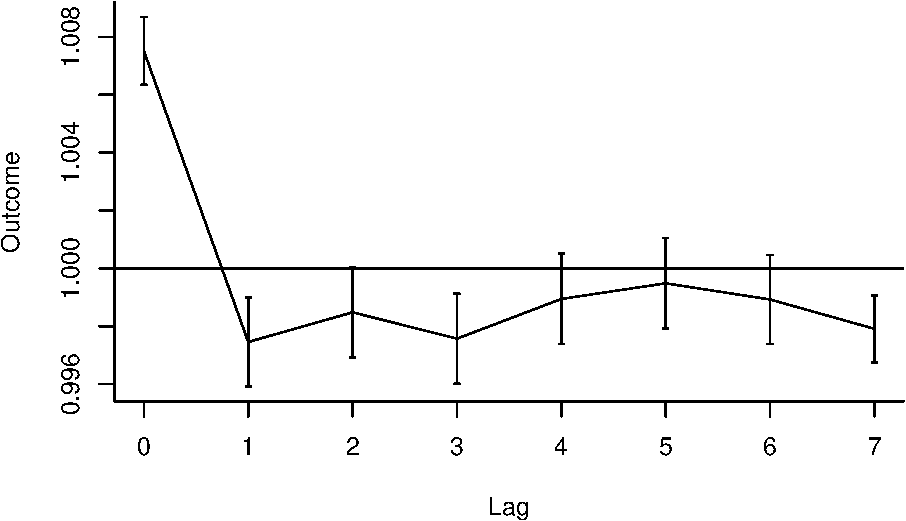
\includegraphics{adv_epi_analysis_files/figure-latex/unnamed-chunk-95-1.pdf}

However, even though mechanically we can fit this model, we should think about whether
it's a good idea, or whether we should contrain the lag function some.
If you look at the correlations between temperature at different lags, you'll see they are very
strongly correlated:

\begin{Shaded}
\begin{Highlighting}[]
\NormalTok{obs }\SpecialCharTok{\%\textgreater{}\%} 
  \FunctionTok{select}\NormalTok{(tmean, tmean\_1}\SpecialCharTok{:}\NormalTok{tmean\_7) }\SpecialCharTok{\%\textgreater{}\%} 
  \FunctionTok{cor}\NormalTok{(}\AttributeTok{use =} \StringTok{"complete.obs"}\NormalTok{) }
\end{Highlighting}
\end{Shaded}

\begin{verbatim}
##             tmean   tmean_1   tmean_2   tmean_3   tmean_4   tmean_5   tmean_6
## tmean   1.0000000 0.9431416 0.8845767 0.8462589 0.8215974 0.8031790 0.7891306
## tmean_1 0.9431416 1.0000000 0.9431447 0.8846236 0.8463419 0.8216464 0.8032469
## tmean_2 0.8845767 0.9431447 1.0000000 0.9431403 0.8846198 0.8463094 0.8216348
## tmean_3 0.8462589 0.8846236 0.9431403 1.0000000 0.9431414 0.8846132 0.8463072
## tmean_4 0.8215974 0.8463419 0.8846198 0.9431414 1.0000000 0.9431482 0.8846132
## tmean_5 0.8031790 0.8216464 0.8463094 0.8846132 0.9431482 1.0000000 0.9431506
## tmean_6 0.7891306 0.8032469 0.8216348 0.8463072 0.8846132 0.9431506 1.0000000
## tmean_7 0.7781337 0.7892093 0.8032205 0.8216271 0.8463046 0.8846283 0.9431482
##           tmean_7
## tmean   0.7781337
## tmean_1 0.7892093
## tmean_2 0.8032205
## tmean_3 0.8216271
## tmean_4 0.8463046
## tmean_5 0.8846283
## tmean_6 0.9431482
## tmean_7 1.0000000
\end{verbatim}

This means that we could have some issues with collinearity if we
use this simpler distributed lag model, with a separate coefficient for each lag
Next, we'll explore a model that constrains the lagged effects to follow a smooth
function, to help avoid this potential instability in the modeling.

\begin{enumerate}
\def\labelenumi{\arabic{enumi}.}
\setcounter{enumi}{1}
\tightlist
\item
  \textbf{Start with the model from the first question, but change it to use a smooth
  function of lag to detect lagged effects, rather than fitting a separate term
  for each lag. Extend the model to look at lagged effects up to a month following
  exposure. What patterns do you see in these lagged effects?}
\end{enumerate}

As a reminder, we can stabilize our model of lagged effects a bit by fitting the
lagged effects to be constrained to follow a smooth function, instead of fitting a separate
term for each lag. The \texttt{dlnm} package makes this very easy to do.

When you use \texttt{crossbasis} to set up a crossbasis function, you can make a lot of choices
to customize that crossbasis. The crossbasis combines a basis function for incorporating
the exposure in the regression model (temperature in this case), as well as a basis function
for incorporating lagged effects of that exposure. The \texttt{crossbasis} functions gives you
several choices for each of these basis functions for the two dimensions of the
crossbasis. Here, we'll look at using that flexibility for the lag dimension; in the next
part of the exercise, we'll add some more complexity in the basis function for the
exposure, as well.

To customize the basis function for lagged effects, you can use the \texttt{arglag} parameter
in the \texttt{crossbasis} function. You send this parameter a list of other parameters, which
get sent to a general \texttt{onebasis} function that builds that basis function (this will
be convenient when we start working with the exposure basis, too---you'll see that you
can use the same parameters in setting up each basis function).

To see the range of functions you can use for this crossbasis function, check the help
function for \texttt{onebasis}. When we fit a separate coefficient for each lag, we used the
``integer'' function, which creates a set of basis variables with indicators for each
separate lag (this is really similar to the idea of basis variables for a categorical
variable, like day of the week). This is what we did in the first part of the exercise.

Now, we want to instead use a smooth function, with fewer degrees of freedom (i.e., fewer
columns created in the matrix of basis values). Two popular options for that function are
the ``poly'' function, which will fit a polynomial, or the ``ns'' function, which will fit
a natural cubic spline (just like we did earlier to create a non-linear function of
temperature). We'll use ``ns'' in this example (\texttt{fun\ =\ "ns"} in the list of parameters for
\texttt{arglag}).

For some of these functions, you'll need to specify additional parameters to clarify
how they should be built. For example, if you're using a spline, you need to specify
how many degrees of freedom it should have with \texttt{df}. We'll use 4 degrees of freedom,
but you can experiment with different values for this and see how it affects the shape
of the resulting function (i.e., the plot we create later). If you were fitting a
polynomial function,
you'd need to specify the degree of the polynomial; if you were fitting strata (i.e.,
constant values within sets of lags), you'd need to specify the breaks for dividing
those strata; if you were using a threshold function, you'd need to specify the threshold,
and so on. You can find more details on these options in the helpfile for \texttt{onebasis};
in general, the \texttt{onebasis} function is using other underlying functions like \texttt{ns} and
\texttt{poly} to build these functions, so the choice of parameters will depend on the parameters
for those underlying functions.

Here is the final call for building this new crossbasis (note that we're continuing to
use a linear function of temperature, and at this point still only looking at lags up to
a week; later in this question we'll expand to look at longer lags):

\begin{Shaded}
\begin{Highlighting}[]
\NormalTok{dl\_basis\_2 }\OtherTok{\textless{}{-}} \FunctionTok{crossbasis}\NormalTok{(obs}\SpecialCharTok{$}\NormalTok{tmean, }\AttributeTok{lag =} \DecValTok{7}\NormalTok{,}
                       \AttributeTok{argvar =} \FunctionTok{list}\NormalTok{(}\AttributeTok{fun =} \StringTok{"lin"}\NormalTok{), }
                       \AttributeTok{arglag =} \FunctionTok{list}\NormalTok{(}\AttributeTok{fun =} \StringTok{"ns"}\NormalTok{, }\AttributeTok{df =} \DecValTok{4}\NormalTok{))}
\end{Highlighting}
\end{Shaded}

If you look at this crossbasis object, you'll see that it's created a matrix of basis
variables, similar to the last part of the exercise. However, instead of having the same
number of columns as the number of lags (8), we now have fewer columns. We have 4, reflecting
the degrees of freedom we specified for the spline function of lag. Therefore, we've
constrained the lag function a bit compared to the previous part of the exercise. Again,
the values are all missing for the first seven days, since the data isn't able to capture
the lagged temperature for these days.

\begin{Shaded}
\begin{Highlighting}[]
\NormalTok{dl\_basis\_2 }\SpecialCharTok{\%\textgreater{}\%} 
  \FunctionTok{head}\NormalTok{(}\AttributeTok{n =} \DecValTok{12}\NormalTok{)}
\end{Highlighting}
\end{Shaded}

\begin{verbatim}
##          v1.l1    v1.l2    v1.l3      v1.l4
##  [1,]       NA       NA       NA         NA
##  [2,]       NA       NA       NA         NA
##  [3,]       NA       NA       NA         NA
##  [4,]       NA       NA       NA         NA
##  [5,]       NA       NA       NA         NA
##  [6,]       NA       NA       NA         NA
##  [7,]       NA       NA       NA         NA
##  [8,] 10.53142 5.938107 17.26767 -2.9117904
##  [9,] 11.46186 7.311815 17.99659 -2.0873124
## [10,] 10.91751 8.769682 19.69413 -3.2804334
## [11,] 10.94122 8.867758 22.33138 -2.7169313
## [12,] 13.00391 8.984807 22.20899 -0.3726342
\end{verbatim}

Again, once we build the crossbasis function, we can put it in the regression equation and
fit a regression model using \texttt{glm}:

\begin{Shaded}
\begin{Highlighting}[]
\NormalTok{dist\_lag\_mod\_3 }\OtherTok{\textless{}{-}} \FunctionTok{glm}\NormalTok{(all }\SpecialCharTok{\textasciitilde{}}\NormalTok{ dl\_basis\_2 }\SpecialCharTok{+} 
                        \FunctionTok{factor}\NormalTok{(dow, }\AttributeTok{ordered =} \ConstantTok{FALSE}\NormalTok{) }\SpecialCharTok{+}
                          \FunctionTok{ns}\NormalTok{(time, }\AttributeTok{df =} \DecValTok{158}\NormalTok{), }
                        \AttributeTok{data =}\NormalTok{ obs, }\AttributeTok{family =} \StringTok{"quasipoisson"}\NormalTok{)}
\end{Highlighting}
\end{Shaded}

Again, you can plot the results to see the pattern of associations by lag. The plot
is just visualizing the results of predicting the model to certain values. By default,
it will predict at each lag; this makes the plot a little ``jumpy'' if you're just looking
at lags for a week or so, so to make it smoother, you might want to ask \texttt{crosspred} to
predict to a finer resolution along the lag dimension (here, we're using \texttt{bylag\ =\ 0.2}).

\begin{Shaded}
\begin{Highlighting}[]
\FunctionTok{crosspred}\NormalTok{(dl\_basis\_2, dist\_lag\_mod\_3, }\AttributeTok{at =} \DecValTok{1}\NormalTok{, }\AttributeTok{bylag =} \FloatTok{0.2}\NormalTok{) }\SpecialCharTok{\%\textgreater{}\%} 
  \FunctionTok{plot}\NormalTok{(}\AttributeTok{ptype =} \StringTok{"slices"}\NormalTok{, }\AttributeTok{var =} \DecValTok{1}\NormalTok{)}
\end{Highlighting}
\end{Shaded}

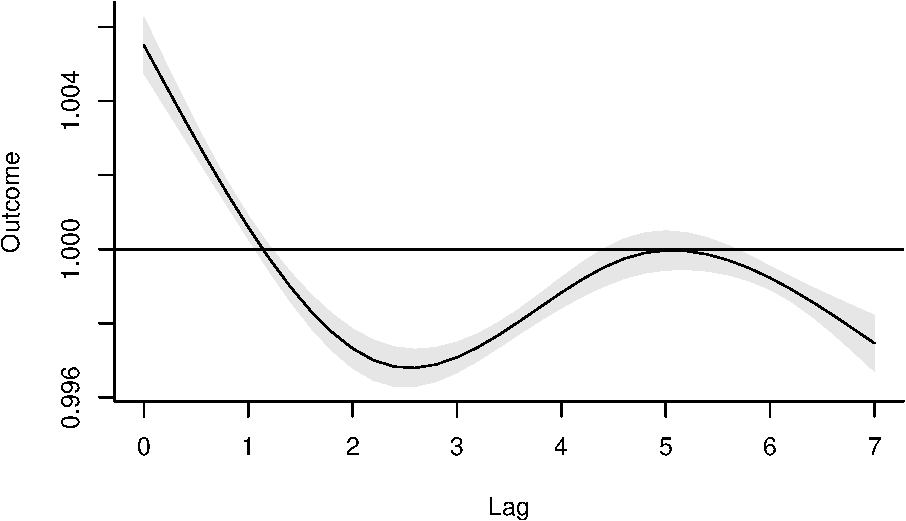
\includegraphics{adv_epi_analysis_files/figure-latex/unnamed-chunk-100-1.pdf}

You can go back to the \texttt{crossbasis} call and try playing around with the degrees of freedom
for the spline, to see how that affects the shape of this function. Be sure, though, that
you don't use more degrees of freedom than there are lags (i.e., more than 8).

Now let's try to extend the model out to look at up to a month after exposure. To do this,
all you need to do is change the \texttt{lag} argument in \texttt{crossbasis} to the longest lag you
want to include. Since we're adding more lags, you'll likely also want to increase the
degrees of freedom you use for the basis function of lag; here, I'm using 6, but you can
explore other values as well (again, don't use more than the number of lags, though).
From there, the process of fitting the model and plotting the results is identical.

\begin{Shaded}
\begin{Highlighting}[]
\NormalTok{dl\_basis\_3 }\OtherTok{\textless{}{-}} \FunctionTok{crossbasis}\NormalTok{(obs}\SpecialCharTok{$}\NormalTok{tmean, }\AttributeTok{lag =} \DecValTok{30}\NormalTok{,}
                       \AttributeTok{argvar =} \FunctionTok{list}\NormalTok{(}\AttributeTok{fun =} \StringTok{"lin"}\NormalTok{), }
                       \AttributeTok{arglag =} \FunctionTok{list}\NormalTok{(}\AttributeTok{fun =} \StringTok{"ns"}\NormalTok{, }\AttributeTok{df =} \DecValTok{6}\NormalTok{))}
\NormalTok{dist\_lag\_mod\_4 }\OtherTok{\textless{}{-}} \FunctionTok{glm}\NormalTok{(all }\SpecialCharTok{\textasciitilde{}}\NormalTok{ dl\_basis\_3 }\SpecialCharTok{+} 
                        \FunctionTok{factor}\NormalTok{(dow, }\AttributeTok{ordered =} \ConstantTok{FALSE}\NormalTok{) }\SpecialCharTok{+}
                          \FunctionTok{ns}\NormalTok{(time, }\AttributeTok{df =} \DecValTok{158}\NormalTok{), }
                        \AttributeTok{data =}\NormalTok{ obs, }\AttributeTok{family =} \StringTok{"quasipoisson"}\NormalTok{)}
\FunctionTok{crosspred}\NormalTok{(dl\_basis\_3, dist\_lag\_mod\_4, }\AttributeTok{at =} \DecValTok{1}\NormalTok{) }\SpecialCharTok{\%\textgreater{}\%} 
  \FunctionTok{plot}\NormalTok{(}\AttributeTok{ptype =} \StringTok{"slices"}\NormalTok{, }\AttributeTok{var =} \DecValTok{1}\NormalTok{)}
\end{Highlighting}
\end{Shaded}

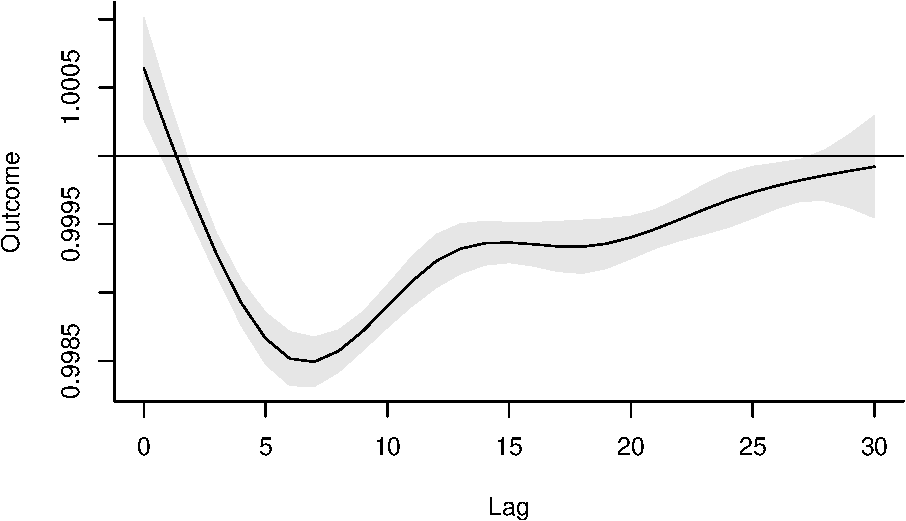
\includegraphics{adv_epi_analysis_files/figure-latex/unnamed-chunk-101-1.pdf}

\begin{enumerate}
\def\labelenumi{\arabic{enumi}.}
\setcounter{enumi}{2}
\tightlist
\item
  \textbf{Refine your model to fit for a non-linear, rather than linear, function
  of temperature, while also incorporating a function to describe lagged effects up
  to a month following exposure. Based on this model, what does the association
  between temperature and mortality look like at lag 0 days? How about at lag 21 days?
  What does the pattern of lagged effects look like when comparing the relative risk of
  mortality at a hot temperature (e.g., 28 degrees C) to a milder temperature
  (7 degrees C)? What about when comparing mortality at a cold temperature
  (e.g., -4 degrees C) to a milder temperature (7 degrees C)? If you use a constant
  term for the effect of exposure
  over a month as opposed to the smooth function you just used, how does the overall
  cumulative RR compare?}
\end{enumerate}

To extend the model to include temperature using a non-linear function, we'll go back
to the \texttt{crossbasis} call, but this time we'll make some changes to the exposure variable
dimension. The basis function for the exposure is set using the \texttt{argvar} (``var'' is
for ``variable'') parameter. Again, this allows us to include a list of parameters that
will be passed to \texttt{onebasis} to build a basis function and set up basis variables for
this dimension of the crossbasis. We can use a spline for temperature by specifying
\texttt{fun\ =\ "ns"}, as well as specify the degrees of freedom for that spline (here, I've used
4, but again, feel free to experiment):

\begin{Shaded}
\begin{Highlighting}[]
\NormalTok{dl\_basis\_4 }\OtherTok{\textless{}{-}} \FunctionTok{crossbasis}\NormalTok{(obs}\SpecialCharTok{$}\NormalTok{tmean, }\AttributeTok{lag =} \DecValTok{30}\NormalTok{,}
                       \AttributeTok{argvar =} \FunctionTok{list}\NormalTok{(}\AttributeTok{fun =} \StringTok{"ns"}\NormalTok{, }\AttributeTok{df =} \DecValTok{4}\NormalTok{), }
                       \AttributeTok{arglag =} \FunctionTok{list}\NormalTok{(}\AttributeTok{fun =} \StringTok{"ns"}\NormalTok{, }\AttributeTok{df =} \DecValTok{6}\NormalTok{))}
\end{Highlighting}
\end{Shaded}

Try looking at the crossbasis from this function (you'll need to look past the 30th row
or so, since the earliest rows will all be missing since they're in that range where
they don't have lag data available for the exposure). You can see that we now have a
\emph{lot} of columns: specifically, we have 4 (degrees of freedom for the temperature spline)
times 6 (degrees of freedom for the lag spline) = 24 columns.

\begin{Shaded}
\begin{Highlighting}[]
\NormalTok{dl\_basis\_4 }\SpecialCharTok{\%\textgreater{}\%} 
  \FunctionTok{as.data.frame}\NormalTok{() }\SpecialCharTok{\%\textgreater{}\%} 
  \FunctionTok{slice}\NormalTok{(}\DecValTok{28}\SpecialCharTok{:}\DecValTok{38}\NormalTok{)}
\end{Highlighting}
\end{Shaded}

\begin{verbatim}
##       v1.l1    v1.l2    v1.l3    v1.l4    v1.l5       v1.l6      v2.l1
## 1        NA       NA       NA       NA       NA          NA         NA
## 2        NA       NA       NA       NA       NA          NA         NA
## 3        NA       NA       NA       NA       NA          NA         NA
## 4  2.068939 3.299498 3.111270 1.738184 2.541810 -0.51512317 -0.5552531
## 5  1.955177 3.314862 3.125558 1.820183 2.690445 -0.40693744 -0.5967078
## 6  1.886111 3.299149 3.148516 1.893007 2.766242 -0.32385143 -0.6273517
## 7  1.882405 3.248469 3.180797 1.927784 2.804239 -0.08305771 -0.6419354
## 8  1.852973 3.165440 3.220817 1.900001 2.905860  0.08447527 -0.6588751
## 9  1.757370 3.058913 3.263914 1.795344 3.175517  0.03686863 -0.7106452
## 10 1.760596 2.944202 3.299498 1.779203 3.259667 -0.16712630 -0.7084665
## 11 1.797646 2.838520 3.314862 1.698607 3.497240 -0.17786583 -0.7118631
##         v2.l2      v2.l3      v2.l4      v2.l5         v2.l6    v3.l1    v3.l2
## 1          NA         NA         NA         NA            NA       NA       NA
## 2          NA         NA         NA         NA            NA       NA       NA
## 3          NA         NA         NA         NA            NA       NA       NA
## 4  -0.7011824 -0.7707934 -0.4847858 -0.9916438 -0.0956588789 1.405249 1.838701
## 5  -0.6979016 -0.7603742 -0.4547662 -0.9667940 -0.0791413415 1.478133 1.830775
## 6  -0.7047091 -0.7492423 -0.4287099 -0.9503322 -0.0554076103 1.526744 1.841501
## 7  -0.7234011 -0.7371123 -0.4081381 -0.9450033 -0.0058689802 1.541114 1.873929
## 8  -0.7537142 -0.7241504 -0.4035141 -0.9205842  0.0358717107 1.565836 1.927170
## 9  -0.7930344 -0.7111578 -0.4381402 -0.7997450 -0.0007806944 1.643309 1.996194
## 10 -0.8364025 -0.7011824 -0.4373333 -0.7657041 -0.0621066847 1.644968 2.071685
## 11 -0.8780716 -0.6979016 -0.4735973 -0.6384769 -0.0958995727 1.631672 2.143093
##       v3.l3    v3.l4    v3.l5       v3.l6      v4.l1     v4.l2     v4.l3
## 1        NA       NA       NA          NA         NA        NA        NA
## 2        NA       NA       NA          NA         NA        NA        NA
## 3        NA       NA       NA          NA         NA        NA        NA
## 4  1.955381 1.180876 2.353392  0.20605400 -0.8041945 -1.052250 -1.119024
## 5  1.942554 1.126503 2.294679  0.17194514 -0.8459049 -1.047714 -1.111683
## 6  1.926528 1.081359 2.257968  0.12135036 -0.8737239 -1.053852 -1.102512
## 7  1.906672 1.048474 2.249542  0.01133949 -0.8819473 -1.072411 -1.091149
## 8  1.883354 1.051489 2.198457 -0.07875894 -0.8960954 -1.102879 -1.077804
## 9  1.858659 1.116576 2.004017 -0.03652356 -0.9404317 -1.142380 -1.063672
## 10 1.838701 1.121782 1.943746  0.09297047 -0.9413808 -1.185582 -1.052250
## 11 1.830775 1.177720 1.763872  0.11448195 -0.9337721 -1.226447 -1.047714
##         v4.l4     v4.l5        v4.l6
## 1          NA        NA           NA
## 2          NA        NA           NA
## 3          NA        NA           NA
## 4  -0.6757908 -1.346797 -0.117920408
## 5  -0.6446743 -1.313197 -0.098400617
## 6  -0.6188389 -1.292188 -0.069446282
## 7  -0.6000200 -1.287366 -0.006489356
## 8  -0.6017453 -1.258131  0.045072099
## 9  -0.6389933 -1.146857  0.020901671
## 10 -0.6419722 -1.112366 -0.053205061
## 11 -0.6739847 -1.009427 -0.065515636
\end{verbatim}

The \texttt{dlnm} package has done
the work of setting up this crossbasis function, as well as creating this matrix of
basis variables from our original simple column of temperature measurements. This
is getting to be a much more complex function than the simple linear/unconstrained lag
function that we started with. However, the underlying principles and mechanics are the
same, they're just scaling up to allow some more complex ``shapes'' in our exposure-response
association.

We can add this new crossbasis function to the regression model, and then predict from
the crossbasis and regression model to get a view of how temperature is (non-linearly) associated
with mortality risk at different lags, comparing to a baseline temperature of 7 degrees C:

\begin{Shaded}
\begin{Highlighting}[]
\NormalTok{dist\_lag\_mod\_5 }\OtherTok{\textless{}{-}} \FunctionTok{glm}\NormalTok{(all }\SpecialCharTok{\textasciitilde{}}\NormalTok{ dl\_basis\_4 }\SpecialCharTok{+} 
                        \FunctionTok{factor}\NormalTok{(dow, }\AttributeTok{ordered =} \ConstantTok{FALSE}\NormalTok{) }\SpecialCharTok{+}
                          \FunctionTok{ns}\NormalTok{(time, }\AttributeTok{df =} \DecValTok{158}\NormalTok{), }
                        \AttributeTok{data =}\NormalTok{ obs, }\AttributeTok{family =} \StringTok{"quasipoisson"}\NormalTok{)}

\NormalTok{cp\_dl }\OtherTok{\textless{}{-}} \FunctionTok{crosspred}\NormalTok{(dl\_basis\_4, dist\_lag\_mod\_5, }\AttributeTok{cen =} \DecValTok{7}\NormalTok{, }\AttributeTok{bylag =} \DecValTok{1}\NormalTok{)}
\end{Highlighting}
\end{Shaded}

The object created by \texttt{crosspred} includes a \emph{lot} of output (you can check out the
whole thing by running \texttt{cp\_dl} to print it out). We can extract elements from this object
(for example, if we want to get effect estimates or estimates of confidence intervals).
We can also create a variety of plots from this object. The following plots all use the
\texttt{plot} method for \texttt{crosspred} objects, so you can access the helpfile with \texttt{?plot.crosspred}.

First, we can look at ``slices,'' where we focus on just one lag value and look at the non-linear relationship between temperature and mortality risk at that lag only. For example, here are plots showing the relationship between temperature and mortality risk on the same day of exposure (lag 0) and 21 days after exposure (lag 21):

\begin{Shaded}
\begin{Highlighting}[]
\FunctionTok{plot}\NormalTok{(cp\_dl, }\AttributeTok{ptype =} \StringTok{"slices"}\NormalTok{, }\AttributeTok{lag =} \DecValTok{0}\NormalTok{)}
\end{Highlighting}
\end{Shaded}

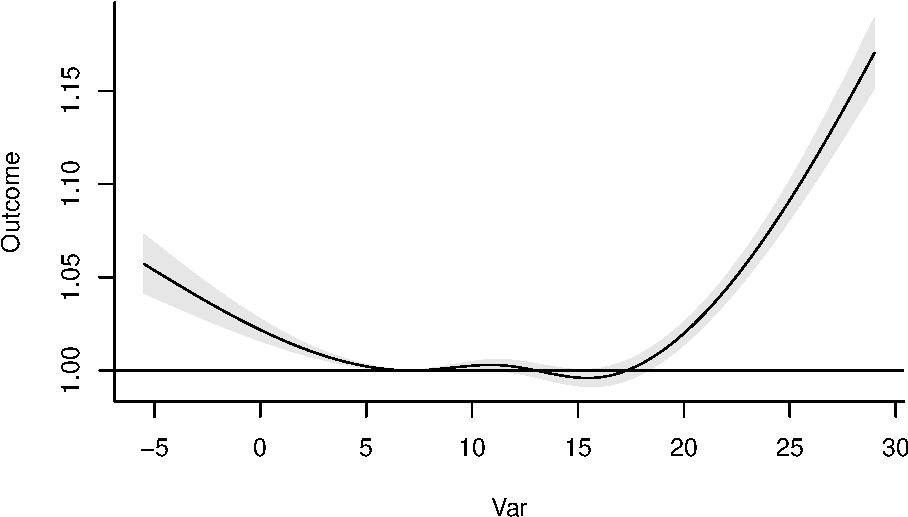
\includegraphics{adv_epi_analysis_files/figure-latex/unnamed-chunk-105-1.pdf}

\begin{Shaded}
\begin{Highlighting}[]
\FunctionTok{plot}\NormalTok{(cp\_dl, }\AttributeTok{ptype =} \StringTok{"slices"}\NormalTok{, }\AttributeTok{lag =} \DecValTok{21}\NormalTok{)}
\end{Highlighting}
\end{Shaded}

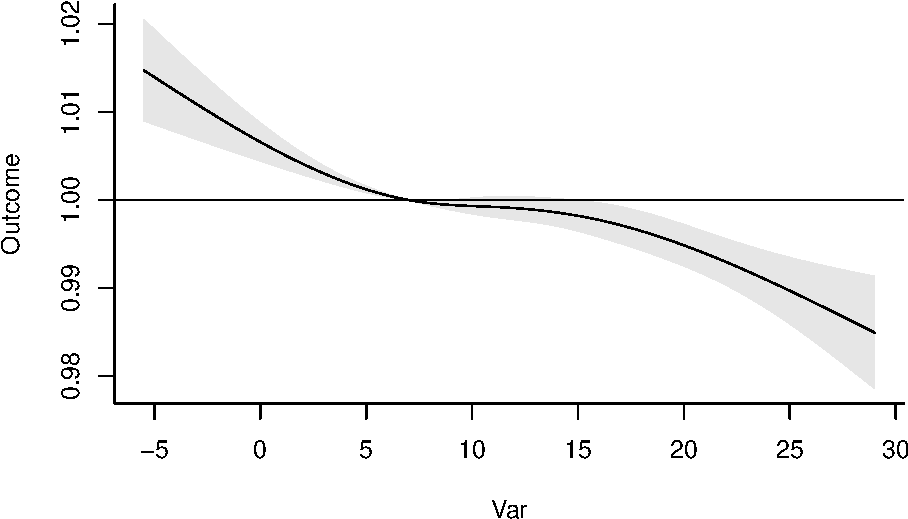
\includegraphics{adv_epi_analysis_files/figure-latex/unnamed-chunk-105-2.pdf}

You can see that heat has a stronger relationship with mortality risk than cold at lag 0,
while at a longer lag, there continues to be a positive association between cold temperature
and mortality risk, but now the relationship with heat has shifted to be negative.

You can do the same idea of looking at a ``slice'' for a specific temperature, in this case
seeing how effects vary across lags when comparing that temperature to the baseline temperature
(7 degrees C, which we set when we ran \texttt{crosspred}). For example, here are ``slices'' for
28 degrees C and -4 degrees C:

\begin{Shaded}
\begin{Highlighting}[]
\FunctionTok{plot}\NormalTok{(cp\_dl, }\AttributeTok{ptype =} \StringTok{"slices"}\NormalTok{, }\AttributeTok{var =} \DecValTok{28}\NormalTok{)}
\end{Highlighting}
\end{Shaded}

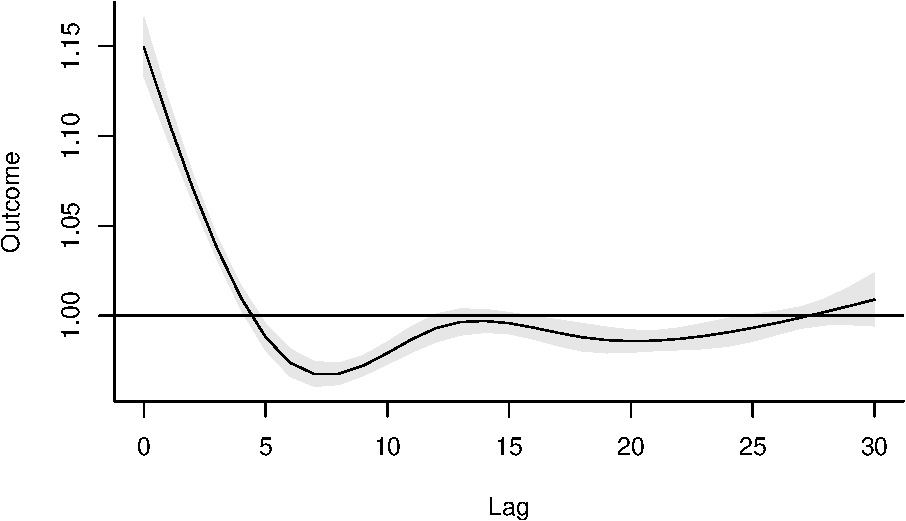
\includegraphics{adv_epi_analysis_files/figure-latex/unnamed-chunk-106-1.pdf}

\begin{Shaded}
\begin{Highlighting}[]
\FunctionTok{plot}\NormalTok{(cp\_dl, }\AttributeTok{ptype =} \StringTok{"slices"}\NormalTok{, }\AttributeTok{var =} \SpecialCharTok{{-}}\DecValTok{4}\NormalTok{)}
\end{Highlighting}
\end{Shaded}

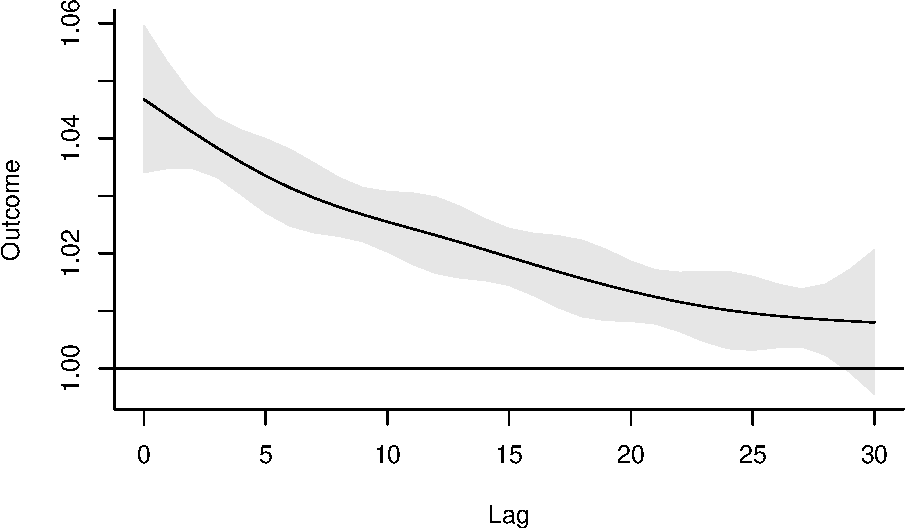
\includegraphics{adv_epi_analysis_files/figure-latex/unnamed-chunk-106-2.pdf}
These plots again reinforce that heat's association with mortality risk is more immediate,
while cold has an association that plays out over a much longer lag following exposure.

There are also some plots you can make from the \texttt{crosspred} object that help show the full,
three-dimensional association between the exposure, lag time, and risk of the outcome.
For example, the default plot created from the \texttt{crosspred} object is a three-dimensional
plot (the \texttt{theta}, \texttt{phi}, and \texttt{lphi} parameters shift the angle we view it from), while
the ``contour'' plot type shows us a contour plot of these results (in other words, showing
the exposure and lag variables in two dimensions of a two-dimensional plot then showing
relative risk using color for each combination). You can think of the `sliced' plots from above as two-dimensional slices of the three-dimensional graph if we slice right at the selected \texttt{lag} or \texttt{var} value. Here is the code to create those plots:

\begin{Shaded}
\begin{Highlighting}[]
\FunctionTok{plot}\NormalTok{(cp\_dl, }\AttributeTok{theta =} \DecValTok{200}\NormalTok{, }\AttributeTok{phi =} \DecValTok{40}\NormalTok{, }\AttributeTok{lphi =} \DecValTok{30}\NormalTok{)}
\end{Highlighting}
\end{Shaded}

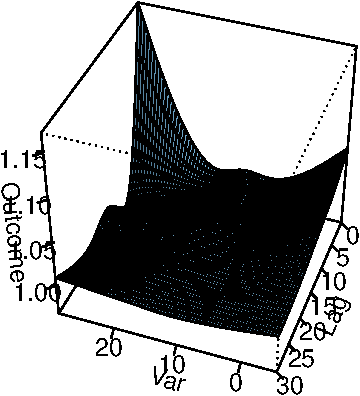
\includegraphics{adv_epi_analysis_files/figure-latex/unnamed-chunk-107-1.pdf}

\begin{Shaded}
\begin{Highlighting}[]
\FunctionTok{plot}\NormalTok{(cp\_dl, }\AttributeTok{ptype =} \StringTok{"contour"}\NormalTok{)}
\end{Highlighting}
\end{Shaded}

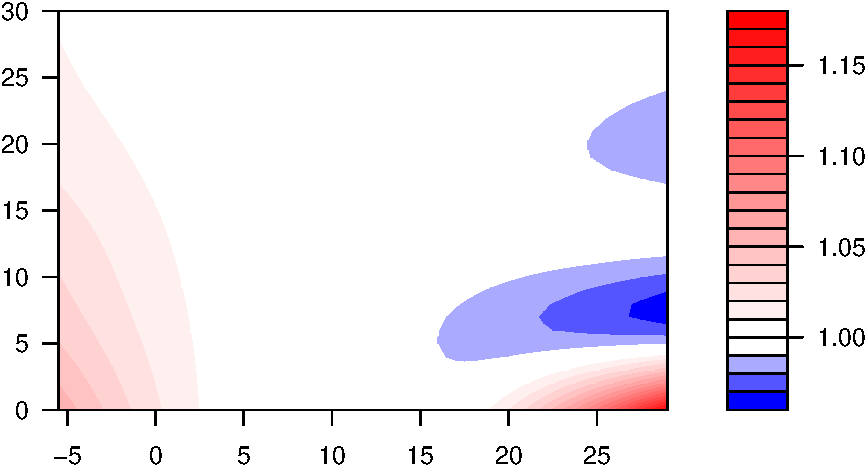
\includegraphics{adv_epi_analysis_files/figure-latex/unnamed-chunk-107-2.pdf}

To see how a `constant' lag-response model compares to the smooth function from this model we have to go back to the \texttt{crossbasis} and use the appropriate argument in the \texttt{arglag} parameter:

\begin{Shaded}
\begin{Highlighting}[]
\NormalTok{dl\_basis\_5 }\OtherTok{\textless{}{-}} \FunctionTok{crossbasis}\NormalTok{(obs}\SpecialCharTok{$}\NormalTok{tmean, }\AttributeTok{lag =} \DecValTok{30}\NormalTok{,}
                       \AttributeTok{argvar =} \FunctionTok{list}\NormalTok{(}\AttributeTok{fun =} \StringTok{"ns"}\NormalTok{, }\AttributeTok{df =} \DecValTok{4}\NormalTok{), }
                       \AttributeTok{arglag =} \FunctionTok{list}\NormalTok{(}\AttributeTok{fun =} \StringTok{"strata"}\NormalTok{, }\AttributeTok{df =} \DecValTok{1}\NormalTok{))}
\end{Highlighting}
\end{Shaded}

The function \texttt{strata} in \texttt{arglag} essentially breaks up the lag window into strata equaling the degrees of freedom specified, and the lag-response is assumed to be constant for each day within each stratum. Here we specified \texttt{df=1} so the lag-response is assumed to be constant for the entire lag window. In other words, the exposure in each day in the lag window is constrained to have the same effect. If we look at the \texttt{crossbasis} from this function you'll see that we have far fewer columns. Remember that the total number of columns is determined by the total number of degrees of freedom, which is the product of the df's in each of \texttt{argvar} and \texttt{arglag} so in this case 4.

\begin{Shaded}
\begin{Highlighting}[]
\NormalTok{dl\_basis\_5 }\SpecialCharTok{\%\textgreater{}\%} 
  \FunctionTok{as.data.frame}\NormalTok{() }\SpecialCharTok{\%\textgreater{}\%} 
  \FunctionTok{slice}\NormalTok{(}\DecValTok{28}\SpecialCharTok{:}\DecValTok{38}\NormalTok{)}
\end{Highlighting}
\end{Shaded}

\begin{verbatim}
##       v1.l1     v2.l1     v3.l1     v4.l1
## 1        NA        NA        NA        NA
## 2        NA        NA        NA        NA
## 3        NA        NA        NA        NA
## 4  14.69900 -4.438015 10.919532 -6.249020
## 5  15.03355 -4.382485 10.789984 -6.174883
## 6  15.21075 -4.347038 10.707109 -6.127455
## 7  15.33913 -4.332385 10.672850 -6.107850
## 8  15.51220 -4.298983 10.594759 -6.063160
## 9  15.89771 -4.127076 10.317738 -5.904626
## 10 15.96057 -4.094014 10.267995 -5.876159
## 11 16.37863 -3.880472  9.958228 -5.698886
\end{verbatim}

We can now run the same model as above replacing the \texttt{crossbasis} with the one we just created and
repeat the prediction to see how the temperature effect comparing to a baseline temperature
of 7 degrees C changes when we constrain the lag-response to be constant.

\begin{Shaded}
\begin{Highlighting}[]
\NormalTok{dist\_lag\_mod\_6 }\OtherTok{\textless{}{-}} \FunctionTok{glm}\NormalTok{(all }\SpecialCharTok{\textasciitilde{}}\NormalTok{ dl\_basis\_5 }\SpecialCharTok{+} 
                        \FunctionTok{factor}\NormalTok{(dow, }\AttributeTok{ordered =} \ConstantTok{FALSE}\NormalTok{) }\SpecialCharTok{+}
                          \FunctionTok{ns}\NormalTok{(time, }\AttributeTok{df =} \DecValTok{158}\NormalTok{), }
                        \AttributeTok{data =}\NormalTok{ obs, }\AttributeTok{family =} \StringTok{"quasipoisson"}\NormalTok{)}

\NormalTok{cp\_dlconstant }\OtherTok{\textless{}{-}} \FunctionTok{crosspred}\NormalTok{(dl\_basis\_5, dist\_lag\_mod\_6, }\AttributeTok{cen =} \DecValTok{7}\NormalTok{, }\AttributeTok{bylag =} \DecValTok{1}\NormalTok{)}
\end{Highlighting}
\end{Shaded}

If we look at the same plots and sliced plots as above we can see that this is a much simple model.

\begin{Shaded}
\begin{Highlighting}[]
\FunctionTok{plot}\NormalTok{(cp\_dlconstant, }\AttributeTok{ptype =} \StringTok{"slices"}\NormalTok{, }\AttributeTok{lag =} \DecValTok{0}\NormalTok{)}
\FunctionTok{plot}\NormalTok{(cp\_dlconstant, }\AttributeTok{ptype =} \StringTok{"slices"}\NormalTok{, }\AttributeTok{lag =} \DecValTok{21}\NormalTok{)}
\end{Highlighting}
\end{Shaded}

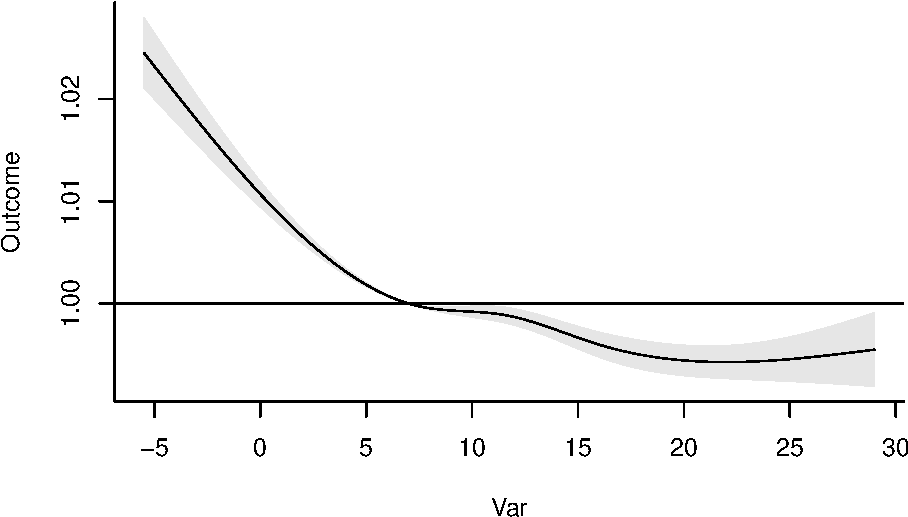
\includegraphics{adv_epi_analysis_files/figure-latex/unnamed-chunk-111-1.pdf}

The two plots are identical (because we assume that the exposure-response is the same at all lags) with colder temperatures having a negative effect, while the warmer temperatures appear to be protective.

\begin{Shaded}
\begin{Highlighting}[]
\FunctionTok{plot}\NormalTok{(cp\_dlconstant, }\AttributeTok{ptype =} \StringTok{"slices"}\NormalTok{, }\AttributeTok{var =} \DecValTok{28}\NormalTok{)}
\end{Highlighting}
\end{Shaded}

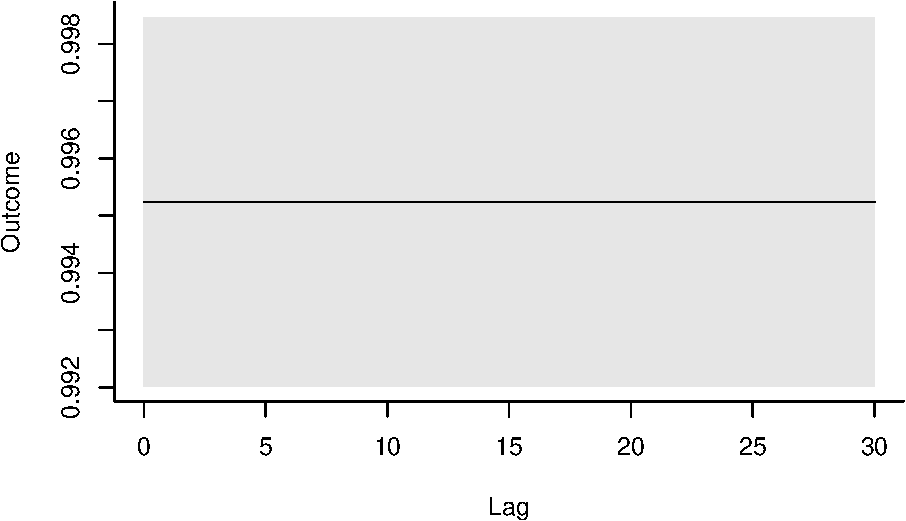
\includegraphics{adv_epi_analysis_files/figure-latex/unnamed-chunk-112-1.pdf}

\begin{Shaded}
\begin{Highlighting}[]
\FunctionTok{plot}\NormalTok{(cp\_dlconstant, }\AttributeTok{ptype =} \StringTok{"slices"}\NormalTok{, }\AttributeTok{var =} \SpecialCharTok{{-}}\DecValTok{4}\NormalTok{)}
\end{Highlighting}
\end{Shaded}

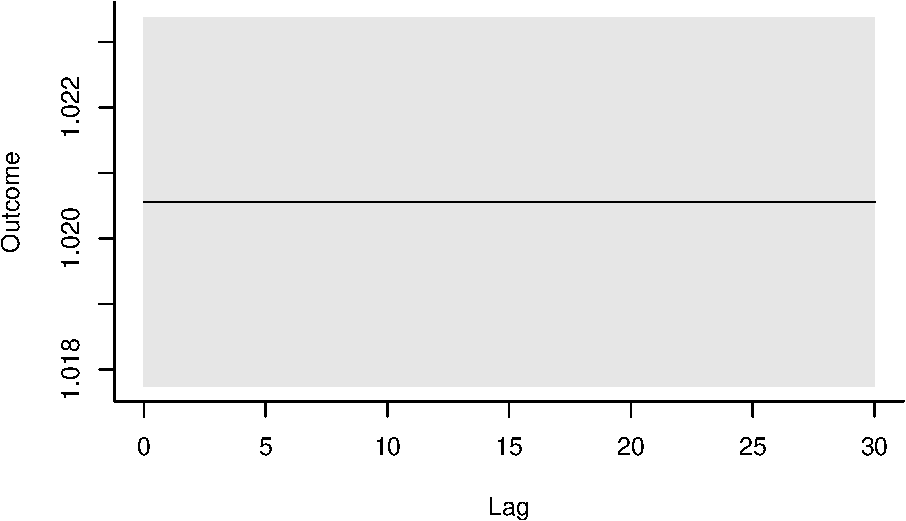
\includegraphics{adv_epi_analysis_files/figure-latex/unnamed-chunk-112-2.pdf}

Here we see the constant lag-response more clearly, but at different effects depending on the set temperature. The hot temperature appears to be mildly protective (RR \textless{} 1.0), while the cold temperature is harmful (RR \textgreater{} 1.0).

The reduced complexity is evident in the 3-d plot (which looks ``flat'' on one of the dimensions) and the contour plot (which has large rectangular areas) as well.

\begin{Shaded}
\begin{Highlighting}[]
\FunctionTok{plot}\NormalTok{(cp\_dlconstant, }\AttributeTok{theta =} \DecValTok{200}\NormalTok{, }\AttributeTok{phi =} \DecValTok{40}\NormalTok{, }\AttributeTok{lphi =} \DecValTok{30}\NormalTok{)}
\end{Highlighting}
\end{Shaded}

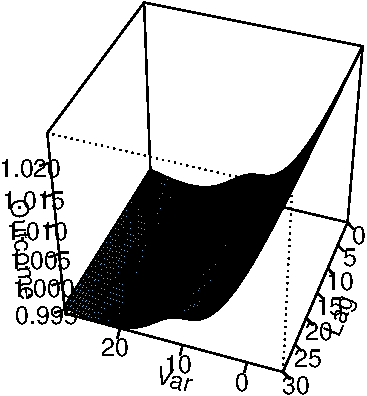
\includegraphics{adv_epi_analysis_files/figure-latex/unnamed-chunk-113-1.pdf}

\begin{Shaded}
\begin{Highlighting}[]
\FunctionTok{plot}\NormalTok{(cp\_dlconstant, }\AttributeTok{ptype =} \StringTok{"contour"}\NormalTok{)}
\end{Highlighting}
\end{Shaded}

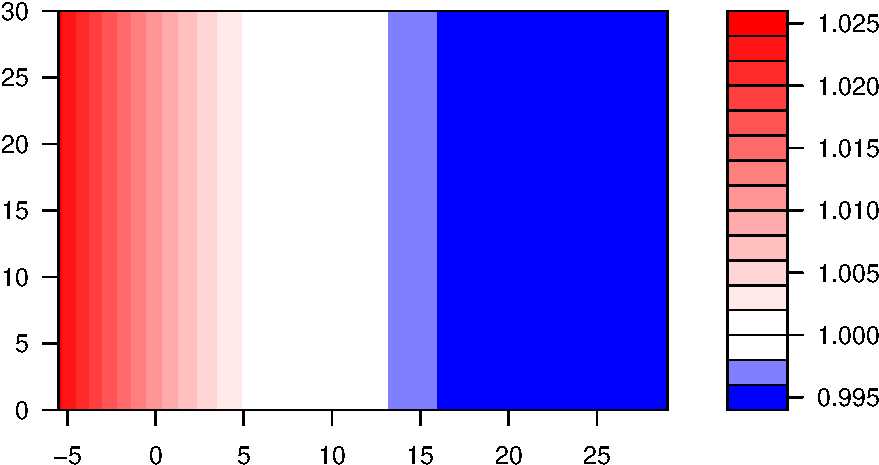
\includegraphics{adv_epi_analysis_files/figure-latex/unnamed-chunk-113-2.pdf}

One other thing that we can do with the model output is we can estimate the cumulative risk
across lags, for example for a month of hot temperature (28 degrees C) compared to cooler temperature (7 degrees C). We do this by essentially accumulating the RRs from each lag-day as follows. The crosspred object has estimates of the coefficients for each lag day (in the
\texttt{matfit} element), and you
could add these up yourself, or you can extract a difference element (\texttt{allfit}) that has
already added these up for you to get a cumulative effect estimate. If you'd like to
calculate confidence intervals, you can get an estimate of the standard error for this
cumulative estimate with the \texttt{allse} element of the crosspred object. We can get all these
for a temperature of 28 degrees C; since we set the crosspred object to be centered at
7 degrees C, this will allow us to compare 28 to 7 degrees C:

\begin{Shaded}
\begin{Highlighting}[]
\DocumentationTok{\#\#\# parameter for each lag{-}day}
\NormalTok{cp\_dlconstant}\SpecialCharTok{$}\NormalTok{matfit[cp\_dlconstant}\SpecialCharTok{$}\NormalTok{predvar}\SpecialCharTok{==}\DecValTok{28}\NormalTok{]}
\end{Highlighting}
\end{Shaded}

\begin{verbatim}
##  [1] -0.004774825 -0.004774825 -0.004774825 -0.004774825 -0.004774825
##  [6] -0.004774825 -0.004774825 -0.004774825 -0.004774825 -0.004774825
## [11] -0.004774825 -0.004774825 -0.004774825 -0.004774825 -0.004774825
## [16] -0.004774825 -0.004774825 -0.004774825 -0.004774825 -0.004774825
## [21] -0.004774825 -0.004774825 -0.004774825 -0.004774825 -0.004774825
## [26] -0.004774825 -0.004774825 -0.004774825 -0.004774825 -0.004774825
## [31] -0.004774825
\end{verbatim}

\begin{Shaded}
\begin{Highlighting}[]
\DocumentationTok{\#\#\# combined model parameter for the cumulative RR (this is the sum for all of the above parameters)}
\NormalTok{cp\_dlconstant}\SpecialCharTok{$}\NormalTok{allfit[cp\_dlconstant}\SpecialCharTok{$}\NormalTok{predvar}\SpecialCharTok{==}\DecValTok{28}\NormalTok{]}
\end{Highlighting}
\end{Shaded}

\begin{verbatim}
##         28 
## -0.1480196
\end{verbatim}

\begin{Shaded}
\begin{Highlighting}[]
\DocumentationTok{\#\#\# corresponding standard error for the cumulative RR parameter}
\NormalTok{cp\_dlconstant}\SpecialCharTok{$}\NormalTok{allse[cp\_dlconstant}\SpecialCharTok{$}\NormalTok{predvar}\SpecialCharTok{==}\DecValTok{28}\NormalTok{]}
\end{Highlighting}
\end{Shaded}

\begin{verbatim}
##         28 
## 0.05128501
\end{verbatim}

If we exponentiate the model parameter we will get the cumulative RR estimate and likewise using the model parameter and standard error we can derive 95\% Confidence Intervals (CIs) for the cumulative RR. For the central estimate:

\[
RR=exp(\beta)=exp(-0.148)=0.86
\]
For the confidence interval:

\[
exp(\beta \pm 1.96*se) = exp(-0.148 \pm 1.96*0.05) = (0.78, 0.95)
\]

The \texttt{crosspred} object, it turns out, stores this information as well (in the \texttt{allRRfit}, \texttt{allRRlow}, and \texttt{allRRhigh} elements), so we can extract these elements directly without doing the math:

\begin{Shaded}
\begin{Highlighting}[]
\NormalTok{cp\_dlconstant}\SpecialCharTok{$}\NormalTok{allRRfit[cp\_dlconstant}\SpecialCharTok{$}\NormalTok{predvar}\SpecialCharTok{==}\DecValTok{28}\NormalTok{]}
\end{Highlighting}
\end{Shaded}

\begin{verbatim}
##        28 
## 0.8624142
\end{verbatim}

\begin{Shaded}
\begin{Highlighting}[]
\NormalTok{cp\_dlconstant}\SpecialCharTok{$}\NormalTok{allRRlow[cp\_dlconstant}\SpecialCharTok{$}\NormalTok{predvar}\SpecialCharTok{==}\DecValTok{28}\NormalTok{]}
\end{Highlighting}
\end{Shaded}

\begin{verbatim}
##        28 
## 0.7799415
\end{verbatim}

\begin{Shaded}
\begin{Highlighting}[]
\NormalTok{cp\_dlconstant}\SpecialCharTok{$}\NormalTok{allRRhigh[cp\_dlconstant}\SpecialCharTok{$}\NormalTok{predvar}\SpecialCharTok{==}\DecValTok{28}\NormalTok{]}
\end{Highlighting}
\end{Shaded}

\begin{verbatim}
##        28 
## 0.9536078
\end{verbatim}

Does this look accurate? Do we expect a 14\% decrease in mortality comparing a very hot month to a cool month?

Now let's calculate the cumulative RR for temperature at 28 degrees for the smooth lag-response function model from before (i.e., pull those same elements from the model we fit before
with a smoother lag-response function):

\begin{Shaded}
\begin{Highlighting}[]
\NormalTok{cp\_dl}\SpecialCharTok{$}\NormalTok{allRRfit[cp\_dl}\SpecialCharTok{$}\NormalTok{predvar}\SpecialCharTok{==}\DecValTok{28}\NormalTok{]}
\end{Highlighting}
\end{Shaded}

\begin{verbatim}
##       28 
## 1.078548
\end{verbatim}

\begin{Shaded}
\begin{Highlighting}[]
\NormalTok{cp\_dl}\SpecialCharTok{$}\NormalTok{allRRlow[cp\_dl}\SpecialCharTok{$}\NormalTok{predvar}\SpecialCharTok{==}\DecValTok{28}\NormalTok{]}
\end{Highlighting}
\end{Shaded}

\begin{verbatim}
##        28 
## 0.9768645
\end{verbatim}

\begin{Shaded}
\begin{Highlighting}[]
\NormalTok{cp\_dl}\SpecialCharTok{$}\NormalTok{allRRhigh[cp\_dl}\SpecialCharTok{$}\NormalTok{predvar}\SpecialCharTok{==}\DecValTok{28}\NormalTok{]}
\end{Highlighting}
\end{Shaded}

\begin{verbatim}
##       28 
## 1.190816
\end{verbatim}

Based on this model, we infer there's about a 6\% cumulative increase associated with a
temperature of 28 degrees C compared to 7 degrees.

Does this look more accurate? Which of the two lag-response functions is more likely to be true?

\begin{enumerate}
\def\labelenumi{\arabic{enumi}.}
\setcounter{enumi}{3}
\tightlist
\item
  \textbf{Assume that we are interested in the potential effect of a 5-day
  heatwave occurring on lags 0 to 4? You can assess this as the effect of hot temperature
  (e.g., 28 degrees C) during these lags, while the temperature remains warm but more
  mild (e.g., 20 degrees C) the rest of the month, against constant 20 degrees C for
  the whole month. What is the effect under the `constant' model? How about the smooth
  function lag model?}
\end{enumerate}

Using the \texttt{crosspred} function we can compare any exposure history over a lag-window of interest to a reference value (or values varying over time in the same window). Realistically, a whole month of extremely high exposures is unlikely. Extreme phenomena (such as 28 degree mean daily temperature in London) are more likely to last a shorter period of time. Furthermore, the effect of an event like a heat wave (likely occurring in the summer) is probably better assessed with a referent value more akin to what the heat wave is replacing, i.e., a warm but more mild summer temperature rather than temperatures more likely to occur in other seasons. We saw above that the effect of hot temperatures tends to be more short term, so let's assess the potential effect of a 5-day heatwave assessed on the last day of the heatwave. The rest of the days in the month are at 20 degrees C and we will use the same value as the referent value for the whole month. Realistically there will be variability in the temperatures during these days as well, but for the purposes of this exercise let's keep it constant at 20 for simplicity. Let's assess this effect using the constant lag-response model.

\begin{Shaded}
\begin{Highlighting}[]
\NormalTok{hw\_constant }\OtherTok{\textless{}{-}} \FunctionTok{crosspred}\NormalTok{(dl\_basis\_5, dist\_lag\_mod\_6, }
                         \AttributeTok{at =} \FunctionTok{exphist}\NormalTok{(}\FunctionTok{c}\NormalTok{(}\FunctionTok{rep}\NormalTok{(}\DecValTok{20}\NormalTok{, }\DecValTok{26}\NormalTok{), }\FunctionTok{rep}\NormalTok{(}\DecValTok{28}\NormalTok{, }\DecValTok{5}\NormalTok{)), }\AttributeTok{times =} \DecValTok{31}\NormalTok{, }\AttributeTok{lag =} \DecValTok{30}\NormalTok{) , }
                         \AttributeTok{cen =} \DecValTok{20}\NormalTok{, }\AttributeTok{bylag =} \DecValTok{1}\NormalTok{)}
\end{Highlighting}
\end{Shaded}

The \texttt{exphist} function allows us to designate distinct exposure values for the entire lag-window. The exposure values here appear in an oldest (lag30) to most recent (lag0) order. The \texttt{times} argument determines were the list of exposure begins in the lag window (here \texttt{time\ =\ 31} or lag30 from 0-30). The effect estimate and corresponding CI can be extracted as above.

\begin{Shaded}
\begin{Highlighting}[]
\NormalTok{hw\_constant}\SpecialCharTok{$}\NormalTok{allRRfit}
\end{Highlighting}
\end{Shaded}

\begin{verbatim}
##       31 
## 1.004005
\end{verbatim}

\begin{Shaded}
\begin{Highlighting}[]
\NormalTok{hw\_constant}\SpecialCharTok{$}\NormalTok{allRRlow}
\end{Highlighting}
\end{Shaded}

\begin{verbatim}
##        31 
## 0.9891951
\end{verbatim}

\begin{Shaded}
\begin{Highlighting}[]
\NormalTok{hw\_constant}\SpecialCharTok{$}\NormalTok{allRRhigh}
\end{Highlighting}
\end{Shaded}

\begin{verbatim}
##       31 
## 1.019037
\end{verbatim}

Now, lets repeat this with the smooth function lag-response model:

\begin{Shaded}
\begin{Highlighting}[]
\NormalTok{hw\_smooth}\OtherTok{\textless{}{-}}\FunctionTok{crosspred}\NormalTok{(dl\_basis\_4, dist\_lag\_mod\_5, }
                     \AttributeTok{at =} \FunctionTok{exphist}\NormalTok{(}\FunctionTok{c}\NormalTok{(}\FunctionTok{rep}\NormalTok{(}\DecValTok{20}\NormalTok{, }\DecValTok{26}\NormalTok{), }\FunctionTok{rep}\NormalTok{(}\DecValTok{28}\NormalTok{, }\DecValTok{5}\NormalTok{)), }\AttributeTok{times =} \DecValTok{31}\NormalTok{, }\AttributeTok{lag =} \DecValTok{30}\NormalTok{) , }
                     \AttributeTok{cen =} \DecValTok{20}\NormalTok{, }\AttributeTok{bylag =} \DecValTok{1}\NormalTok{)}

\NormalTok{hw\_smooth}\SpecialCharTok{$}\NormalTok{allRRfit}
\end{Highlighting}
\end{Shaded}

\begin{verbatim}
##       31 
## 1.402728
\end{verbatim}

\begin{Shaded}
\begin{Highlighting}[]
\NormalTok{hw\_smooth}\SpecialCharTok{$}\NormalTok{allRRlow}
\end{Highlighting}
\end{Shaded}

\begin{verbatim}
##       31 
## 1.356389
\end{verbatim}

\begin{Shaded}
\begin{Highlighting}[]
\NormalTok{hw\_smooth}\SpecialCharTok{$}\NormalTok{allRRhigh}
\end{Highlighting}
\end{Shaded}

\begin{verbatim}
##       31 
## 1.450651
\end{verbatim}

We see that the constant lag-response model underestimates the RR and does not capture any potential effect of a heatwave, while the smooth term lag-response model indicates that there is a 40\% increase in mortality for the last day of the heatwave. Note that this increase in mortality is not the only effect, as based on out model the heatwave started having an effect on the same day it started, i.e.~we would expect all 5 heatwave days to have a temperature related increase in mortality compared to the days before the heat-wave. We can look at the increase in mortality for each day if we look at the individual effect estimates:

\begin{Shaded}
\begin{Highlighting}[]
\DocumentationTok{\#\#\# individual lag{-}day parameters}
\NormalTok{hw\_smooth}\SpecialCharTok{$}\NormalTok{matfit}
\end{Highlighting}
\end{Shaded}

\begin{verbatim}
##         lag0       lag1       lag2       lag3       lag4 lag5 lag6 lag7 lag8
## 31 0.1196662 0.09213574 0.06563143 0.04117951 0.01980617    0    0    0    0
##    lag9 lag10 lag11 lag12 lag13 lag14 lag15 lag16 lag17 lag18 lag19 lag20 lag21
## 31    0     0     0     0     0     0     0     0     0     0     0     0     0
##    lag22 lag23 lag24 lag25 lag26 lag27 lag28 lag29 lag30
## 31     0     0     0     0     0     0     0     0     0
\end{verbatim}

\begin{Shaded}
\begin{Highlighting}[]
\DocumentationTok{\#\#\#\# individual lag{-}day RRs}
\NormalTok{hw\_smooth}\SpecialCharTok{$}\NormalTok{matRRfit}
\end{Highlighting}
\end{Shaded}

\begin{verbatim}
##        lag0     lag1     lag2     lag3     lag4 lag5 lag6 lag7 lag8 lag9 lag10
## 31 1.127121 1.096514 1.067833 1.042039 1.020004    1    1    1    1    1     1
##    lag11 lag12 lag13 lag14 lag15 lag16 lag17 lag18 lag19 lag20 lag21 lag22
## 31     1     1     1     1     1     1     1     1     1     1     1     1
##    lag23 lag24 lag25 lag26 lag27 lag28 lag29 lag30
## 31     1     1     1     1     1     1     1     1
\end{verbatim}

The first day of the heatwave will have an effect corresponding to a lag0 effect:

\[
RR=exp(0.107)=1.11
\]

The second day of the heatwave will have an effect corresponding to a lag0 and lag1 effect:

\[
RR = exp(0.107 + 0.085) = 1.21
\]

(This quantity is also equal to the product of the lag-day specific RRs for lag0 and lag1:)

\[
1.11 \times 1.09 = 1.21
\]

And so on, until we reach our last day of the heatwave with RR=1.39. There is a bidirectional relationship for this RR, as you can interpret this as the overall effect of the heatwave on mortality on the last day of the heatwave, or as the overall effect of temperature on the first day of the heatwave on mortality over the next 5 days.

\chapter{Natural experiments}\label{natural-experiments}

\section{Readings}\label{readings-2}

The readings for this chapter are:

\begin{itemize}
\tightlist
\item
  \citet{bernal2017interrupted} (on interrupted time series), with a correction to an equation in the paper at \url{https://academic.oup.com/ije/article/49/4/1414/5900884}. Example data and R code for the paper are available \href{https://oup.silverchair-cdn.com/oup/backfile/Content_public/Journal/ije/49/4/10.1093_ije_dyaa118/1/dyaa118_supplementary_data.zip?Expires=1623897009&Signature=BzYQrBg60cMKHYeDU~OIZYIFuRgEIPwQsWMjzON0dB~fL8y-8x4xdGIJQBBPgDxBIoUIGnjmShVf1jlVqzloo3IldAdVC78TZ~~XseYdJ9c590QRAR6m7mH~VbPe-fCnQSnZF0z2Qw9PZcSGITZeNr4YXPVY-~gtpgBeZiN0MpgEVBLVT5fYhhQBGbp0vxl1bKdUfNtF71fdVJrglkhSG8-M24A07LmAr8jThx4MQmSAzKCxA4VZLRE6To8zC3-rJlxyWiqrSTFsVQM2SN4R6UuxYoRsILRcIAr2sUfqgmaSlxBiYAf71PdGSrnBcXX3l0l7yuAftX5PYTwMKTyxOA__&Key-Pair-Id=APKAIE5G5CRDK6RD3PGA}{to download} through a Supplemental Appendix. (Also, note that there is a correction of one of the statistical model equations in this paper, given at the same web address.)
\item
  \citet{bor2014regression} A systematic review of regression discontinuity designs in epidemiological research
\item
  \citet{lopez2013effect} An example of an epidemiological study that uses an interrupted time series study design. Includes a nice discussion of strengths and limitations of the study design.
\end{itemize}

The following are supplemental readings (i.e., not required, but may be of
interest) associated with the material in this chapter:

\begin{itemize}
\tightlist
\item
  \citet{barone2011effects} The scientific paper highlighted as an example in the tutorial from the required reading
\item
  \citet{sargent2004reduced} Another paper providing an example of an interrupted time series design to study the health impacts of a smoking ban
\item
  \citet{casey2018retirements} A paper that leverages difference-in-differences, also in the context of a natural experiment
\item
  \citet{mendola2018invited} An Invited Commentary on the previous reading
\item
  \citet{venkataramani2016regression} A good overview of regression discontinuity designs in health-related research
\item
  \citet{turner2021creating} Provides reccomendations on making graphs to illustrate interrupted time series data
\item
  \citet{linden2017challenges} An interesting analysis of challenges to validity when an interrupted time series study is conducted without controls (i.e., with a single group)
\item
  \citet{bottomley2019analysing} Introduces a more complex approach for interrupted time series, where a control is included to help control for trends with time
\item
  \citet{dimick2014methods} A short overview of the difference-in-differences design
\item
  \citet{howe2016gotta} An example of a study that uses difference-in-differences, in this case to study the role of Pokemon GO on physical activity
\item
  \citet{maciejewski2020regression} A short overview of the regression discontinuity design
\item
  \citet{haber2021covid} An overview of potential study designs for assessing COVID-19 policies, including interrupted time series and difference-in-differences
\end{itemize}

\section{Natural experiments}\label{natural-experiments-1}

If you want to test a scientific hypothesis---like whether a vaccine has a certain success rate in preventing infection---the ideal way to do it is to run a randomized controlled experiment. The ``controlled'' part of the experiment indicates that there will be some study subjects that get the treatment and some that instead will serve as a comparison by not being treated---that is, they will be controls. The randomized part of the experiment is that you will divide the study subjects into groups of treated and controls randomly, rather than through some method that could introduce confounding (like by assigning all study subjects in one city to treatment and all in other city to control).

The randomized controlled experiment is an extraordinary tool in science, as it allows a comparison of treated versus controls while in theory removing the risk of confounding by external factors. For an external factor to confound the estimate of an association, it must itself be associated with both the treatment (or exposure, in most cases for environmental epidemiology) and the outcome. By randomly distributing the study subjects into treatment or control, you (in theory) break any possibly association between external factors and the treatment. This ensures exchangeability between the treated and controls, and we can use one group as a proxy for the other. In other words the treated are a good indication of what would happen to the controls if they themselves were treated and the controls are a good inciation of what woud happn to the treated if they were assigned to be controls.

This is only ``in theory'' for a few reasons. First, unless you have huge numbers of study subjects, there is a reasonable chance that just by chance there will be some differences between treated and controlled groups in some external factors. For example, if you have ten study subjects, five female and five male, and you randomly distribute them into two groups, it wouldn't be that unusual to have one group with eight females and two males and the other with two females and eight males, and so there would remain an association between biological sex and treatment among the randomized study subjects. This chance is why you will often see, in papers describing randomized controlled experiments (e.g., for clinical trials), tables that give distributions of several external factors for the treatment and control groups. As you have more and more study subjects, it will become less likely to have a large difference in external factors by treatment group. One other reason, however, that the distribution of treatment is only random in theory is that some people may not comply or otherwise carry through with their assigned treatment. This mechanism is a risk regardless of the size of the study population. This could result from a subject not complying with the assigned treatment, but could also result from something like a doctor taking a study subject off the assigned treatment for one reason or another. We will revisit the issue of non-compliance, intention-to-treat analysis in a later chapter (instrumental variables).

Randomized controlled experiments are therefore powerful (although not ironclad). However, there are many cases in environmental epidemiology where we cannot use them. This is for both practical and ethical reasons. From a practical standpoint, for example, we may want to explore how tropical cyclones affect health risk. It is (currently) impossible to create a hurricane and ``apply'' it to a group of study subjects that you've assigned to be ``exposed''. From an ethical standpoint, many of the exposures we study in environmental epidemiology are harmful, and it can often be unethical to assign a study subject to an exposure that is known or thought to be harmful for the sake of science. (By contrast, in a clinical trial of a medication, there is a chance that the medication will have harmful side effects, but it's being tested because there is a chance it will improve the health of the study subjects.) There are some cases where randomized controlled experiments can be used in environmental epidemiology---for example, better designs of indoor cookstoves are hypothesized to improve health, and so could be tested in this way. However, for many research questions, environmental epidemiologists often rely on observational data to help answer the question, rather than data generated through a randomized controlled trial.

We have been using observational data in our examples up to this point, and we've explored how we can use a regression modeling framework to control for potential confounders. In other words, in these examples, since we were unable to use randomization of the treatment (i.e., exposure) to remove risk of confounding from external factors, we instead had to think very careful about which external factors might confound our estimate of the association and in what way, and then address those factors in the statistical modeling through the use of control variables and sensitivity analysis.

In this chapter, we'll look at another way that we can leverage observational data to test scientific hypotheses, and that's through natural experiments. To be clear, these two methods are not mutually exclusive; instead, you could build studies where you incorporate both a natural experiment as well as control for factors that might still cause some residual confounding if not controlled for.

A natural experiment occurs when something happens that divides a group of potential study subjects into some who are treated (or exposed) and some who are not, and does so in a way where this division should be pretty close to random, at least in regards to most external factors that could be confounders. This division could be by space---for example, you could have an exposure that hits one geographic area but spares a neighboring area that is otherwise very comparable. This division could also be by time---you could have a policy that is implemented at a certain date, and so the study population immediately before that date was unexposed to this new policy while those after the date were exposed.

Typically, the ``randomization'' of treatment (or exposure) imposed by the natural experiment won't be perfect, and it usually won't even be as good as what could be done under a controlled randomized experiment. However, it is often good enough that it allows us to use observational data, which is much easier and cheaper to get at a large scale than data generated by a controlled experiment. This has the advantages of increased statistical power, and in many cases observational data that cover a large scale may offer improved external validity for the study results, since the data are typically collected in conditions that more closely reflect ``real life'' conditions.

In this chapter, we will focus on a study design called an \emph{interrupted time series}. This study design can be applied in cases where there has been an abrupt change at a certain time point that would influence how treatment is assigned before and after that time point. For example, there might be a new law that prevents indoor smoking in restaurants. If that policy goes into effect on a specific date, then exposure to secondary smoke in the population would change abruptly to be lower (at least, on average across the population) after that date compared to before. As another example, if the workers at a factory that is a heavy polluter goes on strike (and so all equipment stops running) on a specific date, then the pollution exposure in that city might abruptly change from before the strike to during the strike, and then change again after the strike is over.

This study design belongs to a more general type of natural experiment study design called a ``regression discontinuity'' design. Broadly, a regression discontinuity design can be applied anytime there is a threshold at which the chance of treatment (or exposure) changes abruptly. Interrupted time series are limited to cases where this threshold comes at a specific time, and where you have collected time series data. However, there are plenty of set-ups that would create other regression discontinuities that could be exploited to answer a scientific hypothesis.

For example, some medications are prescribed based on a threshold. For example, a doctor might describe when to start drug treatment for HIV based on a certain threshold of white blood cells measured in the patient. In this case, the white blood cell count is negatively associated with disease severity and so with many outcomes from the disease, so you might expect many outcomes to increase in risk as this count decreases. However, if the treatment is helpful in decreasing risk for those outcomes, then it may be that people with white blood cell counts that are just barely low enough to receive treatment have lower risk of those outcomes than people just barely too high in the counts to receive treatment. The people just barely above the threshold are likely pretty similar to those just barely below the threshold, and so a ``discontinuity'' in the risk of health outcomes that happens as you cross that threshold is likely caused by the treatment, which changes abruptly while other factors change minimally if at all. In the next section of this chapter, we will explore how you can use a GLM regression model in the context of interrupted time series (and by extension, for regression discontinuity study designs in general).

\section{Interrupted time series}\label{interrupted-time-series}

In this section, we'll take a closer look at interrupted time series study designs, focusing on how you can use statistical models to fit time series data and draw conclusions from these studies.

First, for these studies, we will think about exposure in a slightly different way. In these studies, we often will not directly have the exposure that we care about. For example, the data in \citet{bernal2017interrupted} aims to improve knowledge of whether exposure to secondary smoke alters the acute risk of cardiovascular events. However, they do not have measures of secondary smoke exposure for all their study subjects. Instead, they know the date when a ban was introduced in the study location that banned indoor smoking in public places. We can assume that, on the date of this ban, people in this community had an abrupt reduction in their exposure to indoor secondary smoke.

As a reminder, interrupted time series designs are part of a more general group of designs, those for regression discontinuities. This general group of designs shares the characteristic that the exposure of interest is often not directly measured, but instead another factor is measured that, at a certain threshold, abruptly changes average exposure to the exposure we do care about. The changing factor (time in the case of an interrupted time series, white blood cell counts in the example given earlier on HIV treatment) is called the \emph{forcing variable} in the study, and the point along this variable at which the exposure of interest abruptly changes is called the \emph{threshold} or \emph{threshold rule} (\citep{bor2014regression} has a great overview of regression discontinuity studies in epidemiology with examples of different possible forcing variables and threshold rules).

\emph{Applied: Fitting a statistical regression model for data from an interrupted time series study}

We will use a new example dataset for this chapter---the dataset that comes with one of the required reading papers for this chapter, \citet{bernal2017interrupted}. Make sure you download the file named ``sicily.csv'' that comes as a supplement to this paper.

\begin{enumerate}
\def\labelenumi{\arabic{enumi}.}
\tightlist
\item
  Load the data into R and explore the dataset. Plot the time series of the data on the outcome of interest as it varies over the study period. Use a visual marker in the plot to show the intervention (the date the law was implemented).
\item
  Next, let's look at how the rates of the outcome changes right before and right after the ban. At this stage, we won't worry about any underlying time trends in the outcome rates. Instead, compare the outcome rates in two groups---the data points collected for the time points right before the ban, and then the data collected for time points right after the ban. Try a few windows for capturing ``right before'' and ``right after'' (e.g., 3 months, 6 months, 12 months). How does the precision of the estimate change as you change that window? How do you think the potential might change for residual confounding from long-term trends in the outcome rates irrespective of the ban?
\item
  Now see if you can fit a regression model that uses all the data, while using a regression term to allow for a long-term trend in the rates of the outcome. You may want to try out several of the model structures shown in Figure 2 of \citet{bernal2017interrupted}. Can you interpret the model coefficients that you get from fitting these models? What conclusions do you draw about whether rates of hospitalization for acute coronary events are affected by exposure to secondary smoke?
\item
  Now let's try to control for long-term and seasonal trends beyond the linear term for time. Fit a model using a harmonic term like in \citet{bernal2017interrupted}. Do the coefficients from the model for the smoking ban and linear time term change? In previous examples, we've been using flexible functions for this such as splines. Repeat the model from above using a spline term. How does this model compare with respect to the smoking ban coefficient? Why?
\end{enumerate}

\emph{Applied exercise: Example code}

\begin{enumerate}
\def\labelenumi{\arabic{enumi}.}
\tightlist
\item
  \textbf{Load the data into R and explore the dataset. Plot the time series of the data on the outcome of interest as it varies over the study period. Use a visual marker in the plot to show the intervention (the date the law was implemented).}
\end{enumerate}

These data are available in the paper's supplement. If you download the supplemental data file on the paper's website, it gives you a zipped file that you can unzip to create a directory of several files. This directory includes ``data/sicily.csv''. You'll need to move that to your working directory or a subdirectory of your working directory. In the code below, I have it in a subdirectory named ``data'' of my working directory. The data is in a plain text, comma-separated file (you can tell by the ``.csv'' file extension), so you can use \texttt{read\_csv} from the \texttt{tidyverse} suite of packages to read it in.

\begin{Shaded}
\begin{Highlighting}[]
\CommentTok{\# Load some packages that will likely be useful}
\FunctionTok{library}\NormalTok{(tidyverse)}
\FunctionTok{library}\NormalTok{(viridis)}
\FunctionTok{library}\NormalTok{(lubridate)}
\FunctionTok{library}\NormalTok{(broom)}

\CommentTok{\# Load and clean the data}
\NormalTok{sicily }\OtherTok{\textless{}{-}} \FunctionTok{read\_csv}\NormalTok{(}\StringTok{"data/sicily.csv"}\NormalTok{)}
\end{Highlighting}
\end{Shaded}

Once you read the data in, you should check it out:

\begin{Shaded}
\begin{Highlighting}[]
\NormalTok{sicily}
\end{Highlighting}
\end{Shaded}

\begin{verbatim}
## # A tibble: 59 x 7
##     year month  aces  time smokban     pop  stdpop
##    <dbl> <dbl> <dbl> <dbl>   <dbl>   <dbl>   <dbl>
##  1  2002     1   728     1       0 364277. 379875.
##  2  2002     2   659     2       0 364277. 376496.
##  3  2002     3   791     3       0 364277. 377041.
##  4  2002     4   734     4       0 364277. 377116.
##  5  2002     5   757     5       0 364277. 377383.
##  6  2002     6   726     6       0 364277. 374113.
##  7  2002     7   760     7       0 364277. 379513.
##  8  2002     8   740     8       0 364277. 376296.
##  9  2002     9   720     9       0 364277. 374653.
## 10  2002    10   814    10       0 364277. 378486.
## # i 49 more rows
\end{verbatim}

In this case, it looks like the time-step for observations is by month. In other words, we have one measurement per month. The \texttt{time} variable has already been added---this gives us the month in the study period. The outcome variable of interest is \texttt{aces}, which gives the number of hospital admissions for acute coronary events (ACEs) in each month.

The forcing variable in the study is, since it is an interrupted time series, \texttt{time}. We will be comparing risk of ACE hospitalizations before and after the date of the indoor smoking ban, so that date will form our threshold rule for the study. The creators of this dataset already added a variable with data on this threshold rule: the \texttt{smokban} variable is \texttt{0} before the ban and \texttt{1} after.

We can take a look using \texttt{smokban} to see when the ban was implemented. One
way to do this is to group the data by the \texttt{smokban} variable and then use \texttt{slice} to see the first three rows within each group. Based on this, it looks like the ban started the 37th month of the study:

\begin{Shaded}
\begin{Highlighting}[]
\NormalTok{sicily }\SpecialCharTok{\%\textgreater{}\%}  
  \FunctionTok{group\_by}\NormalTok{(smokban) }\SpecialCharTok{\%\textgreater{}\%} 
  \FunctionTok{slice}\NormalTok{(}\DecValTok{1}\SpecialCharTok{:}\DecValTok{3}\NormalTok{)}
\end{Highlighting}
\end{Shaded}

\begin{verbatim}
## # A tibble: 6 x 7
## # Groups:   smokban [2]
##    year month  aces  time smokban     pop  stdpop
##   <dbl> <dbl> <dbl> <dbl>   <dbl>   <dbl>   <dbl>
## 1  2002     1   728     1       0 364277. 379875.
## 2  2002     2   659     2       0 364277. 376496.
## 3  2002     3   791     3       0 364277. 377041.
## 4  2005     1   831    37       1 364421. 388153.
## 5  2005     2   796    38       1 364421. 388373.
## 6  2005     3   833    39       1 364421. 386470.
\end{verbatim}

Let's use a plot to explore the relationship between the forcing value (time) and the outcome (ACE hospitalizations) before we look at the remaining variables in the data.

\begin{Shaded}
\begin{Highlighting}[]
\FunctionTok{ggplot}\NormalTok{() }\SpecialCharTok{+} 
  \FunctionTok{geom\_polygon}\NormalTok{(}\FunctionTok{aes}\NormalTok{(}\AttributeTok{x =} \FunctionTok{c}\NormalTok{(}\DecValTok{37}\NormalTok{, }\DecValTok{59}\NormalTok{, }\DecValTok{59}\NormalTok{, }\DecValTok{37}\NormalTok{), }
                   \AttributeTok{y =} \FunctionTok{c}\NormalTok{(}\ConstantTok{Inf}\NormalTok{, }\ConstantTok{Inf}\NormalTok{, }\SpecialCharTok{{-}}\ConstantTok{Inf}\NormalTok{, }\SpecialCharTok{{-}}\ConstantTok{Inf}\NormalTok{)), }
               \AttributeTok{fill =} \StringTok{"cyan"}\NormalTok{, }\AttributeTok{alpha =} \FloatTok{0.2}\NormalTok{) }\SpecialCharTok{+} 
  \FunctionTok{geom\_point}\NormalTok{(}\AttributeTok{data =}\NormalTok{ sicily, }\FunctionTok{aes}\NormalTok{(}\AttributeTok{x =}\NormalTok{ time, }\AttributeTok{y =}\NormalTok{ aces)) }\SpecialCharTok{+} 
  \FunctionTok{labs}\NormalTok{(}\AttributeTok{x =} \StringTok{"Month in study"}\NormalTok{, }
       \AttributeTok{y =} \StringTok{"Number of hospitalizations}\SpecialCharTok{\textbackslash{}n}\StringTok{for acute coronary events"}\NormalTok{)}
\end{Highlighting}
\end{Shaded}

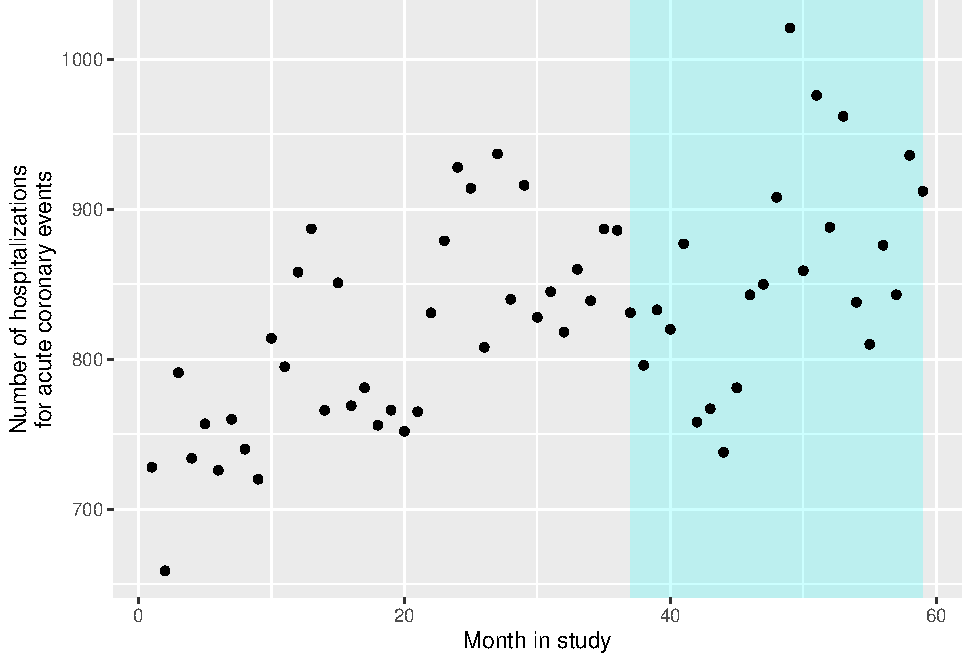
\includegraphics{adv_epi_analysis_files/figure-latex/unnamed-chunk-124-1.pdf}

As a note, to get this to work with \texttt{ggplot}, you need to be careful about where you specify the data. We've added the polygon using exact x and y values, rather than pulling them from a column in the dataframe (we knew from checking the data that the ban started for week 37 and then lasted the rest of the study, and there are 59 weeks in the study). Since we are only using the \texttt{sicily} data when we add points, but not when we add the polygon, we need to specify those data only for the the \texttt{geom\_point} layer, and not within \texttt{ggplot}. Also, the order of our layers matters a bit more here than it normally does. If we want the shaded polygon to go behind the points, we should add \texttt{geom\_polygon} before we add \texttt{geom\_point}, so the points get plotted on top.

Two other variables are also included in the data, \texttt{pop} and \texttt{stdpop}. These give measures of the study's population size for every time point in the study, as well as that population as an age-standardized population (in person-years). In our examples in earlier studies, we didn't incorporate the size of the study population in any way. We used counts of deaths, fitting them with a Poisson regression. If the size of the total population only changes slowly (in comparison to the time-scale of the association we were looking at, which was from days up to about a month), and if the disease outcome is rare (that is, unlikely on any study day for any population member), then it is typically fine not to include information about the total population size on each study day (or month, if that is your time step, as in the example for this study).

However, in some cases you will have a population that changes more abruptly. For example, if you may want to count outcomes based on insurance claims. If the number of enrollees for that insurance change substantially on certain dates (e.g., the start of the month or start of the year, which can be points where many new people become eligible for the insurance), you can get abrupt changes in the size of your study population.

If you have the population size for each observation in the time series, then you can address this when you fit your statistical model. You can still fit the data with a Poisson regression model, but you will include something called an \emph{offset}. You will include that in you regression model equation when you fit the regression with R, as we'll look at in the next part of the exercise. The \emph{offset} also allows us to model rates rather than counts as we show later in the chapter.

For right now, we can use the information about population size to change our plot a bit, so that it shows the rate of hospitalizations for coronary events (times 10,000) in each month of the study, rather than the unadjusted count:

\begin{Shaded}
\begin{Highlighting}[]
\FunctionTok{ggplot}\NormalTok{() }\SpecialCharTok{+} 
  \FunctionTok{geom\_polygon}\NormalTok{(}\FunctionTok{aes}\NormalTok{(}\AttributeTok{x =} \FunctionTok{c}\NormalTok{(}\DecValTok{37}\NormalTok{, }\DecValTok{59}\NormalTok{, }\DecValTok{59}\NormalTok{, }\DecValTok{37}\NormalTok{), }
                   \AttributeTok{y =} \FunctionTok{c}\NormalTok{(}\ConstantTok{Inf}\NormalTok{, }\ConstantTok{Inf}\NormalTok{, }\SpecialCharTok{{-}}\ConstantTok{Inf}\NormalTok{, }\SpecialCharTok{{-}}\ConstantTok{Inf}\NormalTok{)), }
               \AttributeTok{fill =} \StringTok{"cyan"}\NormalTok{, }\AttributeTok{alpha =} \FloatTok{0.2}\NormalTok{) }\SpecialCharTok{+} 
  \FunctionTok{geom\_point}\NormalTok{(}\AttributeTok{data =}\NormalTok{ sicily, }\FunctionTok{aes}\NormalTok{(}\AttributeTok{x =}\NormalTok{ time, }\AttributeTok{y =}\NormalTok{ aces }\SpecialCharTok{/}\NormalTok{ stdpop }\SpecialCharTok{*}\NormalTok{ (}\DecValTok{10} \SpecialCharTok{\^{}} \DecValTok{5}\NormalTok{))) }\SpecialCharTok{+} 
  \FunctionTok{labs}\NormalTok{(}\AttributeTok{x =} \StringTok{"Month in study"}\NormalTok{, }
       \AttributeTok{y =} \StringTok{"Number of hospitalizations}\SpecialCharTok{\textbackslash{}n}\StringTok{for acute coronary events * 10,000"}\NormalTok{)}
\end{Highlighting}
\end{Shaded}

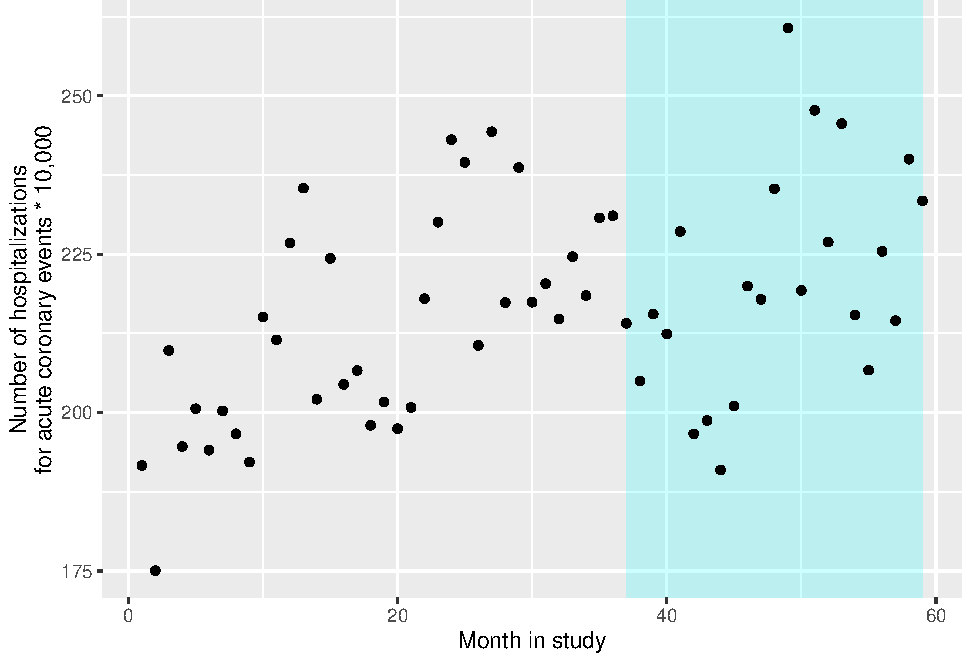
\includegraphics{adv_epi_analysis_files/figure-latex/unnamed-chunk-125-1.pdf}

\begin{enumerate}
\def\labelenumi{\arabic{enumi}.}
\setcounter{enumi}{1}
\tightlist
\item
  \textbf{Next, let's look at how the rates of the outcome changes right before and right after the ban. At this stage, we won't worry about any underlying time trends in the outcome rates. Instead, compare the outcome rates in two groups---the data points collected for the time points right before the ban, and then the data collected for time points right after the ban. Try a few windows for capturing ``right before'' and ``right after'' (e.g., 3 months, 6 months, 12 months). How does the precision of the estimate change as you change that window? How do you think the potential might change for residual confounding from long-term trends in the outcome rates irrespective of the ban?}
\end{enumerate}

Let's start with the smallest window, 3 months. This means that we will pick out
only the three data points before the ban (months 34, 35, and 36 of the study) and the three after (months 37, 38, and 39):

\begin{Shaded}
\begin{Highlighting}[]
\NormalTok{near\_threshold }\OtherTok{\textless{}{-}}\NormalTok{ sicily }\SpecialCharTok{\%\textgreater{}\%} 
  \FunctionTok{filter}\NormalTok{(time }\SpecialCharTok{\%in\%} \DecValTok{34}\SpecialCharTok{:}\DecValTok{39}\NormalTok{)}
\NormalTok{near\_threshold}
\end{Highlighting}
\end{Shaded}

\begin{verbatim}
## # A tibble: 6 x 7
##    year month  aces  time smokban     pop  stdpop
##   <dbl> <dbl> <dbl> <dbl>   <dbl>   <dbl>   <dbl>
## 1  2004    10   839    34       0 364700. 384052.
## 2  2004    11   887    35       0 364700. 384450.
## 3  2004    12   886    36       0 364700. 383428.
## 4  2005     1   831    37       1 364421. 388153.
## 5  2005     2   796    38       1 364421. 388373.
## 6  2005     3   833    39       1 364421. 386470.
\end{verbatim}

To check that we've pulled the right months, we can add these in a different color to our plot from the last section:

\begin{Shaded}
\begin{Highlighting}[]
\FunctionTok{ggplot}\NormalTok{() }\SpecialCharTok{+} 
  \FunctionTok{geom\_polygon}\NormalTok{(}\FunctionTok{aes}\NormalTok{(}\AttributeTok{x =} \FunctionTok{c}\NormalTok{(}\DecValTok{37}\NormalTok{, }\DecValTok{59}\NormalTok{, }\DecValTok{59}\NormalTok{, }\DecValTok{37}\NormalTok{), }
                   \AttributeTok{y =} \FunctionTok{c}\NormalTok{(}\ConstantTok{Inf}\NormalTok{, }\ConstantTok{Inf}\NormalTok{, }\SpecialCharTok{{-}}\ConstantTok{Inf}\NormalTok{, }\SpecialCharTok{{-}}\ConstantTok{Inf}\NormalTok{)), }
               \AttributeTok{fill =} \StringTok{"cyan"}\NormalTok{, }\AttributeTok{alpha =} \FloatTok{0.2}\NormalTok{) }\SpecialCharTok{+} 
  \FunctionTok{geom\_point}\NormalTok{(}\AttributeTok{data =}\NormalTok{ sicily, }\FunctionTok{aes}\NormalTok{(}\AttributeTok{x =}\NormalTok{ time, }\AttributeTok{y =}\NormalTok{ aces }\SpecialCharTok{/}\NormalTok{ stdpop }\SpecialCharTok{*}\NormalTok{ (}\DecValTok{10} \SpecialCharTok{\^{}} \DecValTok{5}\NormalTok{))) }\SpecialCharTok{+} 
  \FunctionTok{geom\_point}\NormalTok{(}\AttributeTok{data =}\NormalTok{ near\_threshold, }
             \FunctionTok{aes}\NormalTok{(}\AttributeTok{x =}\NormalTok{ time, }\AttributeTok{y =}\NormalTok{ aces }\SpecialCharTok{/}\NormalTok{ stdpop }\SpecialCharTok{*}\NormalTok{ (}\DecValTok{10} \SpecialCharTok{\^{}} \DecValTok{5}\NormalTok{)), }
             \AttributeTok{color =} \StringTok{"red"}\NormalTok{) }\SpecialCharTok{+} 
  \FunctionTok{labs}\NormalTok{(}\AttributeTok{x =} \StringTok{"Month in study"}\NormalTok{, }
       \AttributeTok{y =} \StringTok{"Number of hospitalizations}\SpecialCharTok{\textbackslash{}n}\StringTok{for acute coronary events * 10,000"}\NormalTok{)}
\end{Highlighting}
\end{Shaded}

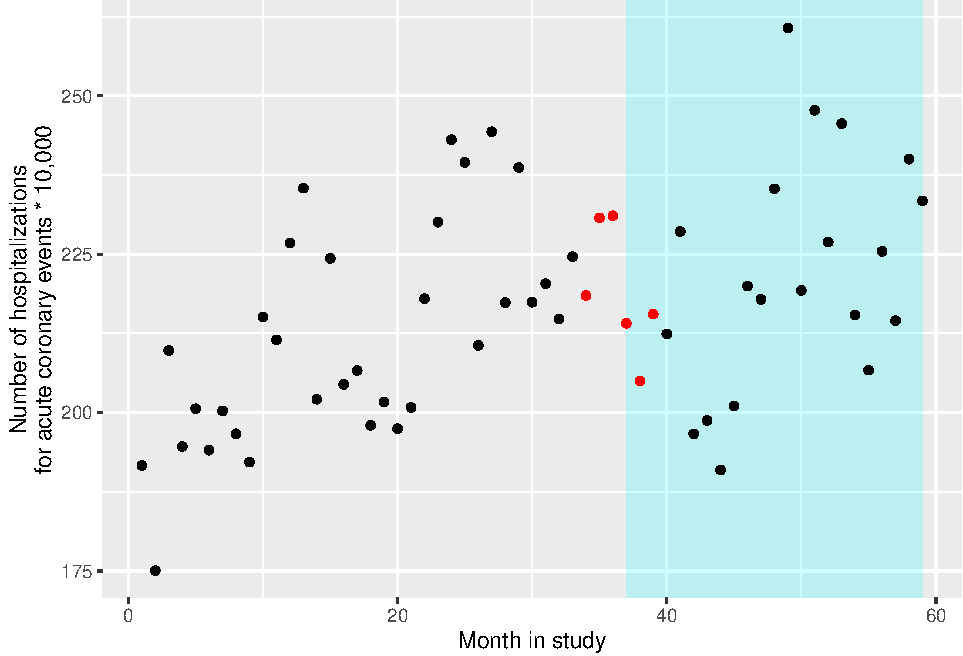
\includegraphics{adv_epi_analysis_files/figure-latex/unnamed-chunk-127-1.pdf}

Next, let's compare the rates of the outcome in these two groups: ``untreated'' (i.e., right before the date of the ban) and ``treated'' (i.e., right after the date of the ban). We can use a GLM to do this. It might seem somewhat like overkill---we could typically use a simpler statistical framework to determine the difference in two groups. However, using the GLM framework gets the job done even for a simple comparison, with the added benefit that it gives us room to expand as we think about adding control for some other factors. Further, it allows us to do some nice things like add an offset for the population size and allow for overdispersion.

To allow for overdispersion, we'll do the same thing we did in earlier chapters---we'll use the ``quasipoisson'' family when setting up the regression equation. This will have R estimate an additional parameter, one that estimates an overdispersion parameter for the data. For the population offset, we can incorporate that using the \texttt{offset} function. We'll take the log of the standardized population, so it will have the same transformation as the outcome variable in this structure (remember that, for Poisson GLMs, the link is a log). By wrapping it in \texttt{offset} when we include it in the model equation, we're telling R something special---it should include this variable in the structure of the equation when it fits the data, but it should not estimate a coefficient for it (as it will for everything else on the right side of the \texttt{\textasciitilde{}} in the nodel statement).

Here is the code you can use to fit this regression model:

\begin{Shaded}
\begin{Highlighting}[]
\NormalTok{near\_thres\_mod }\OtherTok{\textless{}{-}} \FunctionTok{glm}\NormalTok{(aces }\SpecialCharTok{\textasciitilde{}} \FunctionTok{offset}\NormalTok{(}\FunctionTok{log}\NormalTok{(stdpop)) }\SpecialCharTok{+}\NormalTok{ smokban, }
                      \AttributeTok{data =}\NormalTok{ near\_threshold, }
                      \AttributeTok{family =} \StringTok{"quasipoisson"}\NormalTok{)}
\end{Highlighting}
\end{Shaded}

The model equation for the model you are fitting with this code is:

\[
log(E(Y_t)) = \beta_0 + \beta_1 X_t + log(StdPop_t)
\]
(Note that there is no paratemer for the offset term!) We can rearrange this as:

\[
log(E(Y_t)) - log(StdPop_t) = \beta_0 + \beta_1 X_t 
\]
And based on the properties of logarithmic functions the above is equivalent to this which is essenntially a model for rates

\[
log(E(Y_t/StdPop_t)) = \beta_0 + \beta_1 X_t 
\]

\(E(Y/Std.Pop.)\) is the expected rate of outcome \(Y\) on day \(t\) (the \(StdPop_t\) in the denominator makes this a rate based on the standardize population size that day rather than just a count), \(\beta_0\) is a model intercept, \(X_t\) is an indicator variable that is 1 after the ban and 0 before the ban, and \(\beta_1\) is the estimate of the log rate ratio after the ban versus before the ban.

You can use the same technique as always to extract the estimates of the coefficients (again, notice that you don't get one for the offset term!):

\begin{Shaded}
\begin{Highlighting}[]
\FunctionTok{library}\NormalTok{(broom)}
\NormalTok{near\_thres\_mod }\SpecialCharTok{\%\textgreater{}\%} 
  \FunctionTok{tidy}\NormalTok{()}
\end{Highlighting}
\end{Shaded}

\begin{verbatim}
## # A tibble: 2 x 5
##   term        estimate std.error statistic  p.value
##   <chr>          <dbl>     <dbl>     <dbl>    <dbl>
## 1 (Intercept)  -6.09      0.0168   -362.   3.49e-10
## 2 smokban      -0.0695    0.0241     -2.88 4.51e- 2
\end{verbatim}

Based on these, there is a decrease in rates of ACE after the smoking ban, and we would reject the null hypothesis that the size of the change in rates post- versus pre-ban is 0 (because the p-value is lower than 0.05, although barely).

From these estimates, we can also get an estimate of the relative rate for the
group right after the ban versus right before the ban, as well as the 95\% confidence intervals for that estimate. Since we only have a few data points (6), we shouldn't use 1.96 in calculating the confidence intervals, but instead get the right value for our sample size using \texttt{qt}, which allows us to get quantiles of interest from the (student's) t-distribution. (The 1.96, is taken from the standard normal distribution (z-scores), but because of out small sample size n=6 the t-distribution will deviate considerably for that)) Since we have 6 data points and are estimating one coefficient plus the intercept, we have 6 - 2 degrees of freedom for this comparison:

\begin{Shaded}
\begin{Highlighting}[]
\NormalTok{near\_thres\_mod }\SpecialCharTok{\%\textgreater{}\%} 
  \FunctionTok{tidy}\NormalTok{() }\SpecialCharTok{\%\textgreater{}\%} 
  \FunctionTok{filter}\NormalTok{(term }\SpecialCharTok{==} \StringTok{"smokban"}\NormalTok{) }\SpecialCharTok{\%\textgreater{}\%} 
  \FunctionTok{mutate}\NormalTok{(}\AttributeTok{rr =} \FunctionTok{exp}\NormalTok{(estimate), }
         \AttributeTok{low\_rr =} \FunctionTok{exp}\NormalTok{(estimate }\SpecialCharTok{+} \FunctionTok{qt}\NormalTok{(}\FloatTok{0.025}\NormalTok{, }\AttributeTok{df =} \DecValTok{4}\NormalTok{) }\SpecialCharTok{*}\NormalTok{ std.error), }
         \AttributeTok{high\_rr =} \FunctionTok{exp}\NormalTok{(estimate }\SpecialCharTok{+} \FunctionTok{qt}\NormalTok{(}\FloatTok{0.975}\NormalTok{, }\AttributeTok{df =} \DecValTok{4}\NormalTok{) }\SpecialCharTok{*}\NormalTok{ std.error)) }\SpecialCharTok{\%\textgreater{}\%} 
  \FunctionTok{select}\NormalTok{(rr, low\_rr, high\_rr)}
\end{Highlighting}
\end{Shaded}

\begin{verbatim}
## # A tibble: 1 x 3
##      rr low_rr high_rr
##   <dbl>  <dbl>   <dbl>
## 1 0.933  0.872   0.998
\end{verbatim}

(We can check the quantilies of the t-distriution for 4 df, if we want to see how far away from the 1.96 value we are)

\begin{Shaded}
\begin{Highlighting}[]
\FunctionTok{qt}\NormalTok{(}\FloatTok{0.025}\NormalTok{, }\AttributeTok{df =} \DecValTok{4}\NormalTok{)}
\end{Highlighting}
\end{Shaded}

\begin{verbatim}
## [1] -2.776445
\end{verbatim}

\begin{Shaded}
\begin{Highlighting}[]
\FunctionTok{qt}\NormalTok{(}\FloatTok{0.975}\NormalTok{, }\AttributeTok{df =} \DecValTok{4}\NormalTok{) }
\end{Highlighting}
\end{Shaded}

\begin{verbatim}
## [1] 2.776445
\end{verbatim}

We can see that \(\pm 1.96\) would have given us deceptively narrower CIs

Now we can try some larger windows. Here is the analysis for 6 month-windows
on either side of the ban. The only things that change are the window for selecting data to include and the degrees of freedom used when calculating confidence intervals:

\begin{Shaded}
\begin{Highlighting}[]
\NormalTok{near\_threshold2 }\OtherTok{\textless{}{-}}\NormalTok{ sicily }\SpecialCharTok{\%\textgreater{}\%} 
  \FunctionTok{filter}\NormalTok{(time }\SpecialCharTok{\%in\%} \DecValTok{31}\SpecialCharTok{:}\DecValTok{42}\NormalTok{)}
\NormalTok{near\_thres\_mod2 }\OtherTok{\textless{}{-}} \FunctionTok{glm}\NormalTok{(aces }\SpecialCharTok{\textasciitilde{}} \FunctionTok{offset}\NormalTok{(}\FunctionTok{log}\NormalTok{(stdpop)) }\SpecialCharTok{+}\NormalTok{ smokban, }
                      \AttributeTok{data =}\NormalTok{ near\_threshold2, }
                      \AttributeTok{family =} \StringTok{"quasipoisson"}\NormalTok{)}
\NormalTok{near\_thres\_mod2 }\SpecialCharTok{\%\textgreater{}\%} 
  \FunctionTok{tidy}\NormalTok{()}
\end{Highlighting}
\end{Shaded}

\begin{verbatim}
## # A tibble: 2 x 5
##   term        estimate std.error statistic  p.value
##   <chr>          <dbl>     <dbl>     <dbl>    <dbl>
## 1 (Intercept)  -6.10      0.0167   -366.   5.74e-22
## 2 smokban      -0.0520    0.0239     -2.18 5.43e- 2
\end{verbatim}

\begin{Shaded}
\begin{Highlighting}[]
\NormalTok{near\_thres\_mod2 }\SpecialCharTok{\%\textgreater{}\%} 
  \FunctionTok{tidy}\NormalTok{() }\SpecialCharTok{\%\textgreater{}\%} 
  \FunctionTok{filter}\NormalTok{(term }\SpecialCharTok{==} \StringTok{"smokban"}\NormalTok{) }\SpecialCharTok{\%\textgreater{}\%} 
  \FunctionTok{mutate}\NormalTok{(}\AttributeTok{rr =} \FunctionTok{exp}\NormalTok{(estimate), }
         \AttributeTok{low\_rr =} \FunctionTok{exp}\NormalTok{(estimate }\SpecialCharTok{+} \FunctionTok{qt}\NormalTok{(}\FloatTok{0.025}\NormalTok{, }\AttributeTok{df =} \DecValTok{10}\NormalTok{) }\SpecialCharTok{*}\NormalTok{ std.error), }
         \AttributeTok{high\_rr =} \FunctionTok{exp}\NormalTok{(estimate }\SpecialCharTok{+} \FunctionTok{qt}\NormalTok{(}\FloatTok{0.975}\NormalTok{, }\AttributeTok{df =} \DecValTok{10}\NormalTok{) }\SpecialCharTok{*}\NormalTok{ std.error)) }\SpecialCharTok{\%\textgreater{}\%} 
  \FunctionTok{select}\NormalTok{(rr, low\_rr, high\_rr)}
\end{Highlighting}
\end{Shaded}

\begin{verbatim}
## # A tibble: 1 x 3
##      rr low_rr high_rr
##   <dbl>  <dbl>   <dbl>
## 1 0.949  0.900    1.00
\end{verbatim}

Here is the analysis for 12 month-windows
on either side of the ban. Again, the only things that change are the window for selecting data to include and the degrees of freedom used when calculating confidence intervals:

\begin{Shaded}
\begin{Highlighting}[]
\NormalTok{near\_threshold3 }\OtherTok{\textless{}{-}}\NormalTok{ sicily }\SpecialCharTok{\%\textgreater{}\%} 
  \FunctionTok{filter}\NormalTok{(time }\SpecialCharTok{\%in\%} \DecValTok{25}\SpecialCharTok{:}\DecValTok{48}\NormalTok{)}
\NormalTok{near\_thres\_mod3 }\OtherTok{\textless{}{-}} \FunctionTok{glm}\NormalTok{(aces }\SpecialCharTok{\textasciitilde{}} \FunctionTok{offset}\NormalTok{(}\FunctionTok{log}\NormalTok{(stdpop)) }\SpecialCharTok{+}\NormalTok{ smokban, }
                      \AttributeTok{data =}\NormalTok{ near\_threshold3, }
                      \AttributeTok{family =} \StringTok{"quasipoisson"}\NormalTok{)}
\NormalTok{near\_thres\_mod3 }\SpecialCharTok{\%\textgreater{}\%} 
  \FunctionTok{tidy}\NormalTok{()}
\end{Highlighting}
\end{Shaded}

\begin{verbatim}
## # A tibble: 2 x 5
##   term        estimate std.error statistic  p.value
##   <chr>          <dbl>     <dbl>     <dbl>    <dbl>
## 1 (Intercept)  -6.09      0.0160   -382.   1.56e-43
## 2 smokban      -0.0656    0.0229     -2.86 9.04e- 3
\end{verbatim}

\begin{Shaded}
\begin{Highlighting}[]
\NormalTok{near\_thres\_mod3 }\SpecialCharTok{\%\textgreater{}\%} 
  \FunctionTok{tidy}\NormalTok{() }\SpecialCharTok{\%\textgreater{}\%} 
  \FunctionTok{filter}\NormalTok{(term }\SpecialCharTok{==} \StringTok{"smokban"}\NormalTok{) }\SpecialCharTok{\%\textgreater{}\%} 
  \FunctionTok{mutate}\NormalTok{(}\AttributeTok{rr =} \FunctionTok{exp}\NormalTok{(estimate), }
         \AttributeTok{low\_rr =} \FunctionTok{exp}\NormalTok{(estimate }\SpecialCharTok{+} \FunctionTok{qt}\NormalTok{(}\FloatTok{0.025}\NormalTok{, }\AttributeTok{df =} \DecValTok{22}\NormalTok{) }\SpecialCharTok{*}\NormalTok{ std.error), }
         \AttributeTok{high\_rr =} \FunctionTok{exp}\NormalTok{(estimate }\SpecialCharTok{+} \FunctionTok{qt}\NormalTok{(}\FloatTok{0.975}\NormalTok{, }\AttributeTok{df =} \DecValTok{22}\NormalTok{) }\SpecialCharTok{*}\NormalTok{ std.error)) }\SpecialCharTok{\%\textgreater{}\%} 
  \FunctionTok{select}\NormalTok{(rr, low\_rr, high\_rr)}
\end{Highlighting}
\end{Shaded}

\begin{verbatim}
## # A tibble: 1 x 3
##      rr low_rr high_rr
##   <dbl>  <dbl>   <dbl>
## 1 0.937  0.893   0.982
\end{verbatim}

As we look at these different windows, we don't see much change in the estimated relative rate of the outcome after the ban versus before. However, our estimate of this relative rate is becoming more precise as it's estimated with more data points.

However, eventually we may run into problems with residual confounding. As we include data further and further from the threshold (the date of the ban), we have more and more problems with the assumption that the data before and after the threshold are comprable for any factors other than the status of the smoking ban. In particular, we're opening up more and more possibility for our estimate to be affected by residual confounding by long-term trends in the outcome rate over the study period as we include a wider window of days in that study period. In the next section, we'll look at how we can add control for a long-term trend to the model, so we can use all of the data while controlling for potential long-term trends, thus reducing the risk of residual confounding by them.

\begin{enumerate}
\def\labelenumi{\arabic{enumi}.}
\setcounter{enumi}{2}
\tightlist
\item
  \textbf{Now see if you can fit a regression model that uses all the data, while using a regression term to allow for a long-term trend in the rates of the outcome. You may want to try out several of the model structures shown in Figure 2 of \citet{bernal2017interrupted}. Can you interpret the model coefficients that you get from fitting these models? What conclusions do you draw about whether rates of hospitalization for acute coronary events are affected by exposure to secondary smoke?}
\end{enumerate}

Now we will fit a full regression model for an interrupted time series. We will add a term to fit a trend for steady trends along the forcing variable. For interrupted time series, that forcing variable is time, so we'll be adding a term to control for trends long-term in time. However, this general idea can be used with any type of regression discontinuity study design, some of which will have forcing variables other than time.

To add a trend for time---as long as we're willing to assume that the trend isn't changed when the ban takes effect, just that there is a ``hop'' in the trend line to account for an immediate change in rates---we can just add a term to our regression model. We'll now fit the following regression model:

\[
log(E(Y_t/StdPop_t)) = \beta_0 + \beta_1 X_t + \beta_2 T
\]

where all the terms are the same as in the last section, while now a linear term has been added for month in study (time; \(T\)) with an associated coefficient \(\beta_2\). In \citet{bernal2017interrupted}, this corresponds to the model structure shown in panel (a) of Figure 2: There is an ``interruption'' at the time of the ban, and there is a long-term trend in the outcome rates regardless of this ban, but the ban only creates the immediate interruption, without changing the shape of the long-term trend.

Below is the code that will fit this model in R. We'll change the \texttt{data} argument to now include all available data points. The other change is that we're adding a linear term for time (\texttt{time}).

\begin{Shaded}
\begin{Highlighting}[]
\NormalTok{int\_ts\_mod1 }\OtherTok{\textless{}{-}} \FunctionTok{glm}\NormalTok{(aces }\SpecialCharTok{\textasciitilde{}} \FunctionTok{offset}\NormalTok{(}\FunctionTok{log}\NormalTok{(stdpop)) }\SpecialCharTok{+}\NormalTok{ smokban }\SpecialCharTok{+}\NormalTok{ time, }
                      \AttributeTok{data =}\NormalTok{ sicily, }
                      \AttributeTok{family =} \StringTok{"quasipoisson"}\NormalTok{)}
\end{Highlighting}
\end{Shaded}

We can look at the results from fitting this model, using the same technique as in the last section:

\begin{Shaded}
\begin{Highlighting}[]
\NormalTok{int\_ts\_mod1 }\SpecialCharTok{\%\textgreater{}\%} 
  \FunctionTok{tidy}\NormalTok{()}
\end{Highlighting}
\end{Shaded}

\begin{verbatim}
## # A tibble: 3 x 5
##   term        estimate std.error statistic  p.value
##   <chr>          <dbl>     <dbl>     <dbl>    <dbl>
## 1 (Intercept) -6.24     0.0211     -296.   3.94e-91
## 2 smokban     -0.112    0.0325       -3.44 1.12e- 3
## 3 time         0.00494  0.000942      5.25 2.43e- 6
\end{verbatim}

\begin{Shaded}
\begin{Highlighting}[]
\NormalTok{int\_ts\_mod1 }\SpecialCharTok{\%\textgreater{}\%} 
  \FunctionTok{tidy}\NormalTok{() }\SpecialCharTok{\%\textgreater{}\%} 
  \FunctionTok{filter}\NormalTok{(term }\SpecialCharTok{==} \StringTok{"smokban"}\NormalTok{) }\SpecialCharTok{\%\textgreater{}\%} 
  \FunctionTok{mutate}\NormalTok{(}\AttributeTok{rr =} \FunctionTok{exp}\NormalTok{(estimate), }
         \AttributeTok{low\_rr =} \FunctionTok{exp}\NormalTok{(estimate }\SpecialCharTok{+} \FunctionTok{qt}\NormalTok{(}\FloatTok{0.025}\NormalTok{, }\AttributeTok{df =} \DecValTok{56}\NormalTok{) }\SpecialCharTok{*}\NormalTok{ std.error), }
         \AttributeTok{high\_rr =} \FunctionTok{exp}\NormalTok{(estimate }\SpecialCharTok{+} \FunctionTok{qt}\NormalTok{(}\FloatTok{0.975}\NormalTok{, }\AttributeTok{df =} \DecValTok{56}\NormalTok{) }\SpecialCharTok{*}\NormalTok{ std.error)) }\SpecialCharTok{\%\textgreater{}\%} 
  \FunctionTok{select}\NormalTok{(rr, low\_rr, high\_rr)}
\end{Highlighting}
\end{Shaded}

\begin{verbatim}
## # A tibble: 1 x 3
##      rr low_rr high_rr
##   <dbl>  <dbl>   <dbl>
## 1 0.894  0.838   0.955
\end{verbatim}

These results show us a few things. First, there is clearly a long-term time trend---the p value on the ``time'' coefficient estimate is much lower than 0.05. Second, the estimated benefit from the smoking ban, in terms of reducing rates of ACE hospitalization, is a bit stronger when we control for long-term trends. We are now estimating about a 11\% decrease in hospitalization rates in association with this indoor smoking ban. It's possible that our results in the last sections were somewhat confounded by long-term trends.

\begin{Shaded}
\begin{Highlighting}[]
\NormalTok{mod\_data }\OtherTok{\textless{}{-}}\NormalTok{ int\_ts\_mod1 }\SpecialCharTok{\%\textgreater{}\%} 
  \FunctionTok{augment}\NormalTok{() }\SpecialCharTok{\%\textgreater{}\%} 
  \FunctionTok{mutate}\NormalTok{(}\AttributeTok{stdpop =}\NormalTok{ sicily}\SpecialCharTok{$}\NormalTok{stdpop,}
         \AttributeTok{aces\_adj =}\NormalTok{ aces }\SpecialCharTok{/}\NormalTok{ stdpop }\SpecialCharTok{*}\NormalTok{ (}\DecValTok{10} \SpecialCharTok{\^{}} \DecValTok{5}\NormalTok{)) }
\FunctionTok{ggplot}\NormalTok{() }\SpecialCharTok{+}  
  \FunctionTok{geom\_polygon}\NormalTok{(}\FunctionTok{aes}\NormalTok{(}\AttributeTok{x =} \FunctionTok{c}\NormalTok{(}\DecValTok{37}\NormalTok{, }\DecValTok{59}\NormalTok{, }\DecValTok{59}\NormalTok{, }\DecValTok{37}\NormalTok{), }
                   \AttributeTok{y =} \FunctionTok{c}\NormalTok{(}\ConstantTok{Inf}\NormalTok{, }\ConstantTok{Inf}\NormalTok{, }\SpecialCharTok{{-}}\ConstantTok{Inf}\NormalTok{, }\SpecialCharTok{{-}}\ConstantTok{Inf}\NormalTok{)), }
               \AttributeTok{fill =} \StringTok{"cyan"}\NormalTok{, }\AttributeTok{alpha =} \FloatTok{0.2}\NormalTok{) }\SpecialCharTok{+}
  \FunctionTok{geom\_point}\NormalTok{(}\AttributeTok{data =}\NormalTok{ mod\_data, }\FunctionTok{aes}\NormalTok{(}\AttributeTok{x =}\NormalTok{ time, }
                                  \AttributeTok{y =}\NormalTok{ aces }\SpecialCharTok{/}\NormalTok{ stdpop }\SpecialCharTok{*}\NormalTok{ (}\DecValTok{10} \SpecialCharTok{\^{}} \DecValTok{5}\NormalTok{))) }\SpecialCharTok{+} 
  \FunctionTok{geom\_line}\NormalTok{(}\AttributeTok{data =}\NormalTok{ mod\_data, }\FunctionTok{aes}\NormalTok{(}\AttributeTok{x =}\NormalTok{ time, }
                                 \AttributeTok{y =} \FunctionTok{exp}\NormalTok{(.fitted) }\SpecialCharTok{/}\NormalTok{ stdpop }\SpecialCharTok{*}\NormalTok{ (}\DecValTok{10} \SpecialCharTok{\^{}} \DecValTok{5}\NormalTok{)), }
            \AttributeTok{color =} \StringTok{"red"}\NormalTok{)}
\end{Highlighting}
\end{Shaded}

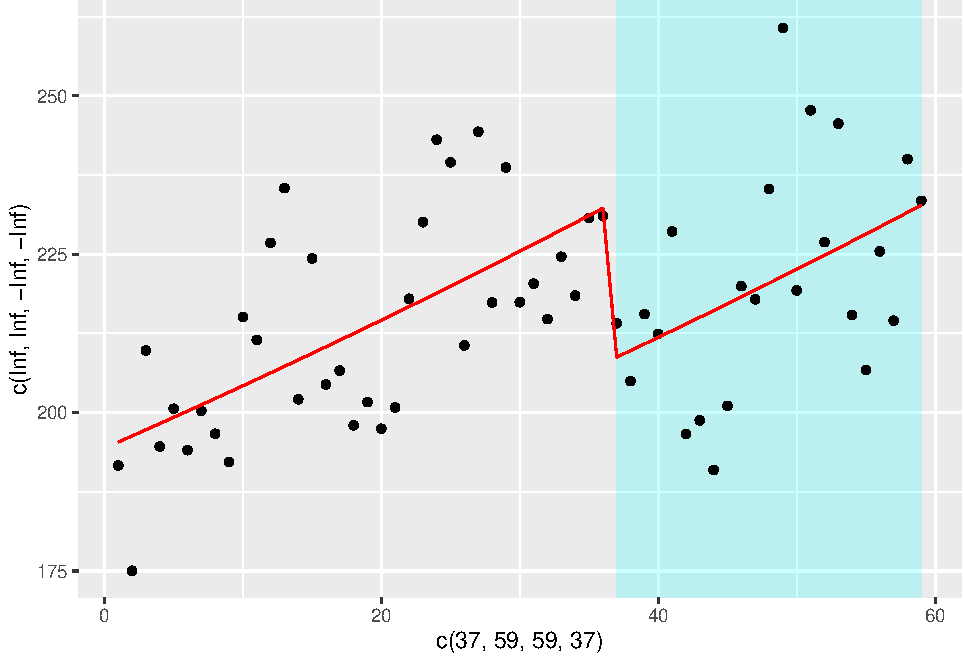
\includegraphics{adv_epi_analysis_files/figure-latex/unnamed-chunk-136-1.pdf}

Next, we can try to fit the model stucture that is shown in panel (c) of Figure 2 in \citet{bernal2017interrupted}. This structure includes an abrupt interruption when the ban is introduced, as well as a change in the slope of the long-term trend following the ban.

The structure of this regression model will include an extra term, to allow the slope of the long-term trend to change after the ban. The model is:

\[
log(E(Y_t/StdPop_t)) = \beta_0 + \beta_1 X_t + \beta_2 T + \beta_3 (T-T_0)X_t
\]

where \((T-T_0)\) is a measure of time since the date of the ban and \(\beta_3\) allows for a change in the slope of the time trend line after the ban. (As a note, \((T-T_0)X_t\) could also be expressed as \((T-T_0)_+\) using the \((..)_+\) notation we introduced last week.)

To fit this model in R, you can run:

\begin{Shaded}
\begin{Highlighting}[]
\NormalTok{int\_ts\_mod2 }\OtherTok{\textless{}{-}} \FunctionTok{glm}\NormalTok{(aces }\SpecialCharTok{\textasciitilde{}} \FunctionTok{offset}\NormalTok{(}\FunctionTok{log}\NormalTok{(stdpop)) }\SpecialCharTok{+}\NormalTok{ smokban }\SpecialCharTok{+}\NormalTok{ time }\SpecialCharTok{+} 
                     \FunctionTok{I}\NormalTok{(time }\SpecialCharTok{{-}} \DecValTok{36}\NormalTok{)}\SpecialCharTok{:}\NormalTok{smokban, }
                      \AttributeTok{data =}\NormalTok{ sicily, }
                      \AttributeTok{family =} \StringTok{"quasipoisson"}\NormalTok{)}
\end{Highlighting}
\end{Shaded}

\begin{Shaded}
\begin{Highlighting}[]
\NormalTok{int\_ts\_mod2 }\SpecialCharTok{\%\textgreater{}\%} 
  \FunctionTok{tidy}\NormalTok{()}
\end{Highlighting}
\end{Shaded}

\begin{verbatim}
## # A tibble: 4 x 5
##   term                  estimate std.error statistic  p.value
##   <chr>                    <dbl>     <dbl>     <dbl>    <dbl>
## 1 (Intercept)          -6.24       0.0233   -268.    2.31e-87
## 2 smokban              -0.114      0.0356     -3.21  2.23e- 3
## 3 time                  0.00485    0.00107     4.52  3.28e- 5
## 4 smokban:I(time - 36)  0.000417   0.00231     0.181 8.57e- 1
\end{verbatim}

\begin{Shaded}
\begin{Highlighting}[]
\NormalTok{int\_ts\_mod1 }\SpecialCharTok{\%\textgreater{}\%} 
  \FunctionTok{tidy}\NormalTok{() }\SpecialCharTok{\%\textgreater{}\%} 
  \FunctionTok{filter}\NormalTok{(term }\SpecialCharTok{==} \StringTok{"smokban"}\NormalTok{) }\SpecialCharTok{\%\textgreater{}\%} 
  \FunctionTok{mutate}\NormalTok{(}\AttributeTok{rr =} \FunctionTok{exp}\NormalTok{(estimate), }
         \AttributeTok{low\_rr =} \FunctionTok{exp}\NormalTok{(estimate }\SpecialCharTok{+} \FunctionTok{qt}\NormalTok{(}\FloatTok{0.025}\NormalTok{, }\AttributeTok{df =} \DecValTok{55}\NormalTok{) }\SpecialCharTok{*}\NormalTok{ std.error), }
         \AttributeTok{high\_rr =} \FunctionTok{exp}\NormalTok{(estimate }\SpecialCharTok{+} \FunctionTok{qt}\NormalTok{(}\FloatTok{0.975}\NormalTok{, }\AttributeTok{df =} \DecValTok{55}\NormalTok{) }\SpecialCharTok{*}\NormalTok{ std.error)) }\SpecialCharTok{\%\textgreater{}\%} 
  \FunctionTok{select}\NormalTok{(rr, low\_rr, high\_rr)}
\end{Highlighting}
\end{Shaded}

\begin{verbatim}
## # A tibble: 1 x 3
##      rr low_rr high_rr
##   <dbl>  <dbl>   <dbl>
## 1 0.894  0.838   0.955
\end{verbatim}

Based on these results, there is not a statistically significant change in the slope of the time trend after the ban compared to before (i.e., a p-value of 0.18 for testing against the null that this coefficient is 0). We get a very similar estimate of the abrupt change in ACE rates right when the ban was implemented as compared to the simpler model we fit without a term for change in slope of the long-term time trends.

\begin{enumerate}
\def\labelenumi{\arabic{enumi}.}
\setcounter{enumi}{3}
\tightlist
\item
  \textbf{Now let's try to control for long-term and seasonal trends beyond the linear term for time. Fit a model using a harmonic term like in \citet{bernal2017interrupted}. Do the coefficients from the model for the smoking ban and linear time term change? In previous examples, we've been using flexible functions for this such as splines. Repeat the model from above using a spline term. How does this model compare with respect to the smoking ban coefficient? Why?}
\end{enumerate}

We've been adjusting for long-term and seasonal trends using a flexible spline term so far. Let's try and incorporate this in the mode here. Here we will try a new function from the \texttt{tsModel} package called \texttt{harmonic}. The \texttt{harmonic} function will fit pairs of sine and cosine functions in a given period of time. Here we will define the function as \texttt{harmonic(month,2,12)} fitting two pairs of sine and cosine functions over a 12-month period. These combined sine and cosine functions create a sinusoidal patten with peaks and troughs that we've seen for seasonal treands previously.

\begin{Shaded}
\begin{Highlighting}[]
\FunctionTok{library}\NormalTok{(tsModel)}
\NormalTok{int\_ts\_mod3 }\OtherTok{\textless{}{-}} \FunctionTok{glm}\NormalTok{(aces }\SpecialCharTok{\textasciitilde{}} \FunctionTok{offset}\NormalTok{(}\FunctionTok{log}\NormalTok{(stdpop)) }\SpecialCharTok{+}\NormalTok{ smokban }\SpecialCharTok{+}\NormalTok{ time }\SpecialCharTok{+} 
                     \FunctionTok{I}\NormalTok{(time }\SpecialCharTok{{-}} \DecValTok{36}\NormalTok{)}\SpecialCharTok{:}\NormalTok{smokban }\SpecialCharTok{+} \FunctionTok{harmonic}\NormalTok{(month,}\DecValTok{2}\NormalTok{,}\DecValTok{12}\NormalTok{), }
                      \AttributeTok{data =}\NormalTok{ sicily, }
                      \AttributeTok{family =} \StringTok{"quasipoisson"}\NormalTok{)}
\end{Highlighting}
\end{Shaded}

In order to visualize the effect of the harmonic function we can plot the predicted values from this model same as above:

\begin{Shaded}
\begin{Highlighting}[]
\NormalTok{mod\_data2 }\OtherTok{\textless{}{-}}\NormalTok{ int\_ts\_mod3 }\SpecialCharTok{\%\textgreater{}\%} 
  \FunctionTok{augment}\NormalTok{() }\SpecialCharTok{\%\textgreater{}\%} 
  \FunctionTok{mutate}\NormalTok{(}\AttributeTok{stdpop =}\NormalTok{ sicily}\SpecialCharTok{$}\NormalTok{stdpop,}
         \AttributeTok{aces\_adj =}\NormalTok{ aces }\SpecialCharTok{/}\NormalTok{ stdpop }\SpecialCharTok{*}\NormalTok{ (}\DecValTok{10} \SpecialCharTok{\^{}} \DecValTok{5}\NormalTok{)) }
\FunctionTok{ggplot}\NormalTok{() }\SpecialCharTok{+}  
  \FunctionTok{geom\_point}\NormalTok{(}\AttributeTok{data =}\NormalTok{ mod\_data2, }\FunctionTok{aes}\NormalTok{(}\AttributeTok{x =}\NormalTok{ time, }
                                  \AttributeTok{y =}\NormalTok{ aces }\SpecialCharTok{/}\NormalTok{ stdpop }\SpecialCharTok{*}\NormalTok{ (}\DecValTok{10} \SpecialCharTok{\^{}} \DecValTok{5}\NormalTok{))) }\SpecialCharTok{+} 
  \FunctionTok{geom\_line}\NormalTok{(}\AttributeTok{data =}\NormalTok{ mod\_data2, }\FunctionTok{aes}\NormalTok{(}\AttributeTok{x =}\NormalTok{ time, }
                                 \AttributeTok{y =} \FunctionTok{exp}\NormalTok{(.fitted) }\SpecialCharTok{/}\NormalTok{ stdpop }\SpecialCharTok{*}\NormalTok{ (}\DecValTok{10} \SpecialCharTok{\^{}} \DecValTok{5}\NormalTok{)), }
            \AttributeTok{color =} \StringTok{"red"}\NormalTok{)}
\end{Highlighting}
\end{Shaded}

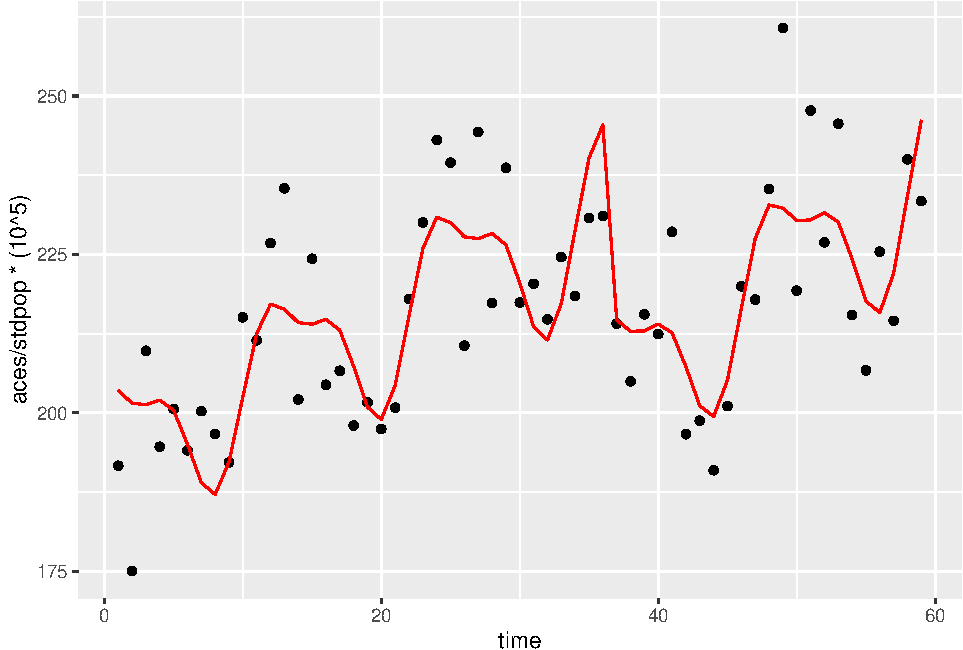
\includegraphics{adv_epi_analysis_files/figure-latex/unnamed-chunk-140-1.pdf}

We see that the addition of the harmonic term now yields a more flexible overall function over time. Now let's check how the coefficients for \texttt{smokban} and \texttt{time} changed if at all

\begin{Shaded}
\begin{Highlighting}[]
\NormalTok{int\_ts\_mod3 }\SpecialCharTok{\%\textgreater{}\%} 
  \FunctionTok{tidy}\NormalTok{()}
\end{Highlighting}
\end{Shaded}

\begin{verbatim}
## # A tibble: 8 x 5
##   term                    estimate std.error statistic  p.value
##   <chr>                      <dbl>     <dbl>     <dbl>    <dbl>
## 1 (Intercept)             -6.25     0.0189    -331.    1.20e-86
## 2 smokban                 -0.132    0.0298      -4.43  5.07e- 5
## 3 time                     0.00510  0.000875     5.83  3.72e- 7
## 4 harmonic(month, 2, 12)1  0.0383   0.0102       3.77  4.27e- 4
## 5 harmonic(month, 2, 12)2 -0.0176   0.00970     -1.82  7.49e- 2
## 6 harmonic(month, 2, 12)3  0.0384   0.00971      3.95  2.42e- 4
## 7 harmonic(month, 2, 12)4  0.0150   0.00975      1.53  1.31e- 1
## 8 smokban:I(time - 36)     0.00148  0.00185      0.799 4.28e- 1
\end{verbatim}

\begin{Shaded}
\begin{Highlighting}[]
\NormalTok{int\_ts\_mod3 }\SpecialCharTok{\%\textgreater{}\%} 
  \FunctionTok{tidy}\NormalTok{() }\SpecialCharTok{\%\textgreater{}\%} 
  \FunctionTok{filter}\NormalTok{(term }\SpecialCharTok{==} \StringTok{"smokban"}\NormalTok{) }\SpecialCharTok{\%\textgreater{}\%} 
  \FunctionTok{mutate}\NormalTok{(}\AttributeTok{rr =} \FunctionTok{exp}\NormalTok{(estimate), }
         \AttributeTok{low\_rr =} \FunctionTok{exp}\NormalTok{(estimate }\SpecialCharTok{+} \FunctionTok{qt}\NormalTok{(}\FloatTok{0.025}\NormalTok{, }\AttributeTok{df =} \DecValTok{51}\NormalTok{) }\SpecialCharTok{*}\NormalTok{ std.error), }
         \AttributeTok{high\_rr =} \FunctionTok{exp}\NormalTok{(estimate }\SpecialCharTok{+} \FunctionTok{qt}\NormalTok{(}\FloatTok{0.975}\NormalTok{, }\AttributeTok{df =} \DecValTok{51}\NormalTok{) }\SpecialCharTok{*}\NormalTok{ std.error)) }\SpecialCharTok{\%\textgreater{}\%} 
  \FunctionTok{select}\NormalTok{(rr, low\_rr, high\_rr)}
\end{Highlighting}
\end{Shaded}

\begin{verbatim}
## # A tibble: 1 x 3
##      rr low_rr high_rr
##   <dbl>  <dbl>   <dbl>
## 1 0.876  0.826   0.930
\end{verbatim}

The change in the slope of the time trend after the ban is still not statistically significant, but we see that the RR for the smoking ban term is actually marginally lower, meaning a slighlty more protetive effect after adjusting for the seasonal trends with a harmonic term.

Now why did we use this type of function as opposed to a spline? Let's repeat the model from above with a natural spline term as we had been doing in the previous example, with 30 df's (\textasciitilde6 per year).

\begin{Shaded}
\begin{Highlighting}[]
\FunctionTok{library}\NormalTok{(splines)}
\NormalTok{int\_ts\_mod4 }\OtherTok{\textless{}{-}} \FunctionTok{glm}\NormalTok{(aces }\SpecialCharTok{\textasciitilde{}} \FunctionTok{offset}\NormalTok{(}\FunctionTok{log}\NormalTok{(stdpop)) }\SpecialCharTok{+}\NormalTok{ smokban }\SpecialCharTok{+}\NormalTok{ time }\SpecialCharTok{+} 
                     \FunctionTok{I}\NormalTok{(time }\SpecialCharTok{{-}} \DecValTok{36}\NormalTok{)}\SpecialCharTok{:}\NormalTok{smokban }\SpecialCharTok{+} \FunctionTok{ns}\NormalTok{(time, }\AttributeTok{df=}\DecValTok{30}\NormalTok{), }
                      \AttributeTok{data =}\NormalTok{ sicily, }
                      \AttributeTok{family =} \StringTok{"quasipoisson"}\NormalTok{)}
\end{Highlighting}
\end{Shaded}

\begin{Shaded}
\begin{Highlighting}[]
\NormalTok{mod\_data3 }\OtherTok{\textless{}{-}}\NormalTok{ int\_ts\_mod4 }\SpecialCharTok{\%\textgreater{}\%} 
  \FunctionTok{augment}\NormalTok{() }\SpecialCharTok{\%\textgreater{}\%} 
  \FunctionTok{mutate}\NormalTok{(}\AttributeTok{stdpop =}\NormalTok{ sicily}\SpecialCharTok{$}\NormalTok{stdpop,}
         \AttributeTok{aces\_adj =}\NormalTok{ aces }\SpecialCharTok{/}\NormalTok{ stdpop }\SpecialCharTok{*}\NormalTok{ (}\DecValTok{10} \SpecialCharTok{\^{}} \DecValTok{5}\NormalTok{)) }
\FunctionTok{ggplot}\NormalTok{() }\SpecialCharTok{+}  
  \FunctionTok{geom\_point}\NormalTok{(}\AttributeTok{data =}\NormalTok{ mod\_data3, }\FunctionTok{aes}\NormalTok{(}\AttributeTok{x =}\NormalTok{ time, }
                                  \AttributeTok{y =}\NormalTok{ aces }\SpecialCharTok{/}\NormalTok{ stdpop }\SpecialCharTok{*}\NormalTok{ (}\DecValTok{10} \SpecialCharTok{\^{}} \DecValTok{5}\NormalTok{))) }\SpecialCharTok{+} 
  \FunctionTok{geom\_line}\NormalTok{(}\AttributeTok{data =}\NormalTok{ mod\_data3, }\FunctionTok{aes}\NormalTok{(}\AttributeTok{x =}\NormalTok{ time, }
                                 \AttributeTok{y =} \FunctionTok{exp}\NormalTok{(.fitted) }\SpecialCharTok{/}\NormalTok{ stdpop }\SpecialCharTok{*}\NormalTok{ (}\DecValTok{10} \SpecialCharTok{\^{}} \DecValTok{5}\NormalTok{)), }
            \AttributeTok{color =} \StringTok{"red"}\NormalTok{)}
\end{Highlighting}
\end{Shaded}

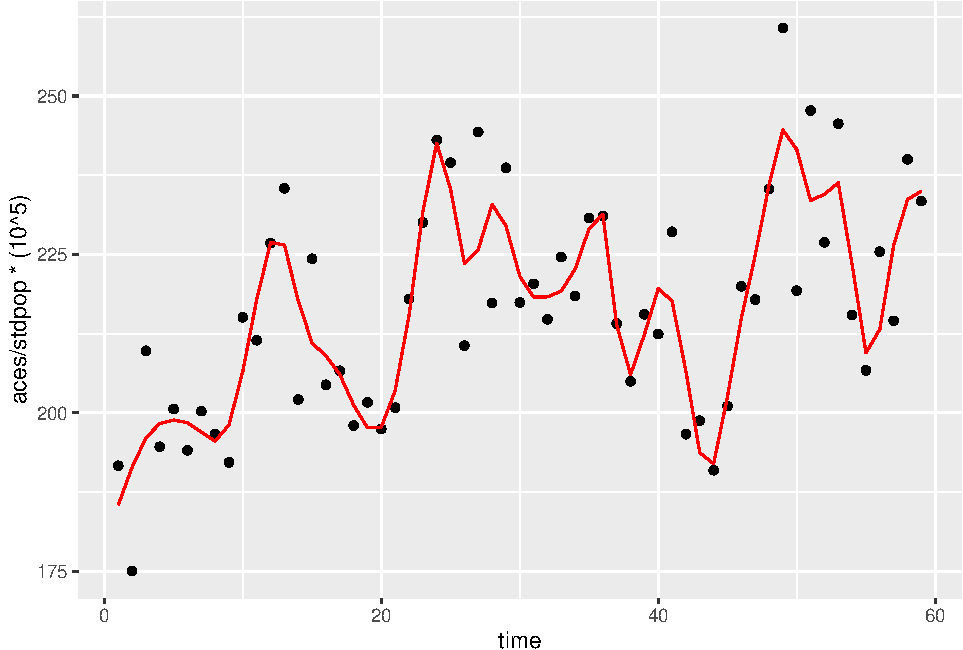
\includegraphics{adv_epi_analysis_files/figure-latex/unnamed-chunk-143-1.pdf}
We see that the spline term has succesfully fitted a flexible function over time. Now let's check the smoking ban RR

\begin{Shaded}
\begin{Highlighting}[]
\NormalTok{int\_ts\_mod4 }\SpecialCharTok{\%\textgreater{}\%} 
  \FunctionTok{tidy}\NormalTok{() }\SpecialCharTok{\%\textgreater{}\%} 
  \FunctionTok{filter}\NormalTok{(term }\SpecialCharTok{==} \StringTok{"smokban"}\NormalTok{) }\SpecialCharTok{\%\textgreater{}\%} 
  \FunctionTok{mutate}\NormalTok{(}\AttributeTok{rr =} \FunctionTok{exp}\NormalTok{(estimate), }
         \AttributeTok{low\_rr =} \FunctionTok{exp}\NormalTok{(estimate }\SpecialCharTok{+} \FunctionTok{qt}\NormalTok{(}\FloatTok{0.025}\NormalTok{, }\AttributeTok{df =} \DecValTok{25}\NormalTok{) }\SpecialCharTok{*}\NormalTok{ std.error), }
         \AttributeTok{high\_rr =} \FunctionTok{exp}\NormalTok{(estimate }\SpecialCharTok{+} \FunctionTok{qt}\NormalTok{(}\FloatTok{0.975}\NormalTok{, }\AttributeTok{df =} \DecValTok{25}\NormalTok{) }\SpecialCharTok{*}\NormalTok{ std.error)) }\SpecialCharTok{\%\textgreater{}\%} 
  \FunctionTok{select}\NormalTok{(rr, low\_rr, high\_rr)}
\end{Highlighting}
\end{Shaded}

\begin{verbatim}
## # A tibble: 1 x 3
##      rr low_rr high_rr
##   <dbl>  <dbl>   <dbl>
## 1  1.00  0.632    1.59
\end{verbatim}

The RR for the smoking ban term is now null. A richly parameterized spline term with a lot of degrees of freedom is actually too felxible a function for this analysis. Because of all the flexibility we are affording it, it is absorbing the drop in ACE rates occurring immediately after the ban in the overall function for time. Although spline functions and their flexibility can be an invaluable tool in modeling complex exposure-respone relationships, in this case it actually masked the effect of interest.

\chapter{Estimating health impacts}\label{estimating-health-impacts}

\section{Readings}\label{readings-3}

The readings for this chapter are:

\begin{itemize}
\tightlist
\item
  \citet{balbus2016climate} Overview on climate change and human health, including a section on quantifying health impacts. The first chapter in a report on climate change and human health by the US Global Change Research Program.
\item
  \citet{steenland2006overview} (Just the section on attributable fraction) Overview on estimating burden of disease through measures like attributable risk and attributable number (Note: The equation for \(AF_{pop}\) in this paper in equation 3 aligns with the equations for attributable risk described in this chapter)
\item
  \citet{gasparrini2014attributable} Calculating attributable risk from distributed lag non-linear models. Example code is included for this paper.
\item
  \citet{vicedo2019hands} Provides a tutorial of all the steps for a
  projecting of health impacts of temperature extremes under climate change.
\end{itemize}

The following are supplemental readings (i.e., not required, but may be of
interest) associated with the material in this chapter:

\begin{itemize}
\tightlist
\item
  \citet{kinney2008approaches} A review of challenges and approaches for projecting heat-related deaths under climate change
\item
  \citet{benichou2006attributable} Encyclopedia entry on attributable risk
\item
  \citet{northridge1995public} Brief summary of attributable risk with examples from epidemiology
\item
  \citet{greenland1988conceptual} Definition and interpretation of attributable fractions
\end{itemize}

\section{Attributable risk and attributable number}\label{attributable-risk-and-attributable-number}

So far, we have focused on estimating the relative risk of exposure on a health outcome. In some cases---where we can assume a linear relationship between the exposure and the log counts of the outcome---we were able to get a single measure of the relative risk per unit change of the exposure. In this case, the single measure of relative risk applies to a one-unit change anywhere along the range of exposure observed for the population. One common example is the association between outdoor particulate matter concentration and mortality, which is typically modeled using a linear association, resulting in a single estimate of relative risk per unit increase in the exposure (as a note, this ``unit'' can be any constant change in the exposure---often it will be selected to reflect a realistically important change in the exposure, for example, an increase of \(10 \mu g/m^3\) for \(PM_{2.5}\)).

We have also looked at some more complex cases, where we've used a non-linear function of the exposure to model associated risk of the health outcome. In these cases, it becomes a bit more complicated to interpret the results. First, you need to identify a ``baseline'' of exposure to use as a comparison for measurements of relative risk. While for a linear association, you can measure a relative risk per unit change, regardless of where the change happens along the range of exposure, for a non-linear association, you must pick specific points to compare, and a unit change in exposure will vary across the range of exposure. For example, when looking at temperature and mortality in London, we compared risk at specific high and low temperatures to a baseline at a mild, ``safe'' temperature, one where mortality risk was observed to be at its lowest. In other words, we selected a baseline level of exposure to use as a reference and then compared relative risk at ``slices'' of the non-linear exposure-response function to get summaries of the observed relative risk. As we moved to cross-basis functions, we similarly took ``slices'' to look at risk at specific lags or specific temperatures.

These techniques point towards a general theme---when we are studying how an environmental exposure is associated with risk of a health outcome, we need to not only fit an appropriate statistical model to describe the association, but we also need to extract some summaries from that model that we can use to communicate what we've found. Not only is this important for communicating our findings, it's also critical for making sure our findings can be used to improve public health.

So far, we have focused on summarizing and communicating our results based on estimates of relative risk. These estimates are a common summary in published environmental epidemiology studies, and they're helpful in identifying how levels of an exposure translate to increased health risk. However, they fail to incorporate one facet that is very important when trying to translate findings to public health impacts---they do not incorporate how common or rare exposures of different levels are in real life. For example, say you fit a model that shows an exposure-response function for temperature and mortality that is very flat everywhere except at very high temperatures. If those very high temperatures occur often (say, 20 days a year on average), then temperature would cause many more excess deaths in the community compared to if those temperatures are very rare (say, 1 day every five years on average). In other words, to interpret the public health impact of an exposure, you need to consider not only how health risk changes with the level of the exposure, but also how frequently different levels of exposure occur.

One epidemiological measure that incorporates these two facets is the measure of \textbf{attributable risk}. Attributable risk aims to measure the proportion of cases of disease in a population that is attributable to an exposure---in other words, what proportion of cases would you have avoided in a population if the exposure were eliminated (or, in cases where that doesn't make sense like temperature, held at its safest level)? A number of other terms are sometimes also used to describe this idea, including \emph{population attributable risk}, \emph{attributable fraction}. \emph{Etiological} or \emph{etiologic fraction} also appears in the literature as an equivalent or interchangeable term to \emph{attributable fraction}, but as Greenland and Robins point out \citep{greenland1988conceptual} the interpretation of each is more nuanced, and the two are not necessarily the same quantity.

In the simple case of a binary exposure (in other words, everyone in the study population can either be exposed or unexposed, but there aren't different levels of exposure), the attributable risk (\(AR\)) can be expressed mathematically as:

\[
AR = \frac{Pr(D) - Pr(D|\bar{E})}{Pr(D)}
\]
where \(Pr(D)\) is the probability of the disease in the population and \(Pr(D|\bar{E})\) is the probability of the disease if the whole population were unexposed. This can be expressed in terms of the probability of exposure and the relative risk of exposure on the outcome \citep{benichou2006attributable, northridge1995public}:

\[
AR = \frac{Pr(E) * (RR-1)}{[Pr(E) * (RR-1)] + 1}
\]
where \(Pr(E)\) is the probability of exposure in the population (again, this is for a binary exposure) and \(RR\) is the relative risk of the outcome associated with exposure.

Another similar measure is also helpful in estimating the impact of the exposure---the \textbf{attributable number}. The attributable number gives an estimate of the absolute number of cases that would have been avoided had the entire population been unexposed. It essentially takes the attributable risk and multiplies it by the prevalence of the outcome in the population, to move from a proportion of cases that are attributable to the exposure to the number of cases that are attributable (\(AN\)) \citep{benichou2006attributable, northridge1995public}:

\[
AN = AR * n
\]
where \(n\) is the total number of cases in the population.

This measure is often helpful in communicating total impacts to people who are not epidemiologists. For example, this measurement can be used to determine the number of excess deaths that were likely caused by a disaster, helping to conceptualize it's impact on a population. These estimates can also be extended to help calculate economic costs related to health impacts. For example, an estimate of excess hospitalizations related to an exposure can be multiplied by the average cost of hospitalization in that population for the outcome to generate a back-of-the-envelope estimate of the costs to an insurer related to that exposure.

It becomes a bit more complex to estimate the attributable risk when the exposure is continuous rather than binary, but the process is conceptually similar. First, you need to determine a baseline level of exposure. This will serve in creating a counterfactual---in the attributable risk, you will be comparing to an alternative scenario where the exposure is always at this level. There are a few ways you can pick this baseline. If the level of the exposure can really (and reasonably) take a value of 0, then you can use that for the comparison. For example, if you are studying smoking and health, it would be reasonable to set non-smoking as the baseline. For other exposures, there may always be some background level of the exposure---a level that couldn't be eliminated regardless of policy choices or other actions---and in that case it may make sense to set the baseline to this background level of exposure. Finally, there are some cases where the ``safest'' level comes within the range of exposure, rather than at a minimum or maximum value. Temperature is an example of this, where the lowest risk of many health outcomes occurs at a mild temperature in the middle of the temperature range. In this case, the baseline is often set at this ``safest'' level of exposure. For temperature and mortality, this point is called the \emph{minimum mortality temperature}. Any of these choices can be fine, but since there are choices, it's important that you clearly describe your baseline when estimating attributable risk, and justify why it's a helpful baseline in interpreting health impacts of the exposure.

Second, you need to compare each observed exposure in the population to this baseline level. For each observation, you'll estimate the relative risk at that observed exposure compared to the baseline. You can then get an observation-level estimate of attributable fraction for each exposure of an exposure, which can be used to estimate a component of attributable number for each exposure, and sum these contributions to get an estimate for the population as a whole, incorporating the range of exposures among that population. Mathematically, the steps for this are to look at each observation in the population (i.e., each ``exposure'', which in a daily time series would be each date) and calculate the attributable fraction (\(AF_{x_i}\)) for that ``exposure'' (\(x_i\)) (adapted from \citet{gasparrini2014attributable}). You can calculate the attributable fraction for each observed exposure as:

\[
AF_{x_i} = \frac{(RR_{x_i} - 1)}{RR_{x_i}}
\]

We often estimate \(RR_{x_i}\) using regression, as the exponent of an estimated regression coefficient \(\beta_{x_i}\). We can rearrange the equation to express it based on \(\beta_{x_i}\), instead:

\[
AF_{x_i} = \frac{exp(\beta_{x_i}) - 1}{exp(\beta_{x_i})} \\
= \frac{exp(\beta_{x_i})}{exp(\beta_{x_i})} - \frac{1}{exp(\beta_{x_i})} \\
= 1 - \frac{1}{exp(\beta_{x_i})} \\
= 1 - exp(-\beta_{x_i})
\]

If you have categories of exposure, you may have calculated \(\beta_{x_i}\) for each of those categories compared to a baseline. If you have fit a non-linear association, you can get the \(\beta_{x_i}\) for each of the many exposure levels (e.g., each temperature) by ``slicing'' the exposure-response function at that level in comparison to a baseline. In practice, we can calculate this for each day in a time series by ``slicing'' to get the estimate of \(\beta_{x_i}\) for that day's temperature.

By multiplying this by the total number of cases observed at exposure level (\(n_{x_i}\)), you can estimate the attributable number for that specific exposure (\(AN_{x_i}\)) (adapted from \citet{gasparrini2014attributable}):

\[
AN_{x_i} = n_{x_i} * AF_{x_i}
\]

In practice, for a time series study, you could do this by taking your estimate of \(AF_{x_i}\) for each day in the study and then multiplying it by the number of cases (e.g., deaths) observed on that study day.

You can then sum all the observation-level attributable number estimates to get the total attributable number in the population (for a time series, this will be over the study period) (adapted from \citet{gasparrini2014attributable}):

\[
AN = \sum_{i=1}^{n}{AN_{x_i}} 
\]

From this attributable number, you can estimate an attributable fraction by dividing by the total number of cases in the population (adapted from \citet{gasparrini2014attributable}):

\[
AR = \frac{AN}{\sum_{i=1}^{n}{n_i}}
\]

where \(n_i\) is the number of cases observed at exposure \(i\).

\emph{Applied: Calculating attributable risk and attributable number from time series data}

For this exercise, you will be using data and a model (\texttt{dlnm\_mod\_1}) that you fit in Chapter 4. To fit that model, you also created a crossbasis called \texttt{temp\_basis}, and you'll need that object as well. The example code for this exercise copies the code to read in the data and create that model and crossbasis.

\begin{enumerate}
\def\labelenumi{\arabic{enumi}.}
\tightlist
\item
  Start with the model you fit as \texttt{dlnm\_mod\_1} in Chapter 4, as well as the \texttt{obs} dataset you used to fit it. Using 7 degrees C as the baseline exposure, determine the number of deaths and the fraction of deaths attributable to heat in the first week of July in 2012 in London.
\item
  Extend this idea to calculate the attributable risk and attributable number of deaths related to temperature throughout the study period. Calculate these values separately for heat and cold.
\item
  Do the same calculation as in the previous part, but change the underlying model that you're using. In this case, use the \texttt{dist\_lag\_mod\_5} you fit in Chapter 4. What differences are there in attributable risk and attributable number when you use a model that incorporates lagged effects (\texttt{dist\_lag\_mod\_5}) compared to one that only fits the immediate association (\texttt{dlnm\_mod\_1})?
\end{enumerate}

\emph{Applied exercise: Example code}

Here is the code to read in the data and create that model and crossbasis you will need in this exercise:

\begin{Shaded}
\begin{Highlighting}[]
\CommentTok{\# Load some packages that will likely be useful}
\FunctionTok{library}\NormalTok{(tidyverse)}
\FunctionTok{library}\NormalTok{(viridis)}
\FunctionTok{library}\NormalTok{(lubridate)}
\FunctionTok{library}\NormalTok{(broom)}

\CommentTok{\# Load and clean the data}
\NormalTok{obs }\OtherTok{\textless{}{-}} \FunctionTok{read\_csv}\NormalTok{(}\StringTok{"data/lndn\_obs.csv"}\NormalTok{) }\SpecialCharTok{\%\textgreater{}\%} 
  \FunctionTok{mutate}\NormalTok{(}\AttributeTok{dow =} \FunctionTok{wday}\NormalTok{(date, }\AttributeTok{label =} \ConstantTok{TRUE}\NormalTok{)) }\SpecialCharTok{\%\textgreater{}\%} 
  \FunctionTok{mutate}\NormalTok{(}\AttributeTok{time =} \FunctionTok{as.numeric}\NormalTok{(date) }\SpecialCharTok{{-}} \FunctionTok{first}\NormalTok{(}\FunctionTok{as.numeric}\NormalTok{(date)))}

\FunctionTok{library}\NormalTok{(dlnm)}
\FunctionTok{library}\NormalTok{(splines)}
\NormalTok{temp\_basis }\OtherTok{\textless{}{-}} \FunctionTok{crossbasis}\NormalTok{(obs}\SpecialCharTok{$}\NormalTok{tmean, }\AttributeTok{lag =} \DecValTok{0}\NormalTok{, }
                         \AttributeTok{argvar =} \FunctionTok{list}\NormalTok{(}\AttributeTok{fun =} \StringTok{"ns"}\NormalTok{, }\AttributeTok{df =} \DecValTok{4}\NormalTok{), }
                         \AttributeTok{arglag =} \FunctionTok{list}\NormalTok{(}\AttributeTok{fun =} \StringTok{"integer"}\NormalTok{))}
\NormalTok{dlnm\_mod\_1 }\OtherTok{\textless{}{-}} \FunctionTok{glm}\NormalTok{(all }\SpecialCharTok{\textasciitilde{}}\NormalTok{ temp\_basis }\SpecialCharTok{+} \FunctionTok{factor}\NormalTok{(dow, }\AttributeTok{ordered =} \ConstantTok{FALSE}\NormalTok{) }\SpecialCharTok{+}
                          \FunctionTok{ns}\NormalTok{(time, }\AttributeTok{df =} \DecValTok{158}\NormalTok{), }
                        \AttributeTok{data =}\NormalTok{ obs, }\AttributeTok{family =} \StringTok{"quasipoisson"}\NormalTok{)}
\end{Highlighting}
\end{Shaded}

\begin{enumerate}
\def\labelenumi{\arabic{enumi}.}
\tightlist
\item
  \textbf{Start with the model you fit as \texttt{dlnm\_mod\_1} in Chapter 4, as well as the \texttt{obs} dataset you used to fit it. Using 7 degrees C as the baseline exposure, determine the fraction of deaths attributable to heat in the first week of July in 2012 in London.}
\end{enumerate}

Let's start by pulling out the observations for the first week in July of 2012 (note that you can use \texttt{interval} and \texttt{\%within\%} from lubridate to help pull observations with a date within a certain range):

\begin{Shaded}
\begin{Highlighting}[]
\FunctionTok{library}\NormalTok{(lubridate)}
\NormalTok{july\_week }\OtherTok{\textless{}{-}}\NormalTok{ obs }\SpecialCharTok{\%\textgreater{}\%} 
  \FunctionTok{filter}\NormalTok{(date }\SpecialCharTok{\%within\%} \FunctionTok{interval}\NormalTok{(}\FunctionTok{ymd}\NormalTok{(}\StringTok{"2012{-}07{-}01"}\NormalTok{), }\FunctionTok{ymd}\NormalTok{(}\StringTok{"2012{-}07{-}07"}\NormalTok{))) }\SpecialCharTok{\%\textgreater{}\%} 
  \FunctionTok{select}\NormalTok{(date, all, tmean)}
\NormalTok{july\_week}
\end{Highlighting}
\end{Shaded}

\begin{verbatim}
## # A tibble: 7 x 3
##   date         all tmean
##   <date>     <dbl> <dbl>
## 1 2012-07-01   103  14.6
## 2 2012-07-02   124  15.2
## 3 2012-07-03   106  17.3
## 4 2012-07-04   110  19.2
## 5 2012-07-05   106  18.5
## 6 2012-07-06   102  17.0
## 7 2012-07-07   109  16.0
\end{verbatim}

In this data, we've pulled out the variables we'll need in calculating attributable risk and attributable fraction---we have the daily value of the exposure, mean temperature (\texttt{tmean}), and the daily number of cases, the count of daily deaths (\texttt{all}).

First, let's calculate the attributable fraction. To do this, we need to use
the model that we fit earlier to determine what the log relative risk is for each day's temperature. You can use the \texttt{crosspred} function to determine the log relative risk at any temperature compared to a baseline temperature that you specify. In the \texttt{crosspred} call, you'll use the \texttt{cen} parameter to say which temperature you want to use as your baseline and the \texttt{at} parameter to say which temperatures you want to predict to---in this case, we want to predict to the temperatures for the first week in July of 2012 (\texttt{july\_week\$tmean}).

The \texttt{crosspred} object includes a lot of output; the \texttt{matfit} part gives the central estimates of log relative risk at each temperature:

\begin{Shaded}
\begin{Highlighting}[]
\FunctionTok{crosspred}\NormalTok{(}\AttributeTok{basis =}\NormalTok{ temp\_basis, }\AttributeTok{model =}\NormalTok{ dlnm\_mod\_1, }
          \AttributeTok{cen =} \DecValTok{7}\NormalTok{, }\AttributeTok{at =}\NormalTok{ july\_week}\SpecialCharTok{$}\NormalTok{tmean)}\SpecialCharTok{$}\NormalTok{matfit}
\end{Highlighting}
\end{Shaded}

\begin{verbatim}
##                        lag0
## 14.6077699661255 0.01199433
## 15.190845489502  0.01275503
## 16.0049057006836 0.01599277
## 17.0358219146729 0.02461931
## 17.2731075286865 0.02731069
## 18.4983215332031 0.04512788
## 19.1906547546387 0.05791965
\end{verbatim}

With some code, you can extract this and join it with the \texttt{july\_2012} dataframe:

\begin{Shaded}
\begin{Highlighting}[]
\NormalTok{july\_week }\OtherTok{\textless{}{-}} \FunctionTok{crosspred}\NormalTok{(}\AttributeTok{basis =}\NormalTok{ temp\_basis, }\AttributeTok{model =}\NormalTok{ dlnm\_mod\_1, }
          \AttributeTok{cen =} \DecValTok{7}\NormalTok{, }\AttributeTok{at =}\NormalTok{ july\_week}\SpecialCharTok{$}\NormalTok{tmean) }\SpecialCharTok{\%\textgreater{}\%} 
  \FunctionTok{pluck}\NormalTok{(}\StringTok{"matfit"}\NormalTok{) }\SpecialCharTok{\%\textgreater{}\%} 
  \FunctionTok{as.data.frame}\NormalTok{() }\SpecialCharTok{\%\textgreater{}\%} 
  \FunctionTok{rownames\_to\_column}\NormalTok{(}\AttributeTok{var =} \StringTok{"tmean"}\NormalTok{) }\SpecialCharTok{\%\textgreater{}\%} 
  \FunctionTok{rename}\NormalTok{(}\StringTok{"beta\_x"} \OtherTok{=}\NormalTok{ lag0) }\SpecialCharTok{\%\textgreater{}\%} 
  \FunctionTok{mutate}\NormalTok{(}\AttributeTok{tmean =} \FunctionTok{as.numeric}\NormalTok{(tmean)) }\SpecialCharTok{\%\textgreater{}\%} 
  \FunctionTok{inner\_join}\NormalTok{(july\_week, ., }\AttributeTok{by =} \StringTok{"tmean"}\NormalTok{) }
\NormalTok{july\_week}
\end{Highlighting}
\end{Shaded}

\begin{verbatim}
## # A tibble: 7 x 4
##   date         all tmean beta_x
##   <date>     <dbl> <dbl>  <dbl>
## 1 2012-07-01   103  14.6 0.0120
## 2 2012-07-02   124  15.2 0.0128
## 3 2012-07-03   106  17.3 0.0273
## 4 2012-07-04   110  19.2 0.0579
## 5 2012-07-05   106  18.5 0.0451
## 6 2012-07-06   102  17.0 0.0246
## 7 2012-07-07   109  16.0 0.0160
\end{verbatim}

From this, you can calculate attributable risk on each day as \(AR = 1 - exp(-\beta_x)\) and then calculate attributable number as \(AN = AR * n\):

\begin{Shaded}
\begin{Highlighting}[]
\NormalTok{july\_week }\OtherTok{\textless{}{-}}\NormalTok{ july\_week }\SpecialCharTok{\%\textgreater{}\%} 
  \FunctionTok{mutate}\NormalTok{(}\AttributeTok{attr\_frac =} \DecValTok{1} \SpecialCharTok{{-}} \FunctionTok{exp}\NormalTok{(}\SpecialCharTok{{-}}\NormalTok{beta\_x),}
         \AttributeTok{attr\_num =}\NormalTok{ all }\SpecialCharTok{*}\NormalTok{ attr\_frac)}
\NormalTok{july\_week}
\end{Highlighting}
\end{Shaded}

\begin{verbatim}
## # A tibble: 7 x 6
##   date         all tmean beta_x attr_frac attr_num
##   <date>     <dbl> <dbl>  <dbl>     <dbl>    <dbl>
## 1 2012-07-01   103  14.6 0.0120    0.0119     1.23
## 2 2012-07-02   124  15.2 0.0128    0.0127     1.57
## 3 2012-07-03   106  17.3 0.0273    0.0269     2.86
## 4 2012-07-04   110  19.2 0.0579    0.0563     6.19
## 5 2012-07-05   106  18.5 0.0451    0.0441     4.68
## 6 2012-07-06   102  17.0 0.0246    0.0243     2.48
## 7 2012-07-07   109  16.0 0.0160    0.0159     1.73
\end{verbatim}

Over this week, the fraction of deaths attributable to heat on any day (compared to a baseline of 7 degrees C) ranged from about 1.2\% of all deaths to about 5.6\% of all deaths. Across these days, between 1.2 and 6.2 deaths on a given day were attributable to heat.

We can get the total number of deaths attributable to heat, as well as the total attributable fraction over the time period, by summing up across the week for the attributable number and then dividing this by the total number of cases in the week to get the attributable fraction:

\begin{Shaded}
\begin{Highlighting}[]
\NormalTok{july\_week }\SpecialCharTok{\%\textgreater{}\%} 
  \FunctionTok{summarize}\NormalTok{(}\AttributeTok{tot\_attr\_num =} \FunctionTok{sum}\NormalTok{(attr\_num), }
            \AttributeTok{tot\_attr\_frac =}\NormalTok{ tot\_attr\_num }\SpecialCharTok{/} \FunctionTok{sum}\NormalTok{(all))}
\end{Highlighting}
\end{Shaded}

\begin{verbatim}
## # A tibble: 1 x 2
##   tot_attr_num tot_attr_frac
##          <dbl>         <dbl>
## 1         20.7        0.0273
\end{verbatim}

This tells us that there were about 21 deaths attributable to heat in London that week (i.e., deaths that would not have occurred if the temperature was instead 7 degrees C each day in the week), and that this makes up about 3\% of all the deaths in London that week.

You can plot day-by-day estimates of the total deaths, highlighting the number that are attributable to temperature, during this period:

\begin{Shaded}
\begin{Highlighting}[]
\NormalTok{july\_week }\SpecialCharTok{\%\textgreater{}\%} 
  \FunctionTok{ggplot}\NormalTok{(}\FunctionTok{aes}\NormalTok{(}\AttributeTok{x =}\NormalTok{ date)) }\SpecialCharTok{+} 
  \FunctionTok{geom\_col}\NormalTok{(}\FunctionTok{aes}\NormalTok{(}\AttributeTok{y =}\NormalTok{ all), }\AttributeTok{fill =} \StringTok{"cyan3"}\NormalTok{) }\SpecialCharTok{+} 
  \FunctionTok{geom\_col}\NormalTok{(}\FunctionTok{aes}\NormalTok{(}\AttributeTok{y =}\NormalTok{ attr\_num), }\AttributeTok{fill =} \StringTok{"cyan4"}\NormalTok{)}
\end{Highlighting}
\end{Shaded}

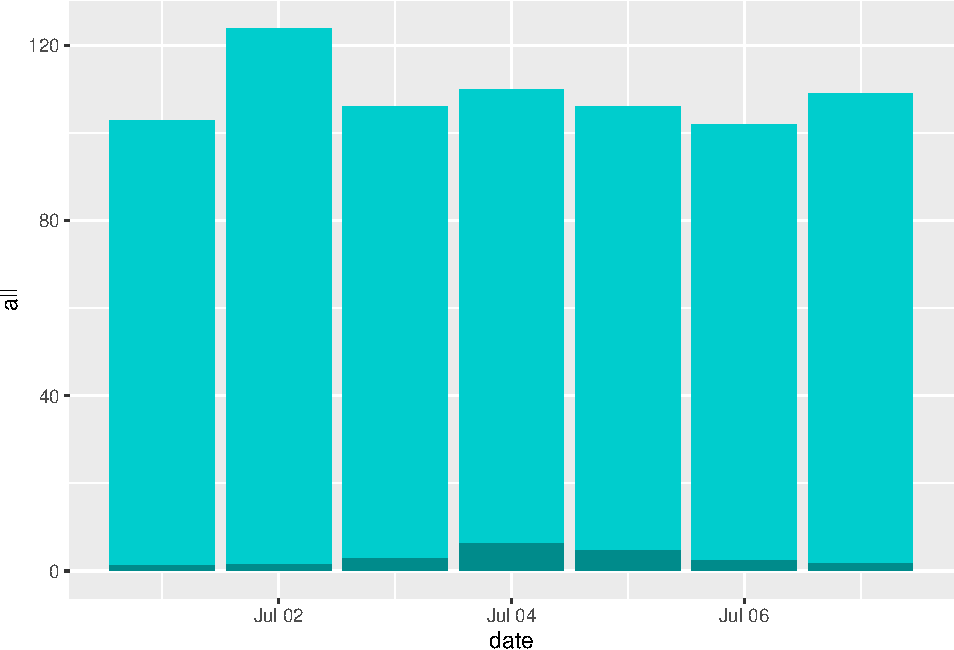
\includegraphics{adv_epi_analysis_files/figure-latex/unnamed-chunk-151-1.pdf}

With this example, you can see how you can calculate these estimates from scratch. However, this will become cumbersome as you move to larger and more complex examples. Fortunately, the authors of \citet{gasparrini2014attributable} included an R script with code for a function to do this, both for these simpler examples and as you move to more complex examples. To download the script for this function, go \href{https://raw.githubusercontent.com/gasparrini/2014_gasparrini_BMCmrm_Rcodedata/master/attrdl.R}{here} and save the file as a plain text file, with the extension ``.R''. (As a note, make sure you use this link for the file---an earlier version of the script was posted on the website of the article, but it's changed some since then, and you want the newer version.) Once you unzip this file, it should be an R script named ``attrdl.R''. Put this script somewhere convenient to your working directory and source the code in it using the \texttt{source} function. For example, if you saved the R script in a subdirectory ``code'' of the current working directory, you would run:

\begin{Shaded}
\begin{Highlighting}[]
\FunctionTok{source}\NormalTok{(}\StringTok{"code/attrdl.R"}\NormalTok{)}
\end{Highlighting}
\end{Shaded}

This will run all the code in the file, which creates a new function called \texttt{attrdl}. This function also has a helpfile, which you can find \href{https://static-content.springer.com/esm/art\%3A10.1186\%2F1471-2288-14-55/MediaObjects/12874_2014_1076_MOESM2_ESM.pdf}{here}.

The \texttt{attrdl} function has four required arguments: a vector with the exposure, a crossbasis function, a vector with the cases that correspond to each value in the exposure vector, and the value of the exposure that you want to use as a baseline. You can also include a fitted model. In our example, the exposure will be a vector of the temperature on each day of the first week of July 2012 in London, and the cases vector will be the number of deaths observed on each of those days. We will use 7 degrees C as our baseline. The crossbasis will be the crossbasis object we used to fit our model, and we'll include the fitted model. We can run the function as:

\begin{Shaded}
\begin{Highlighting}[]
\FunctionTok{attrdl}\NormalTok{(}\AttributeTok{x =}\NormalTok{ july\_week}\SpecialCharTok{$}\NormalTok{tmean, }\AttributeTok{cases =}\NormalTok{ july\_week}\SpecialCharTok{$}\NormalTok{all, }
       \AttributeTok{basis =}\NormalTok{ temp\_basis, }\AttributeTok{model =}\NormalTok{ dlnm\_mod\_1, }\AttributeTok{cen =} \DecValTok{7}\NormalTok{)}
\end{Highlighting}
\end{Shaded}

\begin{verbatim}
## [1] 0.02727977
\end{verbatim}

By default, it gives us the attributable risk for the week. You can see that this matches the value we got when we did this calculation from scratch, but it certainly saves us a lot of time. This function will also help us tackle tougher cases, like when we have model associations across a distributed lag.

You can also use this function to get the attributable number. You just need to add the argument \texttt{type\ =\ "an"}:

\begin{Shaded}
\begin{Highlighting}[]
\FunctionTok{attrdl}\NormalTok{(}\AttributeTok{x =}\NormalTok{ july\_week}\SpecialCharTok{$}\NormalTok{tmean, }\AttributeTok{cases =}\NormalTok{ july\_week}\SpecialCharTok{$}\NormalTok{all, }
       \AttributeTok{basis =}\NormalTok{ temp\_basis, }\AttributeTok{model =}\NormalTok{ dlnm\_mod\_1, }\AttributeTok{cen =} \DecValTok{7}\NormalTok{, }\AttributeTok{type =} \StringTok{"an"}\NormalTok{)}
\end{Highlighting}
\end{Shaded}

\begin{verbatim}
## [1] 20.73262
\end{verbatim}

If we want to get the values for each day of the week, we can include the argument \texttt{tot\ =\ FALSE}. This will give us an estimate for each date, rather than the estimate of the total over the period:

\begin{Shaded}
\begin{Highlighting}[]
\FunctionTok{attrdl}\NormalTok{(}\AttributeTok{x =}\NormalTok{ july\_week}\SpecialCharTok{$}\NormalTok{tmean, }\AttributeTok{cases =}\NormalTok{ july\_week}\SpecialCharTok{$}\NormalTok{all, }
       \AttributeTok{basis =}\NormalTok{ temp\_basis, }\AttributeTok{model =}\NormalTok{ dlnm\_mod\_1, }\AttributeTok{cen =} \DecValTok{7}\NormalTok{, }
       \AttributeTok{type =} \StringTok{"an"}\NormalTok{, }\AttributeTok{tot =} \ConstantTok{FALSE}\NormalTok{)}
\end{Highlighting}
\end{Shaded}

\begin{verbatim}
## [1] 1.228037 1.571579 2.855759 6.190165 4.677225 2.480511 1.729346
\end{verbatim}

Again, you can see that this agrees with the calculations we did from scratch.

\begin{enumerate}
\def\labelenumi{\arabic{enumi}.}
\setcounter{enumi}{1}
\tightlist
\item
  \textbf{Extend this idea to calculate the attributable risk and attributable number of deaths related to temperature throughout the study period. Calculate these values separately for heat and cold.}
\end{enumerate}

With the \texttt{attrdl} function, it's very straightforward to extend these calculations to look at the whole study period, rather than just one week. The only tricky part, conceptually, is that we want to generate separate estimates for heat and cold. Heat-attributable mortality will only occur when the temperature is higher than our baseline of 7 degrees Celsius, while cold-attributable mortality will only occur when the temperature is lower than 7 degrees Celsius.

One way we can do this is to split apart the original dataset into two datasets---one with all the observations on ``cold'' days (those below 7 degrees C) and one with all the observations on ``hot'' days (those above 8 degrees C). Then we can run the function to calculate attributable risk and attributable number on these two datasets separately, to get separate estimates for heat-attributable and cold attributable mortality.

\begin{Shaded}
\begin{Highlighting}[]
\NormalTok{obs\_cold }\OtherTok{\textless{}{-}}\NormalTok{ obs }\SpecialCharTok{\%\textgreater{}\%} 
  \FunctionTok{filter}\NormalTok{(tmean }\SpecialCharTok{\textless{}} \DecValTok{7}\NormalTok{)}
\NormalTok{obs\_hot }\OtherTok{\textless{}{-}}\NormalTok{ obs }\SpecialCharTok{\%\textgreater{}\%} 
  \FunctionTok{filter}\NormalTok{(tmean }\SpecialCharTok{\textgreater{}} \DecValTok{7}\NormalTok{)}

\CommentTok{\# Estimate cold{-}related attributable risk over the study period}
\FunctionTok{attrdl}\NormalTok{(}\AttributeTok{x =}\NormalTok{ obs\_cold}\SpecialCharTok{$}\NormalTok{tmean, }\AttributeTok{cases =}\NormalTok{ obs\_cold}\SpecialCharTok{$}\NormalTok{all, }
       \AttributeTok{basis =}\NormalTok{ temp\_basis, }\AttributeTok{model =}\NormalTok{ dlnm\_mod\_1, }
       \AttributeTok{cen =} \DecValTok{7}\NormalTok{)}
\end{Highlighting}
\end{Shaded}

\begin{verbatim}
## [1] 0.007327224
\end{verbatim}

\begin{Shaded}
\begin{Highlighting}[]
\CommentTok{\# Estimate cold{-}related attributable number over the study period}
\FunctionTok{attrdl}\NormalTok{(}\AttributeTok{x =}\NormalTok{ obs\_cold}\SpecialCharTok{$}\NormalTok{tmean, }\AttributeTok{cases =}\NormalTok{ obs\_cold}\SpecialCharTok{$}\NormalTok{all, }
       \AttributeTok{basis =}\NormalTok{ temp\_basis, }\AttributeTok{model =}\NormalTok{ dlnm\_mod\_1, }
       \AttributeTok{cen =} \DecValTok{7}\NormalTok{, }\AttributeTok{type =} \StringTok{"an"}\NormalTok{)}
\end{Highlighting}
\end{Shaded}

\begin{verbatim}
## [1] 2414.899
\end{verbatim}

\begin{Shaded}
\begin{Highlighting}[]
\CommentTok{\# Estimate heat{-}related attributable risk over the study period}
\FunctionTok{attrdl}\NormalTok{(}\AttributeTok{x =}\NormalTok{ obs\_hot}\SpecialCharTok{$}\NormalTok{tmean, }\AttributeTok{cases =}\NormalTok{ obs\_hot}\SpecialCharTok{$}\NormalTok{all, }
       \AttributeTok{basis =}\NormalTok{ temp\_basis, }\AttributeTok{model =}\NormalTok{ dlnm\_mod\_1, }
       \AttributeTok{cen =} \DecValTok{7}\NormalTok{)}
\end{Highlighting}
\end{Shaded}

\begin{verbatim}
## [1] 0.0235678
\end{verbatim}

\begin{Shaded}
\begin{Highlighting}[]
\CommentTok{\# Estimate cold{-}related attributable number over the study period}
\FunctionTok{attrdl}\NormalTok{(}\AttributeTok{x =}\NormalTok{ obs\_hot}\SpecialCharTok{$}\NormalTok{tmean, }\AttributeTok{cases =}\NormalTok{ obs\_hot}\SpecialCharTok{$}\NormalTok{all, }
       \AttributeTok{basis =}\NormalTok{ temp\_basis, }\AttributeTok{model =}\NormalTok{ dlnm\_mod\_1, }
       \AttributeTok{cen =} \DecValTok{7}\NormalTok{, }\AttributeTok{type =} \StringTok{"an"}\NormalTok{)}
\end{Highlighting}
\end{Shaded}

\begin{verbatim}
## [1] 23484.98
\end{verbatim}

Another way that you can do this is to use the \texttt{range} argument in \texttt{attrdl}, which allows you to focus on the impacts in only one range of the exposure. For example, you could estimate the heat-related attributable number by using a range from the baseline temperature to the maximum temperature in the observations:

\begin{Shaded}
\begin{Highlighting}[]
\FunctionTok{attrdl}\NormalTok{(}\AttributeTok{x =}\NormalTok{ obs}\SpecialCharTok{$}\NormalTok{tmean, }\AttributeTok{cases =}\NormalTok{ obs}\SpecialCharTok{$}\NormalTok{all, }
       \AttributeTok{basis =}\NormalTok{ temp\_basis, }\AttributeTok{model =}\NormalTok{ dlnm\_mod\_1, }
       \AttributeTok{cen =} \DecValTok{7}\NormalTok{, }\AttributeTok{range =} \FunctionTok{c}\NormalTok{(}\DecValTok{7}\NormalTok{, }\FunctionTok{max}\NormalTok{(obs}\SpecialCharTok{$}\NormalTok{tmean)), }\AttributeTok{type =} \StringTok{"an"}\NormalTok{)}
\end{Highlighting}
\end{Shaded}

\begin{verbatim}
## [1] 23484.98
\end{verbatim}

Based on these estimates, there were about 23,500 deaths over the approximately two-decade study period in London that we would expect to not have occurred if the temperature never exceeded 7 degrees C. This makes up about 2\% of all mortality on days above 7 degrees C. On the other hand, based on this assessment, the impact from cold is much lower---only about 2,500 attributable deaths over the approximately two-decade study period, making only about 0.7\% of all the deaths on days colder than 7 degrees C.

There are a few caveats with these estimates. First, there are a lot fewer days that were below 7 degrees C in the study than that were above. This accounts for some of the difference in the total number of excess deaths attributable to heat versus cold over the study period. The location of the minimum mortality temperature, which we estimated from fitting a model with only immediate effects in this case, might shift as we include more lags, in which case we would recenter our estimates of attributable risk and attributable number in terms of the baseline temperature we compare to. This could change the numbers some just from having more days above or below the threshold.

Second, we know from fitting the distributed lag non-linear models in an earlier chapter that cold tends to have a more lagged effect on mortality risk, while the effect of heat is more immediate. By limiting the model to lag 0, we've likely missed a lot of the effect of cold on mortality risk. We'll address this in the next part of the exercise, where we'll expand to use a model with a distributed lag.

Finally, the choice of a baseline is tricky here. We're using the minimum mortality temperature, and that's a common choice. However, it's pretty unrealistic to think that there would be a way that this ``safest'' baseline scenario would ever be met---you'd never be able to enforce the temperature in a city staying constant year-round. Another approach could be to take a sample ``mild'' summer and ``mild'' winter for your study city, and compare the health impacts during more severe years to that milder case. This would require a bit more work to calculate, as your baseline temperature would be changing throughout each season. There's not a perfect solution to this issue of identifying a baseline, but it's important to be clear when you communicate the baseline you're using when you describe your results.

Going back to the \texttt{attrdl} function, you can use the \texttt{tot\ =\ FALSE} argument to check out some interesting patterns in attributable numbers over your study. This argument estimates the attributable risk or number for each separate day in the study. For example, you can use it to add a column to your original data with the estimated attributable number for that day:

\begin{Shaded}
\begin{Highlighting}[]
\NormalTok{obs\_an\_added }\OtherTok{\textless{}{-}}\NormalTok{ obs }\SpecialCharTok{\%\textgreater{}\%} 
  \FunctionTok{select}\NormalTok{(date, tmean, all) }\SpecialCharTok{\%\textgreater{}\%} 
  \FunctionTok{mutate}\NormalTok{(}\AttributeTok{an =} \FunctionTok{attrdl}\NormalTok{(}\AttributeTok{x =}\NormalTok{ obs}\SpecialCharTok{$}\NormalTok{tmean, }\AttributeTok{cases =}\NormalTok{ obs}\SpecialCharTok{$}\NormalTok{all, }
                     \AttributeTok{basis =}\NormalTok{ temp\_basis, }\AttributeTok{model =}\NormalTok{ dlnm\_mod\_1, }
                     \AttributeTok{cen =} \DecValTok{7}\NormalTok{, }\AttributeTok{type =} \StringTok{"an"}\NormalTok{, }\AttributeTok{tot =} \ConstantTok{FALSE}\NormalTok{))}
\NormalTok{obs\_an\_added}
\end{Highlighting}
\end{Shaded}

\begin{verbatim}
## # A tibble: 8,279 x 4
##    date       tmean   all      an
##    <date>     <dbl> <dbl>   <dbl>
##  1 1990-01-01  3.91   220  1.09  
##  2 1990-01-02  5.55   257  0.0294
##  3 1990-01-03  4.39   245  0.756 
##  4 1990-01-04  5.43   226  0.0685
##  5 1990-01-05  6.87   236 -0.0395
##  6 1990-01-06  9.23   235  1.74  
##  7 1990-01-07  6.69   231 -0.0780
##  8 1990-01-08  7.96   235  0.546 
##  9 1990-01-09  7.27   250  0.114 
## 10 1990-01-10  9.51   214  1.84  
## # i 8,269 more rows
\end{verbatim}

With this, we can look at how the number of excess deaths vary by temperature. We can bin temperatures into broad bins and then plot the total number of attributable deaths for days with each temperature:

\begin{Shaded}
\begin{Highlighting}[]
\NormalTok{obs\_an\_added }\SpecialCharTok{\%\textgreater{}\%} 
  \FunctionTok{mutate}\NormalTok{(}\AttributeTok{temp\_round =} \FunctionTok{round}\NormalTok{(tmean)) }\SpecialCharTok{\%\textgreater{}\%} 
  \FunctionTok{group\_by}\NormalTok{(temp\_round) }\SpecialCharTok{\%\textgreater{}\%} 
  \FunctionTok{summarize}\NormalTok{(}\AttributeTok{an\_tot =} \FunctionTok{sum}\NormalTok{(an)) }\SpecialCharTok{\%\textgreater{}\%} 
  \FunctionTok{ggplot}\NormalTok{(}\FunctionTok{aes}\NormalTok{(}\AttributeTok{x =}\NormalTok{ temp\_round, }\AttributeTok{y =}\NormalTok{ an\_tot)) }\SpecialCharTok{+} 
  \FunctionTok{geom\_col}\NormalTok{() }\SpecialCharTok{+} 
  \FunctionTok{labs}\NormalTok{(}\AttributeTok{x =} \StringTok{"Mean daily temperature"}\NormalTok{, }
       \AttributeTok{y =} \StringTok{"Total attributable excess deaths on}\SpecialCharTok{\textbackslash{}n}\StringTok{days with that temperature"}\NormalTok{)}
\end{Highlighting}
\end{Shaded}

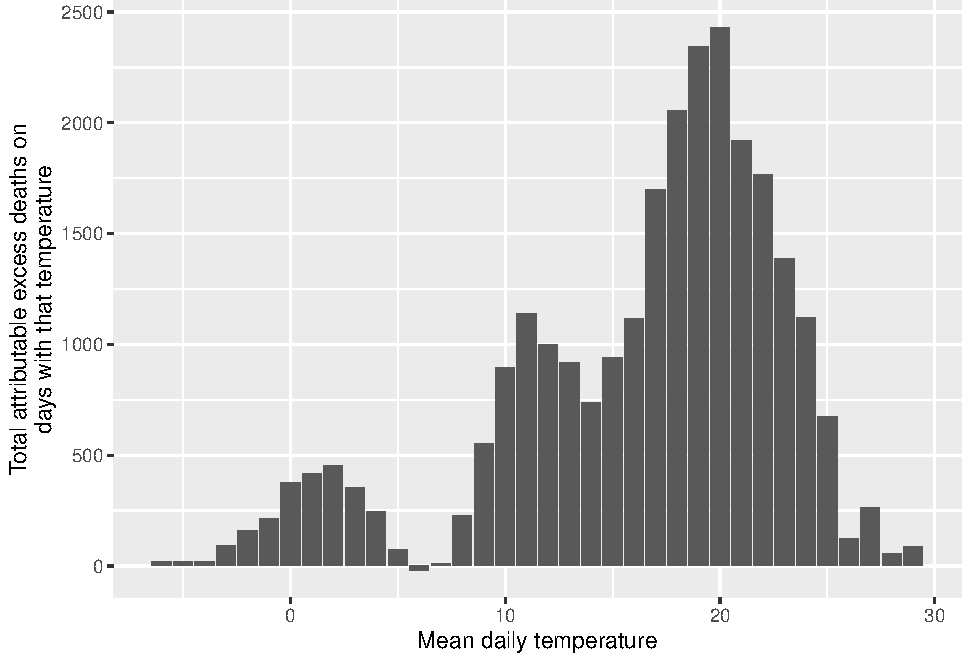
\includegraphics{adv_epi_analysis_files/figure-latex/unnamed-chunk-159-1.pdf}

Remember that our exposure-response function increased dramatically at extreme temperatures, especially extreme heat. Here, however, we see the role that frequency of exposure plays in the ultimate impact. Because extremely hot and extremely cold days are very rare, they don't account for much of the heat- or cold-attributable mortality. Instead, a lot more comes at temperatures that are a bit milder than those extremes but that occur much more often. This, of course, might change depending on the baseline we're using for comparison.

\begin{enumerate}
\def\labelenumi{\arabic{enumi}.}
\setcounter{enumi}{2}
\tightlist
\item
  \textbf{Do the same calculation as in the previous part, but change the underlying model that you're using. In this case, use the \texttt{dist\_lag\_mod\_5} you fit in Chapter 4. What differences are there in attributable risk and attributable number when you use a model that incorporates lagged effects (\texttt{dist\_lag\_mod\_5}) compared to one that only fits the immediate association (\texttt{dlnm\_mod\_1})?}
\end{enumerate}

To start, re-run the code we used in Chapter 4 to fit \texttt{dist\_lag\_mod\_5}, including the code to create the associated crossbasis function (\texttt{dl\_basis\_4}):

\begin{Shaded}
\begin{Highlighting}[]
\NormalTok{dl\_basis\_4 }\OtherTok{\textless{}{-}} \FunctionTok{crossbasis}\NormalTok{(obs}\SpecialCharTok{$}\NormalTok{tmean, }\AttributeTok{lag =} \DecValTok{30}\NormalTok{,}
                       \AttributeTok{argvar =} \FunctionTok{list}\NormalTok{(}\AttributeTok{fun =} \StringTok{"ns"}\NormalTok{, }\AttributeTok{df =} \DecValTok{4}\NormalTok{), }
                       \AttributeTok{arglag =} \FunctionTok{list}\NormalTok{(}\AttributeTok{fun =} \StringTok{"ns"}\NormalTok{, }\AttributeTok{df =} \DecValTok{6}\NormalTok{))}
\NormalTok{dist\_lag\_mod\_5 }\OtherTok{\textless{}{-}} \FunctionTok{glm}\NormalTok{(all }\SpecialCharTok{\textasciitilde{}}\NormalTok{ dl\_basis\_4 }\SpecialCharTok{+} 
                        \FunctionTok{factor}\NormalTok{(dow, }\AttributeTok{ordered =} \ConstantTok{FALSE}\NormalTok{) }\SpecialCharTok{+}
                          \FunctionTok{ns}\NormalTok{(time, }\AttributeTok{df =} \DecValTok{158}\NormalTok{), }
                        \AttributeTok{data =}\NormalTok{ obs, }\AttributeTok{family =} \StringTok{"quasipoisson"}\NormalTok{)}
\end{Highlighting}
\end{Shaded}

First, let's take a look to see if we should use a different baseline---in other words, is 7 degrees C still our best estimate of the minimum mortality temperature, now that we're incorporating lagged effects? If we use \texttt{crosspred}, we can check the exposure-response curve for the cumulative effects over all the fitted lags, to see what the minimum point is on that curve:

\begin{Shaded}
\begin{Highlighting}[]
\FunctionTok{crosspred}\NormalTok{(dl\_basis\_4, dist\_lag\_mod\_5, }\AttributeTok{bylag =} \DecValTok{1}\NormalTok{) }\SpecialCharTok{\%\textgreater{}\%} 
  \FunctionTok{plot}\NormalTok{(}\AttributeTok{ptype =} \StringTok{"overall"}\NormalTok{)}
\end{Highlighting}
\end{Shaded}

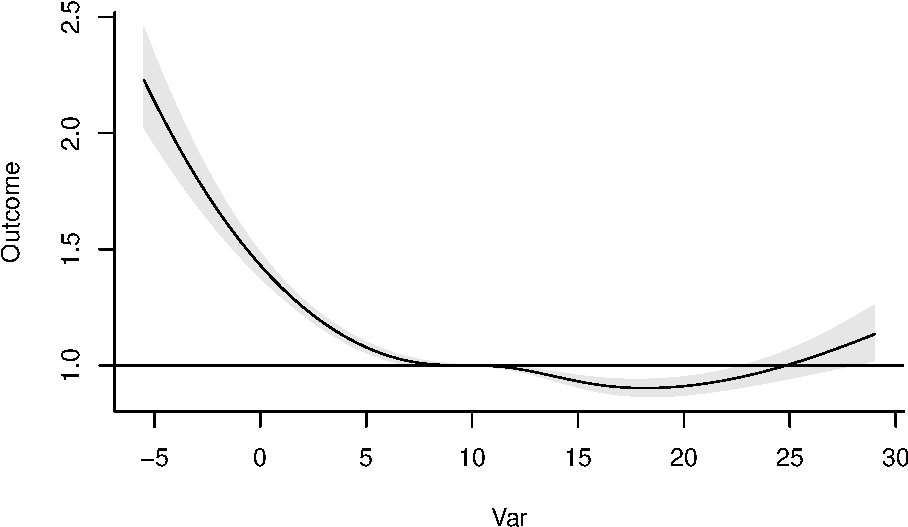
\includegraphics{adv_epi_analysis_files/figure-latex/unnamed-chunk-161-1.pdf}

Now that we're considering lagged effects, the temperature with minimum mortality risk has gone up quite a lot, to 18 degrees C. We'll use that as our baseline in estimating attributable risk and number for heat and cold. We can already tell that this will increase our cold-attributable mortality by a bit most likely, since there will be a lot more days that are below this baseline temperature now. Following the same reasoning, this is also likely to decrease the heat-attributable mortality (although of course changes to the shape of the exposure-response curve will also affect our estimates).

The other thing that we need to think about is how to incorporate lagged effects of temperature. You can do this by thinking of temperatures at different lags as different exposures. The mathematics for this gets more complicated, but fortunately the \texttt{attrdl} function can handle those mechanics for us.

We do, however, have to decide whether we want to calculate these attributable impacts from lagged exposures under what's called a ``backward perspective'' or a ``forward perspective''. One of the required readings for this week has a full discussion of these two perspectives and the implications and assumptions of each \citep{gasparrini2014attributable}. Simply put, the forward perspective is describing how one day's temperature has impacts on its same day as well as following days, while the backward perspective calculates the impact that all the exposures in the lagged period before a certain day impact risk on that day.

There is a way to calculate the separate impacts of heat and cold under either of these perspectives, but the forward perspective can be prone to some bias \citep{gasparrini2014attributable}, so we'll use the backward perspective. Since we want to get estimates for heat and cold separately, we'll use the \texttt{range} argument in the \texttt{attrdl} function. (With the lagged effects, it would be tricky to try to do this by separating the dataset into hot and cold days, since you'll have some cases when you have temperatures that are both below and above the baseline temperature in the lag period.) You can specify that you'd like to use the backward perspective with the argument \texttt{dir\ =\ "back"}:

\begin{Shaded}
\begin{Highlighting}[]
\CommentTok{\# Estimate cold{-}associated attributable risk}
\FunctionTok{attrdl}\NormalTok{(}\AttributeTok{x =}\NormalTok{ obs}\SpecialCharTok{$}\NormalTok{tmean, }\AttributeTok{cases =}\NormalTok{ obs}\SpecialCharTok{$}\NormalTok{all, }
       \AttributeTok{basis =}\NormalTok{ dl\_basis\_4, }\AttributeTok{model =}\NormalTok{ dist\_lag\_mod\_5, }
       \AttributeTok{cen =} \DecValTok{18}\NormalTok{, }\AttributeTok{range =} \FunctionTok{c}\NormalTok{(}\FunctionTok{min}\NormalTok{(obs}\SpecialCharTok{$}\NormalTok{tmean), }\DecValTok{18}\NormalTok{), }\AttributeTok{dir =} \StringTok{"back"}\NormalTok{)}
\end{Highlighting}
\end{Shaded}

\begin{verbatim}
## [1] 0.09398662
\end{verbatim}

\begin{Shaded}
\begin{Highlighting}[]
\CommentTok{\# Estimate cold{-}associated attributable number}
\FunctionTok{attrdl}\NormalTok{(}\AttributeTok{x =}\NormalTok{ obs}\SpecialCharTok{$}\NormalTok{tmean, }\AttributeTok{cases =}\NormalTok{ obs}\SpecialCharTok{$}\NormalTok{all, }
       \AttributeTok{basis =}\NormalTok{ dl\_basis\_4, }\AttributeTok{model =}\NormalTok{ dist\_lag\_mod\_5, }
       \AttributeTok{cen =} \DecValTok{18}\NormalTok{, }\AttributeTok{range =} \FunctionTok{c}\NormalTok{(}\FunctionTok{min}\NormalTok{(obs}\SpecialCharTok{$}\NormalTok{tmean), }\DecValTok{18}\NormalTok{), }\AttributeTok{dir =} \StringTok{"back"}\NormalTok{, }\AttributeTok{type =} \StringTok{"an"}\NormalTok{)}
\end{Highlighting}
\end{Shaded}

\begin{verbatim}
## [1] 124632.4
\end{verbatim}

\begin{Shaded}
\begin{Highlighting}[]
\CommentTok{\# Estimate heat{-}associated attributable risk}
\FunctionTok{attrdl}\NormalTok{(}\AttributeTok{x =}\NormalTok{ obs}\SpecialCharTok{$}\NormalTok{tmean, }\AttributeTok{cases =}\NormalTok{ obs}\SpecialCharTok{$}\NormalTok{all, }
       \AttributeTok{basis =}\NormalTok{ dl\_basis\_4, }\AttributeTok{model =}\NormalTok{ dist\_lag\_mod\_5, }
       \AttributeTok{cen =} \DecValTok{18}\NormalTok{, }\AttributeTok{range =} \FunctionTok{c}\NormalTok{(}\DecValTok{18}\NormalTok{, }\FunctionTok{max}\NormalTok{(obs}\SpecialCharTok{$}\NormalTok{tmean)), }\AttributeTok{dir =} \StringTok{"back"}\NormalTok{)}
\end{Highlighting}
\end{Shaded}

\begin{verbatim}
## [1] 0.002380825
\end{verbatim}

\begin{Shaded}
\begin{Highlighting}[]
\CommentTok{\# Estimate heat{-}associated attributable number}
\FunctionTok{attrdl}\NormalTok{(}\AttributeTok{x =}\NormalTok{ obs}\SpecialCharTok{$}\NormalTok{tmean, }\AttributeTok{cases =}\NormalTok{ obs}\SpecialCharTok{$}\NormalTok{all, }
       \AttributeTok{basis =}\NormalTok{ dl\_basis\_4, }\AttributeTok{model =}\NormalTok{ dist\_lag\_mod\_5, }
       \AttributeTok{cen =} \DecValTok{18}\NormalTok{, }\AttributeTok{range =} \FunctionTok{c}\NormalTok{(}\DecValTok{18}\NormalTok{, }\FunctionTok{max}\NormalTok{(obs}\SpecialCharTok{$}\NormalTok{tmean)), }\AttributeTok{dir =} \StringTok{"back"}\NormalTok{, }\AttributeTok{type =} \StringTok{"an"}\NormalTok{)}
\end{Highlighting}
\end{Shaded}

\begin{verbatim}
## [1] 3157.129
\end{verbatim}

When we use this model that includes distributed lag effects of temperature, you can see that the impact of cold has increased substantially and the impact of heat has decreased substantially. This is because cold tends to have effects that are lagged after the initial exposure, while heat tends to be more immediate, and can even have somewhat of a pattern reflective of mortality displacement (although this depends on the study city). Once we incorporate the delayed effects of cold, the minimum mortality temperature also increase substantially, so many more days are below, rather than above, the baseline temperature we're using for comparison as compared to the last part of the exercise.

These long lagged effects of temperature start to bring in some questions about whether the effect is specifically from the absolute value of the temperature, or whether they may be starting to pick up some impacts that are caused by seasonality, rather than absolute temperature. As you include lags up to a month or longer, it gets harder to separate the impact of temperature specifically from the impact of season. This question is very important when you start thinking about the impacts of climate change. With climate change, we expect in many places that winter days will, on average, have a higher temperature. If the mortality risk of cold is caused by the absolute temperature, this would result in fewer cold-related deaths. However, if there are other seasonal factors (that we don't expect to change, or at least not as much), then the rising winter temperatures would have less of a beneficial effect on winter mortality risk. There are a number of interesting papers that focus on this question and its implications for climate change projections \citep{kinney2015winter, ebi2015greater, hajat2016excess}. Also, there are some papers that go more deeply into how to estimate minimum mortality temperatures \citep{lee2017monte, tobias2017investigating}, as well as what baseline temperature makes a suitable threshold for estimating attributable risk for cold-related mortality \citep{arbuthnott2018cold}.

\section{Quantifying potential health impacts under different scenarios}\label{quantifying-potential-health-impacts-under-different-scenarios}

You can use measures of attributable risk and attributable number to communicate the estimated impacts of the exposure in the population that you studied. However, you can also use this same idea to investigate the potential health impacts of an exposure under different scenarios. The basic framework on these calculations was to compare one scenario (a baseline of no, limited, or ``safest'' exposure) to another scenario (the observed levels of exposure in the population). It's fairly straightforward to transfer this idea to broader applications---any case where you would like to compare one scenario of exposure to another scenario of exposure.

You could do this a few ways. One is that you could calculate attributable impacts under both scenarios in comparison to some baseline, and compare the final impact estimates. One of this week's readings \citep{vicedo2019hands} describes this process, adding a code tutorial in the supplement. It describes the process in the context of projecting the potential heat-related mortality impacts of climate change, compared to present-day impacts.

There are a few details that make this process a bit different from calculating attributable impacts based on the study data you used to fit the model. First, you do not have observations of exposure. Instead, you will use scenarios of exposure, generated under certain assumptions. For climate change projections, there are large climate modeling groups that have generated scenarios of future weather conditions under scenarios that are tied to assumptions about how drivers of climate change will change in the future. These scenarios can be used in place of exposure observations to project potential health impacts. Of course, there are more uncertainties that are introduced in this case, compared to observed exposures, since there is some uncertainty in those projections. Further, it is typically best to work with atmospheric scientists in deriving exposure scenarios from these projections, as you'll need expertise to appropriately convert the climate model output to an appropriate representation of temperature exposures in a future period.

Second, you will not have the observed number of cases (for example, deaths) on each day of a hypothetical scenario. Instead, you will need to incorporate an estimate of mortality each day in the scenario. One approach is to use present-day average daily mortality counts, as this allows you to isolate the role of climate change, separate from changes in demographics. Further, if you are considering scenarios that happen in the near future, this is a very reasonable approach. However, if you're considering scenarios a few decades in the future, this won't give a good estimate of the impact we might actually expect. One approach to try to improve this estimate is to use demographic projections of population into the future. You can pair this with mortality rates in certain subsets of the population (these could be, for example, by age and race) to try to generate a more realistic estimate of future impacts.

Finally, when you use the estimate exposure-response functions that are estimated with present-day data to project impacts in a future period, there are a number of reasons that the exposure-response function might not provide as good of an estimate of how temperature would impact health. Exposure-response functions for temperature are not the same in every city. Instead, there's clear evidence that, in cities with cooler climates, heat tends to start affecting risk at a lower temperature, and, in cities with hotter climates, cold tends to start affecting risk at a higher temperature. In other words, there's not an ``absolute'' shape, tied to specific temperature values, that can universally describe how mortality risk changes with temperature. Further, there is evidence that these exposure-response functions have changed in the same city over time. This all suggests that there's likely some influence from adaptation on these exposure-response functions. For example, a decreasing risk from heat over the 20th century likely was, at least in part, caused by adaptation through the invention and increased use of air conditioning, which reduces exposure to heat for at least some of the population at least some of the time. Other changes can come from changes in the population structure. For example, we know that temperature-related risk tends to be higher in older versus younger adults, so if a population is aging, that could change the shape of its overall exposure-response function, even without other changes. These questions are an area of continuing development for climate epidemiologists. Good discussions are available in a number of papers, including \citet{kinney2008approaches}, \citet{arbuthnott2016changes}, \citet{gosling2017adaptation}, and \citet{kinney2018temporal}.

\chapter{Longitudinal cohort study designs}\label{longitudinal-cohort-study-designs}

\section{Readings}\label{readings-4}

The required readings for this chapter are:

\begin{itemize}
\item
  \citet{andersson201970} Provides background on the study we'll use in this chapter for our example data
\item
  \citet{wong1989risk} An epidemiological study using the study data.
\end{itemize}

There are also some supplemental readings you may find useful. The following are a series of instructional papers on survival analysis, that are
meant as general background on how to fit survival analysis models:

\begin{itemize}
\item
  \citet{clark2003survival}
\item
  \citet{bradburn2003survival}
\item
  \citet{bradburn2003survival2}
\end{itemize}

This article is a good summary for the limitations of Hazards Ratios and offers an alternative survival analysis approach enabling the plotting of adjusted cumulative incidence (and similarly survival rate) curves:

\begin{itemize}
\tightlist
\item
  \citet{hernan2010hazards} (Note that there is an online erratum for this article: ``On page 15, column 1, second full paragraph: `\ldots{} and the average HR is ensured to reach the value 1.' should instead say, `\ldots{} and the risk ratio is ensured to reach the value 1.'\,'')
\end{itemize}

These articles provide more background on the Framingham Heart Study:

\begin{itemize}
\tightlist
\item
  \citet{dawber1951epidemiological} A paper from the 1950s, this presents the rationale behind the design of the Framingham Heart Study
\item
  \citet{dawber2015ii} A reprint of the paper describing the first results to come out of the Framingham Heart Study
\end{itemize}

These articles provide some general reviews on our current understanding of the epidemiology and etiology of heart disease and its risk factors:

\begin{itemize}
\tightlist
\item
  \citet{wong2014epidemiological} Review of large epidemiological studies on coronary heart disease and key findings
\item
  \citet{ziaeian2016epidemiology} Review on the epidemiology and etiology of heart failure
\item
  \citet{valenzuela2021lifestyle} Review of risk factors for hypertension
\item
  \citet{zhou2021global} Review on global epidemiology of hypertension
\end{itemize}

\section{Longitudinal cohort data}\label{longitudinal-cohort-data}

Our example data for this chapter comes from the Framingham Heart Study. This is a cohort study that began in 1948 \citep{andersson201970}. At the time (and continuing today), heart disease was the most common cause of death in the US---a notable shift from earlier times, when infectious diseases played a larger role in mortality. While heart disease was an important cause of death, however, very little was known about risk factors for heart disease, outside of a little concerning the role of some infectious and nutritional diseases that affected the heart \citep{dawber1951epidemiological, andersson201970}. This study was designed to collect a group of people without evident cardiovascular disease (although this restriction was eased in practice) and track them over many years, to try to identify risk factors for developing cardiovascular disease. The study subjects were tracked over time, with data regularly collected on both risk factors and cardiovascular outcomes. The study was revolutionary in identifying some key risk factors for coronary heart disease, including elevated blood pressure, high cholesterol levels, being overweight, and smoking \citep{andersson201970}. It was also revolutionary in identifying high blood pressure as a risk for other cardiovascular outcomes, including stroke and congestive heart failure \citep{andersson201970}.

The original cohort included about 5,200 people from the town of Framingham, MA. The
example data is a subset of data from this original cohort. You can download the example dataset for this class by clicking \href{https://github.com/geanders/adv_epi_analysis/raw/master/data/frmgham2.csv}{here} and then saving the content of the page as a csv file (we recommend using the original filename of ``frmgham2.csv''). There is also a codebook file that comes with these data, which you can download for this class by clicking \href{https://github.com/geanders/adv_epi_analysis/raw/master/data/Framingham\%20Longitudinal\%20Data\%20Documentation.pdf}{here}. This codebook includes some explanations about the columns in the data, as well as how multiple measurements from a single study subject are included in the data.

The data are saved in a csv format, and so they can be read into R using the
\texttt{read\_csv} function from the \texttt{readr} package (part of the tidyverse). You can use the following code to read in these data, assuming you have saved them in a ``data'' subdirectory of your current
working directory:

\begin{Shaded}
\begin{Highlighting}[]
\FunctionTok{library}\NormalTok{(tidyverse) }\CommentTok{\# Loads all the tidyverse packages, including readr}
\NormalTok{fhs }\OtherTok{\textless{}{-}} \FunctionTok{read\_csv}\NormalTok{(}\StringTok{"data/frmgham2.csv"}\NormalTok{)}
\NormalTok{fhs}
\end{Highlighting}
\end{Shaded}

\begin{verbatim}
## # A tibble: 11,627 x 39
##    RANDID   SEX TOTCHOL   AGE SYSBP DIABP CURSMOKE CIGPDAY   BMI DIABETES BPMEDS
##     <dbl> <dbl>   <dbl> <dbl> <dbl> <dbl>    <dbl>   <dbl> <dbl>    <dbl>  <dbl>
##  1   2448     1     195    39  106   70          0       0  27.0        0      0
##  2   2448     1     209    52  121   66          0       0  NA          0      0
##  3   6238     2     250    46  121   81          0       0  28.7        0      0
##  4   6238     2     260    52  105   69.5        0       0  29.4        0      0
##  5   6238     2     237    58  108   66          0       0  28.5        0      0
##  6   9428     1     245    48  128.  80          1      20  25.3        0      0
##  7   9428     1     283    54  141   89          1      30  25.3        0      0
##  8  10552     2     225    61  150   95          1      30  28.6        0      0
##  9  10552     2     232    67  183  109          1      20  30.2        0      0
## 10  11252     2     285    46  130   84          1      23  23.1        0      0
## # i 11,617 more rows
## # i 28 more variables: HEARTRTE <dbl>, GLUCOSE <dbl>, educ <dbl>,
## #   PREVCHD <dbl>, PREVAP <dbl>, PREVMI <dbl>, PREVSTRK <dbl>, PREVHYP <dbl>,
## #   TIME <dbl>, PERIOD <dbl>, HDLC <dbl>, LDLC <dbl>, DEATH <dbl>,
## #   ANGINA <dbl>, HOSPMI <dbl>, MI_FCHD <dbl>, ANYCHD <dbl>, STROKE <dbl>,
## #   CVD <dbl>, HYPERTEN <dbl>, TIMEAP <dbl>, TIMEMI <dbl>, TIMEMIFC <dbl>,
## #   TIMECHD <dbl>, TIMESTRK <dbl>, TIMECVD <dbl>, TIMEDTH <dbl>, ...
\end{verbatim}

You can find full details on the structure of this data in the codebook. At a broad scale, note that it includes several health outcomes related to heart disease, which the codebook calls ``events'' (\texttt{DEATH}: indicator of death from any cause; \texttt{ANYCHD}: indicator of one of several types of events related to coronary heart disease; \texttt{HOSPMI}: Hopitalization for myocardial infarction {[}heart attack{]}, etc.). The data also includes a number of risk factors that the study researchers hypothesized might be linked to cardiovascular disease (\texttt{CURSMOKE}: if the study subject is currently a smoker; \texttt{TOTCHOL}: serum total cholesterol; \texttt{SYSBP}, \texttt{DIABP}: measures of the systolic and diastolic blood pressure, respectively; \texttt{BMI}: Body Mass Index; etc.). Finally, there are some characteristics of the study subject, like age (\texttt{AGE}) and sex (\texttt{SEX}), as well as some variables that are connected to either the time of the record or the time of certain events (or of censoring, if the event did not happen during follow-up).

As you look through the data, pay attention to some features that are more characteristic of cohort studies, compared to features of the time series data we worked with in earlier chapters:

\begin{itemize}
\tightlist
\item
  One important difference compared to a time-series dataset is the \texttt{RANDID} variable. This is the unique identifier for unit for which we have repeated observations for over time.
  In this case the \texttt{RANDID} variable represents a unique identifier for each study participant, with multiple observations (rows) per participant over time.
\item
  The \texttt{TIME} variable indicates the number of days that have elapsed since beginning of follow-up of each observation. \texttt{TIME} is always 0 for the first observation of each participant (when \texttt{PERIOD} equals 1, for the first examination), and then for following measurements will track the time since follow-up started for that study participant.
\item
  The number of observations varies between participants (typical of many cohort studies)
\item
  The time spacing between observations is not constant. This is because the repeated observations in the Framingham Heart Study are the result of follow-up exams happening 3 to 5 years apart. Many longitudinal cohorts will instead have observations over a fixed time interval (monthly, annual, biannual etc), resulting in a more balanced dataset.
\item
  Observations are given for various risk factors, covariates and cardiovascular outcomes. Some will be invariant for each participant over time (\texttt{SEX}, \texttt{educ}), while others will vary with each exam.
\end{itemize}

From a data management perspective, we might want to change all the column names
to be in lowercase, rather than uppercase. This will save our pinkies some
work as we code with the data! You can make that change with the following
code, using the \texttt{str\_to\_lower} function from the \texttt{stringr} package (part of
the \texttt{tidyverse}):

\begin{Shaded}
\begin{Highlighting}[]
\NormalTok{fhs }\OtherTok{\textless{}{-}}\NormalTok{ fhs }\SpecialCharTok{\%\textgreater{}\%} 
  \FunctionTok{rename\_all}\NormalTok{(}\AttributeTok{.funs =}\NormalTok{ str\_to\_lower)}
\NormalTok{fhs}
\end{Highlighting}
\end{Shaded}

\begin{verbatim}
## # A tibble: 11,627 x 39
##    randid   sex totchol   age sysbp diabp cursmoke cigpday   bmi diabetes bpmeds
##     <dbl> <dbl>   <dbl> <dbl> <dbl> <dbl>    <dbl>   <dbl> <dbl>    <dbl>  <dbl>
##  1   2448     1     195    39  106   70          0       0  27.0        0      0
##  2   2448     1     209    52  121   66          0       0  NA          0      0
##  3   6238     2     250    46  121   81          0       0  28.7        0      0
##  4   6238     2     260    52  105   69.5        0       0  29.4        0      0
##  5   6238     2     237    58  108   66          0       0  28.5        0      0
##  6   9428     1     245    48  128.  80          1      20  25.3        0      0
##  7   9428     1     283    54  141   89          1      30  25.3        0      0
##  8  10552     2     225    61  150   95          1      30  28.6        0      0
##  9  10552     2     232    67  183  109          1      20  30.2        0      0
## 10  11252     2     285    46  130   84          1      23  23.1        0      0
## # i 11,617 more rows
## # i 28 more variables: heartrte <dbl>, glucose <dbl>, educ <dbl>,
## #   prevchd <dbl>, prevap <dbl>, prevmi <dbl>, prevstrk <dbl>, prevhyp <dbl>,
## #   time <dbl>, period <dbl>, hdlc <dbl>, ldlc <dbl>, death <dbl>,
## #   angina <dbl>, hospmi <dbl>, mi_fchd <dbl>, anychd <dbl>, stroke <dbl>,
## #   cvd <dbl>, hyperten <dbl>, timeap <dbl>, timemi <dbl>, timemifc <dbl>,
## #   timechd <dbl>, timestrk <dbl>, timecvd <dbl>, timedth <dbl>, ...
\end{verbatim}

To look a bit more closely at how this dataset works, let's take a look just at the observations of the oldest study subjects at the first examination, those 69 or older (\texttt{age\ \textgreater{}=\ 69}) at their first examination (\texttt{period\ ==\ 1}):

\begin{Shaded}
\begin{Highlighting}[]
\NormalTok{oldest\_subjects }\OtherTok{\textless{}{-}}\NormalTok{ fhs }\SpecialCharTok{\%\textgreater{}\%} 
  \FunctionTok{filter}\NormalTok{(period }\SpecialCharTok{==} \DecValTok{1} \SpecialCharTok{\&}\NormalTok{ age }\SpecialCharTok{\textgreater{}=} \DecValTok{69}\NormalTok{) }\SpecialCharTok{\%\textgreater{}\%} 
  \FunctionTok{pull}\NormalTok{(randid)}
\NormalTok{oldest\_subjects}
\end{Highlighting}
\end{Shaded}

\begin{verbatim}
##  [1] 3603542 3762702 4726021 7198139 7351212 7568367 7659676 7695005 8723664
## [10] 9643995 9686180 9789948
\end{verbatim}

Once we have the IDs of these study subjects (\texttt{oldest\_subjects}), we can pull out the study data just for them. I'm limiting to a few columns: their ID (\texttt{randid}), the time of each examination (\texttt{time}), the number of each examination (\texttt{period}), whether they died during follow-up (\texttt{died}), and the number of days between the first examination and either death (if they died during follow-up) or censoring (i.e., stopped tracking the subject or lost them to follow-up) (\texttt{timedth}):

\begin{Shaded}
\begin{Highlighting}[]
\NormalTok{fhs }\SpecialCharTok{\%\textgreater{}\%} 
  \FunctionTok{filter}\NormalTok{(randid }\SpecialCharTok{\%in\%}\NormalTok{ oldest\_subjects) }\SpecialCharTok{\%\textgreater{}\%} 
  \FunctionTok{select}\NormalTok{(randid, time, period, death, timedth)}
\end{Highlighting}
\end{Shaded}

\begin{verbatim}
## # A tibble: 24 x 5
##     randid  time period death timedth
##      <dbl> <dbl>  <dbl> <dbl>   <dbl>
##  1 3603542     0      1     1    1825
##  2 3762702     0      1     1    3076
##  3 3762702  2253      2     1    3076
##  4 4726021     0      1     1    4275
##  5 4726021  2134      2     1    4275
##  6 7198139     0      1     1    5384
##  7 7351212     0      1     1    4396
##  8 7351212  2146      2     1    4396
##  9 7351212  4283      3     1    4396
## 10 7568367     0      1     1    1563
## # i 14 more rows
\end{verbatim}

We can explore this subset of the data by plotting, for each of these study subjects, the timing of each of their examination periods, whether they died during follow-up, and the timing of their death or censoring:

\begin{Shaded}
\begin{Highlighting}[]
\NormalTok{fhs }\SpecialCharTok{\%\textgreater{}\%} 
  \FunctionTok{filter}\NormalTok{(randid }\SpecialCharTok{\%in\%}\NormalTok{ oldest\_subjects) }\SpecialCharTok{\%\textgreater{}\%} 
  \FunctionTok{select}\NormalTok{(randid, time, period, death, timedth) }\SpecialCharTok{\%\textgreater{}\%} 
  \FunctionTok{mutate}\NormalTok{(}\AttributeTok{randid =} \FunctionTok{as\_factor}\NormalTok{(randid), }
         \AttributeTok{randid =} \FunctionTok{fct\_reorder}\NormalTok{(randid, timedth),  }\CommentTok{\# Arrange by time to death}
         \AttributeTok{period =} \FunctionTok{as\_factor}\NormalTok{(period),}
         \AttributeTok{death =} \FunctionTok{as\_factor}\NormalTok{(death),}
         \AttributeTok{timey =}\NormalTok{ time }\SpecialCharTok{/} \FloatTok{365.25}\NormalTok{,                  }\CommentTok{\# Convert from days to years}
         \AttributeTok{timedthy =}\NormalTok{ timedth }\SpecialCharTok{/} \FloatTok{365.25}\NormalTok{) }\SpecialCharTok{\%\textgreater{}\%} 
  \FunctionTok{ggplot}\NormalTok{() }\SpecialCharTok{+} 
  \FunctionTok{geom\_segment}\NormalTok{(}\FunctionTok{aes}\NormalTok{(}\AttributeTok{x =} \DecValTok{0}\NormalTok{, }\AttributeTok{xend =}\NormalTok{ timedthy, }
                   \AttributeTok{y =}\NormalTok{ randid, }\AttributeTok{yend =}\NormalTok{ randid), }\AttributeTok{color =} \StringTok{"lightgray"}\NormalTok{) }\SpecialCharTok{+} 
  \FunctionTok{geom\_point}\NormalTok{(}\FunctionTok{aes}\NormalTok{(}\AttributeTok{x =}\NormalTok{ timedthy, }\AttributeTok{y =}\NormalTok{ randid, }\AttributeTok{fill =}\NormalTok{ death), }\AttributeTok{shape =} \DecValTok{22}\NormalTok{) }\SpecialCharTok{+} 
  \FunctionTok{geom\_point}\NormalTok{(}\FunctionTok{aes}\NormalTok{(}\AttributeTok{x =}\NormalTok{ timey, }\AttributeTok{y =}\NormalTok{ randid, }\AttributeTok{color =}\NormalTok{ period)) }\SpecialCharTok{+} 
  \FunctionTok{theme\_classic}\NormalTok{() }\SpecialCharTok{+} 
  \FunctionTok{labs}\NormalTok{(}\AttributeTok{x =} \StringTok{"Time since first examination (years)"}\NormalTok{, }
       \AttributeTok{y =} \StringTok{"Patient ID"}\NormalTok{, }
       \AttributeTok{color =} \StringTok{"Examination}\SpecialCharTok{\textbackslash{}n}\StringTok{period"}\NormalTok{) }\SpecialCharTok{+}
  \FunctionTok{scale\_fill\_manual}\NormalTok{(}\AttributeTok{name =} \StringTok{""}\NormalTok{, }\AttributeTok{values =} \FunctionTok{c}\NormalTok{(}\StringTok{"white"}\NormalTok{, }\StringTok{"black"}\NormalTok{), }
                    \AttributeTok{labels =} \FunctionTok{c}\NormalTok{(}\StringTok{"Survived}\SpecialCharTok{\textbackslash{}n}\StringTok{follow{-}up"}\NormalTok{, }\StringTok{"Died during}\SpecialCharTok{\textbackslash{}n}\StringTok{follow{-}up"}\NormalTok{))}
\end{Highlighting}
\end{Shaded}

\includegraphics{adv_epi_analysis_files/figure-latex/unnamed-chunk-167-1.pdf}

You can see that we have at least one examination (period 1) for each of the study subjects, and for some we have as many as three. One of these study subjects was tracked for almost 25 years without a recorded death (subject ID 9789948). All the other subjects in this subset died during follow-up. Some died within a few years of the first examination, and so did not survive to a second or later examination. Others survived longer but missed some later examinations.
As you work with these data, keep in mind that they have multiple measurements (rows) for some but not all of the study subjects, and that events are recorded both in terms of whether they happened during follow-up (e.g., \texttt{death}) and also how long after the first examination the event occurred or the data for the subject was censored (e.g., \texttt{timedth}).

\emph{Applied exercise: Exploring longitudinal cohort data}

Read the example cohort data in R and explore it to answer the following
questions:

\begin{enumerate}
\def\labelenumi{\arabic{enumi}.}
\tightlist
\item
  What is the number of participants and number of observations in the \texttt{fhs} dataset?
\item
  Is there any missingness in the data?
\item
  How many participants died during the observation period? What is the distribution of age at time of death?
\item
  What is the distribution of BMI among MI cases and non-cases? How about between smokers and non-smokers?
\end{enumerate}

Based on this exploratory exercise, talk about the potential
for confounding when these data are analyzed to estimate the association between
smoking and risk of incident MI.

\emph{Applied exercise: Example code}

\begin{enumerate}
\def\labelenumi{\arabic{enumi}.}
\tightlist
\item
  \textbf{What is the number of participants and the number of observations in the \texttt{fhs} dataset? (i.e what is the sample size and number of person-time observations)}
\end{enumerate}

In the \texttt{fhs} dataset, the number of participants will be equal to the number of unique ID's (The \texttt{RANDID} variable which takes a unique value for each participant). We can extract this using the \texttt{unique} function nested within the \texttt{length} function

\begin{Shaded}
\begin{Highlighting}[]
\FunctionTok{length}\NormalTok{(}\FunctionTok{unique}\NormalTok{(fhs}\SpecialCharTok{$}\NormalTok{randid))}
\end{Highlighting}
\end{Shaded}

\begin{verbatim}
## [1] 4434
\end{verbatim}

If you'd like to use \texttt{tidyverse} tools to answer this question, you can do
that, as well. The pipe operator (\texttt{\%\textgreater{}\%}) works on any type of object---it will
take your current output and include it as the first parameter value for the
function call you pipe into. If you want to perform operations on a column of
a dataframe, you can use \texttt{pull} to extract it from the dataframe as a vector, and
then pipe that into vector operations:

\begin{Shaded}
\begin{Highlighting}[]
\NormalTok{fhs }\SpecialCharTok{\%\textgreater{}\%} 
  \FunctionTok{pull}\NormalTok{(randid) }\SpecialCharTok{\%\textgreater{}\%} 
  \FunctionTok{unique}\NormalTok{() }\SpecialCharTok{\%\textgreater{}\%} 
  \FunctionTok{length}\NormalTok{()}
\end{Highlighting}
\end{Shaded}

\begin{verbatim}
## [1] 4434
\end{verbatim}

It's entirely a personal choice whether you use the \texttt{\$} operator and ``nesting''
of function calls, versus \texttt{pull} and piping to do a series of function calls.
You can see you get the same result, so it just comes down to the style that
you will find easiest to understand when you look at your code later.

The number of person-time observations will be equal to the length of the dataset, since there's a row for every observation taken.
The \texttt{dim} function gives us the length (number of rows) and width (number of columns) for a dataframe or any matrix like object in R.

\begin{Shaded}
\begin{Highlighting}[]
\FunctionTok{dim}\NormalTok{(fhs)}
\end{Highlighting}
\end{Shaded}

\begin{verbatim}
## [1] 11627    39
\end{verbatim}

We see that there are 11,626 observations, which is an average of approximately 2 to 3 observations per participant (11,626 / 4,434 = 2.6).

When you know there are repeated measurements, it can be helpful to explore
how much variation there is in the number of observations per study subject.
You could do that in this dataset with the following code:

\begin{Shaded}
\begin{Highlighting}[]
\NormalTok{fhs }\SpecialCharTok{\%\textgreater{}\%} 
  \CommentTok{\# Group by the study subject identifier and then count the rows for each}
  \FunctionTok{group\_by}\NormalTok{(randid) }\SpecialCharTok{\%\textgreater{}\%} 
  \FunctionTok{count}\NormalTok{() }\SpecialCharTok{\%\textgreater{}\%} 
  \CommentTok{\# Reorder the dataset so the subjects with the most observations come first}
  \FunctionTok{arrange}\NormalTok{(}\FunctionTok{desc}\NormalTok{(n)) }\SpecialCharTok{\%\textgreater{}\%} 
  \FunctionTok{head}\NormalTok{()}
\end{Highlighting}
\end{Shaded}

\begin{verbatim}
## # A tibble: 6 x 2
## # Groups:   randid [6]
##   randid     n
##    <dbl> <int>
## 1   6238     3
## 2  11252     3
## 3  11263     3
## 4  12806     3
## 5  14367     3
## 6  16365     3
\end{verbatim}

You can visualize this, as well. A histogram is one good choice:

\begin{Shaded}
\begin{Highlighting}[]
\NormalTok{fhs }\SpecialCharTok{\%\textgreater{}\%} 
  \CommentTok{\# Group by the study subject identifier and then count the rows for each}
  \FunctionTok{group\_by}\NormalTok{(randid) }\SpecialCharTok{\%\textgreater{}\%} 
  \FunctionTok{count}\NormalTok{() }\SpecialCharTok{\%\textgreater{}\%} 
  \FunctionTok{ggplot}\NormalTok{(}\FunctionTok{aes}\NormalTok{(}\AttributeTok{x =}\NormalTok{ n)) }\SpecialCharTok{+} 
  \FunctionTok{geom\_histogram}\NormalTok{()}
\end{Highlighting}
\end{Shaded}

\includegraphics{adv_epi_analysis_files/figure-latex/unnamed-chunk-172-1.pdf}

All study subjects have between one and three measurements. Most of the study
subjects (over 3,000) have three measurements recorded in the dataset.

\begin{enumerate}
\def\labelenumi{\arabic{enumi}.}
\setcounter{enumi}{1}
\tightlist
\item
  \textbf{Is there any missingness in the data?}
\end{enumerate}

We can check for missingness in a number of ways. There are a couple of great
packages, \texttt{visdat} and \texttt{naniar}, that include functions for investigating
missingness in a dataset. If you don't have these installed, you can install
them using \texttt{install.packages("naniar")} and \texttt{install.packages("visdat")}. The
\texttt{naniar} package has \href{https://cran.r-project.org/web/packages/naniar/vignettes/getting-started-w-naniar.html}{a vignette with
examples}
that is a nice starting point for working with both packages.

The \texttt{vis\_miss} function from the \texttt{visdat} package shows missingness in a dataset in a way that lets you
get a top-level snapshot:

\begin{Shaded}
\begin{Highlighting}[]
\FunctionTok{library}\NormalTok{(visdat)}
\FunctionTok{vis\_miss}\NormalTok{(fhs)}
\end{Highlighting}
\end{Shaded}

\includegraphics{adv_epi_analysis_files/figure-latex/unnamed-chunk-173-1.pdf}

This shows you how much data is missing for each column in the data. For a smaller dataset, the design of the plot would also let you see how often missing data line up across several columns for the same observation (in other words, if an observation that's missing one measurement tends to also be missing several other measurements). In this case, however, there are so many rows, it's a bit hard to visually line up missingness by row.

Another was to visualize this is with \texttt{gg\_miss\_var} from the \texttt{naniar} package:

\begin{Shaded}
\begin{Highlighting}[]
\FunctionTok{library}\NormalTok{(naniar)}
\FunctionTok{gg\_miss\_var}\NormalTok{(fhs)}
\end{Highlighting}
\end{Shaded}

\includegraphics{adv_epi_analysis_files/figure-latex/unnamed-chunk-174-1.pdf}

This output again focuses on missingness by column in the data, helping you identify columns where we might not have many non-missing observations.
In this case, many of the columns have measurements that are available for all observations, with no missingness,
including records of the subject's ID, measures of death, stroke, CVD and other
events, age, sex, and BMI. Some of the measured values from visits are missing
occasionally, like the total cholesterol, and glucose. Other measures asked of
the participants (number of cigarettes per day, education) are occasionally
missing. Two of the variables---\texttt{hdlc} and \texttt{ldlc} (High Density Lipoprotein Cholesterol and Low Density Lipoprotein Cholesterol, respectively)---are missing more often than
they are available. If you read the codebook for the data, you'll see that this is because these measurements are only available at time period 3.

You can also do faceting with the \texttt{gg\_miss\_var} function. For
example, you could see if missingness varies by the period of the observation:

\begin{Shaded}
\begin{Highlighting}[]
\FunctionTok{gg\_miss\_var}\NormalTok{(fhs, }\AttributeTok{facet =}\NormalTok{ period)}
\end{Highlighting}
\end{Shaded}

\includegraphics{adv_epi_analysis_files/figure-latex/unnamed-chunk-175-1.pdf}

You may also want to check if missingness varies with whether an observation
was associated with death of the study subject:

\begin{Shaded}
\begin{Highlighting}[]
\FunctionTok{gg\_miss\_var}\NormalTok{(fhs, }\AttributeTok{facet =}\NormalTok{ death)}
\end{Highlighting}
\end{Shaded}

\includegraphics{adv_epi_analysis_files/figure-latex/unnamed-chunk-176-1.pdf}

There are also functions in these packages that allow you to look at how
missingness is related across variables. For example, both \texttt{glucose} and
\texttt{totchol} are continuous variables, and both are occasionally missing. You
can use the geom function \texttt{geom\_miss\_point} from the \texttt{naniar} package
with a ggplot object to explore patterns of missingness among these two
variables:

\begin{Shaded}
\begin{Highlighting}[]
\NormalTok{fhs }\SpecialCharTok{\%\textgreater{}\%} 
  \FunctionTok{ggplot}\NormalTok{(}\FunctionTok{aes}\NormalTok{(}\AttributeTok{x =}\NormalTok{ glucose, }\AttributeTok{y =}\NormalTok{ totchol)) }\SpecialCharTok{+} 
  \FunctionTok{geom\_miss\_point}\NormalTok{()}
\end{Highlighting}
\end{Shaded}

\includegraphics{adv_epi_analysis_files/figure-latex/unnamed-chunk-177-1.pdf}

The lower left corner shows the observations where both values are missing---it
looks like there aren't too many. For observations with one missing but not the
other (the points in red along the x- and y-axes), it looks like the distribution
across the non-missing variable is pretty similar to that for observations
with both measurements available. In other words, \texttt{totchol} has a similar
distribution among observations where \texttt{glucose} is available as observations
where \texttt{glucose} is missing, and the same for \texttt{glucose} for observations with and without missingess for \texttt{totchol}.

Since this function interfaces with \texttt{ggplot}, you can use any usual tricks with ggplot in association with it. For example, you can do things like facet by sex to explore patterns of missingness and codistribution at a finer level:

\begin{Shaded}
\begin{Highlighting}[]
\NormalTok{fhs }\SpecialCharTok{\%\textgreater{}\%} 
  \FunctionTok{ggplot}\NormalTok{(}\FunctionTok{aes}\NormalTok{(}\AttributeTok{x =}\NormalTok{ glucose, }\AttributeTok{y =}\NormalTok{ totchol)) }\SpecialCharTok{+} 
  \FunctionTok{geom\_miss\_point}\NormalTok{() }\SpecialCharTok{+} 
  \FunctionTok{facet\_wrap}\NormalTok{(}\SpecialCharTok{\textasciitilde{}}\NormalTok{ sex)}
\end{Highlighting}
\end{Shaded}

\includegraphics{adv_epi_analysis_files/figure-latex/unnamed-chunk-178-1.pdf}

\begin{enumerate}
\def\labelenumi{\arabic{enumi}.}
\setcounter{enumi}{2}
\tightlist
\item
  \textbf{How many participants died during the observation period? What is the distribution of age at time of death?}
\end{enumerate}

The \texttt{death} variable in the \texttt{fhs} data is an indicator for mortality if a participant died at any point during follow-up. It is time-invariant: that is, it takes the value 1 if a participant died at any point during the follow-up period or 0 if they were alive at their end of follow-up, so we have to be careful on how to extract the actual number of deaths.

If you arrange by the random ID and look at \texttt{period} and \texttt{death} for each subject,
you can see that the \texttt{death} variable is the same for all periods for each
subject (this is what we mean by it being ``time-invariant'' in the data):

\begin{Shaded}
\begin{Highlighting}[]
\NormalTok{fhs }\SpecialCharTok{\%\textgreater{}\%} 
  \FunctionTok{arrange}\NormalTok{(randid) }\SpecialCharTok{\%\textgreater{}\%} 
  \FunctionTok{select}\NormalTok{(randid, period, death)}
\end{Highlighting}
\end{Shaded}

\begin{verbatim}
## # A tibble: 11,627 x 3
##    randid period death
##     <dbl>  <dbl> <dbl>
##  1   2448      1     0
##  2   2448      3     0
##  3   6238      1     0
##  4   6238      2     0
##  5   6238      3     0
##  6   9428      1     0
##  7   9428      2     0
##  8  10552      1     1
##  9  10552      2     1
## 10  11252      1     0
## # i 11,617 more rows
\end{verbatim}

We need to think some about this convention of recording the data when we count
the deaths.

It is often useful to extract the first (and sometimes last) observation, in order to assess certain covariate statistics on the individual level. We can create a dataset including only the first (or last) observation per participant from the \texttt{fhs} data using \texttt{tidyverse} tools. The \texttt{group\_by} functions groups data by unique values of designated variables (here \texttt{randid}) and the \texttt{slice} function selects rows as designated. Here is an example of extracting the first row (\texttt{group\_by(randid)\ \%\textgreater{}\%\ slice(1L)}) for each study subject:

\begin{Shaded}
\begin{Highlighting}[]
\NormalTok{fhs\_first }\OtherTok{\textless{}{-}}\NormalTok{ fhs }\SpecialCharTok{\%\textgreater{}\%} 
  \FunctionTok{group\_by}\NormalTok{(randid) }\SpecialCharTok{\%\textgreater{}\%} 
  \FunctionTok{slice}\NormalTok{(}\DecValTok{1}\DataTypeTok{L}\NormalTok{) }\SpecialCharTok{\%\textgreater{}\%} \CommentTok{\# The L after the one clarifies that this is an integer}
  \FunctionTok{ungroup}\NormalTok{()}
\NormalTok{fhs\_first}
\end{Highlighting}
\end{Shaded}

\begin{verbatim}
## # A tibble: 4,434 x 39
##    randid   sex totchol   age sysbp diabp cursmoke cigpday   bmi diabetes bpmeds
##     <dbl> <dbl>   <dbl> <dbl> <dbl> <dbl>    <dbl>   <dbl> <dbl>    <dbl>  <dbl>
##  1   2448     1     195    39  106     70        0       0  27.0        0      0
##  2   6238     2     250    46  121     81        0       0  28.7        0      0
##  3   9428     1     245    48  128.    80        1      20  25.3        0      0
##  4  10552     2     225    61  150     95        1      30  28.6        0      0
##  5  11252     2     285    46  130     84        1      23  23.1        0      0
##  6  11263     2     228    43  180    110        0       0  30.3        0      0
##  7  12629     2     205    63  138     71        0       0  33.1        0      0
##  8  12806     2     313    45  100     71        1      20  21.7        0      0
##  9  14367     1     260    52  142.    89        0       0  26.4        0      0
## 10  16365     1     225    43  162    107        1      30  23.6        0      0
## # i 4,424 more rows
## # i 28 more variables: heartrte <dbl>, glucose <dbl>, educ <dbl>,
## #   prevchd <dbl>, prevap <dbl>, prevmi <dbl>, prevstrk <dbl>, prevhyp <dbl>,
## #   time <dbl>, period <dbl>, hdlc <dbl>, ldlc <dbl>, death <dbl>,
## #   angina <dbl>, hospmi <dbl>, mi_fchd <dbl>, anychd <dbl>, stroke <dbl>,
## #   cvd <dbl>, hyperten <dbl>, timeap <dbl>, timemi <dbl>, timemifc <dbl>,
## #   timechd <dbl>, timestrk <dbl>, timecvd <dbl>, timedth <dbl>, ...
\end{verbatim}

Alternatively you can use the \texttt{slice\_head} function, which allows us to slice a designated number of rows beginning from the first observation. Because we are piping this in the \texttt{group\_by} function, we will be slicing rows beginning from the first observation for each \texttt{randid}:

\begin{Shaded}
\begin{Highlighting}[]
\NormalTok{fhs\_first }\OtherTok{\textless{}{-}}\NormalTok{ fhs }\SpecialCharTok{\%\textgreater{}\%} 
  \FunctionTok{group\_by}\NormalTok{(randid) }\SpecialCharTok{\%\textgreater{}\%} 
  \FunctionTok{slice\_head}\NormalTok{(}\AttributeTok{n =} \DecValTok{1}\NormalTok{) }\SpecialCharTok{\%\textgreater{}\%} 
  \FunctionTok{ungroup}\NormalTok{()}
\end{Highlighting}
\end{Shaded}

We can similarly select the last observation for each participant:

\begin{Shaded}
\begin{Highlighting}[]
\NormalTok{fhs\_last }\OtherTok{\textless{}{-}}\NormalTok{ fhs }\SpecialCharTok{\%\textgreater{}\%} 
  \FunctionTok{group\_by}\NormalTok{(randid) }\SpecialCharTok{\%\textgreater{}\%} 
  \FunctionTok{slice}\NormalTok{(}\FunctionTok{n}\NormalTok{()) }\SpecialCharTok{\%\textgreater{}\%} \CommentTok{\# The \textasciigrave{}n()\textasciigrave{} function gives the count of rows in a group }
  \FunctionTok{ungroup}\NormalTok{()}
\NormalTok{fhs\_last}
\end{Highlighting}
\end{Shaded}

\begin{verbatim}
## # A tibble: 4,434 x 39
##    randid   sex totchol   age sysbp diabp cursmoke cigpday   bmi diabetes bpmeds
##     <dbl> <dbl>   <dbl> <dbl> <dbl> <dbl>    <dbl>   <dbl> <dbl>    <dbl>  <dbl>
##  1   2448     1     209    52   121    66        0       0  NA          0      0
##  2   6238     2     237    58   108    66        0       0  28.5        0      0
##  3   9428     1     283    54   141    89        1      30  25.3        0      0
##  4  10552     2     232    67   183   109        1      20  30.2        0      0
##  5  11252     2      NA    58   155    90        1      30  24.6        0      0
##  6  11263     2     220    55   180   106        0       0  31.2        1      1
##  7  12629     2     220    70   149    81        0       0  36.8        0      0
##  8  12806     2     320    57   110    46        1      30  22.0        0      0
##  9  14367     1     280    64   168   100        0       0  25.7        0      0
## 10  16365     1     211    55   173   123        0       0  29.1        0      1
## # i 4,424 more rows
## # i 28 more variables: heartrte <dbl>, glucose <dbl>, educ <dbl>,
## #   prevchd <dbl>, prevap <dbl>, prevmi <dbl>, prevstrk <dbl>, prevhyp <dbl>,
## #   time <dbl>, period <dbl>, hdlc <dbl>, ldlc <dbl>, death <dbl>,
## #   angina <dbl>, hospmi <dbl>, mi_fchd <dbl>, anychd <dbl>, stroke <dbl>,
## #   cvd <dbl>, hyperten <dbl>, timeap <dbl>, timemi <dbl>, timemifc <dbl>,
## #   timechd <dbl>, timestrk <dbl>, timecvd <dbl>, timedth <dbl>, ...
\end{verbatim}

or using the \texttt{slice\_tail} function:

\begin{Shaded}
\begin{Highlighting}[]
\NormalTok{fhs\_last }\OtherTok{\textless{}{-}}\NormalTok{ fhs }\SpecialCharTok{\%\textgreater{}\%} 
  \FunctionTok{group\_by}\NormalTok{(randid) }\SpecialCharTok{\%\textgreater{}\%} 
  \FunctionTok{slice\_tail}\NormalTok{(}\AttributeTok{n =} \DecValTok{1}\NormalTok{) }\SpecialCharTok{\%\textgreater{}\%} 
  \FunctionTok{ungroup}\NormalTok{()}
\end{Highlighting}
\end{Shaded}

In this dataset we can extract statistics on baseline covariates (i.e., at the first examination) on the individual level, but also assess the number of participants with specific values, including \texttt{death\ =\ 1}. For example, we can use the \texttt{sum} function in base R, which generates the sum of all values for a given vector. In this case since each death has the value of 1, the \texttt{sum} function will give us the number of deaths in the sample.

\begin{Shaded}
\begin{Highlighting}[]
\FunctionTok{sum}\NormalTok{(fhs\_first}\SpecialCharTok{$}\NormalTok{death) }
\end{Highlighting}
\end{Shaded}

\begin{verbatim}
## [1] 1550
\end{verbatim}

Conversely using \texttt{tidyverse} tools we can extract the number of observations with \texttt{death\ =\ 1} using the \texttt{count} function:

\begin{Shaded}
\begin{Highlighting}[]
\NormalTok{fhs\_first }\SpecialCharTok{\%\textgreater{}\%} 
  \FunctionTok{count}\NormalTok{(death) }
\end{Highlighting}
\end{Shaded}

\begin{verbatim}
## # A tibble: 2 x 2
##   death     n
##   <dbl> <int>
## 1     0  2884
## 2     1  1550
\end{verbatim}

Based on this analysis, 1,550 of the study subjects, or about 35\% of them, died during follow-up for this study.

Note that, unlike in this sample data, in many datasets with longitudinal cohort data, survival or time-to-event outcomes will be recorded using time-varying conventions. For example, a variable for mortality will take the value of zero until the person-time observation that represents the time interval that the outcome actually happens in. For outcomes such as mortality this will typically be the last observation (since the subject won't be tracked after death). In those cases, it will be important to take the last observation for each subject to count the number of deaths; for this dataset, we've got more flexibility since they use time-invariant recording conventions for outcomes like death.

In order to estimate the distribution of age at death among those participants who died during follow-up we need to create a new age at death variable. First, we don't know the age at death of any study subjects who died after follow-up (which could be the end of the study or when they were lost to follow-up). Therefore, when we calculate, we should filter the dataset to only include subjects who died during follow-up (\texttt{filter(death\ ==\ 1)} a bit later in the code).

Next, we need to use information in the dataset to calculate the age at the time of death for the study subjects who died during follow-up.
The \texttt{age} variable in \texttt{fhs} represents the participant's age at each visit. Typically a death would happen between visits so the last recorded value for \texttt{age} would be less than the age at death. We will instead use the \texttt{timedth} variable to help us determine the actual age at death. The value of \texttt{timedth} is the number of days from beginning of follow-up until death for those with \texttt{death\ =\ 1}, while it is a fixed value of \texttt{timedth\ =\ 8766} (the maximum duration of follow-up) for those with \texttt{death\ =\ 0} (did not die during follow-up).

We can create a new age at death variable for those with \texttt{death\ =\ 1} using the \texttt{age} at baseline and \texttt{timedth} values:

\begin{Shaded}
\begin{Highlighting}[]
\NormalTok{fhs\_first }\OtherTok{\textless{}{-}}\NormalTok{ fhs\_first }\SpecialCharTok{\%\textgreater{}\%} 
  \FunctionTok{mutate}\NormalTok{(}\AttributeTok{timedthy =}\NormalTok{ timedth }\SpecialCharTok{/} \FloatTok{365.25}\NormalTok{, }\CommentTok{\# time{-}to{-}death in years}
         \AttributeTok{agedth =}\NormalTok{ age }\SpecialCharTok{+}\NormalTok{ timedthy) }

\NormalTok{fhs\_first }
\end{Highlighting}
\end{Shaded}

\begin{verbatim}
## # A tibble: 4,434 x 41
##    randid   sex totchol   age sysbp diabp cursmoke cigpday   bmi diabetes bpmeds
##     <dbl> <dbl>   <dbl> <dbl> <dbl> <dbl>    <dbl>   <dbl> <dbl>    <dbl>  <dbl>
##  1   2448     1     195    39  106     70        0       0  27.0        0      0
##  2   6238     2     250    46  121     81        0       0  28.7        0      0
##  3   9428     1     245    48  128.    80        1      20  25.3        0      0
##  4  10552     2     225    61  150     95        1      30  28.6        0      0
##  5  11252     2     285    46  130     84        1      23  23.1        0      0
##  6  11263     2     228    43  180    110        0       0  30.3        0      0
##  7  12629     2     205    63  138     71        0       0  33.1        0      0
##  8  12806     2     313    45  100     71        1      20  21.7        0      0
##  9  14367     1     260    52  142.    89        0       0  26.4        0      0
## 10  16365     1     225    43  162    107        1      30  23.6        0      0
## # i 4,424 more rows
## # i 30 more variables: heartrte <dbl>, glucose <dbl>, educ <dbl>,
## #   prevchd <dbl>, prevap <dbl>, prevmi <dbl>, prevstrk <dbl>, prevhyp <dbl>,
## #   time <dbl>, period <dbl>, hdlc <dbl>, ldlc <dbl>, death <dbl>,
## #   angina <dbl>, hospmi <dbl>, mi_fchd <dbl>, anychd <dbl>, stroke <dbl>,
## #   cvd <dbl>, hyperten <dbl>, timeap <dbl>, timemi <dbl>, timemifc <dbl>,
## #   timechd <dbl>, timestrk <dbl>, timecvd <dbl>, timedth <dbl>, ...
\end{verbatim}

We can then get summary statistics on this new variable, filtering down to only the observations where death occurs during follow-up (this means that we're only calculating average age at death among those who died during follow-up---see the note at the end of this section related to that):

\begin{Shaded}
\begin{Highlighting}[]
\NormalTok{fhs\_first }\SpecialCharTok{\%\textgreater{}\%} 
  \FunctionTok{filter}\NormalTok{(death }\SpecialCharTok{==} \DecValTok{1}\NormalTok{) }\SpecialCharTok{\%\textgreater{}\%} 
  \FunctionTok{summarize}\NormalTok{(}\AttributeTok{min\_agedth =} \FunctionTok{min}\NormalTok{(agedth),}
            \AttributeTok{mean\_agedth =} \FunctionTok{mean}\NormalTok{(agedth),}
            \AttributeTok{max\_agedth =} \FunctionTok{max}\NormalTok{(agedth),}
            \AttributeTok{missing\_agedth =} \FunctionTok{sum}\NormalTok{(}\FunctionTok{is.na}\NormalTok{(agedth)))}
\end{Highlighting}
\end{Shaded}

\begin{verbatim}
## # A tibble: 1 x 4
##   min_agedth mean_agedth max_agedth missing_agedth
##        <dbl>       <dbl>      <dbl>          <int>
## 1       38.4        69.1       91.1              0
\end{verbatim}

The earliest death was at 38 years and the latest at 91, among deaths that occurred during follow-up. On average, subjects who died during follow-up for this study died when they were about 69 years old. There were no missing ages for study subjects who died during follow-up.

We can also check on these values by groups of interest such as sex:

\begin{Shaded}
\begin{Highlighting}[]
\NormalTok{fhs\_first }\SpecialCharTok{\%\textgreater{}\%}
  \FunctionTok{filter}\NormalTok{(death }\SpecialCharTok{==} \DecValTok{1}\NormalTok{) }\SpecialCharTok{\%\textgreater{}\%} 
  \FunctionTok{group\_by}\NormalTok{(sex) }\SpecialCharTok{\%\textgreater{}\%}
  \FunctionTok{summarize}\NormalTok{(}\AttributeTok{min\_agedth =} \FunctionTok{min}\NormalTok{(agedth),}
            \AttributeTok{mean\_agedth =} \FunctionTok{mean}\NormalTok{(agedth),}
            \AttributeTok{max\_agedth =} \FunctionTok{max}\NormalTok{(agedth))}
\end{Highlighting}
\end{Shaded}

\begin{verbatim}
## # A tibble: 2 x 4
##     sex min_agedth mean_agedth max_agedth
##   <dbl>      <dbl>       <dbl>      <dbl>
## 1     1       41.6        68.6       91.1
## 2     2       38.4        69.6       90.0
\end{verbatim}

Of course, it's important to remember that these are summaries of the age at death \emph{only} for the study subjects who died during follow-up. The mean age at death will be different across all our study subjects, but we don't have the information about age at death for those who died after censoring to include in calculating our summary statistics here. It is likely that they lived to older ages, if the most common reason for censoring is outliving follow-up. However, if they were censored because they dropped out of the cohort, then that might instead be associated with either longer or shorter average lifespans, in which case we don't have a great idea of which direction the average age of death would move if they were included. One thing that you could do is to average the age at either death or loss to follow-up---this would give you a lower bound on the average across the whole population, since you know that those who were censored survived to \emph{at least} the age they were when they were censored.

\begin{enumerate}
\def\labelenumi{\arabic{enumi}.}
\setcounter{enumi}{3}
\tightlist
\item
  \textbf{What is the distribution of BMI among MI cases and non-cases? How about between smokers and non-smokers}
\end{enumerate}

Both BMI and smoking are recorded in a time-variant way; that is, their value can differ between different examinations for the same study subject. For example, you can look at a couple of study subjects:

\begin{Shaded}
\begin{Highlighting}[]
\NormalTok{fhs }\SpecialCharTok{\%\textgreater{}\%} 
  \FunctionTok{filter}\NormalTok{(randid }\SpecialCharTok{\%in\%} \FunctionTok{c}\NormalTok{(}\DecValTok{6238}\NormalTok{, }\DecValTok{16365}\NormalTok{)) }\SpecialCharTok{\%\textgreater{}\%} 
  \FunctionTok{select}\NormalTok{(randid, period, bmi, cursmoke)}
\end{Highlighting}
\end{Shaded}

\begin{verbatim}
## # A tibble: 6 x 4
##   randid period   bmi cursmoke
##    <dbl>  <dbl> <dbl>    <dbl>
## 1   6238      1  28.7        0
## 2   6238      2  29.4        0
## 3   6238      3  28.5        0
## 4  16365      1  23.6        1
## 5  16365      2  27.5        0
## 6  16365      3  29.1        0
\end{verbatim}

For the study subject with ID 6238, BMI changed a little bit across the three examinations, but not much, and the person remained a non-smoker. For the study subject with ID 16365, BMI increased steady across the examinations, and the person stopped smoking sometime after the first examination.

We will need to think about how to handle these variant values while we compare them to the invariant outcome (whether the subject was hospitalized for MI during follow-up). One thing that we could do is to see the association between average BMI for each study subject and whether they had a hospitalized MI event during follow-up:

\begin{Shaded}
\begin{Highlighting}[]
\NormalTok{bmi\_vs\_mi }\OtherTok{\textless{}{-}}\NormalTok{ fhs }\SpecialCharTok{\%\textgreater{}\%} 
  \FunctionTok{group\_by}\NormalTok{(randid) }\SpecialCharTok{\%\textgreater{}\%} 
  \FunctionTok{summarize}\NormalTok{(}\AttributeTok{bmi =} \FunctionTok{mean}\NormalTok{(bmi, }\AttributeTok{rm.na =} \ConstantTok{TRUE}\NormalTok{), }
            \AttributeTok{hospmi =} \FunctionTok{first}\NormalTok{(hospmi))}
\NormalTok{bmi\_vs\_mi}
\end{Highlighting}
\end{Shaded}

\begin{verbatim}
## # A tibble: 4,434 x 3
##    randid   bmi hospmi
##     <dbl> <dbl>  <dbl>
##  1   2448  NA        1
##  2   6238  28.9      0
##  3   9428  25.3      0
##  4  10552  29.4      0
##  5  11252  23.7      0
##  6  11263  30.9      0
##  7  12629  34.9      0
##  8  12806  22.0      0
##  9  14367  25.8      0
## 10  16365  26.7      0
## # i 4,424 more rows
\end{verbatim}

Now we can compare the distribution of these average BMIs among study subjects who did and did not have a hospitalization for MI during follow-up. A simple was is by creating some summaries:

\begin{Shaded}
\begin{Highlighting}[]
\NormalTok{bmi\_vs\_mi }\SpecialCharTok{\%\textgreater{}\%} 
  \FunctionTok{group\_by}\NormalTok{(hospmi) }\SpecialCharTok{\%\textgreater{}\%} 
  \FunctionTok{summarize}\NormalTok{(}\AttributeTok{perc\_25 =} \FunctionTok{quantile}\NormalTok{(bmi, }\FloatTok{0.25}\NormalTok{, }\AttributeTok{na.rm =} \ConstantTok{TRUE}\NormalTok{), }
            \AttributeTok{mean =} \FunctionTok{mean}\NormalTok{(bmi, }\AttributeTok{na.rm =} \ConstantTok{TRUE}\NormalTok{), }
            \AttributeTok{median =} \FunctionTok{median}\NormalTok{(bmi, }\AttributeTok{na.rm =} \ConstantTok{TRUE}\NormalTok{),}
            \AttributeTok{perc\_75 =} \FunctionTok{quantile}\NormalTok{(bmi, }\FloatTok{0.75}\NormalTok{, }\AttributeTok{na.rm =} \ConstantTok{TRUE}\NormalTok{))}
\end{Highlighting}
\end{Shaded}

\begin{verbatim}
## # A tibble: 2 x 5
##   hospmi perc_25  mean median perc_75
##    <dbl>   <dbl> <dbl>  <dbl>   <dbl>
## 1      0    23.1  25.8   25.4    28.0
## 2      1    24.0  26.5   26.2    28.5
\end{verbatim}

We can also create a plot to help explore this question:

\begin{Shaded}
\begin{Highlighting}[]
\NormalTok{bmi\_vs\_mi }\SpecialCharTok{\%\textgreater{}\%} 
  \FunctionTok{ggplot}\NormalTok{(}\FunctionTok{aes}\NormalTok{(}\AttributeTok{x =}\NormalTok{ bmi)) }\SpecialCharTok{+} 
  \FunctionTok{geom\_histogram}\NormalTok{() }\SpecialCharTok{+} 
  \FunctionTok{facet\_wrap}\NormalTok{(}\SpecialCharTok{\textasciitilde{}}\NormalTok{ hospmi, }\AttributeTok{ncol =} \DecValTok{1}\NormalTok{, }\AttributeTok{scale =} \StringTok{"free\_y"}\NormalTok{)}
\end{Highlighting}
\end{Shaded}

\begin{verbatim}
## `stat_bin()` using `bins = 30`. Pick better value with `binwidth`.
\end{verbatim}

\begin{verbatim}
## Warning: Removed 44 rows containing non-finite outside the scale range
## (`stat_bin()`).
\end{verbatim}

\includegraphics{adv_epi_analysis_files/figure-latex/unnamed-chunk-192-1.pdf}

There is not a dramatic difference between the two groups in terms of the distribution of BMI.

We might want to check how stable BMI tends to be within each study subject, and check variation in BMI within subjects (at different timepoints) compared to between subjects, to see if the average might be a reasonable summary of BMI for a study subject. We can check this within just the study subjects with three examinations and without any missing measures of BMI at those examinations. We can check it with a random sample of 20 subjects (since this uses \texttt{sample}, the sample you get, and so the plot, will likely be different):

\begin{Shaded}
\begin{Highlighting}[]
\NormalTok{sample\_check }\OtherTok{\textless{}{-}}\NormalTok{ fhs }\SpecialCharTok{\%\textgreater{}\%} 
  \FunctionTok{group\_by}\NormalTok{(randid) }\SpecialCharTok{\%\textgreater{}\%} 
  \FunctionTok{filter}\NormalTok{(}\FunctionTok{max}\NormalTok{(period }\SpecialCharTok{==} \DecValTok{3}\NormalTok{) }\SpecialCharTok{\&} \SpecialCharTok{!}\FunctionTok{anyNA}\NormalTok{(bmi)) }\SpecialCharTok{\%\textgreater{}\%} 
  \FunctionTok{pull}\NormalTok{(randid) }\SpecialCharTok{\%\textgreater{}\%} 
  \FunctionTok{sample}\NormalTok{(}\AttributeTok{size =} \DecValTok{20}\NormalTok{)}

\NormalTok{fhs }\SpecialCharTok{\%\textgreater{}\%} 
  \FunctionTok{filter}\NormalTok{(randid }\SpecialCharTok{\%in\%}\NormalTok{ sample\_check) }\SpecialCharTok{\%\textgreater{}\%} 
  \FunctionTok{mutate}\NormalTok{(}\AttributeTok{sex =} \FunctionTok{factor}\NormalTok{(sex, }\AttributeTok{levels =} \FunctionTok{c}\NormalTok{(}\DecValTok{1}\NormalTok{, }\DecValTok{2}\NormalTok{), }\AttributeTok{labels =} \FunctionTok{c}\NormalTok{(}\StringTok{"Male"}\NormalTok{, }\StringTok{"Female"}\NormalTok{))) }\SpecialCharTok{\%\textgreater{}\%}  
  \FunctionTok{ggplot}\NormalTok{(}\FunctionTok{aes}\NormalTok{(}\AttributeTok{x =}\NormalTok{ age, }\AttributeTok{y =}\NormalTok{ bmi, }\AttributeTok{color =}\NormalTok{ sex, }\AttributeTok{group =}\NormalTok{ randid)) }\SpecialCharTok{+}
  \FunctionTok{geom\_line}\NormalTok{(}\AttributeTok{alpha =} \FloatTok{0.4}\NormalTok{)}
\end{Highlighting}
\end{Shaded}

\includegraphics{adv_epi_analysis_files/figure-latex/unnamed-chunk-193-1.pdf}

While there is some variation within study subjects in BMI, there tends to be more variation when comparing one study subject to another. Average BMI across the three examinations is therefore likely a reasonable measurement to use in exploratory analysis as we did in the previous plot.

Another alternative we could have considered is to use the BMI at the first examination as the measure of the BMI risk factor for each study subject; if you'd like, try that out to see if it changes our main conclusions.

We can use a similar approach to compare BMI and smoking. In this case, one way we could summarize smoking for each study subject is to determine if they were a current smoker at any of their examinations. If we do this, we see that there may be a small, but not dramatic, difference in BMI between smokers and non-smokers:

\begin{Shaded}
\begin{Highlighting}[]
\NormalTok{bmi\_vs\_smoke }\OtherTok{\textless{}{-}}\NormalTok{ fhs }\SpecialCharTok{\%\textgreater{}\%} 
  \FunctionTok{group\_by}\NormalTok{(randid) }\SpecialCharTok{\%\textgreater{}\%} 
  \FunctionTok{summarize}\NormalTok{(}\AttributeTok{bmi =} \FunctionTok{mean}\NormalTok{(bmi, }\AttributeTok{rm.na =} \ConstantTok{TRUE}\NormalTok{), }
            \AttributeTok{smoke =} \FunctionTok{max}\NormalTok{(cursmoke))}

\NormalTok{bmi\_vs\_smoke }\SpecialCharTok{\%\textgreater{}\%} 
  \FunctionTok{group\_by}\NormalTok{(smoke) }\SpecialCharTok{\%\textgreater{}\%} 
  \FunctionTok{summarize}\NormalTok{(}\AttributeTok{perc\_25 =} \FunctionTok{quantile}\NormalTok{(bmi, }\FloatTok{0.25}\NormalTok{, }\AttributeTok{na.rm =} \ConstantTok{TRUE}\NormalTok{), }
            \AttributeTok{mean =} \FunctionTok{mean}\NormalTok{(bmi, }\AttributeTok{na.rm =} \ConstantTok{TRUE}\NormalTok{), }
            \AttributeTok{median =} \FunctionTok{median}\NormalTok{(bmi, }\AttributeTok{na.rm =} \ConstantTok{TRUE}\NormalTok{),}
            \AttributeTok{perc\_75 =} \FunctionTok{quantile}\NormalTok{(bmi, }\FloatTok{0.75}\NormalTok{, }\AttributeTok{na.rm =} \ConstantTok{TRUE}\NormalTok{)) }
\end{Highlighting}
\end{Shaded}

\begin{verbatim}
## # A tibble: 2 x 5
##   smoke perc_25  mean median perc_75
##   <dbl>   <dbl> <dbl>  <dbl>   <dbl>
## 1     0    23.8  26.6   26.1    28.8
## 2     1    22.7  25.3   24.9    27.4
\end{verbatim}

Again, we might want to check how ``stable'' smoking status is among study subjects, to get a better idea of how reasonable it is to use a single summary of smoking for each subject in this exploratory analysis.

\begin{Shaded}
\begin{Highlighting}[]
\NormalTok{fhs }\SpecialCharTok{\%\textgreater{}\%} 
  \FunctionTok{group\_by}\NormalTok{(randid) }\SpecialCharTok{\%\textgreater{}\%} 
  \FunctionTok{summarize}\NormalTok{(}\AttributeTok{always\_no =} \FunctionTok{max}\NormalTok{(cursmoke) }\SpecialCharTok{==} \DecValTok{0}\NormalTok{, }
            \AttributeTok{always\_yes =} \FunctionTok{min}\NormalTok{(cursmoke) }\SpecialCharTok{==} \DecValTok{1}\NormalTok{, }
            \AttributeTok{changes =} \SpecialCharTok{!}\NormalTok{((}\FunctionTok{sum}\NormalTok{(cursmoke) }\SpecialCharTok{/} \FunctionTok{n}\NormalTok{()) }\SpecialCharTok{\%in\%} \FunctionTok{c}\NormalTok{(}\DecValTok{0}\NormalTok{, }\DecValTok{1}\NormalTok{))) }\SpecialCharTok{\%\textgreater{}\%} 
  \FunctionTok{ungroup}\NormalTok{() }\SpecialCharTok{\%\textgreater{}\%} 
  \FunctionTok{summarize}\NormalTok{(}\AttributeTok{always\_no =} \FunctionTok{sum}\NormalTok{(always\_no), }
            \AttributeTok{always\_yes =} \FunctionTok{sum}\NormalTok{(always\_yes), }
            \AttributeTok{changes =} \FunctionTok{sum}\NormalTok{(changes))}
\end{Highlighting}
\end{Shaded}

\begin{verbatim}
## # A tibble: 1 x 3
##   always_no always_yes changes
##       <int>      <int>   <int>
## 1      2100       1585     749
\end{verbatim}

Less than 20\% of the study subjects changed their smoking status over the course of the examinations. This isn't negligible, but it also means that for the majority of the study subjects, their smoking status was stable across all study examinations.

\section{Coding a survival analysis}\label{coding-a-survival-analysis}

In the context of survival analysis, what is modeled is time to an event (also referred to as survival time or failure time). This is a bit different than the models in the linear or \texttt{glm} family that model an outcome that may follow a gaussian (linear regression), binomial (logistic model) or Poisson distribution. Another difference is that the outcome (time to event) will not be determined in some participants, as they will not have experienced the event of interest during their follow-up. These participants are considered `censored'. Censoring can occur in three ways:

\begin{itemize}
\tightlist
\item
  the participant does not experience the event of interest before the study end
\item
  the participant is lost to follow-up before experiencing the event of interest
\item
  the participant experiences a difference event that makes the event of interest impossible (for example if the event of interest is acute MI a participant that dies from a different cause is considered censored)
\end{itemize}

These are all types of right censoring and in simple survival analysis they are considered to be uninformative (typically not related to exposure). If the censoring is related to the exposure and the outcome, then you must adjust for censoring or it could confound the estimates from your model.

Let's assume that we are interested in all-cause mortality as the event of interest, and let's denote \(T\) as time to death, where we can assume that \(T\geq 0\). We define the survival function as
\(S(t)=Pr[T>t]=1-F(t)\), where the survival function \(S(t)\) is the probability that a participant survives past time \(t\) (\(Pr[T>t]=1\)). \(F(t)\) is the Probability Density Function, (sometimes also denoted as the the Cumulative Incidence Function, \(R(t)\)) or the probability that that an individual will have a survival time less than or equal to t (\([Pr(T≤t)]\)).

Time to event \(t\) is bounded by \([0,\infty)\) (i.e., the time could be as low as 0, but no lower, and has no upper bound) and \(S(t)\) is non-increasing as \(t\) becomes greater. At \(t=0\), \(S(t)=1\) and conversely as \(t\) approaches \(\infty\), \(S(t)=0\). A property of the survival and probabilty density function is \(S(t) = 1 – F(t)\): the survival function and the probability density function (or cumulative incidence function (\(R(t)\)) sum to 1.

Another useful function is the hazard Function, \(h(t)\), which is the instantaneous potential of experiencing an event at time \(t\), conditional on having survived to that time (\(h(t)=\frac{Pr[t<T\leq t+\Delta t|T>t]}{\Delta t}=\frac{f(t)}{S(t)}\)). The cumulative Hazard Function, \(H(t)\) is defined as the integral of the hazard function from time \(0\) to time \(t\), which equals the area under the curve \(h(t)\) between time \(0\) and time \(t\) (\(H(t)=\int_{0}^{t}h(u)du\)).
If we know any of \(S(t)\), \(H(t)\) or \(h(t)\), we can derive the rest based on the following relationships:

\(h(t)=\frac{\partial log(S(t))}{\partial t}\)

\(H(t)=-log(S(t))\) and conversely \(S(t)=exp(-H(t))\)

The \texttt{survival} package in R allows us to fit these types of models, including a very popular model in survival analysis, the Cox proportional hazards model. This is the model that was also applied in one of this chapter's required readings, \citet{wong1989risk}. There are also some simple non-parametric ways to explore survival times, which we'll also explore in the exercise.

\emph{Applied exercise: Survival curves and simple survival analysis}

\begin{enumerate}
\def\labelenumi{\arabic{enumi}.}
\tightlist
\item
  What does the survival curve for mortality look like with follow-up time as the time scale of interest? How about with age?
\item
  How do (survival) curves for mortality compare between males and females? How about for MI?
\item
  What is the Hazard Ratio for smoking and the risk of MI, from a Cox Proportional Hazards model?
\end{enumerate}

\textbf{1. What does the survival curve for mortality look like with follow-up time as the time scale of interest? How about with age?}

A very simple way to estimate survival is the non-parametric Kaplan-Meier estimator.

In R we would estimate Survival \(S(t)\) with all-cause mortality representing failure as follows:

\begin{Shaded}
\begin{Highlighting}[]
\FunctionTok{library}\NormalTok{(survival)}
\NormalTok{S1 }\OtherTok{\textless{}{-}} \FunctionTok{Surv}\NormalTok{(}\AttributeTok{time =}\NormalTok{ fhs\_first}\SpecialCharTok{$}\NormalTok{timedth, }
           \AttributeTok{event =}\NormalTok{ fhs\_first}\SpecialCharTok{$}\NormalTok{death)}
\end{Highlighting}
\end{Shaded}

The \texttt{Surv} function will be key as we look at time-to-event data. This function inputs two vectors: one for the \texttt{time} parameter that gives the follow-up time (either the time to the event, if the event happens during follow-up, or the time to censoring) and one for the \texttt{event} parameter, which gives a status indicator of whether the event happened during follow-up or whether then person was censored before the event happened. For our example data, we can use the column \texttt{timedth} to give the time until either death or censoring, and then the \texttt{death} column as an indicator of whether death happened before censoring.

The output of the \texttt{Surv} function is a special type of object in R with the class ``Surv''. If you look at the first few values, you can see that this object records both the follow-up time and the status at that follow-up time:

\begin{Shaded}
\begin{Highlighting}[]
\FunctionTok{class}\NormalTok{(S1)}
\end{Highlighting}
\end{Shaded}

\begin{verbatim}
## [1] "Surv"
\end{verbatim}

\begin{Shaded}
\begin{Highlighting}[]
\FunctionTok{head}\NormalTok{(S1)}
\end{Highlighting}
\end{Shaded}

\begin{verbatim}
## [1] 8766+ 8766+ 8766+ 2956  8766+ 8766+
\end{verbatim}

The numbers assigned to each individual represent their final measured time, with each number with a plus sign indicating that the participant was censored at that time without developing the outcome (haven't failed/died), while those without the plus sign are the times at which participants developed the outcome (failure/death).

We can use the \texttt{Surv} function inside the \texttt{survfit} function to estimate the Kaplan-Meier curve for a set of data. If we aren't considering any covariates, we can include \texttt{\textasciitilde{}\ 1} in the model equation, to estimate with only an intercept, rather than to explore differences in the curve based on covariates (we'll get to that idea later):

\begin{Shaded}
\begin{Highlighting}[]
\NormalTok{fit\_time }\OtherTok{\textless{}{-}} \FunctionTok{survfit}\NormalTok{(}\FunctionTok{Surv}\NormalTok{(timedthy, death) }\SpecialCharTok{\textasciitilde{}} \DecValTok{1}\NormalTok{, }\AttributeTok{data =}\NormalTok{ fhs\_first)}
\end{Highlighting}
\end{Shaded}

This creates an object of the \texttt{survfit} class, that we can then use in some special plotting functions to look at the curve its estimated. If you print this object, you can see that it gives us some information about the total number of study subjects as well as the total number of events during follow-up (in this case, deaths):

\begin{Shaded}
\begin{Highlighting}[]
\FunctionTok{class}\NormalTok{(fit\_time)}
\end{Highlighting}
\end{Shaded}

\begin{verbatim}
## [1] "survfit"
\end{verbatim}

\begin{Shaded}
\begin{Highlighting}[]
\NormalTok{fit\_time}
\end{Highlighting}
\end{Shaded}

\begin{verbatim}
## Call: survfit(formula = Surv(timedthy, death) ~ 1, data = fhs_first)
## 
##         n events median 0.95LCL 0.95UCL
## [1,] 4434   1550     NA      NA      NA
\end{verbatim}

You can also look at the structure of this object with \texttt{str}:

\begin{Shaded}
\begin{Highlighting}[]
\NormalTok{fit\_time }\SpecialCharTok{\%\textgreater{}\%} 
  \FunctionTok{str}\NormalTok{() }
\end{Highlighting}
\end{Shaded}

\begin{verbatim}
## List of 16
##  $ n        : int 4434
##  $ time     : num [1:1419] 0.0712 0.0931 0.1095 0.1232 0.1259 ...
##  $ n.risk   : num [1:1419] 4434 4433 4432 4431 4430 ...
##  $ n.event  : num [1:1419] 1 1 1 1 1 1 1 1 1 1 ...
##  $ n.censor : num [1:1419] 0 0 0 0 0 0 0 0 0 0 ...
##  $ surv     : num [1:1419] 1 1 0.999 0.999 0.999 ...
##  $ std.err  : num [1:1419] 0.000226 0.000319 0.000391 0.000451 0.000505 ...
##  $ cumhaz   : num [1:1419] 0.000226 0.000451 0.000677 0.000902 0.001128 ...
##  $ std.chaz : num [1:1419] 0.000226 0.000319 0.000391 0.000451 0.000505 ...
##  $ type     : chr "right"
##  $ logse    : logi TRUE
##  $ conf.int : num 0.95
##  $ conf.type: chr "log"
##  $ lower    : num [1:1419] 0.999 0.999 0.999 0.998 0.998 ...
##  $ upper    : num [1:1419] 1 1 1 1 1 ...
##  $ call     : language survfit(formula = Surv(timedthy, death) ~ 1, data = fhs_first)
##  - attr(*, "class")= chr "survfit"
\end{verbatim}

It's listing many different times during the follow-up. For each, it's determined the number of people in the study at risk at that time (not dead or censored) and the number of events at that time point, as well as some other values. These calculations allow it to estimate the cumulative hazard at each time point during follow-up.

There are a number of ways you can plot this output to get a better idea of patterns in the survival curve estimated from the data. The \texttt{survminer} package allows you to do this in a way that interfaces well with \texttt{ggplot} (note also how you can use \texttt{expression} to include mathematical notation in an axis label):

\begin{Shaded}
\begin{Highlighting}[]
\FunctionTok{library}\NormalTok{(survminer) }\CommentTok{\# for plotting survival plots with ggplot2}

\NormalTok{fit\_time }\SpecialCharTok{\%\textgreater{}\%} 
  \FunctionTok{ggsurvplot}\NormalTok{(}\AttributeTok{xlab =} \StringTok{"Time to death (years)"}\NormalTok{,}
             \AttributeTok{ylab =} \FunctionTok{expression}\NormalTok{(}\FunctionTok{paste}\NormalTok{(}\StringTok{\textquotesingle{}Overall Survival Probablity \textquotesingle{}}\NormalTok{, }
                                     \FunctionTok{hat}\NormalTok{(S)}\SpecialCharTok{*}\StringTok{"(t)"}\NormalTok{)))}
\end{Highlighting}
\end{Shaded}

\includegraphics{adv_epi_analysis_files/figure-latex/unnamed-chunk-201-1.pdf}

We can see that as follow-up time increases, survival decreases rather monotonically, steadily, and slowly over time. In other words, the number of people who have died increases as the length of follow-up increases, but not very quickly (which makes sense since the study population was largely healthy at the start of the study). Survival \(\hat{S}(t)\) drops to about 0.65 at the end of follow-up, or in other words about 35\% of participants have died, which is what is expected as we already know that 1,550 of 4,434 participants died during follow-up.

We can repeat this estimation with a different time-scale of interest. Other that follow-up times we may also be interested in survival and failure (mortality) with respect to age. We repeat the same code only changing the first argument in the \texttt{Surv} function, substituting time of death with respect to follow-up time with age at death.

\begin{Shaded}
\begin{Highlighting}[]
\NormalTok{fit\_age }\OtherTok{\textless{}{-}} \FunctionTok{survfit}\NormalTok{(}\FunctionTok{Surv}\NormalTok{(agedth, death) }\SpecialCharTok{\textasciitilde{}} \DecValTok{1}\NormalTok{, }\AttributeTok{data =}\NormalTok{ fhs\_first)}

\NormalTok{fit\_age }\SpecialCharTok{\%\textgreater{}\%}
  \FunctionTok{ggsurvplot}\NormalTok{(}\AttributeTok{xlab =} \StringTok{"Age (years)"}\NormalTok{,}
             \AttributeTok{ylab =} \FunctionTok{expression}\NormalTok{(}\FunctionTok{paste}\NormalTok{(}\StringTok{\textquotesingle{}Overall Survival Probablity \textquotesingle{}}\NormalTok{,}
                                     \FunctionTok{hat}\NormalTok{(S)}\SpecialCharTok{*}\StringTok{"(t)"}\NormalTok{)))}
\end{Highlighting}
\end{Shaded}

\includegraphics{adv_epi_analysis_files/figure-latex/unnamed-chunk-202-1.pdf}

We see that the shape of this survival curve is different, with virtually no one dying until they reach their 40s (part of this is likely because this study focused on subjects in their 30s and older at the baseline examination period), and then a sharper drop in survival as age increases.

\textbf{2. How do (survival) curves for mortality compare between males and females? How about for MI?}

Kaplan-Meir curves like the above are useful in comparing the survival rate between two groups. For example if we wanted to compare the survival rates between males and females we would fit the same model as above with sex as an independent variable. For all-cause mortality, we can run these models both based on follow-up time and on age (in separate models):

\begin{Shaded}
\begin{Highlighting}[]
\NormalTok{fit\_bysex }\OtherTok{\textless{}{-}} \FunctionTok{survfit}\NormalTok{(}\FunctionTok{Surv}\NormalTok{(timedthy, death) }\SpecialCharTok{\textasciitilde{}}\NormalTok{ sex, }\AttributeTok{data =}\NormalTok{ fhs\_first)}
\NormalTok{fit\_age\_bysex }\OtherTok{\textless{}{-}} \FunctionTok{survfit}\NormalTok{(}\FunctionTok{Surv}\NormalTok{(agedth, death) }\SpecialCharTok{\textasciitilde{}}\NormalTok{ sex, }\AttributeTok{data =}\NormalTok{ fhs\_first)}

\NormalTok{fit\_bysex }\SpecialCharTok{\%\textgreater{}\%}
  \FunctionTok{ggsurvplot}\NormalTok{(}\AttributeTok{xlab =} \StringTok{"Time to death (years)"}\NormalTok{,}
             \AttributeTok{ylab =} \FunctionTok{expression}\NormalTok{(}\FunctionTok{paste}\NormalTok{(}\StringTok{\textquotesingle{}Overall Survival Probablity \textquotesingle{}}\NormalTok{,}
                                     \FunctionTok{hat}\NormalTok{(S) }\SpecialCharTok{*} \StringTok{"(t)"}\NormalTok{)), }
             \AttributeTok{legend.labs =} \FunctionTok{c}\NormalTok{(}\StringTok{"Male"}\NormalTok{, }\StringTok{"Female"}\NormalTok{),}
  \AttributeTok{legend.title=}\StringTok{"Sex"}\NormalTok{)}
\end{Highlighting}
\end{Shaded}

\includegraphics{adv_epi_analysis_files/figure-latex/unnamed-chunk-203-1.pdf}

\begin{Shaded}
\begin{Highlighting}[]
\NormalTok{fit\_age\_bysex }\SpecialCharTok{\%\textgreater{}\%}
  \FunctionTok{ggsurvplot}\NormalTok{(}\AttributeTok{xlab =} \StringTok{"Age (years)"}\NormalTok{,}
             \AttributeTok{ylab =} \FunctionTok{expression}\NormalTok{(}\FunctionTok{paste}\NormalTok{(}\StringTok{\textquotesingle{}Overall Survival Probablity \textquotesingle{}}\NormalTok{,}
                                     \FunctionTok{hat}\NormalTok{(S) }\SpecialCharTok{*} \StringTok{"(t)"}\NormalTok{)),}
             \AttributeTok{legend.labs =} \FunctionTok{c}\NormalTok{(}\StringTok{"Male"}\NormalTok{, }\StringTok{"Female"}\NormalTok{),}
  \AttributeTok{legend.title =} \StringTok{"Sex"}\NormalTok{)}
\end{Highlighting}
\end{Shaded}

\includegraphics{adv_epi_analysis_files/figure-latex/unnamed-chunk-203-2.pdf}

You can now see that the survival rate for males drops quicker (at a younger age) than for females, and that it also drops more quickly for males if we're looking across follow-up time.

Similarly we can look at MI as the outcome. If we want to compare across age for the x-axis, then we need to calculate the age at the time of the first hospitalization for MI during follow-up. We can then put that variable in as the \texttt{time} parameter in \texttt{Surv} and use the status of whether the subject had an MI hospitalization by the end of follow-up for the \texttt{event} parameter, then plot as before:

\begin{Shaded}
\begin{Highlighting}[]
\NormalTok{fhs\_first }\OtherTok{\textless{}{-}}\NormalTok{ fhs\_first }\SpecialCharTok{\%\textgreater{}\%} 
  \FunctionTok{mutate}\NormalTok{(}\AttributeTok{timemiy =}\NormalTok{ timemi }\SpecialCharTok{/} \FloatTok{365.25}\NormalTok{, }
         \AttributeTok{agemi =}\NormalTok{ age }\SpecialCharTok{+}\NormalTok{ timemiy) }
\NormalTok{fit\_age\_MIbysex }\OtherTok{\textless{}{-}} \FunctionTok{survfit}\NormalTok{(}\FunctionTok{Surv}\NormalTok{(agemi, hospmi) }\SpecialCharTok{\textasciitilde{}}\NormalTok{ sex, }\AttributeTok{data =}\NormalTok{ fhs\_first )}

\NormalTok{fit\_age\_MIbysex }\SpecialCharTok{\%\textgreater{}\%}
  \FunctionTok{ggsurvplot}\NormalTok{(}\AttributeTok{xlab =} \StringTok{"Age (years)"}\NormalTok{,}
             \AttributeTok{ylab =} \FunctionTok{expression}\NormalTok{(}\FunctionTok{paste}\NormalTok{(}\StringTok{\textquotesingle{}MI Survival Probablity \textquotesingle{}}\NormalTok{, }
                                     \FunctionTok{hat}\NormalTok{(S) }\SpecialCharTok{*} \StringTok{"(t)"}\NormalTok{)),}
             \AttributeTok{legend.labs=}\FunctionTok{c}\NormalTok{(}\StringTok{"Male"}\NormalTok{,}\StringTok{"Female"}\NormalTok{),}
             \AttributeTok{legend.title=}\StringTok{"Sex"}\NormalTok{)}
\end{Highlighting}
\end{Shaded}

\includegraphics{adv_epi_analysis_files/figure-latex/unnamed-chunk-204-1.pdf}

Once again we see a difference in the survival rates (in this case, ``survival'' until first hospitalized myocardial infarction, even though the subject might survive the event) with age by sex, which is in line with what we already know from the literature.

We can actually approach survival rates by smoking status in the same manner (in this case, we'll use the subject's smoking status at the baseline examination):

\begin{Shaded}
\begin{Highlighting}[]
\NormalTok{fit\_age\_MIsmoking }\OtherTok{\textless{}{-}} \FunctionTok{survfit}\NormalTok{(}\FunctionTok{Surv}\NormalTok{(agemi, hospmi) }\SpecialCharTok{\textasciitilde{}}\NormalTok{ cursmoke, }\AttributeTok{data =}\NormalTok{ fhs\_first )}

\NormalTok{fit\_age\_MIsmoking }\SpecialCharTok{\%\textgreater{}\%}
\FunctionTok{ggsurvplot}\NormalTok{(}\AttributeTok{xlab =} \StringTok{"Age (years)"}\NormalTok{,}
           \AttributeTok{ylab=}\FunctionTok{expression}\NormalTok{(}\FunctionTok{paste}\NormalTok{(}\StringTok{\textquotesingle{}MI Survival Probablity \textquotesingle{}}\NormalTok{, }
                                 \FunctionTok{hat}\NormalTok{(S) }\SpecialCharTok{*} \StringTok{"(t)"}\NormalTok{)), }
           \AttributeTok{legend.labs=}\FunctionTok{c}\NormalTok{(}\StringTok{"Non{-}smokers"}\NormalTok{, }\StringTok{"Smokers"}\NormalTok{),}
           \AttributeTok{legend.title=}\StringTok{"Smoking status at baseline"}\NormalTok{)}
\end{Highlighting}
\end{Shaded}

\includegraphics{adv_epi_analysis_files/figure-latex/unnamed-chunk-205-1.pdf}

Once again we can observe that there is a difference in survival rates for MI, by smoking status at baseline.

The advantages of the Kaplan-Meier estimator for the survival function are its simplicity and the fact that it is a non-paramteric estimator. One limitation of Kaplan-Meier curves is that in this simple form of visualizing a survival rate, we cannot adjust for confounding by other variables, as the survival rates we are plotting here are marginal with respect to everything else. For example, we can compare survival rates among smokers and non-smokers, but we can't really simply plot a sex adjusted survival rate for each, as the baseline rate for males and females will differ. What we can estimate while adjusting for other covariates is a survival time ratio, which is actually estimated using the same model we've been fitting. The \texttt{survreg} function in the \texttt{survival} package will fit a failure time model, with time to event as the outcome of interest. Unlike the Kaplan-Meier estimator this will require us to make an assumption about the distribution of time-to-event. Usually time-to-event outcomes are assumed to belong to the \emph{exponential}, \emph{Weibull}, \emph{log-normal (log(T) is normally distributed)} or \emph{log-logistic} distributions.

The majority of survival analyses for longitudinal cohort data, however, has been dominated by the Cox proportional hazards model over the past few decades, and this is the type of model we will focus on for the rest of the chapter. The main advantage of the Cox proportional hazards model is that we don't have to make any distributional assumptions about the outcome or residuals. We simply model the instantaneous hazard of the outcome at specific time intervals as a function of covariates of interest, and the assumptions we have to make is that of `proportional hazards'. This assumptions stipulates that the hazards across levels of covariates of interest are proportional over time. In other words the ratio of the hazards across levels of covariates should be constant over time.

The Cox proportional hazards model in a simple form has this form:

\(log(\lambda(t|X))=log(\lambda_{0}(t))+\beta_{1}\times X\)

where \(\lambda(t)\) represents the hazard at time \(t\), \(\lambda_{0}(t)\) is the baseline hazard at time \(t\), and \(\beta_{1}\) is the log hazard for those with \(X=1\) compared to \(X=0\). The baseline hazard \(\lambda_{0}(t)\) is similar to the intercept term in a linear model or glm and is the value of the hazard when all covariates equal 0. However, unlike the intercept term in a linear model or glm, \(\lambda_{0}(t)\) is not estimated by the model.
The above model can also be writen as

\(\lambda(t|X)=\lambda_{0}(t)\times e^{\beta_{1}\times X}\)

\(e^{\beta_{1}}\) is the hazard ratio comparing those hose with \(X=1\) and \(X=0\)

Using the \texttt{fhs} data we will fit a simple Cox proportional hazard for the effect of smoking on the hazard for MI.

\begin{Shaded}
\begin{Highlighting}[]
\NormalTok{coxph\_mod1 }\OtherTok{\textless{}{-}} \FunctionTok{coxph}\NormalTok{(}\FunctionTok{Surv}\NormalTok{(timedth, death) }\SpecialCharTok{\textasciitilde{}}\NormalTok{ cursmoke, }\AttributeTok{data =}\NormalTok{ fhs\_first)}
\end{Highlighting}
\end{Shaded}

If we look the estimated parameters of the model (we can use \texttt{broom} to pull out a tidy version of these summaries, just as we did with GLM models), there isn't an intercept term, as noted above, just an estimate for the covariate we included (\texttt{cursmoke} for smoking status at the baseline examination):

\begin{Shaded}
\begin{Highlighting}[]
\FunctionTok{library}\NormalTok{(broom)}
\NormalTok{coxph\_mod1 }\SpecialCharTok{\%\textgreater{}\%}
  \FunctionTok{tidy}\NormalTok{()}
\end{Highlighting}
\end{Shaded}

\begin{verbatim}
## # A tibble: 1 x 5
##   term     estimate std.error statistic p.value
##   <chr>       <dbl>     <dbl>     <dbl>   <dbl>
## 1 cursmoke   0.0867    0.0508      1.71  0.0880
\end{verbatim}

The parameter for the covariate of interest is equivalent to the log of the hazard ratio comparing current smokers at baseline to non-smokers. We can extract the hazard ratio by exponentiating that parameter.

\begin{Shaded}
\begin{Highlighting}[]
\NormalTok{coxph\_mod1 }\SpecialCharTok{\%\textgreater{}\%} 
  \FunctionTok{tidy}\NormalTok{() }\SpecialCharTok{\%\textgreater{}\%} 
  \FunctionTok{filter}\NormalTok{(term }\SpecialCharTok{==} \StringTok{"cursmoke"}\NormalTok{) }\SpecialCharTok{\%\textgreater{}\%} 
  \FunctionTok{mutate}\NormalTok{(}\AttributeTok{hr =} \FunctionTok{exp}\NormalTok{(estimate),}
         \AttributeTok{low\_ci =}\NormalTok{ estimate }\SpecialCharTok{{-}} \FloatTok{1.96} \SpecialCharTok{*}\NormalTok{ std.error, }
         \AttributeTok{high\_ci =}\NormalTok{ estimate }\SpecialCharTok{+} \FloatTok{1.96} \SpecialCharTok{*}\NormalTok{ std.error, }
         \AttributeTok{low\_hr =} \FunctionTok{exp}\NormalTok{(low\_ci), }
         \AttributeTok{high\_hr =} \FunctionTok{exp}\NormalTok{(high\_ci)) }\SpecialCharTok{\%\textgreater{}\%} 
  \FunctionTok{select}\NormalTok{(term, hr, low\_hr, high\_hr)}
\end{Highlighting}
\end{Shaded}

\begin{verbatim}
## # A tibble: 1 x 4
##   term        hr low_hr high_hr
##   <chr>    <dbl>  <dbl>   <dbl>
## 1 cursmoke  1.09  0.987    1.20
\end{verbatim}

We see that there is modest suggestive HR elevating the hazard for mortality, but the confidence interval includes the null (hazard ratio of 1).

We have said that the main assumption we need to make here is that of proportional hazards. The \texttt{survival} package actually allows us to check this with the \texttt{cox.zph} function

\begin{Shaded}
\begin{Highlighting}[]
\NormalTok{phtest }\OtherTok{\textless{}{-}} \FunctionTok{cox.zph}\NormalTok{(coxph\_mod1)}
\NormalTok{phtest}
\end{Highlighting}
\end{Shaded}

\begin{verbatim}
##          chisq df    p
## cursmoke 0.511  1 0.47
## GLOBAL   0.511  1 0.47
\end{verbatim}

The output of this function is the result of a \(\chi^2\) test for the proportional hazards assumption. If the p-value here was below 0.05 we would have to reject the null hypothesis that the proportional hazards assumption holds.
We can also plot the parameter(s) of interest across time from this output. If the proportional hazards assumption holds (constant HR) then the parameter should resemble a horizontal line with respect to time.

\begin{Shaded}
\begin{Highlighting}[]
\FunctionTok{plot}\NormalTok{(phtest)}
\end{Highlighting}
\end{Shaded}

\includegraphics{adv_epi_analysis_files/figure-latex/unnamed-chunk-210-1.pdf}

Here we see that the line is basically horizontal. Now let's repeat the model adjusting for some covariates, specifically sex and age. We can include these in a model equation in \texttt{coxph} in a very similar way to how we built model equations for GLMs. The only difference is that the ``outcome'' part of the formula should be a \texttt{Surv} object, rather than a direct (untransformed) measure from the original data:

\begin{Shaded}
\begin{Highlighting}[]
\NormalTok{coxph\_mod2 }\OtherTok{\textless{}{-}} \FunctionTok{coxph}\NormalTok{(}\FunctionTok{Surv}\NormalTok{(timedth, death) }\SpecialCharTok{\textasciitilde{}}\NormalTok{ cursmoke }\SpecialCharTok{+}\NormalTok{ sex }\SpecialCharTok{+}\NormalTok{ age, }
                    \AttributeTok{data =}\NormalTok{ fhs\_first)}
\NormalTok{coxph\_mod2 }\SpecialCharTok{\%\textgreater{}\%}
  \FunctionTok{tidy}\NormalTok{()}
\end{Highlighting}
\end{Shaded}

\begin{verbatim}
## # A tibble: 3 x 5
##   term     estimate std.error statistic   p.value
##   <chr>       <dbl>     <dbl>     <dbl>     <dbl>
## 1 cursmoke   0.338    0.0535       6.32 2.64e- 10
## 2 sex       -0.540    0.0525     -10.3  9.35e- 25
## 3 age        0.0967   0.00327     29.6  3.79e-192
\end{verbatim}

We can already see that the parameter for smoking is now quite a bit higher, but let's estimate the HR and 95\% CI:

\begin{Shaded}
\begin{Highlighting}[]
\NormalTok{coxph\_mod2 }\SpecialCharTok{\%\textgreater{}\%} 
  \FunctionTok{tidy}\NormalTok{() }\SpecialCharTok{\%\textgreater{}\%} 
  \FunctionTok{filter}\NormalTok{(term }\SpecialCharTok{==} \StringTok{"cursmoke"}\NormalTok{) }\SpecialCharTok{\%\textgreater{}\%} 
  \FunctionTok{mutate}\NormalTok{(}\AttributeTok{hr =} \FunctionTok{exp}\NormalTok{(estimate),}
         \AttributeTok{low\_ci =}\NormalTok{ estimate }\SpecialCharTok{{-}} \FloatTok{1.96} \SpecialCharTok{*}\NormalTok{ std.error, }
         \AttributeTok{high\_ci =}\NormalTok{ estimate }\SpecialCharTok{+} \FloatTok{1.96} \SpecialCharTok{*}\NormalTok{ std.error, }
         \AttributeTok{low\_hr =} \FunctionTok{exp}\NormalTok{(low\_ci), }
         \AttributeTok{high\_hr =} \FunctionTok{exp}\NormalTok{(high\_ci)) }\SpecialCharTok{\%\textgreater{}\%} 
  \FunctionTok{select}\NormalTok{(term, hr, low\_hr, high\_hr)}
\end{Highlighting}
\end{Shaded}

\begin{verbatim}
## # A tibble: 1 x 4
##   term        hr low_hr high_hr
##   <chr>    <dbl>  <dbl>   <dbl>
## 1 cursmoke  1.40   1.26    1.56
\end{verbatim}

The estimated Hazard Ratio is now 1.40 and the 95\% CI does not include the null (in fact, the lower bound of the 95\% CI is 1.26). We can determine that there was some confounding by these variables (sex and age at the baseline examination) leading the estimate from the previous model of the association between smoking and time to death to be biased towards the null. Let's test the proportional hazard assumption for this model:

\begin{Shaded}
\begin{Highlighting}[]
\NormalTok{phtest2 }\OtherTok{\textless{}{-}} \FunctionTok{cox.zph}\NormalTok{(coxph\_mod2)}
\NormalTok{phtest2}
\end{Highlighting}
\end{Shaded}

\begin{verbatim}
##          chisq df     p
## cursmoke 0.373  1 0.541
## sex      3.776  1 0.052
## age      3.046  1 0.081
## GLOBAL   7.747  3 0.052
\end{verbatim}

We see that the assumption holds, though the results for the test for both sex and age is close to rejecting the assumption (p-values close to 0.05---if they were below 0.05, we'd reject the null hypothesis that the assumption holds).

Now let's see what happens if repeat the above model using age, rather than follow-up time, as the time-scale of interest in the survival function of the model:

\begin{Shaded}
\begin{Highlighting}[]
\NormalTok{coxph\_modage1 }\OtherTok{\textless{}{-}} \FunctionTok{coxph}\NormalTok{(}\FunctionTok{Surv}\NormalTok{(agedth, death) }\SpecialCharTok{\textasciitilde{}}\NormalTok{ cursmoke }\SpecialCharTok{+}\NormalTok{ sex, }\AttributeTok{data =}\NormalTok{ fhs\_first)}
\NormalTok{coxph\_modage1 }\SpecialCharTok{\%\textgreater{}\%}
  \FunctionTok{tidy}\NormalTok{()}
\end{Highlighting}
\end{Shaded}

\begin{verbatim}
## # A tibble: 2 x 5
##   term     estimate std.error statistic  p.value
##   <chr>       <dbl>     <dbl>     <dbl>    <dbl>
## 1 cursmoke    0.373    0.0529      7.05 1.73e-12
## 2 sex        -0.539    0.0526    -10.2  1.46e-24
\end{verbatim}

Notice that we did not also include age as an additional parameter in the model, since using it as the time-scale inherently adjusts for it. We can again convert the output to a hazard ratio and 95\% CIs:

\begin{Shaded}
\begin{Highlighting}[]
\NormalTok{coxph\_modage1 }\SpecialCharTok{\%\textgreater{}\%} 
  \FunctionTok{tidy}\NormalTok{() }\SpecialCharTok{\%\textgreater{}\%} 
  \FunctionTok{filter}\NormalTok{(term }\SpecialCharTok{==} \StringTok{"cursmoke"}\NormalTok{) }\SpecialCharTok{\%\textgreater{}\%} 
  \FunctionTok{mutate}\NormalTok{(}\AttributeTok{hr =} \FunctionTok{exp}\NormalTok{(estimate),}
         \AttributeTok{low\_ci =}\NormalTok{ estimate }\SpecialCharTok{{-}} \FloatTok{1.96} \SpecialCharTok{*}\NormalTok{ std.error, }
         \AttributeTok{high\_ci =}\NormalTok{ estimate }\SpecialCharTok{+} \FloatTok{1.96} \SpecialCharTok{*}\NormalTok{ std.error, }
         \AttributeTok{low\_hr =} \FunctionTok{exp}\NormalTok{(low\_ci), }
         \AttributeTok{high\_hr =} \FunctionTok{exp}\NormalTok{(high\_ci)) }\SpecialCharTok{\%\textgreater{}\%} 
  \FunctionTok{select}\NormalTok{(term, hr, low\_hr, high\_hr)}
\end{Highlighting}
\end{Shaded}

\begin{verbatim}
## # A tibble: 1 x 4
##   term        hr low_hr high_hr
##   <chr>    <dbl>  <dbl>   <dbl>
## 1 cursmoke  1.45   1.31    1.61
\end{verbatim}

We also see that the HR is similar as in the previous model (although slightly higher in this case).

Testing for the proportional hazards assumption in this model:

\begin{Shaded}
\begin{Highlighting}[]
\NormalTok{phtestage }\OtherTok{\textless{}{-}} \FunctionTok{cox.zph}\NormalTok{(coxph\_modage1)}
\NormalTok{phtestage}
\end{Highlighting}
\end{Shaded}

\begin{verbatim}
##           chisq df       p
## cursmoke 11.637  1 0.00065
## sex       0.657  1 0.41770
## GLOBAL   15.358  2 0.00046
\end{verbatim}

Here we see that the assumption fails. If we plot the results of the models we can also see that we no longer have that horizontal line and in the case of smoking, it deviates from the that line significantly.

\begin{Shaded}
\begin{Highlighting}[]
\FunctionTok{par}\NormalTok{(}\AttributeTok{mfrow=}\FunctionTok{c}\NormalTok{(}\DecValTok{1}\NormalTok{,}\DecValTok{2}\NormalTok{)) }\CommentTok{\# graphical parameters to plot two plots side by side (1 row, 2 columns)}
\FunctionTok{plot}\NormalTok{(phtestage)}
\end{Highlighting}
\end{Shaded}

\includegraphics{adv_epi_analysis_files/figure-latex/unnamed-chunk-217-1.pdf}

\section{Handling complexity}\label{handling-complexity}

You may have noticed that the models we've been fitting above only use the first observation from the dataset (including death and time of death variables). This would be fine if all covariates of interest were time-invariant (e.g.~sex: its value at baseline would be representative for the duration of follow-up). However, this is a longitudinal dataset with multiple observations per participant, and as we have seen with BMI and smoking, some measurement values change over time. The time-varying nature of these values can be informative whether it has to do with an exposure, covariate, or outcome of interest, and we will now see how to leverage this extra bit of information in the survival analysis context. We will create a longitudinal dataset appropriate for analysis, and go through steps of dealing with repeated outcome measures, time-varying exposures and covariates, and handling multi-level exposures in this setting.

\subsection{Recurrent outcome and time varying-exposures}\label{recurrent-outcome-and-time-varying-exposures}

We mentioned earlier how typically in longitudinal studies survival outcomes may be represented in a time-varying fashion. Typically these variables will take the value of 0 until someone becomes a case (i.e., an event like death happens to the person) in which case the value is 1 (and usually this will be the last observation for a given participant). We will go ahead and create these types of variables for death and incident MI in our longitudinal dataset.

\emph{Applied exercise: Survival analysis with time-varying values}

\begin{enumerate}
\def\labelenumi{\arabic{enumi}.}
\tightlist
\item
  Construct a longitudinal dataset with repeated (time-varying) values for death and MI hospitalization.
\item
  Fit a Cox model for the effect of smoking on mortality and MI using this dataset. How do the results compare to the results from the models in 7.3?
\item
  Construct an exposure variable representing the history of smoking (identify if someone is a current, former, or never smoker at each period). Repeat the model from 2, using this exposure instead. What added information does this model give us?
\end{enumerate}

\textbf{1. Construct a longitudinal dataset with repeated (time-varying) values for death and cardiovascular outcomes.}

The original \texttt{fhs} dataset already has multiple observations per participant denoted by the \texttt{period} variable, with a range of 1--3. Covariate values can change from period to period as we've already seen, but the variables for death and cardiovascular outcomes were not time-varying, simply an indicator for the event occurring at any point during follow-up. We will create time-varying variables for these events, as well as time variables indicating the beginning and end of follow-up time in each period.

\begin{Shaded}
\begin{Highlighting}[]
\NormalTok{fhstv }\OtherTok{\textless{}{-}}\NormalTok{ fhs }\SpecialCharTok{\%\textgreater{}\%}
  \FunctionTok{group\_by}\NormalTok{(randid) }\SpecialCharTok{\%\textgreater{}\%}
  \FunctionTok{mutate}\NormalTok{(}\AttributeTok{time\_next =} \FunctionTok{lead}\NormalTok{(time), }\DocumentationTok{\#\#\# bring forward the time from the next period}
         \AttributeTok{time2 =} \FunctionTok{ifelse}\NormalTok{(}\FunctionTok{is.na}\NormalTok{(time\_next) }\SpecialCharTok{==} \ConstantTok{FALSE}\NormalTok{,}
\NormalTok{                        time\_next }\SpecialCharTok{{-}} \DecValTok{1}\NormalTok{,}
\NormalTok{                        timedth), }\DocumentationTok{\#\#\# create a variable indicating the last day of follow{-}up in a given period}
         \AttributeTok{deathtv =} \FunctionTok{ifelse}\NormalTok{(death }\SpecialCharTok{==} \DecValTok{1} \SpecialCharTok{\&}\NormalTok{ timedth }\SpecialCharTok{\textless{}=}\NormalTok{ time2, }\DecValTok{1}\NormalTok{, }\DecValTok{0}\NormalTok{),}
         \AttributeTok{timemi2 =} \FunctionTok{ifelse}\NormalTok{(time2 }\SpecialCharTok{\textless{}=}\NormalTok{ timemi, time2, timemi),}
         \AttributeTok{hospmitv =} \FunctionTok{ifelse}\NormalTok{(hospmi }\SpecialCharTok{==} \DecValTok{1} \SpecialCharTok{\&}\NormalTok{ timemi }\SpecialCharTok{\textless{}=}\NormalTok{ timemi2, }\DecValTok{1}\NormalTok{, }\DecValTok{0}\NormalTok{)) }\SpecialCharTok{\%\textgreater{}\%} 
  \FunctionTok{ungroup}\NormalTok{()}
\end{Highlighting}
\end{Shaded}

We can look at each piece of this. First, we can check the time-related variables we've added:

\begin{Shaded}
\begin{Highlighting}[]
\NormalTok{fhstv }\SpecialCharTok{\%\textgreater{}\%} 
  \FunctionTok{select}\NormalTok{(randid, period, time, time\_next, time2)}
\end{Highlighting}
\end{Shaded}

\begin{verbatim}
## # A tibble: 11,627 x 5
##    randid period  time time_next time2
##     <dbl>  <dbl> <dbl>     <dbl> <dbl>
##  1   2448      1     0      4628  4627
##  2   2448      3  4628        NA  8766
##  3   6238      1     0      2156  2155
##  4   6238      2  2156      4344  4343
##  5   6238      3  4344        NA  8766
##  6   9428      1     0      2199  2198
##  7   9428      2  2199        NA  8766
##  8  10552      1     0      1977  1976
##  9  10552      2  1977        NA  2956
## 10  11252      1     0      2072  2071
## # i 11,617 more rows
\end{verbatim}

You can see that we've grabbed the time of the start of the next period, then reduced this by one to get the last time in the current period. For example, study subject \#2448 has examinations for periods 1 and 3. Since period 3 starts at 4,628 days, we can figure out that the first period's data represents all days up to day 4.627. For the last period, it represents measures from the time of the last examination to the time of death or loss to follow-up, so we can use the column with the time of death / follow-up in the original data to figure out this time.

Next, we can look at the variable we've added related to death. Let's filter to two study subjects who died during follow-up, to see how this element works:

\begin{Shaded}
\begin{Highlighting}[]
\NormalTok{fhstv }\SpecialCharTok{\%\textgreater{}\%} 
  \FunctionTok{filter}\NormalTok{(randid }\SpecialCharTok{\%in\%} \FunctionTok{c}\NormalTok{(}\DecValTok{10552}\NormalTok{, }\DecValTok{24721}\NormalTok{)) }\SpecialCharTok{\%\textgreater{}\%} 
  \FunctionTok{select}\NormalTok{(randid, period, time, time2, death, timedth, deathtv)}
\end{Highlighting}
\end{Shaded}

\begin{verbatim}
## # A tibble: 5 x 7
##   randid period  time time2 death timedth deathtv
##    <dbl>  <dbl> <dbl> <dbl> <dbl>   <dbl>   <dbl>
## 1  10552      1     0  1976     1    2956       0
## 2  10552      2  1977  2956     1    2956       1
## 3  24721      1     0  2267     1    6411       0
## 4  24721      2  2268  4407     1    6411       0
## 5  24721      3  4408  6411     1    6411       1
\end{verbatim}

The original \texttt{death} column is time-invariant---if the study subject died during follow-up, it will be ``1'' for all the subject's rows of data. With the new \texttt{deathtv} variable, it lines up the time of death with the time of each examination (\texttt{period}). For subject \#10552, death occurred on day 2,956. This was after the study subject's first period of observation, which went from day 0 to day 1,976, but during the second period, which went from day 1,977 to day 2,956 (in other words, the second period ended with the subject's death). Therefore, \texttt{deathtv} is 0 in the first period (a death did not occur during this follow-up period for this subject) but 1 during the second period.

You can check the MI variables to see that they work in the same way:

\begin{Shaded}
\begin{Highlighting}[]
\NormalTok{fhstv }\SpecialCharTok{\%\textgreater{}\%} 
  \FunctionTok{filter}\NormalTok{(randid }\SpecialCharTok{\%in\%} \FunctionTok{c}\NormalTok{(}\DecValTok{10552}\NormalTok{, }\DecValTok{24721}\NormalTok{)) }\SpecialCharTok{\%\textgreater{}\%} 
  \FunctionTok{select}\NormalTok{(randid, period, time, time2, hospmi, timemi, timemi2, hospmitv)}
\end{Highlighting}
\end{Shaded}

\begin{verbatim}
## # A tibble: 5 x 8
##   randid period  time time2 hospmi timemi timemi2 hospmitv
##    <dbl>  <dbl> <dbl> <dbl>  <dbl>  <dbl>   <dbl>    <dbl>
## 1  10552      1     0  1976      0   2956    1976        0
## 2  10552      2  1977  2956      0   2956    2956        0
## 3  24721      1     0  2267      0   6411    2267        0
## 4  24721      2  2268  4407      0   6411    4407        0
## 5  24721      3  4408  6411      0   6411    6411        0
\end{verbatim}

We can check to see if our new variables are in agreement with the totals from above. Since these variables are created to only take the value of one once for each case, then their cumulative sum in the entire longitudinal dataset should equal our totals from above, when we calculated based on the first row of data for each study subject:

\begin{Shaded}
\begin{Highlighting}[]
\CommentTok{\# Summarize by counting the number of "1"s for the time{-}variant death variable}
\NormalTok{fhstv }\SpecialCharTok{\%\textgreater{}\%} 
  \FunctionTok{summarize}\NormalTok{(}\AttributeTok{tot\_deaths =} \FunctionTok{sum}\NormalTok{(deathtv))}
\end{Highlighting}
\end{Shaded}

\begin{verbatim}
## # A tibble: 1 x 1
##   tot_deaths
##        <dbl>
## 1       1550
\end{verbatim}

\begin{Shaded}
\begin{Highlighting}[]
\CommentTok{\# Summarize similarly to early in the chapter, by taking the values from }
\CommentTok{\# the first measurement for each study subject}
\NormalTok{fhstv }\SpecialCharTok{\%\textgreater{}\%} 
  \FunctionTok{group\_by}\NormalTok{(randid) }\SpecialCharTok{\%\textgreater{}\%} 
  \FunctionTok{slice}\NormalTok{(}\DecValTok{1}\NormalTok{) }\SpecialCharTok{\%\textgreater{}\%} 
  \FunctionTok{ungroup}\NormalTok{() }\SpecialCharTok{\%\textgreater{}\%} 
  \FunctionTok{summarize}\NormalTok{(}\AttributeTok{tot\_deaths =} \FunctionTok{sum}\NormalTok{(death))}
\end{Highlighting}
\end{Shaded}

\begin{verbatim}
## # A tibble: 1 x 1
##   tot_deaths
##        <dbl>
## 1       1550
\end{verbatim}

\textbf{2. Fit a Cox model for the effect of smoking on mortality and MI hospitalizations using this dataset. How do the results compare to the results from the models in 7.3}

Using the dataset with the time-varying outcomes we created above, we will repeat the same model for death (and MI hospitalizations) as a function of smoking and age and sex. However, unlike those models in section 7.3 we are not interested in the hazard occurring between beginning and end of follow-up for each participant, but rather the hazard occurring during each period. In order to address this we will slightly modify the \texttt{Surv} function in our model to accommodate the specific interval for each period, by designating two time variables (\texttt{time} and \texttt{time2}) instead of one. If you look at the results of using \texttt{Surv} with two times, you can see that it now creates a range for each observation, including an indicator of whether the person was still alive at the end of that range (``+'' after the second number in the interval) or whether they died at the end time of the range:

\begin{Shaded}
\begin{Highlighting}[]
\FunctionTok{Surv}\NormalTok{(fhstv}\SpecialCharTok{$}\NormalTok{time, fhstv}\SpecialCharTok{$}\NormalTok{time2, fhstv}\SpecialCharTok{$}\NormalTok{deathtv) }\SpecialCharTok{\%\textgreater{}\%} 
  \FunctionTok{head}\NormalTok{(}\DecValTok{20}\NormalTok{)}
\end{Highlighting}
\end{Shaded}

\begin{verbatim}
##  [1] (   0,4627+] (4628,8766+] (   0,2155+] (2156,4343+] (4344,8766+]
##  [6] (   0,2198+] (2199,8766+] (   0,1976+] (1977,2956]  (   0,2071+]
## [11] (2072,4284+] (4285,8766+] (   0,2177+] (2178,4350+] (4351,8766+]
## [16] (   0,2211+] (2212,8766+] (   0,2169+] (2170,4288+] (4289,8766+]
\end{verbatim}

You can use this in a Cox regression model as before and extract estimates (log hazard ratio) for each coefficient:

\begin{Shaded}
\begin{Highlighting}[]
\NormalTok{coxph\_modtv1 }\OtherTok{\textless{}{-}} \FunctionTok{coxph}\NormalTok{(}\FunctionTok{Surv}\NormalTok{(time, time2, deathtv) }\SpecialCharTok{\textasciitilde{}}\NormalTok{ cursmoke }\SpecialCharTok{+}\NormalTok{ age }\SpecialCharTok{+}\NormalTok{ sex, }
                      \AttributeTok{data =}\NormalTok{ fhstv)}
\NormalTok{coxph\_modtv1 }\SpecialCharTok{\%\textgreater{}\%}
  \FunctionTok{tidy}\NormalTok{()}
\end{Highlighting}
\end{Shaded}

\begin{verbatim}
## # A tibble: 3 x 5
##   term     estimate std.error statistic   p.value
##   <chr>       <dbl>     <dbl>     <dbl>     <dbl>
## 1 cursmoke   0.378    0.0545       6.94 3.80e- 12
## 2 age        0.0871   0.00319     27.3  8.13e-164
## 3 sex       -0.546    0.0518     -10.5  5.42e- 26
\end{verbatim}

And if we look specifically at the HR for smoking:

\begin{Shaded}
\begin{Highlighting}[]
\NormalTok{coxph\_modtv1 }\SpecialCharTok{\%\textgreater{}\%} 
  \FunctionTok{tidy}\NormalTok{() }\SpecialCharTok{\%\textgreater{}\%} 
  \FunctionTok{filter}\NormalTok{(term }\SpecialCharTok{==} \StringTok{"cursmoke"}\NormalTok{) }\SpecialCharTok{\%\textgreater{}\%} 
  \FunctionTok{mutate}\NormalTok{(}\AttributeTok{hr =} \FunctionTok{exp}\NormalTok{(estimate),}
         \AttributeTok{low\_ci =}\NormalTok{ estimate }\SpecialCharTok{{-}} \FloatTok{1.96} \SpecialCharTok{*}\NormalTok{ std.error, }
         \AttributeTok{high\_ci =}\NormalTok{ estimate }\SpecialCharTok{+} \FloatTok{1.96} \SpecialCharTok{*}\NormalTok{ std.error, }
         \AttributeTok{low\_hr =} \FunctionTok{exp}\NormalTok{(low\_ci), }
         \AttributeTok{high\_hr =} \FunctionTok{exp}\NormalTok{(high\_ci)) }\SpecialCharTok{\%\textgreater{}\%} 
  \FunctionTok{select}\NormalTok{(term, hr, low\_hr, high\_hr)}
\end{Highlighting}
\end{Shaded}

\begin{verbatim}
## # A tibble: 1 x 4
##   term        hr low_hr high_hr
##   <chr>    <dbl>  <dbl>   <dbl>
## 1 cursmoke  1.46   1.31    1.62
\end{verbatim}

We see that our estimates are similar to the ones from the model looking only at baseline values and death, so it doesn't look like we've gained much in terms of information.

Now let's repeat this process with first MI hospitalization as the outcome:

\begin{Shaded}
\begin{Highlighting}[]
\NormalTok{coxph\_modhospmitv1 }\OtherTok{\textless{}{-}} \FunctionTok{coxph}\NormalTok{(}\FunctionTok{Surv}\NormalTok{(time, timemi2, hospmitv) }\SpecialCharTok{\textasciitilde{}} 
\NormalTok{                              cursmoke }\SpecialCharTok{+}\NormalTok{ age }\SpecialCharTok{+}\NormalTok{ sex, }\AttributeTok{data =}\NormalTok{ fhstv)}
\end{Highlighting}
\end{Shaded}

\begin{verbatim}
## Warning in Surv(time, timemi2, hospmitv): Stop time must be > start time, NA
## created
\end{verbatim}

\begin{Shaded}
\begin{Highlighting}[]
\NormalTok{coxph\_modhospmitv1 }\SpecialCharTok{\%\textgreater{}\%}
  \FunctionTok{tidy}\NormalTok{()}
\end{Highlighting}
\end{Shaded}

\begin{verbatim}
## # A tibble: 3 x 5
##   term     estimate std.error statistic  p.value
##   <chr>       <dbl>     <dbl>     <dbl>    <dbl>
## 1 cursmoke   0.482    0.107        4.52 6.08e- 6
## 2 age        0.0455   0.00610      7.45 9.50e-14
## 3 sex       -1.11     0.110      -10.1  4.77e-24
\end{verbatim}

There is a warning here indicating that not all out time variables in each observation are in agreement with the rule \texttt{time2\ \textgreater{}\ time1}. If that is the case, the Cox model cannot assess a hazard for a time interval with length \textless= 0. In our dataset we are including periods after a participant has experienced an MI hospitalization. The \texttt{Surv} function will create missing values for the hazard for these observations, so the estimation of model parameters is not affected, however, we should limit the dataset to the person-time actually at risk for incident MI hospitalization. Luckily the dataset includes a time-varying \texttt{prevmi} variable, indicating a prevalent MI for each period, which we can use to subset to the person-time that is still at risk for an incident MI hospitalization.

\begin{Shaded}
\begin{Highlighting}[]
\NormalTok{fhstv\_incMI }\OtherTok{\textless{}{-}}\NormalTok{ fhstv }\SpecialCharTok{\%\textgreater{}\%}
  \FunctionTok{filter}\NormalTok{(prevmi }\SpecialCharTok{==} \DecValTok{0}\NormalTok{) }

\NormalTok{coxph\_modhospmitv2 }\OtherTok{\textless{}{-}} \FunctionTok{coxph}\NormalTok{(}\FunctionTok{Surv}\NormalTok{(time, timemi2, hospmitv) }\SpecialCharTok{\textasciitilde{}} 
\NormalTok{                              cursmoke }\SpecialCharTok{+}\NormalTok{ age }\SpecialCharTok{+}\NormalTok{ sex, }\AttributeTok{data =}\NormalTok{ fhstv\_incMI)}
\end{Highlighting}
\end{Shaded}

\begin{verbatim}
## Warning in Surv(time, timemi2, hospmitv): Stop time must be > start time, NA
## created
\end{verbatim}

\begin{Shaded}
\begin{Highlighting}[]
\NormalTok{coxph\_modhospmitv2 }\SpecialCharTok{\%\textgreater{}\%}
  \FunctionTok{tidy}\NormalTok{()}
\end{Highlighting}
\end{Shaded}

\begin{verbatim}
## # A tibble: 3 x 5
##   term     estimate std.error statistic  p.value
##   <chr>       <dbl>     <dbl>     <dbl>    <dbl>
## 1 cursmoke   0.487    0.107        4.57 4.88e- 6
## 2 age        0.0465   0.00611      7.61 2.69e-14
## 3 sex       -1.12     0.110      -10.2  3.00e-24
\end{verbatim}

We see that the warning is still there. If we look into our data, we can check why this is:

\begin{Shaded}
\begin{Highlighting}[]
\NormalTok{fhstv\_incMI }\SpecialCharTok{\%\textgreater{}\%}
  \FunctionTok{filter}\NormalTok{(timemi2 }\SpecialCharTok{\textless{}=}\NormalTok{ time) }\SpecialCharTok{\%\textgreater{}\%}
  \FunctionTok{pull}\NormalTok{(randid) }\CommentTok{\# Identify study subjects where this is an issue}
\end{Highlighting}
\end{Shaded}

\begin{verbatim}
## [1] 1338446
\end{verbatim}

\begin{Shaded}
\begin{Highlighting}[]
\CommentTok{\# Check out the data for this study subject}
\NormalTok{fhstv\_incMI }\SpecialCharTok{\%\textgreater{}\%} 
  \FunctionTok{filter}\NormalTok{(randid }\SpecialCharTok{==} \StringTok{\textquotesingle{}1338446\textquotesingle{}}\NormalTok{) }\SpecialCharTok{\%\textgreater{}\%}
  \FunctionTok{select}\NormalTok{ (randid, period, time, timemi2, timemi, hospmi, hospmitv)}
\end{Highlighting}
\end{Shaded}

\begin{verbatim}
## # A tibble: 2 x 7
##    randid period  time timemi2 timemi hospmi hospmitv
##     <dbl>  <dbl> <dbl>   <dbl>  <dbl>  <dbl>    <dbl>
## 1 1338446      1     0    1901   1902      0        0
## 2 1338446      2  1902    1902   1902      0        0
\end{verbatim}

This is probably a single participant that was considered lost to follow-up, right after their second period visit, and was assigned the same time as the beginning of that period for all time-to-event values (without actually experiencing the outcomes). In other words they were censored at this exact time. Again, the model doesn't include this observation in the estimation as it creates a missing value for the hazard, so we don't have to worry about our results, but it's good to investigate issues like this. We can visualize the model results with a forest plot, which we can generate using \texttt{ggforest} from the \texttt{survminer} package we installed above. We also extract the HR and 95\% CI for the variable of interest.

\begin{Shaded}
\begin{Highlighting}[]
\FunctionTok{ggforest}\NormalTok{(coxph\_modhospmitv2)}
\end{Highlighting}
\end{Shaded}

\begin{verbatim}
## Warning in .get_data(model, data = data): The `data` argument is not provided.
## Data will be extracted from model fit.
\end{verbatim}

\includegraphics{adv_epi_analysis_files/figure-latex/unnamed-chunk-229-1.pdf}

\begin{Shaded}
\begin{Highlighting}[]
\NormalTok{coxph\_modhospmitv2 }\SpecialCharTok{\%\textgreater{}\%} 
  \FunctionTok{tidy}\NormalTok{() }\SpecialCharTok{\%\textgreater{}\%} 
  \FunctionTok{filter}\NormalTok{(term }\SpecialCharTok{==} \StringTok{"cursmoke"}\NormalTok{) }\SpecialCharTok{\%\textgreater{}\%} 
  \FunctionTok{mutate}\NormalTok{(}\AttributeTok{hr =} \FunctionTok{exp}\NormalTok{(estimate),}
         \AttributeTok{low\_ci =}\NormalTok{ estimate }\SpecialCharTok{{-}} \FloatTok{1.96} \SpecialCharTok{*}\NormalTok{ std.error, }
         \AttributeTok{high\_ci =}\NormalTok{ estimate }\SpecialCharTok{+} \FloatTok{1.96} \SpecialCharTok{*}\NormalTok{ std.error, }
         \AttributeTok{low\_hr =} \FunctionTok{exp}\NormalTok{(low\_ci), }
         \AttributeTok{high\_hr =} \FunctionTok{exp}\NormalTok{(high\_ci)) }\SpecialCharTok{\%\textgreater{}\%} 
  \FunctionTok{select}\NormalTok{(term, hr, low\_hr, high\_hr)}
\end{Highlighting}
\end{Shaded}

\begin{verbatim}
## # A tibble: 1 x 4
##   term        hr low_hr high_hr
##   <chr>    <dbl>  <dbl>   <dbl>
## 1 cursmoke  1.63   1.32    2.01
\end{verbatim}

We see that the hazard ratio comparing current smokers to current non-smokers is 1.63 with 95\% CI: (1.32 - 2.01), indicating an elevated risk for MI hospitalization associated with current smoking.

However, the key in that interpretation is the word `current'. In this model for each observation (conditional on sex and age) participants with smoking value of zero are treated equally regardless of whether they are never smokers or former smokers (the latter would have changed from \texttt{cursmoke=1} to \texttt{cursmoke=0} sometime during follow-up). Based on what we know about smoking history and health, we are therefore probably not making use of all the information we have with this approach.

\textbf{3. Construct an exposure variable representing the history of smoking (identify if someone is a current, former and never smoker at each period). Repeat the model from 2, using this exposure instead. What added information does this model give us?}

We can construct a new time-varying exposure variable that allows us to distinguish between those that are never smokers and those who are currently non-smoking, but used to at some point in the past. We've already identified those people that have had a change in current smoking status during follow-up above, which in theory would include people becoming smokers after starting as non-smokers, but also those who quit smoking and become former smokers.

We can add a column named \texttt{smoking} that takes three possible values: ``never'', ``current'', and ``former''. First, let's create a variable called \texttt{previous\_smoking} that marks whether the subject was ever marked as a current smoking at previous examinations. For this we can use the \texttt{cummax} function after grouping by the subject ID---this function will take the maximum value up to (and including) that observation. Since smoking is marked with 1 and not smoking with 0 for \texttt{cursmoke}, this new variable marks if there have been \emph{any} cases where \texttt{cursmoke} has been 1 up to the observation time:

\begin{Shaded}
\begin{Highlighting}[]
\NormalTok{fhstv }\OtherTok{\textless{}{-}}\NormalTok{ fhstv }\SpecialCharTok{\%\textgreater{}\%} 
  \FunctionTok{group\_by}\NormalTok{(randid) }\SpecialCharTok{\%\textgreater{}\%} 
  \FunctionTok{mutate}\NormalTok{(}\AttributeTok{previous\_smoking =} \FunctionTok{cummax}\NormalTok{(cursmoke)) }\SpecialCharTok{\%\textgreater{}\%} 
  \FunctionTok{ungroup}\NormalTok{()}

\NormalTok{fhstv }\SpecialCharTok{\%\textgreater{}\%} 
  \FunctionTok{filter}\NormalTok{(randid }\SpecialCharTok{\%in\%} \FunctionTok{c}\NormalTok{(}\DecValTok{16365}\NormalTok{, }\DecValTok{67905}\NormalTok{, }\DecValTok{68397}\NormalTok{)) }\SpecialCharTok{\%\textgreater{}\%} \CommentTok{\# Show for some examples where smoking status changed}
  \FunctionTok{select}\NormalTok{(randid, period, cursmoke, previous\_smoking)}
\end{Highlighting}
\end{Shaded}

\begin{verbatim}
## # A tibble: 9 x 4
##   randid period cursmoke previous_smoking
##    <dbl>  <dbl>    <dbl>            <dbl>
## 1  16365      1        1                1
## 2  16365      2        0                1
## 3  16365      3        0                1
## 4  67905      1        1                1
## 5  67905      2        1                1
## 6  67905      3        0                1
## 7  68397      1        0                0
## 8  68397      2        1                1
## 9  68397      3        1                1
\end{verbatim}

This \texttt{previous\_smoking} variable will help make it easier to create a \texttt{smoking} variable of never, current, or former smoker:

\begin{Shaded}
\begin{Highlighting}[]
\FunctionTok{library}\NormalTok{(forcats)}

\NormalTok{fhstv }\OtherTok{\textless{}{-}}\NormalTok{ fhstv }\SpecialCharTok{\%\textgreater{}\%} 
  \FunctionTok{group\_by}\NormalTok{(randid) }\SpecialCharTok{\%\textgreater{}\%} 
  \FunctionTok{mutate}\NormalTok{(}\AttributeTok{smoking =} \FunctionTok{case\_when}\NormalTok{(}
\NormalTok{    cursmoke }\SpecialCharTok{==} \DecValTok{1} \SpecialCharTok{\textasciitilde{}} \StringTok{"current"}\NormalTok{, }
\NormalTok{    cursmoke }\SpecialCharTok{==} \DecValTok{0} \SpecialCharTok{\&}\NormalTok{ previous\_smoking }\SpecialCharTok{==} \DecValTok{1} \SpecialCharTok{\textasciitilde{}} \StringTok{"former"}\NormalTok{,}
\NormalTok{    cursmoke }\SpecialCharTok{==} \DecValTok{0} \SpecialCharTok{\&}\NormalTok{ previous\_smoking }\SpecialCharTok{==} \DecValTok{0} \SpecialCharTok{\textasciitilde{}} \StringTok{"never"}\NormalTok{, }
    \ConstantTok{TRUE} \SpecialCharTok{\textasciitilde{}} \ConstantTok{NA\_character\_} \CommentTok{\# This is a catch{-}all, in case there are any cases missed by the earlier logic}
\NormalTok{                             ),}
    \AttributeTok{smoking =} \FunctionTok{as\_factor}\NormalTok{(smoking),  }\CommentTok{\# Change to a factor}
    \AttributeTok{smoking =} \FunctionTok{fct\_relevel}\NormalTok{(smoking, }\StringTok{"never"}\NormalTok{, }\StringTok{"former"}\NormalTok{, }\StringTok{"current"}\NormalTok{)) }\CommentTok{\# Get factor levels in desired order (to ensure "never" is the baseline)}

\NormalTok{fhstv }\SpecialCharTok{\%\textgreater{}\%} 
  \FunctionTok{filter}\NormalTok{(randid }\SpecialCharTok{\%in\%} \FunctionTok{c}\NormalTok{(}\DecValTok{16365}\NormalTok{, }\DecValTok{67905}\NormalTok{, }\DecValTok{68397}\NormalTok{)) }\SpecialCharTok{\%\textgreater{}\%} \CommentTok{\# Show for some examples where smoking status changed}
  \FunctionTok{select}\NormalTok{(randid, period, cursmoke, previous\_smoking, smoking)}
\end{Highlighting}
\end{Shaded}

\begin{verbatim}
## # A tibble: 9 x 5
## # Groups:   randid [3]
##   randid period cursmoke previous_smoking smoking
##    <dbl>  <dbl>    <dbl>            <dbl> <fct>  
## 1  16365      1        1                1 current
## 2  16365      2        0                1 former 
## 3  16365      3        0                1 former 
## 4  67905      1        1                1 current
## 5  67905      2        1                1 current
## 6  67905      3        0                1 former 
## 7  68397      1        0                0 never  
## 8  68397      2        1                1 current
## 9  68397      3        1                1 current
\end{verbatim}

Let's repeat the Cox model for all-cause mortality from above using this exposure:

\begin{Shaded}
\begin{Highlighting}[]
\NormalTok{coxph\_modtv2 }\OtherTok{\textless{}{-}} \FunctionTok{coxph}\NormalTok{(}\FunctionTok{Surv}\NormalTok{(time, time2, deathtv) }\SpecialCharTok{\textasciitilde{}}\NormalTok{ smoking }\SpecialCharTok{+}\NormalTok{ age }\SpecialCharTok{+}\NormalTok{ sex, }
                    \AttributeTok{data =}\NormalTok{ fhstv)}
\NormalTok{coxph\_modtv2 }\SpecialCharTok{\%\textgreater{}\%}
  \FunctionTok{tidy}\NormalTok{()}
\end{Highlighting}
\end{Shaded}

\begin{verbatim}
## # A tibble: 4 x 5
##   term           estimate std.error statistic   p.value
##   <chr>             <dbl>     <dbl>     <dbl>     <dbl>
## 1 smokingformer    0.144    0.0836       1.72 8.61e-  2
## 2 smokingcurrent   0.410    0.0577       7.10 1.28e- 12
## 3 age              0.0875   0.00320     27.3  3.28e-164
## 4 sex             -0.531    0.0525     -10.1  4.92e- 24
\end{verbatim}

\begin{Shaded}
\begin{Highlighting}[]
\NormalTok{coxph\_modtv2 }\SpecialCharTok{\%\textgreater{}\%} 
  \FunctionTok{tidy}\NormalTok{() }\SpecialCharTok{\%\textgreater{}\%} 
  \FunctionTok{filter}\NormalTok{(}\FunctionTok{str\_detect}\NormalTok{(term, }\StringTok{"smoking"}\NormalTok{)) }\SpecialCharTok{\%\textgreater{}\%} 
  \FunctionTok{mutate}\NormalTok{(}\AttributeTok{hr =} \FunctionTok{exp}\NormalTok{(estimate),}
         \AttributeTok{low\_ci =}\NormalTok{ estimate }\SpecialCharTok{{-}} \FloatTok{1.96} \SpecialCharTok{*}\NormalTok{ std.error, }
         \AttributeTok{high\_ci =}\NormalTok{ estimate }\SpecialCharTok{+} \FloatTok{1.96} \SpecialCharTok{*}\NormalTok{ std.error, }
         \AttributeTok{low\_hr =} \FunctionTok{exp}\NormalTok{(low\_ci), }
         \AttributeTok{high\_hr =} \FunctionTok{exp}\NormalTok{(high\_ci)) }\SpecialCharTok{\%\textgreater{}\%} 
  \FunctionTok{select}\NormalTok{(term, hr, low\_hr, high\_hr)}
\end{Highlighting}
\end{Shaded}

\begin{verbatim}
## # A tibble: 2 x 4
##   term              hr low_hr high_hr
##   <chr>          <dbl>  <dbl>   <dbl>
## 1 smokingformer   1.15  0.980    1.36
## 2 smokingcurrent  1.51  1.35     1.69
\end{verbatim}

We see that the HR for current smokers vs non-smokers remains elevated, but the HR for former smokers is much smaller and the CI includes the null. It seems that the risk of mortality for former smokers compared to non-smokers is quite a bit lower than it is for current smokers.

If we repeat for MI hospitalization (we should recreate our incident MI dataset to include the new smoking variable):

\begin{Shaded}
\begin{Highlighting}[]
\NormalTok{fhstv\_incMI }\OtherTok{\textless{}{-}}\NormalTok{ fhstv }\SpecialCharTok{\%\textgreater{}\%}
  \FunctionTok{filter}\NormalTok{(prevmi }\SpecialCharTok{==} \DecValTok{0}\NormalTok{) }

\NormalTok{coxph\_modhospmitv3 }\OtherTok{\textless{}{-}} \FunctionTok{coxph}\NormalTok{(}\FunctionTok{Surv}\NormalTok{(time, timemi2, hospmitv) }\SpecialCharTok{\textasciitilde{}} 
\NormalTok{                              smoking }\SpecialCharTok{+}\NormalTok{ age }\SpecialCharTok{+}\NormalTok{ sex, }
                            \AttributeTok{data =}\NormalTok{ fhstv\_incMI)}
\NormalTok{coxph\_modhospmitv3 }\SpecialCharTok{\%\textgreater{}\%}
  \FunctionTok{tidy}\NormalTok{()}
\end{Highlighting}
\end{Shaded}

\begin{verbatim}
## # A tibble: 4 x 5
##   term           estimate std.error statistic  p.value
##   <chr>             <dbl>     <dbl>     <dbl>    <dbl>
## 1 smokingformer   -0.0588   0.186      -0.316 7.52e- 1
## 2 smokingcurrent   0.475    0.113       4.19  2.82e- 5
## 3 age              0.0464   0.00612     7.59  3.25e-14
## 4 sex             -1.12     0.111     -10.1   5.51e-24
\end{verbatim}

\begin{Shaded}
\begin{Highlighting}[]
\NormalTok{coxph\_modhospmitv3 }\SpecialCharTok{\%\textgreater{}\%} 
  \FunctionTok{tidy}\NormalTok{()}\SpecialCharTok{\%\textgreater{}\%} 
  \FunctionTok{filter}\NormalTok{(}\FunctionTok{str\_detect}\NormalTok{(term, }\StringTok{"smoking"}\NormalTok{)) }\SpecialCharTok{\%\textgreater{}\%}
  \FunctionTok{mutate}\NormalTok{(}\AttributeTok{hr =} \FunctionTok{exp}\NormalTok{(estimate),}
         \AttributeTok{low\_ci =}\NormalTok{ estimate }\SpecialCharTok{{-}} \FloatTok{1.96} \SpecialCharTok{*}\NormalTok{ std.error, }
         \AttributeTok{high\_ci =}\NormalTok{ estimate }\SpecialCharTok{+} \FloatTok{1.96} \SpecialCharTok{*}\NormalTok{ std.error, }
         \AttributeTok{low\_hr =} \FunctionTok{exp}\NormalTok{(low\_ci), }
         \AttributeTok{high\_hr =} \FunctionTok{exp}\NormalTok{(high\_ci)) }\SpecialCharTok{\%\textgreater{}\%} 
  \FunctionTok{select}\NormalTok{(term, hr, low\_hr, high\_hr)}
\end{Highlighting}
\end{Shaded}

\begin{verbatim}
## # A tibble: 2 x 4
##   term              hr low_hr high_hr
##   <chr>          <dbl>  <dbl>   <dbl>
## 1 smokingformer  0.943  0.655    1.36
## 2 smokingcurrent 1.61   1.29     2.01
\end{verbatim}

We can now see that the parameter for current smokers compared to never smokers is still elevated, with a HR = 1.60, but the hazard associated with a comparison of former smokers compared to never smokers is actually below the null, but the CI is very wide and includes the null.

\subsection{Multi-level exposure}\label{multi-level-exposure}

We've seen that changing smoking from a binary `yes/no' variable to one with three categories (representing some history in the exposure) has added more information in our assessment for the potential effect of smoking on risk of MI. We actually have even more information on smoking, and specifically smoking intensity, through the \texttt{cigpday} variable. We will incorporate this in our model, as well as look at some other continuous exposures with respect to risk of MI.

\emph{Applied exercise: Survival analysis with time-varying values}

\begin{enumerate}
\def\labelenumi{\arabic{enumi}.}
\tightlist
\item
  Explore the role of smoking intensity on the hazard for MI hospitalizations, using the \texttt{cigpday} variable. What can we infer about the exposure-response?
\item
  Explore the relationship between some of the other predictors in the dataset (specifically \texttt{bmi} and \texttt{sysbp}) and the hazard for MI hospitalization. Investigate whether the exposure response for these variable deviates from (log-)linearity using spline functions.
\end{enumerate}

\textbf{1. Explore the role of smoking intensity on the hazard for MI hospitalizations, using the \texttt{cigpday} variable. What can we infer about the exposure-response?}

Let's repeat our latest model for smoking and MI hospitalizations, including the \texttt{cigpday} variable

\begin{Shaded}
\begin{Highlighting}[]
\NormalTok{coxph\_modhospmitv4 }\OtherTok{\textless{}{-}} \FunctionTok{coxph}\NormalTok{(}\FunctionTok{Surv}\NormalTok{(time, timemi2, hospmitv) }\SpecialCharTok{\textasciitilde{}} 
\NormalTok{                              smoking }\SpecialCharTok{+}\NormalTok{ cigpday }\SpecialCharTok{+}\NormalTok{ age }\SpecialCharTok{+}\NormalTok{ sex, }
                            \AttributeTok{data =}\NormalTok{ fhstv\_incMI)}
\NormalTok{coxph\_modhospmitv4 }\SpecialCharTok{\%\textgreater{}\%}
  \FunctionTok{tidy}\NormalTok{()}
\end{Highlighting}
\end{Shaded}

\begin{verbatim}
## # A tibble: 5 x 5
##   term           estimate std.error statistic  p.value
##   <chr>             <dbl>     <dbl>     <dbl>    <dbl>
## 1 smokingformer  -0.0487    0.186      -0.261 7.94e- 1
## 2 smokingcurrent  0.256     0.166       1.54  1.23e- 1
## 3 cigpday         0.00992   0.00579     1.71  8.64e- 2
## 4 age             0.0461    0.00622     7.42  1.21e-13
## 5 sex            -1.10      0.114      -9.65  4.68e-22
\end{verbatim}

\begin{Shaded}
\begin{Highlighting}[]
\NormalTok{coxph\_modhospmitv4 }\SpecialCharTok{\%\textgreater{}\%} 
  \FunctionTok{tidy}\NormalTok{()}\SpecialCharTok{\%\textgreater{}\%} 
  \FunctionTok{filter}\NormalTok{(term }\SpecialCharTok{==} \StringTok{\textquotesingle{}cigpday\textquotesingle{}}\NormalTok{) }\SpecialCharTok{\%\textgreater{}\%}
  \FunctionTok{mutate}\NormalTok{(}\AttributeTok{hr =} \FunctionTok{exp}\NormalTok{(estimate),}
         \AttributeTok{low\_ci =}\NormalTok{ estimate }\SpecialCharTok{{-}} \FloatTok{1.96} \SpecialCharTok{*}\NormalTok{ std.error, }
         \AttributeTok{high\_ci =}\NormalTok{ estimate }\SpecialCharTok{+} \FloatTok{1.96} \SpecialCharTok{*}\NormalTok{ std.error, }
         \AttributeTok{low\_hr =} \FunctionTok{exp}\NormalTok{(low\_ci), }
         \AttributeTok{high\_hr =} \FunctionTok{exp}\NormalTok{(high\_ci)) }\SpecialCharTok{\%\textgreater{}\%} 
  \FunctionTok{select}\NormalTok{(term, hr, low\_hr, high\_hr)}
\end{Highlighting}
\end{Shaded}

\begin{verbatim}
## # A tibble: 1 x 4
##   term       hr low_hr high_hr
##   <chr>   <dbl>  <dbl>   <dbl>
## 1 cigpday  1.01  0.999    1.02
\end{verbatim}

We now see that the parameter coefficient for current smoking is attenuated, while the continuous \texttt{cigpday} variable has a positive parameter coefficient (HR=1.009 with each cigarette per day increase in smoking intensity), but the CI includes the null).

We can actually combine these effects, so that for the current smokers we only get an effect for continuous cigarettes per day, by transforming our smoking variable into dummy variables for each level:

\begin{Shaded}
\begin{Highlighting}[]
\NormalTok{fhstv\_incMI}\OtherTok{\textless{}{-}}\NormalTok{fhstv\_incMI }\SpecialCharTok{\%\textgreater{}\%}
  \FunctionTok{mutate}\NormalTok{(}\AttributeTok{smokingcurrent =} \FunctionTok{ifelse}\NormalTok{(smoking }\SpecialCharTok{==} \StringTok{\textquotesingle{}current\textquotesingle{}}\NormalTok{, }\DecValTok{1}\NormalTok{, }\DecValTok{0}\NormalTok{),}
         \AttributeTok{smokingformer =} \FunctionTok{ifelse}\NormalTok{(smoking }\SpecialCharTok{==} \StringTok{\textquotesingle{}former\textquotesingle{}}\NormalTok{, }\DecValTok{1}\NormalTok{, }\DecValTok{0}\NormalTok{),}
         \AttributeTok{smokingnever =} \FunctionTok{ifelse}\NormalTok{(smoking }\SpecialCharTok{==} \StringTok{\textquotesingle{}never\textquotesingle{}}\NormalTok{, }\DecValTok{1}\NormalTok{, }\DecValTok{0}\NormalTok{))}

\NormalTok{coxph\_modhospmitv5 }\OtherTok{\textless{}{-}} \FunctionTok{coxph}\NormalTok{(}\FunctionTok{Surv}\NormalTok{(time, timemi2, hospmitv) }\SpecialCharTok{\textasciitilde{}} 
\NormalTok{                              smokingformer }\SpecialCharTok{+}\NormalTok{ smokingcurrent}\SpecialCharTok{:}\NormalTok{cigpday }\SpecialCharTok{+}\NormalTok{ age }\SpecialCharTok{+}\NormalTok{ sex,}
                            \AttributeTok{data =}\NormalTok{ fhstv\_incMI) }\DocumentationTok{\#\#\#leaving the dummy variable for \textquotesingle{}never\textquotesingle{} out makes \textquotesingle{}never\textquotesingle{} the default comparison group}
\NormalTok{coxph\_modhospmitv5 }\SpecialCharTok{\%\textgreater{}\%}
  \FunctionTok{tidy}\NormalTok{()}
\end{Highlighting}
\end{Shaded}

\begin{verbatim}
## # A tibble: 4 x 5
##   term                   estimate std.error statistic  p.value
##   <chr>                     <dbl>     <dbl>     <dbl>    <dbl>
## 1 smokingformer           -0.106    0.182      -0.585 5.59e- 1
## 2 age                      0.0453   0.00620     7.31  2.64e-13
## 3 sex                     -1.10     0.114      -9.66  4.28e-22
## 4 smokingcurrent:cigpday   0.0163   0.00386     4.23  2.33e- 5
\end{verbatim}

\begin{Shaded}
\begin{Highlighting}[]
\NormalTok{coxph\_modhospmitv5 }\SpecialCharTok{\%\textgreater{}\%} 
  \FunctionTok{tidy}\NormalTok{() }\SpecialCharTok{\%\textgreater{}\%} 
  \FunctionTok{filter}\NormalTok{(term }\SpecialCharTok{==} \StringTok{\textquotesingle{}smokingcurrent:cigpday\textquotesingle{}}\NormalTok{) }\SpecialCharTok{\%\textgreater{}\%}
  \FunctionTok{mutate}\NormalTok{(}\AttributeTok{hr =} \FunctionTok{exp}\NormalTok{(estimate),}
         \AttributeTok{low\_ci =}\NormalTok{ estimate }\SpecialCharTok{{-}} \FloatTok{1.96} \SpecialCharTok{*}\NormalTok{ std.error, }
         \AttributeTok{high\_ci =}\NormalTok{ estimate }\SpecialCharTok{+} \FloatTok{1.96} \SpecialCharTok{*}\NormalTok{ std.error, }
         \AttributeTok{low\_hr =} \FunctionTok{exp}\NormalTok{(low\_ci), }
         \AttributeTok{high\_hr =} \FunctionTok{exp}\NormalTok{(high\_ci)) }\SpecialCharTok{\%\textgreater{}\%} 
  \FunctionTok{select}\NormalTok{(term, hr, low\_hr, high\_hr)}
\end{Highlighting}
\end{Shaded}

\begin{verbatim}
## # A tibble: 1 x 4
##   term                      hr low_hr high_hr
##   <chr>                  <dbl>  <dbl>   <dbl>
## 1 smokingcurrent:cigpday  1.02   1.01    1.02
\end{verbatim}

The HR for each additional cigarette per day compared to never smokers is now 1.016 (95\% CI: 1.008--1.023). If we want to estimate the effect for a smoker who smokes a pack of cigarettes a day then:

\begin{Shaded}
\begin{Highlighting}[]
\NormalTok{coxph\_modhospmitv5 }\SpecialCharTok{\%\textgreater{}\%} 
  \FunctionTok{tidy}\NormalTok{() }\SpecialCharTok{\%\textgreater{}\%} 
  \FunctionTok{filter}\NormalTok{(term }\SpecialCharTok{==} \StringTok{\textquotesingle{}smokingcurrent:cigpday\textquotesingle{}}\NormalTok{) }\SpecialCharTok{\%\textgreater{}\%}
  \FunctionTok{mutate}\NormalTok{(}\AttributeTok{hr =} \FunctionTok{exp}\NormalTok{(}\DecValTok{20} \SpecialCharTok{*}\NormalTok{ estimate),}
         \AttributeTok{low\_ci =} \DecValTok{20} \SpecialCharTok{*}\NormalTok{ (estimate }\SpecialCharTok{{-}} \FloatTok{1.96} \SpecialCharTok{*}\NormalTok{ std.error), }
         \AttributeTok{high\_ci =} \DecValTok{20} \SpecialCharTok{*}\NormalTok{ (estimate }\SpecialCharTok{+} \FloatTok{1.96} \SpecialCharTok{*}\NormalTok{ std.error), }
         \AttributeTok{low\_hr =} \FunctionTok{exp}\NormalTok{(low\_ci), }
         \AttributeTok{high\_hr =} \FunctionTok{exp}\NormalTok{(high\_ci)) }\SpecialCharTok{\%\textgreater{}\%} 
  \FunctionTok{select}\NormalTok{(term, hr, low\_hr, high\_hr)}
\end{Highlighting}
\end{Shaded}

\begin{verbatim}
## # A tibble: 1 x 4
##   term                      hr low_hr high_hr
##   <chr>                  <dbl>  <dbl>   <dbl>
## 1 smokingcurrent:cigpday  1.39   1.19    1.61
\end{verbatim}

The model we just fitted, however, assumes a log-linear exposure-response between smoking intensity and hazard for MI hospitalization. We can explore different categories of smoking intensity by creating a categorical variable, representing different smoking categories. The \texttt{case\_when} function is helpful here to give a variable different values depending on when different logical conditions are met:

\begin{Shaded}
\begin{Highlighting}[]
\NormalTok{fhstv\_incMI }\OtherTok{\textless{}{-}}\NormalTok{ fhstv\_incMI }\SpecialCharTok{\%\textgreater{}\%} 
  \FunctionTok{mutate}\NormalTok{(}\AttributeTok{smokingint =} \FunctionTok{case\_when}\NormalTok{(}
\NormalTok{    cigpday }\SpecialCharTok{==} \DecValTok{0} \SpecialCharTok{\textasciitilde{}} \StringTok{"None"}\NormalTok{, }
    \DecValTok{0} \SpecialCharTok{\textless{}}\NormalTok{ cigpday }\SpecialCharTok{\&}\NormalTok{ cigpday }\SpecialCharTok{\textless{}=} \DecValTok{5} \SpecialCharTok{\textasciitilde{}} \StringTok{"Light"}\NormalTok{, }
    \DecValTok{5} \SpecialCharTok{\textless{}}\NormalTok{ cigpday }\SpecialCharTok{\&}\NormalTok{ cigpday }\SpecialCharTok{\textless{}=} \DecValTok{10} \SpecialCharTok{\textasciitilde{}} \StringTok{"Moderate"}\NormalTok{, }
    \DecValTok{10} \SpecialCharTok{\textless{}}\NormalTok{ cigpday }\SpecialCharTok{\&}\NormalTok{ cigpday }\SpecialCharTok{\textless{}=} \DecValTok{20} \SpecialCharTok{\textasciitilde{}} \StringTok{"Heavy"}\NormalTok{, }
    \DecValTok{20} \SpecialCharTok{\textless{}}\NormalTok{ cigpday }\SpecialCharTok{\textasciitilde{}} \StringTok{"Very Heavy"}\NormalTok{,}
    \ConstantTok{TRUE} \SpecialCharTok{\textasciitilde{}} \ConstantTok{NA\_character\_}
\NormalTok{                                ),}
    \AttributeTok{smokingint =} \FunctionTok{as\_factor}\NormalTok{(smokingint), }
    \AttributeTok{smokingint =} \FunctionTok{fct\_relevel}\NormalTok{(smokingint, }
                          \StringTok{"None"}\NormalTok{, }\StringTok{"Light"}\NormalTok{, }\StringTok{"Moderate"}\NormalTok{, }\StringTok{"Heavy"}\NormalTok{, }\StringTok{"Very Heavy"}\NormalTok{))}
\end{Highlighting}
\end{Shaded}

You can see that this added variable gives us the desired ordered categories for smoking:

\begin{Shaded}
\begin{Highlighting}[]
\NormalTok{fhstv\_incMI }\SpecialCharTok{\%\textgreater{}\%} 
  \FunctionTok{select}\NormalTok{(randid, cigpday, smokingint)}
\end{Highlighting}
\end{Shaded}

\begin{verbatim}
## # A tibble: 11,253 x 3
## # Groups:   randid [4,348]
##    randid cigpday smokingint
##     <dbl>   <dbl> <fct>     
##  1   2448       0 None      
##  2   2448       0 None      
##  3   6238       0 None      
##  4   6238       0 None      
##  5   6238       0 None      
##  6   9428      20 Heavy     
##  7   9428      30 Very Heavy
##  8  10552      30 Very Heavy
##  9  10552      20 Heavy     
## 10  11252      23 Very Heavy
## # i 11,243 more rows
\end{verbatim}

Now you can use this variable within the regression model:

\begin{Shaded}
\begin{Highlighting}[]
\NormalTok{coxph\_modhospmitv6 }\OtherTok{\textless{}{-}} \FunctionTok{coxph}\NormalTok{(}\FunctionTok{Surv}\NormalTok{(time, timemi2, hospmitv) }\SpecialCharTok{\textasciitilde{}} 
\NormalTok{                              smokingformer }\SpecialCharTok{+}\NormalTok{ smokingcurrent}\SpecialCharTok{:}\NormalTok{smokingint }\SpecialCharTok{+}\NormalTok{ age }\SpecialCharTok{+}\NormalTok{ sex, }
                            \AttributeTok{data =}\NormalTok{ fhstv\_incMI)}
\NormalTok{coxph\_modhospmitv6 }\SpecialCharTok{\%\textgreater{}\%}
  \FunctionTok{tidy}\NormalTok{()}
\end{Highlighting}
\end{Shaded}

\begin{verbatim}
## # A tibble: 8 x 5
##   term                                estimate std.error statistic   p.value
##   <chr>                                  <dbl>     <dbl>     <dbl>     <dbl>
## 1 smokingformer                        -0.0463   0.186      -0.249  8.04e- 1
## 2 age                                   0.0471   0.00624     7.56   4.05e-14
## 3 sex                                  -1.08     0.113      -9.55   1.36e-21
## 4 smokingcurrent:smokingintNone        NA        0          NA     NA       
## 5 smokingcurrent:smokingintLight       -0.257    0.313      -0.820  4.12e- 1
## 6 smokingcurrent:smokingintModerate     0.0545   0.244       0.223  8.23e- 1
## 7 smokingcurrent:smokingintHeavy        0.654    0.134       4.89   1.00e- 6
## 8 smokingcurrent:smokingintVery Heavy   0.559    0.159       3.51   4.50e- 4
\end{verbatim}

We see that the category for ``None'' did not return a parameter, which should be expected as we don't expect any current smokers to be smoking zero cigarettes. We can extract the rest of the parameters and see what the HR is for each category compared to non-smokers. You can use a regular expression with \texttt{str\_detect} to pull out the four parameter estimates we're interested in, so you can calculate the confidence intervals for all four at once:

\begin{Shaded}
\begin{Highlighting}[]
\NormalTok{coxph\_modhospmitv6 }\SpecialCharTok{\%\textgreater{}\%} 
  \FunctionTok{tidy}\NormalTok{() }\SpecialCharTok{\%\textgreater{}\%} 
  \FunctionTok{filter}\NormalTok{(}\FunctionTok{str\_detect}\NormalTok{(term, }\StringTok{"smokingcurrent:smokingint[HLMV]"}\NormalTok{)) }\SpecialCharTok{\%\textgreater{}\%} 
  \FunctionTok{mutate}\NormalTok{(}\AttributeTok{hr =} \FunctionTok{exp}\NormalTok{(estimate),}
         \AttributeTok{low\_ci =}\NormalTok{ (estimate }\SpecialCharTok{{-}} \FloatTok{1.96} \SpecialCharTok{*}\NormalTok{ std.error), }
         \AttributeTok{high\_ci =}\NormalTok{ (estimate }\SpecialCharTok{+} \FloatTok{1.96} \SpecialCharTok{*}\NormalTok{ std.error), }
         \AttributeTok{low\_hr =} \FunctionTok{exp}\NormalTok{(low\_ci), }
         \AttributeTok{high\_hr =} \FunctionTok{exp}\NormalTok{(high\_ci)) }\SpecialCharTok{\%\textgreater{}\%} 
  \FunctionTok{select}\NormalTok{(term, hr, low\_hr, high\_hr)}
\end{Highlighting}
\end{Shaded}

\begin{verbatim}
## # A tibble: 4 x 4
##   term                                   hr low_hr high_hr
##   <chr>                               <dbl>  <dbl>   <dbl>
## 1 smokingcurrent:smokingintLight      0.774  0.419    1.43
## 2 smokingcurrent:smokingintModerate   1.06   0.654    1.70
## 3 smokingcurrent:smokingintHeavy      1.92   1.48     2.50
## 4 smokingcurrent:smokingintVery Heavy 1.75   1.28     2.39
\end{verbatim}

We see that only heavy and very heavy smokers have elevated HRs compared to non-smokers, with the estimates for light and moderate yielding CIs including the null.

\textbf{2. Explore the relationship between some of the other predictors in the dataset (specifically \texttt{bmi} and \texttt{sysbp}) and the hazard for MI hospitalization. Investigate whether the exposure response for these variable deviates from (log-)linearity using spline functions.}

We will now turn our attention to some other predictors for cardiovascular disease, namely BMI (\texttt{bmi} in our dataset) and systolic blood pressure (\texttt{sysbp} in out dataset). Below we fit a Cox model for BMI, adjusting for age and sex. BMI is a considered a fairly flawed proxy for obesity and/or healthy metabolic profiles, however unlike more accurate or informative exposure measures it is very easy to assess and can still be quite informative.

\begin{Shaded}
\begin{Highlighting}[]
\NormalTok{coxph\_modhospmitvBMI }\OtherTok{\textless{}{-}} \FunctionTok{coxph}\NormalTok{(}\FunctionTok{Surv}\NormalTok{(time, timemi2, hospmitv) }\SpecialCharTok{\textasciitilde{}}\NormalTok{ bmi }\SpecialCharTok{+}\NormalTok{ age }\SpecialCharTok{+}\NormalTok{ sex, }
                              \AttributeTok{data =}\NormalTok{ fhstv\_incMI)}
\NormalTok{coxph\_modhospmitvBMI }\SpecialCharTok{\%\textgreater{}\%}
  \FunctionTok{tidy}\NormalTok{()}
\end{Highlighting}
\end{Shaded}

\begin{verbatim}
## # A tibble: 3 x 5
##   term  estimate std.error statistic  p.value
##   <chr>    <dbl>     <dbl>     <dbl>    <dbl>
## 1 bmi     0.0483   0.0122       3.96 7.55e- 5
## 2 age     0.0400   0.00596      6.71 1.89e-11
## 3 sex    -1.17     0.109      -10.7  8.84e-27
\end{verbatim}

\begin{Shaded}
\begin{Highlighting}[]
\NormalTok{coxph\_modhospmitvBMI }\SpecialCharTok{\%\textgreater{}\%} 
  \FunctionTok{tidy}\NormalTok{()}\SpecialCharTok{\%\textgreater{}\%} 
  \FunctionTok{filter}\NormalTok{(term }\SpecialCharTok{==} \StringTok{\textquotesingle{}bmi\textquotesingle{}}\NormalTok{) }\SpecialCharTok{\%\textgreater{}\%}
  \FunctionTok{mutate}\NormalTok{(}\AttributeTok{hr =} \FunctionTok{exp}\NormalTok{(estimate),}
         \AttributeTok{low\_ci =}\NormalTok{ (estimate }\SpecialCharTok{{-}} \FloatTok{1.96} \SpecialCharTok{*}\NormalTok{ std.error), }
         \AttributeTok{high\_ci =}\NormalTok{ (estimate }\SpecialCharTok{+} \FloatTok{1.96} \SpecialCharTok{*}\NormalTok{ std.error), }
         \AttributeTok{low\_hr =} \FunctionTok{exp}\NormalTok{(low\_ci), }
         \AttributeTok{high\_hr =} \FunctionTok{exp}\NormalTok{(high\_ci)) }\SpecialCharTok{\%\textgreater{}\%} 
  \FunctionTok{select}\NormalTok{(term, hr, low\_hr, high\_hr)}
\end{Highlighting}
\end{Shaded}

\begin{verbatim}
## # A tibble: 1 x 4
##   term     hr low_hr high_hr
##   <chr> <dbl>  <dbl>   <dbl>
## 1 bmi    1.05   1.02    1.07
\end{verbatim}

We see that there is an elevated HR for each unit increase in BMI (HR=1.05, 95\% CI: 1.02--1.07). In order to explore whether the exposure-response relationship deviates from (log-)linearity, we will repeat the same model using a spline term for \texttt{bmi}.

\begin{Shaded}
\begin{Highlighting}[]
\FunctionTok{library}\NormalTok{(splines)}
\NormalTok{coxph\_modhospmitvBMIsp }\OtherTok{\textless{}{-}} \FunctionTok{coxph}\NormalTok{(}\FunctionTok{Surv}\NormalTok{(time, timemi2, hospmitv) }\SpecialCharTok{\textasciitilde{}} 
                                  \FunctionTok{ns}\NormalTok{(bmi, }\AttributeTok{df =} \DecValTok{3}\NormalTok{) }\SpecialCharTok{+}\NormalTok{ age }\SpecialCharTok{+}\NormalTok{ sex, }
                                \AttributeTok{data =}\NormalTok{ fhstv\_incMI)}
\NormalTok{coxph\_modhospmitvBMIsp }\SpecialCharTok{\%\textgreater{}\%}
  \FunctionTok{tidy}\NormalTok{()}
\end{Highlighting}
\end{Shaded}

\begin{verbatim}
## # A tibble: 5 x 5
##   term             estimate std.error statistic  p.value
##   <chr>               <dbl>     <dbl>     <dbl>    <dbl>
## 1 ns(bmi, df = 3)1   1.06     0.378       2.80  5.12e- 3
## 2 ns(bmi, df = 3)2   0.966    1.52        0.638 5.24e- 1
## 3 ns(bmi, df = 3)3   0.818    1.35        0.605 5.45e- 1
## 4 age                0.0400   0.00596     6.71  1.94e-11
## 5 sex               -1.16     0.111     -10.4   2.10e-25
\end{verbatim}

We can better summarize the relationship between BMI and the outcome from the above model by plotting it similar to our approach in the time-series example. We could use similar code as in 4.2, however the \texttt{termplot} functions simplifies some of the steps for us:

\begin{Shaded}
\begin{Highlighting}[]
\FunctionTok{library}\NormalTok{(purrr)}
\NormalTok{predbmi }\OtherTok{\textless{}{-}} \FunctionTok{termplot}\NormalTok{(coxph\_modhospmitvBMIsp, }\AttributeTok{se =} \ConstantTok{TRUE}\NormalTok{, }\AttributeTok{plot =} \ConstantTok{FALSE}\NormalTok{) }\SpecialCharTok{\%\textgreater{}\%}
  \FunctionTok{pluck}\NormalTok{(}\StringTok{"bmi"}\NormalTok{)}
\NormalTok{predbmi }\SpecialCharTok{\%\textgreater{}\%}
  \FunctionTok{ggplot}\NormalTok{(}\FunctionTok{aes}\NormalTok{(}\AttributeTok{x =}\NormalTok{ x, }\AttributeTok{y =} \FunctionTok{exp}\NormalTok{(y))) }\SpecialCharTok{+} 
  \FunctionTok{geom\_line}\NormalTok{() }\SpecialCharTok{+} 
  \FunctionTok{labs}\NormalTok{(}\AttributeTok{x =} \StringTok{"BMI"}\NormalTok{, }
       \AttributeTok{y =} \StringTok{"Hazard Ratio"}\NormalTok{) }\SpecialCharTok{+} 
  \FunctionTok{geom\_hline}\NormalTok{(}\AttributeTok{yintercept =} \FloatTok{1.0}\NormalTok{, }\AttributeTok{color =} \StringTok{"red"}\NormalTok{, }\AttributeTok{linetype =} \DecValTok{2}\NormalTok{)  }
\end{Highlighting}
\end{Shaded}

\includegraphics{adv_epi_analysis_files/figure-latex/unnamed-chunk-244-1.pdf}

We see that the relationship is mostly linear between values of about 25 and 40, but deviates from linearity at the lower and higher ends of the range in BMI. We would like to re-center this so that we are comparing to a BMI value that is of \textbf{lowest} risk (i.e., the plot crosses 1.0 at that BMI). The `normal' range of BMI is 20--25, so let's center out graph around 22.5. We will also add confidence bands to our plot.

\begin{Shaded}
\begin{Highlighting}[]
\NormalTok{predbmi }\OtherTok{\textless{}{-}}\NormalTok{ predbmi }\SpecialCharTok{\%\textgreater{}\%}
  \FunctionTok{mutate}\NormalTok{(}\AttributeTok{center =}\NormalTok{ y[x }\SpecialCharTok{==} \FloatTok{22.5}\NormalTok{],}
         \AttributeTok{ylow =}\NormalTok{ y }\SpecialCharTok{{-}} \FloatTok{1.96} \SpecialCharTok{*}\NormalTok{ se,}
         \AttributeTok{yhigh =}\NormalTok{ y }\SpecialCharTok{+} \FloatTok{1.96} \SpecialCharTok{*}\NormalTok{ se)}

\NormalTok{predbmi }\SpecialCharTok{\%\textgreater{}\%}
  \FunctionTok{ggplot}\NormalTok{(}\FunctionTok{aes}\NormalTok{(}\AttributeTok{x =}\NormalTok{ x, }\AttributeTok{y =} \FunctionTok{exp}\NormalTok{(y }\SpecialCharTok{{-}}\NormalTok{ center))) }\SpecialCharTok{+} 
  \FunctionTok{geom\_line}\NormalTok{() }\SpecialCharTok{+}
  \FunctionTok{labs}\NormalTok{(}\AttributeTok{x =} \StringTok{"BMI"}\NormalTok{, }
       \AttributeTok{y =} \StringTok{"Hazard Ratio"}\NormalTok{) }\SpecialCharTok{+} 
  \FunctionTok{geom\_hline}\NormalTok{(}\AttributeTok{yintercept =} \FloatTok{1.0}\NormalTok{, }\AttributeTok{color =} \StringTok{"red"}\NormalTok{, }\AttributeTok{linetype =} \DecValTok{2}\NormalTok{)}\SpecialCharTok{+}
  \FunctionTok{geom\_ribbon}\NormalTok{(}\FunctionTok{aes}\NormalTok{(}\AttributeTok{ymin =} \FunctionTok{exp}\NormalTok{(ylow }\SpecialCharTok{{-}}\NormalTok{ center), }\AttributeTok{ymax =} \FunctionTok{exp}\NormalTok{(yhigh }\SpecialCharTok{{-}}\NormalTok{ center)), }
              \AttributeTok{alpha =} \FloatTok{0.1}\NormalTok{, }
              \AttributeTok{linetype =} \StringTok{"dashed"}\NormalTok{,}
              \AttributeTok{color =} \StringTok{"grey"}\NormalTok{)}
\end{Highlighting}
\end{Shaded}

\includegraphics{adv_epi_analysis_files/figure-latex/unnamed-chunk-245-1.pdf}

We see that the width of the confidence interval is very large and makes reading the plot quite difficult. We can partially remedy this by log-transforming the y-axis.

\begin{Shaded}
\begin{Highlighting}[]
\NormalTok{predbmi }\SpecialCharTok{\%\textgreater{}\%}
  \FunctionTok{ggplot}\NormalTok{(}\FunctionTok{aes}\NormalTok{(}\AttributeTok{x =}\NormalTok{ x, }\AttributeTok{y =} \FunctionTok{exp}\NormalTok{(y }\SpecialCharTok{{-}}\NormalTok{ center))) }\SpecialCharTok{+} 
  \FunctionTok{geom\_line}\NormalTok{() }\SpecialCharTok{+}
  \FunctionTok{labs}\NormalTok{(}\AttributeTok{x =} \StringTok{"BMI"}\NormalTok{, }
       \AttributeTok{y =} \StringTok{"Hazard Ratio"}\NormalTok{) }\SpecialCharTok{+} 
  \FunctionTok{geom\_hline}\NormalTok{(}\AttributeTok{yintercept =} \FloatTok{1.0}\NormalTok{, }\AttributeTok{color =} \StringTok{"red"}\NormalTok{, }\AttributeTok{linetype =} \DecValTok{2}\NormalTok{)}\SpecialCharTok{+}
  \FunctionTok{geom\_ribbon}\NormalTok{(}\FunctionTok{aes}\NormalTok{(}\AttributeTok{ymin =} \FunctionTok{exp}\NormalTok{(ylow }\SpecialCharTok{{-}}\NormalTok{ center), }\AttributeTok{ymax =} \FunctionTok{exp}\NormalTok{(yhigh }\SpecialCharTok{{-}}\NormalTok{ center)), }
              \AttributeTok{alpha =} \FloatTok{0.1}\NormalTok{, }
              \AttributeTok{linetype =} \StringTok{"dashed"}\NormalTok{,}
              \AttributeTok{color =} \StringTok{"grey"}\NormalTok{) }\SpecialCharTok{+}
  \FunctionTok{scale\_y\_continuous}\NormalTok{(}\AttributeTok{trans =} \StringTok{\textquotesingle{}log2\textquotesingle{}}\NormalTok{) }
\end{Highlighting}
\end{Shaded}

\includegraphics{adv_epi_analysis_files/figure-latex/unnamed-chunk-246-1.pdf}
We now see that the HR is elevated as BMI increases until about BMI=40 with the effect estimate plateauing at higher values. The CI bands indicate a significant effect between BMI 25 and 42--43. Part of the reason for very wide confidence intervals at the far ranges of BMI is likely because data is sparse for those values, so another alternative you might explore would be to trim the data to focus on the range of BMIs that are more common among the study population.

Next, let's repeat the model, but now add a term for \texttt{sysbp}.

\begin{Shaded}
\begin{Highlighting}[]
\NormalTok{coxph\_modhospmitvBMIBP }\OtherTok{\textless{}{-}} \FunctionTok{coxph}\NormalTok{(}\FunctionTok{Surv}\NormalTok{(time, timemi2, hospmitv) }\SpecialCharTok{\textasciitilde{}} 
                                  \FunctionTok{ns}\NormalTok{(bmi, }\AttributeTok{df =} \DecValTok{3}\NormalTok{) }\SpecialCharTok{+}\NormalTok{ sysbp }\SpecialCharTok{+}\NormalTok{ age }\SpecialCharTok{+}\NormalTok{ sex,}
                                \AttributeTok{data =}\NormalTok{ fhstv\_incMI)}
\NormalTok{coxph\_modhospmitvBMIBP }\SpecialCharTok{\%\textgreater{}\%}
  \FunctionTok{tidy}\NormalTok{()}
\end{Highlighting}
\end{Shaded}

\begin{verbatim}
## # A tibble: 6 x 5
##   term             estimate std.error statistic  p.value
##   <chr>               <dbl>     <dbl>     <dbl>    <dbl>
## 1 ns(bmi, df = 3)1   0.661    0.381       1.73  8.30e- 2
## 2 ns(bmi, df = 3)2  -0.360    1.53       -0.236 8.14e- 1
## 3 ns(bmi, df = 3)3  -0.694    1.38       -0.502 6.16e- 1
## 4 sysbp              0.0187   0.00216     8.67  4.23e-18
## 5 age                0.0246   0.00635     3.87  1.09e- 4
## 6 sex               -1.24     0.113     -11.1   2.05e-28
\end{verbatim}

\begin{Shaded}
\begin{Highlighting}[]
\NormalTok{coxph\_modhospmitvBMIBP }\SpecialCharTok{\%\textgreater{}\%}
    \FunctionTok{tidy}\NormalTok{()}\SpecialCharTok{\%\textgreater{}\%} 
  \FunctionTok{filter}\NormalTok{(term }\SpecialCharTok{==} \StringTok{\textquotesingle{}sysbp\textquotesingle{}}\NormalTok{) }\SpecialCharTok{\%\textgreater{}\%}
  \FunctionTok{mutate}\NormalTok{(}\AttributeTok{hr =} \FunctionTok{exp}\NormalTok{(estimate),}
         \AttributeTok{low\_ci =}\NormalTok{ (estimate }\SpecialCharTok{{-}} \FloatTok{1.96} \SpecialCharTok{*}\NormalTok{ std.error), }
         \AttributeTok{high\_ci =}\NormalTok{ (estimate }\SpecialCharTok{+} \FloatTok{1.96} \SpecialCharTok{*}\NormalTok{ std.error), }
         \AttributeTok{low\_hr =} \FunctionTok{exp}\NormalTok{(low\_ci), }
         \AttributeTok{high\_hr =} \FunctionTok{exp}\NormalTok{(high\_ci)) }\SpecialCharTok{\%\textgreater{}\%} 
  \FunctionTok{select}\NormalTok{(term, hr, low\_hr, high\_hr)}
\end{Highlighting}
\end{Shaded}

\begin{verbatim}
## # A tibble: 1 x 4
##   term     hr low_hr high_hr
##   <chr> <dbl>  <dbl>   <dbl>
## 1 sysbp  1.02   1.01    1.02
\end{verbatim}

We see that there is an a HR of 1.019 (95\% CI: 1.015 - 1.023) for each unit increase in systolic blood pressure. We can further explore this relationship by trying a spline term for blood pressure as well.

\begin{Shaded}
\begin{Highlighting}[]
\NormalTok{coxph\_modhospmitvBMIBPsp }\OtherTok{\textless{}{-}} \FunctionTok{coxph}\NormalTok{(}\FunctionTok{Surv}\NormalTok{(time, timemi2, hospmitv) }\SpecialCharTok{\textasciitilde{}} 
                                    \FunctionTok{ns}\NormalTok{(bmi, }\AttributeTok{df =} \DecValTok{3}\NormalTok{) }\SpecialCharTok{+} \FunctionTok{ns}\NormalTok{(sysbp, }\AttributeTok{df =} \DecValTok{3}\NormalTok{) }\SpecialCharTok{+}\NormalTok{ age }\SpecialCharTok{+}\NormalTok{ sex, }
                                  \AttributeTok{data =}\NormalTok{ fhstv\_incMI)}
\NormalTok{coxph\_modhospmitvBMIBPsp }\SpecialCharTok{\%\textgreater{}\%}
  \FunctionTok{tidy}\NormalTok{()}
\end{Highlighting}
\end{Shaded}

\begin{verbatim}
## # A tibble: 8 x 5
##   term               estimate std.error statistic  p.value
##   <chr>                 <dbl>     <dbl>     <dbl>    <dbl>
## 1 ns(bmi, df = 3)1     0.614    0.384       1.60  1.10e- 1
## 2 ns(bmi, df = 3)2    -0.374    1.53       -0.244 8.07e- 1
## 3 ns(bmi, df = 3)3    -0.617    1.39       -0.445 6.57e- 1
## 4 ns(sysbp, df = 3)1   2.03     0.414       4.91  9.32e- 7
## 5 ns(sysbp, df = 3)2   4.75     1.62        2.93  3.37e- 3
## 6 ns(sysbp, df = 3)3   3.77     1.04        3.62  2.96e- 4
## 7 age                  0.0243   0.00636     3.83  1.29e- 4
## 8 sex                 -1.24     0.113     -11.0   4.19e-28
\end{verbatim}

\begin{Shaded}
\begin{Highlighting}[]
\CommentTok{\# We will go ahead and plot this as well using 110 as the center}
\NormalTok{predsysbp }\OtherTok{\textless{}{-}} \FunctionTok{termplot}\NormalTok{(coxph\_modhospmitvBMIBPsp, }\AttributeTok{se=}\ConstantTok{TRUE}\NormalTok{, }\AttributeTok{plot=}\ConstantTok{FALSE}\NormalTok{) }\SpecialCharTok{\%\textgreater{}\%} 
  \FunctionTok{pluck}\NormalTok{(}\StringTok{"sysbp"}\NormalTok{)}
\NormalTok{predsysbp }\OtherTok{\textless{}{-}}\NormalTok{ predsysbp }\SpecialCharTok{\%\textgreater{}\%}  
  \FunctionTok{mutate}\NormalTok{(}\AttributeTok{center =}\NormalTok{ y[x}\SpecialCharTok{==}\DecValTok{110}\NormalTok{],}
         \AttributeTok{ylow =}\NormalTok{ y }\SpecialCharTok{{-}} \FloatTok{1.96} \SpecialCharTok{*}\NormalTok{ se,}
         \AttributeTok{yhigh =}\NormalTok{ y }\SpecialCharTok{+} \FloatTok{1.96} \SpecialCharTok{*}\NormalTok{ se)}

\NormalTok{predsysbp }\SpecialCharTok{\%\textgreater{}\%}
  \FunctionTok{ggplot}\NormalTok{(}\FunctionTok{aes}\NormalTok{(}\AttributeTok{x =}\NormalTok{ x, }\AttributeTok{y =} \FunctionTok{exp}\NormalTok{(y}\SpecialCharTok{{-}}\NormalTok{center))) }\SpecialCharTok{+} 
  \FunctionTok{geom\_line}\NormalTok{() }\SpecialCharTok{+}
  \FunctionTok{labs}\NormalTok{(}\AttributeTok{x =} \StringTok{"Systolic Blood Pressure"}\NormalTok{, }
       \AttributeTok{y =} \StringTok{"Hazard Ratio"}\NormalTok{) }\SpecialCharTok{+} 
  \FunctionTok{geom\_hline}\NormalTok{(}\AttributeTok{yintercept =} \FloatTok{1.0}\NormalTok{, }\AttributeTok{color =} \StringTok{"red"}\NormalTok{, }\AttributeTok{linetype =} \DecValTok{2}\NormalTok{)}\SpecialCharTok{+}
  \FunctionTok{geom\_ribbon}\NormalTok{(}\FunctionTok{aes}\NormalTok{(}\AttributeTok{ymin =} \FunctionTok{exp}\NormalTok{(ylow }\SpecialCharTok{{-}}\NormalTok{ center), }\AttributeTok{ymax =} \FunctionTok{exp}\NormalTok{(yhigh }\SpecialCharTok{{-}}\NormalTok{ center)), }
              \AttributeTok{alpha =} \FloatTok{0.1}\NormalTok{, }
              \AttributeTok{linetype =} \StringTok{"dashed"}\NormalTok{,}
              \AttributeTok{color=}\StringTok{"grey"}\NormalTok{) }\SpecialCharTok{+}
  \FunctionTok{scale\_y\_continuous}\NormalTok{(}\AttributeTok{trans =} \StringTok{\textquotesingle{}log2\textquotesingle{}}\NormalTok{)}
\end{Highlighting}
\end{Shaded}

\includegraphics{adv_epi_analysis_files/figure-latex/unnamed-chunk-248-1.pdf}

We see an almost monotonic increase in the HR (keep in mind the log-transformation on the y-axis) as blood pressure increases with the effect being significant for the range of exposure above \textasciitilde110.

Both BMI and systolic blood pressure appear significant predictors for the hazard of MI hospitalization. You can explore other predictors in the dataset (including blood glucose, cholesterol, etc.) but keep in mind of the missingness in some of these variables and how might these affect your results.

\subsection{Time-varying coefficients}\label{time-varying-coefficients}

We've already shown how some of the covariate values in the dataset change over time. Now consider the following model including smoking, and some of the other predictors from above:

\begin{Shaded}
\begin{Highlighting}[]
\NormalTok{coxph\_modhospmitvall }\OtherTok{\textless{}{-}} \FunctionTok{coxph}\NormalTok{(}\FunctionTok{Surv}\NormalTok{(time, timemi2, hospmitv) }\SpecialCharTok{\textasciitilde{}} 
\NormalTok{                                smoking }\SpecialCharTok{+} \FunctionTok{ns}\NormalTok{(bmi, }\AttributeTok{df =} \DecValTok{3}\NormalTok{) }\SpecialCharTok{+} \FunctionTok{ns}\NormalTok{(sysbp, }\AttributeTok{df =} \DecValTok{3}\NormalTok{) }\SpecialCharTok{+}
\NormalTok{                                age }\SpecialCharTok{+}\NormalTok{ sex, }
                              \AttributeTok{data =}\NormalTok{ fhstv\_incMI)}
\NormalTok{coxph\_modhospmitvall }\SpecialCharTok{\%\textgreater{}\%}
  \FunctionTok{tidy}\NormalTok{()}
\end{Highlighting}
\end{Shaded}

\begin{verbatim}
## # A tibble: 10 x 5
##    term               estimate std.error statistic  p.value
##    <chr>                 <dbl>     <dbl>     <dbl>    <dbl>
##  1 smokingformer       -0.0592   0.187      -0.317 7.51e- 1
##  2 smokingcurrent       0.575    0.116       4.96  7.04e- 7
##  3 ns(bmi, df = 3)1     0.941    0.390       2.41  1.59e- 2
##  4 ns(bmi, df = 3)2     0.231    1.57        0.147 8.83e- 1
##  5 ns(bmi, df = 3)3    -0.387    1.43       -0.270 7.87e- 1
##  6 ns(sysbp, df = 3)1   2.06     0.414       4.97  6.69e- 7
##  7 ns(sysbp, df = 3)2   4.85     1.63        2.99  2.81e- 3
##  8 ns(sysbp, df = 3)3   3.78     1.05        3.60  3.22e- 4
##  9 age                  0.0321   0.00656     4.90  9.73e- 7
## 10 sex                 -1.16     0.115     -10.1   6.69e-24
\end{verbatim}

\begin{Shaded}
\begin{Highlighting}[]
\NormalTok{coxph\_modhospmitvall }\SpecialCharTok{\%\textgreater{}\%} 
  \FunctionTok{tidy}\NormalTok{() }\SpecialCharTok{\%\textgreater{}\%} 
  \FunctionTok{filter}\NormalTok{(term }\SpecialCharTok{==} \StringTok{\textquotesingle{}smokingcurrent\textquotesingle{}}\NormalTok{) }\SpecialCharTok{\%\textgreater{}\%}
  \FunctionTok{mutate}\NormalTok{(}\AttributeTok{hr =} \FunctionTok{exp}\NormalTok{(estimate),}
         \AttributeTok{low\_ci =}\NormalTok{ (estimate }\SpecialCharTok{{-}} \FloatTok{1.96} \SpecialCharTok{*}\NormalTok{ std.error), }
         \AttributeTok{high\_ci =}\NormalTok{ (estimate }\SpecialCharTok{+} \FloatTok{1.96} \SpecialCharTok{*}\NormalTok{ std.error), }
         \AttributeTok{low\_hr =} \FunctionTok{exp}\NormalTok{(low\_ci), }
         \AttributeTok{high\_hr =} \FunctionTok{exp}\NormalTok{(high\_ci)) }\SpecialCharTok{\%\textgreater{}\%} 
  \FunctionTok{select}\NormalTok{(term, hr, low\_hr, high\_hr)}
\end{Highlighting}
\end{Shaded}

\begin{verbatim}
## # A tibble: 1 x 4
##   term              hr low_hr high_hr
##   <chr>          <dbl>  <dbl>   <dbl>
## 1 smokingcurrent  1.78   1.42    2.23
\end{verbatim}

The HR for current smoking appears more elevated than in our simple models with only age and sex adjusted for. What is a possible explanation for this?

Keeping in mind the dynamic nature of some of these variable over time, what are some other potential explanations for these relationships? How does that affect our potential interpretation of the parameter coefficients for these variables? We will revisit this issue in chapter 8 of the book.

\subsection{Using survey data (e.g.~NHANES)}\label{using-survey-data-e.g.-nhanes}

For this chapter, we've used data from the Framingham study as an example. Another very famous public health study in the United States is the National Health and Nutrition Examination study, more commonly known by its acronym of NHANES. We'll wrap up this chapter by talking a bit about this other famous study, a branch of it that includes longitudinal data appropriate for a survival analysis like that covered in this chapter for Framingham, and how some quirks of the NHANES study design make the analysis of its data a bit more complex.

Just as the original Framingham study has evolved into a whole set of related studies, NHANES also began with one study and has evolved into a collection of studies. All are focused on nuitrition and health among Americans, and an enormous body of epidemiological literature has resulted from the collection of studies, covering a wide range of health outcomes and risk factors.

The core of the NHANES study collection is a survey study. These surveys are currently run continuously (every year), with around 5,000 participants a year. The surveys collect individual-level data (rather than the county- or city-level aggregated data we used for time series studies) that allow a cross-sectional view of associations between different risk factors and different measures of health.

These survey data therefore only offer a snapshot in time (the time of the survey). However, the NHANES project has supplemented the survey with some longitudinal data that can be used to study the time to events of interest. Following NHANES I, which was the first run of the survey, the study's researchers created the NHANES Epidemiologic Followup Study (NHEFS). They found as many people as they could who took the original survey (NHANES I) as adults (between ages 25 and 74) and began tracking their time to several health inputs, including mortality, and also collected updated information on risk factors and health status. The cohort was tracked during the 1980s and into the early 1990s, and follow-up for mortality among the cohort was tracked all the way until 2011. Much more information about this cohort, as well as links to available data, are available \href{https://wwwn.cdc.gov/nchs/nhanes/nhefs/default.aspx/\#dfd}{here}.

The NHEFS cohort study from NHANES has been used for a wide variety of epidemiological studies. These include studies with a wide variety, including studies of folate and colon cancer risk \citep{su2001nutritional}, hypertension and educational attainment \citep{vargas2000incidence}, chronic musculoskeletal pain and depressive symptoms \citep{magni1993chronic}, frequency of eating and weight change \citep{kant1995frequency}, physical activity and breast cancer \citep{breslow2001long}, white blood cell counts and stroke \citep{gillum1994white}, and risk factors for hip fracture \citep{mussolino1998risk}.

While you can perform survival analysis on the NHEFS data, you have to take some extra steps. This is because the cohort was developed based on participants in a survey (NHANES I), and that survey selected participants in some ways that need to be addressed when you analyze the resulting data.

First, some groups were oversampled for NHANES I, including older adults, women of childbearing age, and people who lived in poorer areas. This oversampling has implications when it comes to generating estimates that generalize to the full US population, because it means that the study population isn't representative of the general population. To address this, you can use sampling weights within an analysis, which reweight the data from each study subject to create estimates that are more appropriate to describe trends in the target population. Alternatively, in some cases it may be appropriate to do an unweighted analysis, while include variables related to the weight (e.g., age, gender, socioeconomic status) as covariates in the model \citep{korn1991epidemiologic}.

Second, NHANES I used a multi-stage sampling design to pick participants. It would have been impractical to randomly sample from everyone in the country, in part because the study included in-person interviews and it would be hard to get the interviewers to people spread around the country. Instead, they designed a strategy where they could send interviewers to fewer places, while still having a sample that could be used to represent the non-institutionalized US population \citep{korn1991epidemiologic}.

However, when a study population is selected based on this type of complex survey design, you may not be able to assume that observations are independent of each other. Instead, there may be some patterns of clustering in the data you collect---for example, people surveyed from the same sampling unit for a multi-stage sampling design may be more similar than people from different units. While this is unlikely to bias the main effect estimate, it is likely to cause you to estimate too-small standard errors (and so confidence intervals that are too tight), providing an overly optimistic view of the variance in your estimate \citep{korn1991epidemiologic}.

These characteristics of the NHEFS cohort were necessary to make the original survey practical enough that it could be carried out. While it does make the data more complicated to analyze, there are strategies that can be used to account for oversampling and the multi-stage sampling design. Some papers have described these approaches for the NHEFS cohort and provide a good roadmap if you'd like to explore these data yourself \citep{korn1991epidemiologic, ingram1994statistical}. Further, the \href{https://www.cdc.gov/nchs/nhanes/index.htm}{NHANES website} includes extensive information about the NHANES series of studies, as well as tools, data, and tutorials, if you would like to try working with the data.

\chapter{Some approaches for confounding}\label{some-approaches-for-confounding}

\section{Readings}\label{readings-5}

The required readings for this chapter are:

\begin{itemize}
\item
  \citet{hernanch12}: IP weighting for confounding adjustment and the concept of a Marginal Structural Model
\item
  \citet{hernanch15}: Propensity scores and outcome regression
\end{itemize}

There are also some supplemental readings you may find useful. First, the following is an instructional paper on constructing IP weights for marginal structural models:

\begin{itemize}
\tightlist
\item
  \citet{cole2008constructing}
\end{itemize}

This paper describes the use of propensity scores as an umbrella term for these types of approaches for covariate adjustment:

\begin{itemize}
\tightlist
\item
  \citet{brookhart2013propensity}
\end{itemize}

The following papers comment on the use of machine learning to improve or propensity score/weight estimation

\begin{itemize}
\item
  \citet{lee2010improving}
\item
  \citet{westreich2010propensity}
\end{itemize}

while this chapter of the causal inference book explains the problem with traditional regression and exposure-confounder feedback

\begin{itemize}
\tightlist
\item
  \citet{hernanch20}
\end{itemize}

Lastly this paper offers a very good explanation on (non-)collapsibility:

\begin{itemize}
\tightlist
\item
  \citet{greenland1999confounding}
\end{itemize}

\section{Propensity scores and inverse probability weighting}\label{propensity-scores-and-inverse-probability-weighting}

We've already fit some Cox models with multiple covariates, where the interpretation of each parameter coefficient is \emph{conditional} on the other parameters in the model, and typically these coefficients are expected to yield effect estimates unconfounded by the other variables in the model. In this section we will explore an alternative approach to confounding adjustment in inverse probability weighting (IPW).

\emph{Applied exercise: IPW for confounding adjustment}

Using the FHS cohort data answer the following questions with repect to confounding of the potential effect of smoking on mortality and incident MI hospitalizations:

\begin{enumerate}
\def\labelenumi{\arabic{enumi}.}
\tightlist
\item
  Fit a conditional Cox model for the effect of smoking on MI hospitalization adjusting for sex and age using the limited dataset we created in the previous chapter (one observation per participant, \texttt{fhs\_first}). Estimate inverse probability weights for smoking exposure and fit a Marginal Structural Cox model using the weighted population. How do the results of the two models compare?
\item
  Plot survival curves for mortality and smoking status in the unweighted and weighted population. How do those curves compare?
\item
  Using the time-varying dataset fit a conditional Cox model for smoking and MI hospitalizations adjusting for age, sex, BMI and blood pressure. Estimate time-varying inverse probability weights for exposure and fit a Marginal Structural Cox Model. How do the results of those two models compare?
\end{enumerate}

Based on this exploratory exercise, think about what each approach is doing in terms of adjusting for confounding, and pros and cons for each in each situation.

\emph{Applied exercise: Example code}

\begin{enumerate}
\def\labelenumi{\arabic{enumi}.}
\tightlist
\item
  \textbf{Fit a conditional Cox model for the effect of smoking on MI hospitalization adjusting for sex and age using the limited dataset we created in the previous chapter (one observation per participant, \texttt{fhs\_first}). Estimate inverse probability weights for smoking exposure and fit a Marginal Structural Cox model using the weighted population. How do the results of the two models compare?}
\end{enumerate}

Let's look back at our FHS data and reconstruct our simple models for current smoking status, first unadjusted, and then with age and sex also in the model.

First, you will want to recreate the \texttt{fhs\_first} dataset if you don't have it handy from the last chapter:

\begin{Shaded}
\begin{Highlighting}[]
\CommentTok{\# Load some packages that will likely be useful}
\FunctionTok{library}\NormalTok{(tidyverse)}
\FunctionTok{library}\NormalTok{(broom)}
\FunctionTok{library}\NormalTok{(gridExtra)}
\FunctionTok{library}\NormalTok{(survival)}
\FunctionTok{library}\NormalTok{(survminer)}
\FunctionTok{library}\NormalTok{(splines)}

\CommentTok{\# Load and clean the data}
\NormalTok{fhs }\OtherTok{\textless{}{-}} \FunctionTok{read\_csv}\NormalTok{(}\StringTok{"data/frmgham2.csv"}\NormalTok{)}
\NormalTok{fhs }\OtherTok{\textless{}{-}}\NormalTok{ fhs }\SpecialCharTok{\%\textgreater{}\%} 
  \FunctionTok{rename\_all}\NormalTok{(}\AttributeTok{.funs =}\NormalTok{ str\_to\_lower)}

\NormalTok{fhs\_first }\OtherTok{\textless{}{-}}\NormalTok{ fhs }\SpecialCharTok{\%\textgreater{}\%} 
  \FunctionTok{group\_by}\NormalTok{(randid) }\SpecialCharTok{\%\textgreater{}\%} 
  \FunctionTok{slice}\NormalTok{(}\DecValTok{1}\DataTypeTok{L}\NormalTok{) }\SpecialCharTok{\%\textgreater{}\%} 
  \FunctionTok{ungroup}\NormalTok{() }\SpecialCharTok{\%\textgreater{}\%}
  \FunctionTok{mutate}\NormalTok{(}\AttributeTok{timedthy =}\NormalTok{ timedth }\SpecialCharTok{/} \FloatTok{365.25}\NormalTok{,}
         \AttributeTok{timemiy =}\NormalTok{ timemi }\SpecialCharTok{/} \FloatTok{365.25}\NormalTok{,}
         \AttributeTok{agedth =}\NormalTok{ age }\SpecialCharTok{+}\NormalTok{ timedthy) }
\end{Highlighting}
\end{Shaded}

Next, you can refit some simple models to estimate the association between smoking status at the time of the baseline exam and time until the first hospitalization for myocardial infarction. You can start with fitting an unadjusted model (\texttt{coxph\_mod1}), and then fit a model that also includes age and sex to control for those covariates (\texttt{coxph\_mod2}):

\begin{Shaded}
\begin{Highlighting}[]
\DocumentationTok{\#\#\#Fit Cox model for current smoking status unconditional and conditional on age and sex}
\NormalTok{coxph\_mod1 }\OtherTok{\textless{}{-}} \FunctionTok{coxph}\NormalTok{(}\FunctionTok{Surv}\NormalTok{(timemi, hospmi) }\SpecialCharTok{\textasciitilde{}}\NormalTok{ cursmoke, }
                    \AttributeTok{data =}\NormalTok{ fhs\_first)}
\NormalTok{coxph\_mod1 }\SpecialCharTok{\%\textgreater{}\%} 
  \FunctionTok{tidy}\NormalTok{() }\SpecialCharTok{\%\textgreater{}\%} 
  \FunctionTok{filter}\NormalTok{(term }\SpecialCharTok{==} \StringTok{"cursmoke"}\NormalTok{) }\SpecialCharTok{\%\textgreater{}\%} 
  \FunctionTok{mutate}\NormalTok{(}\AttributeTok{hr =} \FunctionTok{exp}\NormalTok{(estimate),}
         \AttributeTok{low\_ci =}\NormalTok{ estimate }\SpecialCharTok{{-}} \FloatTok{1.96} \SpecialCharTok{*}\NormalTok{ std.error, }
         \AttributeTok{high\_ci =}\NormalTok{ estimate }\SpecialCharTok{+} \FloatTok{1.96} \SpecialCharTok{*}\NormalTok{ std.error, }
         \AttributeTok{low\_hr =} \FunctionTok{exp}\NormalTok{(low\_ci), }
         \AttributeTok{high\_hr =} \FunctionTok{exp}\NormalTok{(high\_ci)) }\SpecialCharTok{\%\textgreater{}\%} 
  \FunctionTok{select}\NormalTok{(term, hr, low\_hr, high\_hr)}
\end{Highlighting}
\end{Shaded}

\begin{verbatim}
## # A tibble: 1 x 4
##   term        hr low_hr high_hr
##   <chr>    <dbl>  <dbl>   <dbl>
## 1 cursmoke  1.43   1.19    1.73
\end{verbatim}

\begin{Shaded}
\begin{Highlighting}[]
\NormalTok{coxph\_mod2 }\OtherTok{\textless{}{-}} \FunctionTok{coxph}\NormalTok{(}\FunctionTok{Surv}\NormalTok{(timemi, hospmi) }\SpecialCharTok{\textasciitilde{}}\NormalTok{ cursmoke }\SpecialCharTok{+}\NormalTok{ sex }\SpecialCharTok{+}\NormalTok{ age, }
                    \AttributeTok{data =}\NormalTok{ fhs\_first)}
\NormalTok{coxph\_mod2 }\SpecialCharTok{\%\textgreater{}\%} 
  \FunctionTok{tidy}\NormalTok{() }\SpecialCharTok{\%\textgreater{}\%} 
  \FunctionTok{filter}\NormalTok{(term }\SpecialCharTok{==} \StringTok{"cursmoke"}\NormalTok{) }\SpecialCharTok{\%\textgreater{}\%} 
  \FunctionTok{mutate}\NormalTok{(}\AttributeTok{hr =} \FunctionTok{exp}\NormalTok{(estimate),}
         \AttributeTok{low\_ci =}\NormalTok{ estimate }\SpecialCharTok{{-}} \FloatTok{1.96} \SpecialCharTok{*}\NormalTok{ std.error, }
         \AttributeTok{high\_ci =}\NormalTok{ estimate }\SpecialCharTok{+} \FloatTok{1.96} \SpecialCharTok{*}\NormalTok{ std.error, }
         \AttributeTok{low\_hr =} \FunctionTok{exp}\NormalTok{(low\_ci), }
         \AttributeTok{high\_hr =} \FunctionTok{exp}\NormalTok{(high\_ci)) }\SpecialCharTok{\%\textgreater{}\%} 
  \FunctionTok{select}\NormalTok{(term, hr, low\_hr, high\_hr)}
\end{Highlighting}
\end{Shaded}

\begin{verbatim}
## # A tibble: 1 x 4
##   term        hr low_hr high_hr
##   <chr>    <dbl>  <dbl>   <dbl>
## 1 cursmoke  1.35   1.11    1.64
\end{verbatim}

The first model (\texttt{coxph\_mod1}) simply compares current smokers to current non-smokers in the population. It is not conditional on other variables, but also not adjusted for any potential confounding by them. The interpretation of the (exponentiated) parameter for \texttt{cursmoke} in the adjusted model (\texttt{coxph\_mod2}) is, on the other hand, the Hazard Ratio comparing current smokers to current non-smokers \emph{conditional} on age and sex. In other words this is the log-Hazard Ratio comparing currently smoking males of the same age to currently non-smoking males of the same age, and similarly currently smoking females of the same age to currently non-smoking females of the same age. This \emph{conditioning} on other variables by including them in a regression model is often sufficient to adjust for any confounding by these variables and is the most widely used approach to adjust for confounding. In this example we see a lower HR in the adjusted (conditional) model than the unadjusted model.

This is a good point to revisit how a factor can confound an estimate of an effect in an epidemiological study. A confounder is something that can change the probability of the outcome (e.g., make it more likely that you die during follow-up, or making your expected time until death shorter). It also must be associated with the exposure you're interested in. In this chapter, we'll explore ways to remove this second condition---in other words, to try to make it so that potential confounders are no longer associated with exposure by the time we fit a regression model. From a causality point of view, mere association of a variable with exposure and outcome doesn't render it a confounder, as other types of variables also share these properties such as colliders amd mediators. However, in this case we are interested in age and sex, that are defined at birth and therefore cannot possibly be a consequence of exposure, but rather any association is likely due to them causing the exposure through some king of mechanism.

Let's start by checking whether age and sex are, in fact, associated with exposure (smoking at the baseline examination) in our sample data. Since sex is a binary variable in the data, we can check this by counting up the number of men and women, as well as the proportion of men (or women), in each of the exposure groups (people who smoked at baseline and those who did not):

\begin{Shaded}
\begin{Highlighting}[]
\NormalTok{fhs\_first }\SpecialCharTok{\%\textgreater{}\%} 
  \FunctionTok{group\_by}\NormalTok{(cursmoke) }\SpecialCharTok{\%\textgreater{}\%} 
  \FunctionTok{summarize}\NormalTok{(}\AttributeTok{n\_male =} \FunctionTok{sum}\NormalTok{(sex }\SpecialCharTok{==} \DecValTok{1}\NormalTok{), }
            \AttributeTok{n\_female =} \FunctionTok{sum}\NormalTok{(sex }\SpecialCharTok{==} \DecValTok{2}\NormalTok{), }
            \AttributeTok{perc\_male =}\NormalTok{ n\_male }\SpecialCharTok{/} \FunctionTok{n}\NormalTok{())}
\end{Highlighting}
\end{Shaded}

\begin{verbatim}
## # A tibble: 2 x 4
##   cursmoke n_male n_female perc_male
##      <dbl>  <int>    <int>     <dbl>
## 1        0    769     1484     0.341
## 2        1   1175     1006     0.539
\end{verbatim}

We can see that a much higher percent of smokers were male, compared to the percent of non-smokers who were male. In this data, then, sex is clearly associated with exposure.

Age is continuous rather than binary. One way we can quickly check for an association between age and exposure is with histograms of age for each exposure category:

\begin{Shaded}
\begin{Highlighting}[]
\NormalTok{fhs\_first }\SpecialCharTok{\%\textgreater{}\%} 
  \FunctionTok{ggplot}\NormalTok{(}\FunctionTok{aes}\NormalTok{(}\AttributeTok{x =}\NormalTok{ age)) }\SpecialCharTok{+} 
  \FunctionTok{geom\_histogram}\NormalTok{() }\SpecialCharTok{+} 
  \FunctionTok{facet\_wrap}\NormalTok{(}\SpecialCharTok{\textasciitilde{}}\NormalTok{ cursmoke, }\AttributeTok{ncol =} \DecValTok{1}\NormalTok{)}
\end{Highlighting}
\end{Shaded}

\includegraphics{adv_epi_analysis_files/figure-latex/unnamed-chunk-253-1.pdf}

We could also calculate some metrics like quartiles and mean values of age within each group of exposure:

\begin{Shaded}
\begin{Highlighting}[]
\NormalTok{fhs\_first }\SpecialCharTok{\%\textgreater{}\%} 
  \FunctionTok{group\_by}\NormalTok{(cursmoke) }\SpecialCharTok{\%\textgreater{}\%} 
  \FunctionTok{summarize}\NormalTok{(}\AttributeTok{mean\_age =} \FunctionTok{mean}\NormalTok{(age), }
            \AttributeTok{median\_age =} \FunctionTok{median}\NormalTok{(age),}
            \AttributeTok{perc25\_age =} \FunctionTok{quantile}\NormalTok{(age, }\FloatTok{0.25}\NormalTok{), }
            \AttributeTok{perc75\_age =} \FunctionTok{quantile}\NormalTok{(age, }\FloatTok{0.75}\NormalTok{))}
\end{Highlighting}
\end{Shaded}

\begin{verbatim}
## # A tibble: 2 x 5
##   cursmoke mean_age median_age perc25_age perc75_age
##      <dbl>    <dbl>      <dbl>      <dbl>      <dbl>
## 1        0     51.7         52         44         59
## 2        1     48.1         47         41         54
\end{verbatim}

We can even quantify differences in the covariates across the two exposure groups (smoking and non-smoking) using something called the \emph{standardized mean difference}. This is calculated as the absolute difference between the mean values of the covariate in the two exposure groups, divided by the standard deviation of the covariate when both groups are pooled. For example, you can calculate this for age in our data:

\begin{Shaded}
\begin{Highlighting}[]
\NormalTok{fhs\_first }\SpecialCharTok{\%\textgreater{}\%} 
  \FunctionTok{summarize}\NormalTok{(}\AttributeTok{mean\_age\_smoker =} \FunctionTok{mean}\NormalTok{(age[cursmoke }\SpecialCharTok{==} \DecValTok{1}\NormalTok{]), }
            \AttributeTok{mean\_age\_nonsmoker =} \FunctionTok{mean}\NormalTok{(age[cursmoke }\SpecialCharTok{==} \DecValTok{0}\NormalTok{]), }
            \AttributeTok{sd\_age =} \FunctionTok{sd}\NormalTok{(age)) }\SpecialCharTok{\%\textgreater{}\%} 
  \FunctionTok{mutate}\NormalTok{(}\AttributeTok{stand\_diff\_age =} \FunctionTok{abs}\NormalTok{(mean\_age\_smoker }\SpecialCharTok{{-}}\NormalTok{ mean\_age\_nonsmoker) }\SpecialCharTok{/}\NormalTok{ sd\_age) }\SpecialCharTok{\%\textgreater{}\%} 
  \FunctionTok{pivot\_longer}\NormalTok{(}\FunctionTok{everything}\NormalTok{())}
\end{Highlighting}
\end{Shaded}

\begin{verbatim}
## # A tibble: 4 x 2
##   name                value
##   <chr>               <dbl>
## 1 mean_age_smoker    48.1  
## 2 mean_age_nonsmoker 51.7  
## 3 sd_age              8.68 
## 4 stand_diff_age      0.421
\end{verbatim}

A higher standardized mean different indicates more imbalance in the covariate across the exposure groups. Many studies look for a value below 0.1 as an indicator of reasonable balance in a covariate across the two exposure groups. We're well above that here (0.42).

We can see that the study participants who were not smokers at baseline tend to be older than those who smoke. As with sex, it is clear that age is associated with the exposure for our research question. We know from biomedical knowledge (and some common sense, in the case of age) that both age and sex would also likely change the expected time until death after the baseline exam. Therefore, we should consider both as likely confounders, and we must do something to address this if we want to avoid biased estimates of the effect of smoking on survival time.

We have seen that we can fit a model where we control for these potential confounders in the regression model. For two covariates, this will usually work fine. However, often we might have a large number of potential confounders. Regression models can struggle as you add more (and more complex functions of) covariates. Since we are not really interested in the effect of these variables, we simply want to adjust for them, so that the effect of interest is unconfounded, their parameters in the model are also called `nuisance parameters'. One way we can address this is by, essentially, splitting up the process of accounting for the association between potential confounders and probability of exposure from the process of modeling the association between the exposure and outcome. We will explore this idea in this chapter, focusing on methods that derive from the idea of \emph{propensity scores}. In this section, we'll introduce propensity scores, as well as one way to estimate them, and also use these scores to calculate and apply inverse probability weights. In the next section, we'll look at a few other ways we can use propensity scores.

One of the easiest ways to think about propensity scores is to take a step back and think about a randomized control study, and how it would link probability of a certain level of exposure (or, more frequently, treatment, as in treatment with a certain drug) with covariates like age and sex. For a randomized control trial, you take a set of study subjects, and you randomly assign each of them to a level of treatment. This randomization \emph{completely} breaks any association between any characteristics (like age and sex) and the probability of being assigned to treatment versus being assigned to the control group in a study. Of course, if the study population isn't very big, there's always a chance that the average characteristics of the treated and control groups end up being a little different---for example, by chance the people in the control group could have a higher average age. (This is why most studies of randomized control trials will still include tables that show the distribution of age, sex, etc., by treatment/control as part of their results, to help prove that the randomization ``worked'' in practice in terms of removing an association between these factors and treatment status.) However, as your study population gets relatively large, it should become very unlikely that there's a difference between the two treatment groups in a randomized trial. By contrast, with observational studies, we don't randomize the treatment (or, in our case, exposure).

The idea of a propensity score is to try to give each person in a study a score that represents their probability of having the exposure. In a randomized control trial that evenly divided the participants into treated and control, each study subject's propensity score would be 0.5 (i.e., a 50/50 chance of being assigned to the treatment or control group). For observational studies, these propensity scores will be different for different people in the study, based on the levels of their covariates. For example, if a younger man was more likely than an older woman to be a smoker when entering the study (in our case, at the baseline examination), then the younger man would have a higher propensity score for the exposure of smoking compared to the older woman.

You can estimate these propensity scores by building a model that predicts exposure based on your different covariates, and then predict this model for each study subject to get their individual propensity score estimates. You can then use these propensity scores in a number of ways. For example, you can use them to create a matched dataset, creating pairs in your data where each person in the pair had the same propensity score for smoking (i.e., was equally likely to be a smoker at baseline based on potential confounders like their age and sex), but in real life had different exposure status (i.e., one was a smoker and one was not). You can then analyze these matched data as you would for any matched (paired) data set. You can also use the propensity scores to create strata in the data, where the people within each stratum have similar propensity for the exposure, and then estimate results within each stratum and combine those for an overall estimate (we'll look at this in the next section). You can also directly control for the propensity score in the regression model (again, we'll look at this in the next section). Finally, you can use propensity scores to create something called inverse probability weights, which we'll look at later in this section.

Let's start, then, by estimating the propensity scores for everyone in our study population. We can do this by building a model that aims to predict the probability of exposure (smoking at baseline, in our case) based on potential confounders. All the potential confounders should be things that really could change the chance of someone being a smoker at baseline, so they should all be things that happen or are in play before the baseline exam. Here, we'll include age and sex, the two potential confounders we looked at earlier. There are many ways to build a predictive model, but one that you have already used a lot is a generalized linear model, so we'll use that method. Since smoking is a binary variable (at least how we're using it here, considering smokers versus non-smokers at time of the baseline exam), we'll use a logistic regression model:

\begin{Shaded}
\begin{Highlighting}[]
\NormalTok{model\_ps }\OtherTok{\textless{}{-}} \FunctionTok{glm}\NormalTok{(cursmoke }\SpecialCharTok{\textasciitilde{}}\NormalTok{ age }\SpecialCharTok{+}\NormalTok{ sex, }
                \AttributeTok{family =} \StringTok{"binomial"}\NormalTok{, }\AttributeTok{data =}\NormalTok{ fhs\_first)}
\NormalTok{model\_ps }\SpecialCharTok{\%\textgreater{}\%} 
  \FunctionTok{tidy}\NormalTok{()}
\end{Highlighting}
\end{Shaded}

\begin{verbatim}
## # A tibble: 3 x 5
##   term        estimate std.error statistic  p.value
##   <chr>          <dbl>     <dbl>     <dbl>    <dbl>
## 1 (Intercept)   3.84     0.218        17.6 1.37e-69
## 2 age          -0.0514   0.00370     -13.9 8.06e-44
## 3 sex          -0.839    0.0634      -13.2 6.04e-40
\end{verbatim}

We can see that these variables are significantly associated with current smoking status, however we are not going to be interpreting the parameter coefficients from this model. Instead, we will be using predictions based on this model to estimate our propensity score for each person in the study. We can do that using the \texttt{predict} function, applied to the GLM model object. By using \texttt{type\ =\ "response"}, we can get those predictions in terms of a probability (the probability of the dependent variable in the regression, smoking status). We'll add these propensity score estimates in as a new column in the data:

\begin{Shaded}
\begin{Highlighting}[]
\NormalTok{fhs\_first }\OtherTok{\textless{}{-}}\NormalTok{ fhs\_first }\SpecialCharTok{\%\textgreater{}\%} 
  \FunctionTok{mutate}\NormalTok{(}\AttributeTok{ps =} \FunctionTok{predict}\NormalTok{(model\_ps, }\AttributeTok{type =} \StringTok{"response"}\NormalTok{))}

\NormalTok{fhs\_first }\SpecialCharTok{\%\textgreater{}\%} 
  \FunctionTok{select}\NormalTok{(randid, sex, age, ps) }\SpecialCharTok{\%\textgreater{}\%} 
  \FunctionTok{head}\NormalTok{()}
\end{Highlighting}
\end{Shaded}

\begin{verbatim}
## # A tibble: 6 x 4
##   randid   sex   age    ps
##    <dbl> <dbl> <dbl> <dbl>
## 1   2448     1    39 0.731
## 2   6238     2    46 0.450
## 3   9428     1    48 0.631
## 4  10552     2    61 0.274
## 5  11252     2    46 0.450
## 6  11263     2    43 0.488
\end{verbatim}

We can see that the propensity scores tend to be pretty similar for people who are similar in terms of age and sex---for example, study subjects 6238 and 11252 are both females who are 46, so they have identical propensity scores, and the score of study subject 11263, who is also a female but a few years younger, is similar but not identical.

Now, let's look at how these propensity scores vary across the two exposure groups:

\begin{Shaded}
\begin{Highlighting}[]
\NormalTok{fhs\_first }\SpecialCharTok{\%\textgreater{}\%} 
  \FunctionTok{ggplot}\NormalTok{(}\FunctionTok{aes}\NormalTok{(}\AttributeTok{x =}\NormalTok{ ps)) }\SpecialCharTok{+} 
  \FunctionTok{geom\_histogram}\NormalTok{() }\SpecialCharTok{+} 
  \FunctionTok{facet\_wrap}\NormalTok{(}\SpecialCharTok{\textasciitilde{}}\NormalTok{ cursmoke, }\AttributeTok{ncol =} \DecValTok{1}\NormalTok{)}
\end{Highlighting}
\end{Shaded}

\includegraphics{adv_epi_analysis_files/figure-latex/unnamed-chunk-258-1.pdf}

You can see that our estimate of the propensity of being a smoker tends to be higher among those who actually were smokers, and lower among those who weren't. However, you can still see there's a lot of overlap. In other words, there are a lot of people that we would have guessed were likely to be smokers based on their age and sex, but who actually weren't, and also a lot of people that we would have guessed would not be smokers, but who actually were.

If we re-do our analysis to focus on comparing smokers and non-smokers in terms of survival time, but change our approach to only compare people with similar propensity scores, or to reweight the populations of smokers and non-smokers to essentially even out propensity scores in the two groups, we'll should remove the association between the covariates we used to estimate propensity scores (age and sex) and so remove the chance of these factors confounding our estimate. We'll start with the idea of weighting our analysis, and then in the next section we'll look at how we can change our analysis to compare people with similar propensity scores.

One way we can use these propensity scores is through \emph{inverse probability weighting} or IPW. IPW allows us to adjust for confounding without having to include additional variables in our final outcome model other than the exposure of interest. Instead, we weigh each participant by the inverse of the probability that they had the exposure value they indeed had conditional on these other (potentially confounding) variables. The quantity we are estimating is:

\[
W=\frac{1}{f[X|V]}
\]

where \(X\) is the exposure of interest and \(V\) is a vector for baseline confounders, in this case age and sex. We will estimate this value in the following way:

\[
W = \begin{cases}
\frac{1}{PS} &\mbox{ if the subject was exposed},\\
\frac{1}{1-PS} &\mbox{ if the subject was unexposed.}
\end{cases}
\]

where \(PS\) is the propensity score we just estimated. The \(W\) therefore gives the inverse of the probability of the observed exposure level (probability of being exposed for those who were exposed, probability of being unexposed for those who were unexposed) for each person in the study, conditional on the covariates we used to estimate the propensity scores (age and sex).

We can add this inverse probability weight as a column in our data:

\begin{Shaded}
\begin{Highlighting}[]
\NormalTok{fhs\_first }\OtherTok{\textless{}{-}}\NormalTok{ fhs\_first }\SpecialCharTok{\%\textgreater{}\%} 
  \FunctionTok{mutate}\NormalTok{(}\AttributeTok{w =} \FunctionTok{if\_else}\NormalTok{(cursmoke }\SpecialCharTok{==} \DecValTok{1}\NormalTok{, }\DecValTok{1} \SpecialCharTok{/}\NormalTok{ ps, }\DecValTok{1} \SpecialCharTok{/}\NormalTok{ (}\DecValTok{1} \SpecialCharTok{{-}}\NormalTok{ ps)))}

\NormalTok{fhs\_first }\SpecialCharTok{\%\textgreater{}\%} 
  \FunctionTok{select}\NormalTok{(randid, age, sex, cursmoke, ps, w) }\SpecialCharTok{\%\textgreater{}\%} 
  \FunctionTok{head}\NormalTok{()}
\end{Highlighting}
\end{Shaded}

\begin{verbatim}
## # A tibble: 6 x 6
##   randid   age   sex cursmoke    ps     w
##    <dbl> <dbl> <dbl>    <dbl> <dbl> <dbl>
## 1   2448    39     1        0 0.731  3.71
## 2   6238    46     2        0 0.450  1.82
## 3   9428    48     1        1 0.631  1.59
## 4  10552    61     2        1 0.274  3.64
## 5  11252    46     2        1 0.450  2.22
## 6  11263    43     2        0 0.488  1.95
\end{verbatim}

Now we can see that, while study subjects 6238 and 11252 had the same propensity score (because they were the same age and sex, and those are the only factors we used to determine their propensity to be in the exposed group), they have different inverse probability weights (\texttt{w}). This is because one of them is a smoker, so her inverse probability weight gives the inverse of her propensity score (i.e., her propensity to be a smoker), while the other is a non-smoker, so her inverse probability weight gives the inverse of one minus her propensity score (i.e., her propensity to \emph{not} be a smoker).

One cool thing is that, if we look again at the means for age and sex in the study population, we can see that if we weight them by these inverse probability weights, we remove almost all of the difference between the exposure groups in these two covariates:

\begin{Shaded}
\begin{Highlighting}[]
\NormalTok{fhs\_first }\SpecialCharTok{\%\textgreater{}\%} 
  \FunctionTok{group\_by}\NormalTok{(cursmoke) }\SpecialCharTok{\%\textgreater{}\%} 
  \FunctionTok{summarize}\NormalTok{(}\AttributeTok{mean\_age =} \FunctionTok{mean}\NormalTok{(age), }
            \AttributeTok{wt\_mean\_age =} \FunctionTok{weighted.mean}\NormalTok{(age, }\AttributeTok{w =}\NormalTok{ w), }
            \AttributeTok{mean\_sex =} \FunctionTok{mean}\NormalTok{(sex),}
            \AttributeTok{wt\_mean\_sex =} \FunctionTok{weighted.mean}\NormalTok{(sex, }\AttributeTok{w =}\NormalTok{ w))}
\end{Highlighting}
\end{Shaded}

\begin{verbatim}
## # A tibble: 2 x 5
##   cursmoke mean_age wt_mean_age mean_sex wt_mean_sex
##      <dbl>    <dbl>       <dbl>    <dbl>       <dbl>
## 1        0     51.7        49.7     1.66        1.55
## 2        1     48.1        49.8     1.46        1.55
\end{verbatim}

These weights therefore can help to \emph{balance} the exposed and unexposed parts of the study population, to remove differences in age and sex between the two groups, through weighting when we fit the regression.

Next, let's look at the distribution of these inverse probability weights:

\begin{Shaded}
\begin{Highlighting}[]
\NormalTok{fhs\_first }\SpecialCharTok{\%\textgreater{}\%}
  \FunctionTok{summarize}\NormalTok{(}\AttributeTok{mean\_w =} \FunctionTok{mean}\NormalTok{(w),}
            \AttributeTok{max\_w =} \FunctionTok{max}\NormalTok{(w),}
            \AttributeTok{min\_w =} \FunctionTok{min}\NormalTok{(w),}
            \AttributeTok{sum\_w =} \FunctionTok{sum}\NormalTok{(w))}
\end{Highlighting}
\end{Shaded}

\begin{verbatim}
## # A tibble: 1 x 4
##   mean_w max_w min_w sum_w
##    <dbl> <dbl> <dbl> <dbl>
## 1   2.00  4.79  1.24 8871.
\end{verbatim}

The mean weight value is 2, so by using the weights we'll on average be counting 2 copies of each participant. Accordingly, the total sum of the weights is 8,870, which is roughly double the number of participants we started with. This is because what the weights are doing in this example, is basically create a pseudopopulation where we have enough people so that everyone can be both exposed and unexposed while maintaining the distribution of covariates (here age and sex). The latter has to hold, because the pseudopopulation has to be representative of the original target population. We can check this by looking at the distributions of age sex in both the weighted and unweighted data.

\begin{Shaded}
\begin{Highlighting}[]
\NormalTok{fhs\_first }\SpecialCharTok{\%\textgreater{}\%}
  \FunctionTok{summarize}\NormalTok{(}\AttributeTok{mean\_age =} \FunctionTok{mean}\NormalTok{(age),}
            \AttributeTok{mean\_agew =}\NormalTok{ (}\FunctionTok{sum}\NormalTok{(age }\SpecialCharTok{*}\NormalTok{ w) }\SpecialCharTok{/} \FunctionTok{sum}\NormalTok{(w)))}
\end{Highlighting}
\end{Shaded}

\begin{verbatim}
## # A tibble: 1 x 2
##   mean_age mean_agew
##      <dbl>     <dbl>
## 1     49.9      49.7
\end{verbatim}

\begin{Shaded}
\begin{Highlighting}[]
\NormalTok{fhs\_first }\SpecialCharTok{\%\textgreater{}\%}
  \FunctionTok{filter}\NormalTok{(sex }\SpecialCharTok{==} \DecValTok{2}\NormalTok{) }\SpecialCharTok{\%\textgreater{}\%}
  \FunctionTok{summarize}\NormalTok{(}\AttributeTok{femalecount =} \FunctionTok{n}\NormalTok{(),}
            \AttributeTok{femalecountw =} \FunctionTok{sum}\NormalTok{(w))}
\end{Highlighting}
\end{Shaded}

\begin{verbatim}
## # A tibble: 1 x 2
##   femalecount femalecountw
##         <int>        <dbl>
## 1        2490        4918.
\end{verbatim}

We see that the mean age is very similar in the original sample and in the pseudopopulation, while the number of females roughly doubles (as does the whole population), therefore approximately maintaining the initial proportion of females.

The great thing about the pseudopopulation is that the effect of \texttt{cursmoke} in no longer confounded by age and sex.
We can go ahead and fit a Cox proportional hazards model for \texttt{cursmoke} using our weights (we can use the \texttt{weights} parameter to add them in), and without including age and sex in the model.

\begin{Shaded}
\begin{Highlighting}[]
\DocumentationTok{\#\#\#Fit Cox weighted model for current smoking status}
\NormalTok{coxph\_modIPW }\OtherTok{\textless{}{-}} \FunctionTok{coxph}\NormalTok{(}\FunctionTok{Surv}\NormalTok{(timedth, death) }\SpecialCharTok{\textasciitilde{}}\NormalTok{ cursmoke, }\AttributeTok{weights=}\NormalTok{w,}
                    \AttributeTok{data =}\NormalTok{ fhs\_first)}
\NormalTok{coxph\_modIPW }\SpecialCharTok{\%\textgreater{}\%}
  \FunctionTok{tidy}\NormalTok{()}
\end{Highlighting}
\end{Shaded}

\begin{verbatim}
## # A tibble: 1 x 6
##   term     estimate std.error robust.se statistic       p.value
##   <chr>       <dbl>     <dbl>     <dbl>     <dbl>         <dbl>
## 1 cursmoke    0.313    0.0363    0.0532      5.88 0.00000000412
\end{verbatim}

\begin{Shaded}
\begin{Highlighting}[]
\NormalTok{coxph\_modIPW }\SpecialCharTok{\%\textgreater{}\%} 
  \FunctionTok{tidy}\NormalTok{() }\SpecialCharTok{\%\textgreater{}\%} 
  \FunctionTok{filter}\NormalTok{(term }\SpecialCharTok{==} \StringTok{"cursmoke"}\NormalTok{) }\SpecialCharTok{\%\textgreater{}\%} 
  \FunctionTok{mutate}\NormalTok{(}\AttributeTok{hr =} \FunctionTok{exp}\NormalTok{(estimate),}
         \AttributeTok{low\_ci =}\NormalTok{ estimate }\SpecialCharTok{{-}} \FloatTok{1.96} \SpecialCharTok{*}\NormalTok{ std.error, }
         \AttributeTok{high\_ci =}\NormalTok{ estimate }\SpecialCharTok{+} \FloatTok{1.96} \SpecialCharTok{*}\NormalTok{ std.error, }
         \AttributeTok{low\_hr =} \FunctionTok{exp}\NormalTok{(low\_ci), }
         \AttributeTok{high\_hr =} \FunctionTok{exp}\NormalTok{(high\_ci)) }\SpecialCharTok{\%\textgreater{}\%} 
  \FunctionTok{select}\NormalTok{(term, hr, low\_hr, high\_hr)}
\end{Highlighting}
\end{Shaded}

\begin{verbatim}
## # A tibble: 1 x 4
##   term        hr low_hr high_hr
##   <chr>    <dbl>  <dbl>   <dbl>
## 1 cursmoke  1.37   1.27    1.47
\end{verbatim}

We see that the HR is very similar to before when we controlled for age and sex (\texttt{coxph\_mod2}) (they are not exactly the same because of the non-collapsibility of the HR, more on this below, but also has a different interpretation). We also see that the CIs are actually narrower. This is because we are now using the pseudopopulation, which is twice the number of the original population. A larger sample size means more power and by extension smaller standard errors, but in our case this larger sample size is artificial, not real, and our CIs are misleadingly narrow. Rather than rely on the standard errors from the model, we instead have to rely on robust variance estimators that counteract our artificially inflated sample size. Our data are considered clustered, because of the multiple copies for each participant (\texttt{randid}). If we repeat the above model with a \texttt{cluster} term for \texttt{randid}, this will invoke a robust sandwich variance estimation.

We mentioned that the HR is non-collapsible. What this means is that a conditional estimate of the HR for an exposure of interest within levels of another predictor of the outcome is not collapsible as a marginal estimate (over all levels of the predictors) even in the absence of confounding. In other words if age was a predictor of the outcome (mortality increases with increasing age), but was not associated with smoking, we would still expect the HR for smoking to change after adjusting for age (here it would be higher). Therefore in our example where age is in fact a confounder, even if we assume that our estimated HR from this model takes care of all confounding by age, we still don't necessarily expect it to be the same as the conditional HR from the model controlling for age due to non-collapsibility of the HR. Non-collapsibility is a property of parameters based on the hazard, rate, and odds, but not the risk (in other words the risk ratio and risk difference are collapsible). See the paper by \citet{greenland1999confounding} for more on collapsibility.

Here is the model where we include \texttt{randid} through the \texttt{cluster} parameter, to improve our estimate of the confidence intervals:

\begin{Shaded}
\begin{Highlighting}[]
\NormalTok{coxph\_modIPW }\OtherTok{\textless{}{-}} \FunctionTok{coxph}\NormalTok{(}\FunctionTok{Surv}\NormalTok{(timedth, death) }\SpecialCharTok{\textasciitilde{}}\NormalTok{ cursmoke, }
                     \AttributeTok{weights =}\NormalTok{ w, }\AttributeTok{cluster =}\NormalTok{ randid,}
                    \AttributeTok{data =}\NormalTok{ fhs\_first)}
\NormalTok{coxph\_modIPW }\SpecialCharTok{\%\textgreater{}\%}
  \FunctionTok{tidy}\NormalTok{()}
\end{Highlighting}
\end{Shaded}

\begin{verbatim}
## # A tibble: 1 x 6
##   term     estimate std.error robust.se statistic       p.value
##   <chr>       <dbl>     <dbl>     <dbl>     <dbl>         <dbl>
## 1 cursmoke    0.313    0.0363    0.0532      5.88 0.00000000412
\end{verbatim}

We now have to use the \texttt{robust.se} rather than \texttt{std.error} to construct our CIs:

\begin{Shaded}
\begin{Highlighting}[]
\NormalTok{coxph\_modIPW }\SpecialCharTok{\%\textgreater{}\%} 
  \FunctionTok{tidy}\NormalTok{() }\SpecialCharTok{\%\textgreater{}\%} 
  \FunctionTok{filter}\NormalTok{(term }\SpecialCharTok{==} \StringTok{"cursmoke"}\NormalTok{) }\SpecialCharTok{\%\textgreater{}\%} 
  \FunctionTok{mutate}\NormalTok{(}\AttributeTok{hr =} \FunctionTok{exp}\NormalTok{(estimate),}
         \AttributeTok{low\_ci =}\NormalTok{ estimate }\SpecialCharTok{{-}} \FloatTok{1.96} \SpecialCharTok{*}\NormalTok{ robust.se, }
         \AttributeTok{high\_ci =}\NormalTok{ estimate }\SpecialCharTok{+} \FloatTok{1.96} \SpecialCharTok{*}\NormalTok{ robust.se, }
         \AttributeTok{low\_hr =} \FunctionTok{exp}\NormalTok{(low\_ci), }
         \AttributeTok{high\_hr =} \FunctionTok{exp}\NormalTok{(high\_ci)) }\SpecialCharTok{\%\textgreater{}\%} 
  \FunctionTok{select}\NormalTok{(term, hr, low\_hr, high\_hr)}
\end{Highlighting}
\end{Shaded}

\begin{verbatim}
## # A tibble: 1 x 4
##   term        hr low_hr high_hr
##   <chr>    <dbl>  <dbl>   <dbl>
## 1 cursmoke  1.37   1.23    1.52
\end{verbatim}

The CIs are now wider than before and closer to the width of the CIs from the original conditional model. This weighted model is essentially a Marginal Structural Cox Model. Marginal Structural Models (MSMs) refer to models that are \emph{marginal} or \emph{unconditional} with respect to some covariates, as is the case of our model with respect to age and sex. The interpretaton for the Cox MSM hazard ratios is no longer conditional on age and sex or, in other words, we are not looking for effects within levels of age and sex. We are however still adjusting for confounding by these variables. It is also \emph{structural} because we are essentially modeling counterfactuals (the result of the weights gives us enough participants so that everyone (from the original 4434 participants) can be exposed and unexposed). MSMs are essentially considered causal models though the causal interpretation relies on several assumptions (exchangeability, consistency, positivity, no information bias, correct model specification). In our case if there exist more confounders other than age and sex (likely) then the exchangeability assumption fails.

The use of weights and introduction of a counterfactual framework also changes the interpretation of the HR from a mere comparison of smokers and non-smokers in the population to a comparison of what would happened if everyone in the population was a smoker to what would have happened if no one was a smoker.

\begin{enumerate}
\def\labelenumi{\arabic{enumi}.}
\setcounter{enumi}{1}
\tightlist
\item
  \textbf{Plot survival curves for mortality and smoking status in the unweighted and inverse probability--weighted population. How do those curves compare?}
\end{enumerate}

Using the inverse probability--weighted pseudopopulation we can also construct survival curves comparing what would happen if everyone had been a smoker and what would happen had no one smoked that are inherently adjusted for any confounding by age and sex. We did fit survival curves comparing smokers and non-smokers in the unweighted data that were unadjusted in section 7.3:

\begin{Shaded}
\begin{Highlighting}[]
\NormalTok{fit\_smoke }\OtherTok{\textless{}{-}} \FunctionTok{survfit}\NormalTok{(}\FunctionTok{Surv}\NormalTok{(timedthy, death) }\SpecialCharTok{\textasciitilde{}}\NormalTok{ cursmoke, }\AttributeTok{data =}\NormalTok{ fhs\_first)}
\NormalTok{fit\_smoke }\SpecialCharTok{\%\textgreater{}\%}
  \FunctionTok{ggsurvplot}\NormalTok{(}\AttributeTok{xlab =} \StringTok{"Time to death (years)"}\NormalTok{,}
             \AttributeTok{ylab =} \FunctionTok{expression}\NormalTok{(}\FunctionTok{paste}\NormalTok{(}\StringTok{\textquotesingle{}Overall Survival Probablity \textquotesingle{}}\NormalTok{, }
                                     \FunctionTok{hat}\NormalTok{(S)}\SpecialCharTok{*}\StringTok{"(t)"}\NormalTok{)))}
\end{Highlighting}
\end{Shaded}

\includegraphics{adv_epi_analysis_files/figure-latex/unnamed-chunk-266-1.pdf}

In the weighted pseudopopulation:

\begin{Shaded}
\begin{Highlighting}[]
\NormalTok{fit\_smokeW }\OtherTok{\textless{}{-}} \FunctionTok{survfit}\NormalTok{(}\FunctionTok{Surv}\NormalTok{(timedthy, death) }\SpecialCharTok{\textasciitilde{}}\NormalTok{ cursmoke, }
                      \AttributeTok{weights =}\NormalTok{ w, }\AttributeTok{data =}\NormalTok{ fhs\_first)}
\NormalTok{fit\_smokeW }\SpecialCharTok{\%\textgreater{}\%}
  \FunctionTok{ggsurvplot}\NormalTok{(}\AttributeTok{xlab =} \StringTok{"Time to death (years)"}\NormalTok{,}
             \AttributeTok{ylab =} \FunctionTok{expression}\NormalTok{(}\FunctionTok{paste}\NormalTok{(}\StringTok{\textquotesingle{}Overall Survival Probablity \textquotesingle{}}\NormalTok{, }
                                     \FunctionTok{hat}\NormalTok{(S)}\SpecialCharTok{*}\StringTok{"(t)"}\NormalTok{)))}
\end{Highlighting}
\end{Shaded}

\includegraphics{adv_epi_analysis_files/figure-latex/unnamed-chunk-267-1.pdf}

We see that there is a difference in the two plots, with the smokers and non-smokers having quite similar survival curves in the first one, but a separation in the second one that again in inherently adjusted for confounding by sex and age.

\begin{enumerate}
\def\labelenumi{\arabic{enumi}.}
\setcounter{enumi}{2}
\tightlist
\item
  \textbf{Using the time-varying dataset fit a conditional Cox model for smoking and MI hospitalizations adjusting for age, sex, BMI and blood pressure. Estimate time-varying inverse probability weights for exposure and fit a Marginal Structural Cox Model. How do the results of those two models compare?}
\end{enumerate}

Now let's revisit the time-varying dataset we created and fit a conditional model for time-varying smoking status and MI hospitalization adjusted for age, sex, BMI and systolic blood pressure.

We'll be using the \texttt{fhstv\_incMI} dataset we created in the last chapter. You can recreate that with the following code:

\begin{Shaded}
\begin{Highlighting}[]
\NormalTok{fhstv }\OtherTok{\textless{}{-}}\NormalTok{ fhs }\SpecialCharTok{\%\textgreater{}\%}
  \FunctionTok{group\_by}\NormalTok{(randid) }\SpecialCharTok{\%\textgreater{}\%}
  \FunctionTok{mutate}\NormalTok{(}\AttributeTok{time\_next =} \FunctionTok{lead}\NormalTok{(time), }\DocumentationTok{\#\#\# bring forward the time from the next period}
         \AttributeTok{time2 =} \FunctionTok{ifelse}\NormalTok{(}\FunctionTok{is.na}\NormalTok{(time\_next) }\SpecialCharTok{==} \ConstantTok{FALSE}\NormalTok{,}
\NormalTok{                        time\_next }\SpecialCharTok{{-}} \DecValTok{1}\NormalTok{,}
\NormalTok{                        timedth), }\DocumentationTok{\#\#\# create a variable indicating the last day of follow{-}up in a given period}
         \AttributeTok{deathtv =} \FunctionTok{ifelse}\NormalTok{(death }\SpecialCharTok{==} \DecValTok{1} \SpecialCharTok{\&}\NormalTok{ timedth }\SpecialCharTok{\textless{}=}\NormalTok{ time2, }\DecValTok{1}\NormalTok{, }\DecValTok{0}\NormalTok{),}
         \AttributeTok{timemi2 =} \FunctionTok{ifelse}\NormalTok{(time2 }\SpecialCharTok{\textless{}=}\NormalTok{ timemi, time2, timemi),}
         \AttributeTok{hospmitv =} \FunctionTok{ifelse}\NormalTok{(hospmi }\SpecialCharTok{==} \DecValTok{1} \SpecialCharTok{\&}\NormalTok{ timemi }\SpecialCharTok{\textless{}=}\NormalTok{ timemi2, }\DecValTok{1}\NormalTok{, }\DecValTok{0}\NormalTok{)) }\SpecialCharTok{\%\textgreater{}\%} 
  \FunctionTok{ungroup}\NormalTok{()}

\NormalTok{fhstv\_incMI }\OtherTok{\textless{}{-}}\NormalTok{ fhstv }\SpecialCharTok{\%\textgreater{}\%}
  \FunctionTok{filter}\NormalTok{(prevmi }\SpecialCharTok{==} \DecValTok{0}\NormalTok{) }
\end{Highlighting}
\end{Shaded}

Next, we can fit our original model, from the last chapter:

\begin{Shaded}
\begin{Highlighting}[]
\NormalTok{coxph\_modtvMI }\OtherTok{\textless{}{-}} \FunctionTok{coxph}\NormalTok{(}\FunctionTok{Surv}\NormalTok{(time, timemi2, hospmitv) }\SpecialCharTok{\textasciitilde{}} 
\NormalTok{                         cursmoke }\SpecialCharTok{+} \FunctionTok{ns}\NormalTok{(bmi, }\AttributeTok{df =} \DecValTok{3}\NormalTok{) }\SpecialCharTok{+} 
                         \FunctionTok{ns}\NormalTok{(sysbp, }\AttributeTok{df =} \DecValTok{3}\NormalTok{) }\SpecialCharTok{+}\NormalTok{ age }\SpecialCharTok{+}\NormalTok{ sex, }
                              \AttributeTok{data =}\NormalTok{ fhstv\_incMI)}
\NormalTok{coxph\_modtvMI }\SpecialCharTok{\%\textgreater{}\%}
  \FunctionTok{tidy}\NormalTok{()}
\end{Highlighting}
\end{Shaded}

\begin{verbatim}
## # A tibble: 9 x 5
##   term               estimate std.error statistic  p.value
##   <chr>                 <dbl>     <dbl>     <dbl>    <dbl>
## 1 cursmoke             0.588    0.109       5.40  6.77e- 8
## 2 ns(bmi, df = 3)1     0.942    0.391       2.41  1.59e- 2
## 3 ns(bmi, df = 3)2     0.241    1.57        0.154 8.78e- 1
## 4 ns(bmi, df = 3)3    -0.377    1.43       -0.263 7.92e- 1
## 5 ns(sysbp, df = 3)1   2.06     0.414       4.97  6.67e- 7
## 6 ns(sysbp, df = 3)2   4.85     1.62        2.98  2.84e- 3
## 7 ns(sysbp, df = 3)3   3.77     1.05        3.59  3.30e- 4
## 8 age                  0.0322   0.00655     4.92  8.60e- 7
## 9 sex                 -1.15     0.114     -10.1   3.43e-24
\end{verbatim}

\begin{Shaded}
\begin{Highlighting}[]
\NormalTok{coxph\_modtvMI }\SpecialCharTok{\%\textgreater{}\%} 
  \FunctionTok{tidy}\NormalTok{() }\SpecialCharTok{\%\textgreater{}\%} 
  \FunctionTok{filter}\NormalTok{(term }\SpecialCharTok{==} \StringTok{\textquotesingle{}cursmoke\textquotesingle{}}\NormalTok{) }\SpecialCharTok{\%\textgreater{}\%}
  \FunctionTok{mutate}\NormalTok{(}\AttributeTok{hr =} \FunctionTok{exp}\NormalTok{(estimate),}
         \AttributeTok{low\_ci =}\NormalTok{ (estimate }\SpecialCharTok{{-}} \FloatTok{1.96} \SpecialCharTok{*}\NormalTok{ std.error), }
         \AttributeTok{high\_ci =}\NormalTok{ (estimate }\SpecialCharTok{+} \FloatTok{1.96} \SpecialCharTok{*}\NormalTok{ std.error), }
         \AttributeTok{low\_hr =} \FunctionTok{exp}\NormalTok{(low\_ci), }
         \AttributeTok{high\_hr =} \FunctionTok{exp}\NormalTok{(high\_ci)) }\SpecialCharTok{\%\textgreater{}\%} 
  \FunctionTok{select}\NormalTok{(term, hr, low\_hr, high\_hr)}
\end{Highlighting}
\end{Shaded}

\begin{verbatim}
## # A tibble: 1 x 4
##   term        hr low_hr high_hr
##   <chr>    <dbl>  <dbl>   <dbl>
## 1 cursmoke  1.80   1.45    2.23
\end{verbatim}

One concern from this model is that BMI and systolic blood pressure maybe mediators for the effect of smoking on MI hospitalizations, in which case we wouldn't want to control for them. However, given the time-varying nature of the exposure, BMI and systolic blood pressure may also be confounders if they have an effect on who changes smoking status in the future. This creates an exposure-confounder feedback, with the confounder causing the exposure and the exposure in turn having an effect on the confounder at a later time point. Traditional regression approaches are not adequately equipped to handle this type of confounding. However, IPW (and some other approaches) can adjust for confounding without blocking any mediating pathways.

In this time-varying setting the inverse probability weights will also be time-varying and the quantity is:

\[
W=\prod_{t}\frac{1}{f[X_{t}|\bar{X}_{t-1},\bar{C}_{t-1},V]}
\]

where at each time point (period) the weight is the cumulative product of the inverse of the probability of the exposure value at each time point \(X_{t}\) conditional on the history of past exposures \(\bar{X}_{t-1}\) and covariates \(\bar{C}_{t-1}\) up to the previous period as well as the baseline covariates. In our case, the time varying covariates \(C_{t}\) are BMI and systolic blood pressure, while baseline covariates \(V\) are age and sex.

In order to estimate these weights we would have to lag exposure, BMI, and systolic blood pressure in order to predict current exposure \(X_{t}\) using past exposure and covariate values \(X_{t-1}\) and \(C_{t-1}\). We are omitting the overbars denoting history as we will assume the most recent value from the past is adequate to represent exposure and coviariate histories. We'll also filter out any rows with missing values for the predictors---this will make it easier to join the predictions from the model up with this dataset in a minute.

\begin{Shaded}
\begin{Highlighting}[]
\NormalTok{fhstv\_incMI }\OtherTok{\textless{}{-}}\NormalTok{ fhstv\_incMI }\SpecialCharTok{\%\textgreater{}\%}
  \FunctionTok{group\_by}\NormalTok{(randid) }\SpecialCharTok{\%\textgreater{}\%}
  \FunctionTok{mutate}\NormalTok{(}\AttributeTok{cursmoke\_l1 =} \FunctionTok{lag}\NormalTok{(cursmoke),}
         \DocumentationTok{\#\# We will set the lagged smoking status variable to equal the present}
         \DocumentationTok{\#\# smoking status for the first period (we are assuming smoking status}
         \DocumentationTok{\#\# didn\textquotesingle{}t change right at the beginning of follow{-}up, and we don\textquotesingle{}t }
         \DocumentationTok{\#\# have any information about smoking before the first exam)}
         \AttributeTok{cursmoke\_l1 =} \FunctionTok{if\_else}\NormalTok{(period }\SpecialCharTok{==} \DecValTok{1}\NormalTok{, cursmoke, cursmoke\_l1), }
         \AttributeTok{bmi\_l1 =} \FunctionTok{lag}\NormalTok{(bmi),}
         \AttributeTok{bmi\_l1 =} \FunctionTok{ifelse}\NormalTok{(period }\SpecialCharTok{==} \DecValTok{1}\NormalTok{, }\DecValTok{0}\NormalTok{, bmi\_l1),}
         \AttributeTok{sysbp\_l1 =} \FunctionTok{lag}\NormalTok{(sysbp),}
         \AttributeTok{sysbp\_l1 =} \FunctionTok{ifelse}\NormalTok{(period }\SpecialCharTok{==} \DecValTok{1}\NormalTok{, }\DecValTok{0}\NormalTok{, sysbp\_l1)) }\SpecialCharTok{\%\textgreater{}\%}
  \FunctionTok{ungroup}\NormalTok{() }\SpecialCharTok{\%\textgreater{}\%} 
  \FunctionTok{filter}\NormalTok{(}\SpecialCharTok{!}\FunctionTok{is.na}\NormalTok{(cursmoke\_l1) }\SpecialCharTok{\&} \SpecialCharTok{!}\FunctionTok{is.na}\NormalTok{(bmi\_l1) }\SpecialCharTok{\&} \SpecialCharTok{!}\FunctionTok{is.na}\NormalTok{(sysbp\_l1)) }\DocumentationTok{\#\#\# removing missing values for exposure and }
\DocumentationTok{\#\# covariates. When fitting the conditional model these values are just dropped anyway, but in the weight estimation}
\DocumentationTok{\#\# the missing values create a problem in the cumulative product part of the weight estimation so we are dropping }
\DocumentationTok{\#\# them here}
\end{Highlighting}
\end{Shaded}

Furthermore, as we are assuming an order where smoking is a cause of BMI and systolic blood pressure at each time period, we don't have BMI and blood pressure values to predict exposure at period 1. We have set those to zero above, so we can actually get a prediction for the probability of exposure values at this period based only on the baseline variables values (age and sex). We will also include time in the model, as in this time-varying setting it's safe to assume that time-varying variables are a function of time.

\begin{Shaded}
\begin{Highlighting}[]
\NormalTok{mod\_tvIPW }\OtherTok{\textless{}{-}} \FunctionTok{glm}\NormalTok{(cursmoke }\SpecialCharTok{\textasciitilde{}} \FunctionTok{ns}\NormalTok{(time, }\AttributeTok{df =} \DecValTok{2}\NormalTok{) }\SpecialCharTok{+}\NormalTok{ age }\SpecialCharTok{+} 
\NormalTok{                   sex }\SpecialCharTok{+}\NormalTok{ cursmoke\_l1 }\SpecialCharTok{+} \FunctionTok{ns}\NormalTok{(bmi\_l1, }\AttributeTok{df =} \DecValTok{2}\NormalTok{) }\SpecialCharTok{+}
\NormalTok{                   sysbp\_l1, }\AttributeTok{family =}\NormalTok{ binomial, }\AttributeTok{data =}\NormalTok{ fhstv\_incMI)}

\NormalTok{mod\_tvIPW }\SpecialCharTok{\%\textgreater{}\%}
  \FunctionTok{tidy}\NormalTok{()}
\end{Highlighting}
\end{Shaded}

\begin{verbatim}
## # A tibble: 9 x 5
##   term                estimate std.error statistic  p.value
##   <chr>                  <dbl>     <dbl>     <dbl>    <dbl>
## 1 (Intercept)         -1.09      0.288      -3.80  1.47e- 4
## 2 ns(time, df = 2)1    1.14      2.22        0.515 6.06e- 1
## 3 ns(time, df = 2)2   -0.690     0.421      -1.64  1.01e- 1
## 4 age                 -0.0368    0.00484    -7.62  2.59e-14
## 5 sex                  0.0273    0.0791      0.346 7.30e- 1
## 6 cursmoke_l1          5.72      0.0979     58.4   0       
## 7 ns(bmi_l1, df = 2)1 -2.97      1.88       -1.58  1.13e- 1
## 8 ns(bmi_l1, df = 2)2 -2.22      0.868      -2.56  1.06e- 2
## 9 sysbp_l1            -0.00117   0.00239    -0.491 6.23e- 1
\end{verbatim}

Most of the above variables look like they are significant predictors of exposure, especially previous smoking (which makes sense!). However, once again, we are not interpreting the parameter coefficients of this model, we are only using it for prediction of the propensity scores and from those the inverse probability weights.

\begin{Shaded}
\begin{Highlighting}[]
\NormalTok{fhstv\_incMI }\OtherTok{\textless{}{-}}\NormalTok{ fhstv\_incMI }\SpecialCharTok{\%\textgreater{}\%}
  \FunctionTok{mutate}\NormalTok{(}
    \CommentTok{\# Estimate the propensity scores}
    \AttributeTok{ps =} \FunctionTok{predict}\NormalTok{(mod\_tvIPW, }\AttributeTok{type =} \StringTok{"response"}\NormalTok{), }
    \CommentTok{\# Estimate the inverse probability weights from the propensity scores and}
    \CommentTok{\# the actual exposure level for each study subject at each time point}
    \AttributeTok{w\_i =} \FunctionTok{if\_else}\NormalTok{(cursmoke }\SpecialCharTok{==} \DecValTok{1}\NormalTok{, }\DecValTok{1} \SpecialCharTok{/}\NormalTok{ ps, }\DecValTok{1} \SpecialCharTok{/}\NormalTok{ (}\DecValTok{1} \SpecialCharTok{{-}}\NormalTok{ ps))) }\SpecialCharTok{\%\textgreater{}\%} 
  \FunctionTok{group\_by}\NormalTok{(randid) }\SpecialCharTok{\%\textgreater{}\%}
  \FunctionTok{mutate}\NormalTok{(}
    \CommentTok{\# Get the cumulative product of the inverse probabilities over time}
    \CommentTok{\# for each study subject}
    \AttributeTok{w =} \FunctionTok{cumprod}\NormalTok{(w\_i)}
\NormalTok{  ) }\SpecialCharTok{\%\textgreater{}\%} 
  \FunctionTok{ungroup}\NormalTok{()}

\NormalTok{fhstv\_incMI }\SpecialCharTok{\%\textgreater{}\%}
  \FunctionTok{summarize}\NormalTok{(}\AttributeTok{mean\_w =} \FunctionTok{mean}\NormalTok{(w),}
            \AttributeTok{min\_w =} \FunctionTok{min}\NormalTok{(w),}
            \AttributeTok{max\_w =} \FunctionTok{max}\NormalTok{(w),}
            \AttributeTok{sum\_w =} \FunctionTok{sum}\NormalTok{(w))}
\end{Highlighting}
\end{Shaded}

\begin{verbatim}
## # A tibble: 1 x 4
##   mean_w min_w max_w  sum_w
##    <dbl> <dbl> <dbl>  <dbl>
## 1   6.07  1.03 1126. 68159.
\end{verbatim}

Due to the cumulative product nature of these weights, we now see that the mean weight is much higher than before, while the maximum weight value is now over 1,100, meaning that particular observation will count as over 1,100 observation in our analysis. This creates the possibility for very influential observations, due to weight inflation. One way to remedy this is to use stabilized weights, which involve a numerator that is also a probability of the actual exposure value at each time period. Unlike the denominator of the weights, the probability in the numerator will be a marginal probability of exposure or simply conditional on past exposure. We can even include our baseline covariates in the numerator model, however we will have to control for them in the final model if we do so. Here we will use probability of exposure values conditional on past exposure only for our numerators.

\begin{Shaded}
\begin{Highlighting}[]
\NormalTok{mod\_tvIPWnum }\OtherTok{\textless{}{-}} \FunctionTok{glm}\NormalTok{(cursmoke }\SpecialCharTok{\textasciitilde{}} \FunctionTok{ns}\NormalTok{(time, }\AttributeTok{df =} \DecValTok{2}\NormalTok{) }\SpecialCharTok{+}\NormalTok{ cursmoke\_l1, }
                    \AttributeTok{family =}\NormalTok{ binomial, }\AttributeTok{data =}\NormalTok{ fhstv\_incMI)}
\NormalTok{mod\_tvIPWnum }\SpecialCharTok{\%\textgreater{}\%}
  \FunctionTok{tidy}\NormalTok{()}
\end{Highlighting}
\end{Shaded}

\begin{verbatim}
## # A tibble: 4 x 5
##   term              estimate std.error statistic   p.value
##   <chr>                <dbl>     <dbl>     <dbl>     <dbl>
## 1 (Intercept)          -2.91    0.0832     -35.0 1.84e-268
## 2 ns(time, df = 2)1    -2.00    0.177      -11.3 1.13e- 29
## 3 ns(time, df = 2)2    -1.48    0.120      -12.4 4.66e- 35
## 4 cursmoke_l1           5.78    0.0961      60.2 0
\end{verbatim}

\begin{Shaded}
\begin{Highlighting}[]
\NormalTok{fhstv\_incMI }\OtherTok{\textless{}{-}}\NormalTok{ fhstv\_incMI }\SpecialCharTok{\%\textgreater{}\%}
  \FunctionTok{mutate}\NormalTok{(}
    \CommentTok{\# Estimate the new propensity scores}
    \AttributeTok{ps\_new =} \FunctionTok{predict}\NormalTok{(mod\_tvIPWnum, }\AttributeTok{type =} \StringTok{"response"}\NormalTok{), }
    \CommentTok{\# Estimate the new inverse probability weights from the old and new }
    \CommentTok{\# propensity scores}
    \AttributeTok{w\_i\_new =} \FunctionTok{if\_else}\NormalTok{(cursmoke }\SpecialCharTok{==} \DecValTok{1}\NormalTok{, ps\_new }\SpecialCharTok{/}\NormalTok{ ps, (}\DecValTok{1} \SpecialCharTok{{-}}\NormalTok{ ps\_new) }\SpecialCharTok{/}\NormalTok{ (}\DecValTok{1} \SpecialCharTok{{-}}\NormalTok{ ps))) }\SpecialCharTok{\%\textgreater{}\%} 
  \FunctionTok{group\_by}\NormalTok{(randid) }\SpecialCharTok{\%\textgreater{}\%}
  \FunctionTok{mutate}\NormalTok{(}
    \CommentTok{\# Get the cumulative product of the inverse probabilities over time}
    \CommentTok{\# for each study subject based on these weighted scores}
    \AttributeTok{w\_new =} \FunctionTok{cumprod}\NormalTok{(w\_i\_new)}
\NormalTok{  ) }\SpecialCharTok{\%\textgreater{}\%} 
  \FunctionTok{ungroup}\NormalTok{()}

\NormalTok{fhstv\_incMI }\SpecialCharTok{\%\textgreater{}\%}
  \FunctionTok{summarize}\NormalTok{(}\AttributeTok{mean\_w\_new =} \FunctionTok{mean}\NormalTok{(w\_new),}
            \AttributeTok{min\_w\_new =} \FunctionTok{min}\NormalTok{(w\_new),}
            \AttributeTok{max\_w\_new =} \FunctionTok{max}\NormalTok{(w\_new),}
            \AttributeTok{sum\_w\_new =} \FunctionTok{sum}\NormalTok{(w\_new))}
\end{Highlighting}
\end{Shaded}

\begin{verbatim}
## # A tibble: 1 x 4
##   mean_w_new min_w_new max_w_new sum_w_new
##        <dbl>     <dbl>     <dbl>     <dbl>
## 1       1.00     0.339      2.95    11240.
\end{verbatim}

A good rule of thumb for stabilized weights is that the mean of the weights should be around 1. Here we see that we are fairly close. If we want, we can try including sex and age to further improve our numerator model, and especially to tighten the range.

\begin{Shaded}
\begin{Highlighting}[]
\NormalTok{mod\_tvIPWnum }\OtherTok{\textless{}{-}} \FunctionTok{glm}\NormalTok{(cursmoke }\SpecialCharTok{\textasciitilde{}} \FunctionTok{ns}\NormalTok{(time, }\AttributeTok{df =} \DecValTok{2}\NormalTok{) }\SpecialCharTok{+}\NormalTok{ cursmoke\_l1 }\SpecialCharTok{+} 
\NormalTok{                      age }\SpecialCharTok{+}\NormalTok{ sex, }\AttributeTok{family =}\NormalTok{ binomial, }
                    \AttributeTok{data =}\NormalTok{ fhstv\_incMI)}

\NormalTok{mod\_tvIPWnum }\SpecialCharTok{\%\textgreater{}\%}
  \FunctionTok{tidy}\NormalTok{()}
\end{Highlighting}
\end{Shaded}

\begin{verbatim}
## # A tibble: 6 x 5
##   term              estimate std.error statistic  p.value
##   <chr>                <dbl>     <dbl>     <dbl>    <dbl>
## 1 (Intercept)        -1.10     0.280      -3.93  8.64e- 5
## 2 ns(time, df = 2)1  -1.51     0.186      -8.07  6.98e-16
## 3 ns(time, df = 2)2  -1.16     0.126      -9.18  4.35e-20
## 4 cursmoke_l1         5.74     0.0978     58.7   0       
## 5 age                -0.0380   0.00467    -8.14  3.90e-16
## 6 sex                 0.0632   0.0777      0.813 4.16e- 1
\end{verbatim}

\begin{Shaded}
\begin{Highlighting}[]
\NormalTok{fhstv\_incMI }\OtherTok{\textless{}{-}}\NormalTok{ fhstv\_incMI }\SpecialCharTok{\%\textgreater{}\%}
  \FunctionTok{mutate}\NormalTok{(}
    \CommentTok{\# Estimate the new propensity scores}
    \AttributeTok{ps\_new2 =} \FunctionTok{predict}\NormalTok{(mod\_tvIPWnum, }\AttributeTok{type =} \StringTok{"response"}\NormalTok{), }
    \CommentTok{\# Estimate the new inverse probability weights from the old and new }
    \CommentTok{\# propensity scores}
    \AttributeTok{w\_i\_new2 =} \FunctionTok{if\_else}\NormalTok{(cursmoke }\SpecialCharTok{==} \DecValTok{1}\NormalTok{, ps\_new2 }\SpecialCharTok{/}\NormalTok{ ps, (}\DecValTok{1} \SpecialCharTok{{-}}\NormalTok{ ps\_new2) }\SpecialCharTok{/}\NormalTok{ (}\DecValTok{1} \SpecialCharTok{{-}}\NormalTok{ ps))) }\SpecialCharTok{\%\textgreater{}\%} 
  \FunctionTok{group\_by}\NormalTok{(randid) }\SpecialCharTok{\%\textgreater{}\%}
  \FunctionTok{mutate}\NormalTok{(}
    \CommentTok{\# Get the cumulative product of the inverse probabilities over time}
    \CommentTok{\# for each study subject based on these weighted scores}
    \AttributeTok{w\_new2 =} \FunctionTok{cumprod}\NormalTok{(w\_i\_new2)}
\NormalTok{  ) }\SpecialCharTok{\%\textgreater{}\%} 
  \FunctionTok{ungroup}\NormalTok{()}

\NormalTok{fhstv\_incMI }\SpecialCharTok{\%\textgreater{}\%}
  \FunctionTok{summarize}\NormalTok{(}\AttributeTok{mean\_w\_new2 =} \FunctionTok{mean}\NormalTok{(w\_new2),}
            \AttributeTok{min\_w\_new2 =} \FunctionTok{min}\NormalTok{(w\_new2),}
            \AttributeTok{max\_w\_new2 =} \FunctionTok{max}\NormalTok{(w\_new2),}
            \AttributeTok{sum\_w\_new2 =} \FunctionTok{sum}\NormalTok{(w\_new2))}
\end{Highlighting}
\end{Shaded}

\begin{verbatim}
## # A tibble: 1 x 4
##   mean_w_new2 min_w_new2 max_w_new2 sum_w_new2
##         <dbl>      <dbl>      <dbl>      <dbl>
## 1        1.00      0.470       1.91     11243.
\end{verbatim}

We now see that the weight range is narrower, meaning the chance for influential observations is not high. We can use either of \texttt{w\_new} or \texttt{w\_new2}, but we move forward with \texttt{w\_new2} since it was the best behaved overall. The cathc is that we have to include age and sex in the model, because we used them to predict the numerators of \texttt{w\_new2}. WWe now get our Marginal Structural Cox model for MI hospitalizations. Note that because we are including age and sex in our model, it is therefore not marginal with respect to them, only with respect to BMI and systolic blood pressure.

\begin{Shaded}
\begin{Highlighting}[]
\NormalTok{coxph\_modtvMIipw }\OtherTok{\textless{}{-}} \FunctionTok{coxph}\NormalTok{(}\FunctionTok{Surv}\NormalTok{(time, timemi2, hospmitv) }\SpecialCharTok{\textasciitilde{}} 
\NormalTok{                                cursmoke }\SpecialCharTok{+}\NormalTok{ age }\SpecialCharTok{+}\NormalTok{ sex, }
                          \AttributeTok{weights =}\NormalTok{ w\_new2, }\AttributeTok{cluster =}\NormalTok{ randid,}
                          \AttributeTok{data =}\NormalTok{ fhstv\_incMI)}

\NormalTok{coxph\_modtvMIipw }\SpecialCharTok{\%\textgreater{}\%}
  \FunctionTok{tidy}\NormalTok{()}
\end{Highlighting}
\end{Shaded}

\begin{verbatim}
## # A tibble: 3 x 6
##   term     estimate std.error robust.se statistic  p.value
##   <chr>       <dbl>     <dbl>     <dbl>     <dbl>    <dbl>
## 1 cursmoke   0.508    0.107     0.106        4.80 1.58e- 6
## 2 age        0.0481   0.00613   0.00615      7.82 5.09e-15
## 3 sex       -1.10     0.110     0.110      -10.0  1.06e-23
\end{verbatim}

\begin{Shaded}
\begin{Highlighting}[]
\NormalTok{coxph\_modtvMIipw }\SpecialCharTok{\%\textgreater{}\%} 
  \FunctionTok{tidy}\NormalTok{() }\SpecialCharTok{\%\textgreater{}\%} 
  \FunctionTok{filter}\NormalTok{(term }\SpecialCharTok{==} \StringTok{\textquotesingle{}cursmoke\textquotesingle{}}\NormalTok{) }\SpecialCharTok{\%\textgreater{}\%}
  \FunctionTok{mutate}\NormalTok{(}\AttributeTok{hr =} \FunctionTok{exp}\NormalTok{(estimate),}
         \AttributeTok{low\_ci =}\NormalTok{ (estimate }\SpecialCharTok{{-}} \FloatTok{1.96} \SpecialCharTok{*}\NormalTok{ robust.se), }
         \AttributeTok{high\_ci =}\NormalTok{ (estimate }\SpecialCharTok{+} \FloatTok{1.96} \SpecialCharTok{*}\NormalTok{ robust.se), }
         \AttributeTok{low\_hr =} \FunctionTok{exp}\NormalTok{(low\_ci), }
         \AttributeTok{high\_hr =} \FunctionTok{exp}\NormalTok{(high\_ci)) }\SpecialCharTok{\%\textgreater{}\%} 
  \FunctionTok{select}\NormalTok{(term, hr, low\_hr, high\_hr)}
\end{Highlighting}
\end{Shaded}

\begin{verbatim}
## # A tibble: 1 x 4
##   term        hr low_hr high_hr
##   <chr>    <dbl>  <dbl>   <dbl>
## 1 cursmoke  1.66   1.35    2.05
\end{verbatim}

Based on the results of this model and using the correct interpretation we can deduce that the HR comparing what would have happened if everybody was always continuously a smoker (for the duration of follow-up), to what would have happened if no one was ever a smoker is 1.66 (95\% CI: 1.35--2.05).

The HR is now lower that the conditional model, and although they are not directly comparable, the difference could be explained by the fact that we are no longer blocking a potentially negative effect of smoking on risk of MI hospitalization mediated through BMI (smoking usually has a negative association with BMI overall). Another potential explanation is that the conditional Cox model adjusting for BMI and blood pressure, also induced collider bias through unmeasured common causes between BMI and systolic blood pressure and the outcome, leading to bias away from the null. These are all issues we have to take in mind when choosing the estimation approach we think is more likely to lead to unbiased results. IPW is advantageous compared to traditional regression approaches to control for confounding in the presence of exposure-confounder feedback, however it comes at the cost of additional model(s). Misspecifying any of the models involved could also lead to bias, and as we have seen in the complex time-varying setting, weights may not always behave well. We could improve our weight estimation using machine learning algorithms that make fewer to no distributional and parametric assumptions, thus minimizing the potential for misspecification of weight models.

\section{More ways to use propensity scores}\label{more-ways-to-use-propensity-scores}

As we mentioned earlier, IPW is technically part of a general approach to adjust for confounding relying on measures for the probability of exposure, known as propensity scores. In other words rather than adjusting for potential confounders directly, we adjust for the propensity of exposure given observed values of those potential confounders. Propensity scores can be used as weights (like in IPW), can be stratified upon, entered as a covariate in a model, or can be used as a matching variable for covariate adjustment. Each participant (or observation in the data) essentially receives a \emph{score} for their propensity to be exposed given their covariate values. This score is equal to the probability of exposure given covariate values \(Pr[X=1|C]\) where \(X\) is the exposure of interest (\(X=1\) for exposed and \(X=0\) for unexposed), and \(C\) is a vector of covariates (potential confounders).

\emph{Applied exercise: Propensity scores for confounding adjustment}

Using the FHS cohort data answer the following questions with respect to confounding of the potential effect of smoking on mortality:

\begin{enumerate}
\def\labelenumi{\arabic{enumi}.}
\tightlist
\item
  In the last section, you estimated the propensity score for exposure based on age and sex in the time-invariant dataset. Create quartiles for the propensity score and stratify on it. What is the relationship between smoking and baseline and hazard of mortality within these strata? How does it compare to the conditional Cox model adjusting for age and sex?
\item
  Fit a Cox model with the propensity score in the model. How do these results compare to the ones above?
\end{enumerate}

\emph{Applied exercise: Example code}

\begin{enumerate}
\def\labelenumi{\arabic{enumi}.}
\tightlist
\item
  \textbf{In the last section, you estimated the propensity score for exposure based on age and sex in the time-invariant dataset. Create quartiles for the propensity score and stratify on it. What is the relationship between smoking at baseline and hazard of mortality within these strata? How does it compare to the conditional Cox model adjusting for age and sex?}
\end{enumerate}

In the previous section, we estimated propensity scores for smoking in the study population along the way to estimating the IPWs. We saved these propensity scores in the column named \texttt{ps}:

\begin{Shaded}
\begin{Highlighting}[]
\NormalTok{fhs\_first }\SpecialCharTok{\%\textgreater{}\%}
  \FunctionTok{summarize}\NormalTok{(}\AttributeTok{mean\_ps =} \FunctionTok{mean}\NormalTok{(ps),}
            \AttributeTok{max\_ps =} \FunctionTok{max}\NormalTok{(ps),}
            \AttributeTok{min\_ps =} \FunctionTok{min}\NormalTok{(ps),}
            \AttributeTok{sum\_ps =} \FunctionTok{sum}\NormalTok{(ps))}
\end{Highlighting}
\end{Shaded}

\begin{verbatim}
## # A tibble: 1 x 4
##   mean_ps max_ps min_ps sum_ps
##     <dbl>  <dbl>  <dbl>  <dbl>
## 1   0.492  0.787  0.192  2181.
\end{verbatim}

You may have noticed that, while in IPW we wanted to conditional probability of the value of exposure each participant had (i.e the probability that they were exposed if exposed and the probability that they were unexposed if unexposed), here we want the probability of exposure for everyone. In other words, the person's actual exposure doesn't make a difference in these estimated propensity scores. This slight difference has a consequence in the interpretation of our findings later. Therefore the PS is a continuous variable with a possible range of 0 to 1 and the sum of the propensity score should equal the number of exposed individuals in the dataset. Given the continuous nature of the PS it is difficult to stratify on it, as any given exact value may only have one participant with that value. In our case, since we are only predicting based on age and sex, participants with the same age and sex will have the same value, however those may still be small counts in each possible stratum.

\begin{Shaded}
\begin{Highlighting}[]
\NormalTok{fhs\_first }\SpecialCharTok{\%\textgreater{}\%}
  \FunctionTok{select}\NormalTok{(ps) }\SpecialCharTok{\%\textgreater{}\%}
  \FunctionTok{head}\NormalTok{()}
\end{Highlighting}
\end{Shaded}

\begin{verbatim}
## # A tibble: 6 x 1
##      ps
##   <dbl>
## 1 0.731
## 2 0.450
## 3 0.631
## 4 0.274
## 5 0.450
## 6 0.488
\end{verbatim}

We will therefore limit the possible number of strata and hopefuly increase the counts in each stratum by creating quartiles for the PS:

\begin{Shaded}
\begin{Highlighting}[]
\NormalTok{fhs\_first }\OtherTok{\textless{}{-}}\NormalTok{ fhs\_first }\SpecialCharTok{\%\textgreater{}\%}
  \FunctionTok{mutate}\NormalTok{(}\AttributeTok{ps\_smokq =} \FunctionTok{case\_when}\NormalTok{(}
\NormalTok{    ps }\SpecialCharTok{\textless{}=} \FunctionTok{quantile}\NormalTok{(ps, }\FloatTok{0.25}\NormalTok{) }\SpecialCharTok{\textasciitilde{}} \StringTok{"Q1"}\NormalTok{, }
\NormalTok{    ps }\SpecialCharTok{\textless{}=} \FunctionTok{quantile}\NormalTok{(ps, }\FloatTok{0.5}\NormalTok{)  }\SpecialCharTok{\textasciitilde{}} \StringTok{"Q2"}\NormalTok{, }
\NormalTok{    ps }\SpecialCharTok{\textless{}=} \FunctionTok{quantile}\NormalTok{(ps, }\FloatTok{0.75}\NormalTok{) }\SpecialCharTok{\textasciitilde{}} \StringTok{"Q3"}\NormalTok{, }
\NormalTok{    ps }\SpecialCharTok{\textless{}=} \FunctionTok{max}\NormalTok{(ps)            }\SpecialCharTok{\textasciitilde{}} \StringTok{"Q4"}\NormalTok{, }
    \ConstantTok{TRUE} \SpecialCharTok{\textasciitilde{}} \ConstantTok{NA\_character\_}
\NormalTok{  )) }\SpecialCharTok{\%\textgreater{}\%} 
  \FunctionTok{mutate}\NormalTok{(}\AttributeTok{ps\_smokq =} \FunctionTok{as\_factor}\NormalTok{(ps\_smokq), }
         \AttributeTok{ps\_smokq =} \FunctionTok{fct\_relevel}\NormalTok{(ps\_smokq, }\StringTok{"Q1"}\NormalTok{, }\StringTok{"Q2"}\NormalTok{, }\StringTok{"Q3"}\NormalTok{, }\StringTok{"Q4"}\NormalTok{))}
\end{Highlighting}
\end{Shaded}

We can check the first few rows of the new variable, as well as use a histogram to see how the \texttt{ps\_smokq} variable divides the propensity scores into quartiles:

\begin{Shaded}
\begin{Highlighting}[]
\NormalTok{fhs\_first }\SpecialCharTok{\%\textgreater{}\%} 
  \FunctionTok{select}\NormalTok{(ps, ps\_smokq)}
\end{Highlighting}
\end{Shaded}

\begin{verbatim}
## # A tibble: 4,434 x 2
##       ps ps_smokq
##    <dbl> <fct>   
##  1 0.731 Q4      
##  2 0.450 Q2      
##  3 0.631 Q4      
##  4 0.274 Q1      
##  5 0.450 Q2      
##  6 0.488 Q2      
##  7 0.254 Q1      
##  8 0.463 Q2      
##  9 0.582 Q3      
## 10 0.688 Q4      
## # i 4,424 more rows
\end{verbatim}

\begin{Shaded}
\begin{Highlighting}[]
\FunctionTok{ggplot}\NormalTok{(fhs\_first) }\SpecialCharTok{+}
  \FunctionTok{geom\_histogram}\NormalTok{(}\FunctionTok{aes}\NormalTok{(}\AttributeTok{x =}\NormalTok{ ps, }\AttributeTok{fill =}\NormalTok{ ps\_smokq))}
\end{Highlighting}
\end{Shaded}

\includegraphics{adv_epi_analysis_files/figure-latex/unnamed-chunk-279-1.pdf}

If we now fit our models in each of the strata defined by the quartiles. Anytime you need to apply the same model to several subsets of your data, it can save you time (and code) to nest the data to create the subsets, then use \texttt{map} from \texttt{purrr} to map that function across all your subsets of data and use the \texttt{tidy} function to pull out the tidy coefficient estimates from the model. In this case, we only have four subsets, so we could have instead filtered to each subset and run the model several times, but this trick becomes especially useful if you want to run the same model on tens or even a hundred or more different subsets, so it's worth checking out.

\begin{Shaded}
\begin{Highlighting}[]
\FunctionTok{library}\NormalTok{(purrr)}
\NormalTok{cox\_ps\_quantiles }\OtherTok{\textless{}{-}}\NormalTok{ fhs\_first }\SpecialCharTok{\%\textgreater{}\%} 
  \FunctionTok{group\_by}\NormalTok{(ps\_smokq) }\SpecialCharTok{\%\textgreater{}\%} 
  \FunctionTok{nest}\NormalTok{() }\SpecialCharTok{\%\textgreater{}\%} 
  \FunctionTok{mutate}\NormalTok{(}\AttributeTok{cox\_mod\_quartile =} \FunctionTok{map}\NormalTok{(data, }
                                \AttributeTok{.f =} \SpecialCharTok{\textasciitilde{}} \FunctionTok{coxph}\NormalTok{(}\FunctionTok{Surv}\NormalTok{(timemi, hospmi) }\SpecialCharTok{\textasciitilde{}} 
\NormalTok{                                               cursmoke, }
                                             \AttributeTok{data =}\NormalTok{ .x)),}
         \AttributeTok{tidy\_coxph =} \FunctionTok{map}\NormalTok{(cox\_mod\_quartile, }\AttributeTok{.f =}\NormalTok{ tidy)) }\SpecialCharTok{\%\textgreater{}\%} 
  \FunctionTok{select}\NormalTok{(}\SpecialCharTok{{-}}\FunctionTok{c}\NormalTok{(data, cox\_mod\_quartile)) }\SpecialCharTok{\%\textgreater{}\%} 
  \FunctionTok{unnest}\NormalTok{(}\AttributeTok{cols =}\NormalTok{ tidy\_coxph) }\SpecialCharTok{\%\textgreater{}\%} 
  \FunctionTok{ungroup}\NormalTok{() }\SpecialCharTok{\%\textgreater{}\%} 
  \FunctionTok{arrange}\NormalTok{(ps\_smokq) }\SpecialCharTok{\%\textgreater{}\%} 
  \FunctionTok{mutate}\NormalTok{(}\AttributeTok{hr =} \FunctionTok{exp}\NormalTok{(estimate),}
         \AttributeTok{low\_ci =}\NormalTok{ estimate }\SpecialCharTok{{-}} \FloatTok{1.96} \SpecialCharTok{*}\NormalTok{ std.error, }
         \AttributeTok{high\_ci =}\NormalTok{ estimate }\SpecialCharTok{+} \FloatTok{1.96} \SpecialCharTok{*}\NormalTok{ std.error, }
         \AttributeTok{low\_hr =} \FunctionTok{exp}\NormalTok{(low\_ci), }
         \AttributeTok{high\_hr =} \FunctionTok{exp}\NormalTok{(high\_ci)) }\SpecialCharTok{\%\textgreater{}\%} 
  \FunctionTok{select}\NormalTok{(ps\_smokq, hr, low\_hr, high\_hr)}

\NormalTok{cox\_ps\_quantiles}
\end{Highlighting}
\end{Shaded}

\begin{verbatim}
## # A tibble: 4 x 4
##   ps_smokq    hr low_hr high_hr
##   <fct>    <dbl>  <dbl>   <dbl>
## 1 Q1        1.21  0.784    1.88
## 2 Q2        1.35  0.902    2.02
## 3 Q3        1.38  0.922    2.05
## 4 Q4        1.31  0.930    1.83
\end{verbatim}

The individual HR from each stratum are all lower than those from the original unadjusted model (\texttt{coxph\_mod1}) as was the HR from the conditional model (\texttt{coxph\_mod2}), but not quite the same value as the conditional model (with the exception of the third quantile). Furthermore, we see that CIs are wider (all include the null) as we lose power when looking in each individual stratum. Expanding the number of categories for the PS (e.g., to deciles) may improve our control for confounding, and get us closer to the original adjusted values, but it will come at the cost of additional loss of power (because the number of study subjects in each subset will continue to decrease as we increase the number of subsets).

\begin{enumerate}
\def\labelenumi{\arabic{enumi}.}
\setcounter{enumi}{1}
\tightlist
\item
  \textbf{Fit a Cox model with the propensity score in the model. How do these results compare to the ones above?}
\end{enumerate}

We can instead fit a model including the original continuous PS as a covariate in the model and maintain our original power:

\begin{Shaded}
\begin{Highlighting}[]
\NormalTok{coxph\_modPS }\OtherTok{\textless{}{-}} \FunctionTok{coxph}\NormalTok{(}\FunctionTok{Surv}\NormalTok{(timemi, hospmi) }\SpecialCharTok{\textasciitilde{}}\NormalTok{ cursmoke }\SpecialCharTok{+}\NormalTok{ ps, }
                    \AttributeTok{data =}\NormalTok{ fhs\_first)}
\NormalTok{coxph\_modPS }\SpecialCharTok{\%\textgreater{}\%} 
  \FunctionTok{tidy}\NormalTok{() }\SpecialCharTok{\%\textgreater{}\%} 
  \FunctionTok{filter}\NormalTok{(term }\SpecialCharTok{==} \StringTok{"cursmoke"}\NormalTok{) }\SpecialCharTok{\%\textgreater{}\%} 
  \FunctionTok{mutate}\NormalTok{(}\AttributeTok{hr =} \FunctionTok{exp}\NormalTok{(estimate),}
         \AttributeTok{low\_ci =}\NormalTok{ estimate }\SpecialCharTok{{-}} \FloatTok{1.96} \SpecialCharTok{*}\NormalTok{ std.error, }
         \AttributeTok{high\_ci =}\NormalTok{ estimate }\SpecialCharTok{+} \FloatTok{1.96} \SpecialCharTok{*}\NormalTok{ std.error, }
         \AttributeTok{low\_hr =} \FunctionTok{exp}\NormalTok{(low\_ci), }
         \AttributeTok{high\_hr =} \FunctionTok{exp}\NormalTok{(high\_ci)) }\SpecialCharTok{\%\textgreater{}\%} 
  \FunctionTok{select}\NormalTok{(term, hr, low\_hr, high\_hr)}
\end{Highlighting}
\end{Shaded}

\begin{verbatim}
## # A tibble: 1 x 4
##   term        hr low_hr high_hr
##   <chr>    <dbl>  <dbl>   <dbl>
## 1 cursmoke  1.34   1.10    1.62
\end{verbatim}

We see that our CIs are now less wide, however our estimate (though similar) does not exactly match the one from the original adjusted model, nor the IP weighted model. Again the interpretation of the HR from this model is different from those two, and in the case of IPW it has to do with the nuanced difference of focusing on the probability of being exposed, rather than the probability of having the exposure value each one had (i.e., exposed or unexposed). The correct interpretation of this HR is as the effect of exposure in the exposed. In other words it is the HR comparing what would have happened if the exposed were exposed (what actually happened) to what would have happened if the exposed were unexposed. By contrast remember that the interpretation of the HR in the case of IPW was the HR comparing what would have happened if everyone was exposed to what would have happened if nobody was exposed.

To wrap up, there are a few additional points we should bring up. The first is about how this analysis compares to the results from a randomized control trail. We mentioned earlier that the propensity score approaches help to break the association between potential confounders and exposure. This is true, but can only be done for potential confounders that are \emph{measured}---you have to build a model with the values to predict propensity scores, so you can't include any confounders that haven't been measured, and certainly not things that you haven't even thought might be confounders. By contrast, the randomization in a randomized control trial can, if the study population is large enough, effectively break the association between exposure (or, more often, treatment) and \emph{any} possible confounder, whether you've measured (or even thought about) it or not. Propensity score methods do not do this.

The other point we want to bring up is about the propensity score model. We used a pretty simple one (at least in terms of you having seen it before)---a logistic regression model. However, you can use any format of predictive model that you think might work. This is one area in epidemiology where you see some machine learning methods---some people have tried using things like random forests, ridge or lasso regression, and neural networks to improve their propensity score model. This is at heart a predictive model, rather than one built for inference. In other words, you're aiming for a model that performs well in predicting the outcome, rather than in estimating the relationship between a particular independent variable and the outcome (as we've done for most of our earlier models). Some of the other types of models might be particularly helpful if you have loads of potential confounders that you want to include, especially if some of them are strongly correlated, because some of these other types of models handle large numbers of (potentially collinear) independent variables better than classic regression models do. These other types of models might be useful if you have a case where you think there's a lot of non-linearity in the relationship between your confounders and your exposure, or if you think that there might be a lot of interactions between different confounders in predicting the outcome (this could certainly be the case in the example used here---age might have different influences on the chance of smoking for males versus females). If you are using propensity scores in your own research, you could explore some of these other types of models for building your predictive model of the propensity of being exposed versus unexposed.

\chapter{Mixed models}\label{mixed-models}

\section{Readings}\label{readings-6}

The required readings for this chapter are:

\begin{itemize}
\tightlist
\item
  \citet{loucks2011associations} Uses mixed models to explore the relationship between
  education level and blood pressure in the Framingham Offspring Study
\end{itemize}

There are also some supplemental readings you may find useful.

\begin{itemize}
\tightlist
\item
  \citet{block2011proximity} Another study that used mixed models to handle a repeated
  measures outcome in the Framingham Offspring study (in this case, BMI, in
  relation to proximity to food establishments)
\item
  \citet{rice2013short} Another study that used mixed models to handle a repeated
  measures outcome in the Framingham family of studies (in this case, lung
  function, in relation to air pollution levels right before the exam)
\item
  \citet{gibbons2010advances} A review of methodological approaches for repeated
  measures data
\item
  \citet{gelman2006data} A classic textbook on the topic (with examples in R), if you
  want a deeper dive
\end{itemize}

\section{Introduction to mixed models}\label{introduction-to-mixed-models}

In all our previous models, we've been assuming that the observations are
independent of each other, at least after accounting for the role of any
of the covariates that were used in the model. However, this won't always
be a safe assumption to make. Many types of data have a type of inherent
grouping (clustering), and in these cases observations are typically likely to be more
similar within a group that between different groups.

One example, which we'll explore in this module, is when you have more than one
measurement on each study subject. These could be multiple measurements of the
same person (othen called \emph{repeated measures}), as we'll see in the case of some
outcomes in the Framingham Heart Study data. It could also be multiple
measurements within families (i.e., one data point per family member, grouped in
families), or multiple measurements per doctor (i.e., one data point per
patient, grouped by the patients' doctors). In all these cases, observations
are likely more similar within a group than across groups, and as a result,
once you fit a model, the errors are likely to be correlated---for example,
if one measurement for a person has negative residual from the model prediction,
then it's likely that the person's other measurements, on average, are also
lower than their model predictions.

One way to address this type of data is to use a type of model called \emph{mixed
models}. These can handle this clustering in the observations, while still
allowing you to model effects of different risk factors using a very similar
process to the one you've used in earlier models (a regression-based approach).

In this module, we'll explore how you can understand, use, and code mixed
models. We'll use the Framingham Heart Study data. Before, we looked at survival
outcomes in this dataset. We started with analysis with one observation per participant -
for example, we looked at the time from the baseline examination until
death, and there can only be one measurement (or censoring) for each person
for that outcome. Even in the time-varying setting survival outcomes have a certain
structure by definition where we don't have to worry about correlation. A participant
will begin free of the outcome until they experience it, which can only occur once,or until
censored and this is true for every participant. Here, we'll look at a value that
is measured at each examination---blood pressure. We have repeated measures of blood
pressure for each study subject, and we'll investigate how those are associated with
one time-invariant variable (education level, which never changes for any
of the study subjects over examination periods) and several time-variant
variables (for example, BMI, which is recorded at all examinations).

We'll start by creating a subset of just a few of the study subjects, so we can
get a close look at what happens with mixed models, especially the \emph{random
effects} component that makes them different from the GLMs we've used in earlier
modules. We'll start by creating our sample of subjects and do some exploratory
analysis of systolic blood pressure and some of its potential risk factors. In
the next section, we'll build models that include random effects intercepts in
the next section of the chapter, starting with intercept-only models, and then
moving to models that estimate the effects of risk factors like education level
and BMI. In section after that, we'll explore models that have random effects
for both the intercept and the slope term for age (i.e., for how blood pressure
evolves as people age).

\emph{Applied exercise: Creating a subset of subjects and performing exploratory analysis}

Read the example cohort data in R and explore it to answer the following
question:

\begin{enumerate}
\def\labelenumi{\arabic{enumi}.}
\tightlist
\item
  In a subset of fifteen subjects from the Framingham Heart Study (be sure
  to select only subjects with three examinations, so we can explore variation
  across repeated measures), how does systolic blood pressure relate to the
  potential risk factors of sex, age, smoking status, BMI, and education level?
\end{enumerate}

\emph{Applied exercise: Example code}

\begin{enumerate}
\def\labelenumi{\arabic{enumi}.}
\tightlist
\item
  \textbf{In a subset of fifteen subjects from the Framingham Heart Study (be sure
  to select only subjects with three examinations, so we can explore variation
  across repeated measures), how does systolic blood pressure relate to the
  potential risk factors of sex, age, smoking status, BMI, and education level?}
\end{enumerate}

Let's start by looking at a subset of the Framingham Heart Study data. We'll
randomly pick a few of the study subjects who had three examinations, and
we'll use this subset to explore the idea of using a mixed model to account
for the inherent grouping in the data (three measurements for each study
subject). Later, we'll expand these ideas to look at the full study population,
but it can be helpful to start by seeing what's going on for just a few subjects
first, to understand the idea of random versus fixed effects.

First, you'll want to re-load the study data, if you don't have it handy in
your R session:

\begin{Shaded}
\begin{Highlighting}[]
\FunctionTok{library}\NormalTok{(tidyverse) }\CommentTok{\# Loads all the tidyverse packages, including readr}
\NormalTok{fhs }\OtherTok{\textless{}{-}} \FunctionTok{read\_csv}\NormalTok{(}\StringTok{"data/frmgham2.csv"}\NormalTok{) }\SpecialCharTok{\%\textgreater{}\%} 
  \FunctionTok{rename\_all}\NormalTok{(str\_to\_lower)}
\end{Highlighting}
\end{Shaded}

Next, let's create a sample of a few of the study subjects. We can use the
\texttt{slice\_sample} function from the \texttt{dplyr} package to get a sample of rows from a
dataframe. Since we want to make sure that we sample at the level of study
subject, rather than measurement (otherwise, we'd probably only get one
measurement per sampled subject), we can nest the data first. This will reshape
the dataframe so that there's one row per study subject (nesting by random ID)
rather than one per measurement. Once we've sampled, we can unnest to get back
to the original dimensions, with one row per measurement. We'll also do a couple
of steps before sampling: we'll create a new column that gives the number of
observations per person (which we'll use when we create the sample to make sure
we're sampling subjects with three examinations---we're doing this to guarantee
we have multiple measurements for each subject in our small sample, but we'll
take out this step when we move later to using the whole dataset). To make sure
that you get the same sample that we show here, you can set the seed to the same
number.

\begin{Shaded}
\begin{Highlighting}[]
\FunctionTok{set.seed}\NormalTok{(}\DecValTok{416}\NormalTok{)}
\NormalTok{fhs\_sample }\OtherTok{\textless{}{-}}\NormalTok{ fhs }\SpecialCharTok{\%\textgreater{}\%} 
  \CommentTok{\# Relabel factor levels}
  \FunctionTok{mutate}\NormalTok{(}\AttributeTok{sex =} \FunctionTok{as\_factor}\NormalTok{(sex),}
         \AttributeTok{sex =} \FunctionTok{fct\_recode}\NormalTok{(sex, }
                          \AttributeTok{male =} \StringTok{"1"}\NormalTok{, }
                          \AttributeTok{female =} \StringTok{"2"}\NormalTok{)) }\SpecialCharTok{\%\textgreater{}\%} 
  \FunctionTok{group\_by}\NormalTok{(randid) }\SpecialCharTok{\%\textgreater{}\%} 
  \CommentTok{\# Calculate baseline age and number of observations for each study subject}
  \FunctionTok{mutate}\NormalTok{(}\AttributeTok{n =} \FunctionTok{n}\NormalTok{()) }\SpecialCharTok{\%\textgreater{}\%} 
  \FunctionTok{ungroup}\NormalTok{() }\SpecialCharTok{\%\textgreater{}\%} 
  \CommentTok{\# Filter to only subjects with three examinations}
  \FunctionTok{filter}\NormalTok{(n }\SpecialCharTok{==} \DecValTok{3}\NormalTok{) }\SpecialCharTok{\%\textgreater{}\%} 
  \CommentTok{\# Limit to just the columns we\textquotesingle{}ll use (to make the dataset simpler)}
  \FunctionTok{select}\NormalTok{(randid, period, sex, age, sysbp,cursmoke, bmi, educ, time) }\SpecialCharTok{\%\textgreater{}\%} 
  \CommentTok{\# Nest the data, so there\textquotesingle{}s one row per study subject, so we can sample }
  \CommentTok{\# by subject}
  \FunctionTok{nest}\NormalTok{(}\AttributeTok{cols =} \SpecialCharTok{{-}}\NormalTok{randid) }\SpecialCharTok{\%\textgreater{}\%} 
  \CommentTok{\# Sample a few study subjects}
  \FunctionTok{slice\_sample}\NormalTok{(}\AttributeTok{n =} \DecValTok{15}\NormalTok{) }\SpecialCharTok{\%\textgreater{}\%} 
  \CommentTok{\# Unnest, to get back to one row per measurement}
  \FunctionTok{unnest}\NormalTok{(}\AttributeTok{cols =}\NormalTok{ cols)}

\NormalTok{fhs\_sample}
\end{Highlighting}
\end{Shaded}

\begin{verbatim}
## # A tibble: 45 x 9
##     randid period sex      age sysbp cursmoke   bmi  educ  time
##      <dbl>  <dbl> <fct>  <dbl> <dbl>    <dbl> <dbl> <dbl> <dbl>
##  1 7112885      1 female    37   126        0  25.9     2     0
##  2 7112885      2 female    43   126        0  28.5     2  2113
##  3 7112885      3 female    49   130        0  29.2     2  4327
##  4 9356685      1 male      64   176        0  24.9     3     0
##  5 9356685      2 male      70   174        0  22.4     3  2129
##  6 9356685      3 male      75   190        0  27.0     3  4164
##  7 4452358      1 female    59   141        0  25.3     1     0
##  8 4452358      2 female    65   165        0  27.4     1  2104
##  9 4452358      3 female    71   154        0  26.4     1  4286
## 10 9694232      1 female    48   155        0  28.5     1     0
## # i 35 more rows
\end{verbatim}

This code results in a dataset of a few study subjects, with three measurements
for each study subject. In this module, we'll be looking at some risk factors
for high blood pressure (hypertension). Blood pressure is measured through
measurements of both systolic blood pressure, which is the pressure on your
arteries during a heart beat, and diabolic blood pressure, which is the pressure
on your arteries between heart beats. We'll focus on systolic blood
pressure, which is included in the data in the column \texttt{sysbp}.

Let's make a plot of how systolic blood pressure varies across each of our
study subjects, looking at their measurements at different ages:

\begin{Shaded}
\begin{Highlighting}[]
\NormalTok{fhs\_sample }\SpecialCharTok{\%\textgreater{}\%} 
  \FunctionTok{ggplot}\NormalTok{(}\FunctionTok{aes}\NormalTok{(}\AttributeTok{x =}\NormalTok{ age, }\AttributeTok{y =}\NormalTok{ sysbp, }\AttributeTok{group =}\NormalTok{ randid, }
             \AttributeTok{color =}\NormalTok{ sex)) }\SpecialCharTok{+} 
  \FunctionTok{geom\_line}\NormalTok{() }\SpecialCharTok{+} 
  \FunctionTok{ylab}\NormalTok{(}\StringTok{"Systolic blood pressure (mmHg)"}\NormalTok{)}
\end{Highlighting}
\end{Shaded}

\includegraphics{adv_epi_analysis_files/figure-latex/unnamed-chunk-284-1.pdf}

Within this sample, we see that there's a lot of variation across the study
subjects in systolic blood pressure. Some of this variation is explained by age,
both within and between subjects---for example, someone who is younger at the
baseline examination tends to have lower measurements of blood pressure at all
examinations compared to someone who is older at the baseline examination, and
most subjects' systolic blood pressure tends to increase as they age across
their three examinations. In this sample, there doesn't seem to be a clear
pattern by sex (although it's a bit hard to be definitive with this small
sample).

Let's start by looking at some variables in the data that might be correlated
with systolic blood pressure. In this section, we're aiming to build up to a
model that will let us explore the association between education level (\texttt{educ})
and systolic blood pressure. We'll also explore the association with some other
potential risk factors, including BMI, which we'll also include as potential
confounders when we investiate the association with education level. For this,
we've picked a few factors, based on prior knowledge, that might be associated
with systolic blood pressure---sex, age, smoking status, and BMI We can start
with some exploratory analysis to see how they're linked in this sample of
subjects.

First, the \texttt{GGally} package can produce a nice exploratory graph that includes
the univariate distribution of each column, plus correlations and scatterplots
to show the relationship between each pair of columns:

\begin{Shaded}
\begin{Highlighting}[]
\FunctionTok{library}\NormalTok{(GGally)}
\NormalTok{fhs\_sample }\SpecialCharTok{\%\textgreater{}\%} 
  \FunctionTok{select}\NormalTok{(sex, age, cursmoke, bmi, educ, sysbp) }\SpecialCharTok{\%\textgreater{}\%} 
  \FunctionTok{ggpairs}\NormalTok{()}
\end{Highlighting}
\end{Shaded}

\includegraphics{adv_epi_analysis_files/figure-latex/unnamed-chunk-285-1.pdf}

Based on this, age is clearly correlated with systolic blood pressure, with
blood pressure tending to be higher at higher ages. BMI also seems to be
associated, with blood pressure tending to be higher at higher BMI. There are
also some smaller associations between smoking status (blood pressure tends to
be lower for current smokers, although keep in mind that smoking status looks
like it's correlated with age, with current smokers tending to be younger) and
education level (blood pressure tends to be lower for higher education levels).

For a simpler graphic of these correlations, we can use the package
\texttt{ggcorrplot}, which can create a correlation plot. You first use \texttt{cor} (in base
R) to calculate the correlation matrix and then pass this to the \texttt{ggcorrplot}
function. Since only numeric values can be included when calculating the
correlation matrix, we'll level sex out this time. This function shows only
correlations, but would be nice with larger datasets, which the \texttt{ggpairs}
function might struggle to fit quickly (because there are so many observations):

\begin{Shaded}
\begin{Highlighting}[]
\FunctionTok{library}\NormalTok{(ggcorrplot)}
\NormalTok{fhs\_sample }\SpecialCharTok{\%\textgreater{}\%} 
  \FunctionTok{select}\NormalTok{(age, cursmoke, bmi, educ, sysbp) }\SpecialCharTok{\%\textgreater{}\%} 
  \FunctionTok{cor}\NormalTok{() }\SpecialCharTok{\%\textgreater{}\%} 
  \FunctionTok{ggcorrplot}\NormalTok{(}\AttributeTok{method =} \StringTok{"circle"}\NormalTok{, }\AttributeTok{type =} \StringTok{"lower"}\NormalTok{)}
\end{Highlighting}
\end{Shaded}

\includegraphics{adv_epi_analysis_files/figure-latex/unnamed-chunk-286-1.pdf}

We could also use beeswarm plots in our original data to explore how
education levels are associated with systolic blood pressure in that full
dataset:

\begin{Shaded}
\begin{Highlighting}[]
\FunctionTok{library}\NormalTok{(ggbeeswarm)}
\NormalTok{fhs }\SpecialCharTok{\%\textgreater{}\%} 
  \FunctionTok{group\_by}\NormalTok{(randid) }\SpecialCharTok{\%\textgreater{}\%} 
  \FunctionTok{summarize}\NormalTok{(}\AttributeTok{educ =} \FunctionTok{first}\NormalTok{(educ), }
            \AttributeTok{sysbp =} \FunctionTok{mean}\NormalTok{(sysbp, }\AttributeTok{na.rm =} \ConstantTok{TRUE}\NormalTok{)) }\SpecialCharTok{\%\textgreater{}\%} 
  \FunctionTok{ggplot}\NormalTok{(}\FunctionTok{aes}\NormalTok{(}\AttributeTok{x =}\NormalTok{ educ, }\AttributeTok{y =}\NormalTok{ sysbp, }\AttributeTok{group =}\NormalTok{ educ)) }\SpecialCharTok{+} 
  \FunctionTok{geom\_violin}\NormalTok{() }\SpecialCharTok{+} 
  \FunctionTok{geom\_boxplot}\NormalTok{(}\AttributeTok{width=}\FloatTok{0.1}\NormalTok{)}
\end{Highlighting}
\end{Shaded}

\includegraphics{adv_epi_analysis_files/figure-latex/unnamed-chunk-287-1.pdf}

\section{Mixed models with random intercepts}\label{mixed-models-with-random-intercepts}

\emph{Applied exercise: Mixed models with random intercepts}

Explore models with a random effect intercept for each study subject:

\begin{enumerate}
\def\labelenumi{\arabic{enumi}.}
\tightlist
\item
  Fit an intercept-only fixed effects model to the sample of study subjects. Do errors tend to be correlated within each study subject from this model?
\item
  Next, try fitting a random effects intercept-only model to the same data. Has this resolved any issues with correlated errors within study subjects in the fixed effects model?
\item
  Now expand the mixed effects model that you just fit. First, just add a term for
  age, then build one that includes terms for age, sex, BMI, smoking status, and
  education. What do you conclude from these models? Focus particularly on how
  systolic blood pressure is associated with two of the time-variant measures
  (age and BMI) and on the time-invariant measure (education level).
\item
  Try fitting the final model (with a random effect intercept for each study
  subject and terms for age, sex, BMI, smoking status, and education) to the
  full dataset, rather than the sample of a few subjects. What can you conclude?
\end{enumerate}

\emph{Applied exercise: Example code}

\begin{enumerate}
\def\labelenumi{\arabic{enumi}.}
\tightlist
\item
  \textbf{Fit an intercept-only fixed effects model to the sample of study subjects. Do errors tend to be correlated within each study subject from this model?}
\end{enumerate}

If we fit a model with nothing but a fixed effect intercept, our predicted systolic
blood pressure would be the same for everyone. This is a very simple model to
specify---you can use the \texttt{glm} (or in this case \texttt{lm} since we are fitting a linear
model) function since we're using only a fixed effect (more later on what that is,
but essentially it's the type of effect we've been fitting in all the previous models),
and in the model formula, we only need to specify \texttt{1} for an intercept:

\begin{Shaded}
\begin{Highlighting}[]
\NormalTok{int\_only\_fe\_mod }\OtherTok{\textless{}{-}}\NormalTok{ fhs\_sample }\SpecialCharTok{\%\textgreater{}\%} 
  \FunctionTok{glm}\NormalTok{(sysbp }\SpecialCharTok{\textasciitilde{}} \DecValTok{1}\NormalTok{, }\AttributeTok{data =}\NormalTok{ .) }
\end{Highlighting}
\end{Shaded}

The model we are fitting here is the following:
\[
Y_{ti} = \beta_{0} + \epsilon_{ti}
\]

where systolic blood pressure \(Y_{ti}\) varies by participant \(i\) and time-period
\(t\) (3 time-periods for each of the 15 participants totaling 45 combinations
for \(Y_{ti}\)), \(\beta_{0}\) is the MLE (OLS) estimate for the intercept (essentially
the mean of all 45 observations) and \(\epsilon_{ti}\) is the model residual for each
participant-specific time-period (each observation). We are assuming that
\(\epsilon_{ti} \sim N(0,\sigma^2)\), but also that they are all independent.

Let's take a look at how predictions for this model compare to the observed data
for each study subject. One nice way to do that is to used faceting in ggplot to
create a small plot for each study subject, so we can focus on each individual's
set of repeated measures:

\begin{Shaded}
\begin{Highlighting}[]
\FunctionTok{library}\NormalTok{(broom)}
\NormalTok{int\_only\_fe\_mod }\SpecialCharTok{\%\textgreater{}\%} 
  \FunctionTok{augment}\NormalTok{(}\AttributeTok{data =}\NormalTok{ fhs\_sample) }\SpecialCharTok{\%\textgreater{}\%} 
  \FunctionTok{ggplot}\NormalTok{(}\FunctionTok{aes}\NormalTok{(}\AttributeTok{x =}\NormalTok{ age, }\AttributeTok{color =}\NormalTok{ sex)) }\SpecialCharTok{+} 
  \FunctionTok{geom\_line}\NormalTok{(}\FunctionTok{aes}\NormalTok{(}\AttributeTok{y =}\NormalTok{ sysbp), }\AttributeTok{linetype =} \DecValTok{1}\NormalTok{) }\SpecialCharTok{+} 
  \FunctionTok{geom\_line}\NormalTok{(}\FunctionTok{aes}\NormalTok{(}\AttributeTok{y =}\NormalTok{ .fitted), }\AttributeTok{linetype =} \DecValTok{2}\NormalTok{) }\SpecialCharTok{+} 
  \FunctionTok{ylab}\NormalTok{(}\StringTok{"Systolic blood pressure (mmHg)"}\NormalTok{) }\SpecialCharTok{+} 
  \FunctionTok{facet\_wrap}\NormalTok{(}\SpecialCharTok{\textasciitilde{}}\NormalTok{ randid, }\AttributeTok{ncol =} \DecValTok{3}\NormalTok{)}
\end{Highlighting}
\end{Shaded}

\includegraphics{adv_epi_analysis_files/figure-latex/unnamed-chunk-289-1.pdf}

In this plot, the solid lines show the observed data for each person in the
sample (again, each person's data is shown in one small plot). The dotted line
shows the predicted value based on the (intercept-only) model. You can see that
\emph{everyone} has the same predicted systolic blood pressure---it's just the
estimated coefficient for the intercept from the model. But some people tend to
have higher-than-average blood pressure, regardless of their age, and some tend
to have lower-than-average blood pressure. For these people, the error in the
model (the residual between the fitted and predicted values) is always in the
same direction. For example, if someone tends to have blood pressure that's
higher than their predicted value in their first examination, they also tend to
have blood pressure that's higher than their predicted value for all other
examinations, and vice-versa for people with lower-than-average blood pressure.
In other words, the model errors are \emph{correlated} within each study subject, and
so if we fit the model to all the data without accounting for this, we'll have
issues with the assumption that observations are independent. Instead, they're
clustered by study subject, with measurements tending to be more similar when
you compare different examinations within the same subject than when you compare
measurements from different subjects.

We can account for this clustering in the data by using a type of model called a
mixed model. (There are lots of different names for this type of model that you
might see, including random effects models and mixed effects models.) These are
called mixed models because they mix two types of effects: fixed effects (which
are what we've been fitting in all our models so far) and something called
\emph{random effects}. A random effect allows for some variation in an effect across
some grouping factor in the data---in our case, the study subjects. It's
constrained to follow some distribution---in other words, we might assume that
intercepts are different across each study subject, but come from a normal
distribution centered at the overall intercept.

This constraint creates the difference between fitting a random effect intercept
model (where a random effect for the intercept allows the intercept to be
different for each study subject) and just including a fixed effect for the
study subject ID (which would create a completely different intercept for each
study subject, without any constraints on those intercept estimates). This
constraint also helps us if we want to infer or predict to units that weren't in
the study---in other words, to people who weren't study subjects. If we fit a
separate fixed effect intercept for each person in the study, we wouldn't be
able to predict for new people, because we wouldn't have an intercept estimate
for them. The random effects model assumes (through this constraint on the
random effect) that the average difference between each study subject's
intercept and the overall intercept is zero, and that those differences are
normally distributed, so you can build on these assumptions to predict outcomes
for people not included in the original analysis.

\begin{enumerate}
\def\labelenumi{\arabic{enumi}.}
\setcounter{enumi}{1}
\tightlist
\item
  \textbf{Next, try fitting a random effects intercept-only model to the same data. Has this resolved any issues with correlated errors within study subjects in the fixed effects model?}
\end{enumerate}

Let's try fitting a random effects intercept model to the data and see how our
predictions differ compared to the intercept-only fixed effects model we just fit.
We can use the \texttt{lmer} function from the \texttt{lme4} package in R to do this. Within
this function, we will specify the \emph{systematic} part of the model the same as
we did with \texttt{lm} or \texttt{glm}---this is the part with the fixed effects for the model,
which in this case is only an intercept (\texttt{1}). We can then fit the random
effect for the grouping variable (study subject) by adding it to the model formula
inside parentheses, with the elements we want to include first (\texttt{1} for only
an intercept random effect), and then a bar, and then the column that gives
the grouping variable (\texttt{randid} for the study subject): \texttt{(1\ \textbar{}\ randid)}.

\begin{Shaded}
\begin{Highlighting}[]
\FunctionTok{library}\NormalTok{(lme4)}
\NormalTok{int\_only\_mm\_mod }\OtherTok{\textless{}{-}}\NormalTok{ fhs\_sample }\SpecialCharTok{\%\textgreater{}\%} 
  \FunctionTok{lmer}\NormalTok{(sysbp }\SpecialCharTok{\textasciitilde{}} \DecValTok{1} \SpecialCharTok{+}\NormalTok{ (}\DecValTok{1} \SpecialCharTok{|}\NormalTok{ randid), }\AttributeTok{data =}\NormalTok{ .) }
\end{Highlighting}
\end{Shaded}

The model we are fitting here is
\[
Y_{ti} = \beta_{0} + b_{i} + \epsilon_{ti}
\]
where we have now added the random intercept term \(b{i}\) that varies by participant
\(i\), but is constant over time for each participant. We are also assuming that
\(b_{i} \sim N(0,\sigma_{b}^2)\) and \(\epsilon_{ti} \sim N(0,\sigma^2)\) and that \(b_{i}\)
and \(\epsilon_{ti}\) are mutually independent. The overall variance of \(Y_{ti}\) is
the sum of \(\sigma_{b}^2\) and \(\sigma^2\).

Now we can look at the fitted values for each study subject again. To do this,
we can use an \texttt{augment} function (as we did when using \texttt{broom} functions with
\texttt{glm} objects), but we'll need to load a new library (\texttt{broom.mixed}) that defines
those \texttt{broom} methods for the model output from these mixed models.

\begin{Shaded}
\begin{Highlighting}[]
\FunctionTok{library}\NormalTok{(broom.mixed)}
\NormalTok{int\_only\_mm\_mod }\SpecialCharTok{\%\textgreater{}\%} 
  \FunctionTok{augment}\NormalTok{(}\AttributeTok{data =}\NormalTok{ fhs\_sample) }\SpecialCharTok{\%\textgreater{}\%} 
  \FunctionTok{ggplot}\NormalTok{(}\FunctionTok{aes}\NormalTok{(}\AttributeTok{x =}\NormalTok{ age, }\AttributeTok{color =}\NormalTok{ sex)) }\SpecialCharTok{+} 
  \FunctionTok{geom\_line}\NormalTok{(}\FunctionTok{aes}\NormalTok{(}\AttributeTok{y =}\NormalTok{ sysbp), }\AttributeTok{linetype =} \DecValTok{1}\NormalTok{) }\SpecialCharTok{+} 
  \FunctionTok{geom\_line}\NormalTok{(}\FunctionTok{aes}\NormalTok{(}\AttributeTok{y =}\NormalTok{ .fitted), }\AttributeTok{linetype =} \DecValTok{2}\NormalTok{) }\SpecialCharTok{+} 
  \FunctionTok{ylab}\NormalTok{(}\StringTok{"Systolic blood pressure (mmHg)"}\NormalTok{) }\SpecialCharTok{+} 
  \FunctionTok{facet\_wrap}\NormalTok{(}\SpecialCharTok{\textasciitilde{}}\NormalTok{ randid, }\AttributeTok{ncol =} \DecValTok{3}\NormalTok{)}
\end{Highlighting}
\end{Shaded}

\includegraphics{adv_epi_analysis_files/figure-latex/unnamed-chunk-291-1.pdf}

You can see that this has really reduced our prediction errors---the predicted
values are now much closer to the observed values for each study subject,
because now each person has their own intercept. Further, it's eliminated the
correlation in errors. Each study subject now tends to have an equal number of
measurements that are over- versus under-predicted, since we've allowed the
estimated intercept to be subject-specific.

Let's take a look at the output of this model a bit more. First, we can use
\texttt{coef} to pull out the coefficients for each unit for which we fit a random
effect---in this case, for each study subject:

\begin{Shaded}
\begin{Highlighting}[]
\NormalTok{int\_only\_mm\_mod }\SpecialCharTok{\%\textgreater{}\%}
  \FunctionTok{coef}\NormalTok{() }
\end{Highlighting}
\end{Shaded}

\begin{verbatim}
## $randid
##         (Intercept)
## 11252      132.9810
## 984473     150.3447
## 1705869    181.3100
## 1778003    141.5182
## 2963281    132.4022
## 3071444    134.1386
## 4227351    123.4310
## 4452358    152.0811
## 7010106    158.5925
## 7112885    129.5083
## 7409622    129.3636
## 7434568    136.4538
## 8638285    134.1386
## 9356685    175.2327
## 9694232    146.0038
## 
## attr(,"class")
## [1] "coef.mer"
\end{verbatim}

The \texttt{(Intercept)} column is the only one here, since we only fit an intercept.
This is incorporating, for each study subject, both the overall (fixed effect)
intercept that we fit in the model, as well as how that subject's intercept
randomly varies from the overall one, or in other words the \(\beta_{0} + \b_{i}\)
for each participant \(i\). We can see that these subject-specific intercepts
range from the 120s through the 180s.

Next, we can look at a summary of the model as a whole:

\begin{Shaded}
\begin{Highlighting}[]
\NormalTok{int\_only\_mm\_mod }\SpecialCharTok{\%\textgreater{}\%}
  \FunctionTok{summary}\NormalTok{()}
\end{Highlighting}
\end{Shaded}

\begin{verbatim}
## Linear mixed model fit by REML ['lmerMod']
## Formula: sysbp ~ 1 + (1 | randid)
##    Data: .
## 
## REML criterion at convergence: 378
## 
## Scaled residuals: 
##     Min      1Q  Median      3Q     Max 
## -1.9465 -0.3359 -0.1001  0.6979  1.7872 
## 
## Random effects:
##  Groups   Name        Variance Std.Dev.
##  randid   (Intercept) 333.2    18.25   
##  Residual             151.8    12.32   
## Number of obs: 45, groups:  randid, 15
## 
## Fixed effects:
##             Estimate Std. Error t value
## (Intercept)  143.833      5.059   28.43
\end{verbatim}

This give some information about both the fixed and random effects (again, in
this case, just an intercept for each). The fixed effect intercept is
143.833---this is around the average blood pressure for all measurements in this
sample. The section on the random effects gives some information about
how variation from this intercept can be divided into variation based on the
grouping unit (study subject) or other variation, not explained by differences
between people (this could include variation from other
factors that we haven't included in our model yet, like age or BMI).

You can see from this section that the total variance (\sigma\_\{b\}\^{}2 + \sigma\^{}2)
is 333.2 + 151.8 = 485. A lot of this (333.2 / 485 = 0.69, or about 69\%) results
from variation between subjects (\(\sigma_{b}^2\)), but there's still some variance
that comes from within-subject variation (variation in blood pressure measurements
from one examination to another for the same person, \sigma\^{}2).

The \texttt{tidy} method for this class will pull out information on both the random
and fixed effect, including a column named \texttt{effect} that lets you extract only
fixed or only random estimates by filtering. The \texttt{estimate} that it's giving for
the two random effect components (that from variation between study subjects,
``randid'', and that from remaining variation in the data, ``Residual'') is the
standard deviation column given in the summary output for the model; these values
are \(\sigma_{b}\) and \(\sigma\) resepctively and if you want to get the variances,
you could just square these values.

\begin{Shaded}
\begin{Highlighting}[]
\NormalTok{int\_only\_mm\_mod }\SpecialCharTok{\%\textgreater{}\%}
  \FunctionTok{tidy}\NormalTok{()}
\end{Highlighting}
\end{Shaded}

\begin{verbatim}
## # A tibble: 3 x 6
##   effect   group    term            estimate std.error statistic
##   <chr>    <chr>    <chr>              <dbl>     <dbl>     <dbl>
## 1 fixed    <NA>     (Intercept)        144.       5.06      28.4
## 2 ran_pars randid   sd__(Intercept)     18.3     NA         NA  
## 3 ran_pars Residual sd__Observation     12.3     NA         NA
\end{verbatim}

The \texttt{augment} method will give results from the model at the level of each of your
original observations. For these models, it's helpful to clarify that you want
to augment the original data (\texttt{fhs\_sample}), rather than basing it on the model
matrix that's the default. This will ensure that you can maintain information about
the \texttt{randid} for each row of the augmented data.

\begin{Shaded}
\begin{Highlighting}[]
\NormalTok{int\_only\_mm\_mod }\SpecialCharTok{\%\textgreater{}\%} 
  \FunctionTok{augment}\NormalTok{(}\AttributeTok{data =}\NormalTok{ fhs\_sample)}
\end{Highlighting}
\end{Shaded}

\begin{verbatim}
## # A tibble: 45 x 20
##     randid period sex      age sysbp cursmoke   bmi  educ  time .fitted  .resid
##      <dbl>  <dbl> <fct>  <dbl> <dbl>    <dbl> <dbl> <dbl> <dbl>   <dbl>   <dbl>
##  1 7112885      1 female    37   126        0  25.9     2     0    130.  -3.51 
##  2 7112885      2 female    43   126        0  28.5     2  2113    130.  -3.51 
##  3 7112885      3 female    49   130        0  29.2     2  4327    130.   0.492
##  4 9356685      1 male      64   176        0  24.9     3     0    175.   0.767
##  5 9356685      2 male      70   174        0  22.4     3  2129    175.  -1.23 
##  6 9356685      3 male      75   190        0  27.0     3  4164    175.  14.8  
##  7 4452358      1 female    59   141        0  25.3     1     0    152. -11.1  
##  8 4452358      2 female    65   165        0  27.4     1  2104    152.  12.9  
##  9 4452358      3 female    71   154        0  26.4     1  4286    152.   1.92 
## 10 9694232      1 female    48   155        0  28.5     1     0    146.   9.00 
## # i 35 more rows
## # i 9 more variables: .hat <dbl>, .cooksd <dbl>, .fixed <dbl>, .mu <dbl>,
## #   .offset <dbl>, .sqrtXwt <dbl>, .sqrtrwt <dbl>, .weights <dbl>, .wtres <dbl>
\end{verbatim}

In this output, it's taken the original \texttt{fhs\_sample} data and added columns
based on the model, including columns with the estimated systolic blood pressure
for each observation (\texttt{.fitted}) and the fixed effect estimate (i.e., removing
the contribution from any random effects, so in this case the fixed effect
intercept; \texttt{.fixed}).

There are other specialized functions in \texttt{lme4} that you can use to extract
specific elements from the model object. For example, \texttt{fixef} will pull out only
the central estimates for the fixed effects, while \texttt{ranef} will pull out only
the random effect component (in this case, the difference for each subject
between the overall, fixed effect intercept estimate and their personal intercept
estimate). If you wanted, you could use these elements to add up to the
subject-specific estimates we got using \texttt{coef}.

\begin{enumerate}
\def\labelenumi{\arabic{enumi}.}
\setcounter{enumi}{2}
\tightlist
\item
  \textbf{Now expand the mixed effects model that you just fit. First, just add a
  term for age, then build one that includes terms for age, sex, BMI, smoking
  status, and education. What do you conclude from these models? Focus
  particularly on how systolic blood pressure is associated with two of the
  time-variant measures (age and BMI) and on the time-invariant measure (education
  level).}
\end{enumerate}

The intercept-only mixed effects model helps us see how the idea of a random
effect works, but it's often not particularly interesting, as we often are
more interested in how some risk factor is associated with an outcome, rather
than just how that outcome varies across measurements and study subjects.
In this section, we'll build on the intercept-only model to include some
covariates.

Let's start with age, since that was clearly linked with systolic blood pressure
in our exploratory analysis. There are a couple ways we could include
age---either using the age at each examination, or using a combination of the
age at baseline examine and the time since the baseline exam. We'll do the
first, since conceptually it's a bit simpler. We'll therefore include age and an
intercept in the fixed part (which we can specify just as \texttt{age}---we don't need
to add \texttt{1} for intercept since it's the default if you put in any other
covariates). For the random effect, we'll continue to only add a random
intercept for each study subject (\texttt{(1\ \textbar{}\ randid)}).

\begin{Shaded}
\begin{Highlighting}[]
\NormalTok{age\_mm\_mod }\OtherTok{\textless{}{-}}\NormalTok{ fhs\_sample }\SpecialCharTok{\%\textgreater{}\%} 
  \FunctionTok{lmer}\NormalTok{(sysbp }\SpecialCharTok{\textasciitilde{}}\NormalTok{ age }\SpecialCharTok{+}\NormalTok{ (}\DecValTok{1} \SpecialCharTok{|}\NormalTok{ randid), }\AttributeTok{data =}\NormalTok{ .) }
\end{Highlighting}
\end{Shaded}

Here we fit a similar model to the random intercept one, by simply addig the fixed
effect for age:
\[
Y_{ti} = \beta_{0} + \beta_{1}X_{ti1} + b_{i} + \epsilon_{ti}
\]

Note that age \(X_{ti1}\) also varies by participant and time-period.

Again, we can see how our predictions have changed in our set of sample
subjects:

\begin{Shaded}
\begin{Highlighting}[]
\NormalTok{age\_mm\_mod }\SpecialCharTok{\%\textgreater{}\%} 
  \FunctionTok{augment}\NormalTok{(}\AttributeTok{data =}\NormalTok{ fhs\_sample) }\SpecialCharTok{\%\textgreater{}\%} 
  \FunctionTok{ggplot}\NormalTok{(}\FunctionTok{aes}\NormalTok{(}\AttributeTok{x =}\NormalTok{ age, }\AttributeTok{color =}\NormalTok{ sex)) }\SpecialCharTok{+} 
  \FunctionTok{geom\_line}\NormalTok{(}\FunctionTok{aes}\NormalTok{(}\AttributeTok{y =}\NormalTok{ sysbp), }\AttributeTok{linetype =} \DecValTok{1}\NormalTok{) }\SpecialCharTok{+} 
  \FunctionTok{geom\_line}\NormalTok{(}\FunctionTok{aes}\NormalTok{(}\AttributeTok{y =}\NormalTok{ .fitted), }\AttributeTok{linetype =} \DecValTok{2}\NormalTok{) }\SpecialCharTok{+} 
  \FunctionTok{geom\_line}\NormalTok{(}\FunctionTok{aes}\NormalTok{(}\AttributeTok{y =}\NormalTok{ .fixed), }\AttributeTok{linetype =} \DecValTok{3}\NormalTok{) }\SpecialCharTok{+}
  \FunctionTok{ylab}\NormalTok{(}\StringTok{"Systolic blood pressure (mmHg)"}\NormalTok{) }\SpecialCharTok{+} 
  \FunctionTok{facet\_wrap}\NormalTok{(}\SpecialCharTok{\textasciitilde{}}\NormalTok{ randid, }\AttributeTok{ncol =} \DecValTok{3}\NormalTok{)}
\end{Highlighting}
\end{Shaded}

\includegraphics{adv_epi_analysis_files/figure-latex/unnamed-chunk-297-1.pdf}

In this case, we're showing three different lines, which help tease apart the
different components of the model. First, the solid line shows the observed data
at each examination. The dotted line (with the smallest dots) shows the
prediction for each study subject based only on the fixed effects estimates.
Since our model only includes an intercept and age for the fixed effects, you
can see that this line changes by age, but otherwise is at the same spot for
everyone. (To help see this, pick out two study subjects with examinations at
around the same ages, and this dotted line should look the same for both.)
Finally, the dashed line includes the random intercept for each study subject.
The slope of this line is the same as for the fixed effects estimate, but that
random, subject-specific intercept is allowing the line to move up or down to
fit the study subject's data more closely. Again, we see that we would have
had correlated errors if we'd only used fixed effects, even with the term for
age, but that the random effects intercept seems to remove most of this issue.

We can look at the summary for this model:

\begin{Shaded}
\begin{Highlighting}[]
\NormalTok{age\_mm\_mod }\SpecialCharTok{\%\textgreater{}\%} 
  \FunctionTok{summary}\NormalTok{()}
\end{Highlighting}
\end{Shaded}

\begin{verbatim}
## Linear mixed model fit by REML ['lmerMod']
## Formula: sysbp ~ age + (1 | randid)
##    Data: .
## 
## REML criterion at convergence: 373
## 
## Scaled residuals: 
##      Min       1Q   Median       3Q      Max 
## -2.31165 -0.43772 -0.08221  0.46569  1.62719 
## 
## Random effects:
##  Groups   Name        Variance Std.Dev.
##  randid   (Intercept) 201.5    14.19   
##  Residual             156.9    12.53   
## Number of obs: 45, groups:  randid, 15
## 
## Fixed effects:
##             Estimate Std. Error t value
## (Intercept) 103.5535    15.5730   6.650
## age           0.7236     0.2698   2.682
## 
## Correlation of Fixed Effects:
##     (Intr)
## age -0.964
\end{verbatim}

Now you can see that there are fixed effects estimates for both the intercept
(the overall intercept) and for age. The age fixed effect gives the estimated
slope of the dotted and dashed lines we saw in the previous figure---that is,
the expected increase in systolic blood pressure for every extra year of age.

We can look at the random effects, as well. Again, we have estimates of the
variance components from both the between-subject variation (``randid'', \(\sigma_{b}^2\))
and from ``left over'' variation after accounting for study subject (``Residual'',
\(\sigma^2\)). If you compare these values to the intercept-only mixed model, you
can see that the variance associated with the study subject is now lower (\(\sigma_{b}^2\)).
This is because some of the original variation in blood pressure from one study
subject to another was related to variation in age among study subjects. Now that
we have a fixed term for age, we've managed to use that to explain some of the
variation in blood pressure when comparing different study subjects (although there's
still plenty variation that's explained by other subject-specific factors
that we haven't included as fixed effects or maybe haven't even measured,
as the estimate here for ``randid'' is still pretty high).

Let's build the model up now to test one of our risk factors of interest, education.
Let's also include model control for smoking, sex, and BMI. For all of these,
we have measures that span the range we might expect in our target population,
so we'll include these using fixed effects terms:

\begin{Shaded}
\begin{Highlighting}[]
\NormalTok{full\_mm\_mod }\OtherTok{\textless{}{-}}\NormalTok{ fhs\_sample }\SpecialCharTok{\%\textgreater{}\%} 
  \FunctionTok{lmer}\NormalTok{(sysbp }\SpecialCharTok{\textasciitilde{}}\NormalTok{ age }\SpecialCharTok{+}\NormalTok{ sex }\SpecialCharTok{+}\NormalTok{ bmi }\SpecialCharTok{+}\NormalTok{ cursmoke }\SpecialCharTok{+}\NormalTok{ educ }\SpecialCharTok{+}\NormalTok{ (}\DecValTok{1} \SpecialCharTok{|}\NormalTok{ randid), }
       \AttributeTok{data =}\NormalTok{ .) }

\NormalTok{full\_mm\_mod }\SpecialCharTok{\%\textgreater{}\%} 
  \FunctionTok{summary}\NormalTok{()}
\end{Highlighting}
\end{Shaded}

\begin{verbatim}
## Linear mixed model fit by REML ['lmerMod']
## Formula: sysbp ~ age + sex + bmi + cursmoke + educ + (1 | randid)
##    Data: .
## 
## REML criterion at convergence: 343.4
## 
## Scaled residuals: 
##     Min      1Q  Median      3Q     Max 
## -1.7989 -0.4638  0.1184  0.4457  1.9807 
## 
## Random effects:
##  Groups   Name        Variance Std.Dev.
##  randid   (Intercept) 162.2    12.73   
##  Residual             131.2    11.45   
## Number of obs: 45, groups:  randid, 15
## 
## Fixed effects:
##             Estimate Std. Error t value
## (Intercept)  63.0072    27.7817   2.268
## age           0.6831     0.2766   2.470
## sexfemale    -8.4050     8.1450  -1.032
## bmi           1.9633     0.6526   3.009
## cursmoke     -3.9953     7.6806  -0.520
## educ         -2.4729     4.5599  -0.542
## 
## Correlation of Fixed Effects:
##           (Intr) age    sexfml bmi    cursmk
## age       -0.548                            
## sexfemale -0.131 -0.065                     
## bmi       -0.734 -0.016 -0.070              
## cursmoke  -0.394  0.414  0.312  0.057       
## educ      -0.504 -0.079  0.087  0.364 -0.040
\end{verbatim}

The model now is

\[
Y_{ti} = \beta_{0} + \beta_{1}X_{ti1} + \beta_{2}X_{i2} + \beta_{3}X_{ti3} + \beta_{4}X_{ti4} + \beta_{5}X_{i5} + b_{i} + \epsilon_{ti}
\]

where age (\(X_{ti1}\)), BMI (\(X_{ti3}\)) and smoking (\(X_{ti4}\)) vary by participant
and time period, whereas sex (\(X_{i2}\)) and education level (\(X_{i5}\)) only vary by
participant.

Since part of our aim is to explore the role of education, let's look at the
\texttt{educ} fixed effect term (\(\beta_{5}\)). Based on the estimate, it looks like systolic blood
pressure tends to be lower for people with higher levels of education.

We can't directly calculate our confidence interval for this coefficient estimate
from the standard error, as we would for a GLM. Instead, we can use the
\texttt{confint.merMod} function that comes with the \texttt{lme4} package:

\begin{Shaded}
\begin{Highlighting}[]
\NormalTok{full\_mm\_mod }\SpecialCharTok{\%\textgreater{}\%} 
  \FunctionTok{confint.merMod}\NormalTok{()}
\end{Highlighting}
\end{Shaded}

\begin{verbatim}
## Computing profile confidence intervals ...
\end{verbatim}

\begin{verbatim}
##                   2.5 %     97.5 %
## .sig01        2.5909663  16.942640
## .sigma        8.8895592  15.390316
## (Intercept)   9.9000046 109.789814
## age           0.2071763   1.379707
## sexfemale   -22.2559971   5.357477
## bmi           0.7363315   3.065818
## cursmoke    -16.9445201  11.597196
## educ        -10.3674141   5.181958
\end{verbatim}

Based on this output, the relationship between education level and systolic
blood pressure is not statistically significant in our sample of study subjects,
as the estimated confidence intervals for the fixed effect of education include
zero. By contrast, age and BMI both seem to have a statistically significant
association with systolic blood pressure.

\begin{enumerate}
\def\labelenumi{\arabic{enumi}.}
\setcounter{enumi}{3}
\tightlist
\item
  \textbf{Try fitting the final model (with a random effect intercept for each study
  subject and terms for age, sex, BMI, smoking status, and education) to the
  full dataset, rather than the sample of a few subjects. What can you conclude?}
\end{enumerate}

We can expand this model to include all the study subjects now, to see if
something is detectable once we have that increased power:

\begin{Shaded}
\begin{Highlighting}[]
\NormalTok{full\_mm\_mod\_alldata }\OtherTok{\textless{}{-}}\NormalTok{ fhs }\SpecialCharTok{\%\textgreater{}\%} 
  \FunctionTok{lmer}\NormalTok{(sysbp }\SpecialCharTok{\textasciitilde{}}\NormalTok{ age }\SpecialCharTok{+}\NormalTok{ sex }\SpecialCharTok{+}\NormalTok{ bmi }\SpecialCharTok{+}\NormalTok{ cursmoke }\SpecialCharTok{+}\NormalTok{ educ }\SpecialCharTok{+}\NormalTok{ (}\DecValTok{1} \SpecialCharTok{|}\NormalTok{ randid), }
       \AttributeTok{data =}\NormalTok{ .) }

\NormalTok{full\_mm\_mod\_alldata }\SpecialCharTok{\%\textgreater{}\%} 
  \FunctionTok{summary}\NormalTok{()}
\end{Highlighting}
\end{Shaded}

\begin{verbatim}
## Linear mixed model fit by REML ['lmerMod']
## Formula: sysbp ~ age + sex + bmi + cursmoke + educ + (1 | randid)
##    Data: .
## 
## REML criterion at convergence: 96139.7
## 
## Scaled residuals: 
##     Min      1Q  Median      3Q     Max 
## -3.2525 -0.5315 -0.0509  0.4585  6.0763 
## 
## Random effects:
##  Groups   Name        Variance Std.Dev.
##  randid   (Intercept) 261.9    16.18   
##  Residual             156.1    12.49   
## Number of obs: 11282, groups:  randid, 4307
## 
## Fixed effects:
##             Estimate Std. Error t value
## (Intercept) 51.13151    2.35788  21.685
## age          0.84314    0.02096  40.224
## sex          2.49310    0.56084   4.445
## bmi          1.43106    0.05870  24.379
## cursmoke    -0.10641    0.43958  -0.242
## educ        -0.70184    0.27161  -2.584
## 
## Correlation of Fixed Effects:
##          (Intr) age    sex    bmi    cursmk
## age      -0.529                            
## sex      -0.439  0.014                     
## bmi      -0.704 -0.008  0.070              
## cursmoke -0.344  0.248  0.126  0.134       
## educ     -0.365  0.097  0.024  0.120  0.039
\end{verbatim}

\begin{Shaded}
\begin{Highlighting}[]
\NormalTok{full\_mm\_mod\_alldata }\SpecialCharTok{\%\textgreater{}\%} 
  \FunctionTok{confint.merMod}\NormalTok{()}
\end{Highlighting}
\end{Shaded}

\begin{verbatim}
## Computing profile confidence intervals ...
\end{verbatim}

\begin{verbatim}
##                  2.5 %     97.5 %
## .sig01      15.7414341 16.6192814
## .sigma      12.2871361 12.7055471
## (Intercept) 46.5100344 55.7515766
## age          0.8020672  0.8842684
## sex          1.3942208  3.5919872
## bmi          1.3160266  1.5460718
## cursmoke    -0.9677114  0.7551252
## educ        -1.2340390 -0.1696473
\end{verbatim}

Based on this assessment, there's a small but statistically significant
association between education level at the baseline examination and
systolic blood pressure during the study. We can also see that systolic
blood pressure is significantly associated with age, sex, and BMI, so
these all may be risk factors for high blood pressure.

At this stage, you could explore more complex models. For example, there
may be an interaction between age and sex, where the evolution of blood pressure
during aging tends to be different for males versus females. We could add
an interaction term to the model to explore this:

\begin{Shaded}
\begin{Highlighting}[]
\NormalTok{full\_mm\_mod\_alldata2 }\OtherTok{\textless{}{-}}\NormalTok{ fhs }\SpecialCharTok{\%\textgreater{}\%} 
  \FunctionTok{lmer}\NormalTok{(sysbp }\SpecialCharTok{\textasciitilde{}}\NormalTok{ age }\SpecialCharTok{*}\NormalTok{ sex }\SpecialCharTok{+}\NormalTok{ bmi }\SpecialCharTok{+}\NormalTok{ cursmoke }\SpecialCharTok{+}\NormalTok{ educ }\SpecialCharTok{+}\NormalTok{ (}\DecValTok{1} \SpecialCharTok{|}\NormalTok{ randid), }
       \AttributeTok{data =}\NormalTok{ .) }

\NormalTok{full\_mm\_mod\_alldata2 }\SpecialCharTok{\%\textgreater{}\%} 
  \FunctionTok{summary}\NormalTok{()}
\end{Highlighting}
\end{Shaded}

\begin{verbatim}
## Linear mixed model fit by REML ['lmerMod']
## Formula: sysbp ~ age * sex + bmi + cursmoke + educ + (1 | randid)
##    Data: .
## 
## REML criterion at convergence: 96119.5
## 
## Scaled residuals: 
##     Min      1Q  Median      3Q     Max 
## -3.2513 -0.5328 -0.0526  0.4612  6.0140 
## 
## Random effects:
##  Groups   Name        Variance Std.Dev.
##  randid   (Intercept) 257.9    16.06   
##  Residual             156.7    12.52   
## Number of obs: 11282, groups:  randid, 4307
## 
## Fixed effects:
##             Estimate Std. Error t value
## (Intercept) 69.53601    4.35998  15.949
## age          0.52002    0.06779   7.671
## sex         -8.76656    2.31205  -3.792
## bmi          1.40663    0.05870  23.963
## cursmoke    -0.20762    0.43931  -0.473
## educ        -0.72180    0.27006  -2.673
## age:sex      0.20537    0.04093   5.018
## 
## Correlation of Fixed Effects:
##          (Intr) age    sex    bmi    cursmk educ  
## age      -0.889                                   
## sex      -0.874  0.924                            
## bmi      -0.448  0.076  0.097                     
## cursmoke -0.225  0.121  0.076  0.137              
## educ     -0.210  0.045  0.021  0.122  0.039       
## age:sex   0.842 -0.951 -0.970 -0.082 -0.047 -0.015
\end{verbatim}

\begin{Shaded}
\begin{Highlighting}[]
\NormalTok{full\_mm\_mod\_alldata2 }\SpecialCharTok{\%\textgreater{}\%} 
  \FunctionTok{confint.merMod}\NormalTok{()}
\end{Highlighting}
\end{Shaded}

\begin{verbatim}
## Computing profile confidence intervals ...
\end{verbatim}

\begin{verbatim}
##                   2.5 %     97.5 %
## .sig01       15.6135990 16.4926583
## .sigma       12.3097777 12.7300610
## (Intercept)  60.9726067 78.1195143
## age           0.3863850  0.6532505
## sex         -13.3311621 -4.2170024
## bmi           1.2915867  1.5216440
## cursmoke     -1.0683462  0.6533164
## educ         -1.2509263 -0.1926849
## age:sex       0.1248205  0.2862160
\end{verbatim}

There does seem to be a statistically significant interaction, although
accounting for it hasn't made a big shift in our estimate of the fixed effect
of education level on systolic blood pressure.

We could also treat each level of education as a separate category, in case
there's non-linearity between these four different designations of education
level and the association with systolic blood pressure:

\begin{Shaded}
\begin{Highlighting}[]
\NormalTok{full\_mm\_mod\_alldata3 }\OtherTok{\textless{}{-}}\NormalTok{ fhs }\SpecialCharTok{\%\textgreater{}\%} 
  \FunctionTok{mutate}\NormalTok{(}\AttributeTok{educ =} \FunctionTok{as\_factor}\NormalTok{(educ),}
         \AttributeTok{educ =} \FunctionTok{fct\_recode}\NormalTok{(educ, }
                           \AttributeTok{lowest =} \StringTok{"1"}\NormalTok{, }
                           \AttributeTok{middle\_low =} \StringTok{"2"}\NormalTok{, }
                           \AttributeTok{middle\_high =} \StringTok{"3"}\NormalTok{, }
                           \AttributeTok{highest =} \StringTok{"4"}\NormalTok{)) }\SpecialCharTok{\%\textgreater{}\%} 
  \FunctionTok{lmer}\NormalTok{(sysbp }\SpecialCharTok{\textasciitilde{}}\NormalTok{ age}\SpecialCharTok{*}\NormalTok{sex }\SpecialCharTok{+}\NormalTok{ bmi }\SpecialCharTok{+}\NormalTok{ cursmoke }\SpecialCharTok{+}\NormalTok{ educ }\SpecialCharTok{+}\NormalTok{ (}\DecValTok{1} \SpecialCharTok{|}\NormalTok{ randid), }
       \AttributeTok{data =}\NormalTok{ .) }

\NormalTok{full\_mm\_mod\_alldata3 }\SpecialCharTok{\%\textgreater{}\%} 
  \FunctionTok{summary}\NormalTok{()}
\end{Highlighting}
\end{Shaded}

\begin{verbatim}
## Linear mixed model fit by REML ['lmerMod']
## Formula: sysbp ~ age * sex + bmi + cursmoke + educ + (1 | randid)
##    Data: .
## 
## REML criterion at convergence: 96110.6
## 
## Scaled residuals: 
##     Min      1Q  Median      3Q     Max 
## -3.2617 -0.5313 -0.0525  0.4602  6.0020 
## 
## Random effects:
##  Groups   Name        Variance Std.Dev.
##  randid   (Intercept) 257.6    16.05   
##  Residual             156.7    12.52   
## Number of obs: 11282, groups:  randid, 4307
## 
## Fixed effects:
##                 Estimate Std. Error t value
## (Intercept)     68.06330    4.32861  15.724
## age              0.52688    0.06788   7.762
## sex             -8.79583    2.31364  -3.802
## bmi              1.41260    0.05877  24.034
## cursmoke        -0.22508    0.43936  -0.512
## educmiddle_low   0.49582    0.66671   0.744
## educmiddle_high -0.98811    0.80441  -1.228
## educhighest     -2.48161    0.91331  -2.717
## age:sex          0.20389    0.04093   4.981
## 
## Correlation of Fixed Effects:
##             (Intr) age    sex    bmi    cursmk edcmddl_l edcmddl_h edchgh
## age         -0.896                                                       
## sex         -0.879  0.923                                                
## bmi         -0.446  0.078  0.095                                         
## cursmoke    -0.222  0.120  0.075  0.136                                  
## educmddl_lw -0.143  0.067  0.013  0.088 -0.004                           
## edcmddl_hgh -0.103  0.030 -0.015  0.111  0.030  0.359                    
## educhighest -0.130  0.040  0.036  0.090  0.033  0.308     0.253          
## age:sex      0.849 -0.951 -0.970 -0.083 -0.046 -0.027    -0.005    -0.017
\end{verbatim}

\begin{Shaded}
\begin{Highlighting}[]
\NormalTok{full\_mm\_mod\_alldata3 }\SpecialCharTok{\%\textgreater{}\%} 
  \FunctionTok{confint.merMod}\NormalTok{()}
\end{Highlighting}
\end{Shaded}

\begin{verbatim}
## Computing profile confidence intervals ...
\end{verbatim}

\begin{verbatim}
##                       2.5 %     97.5 %
## .sig01           15.6010488 16.4799563
## .sigma           12.3106597 12.7310252
## (Intercept)      59.5697205 76.5894555
## age               0.3929950  0.6601475
## sex             -13.3671197 -4.2482708
## bmi               1.2974221  1.5277259
## cursmoke         -1.0857556  0.6359310
## educmiddle_low   -0.8100710  1.8018785
## educmiddle_high  -2.5637284  0.5876557
## educhighest      -4.2705481 -0.6925419
## age:sex           0.1234191  0.2848179
\end{verbatim}

The decrease in expected blood pressure is most notable when you compare the
highest education group to the lowest education risk.

\section{Adding random effect slopes}\label{adding-random-effect-slopes}

We can also add other random effects to our models. For example, if we think that
each of the people has a different evolution of blood pressure as they age, then
we could include a random effect for age. This will allow the slope fit for
age to vary across each person in the study. Again, this random effect estimate
will be constrained---it will have an average difference of 0 from the fixed
effect for age, and there will typically be a constraint on how these differences
from the fixed effect are distributed. This usually means that these estimates
will be a little more similar across people than if we fitted a fixed effect
estimate that allowed a separate slope by age for each person (which you could
do in a fixed effect by taking the interaction between subject ID and age).

\emph{Applied exercise: Mixed models with random intercepts}

Explore models with a random effect intercept and random effect for age for each study subject:

\begin{enumerate}
\def\labelenumi{\arabic{enumi}.}
\tightlist
\item
  Fit a model with a fixed effect for age, as well as random effects for both
  age and sex, using the sample of a few study subjects. How do your predicts
  change from the mixed model you fit in the previous section that had a fixed
  effect term for age, but no random effect?
\end{enumerate}

\emph{Applied exercise: Example code}

\begin{enumerate}
\def\labelenumi{\arabic{enumi}.}
\tightlist
\item
  \textbf{Fit a model with a fixed effect for age, as well as random effects for both
  age and sex. How do your predicts change from the mixed model you fit in the
  previous section that had a fixed effect term for age, but no random effect?}
\end{enumerate}

We can fit a very similar model, but now in the random effects, we'll include
a term for age, writing \texttt{(1\ +\ age\ \textbar{}\ randid)} for that component. (As a note, you
may get a warning when you fit this---since there are so few repeated measures
for each person, we're probably pushing the model a bit to include a fixed
effect for age in this case, but it's useful to know how to do this if you
have a larger set of repeated measures for each person, so we'd like to
cover the principle.)

\begin{Shaded}
\begin{Highlighting}[]
\NormalTok{age\_mm\_mod2 }\OtherTok{\textless{}{-}}\NormalTok{ fhs\_sample }\SpecialCharTok{\%\textgreater{}\%} 
  \FunctionTok{lmer}\NormalTok{(sysbp }\SpecialCharTok{\textasciitilde{}}\NormalTok{ age }\SpecialCharTok{+}\NormalTok{ (}\DecValTok{1} \SpecialCharTok{+}\NormalTok{ age }\SpecialCharTok{|}\NormalTok{ randid), }\AttributeTok{data =}\NormalTok{ .) }
\end{Highlighting}
\end{Shaded}

The model fitted here is
\[
Y_{ti} = \beta_{0} + \beta_{1}X_{ti1} + b_{0i} + b_{1i}X_{ti1} + \epsilon_{ti}
\]
with \(b_{1i}\) being the added slope term for age and with the added assumption
that \(b_{1i} \sim N(0,\sigma_{b1}^2)\) in addition to \(b_{0i} \sim N(0,\sigma_{b0}^2)\)
and \(\epsilon_{ti} \sim N(0,\sigma^2)\)

We can take a look again at the predictions from this model:

\begin{Shaded}
\begin{Highlighting}[]
\NormalTok{age\_mm\_mod2 }\SpecialCharTok{\%\textgreater{}\%} 
  \FunctionTok{augment}\NormalTok{(}\AttributeTok{data =}\NormalTok{ fhs\_sample) }\SpecialCharTok{\%\textgreater{}\%} 
  \FunctionTok{ggplot}\NormalTok{(}\FunctionTok{aes}\NormalTok{(}\AttributeTok{x =}\NormalTok{ age, }\AttributeTok{color =}\NormalTok{ sex)) }\SpecialCharTok{+} 
  \FunctionTok{geom\_line}\NormalTok{(}\FunctionTok{aes}\NormalTok{(}\AttributeTok{y =}\NormalTok{ sysbp), }\AttributeTok{linetype =} \DecValTok{1}\NormalTok{) }\SpecialCharTok{+} 
  \FunctionTok{geom\_line}\NormalTok{(}\FunctionTok{aes}\NormalTok{(}\AttributeTok{y =}\NormalTok{ .fitted), }\AttributeTok{linetype =} \DecValTok{2}\NormalTok{) }\SpecialCharTok{+} 
  \FunctionTok{geom\_line}\NormalTok{(}\FunctionTok{aes}\NormalTok{(}\AttributeTok{y =}\NormalTok{ .fixed), }\AttributeTok{linetype =} \DecValTok{3}\NormalTok{) }\SpecialCharTok{+}
  \FunctionTok{ylab}\NormalTok{(}\StringTok{"Systolic blood pressure (mmHg)"}\NormalTok{) }\SpecialCharTok{+} 
  \FunctionTok{facet\_wrap}\NormalTok{(}\SpecialCharTok{\textasciitilde{}}\NormalTok{ randid, }\AttributeTok{ncol =} \DecValTok{3}\NormalTok{)}
\end{Highlighting}
\end{Shaded}

\includegraphics{adv_epi_analysis_files/figure-latex/unnamed-chunk-305-1.pdf}

It's a bit subtle to see here, but unlike in our earlier model, now each
prediction (dashed line) has a slope that can vary between study subjects.
We can check this as well by running \texttt{coef}:

\begin{Shaded}
\begin{Highlighting}[]
\NormalTok{age\_mm\_mod2 }\SpecialCharTok{\%\textgreater{}\%} 
  \FunctionTok{coef}\NormalTok{()}
\end{Highlighting}
\end{Shaded}

\begin{verbatim}
## $randid
##         (Intercept)         age
## 11252     106.66493 0.586807745
## 984473     91.36055 1.005592509
## 1705869    74.78124 1.459263808
## 1778003    97.72449 0.831451282
## 2963281   119.12588 0.245829888
## 3071444   104.82388 0.637185863
## 4227351   127.97246 0.003754752
## 4452358    96.44882 0.866358574
## 7010106    96.65865 0.860616783
## 7112885   105.83536 0.609508034
## 7409622   104.87867 0.635686492
## 7434568    96.79621 0.856852485
## 8638285   102.53088 0.699930724
## 9356685    75.96414 1.426895303
## 9694232    96.81986 0.856205365
## 
## attr(,"class")
## [1] "coef.mer"
\end{verbatim}

When we ran this function on the earlier model, we only got estimates for an
intercept for each study subject. Now we get subject-specific intercepts and
slopes for how blood pressure changes with age (or \(\beta_{1} + b_{1i}\)). You
can see that, for some study subjects, this slope is very close to zero (i.e.,
blood pressure stays similar with age), while for others, it's much higher than
the fixed effects estimate for the age slope of 0.72 from our earlier model.

\section{Some final points on mixed effects models:}\label{some-final-points-on-mixed-effects-models}

\begin{itemize}
\tightlist
\item
  Fitting multiple levels of nesting (e.g., measures within people within families)
\end{itemize}

As we've noted earlier clusters can be nested within other clusrters. For example
if we have repeated observations over time for participant \(i\) and several participants
per family \(j\), then we expect to have correlation within person, as well as within
family. These type of data are also considered multi-level or hierarchical due to
the levels of correlation and the hierarchy in these levels. The lowest level (participant)
is nested within a higher level (family). We can account for this type of correlation
structure by fitting a multilevel or hierarchical model. For a similar estimation
as above (assume we have repeated blood pressure measurements at time-periods \(t\)
for each participant \(i\) and multiple participants within each family \(j\)) this
would look something like

\[
Y_{tij} = \beta_{0} + b_{ij} + b_{j} + \epsilon_{tij} 
\]

where we now hove two random intercepts, one for each participant \(i\) in the \(j^th\)
family (\(b_{ij}\)) and one for each family \(j\) (\(b_{ij}\)).

Another important level of clustering especially in environmental epidemiology is
space, where a lot of observations on exposure and outcomes are spatially correlated.
A hierarchical model in this situation could be one applying to data with multiple
observations (time-periods \(t\)) per participant \(i\) and multiple participants per
zip code \(j\). We have multiple observations over time nested within participant,
and participants nested within zip code.

\begin{itemize}
\tightlist
\item
  Other forms of GLMs as mixed models (logistic, Poisson)
\end{itemize}

The examples above have been dealing with a continuous outcome and the models we
were fitting were mixed effects linear models, however the mixed effects models
framework extends to the generilized linear model framework (generilized linear
mixed models). The \texttt{glmer} package in R allows for fitting of such models (e.g.~
Poisson, logistic etc) in a similar fashion to \texttt{lme4}. An intercept only + random
intercept per participant logistic model for repeated measures of a binary obesity variable (BMI\textgreater30) would look like
\[
logit(Pr[Y_{ti}=1]) = \beta_{0} + b_{i} 
\]

\begin{itemize}
\tightlist
\item
  GEEs as an alternative to mixed models
\end{itemize}

Generalized estimating equations (GEEs) are an alternative approach to mixed models
in the case of repeated measures (or any clustered data). The GEE framework is a
population average model that avoids making any distributional assumptions on the
outcome, or specifying any particular covariance structure which makes GEEs an attractive
option. However, the interpetation of the findings from such models does not extend
to the individual level (again these are population average models), whereas we
saw how we got varying individual level predictions from our mixed models above (albeit
at the expense of further assumptions). The \texttt{geepack} package in R allows for fitting
of GEEs for clustered continuous and categorical data.

\chapter{Instrumental variables}\label{instrumental-variables}

\section{Readings}\label{readings-7}

The required reading for this chapter is:

\begin{itemize}
\tightlist
\item
  \citet{hernanch16} The chapter covers IV analysis and required assumptions
\end{itemize}

There are also some supplemental readings you may find useful.

This is didactic paper summarizing IV approaches for epidemiology:

\begin{itemize}
\tightlist
\item
  \citet{greenland2000introduction}
\end{itemize}

This is an example of an application of IVs in epidemiology:

\begin{itemize}
\tightlist
\item
  \citet{austin2016does}
\end{itemize}

While this paper summarizes the NHEFS study and initial findings:

\begin{itemize}
\tightlist
\item
  \citet{madans198610}
\end{itemize}

\section{Introduction to instrumental variables}\label{introduction-to-instrumental-variables}

We have been utilizing regression approaches to quantify relationships between
a particular exposure and outcome of interest, ranging from temperature and mortality in a time-series setting to smoking and cardiovascular outcomes in a longitudinal cohort setting. In these models, we have typically been including covariates that were potential confounders of the relationship of interest (e.g.~seasonal trends in the time-series setting, age and sex in the cohort setting).

Confounding adjustment is an essential step in ensuring (conditional) exchangeability between the exposed and unexposed. This allows us to essentially treat the exposed and unexposed as exchangeable and use them as proxies for what would have happened in the other group if their exposure status were reversed (potential outcome if the exposed had been unexposed and vice versa).

In chapter 8 we explored some alternative methods to account for confounding other
than adding confounders in a regression model. These approaches are especially
useful in the case of exposure-confounding feedback and some mediation analyses
cases. However, there is one issue that we cannot overcome regardless of the confounding adjustment method: unmeasured (or unknown) confounding. In order to account for confounding (regardless of approach) we need information on the confounders; therefore, these variables need to be measured. If we are unable to measure a known confounder, or if there exists an unknown confounder, we cannot account for them, and the conditional exchangeability assumption fails. This assumption is actually unverifiable in observational studies, as there is no way of verifying that we have measured all confounders. In the FHS it is plausible that we haven't measured all confounders for smoking (or smoking cessation)---for example, we don't have information on diet or physical activity which may be consequences of smoking, but also affect future smoking. What can we do, then, if we have a good reason to believe there exist unmeausured or unknown confounders in any given study?

Approaches that leverage instrumental variables can provide alternatives to the conditional exchangeability (no unmeasured confounding) assumption. We can estimate effects of exposure on an outcome of interest even in the presence of unmeasured confounding if there exists a third variable that:

\begin{itemize}
\tightlist
\item
  Is associated with the exposure (causes the exposure or shares a common cause with it);
\item
  Does not share unmeasured common causes with the outcome; and
\item
  Only causes the outcome through the exposure.
\end{itemize}

This kind of variable is called an \textbf{instrumental variable}, or an instrument of the exposure.
If an instrumental variable exists, then we can estimate the effect of exposure on the
outcome based on the associations between instrument and outcome and instrument
and exposure, even if there are unmeasured confounders between exposure and outcome.
(There actually is another condition that needs to hold, in order for us to estimate
the average causal effect of exposure in the population---more on this later.)

An instrumental variable can be very useful because it essentially is something
that helps to ``randomize'' (although typically not completely) people into
exposure groups. This is how an instrumental variable can help us estimate an
effect that avoids (when done properly) bias from unmeasured confounding. As
a very extreme case, you could think of a coin flip (when assigning treatment
for a randomized control trial, for example) as an instrumental variable---in
that case, it is associated with exposure (everyone who gets heads is given
the treatment, everyone who doesn't is kept as a control), it doesn't share
unmeasured causes with the outcome (since it's a random coin flip, it won't
be linked to any other characteristics, measured or unmeasured---the only thing
influencing it is the physics of the coin flip), and it only influences the
outcome through the exposure (in other words, people who get heads might
have better average outcomes, but the only possible reason is because they
got the treatment).

Good instrumental variables will often have this feel of creating some
randomization through a random mechanism like a coin flip or a lottery. For
example, in Fort Collins, you may enter a lottery to send your child to
any school outside of your neighborhood assigned school. For any given
school (that's popular enough), there will be some students who enter the
lottery and ``win'', and so go to that school, and others that enter and don't
get a spot, so go to a different school. As long as the lottery is really
random, we can probably assume that the students who win a spot and those who
don't are otherwise very, very similar. In this scenario, the lottery
for spots at the school creates a very good instrumental variable if you
want to measure the effects of attending that school versus other available
schools---you'd do this by comparing only the students who entered through
the lottery, and comparing those who won a spot to those who didn't. By contrast,
there'd probably be a lot more unmeasured confounding if you compared the
students who went because it was their neighborhood school to those who
went through the lottery system (or even if you compared students who went
to different schools because they were in different neighborhoods and
attended their neighborhood school). Unlike the coin toss example, in this
case, the instrument might not be perfect---there might be some people who
``win'' the lottery but ultimately decide to go to other schools, or others
that ``lost'' the lottery but somehow got a spot.

There is a wide variety in studies that have used instrumental
variable approaches, and it can be very interesting to read through and assess
the quality of the instrument in them. Some are likely pretty strong---for
example, there are studies that use the lottery system for the Vietnam draft
as an instrumental variable for college education, with the assumption that
people with low draft numbers (i.e., likely to be drafted based on the
lottery) might have been more likely to join or stay in college to avoid
being drafted. Other instrumental variables might be less protective against
unmeasured confounding. For example, some have used the distance to a hospital
that performs a certain procedure as an instrument for getting that
treatment---depending on your study population, there's a chance that more
cutting-edge hospitals might have locations that are associated with
potential confounders (for example, many of the top medical school hospitals
were originally sited in poorer areas of a city, to serve needs for
medical care).

In this module, we'll explore how you can understand, use, and code instrumental
variable analysis. We will introduce a new dataset, one from the NHANES I Epidemiologic Followup Study (NHEFS). (From the NCHS: ``The NEHFS is a national longitudinal study, was jointly initiated by the National Center for Health Statistics (NCHS) and the National Institute on Aging in collaboration with other agencies of the Public Health Service. The NHEFS was designed to investigate the relationships between clinical, nutritional, and behavioral factors assessed in the first National Health and Nutrition Examination Survey NHANES I and subsequent morbidity, mortality, and hospital utilization, as well as changes in risk factors, functional limitation, and institutionalization.'')

The data subset from NEHFS consists of smokers (at baseline) followed between 1971 and 1982. The research question of interest is the effect of smoking cessation on 10-year weight change. We will explore the relationship between exposure and outcome based on traditional outcome regression and then try to generate an estimate for this effect using instrumental variable analysis.

\section{The NHEFS data}\label{the-nhefs-data}

Let's explore the NHEFS dataset, which is the dataset used in the example highlighted
this chapter's required reading, \citet{hernanch16}. You can download a copy from the GitHub page for this book, \href{https://github.com/geanders/adv_epi_analysis/blob/master/data/nhefs.csv}{here}. The data are saved in a csv format (that is, a plain text file, with commas used as the delimiter), and so they can be read into R using the \texttt{read\_csv} function from the \texttt{readr} package (part of the tidyverse), similar to the previous datasets we have been using. If you have saved the data in a ``data'' subdirectory of your current working directory then you can use the following code:

\begin{Shaded}
\begin{Highlighting}[]
\FunctionTok{library}\NormalTok{(tidyverse)}
\NormalTok{nhefs }\OtherTok{\textless{}{-}} \FunctionTok{read\_csv}\NormalTok{(}\StringTok{"data/nhefs.csv"}\NormalTok{)}
\NormalTok{nhefs}
\end{Highlighting}
\end{Shaded}

\begin{verbatim}
## # A tibble: 1,629 x 64
##     seqn  qsmk death yrdth modth dadth   sbp   dbp   sex   age  race income
##    <dbl> <dbl> <dbl> <dbl> <dbl> <dbl> <dbl> <dbl> <dbl> <dbl> <dbl>  <dbl>
##  1   233     0     0    NA    NA    NA   175    96     0    42     1     19
##  2   235     0     0    NA    NA    NA   123    80     0    36     0     18
##  3   244     0     0    NA    NA    NA   115    75     1    56     1     15
##  4   245     0     1    85     2    14   148    78     0    68     1     15
##  5   252     0     0    NA    NA    NA   118    77     0    40     0     18
##  6   257     0     0    NA    NA    NA   141    83     1    43     1     11
##  7   262     0     0    NA    NA    NA   132    69     1    56     0     19
##  8   266     0     0    NA    NA    NA   100    53     1    29     0     22
##  9   419     0     1    84    10    13   163    79     0    51     0     18
## 10   420     0     1    86    10    17   184   106     0    43     0     16
## # i 1,619 more rows
## # i 52 more variables: marital <dbl>, school <dbl>, education <dbl>, ht <dbl>,
## #   wt71 <dbl>, wt82 <dbl>, wt82_71 <dbl>, birthplace <dbl>,
## #   smokeintensity <dbl>, smkintensity82_71 <dbl>, smokeyrs <dbl>,
## #   asthma <dbl>, bronch <dbl>, tb <dbl>, hf <dbl>, hbp <dbl>,
## #   pepticulcer <dbl>, colitis <dbl>, hepatitis <dbl>, chroniccough <dbl>,
## #   hayfever <dbl>, diabetes <dbl>, polio <dbl>, tumor <dbl>, ...
\end{verbatim}

There is a codebook in the \href{https://github.com/geanders/adv_epi_analysis/tree/master/data}{the same folder as the dataset}, which you can download and read to familiarize yourself with the variables in the data.
We see that this is subset of the NHEFS study with 1,629 participants. The unique identifier for participant is \texttt{seqn} (equivalent to the \texttt{randid} variable in the FHS data). Unlike the FHS data, there is only one observation per participant in this study, with data on mortality over a 12-year period (1971-1982) with a \texttt{death} variable (\texttt{1} for a death during follow-up, \texttt{0} otherwise) and three separate date variables for day (\texttt{dadth}), month (\texttt{modth}) and year (\texttt{yrdth}) of death. The dataset also includes information on several variables at baseline including demographics (\texttt{age}, \texttt{sex}, \texttt{race}, \texttt{marital}, \texttt{income}, \texttt{school} etc), as well as several other potential morbidity and diagnosis variables at baseline. There are also data on blood pressure at the end of follow-up (\texttt{dbp} and \texttt{sbp}). The exposure of interest is smoking cessation during follow-up (\texttt{qsmk}) and the outcome is change in weight from beginning to end of follow-up in kgs (\texttt{wt82\_71}). The instrument we will be using later is based on cigarette pricing at the end of follow-up (\texttt{price82}).

Let's see if there's any missingness in the data. We will focus specifically on the exposure, outcome and instrument values:

\begin{Shaded}
\begin{Highlighting}[]
\FunctionTok{library}\NormalTok{(visdat)}
\FunctionTok{library}\NormalTok{(naniar)}

\NormalTok{nhefs }\SpecialCharTok{\%\textgreater{}\%}
  \FunctionTok{select}\NormalTok{(qsmk, price82, wt82\_71) }\SpecialCharTok{\%\textgreater{}\%}
  \FunctionTok{vis\_miss}\NormalTok{()}
\end{Highlighting}
\end{Shaded}

\includegraphics{adv_epi_analysis_files/figure-latex/unnamed-chunk-308-1.pdf}

\begin{Shaded}
\begin{Highlighting}[]
\NormalTok{nhefs }\SpecialCharTok{\%\textgreater{}\%}
  \FunctionTok{select}\NormalTok{(qsmk, price82, wt82\_71) }\SpecialCharTok{\%\textgreater{}\%}
\FunctionTok{gg\_miss\_var}\NormalTok{()}
\end{Highlighting}
\end{Shaded}

\includegraphics{adv_epi_analysis_files/figure-latex/unnamed-chunk-308-2.pdf}

We see that there is a little bit of missingness in the outcome and cigarette price variables, while the data on the exposure are complete. We will limit the dataset to those with data on exposure, outcome, and instrument (there's only missingness on the outcome and the instrument, so we filter based on that)

\begin{Shaded}
\begin{Highlighting}[]
\NormalTok{nhefs\_iv }\OtherTok{\textless{}{-}}\NormalTok{ nhefs }\SpecialCharTok{\%\textgreater{}\%}
  \FunctionTok{filter}\NormalTok{(}\SpecialCharTok{!}\FunctionTok{is.na}\NormalTok{(wt82\_71) }\SpecialCharTok{\&} \SpecialCharTok{!}\FunctionTok{is.na}\NormalTok{(price82))}
\end{Highlighting}
\end{Shaded}

The limited dataset is down to 1,476 participants (from 1,629). Now let's check the distributions of some of the variables of interest:

\begin{Shaded}
\begin{Highlighting}[]
\NormalTok{nhefs }\SpecialCharTok{\%\textgreater{}\%} 
  \FunctionTok{count}\NormalTok{(qsmk) }
\end{Highlighting}
\end{Shaded}

\begin{verbatim}
## # A tibble: 2 x 2
##    qsmk     n
##   <dbl> <int>
## 1     0  1201
## 2     1   428
\end{verbatim}

We see that 428 (about 30\%) of participants quit smoking. Let's check the distribution of weight change by smoking cessation.

\begin{Shaded}
\begin{Highlighting}[]
\NormalTok{wtch\_vs\_qsmk}\OtherTok{\textless{}{-}}\NormalTok{ nhefs\_iv }\SpecialCharTok{\%\textgreater{}\%} 
  \FunctionTok{group\_by}\NormalTok{(qsmk) }\SpecialCharTok{\%\textgreater{}\%} 
  \FunctionTok{summarize}\NormalTok{(}\AttributeTok{perc\_25 =} \FunctionTok{quantile}\NormalTok{(wt82\_71, }\FloatTok{0.25}\NormalTok{), }
            \AttributeTok{mean =} \FunctionTok{mean}\NormalTok{(wt82\_71), }
            \AttributeTok{median =} \FunctionTok{median}\NormalTok{(wt82\_71),}
            \AttributeTok{perc\_75 =} \FunctionTok{quantile}\NormalTok{(wt82\_71, }\FloatTok{0.75}\NormalTok{))}
\NormalTok{wtch\_vs\_qsmk}
\end{Highlighting}
\end{Shaded}

\begin{verbatim}
## # A tibble: 2 x 5
##    qsmk  perc_25  mean median perc_75
##   <dbl>    <dbl> <dbl>  <dbl>   <dbl>
## 1     0 -1.81     2.00   2.15    6.12
## 2     1 -0.00117  4.67   3.97    9.72
\end{verbatim}

We see that there is higher weight gain among quitters on average as well as consistently higher change across quartiles.

\begin{Shaded}
\begin{Highlighting}[]
\NormalTok{nhefs\_iv }\SpecialCharTok{\%\textgreater{}\%} 
  \FunctionTok{group\_by}\NormalTok{(qsmk) }\SpecialCharTok{\%\textgreater{}\%}
  \FunctionTok{ggplot}\NormalTok{(}\FunctionTok{aes}\NormalTok{(}\AttributeTok{x =}\NormalTok{ wt82\_71)) }\SpecialCharTok{+} 
  \FunctionTok{geom\_histogram}\NormalTok{() }\SpecialCharTok{+} 
  \FunctionTok{facet\_wrap}\NormalTok{(}\SpecialCharTok{\textasciitilde{}}\NormalTok{ qsmk, }\AttributeTok{ncol =} \DecValTok{1}\NormalTok{, }\AttributeTok{scale =} \StringTok{"free\_y"}\NormalTok{)}
\end{Highlighting}
\end{Shaded}

\includegraphics{adv_epi_analysis_files/figure-latex/unnamed-chunk-312-1.pdf}

There doesn't seem to be a large difference between the two distributions, however we do observe some higher values in the quitters.

Let's explore if the exposure has an effect on the outcome. We start with a simple unadjusted model:

\begin{Shaded}
\begin{Highlighting}[]
\FunctionTok{library}\NormalTok{(broom)}
\NormalTok{qsmk\_mod1 }\OtherTok{\textless{}{-}} \FunctionTok{lm}\NormalTok{(wt82\_71 }\SpecialCharTok{\textasciitilde{}}\NormalTok{ qsmk, }\AttributeTok{data =}\NormalTok{ nhefs\_iv)}

\NormalTok{qsmk\_mod1 }\SpecialCharTok{\%\textgreater{}\%} 
  \FunctionTok{tidy}\NormalTok{() }\SpecialCharTok{\%\textgreater{}\%} 
  \FunctionTok{filter}\NormalTok{(term }\SpecialCharTok{==} \StringTok{\textquotesingle{}qsmk\textquotesingle{}}\NormalTok{) }\SpecialCharTok{\%\textgreater{}\%}
  \FunctionTok{mutate}\NormalTok{(}\AttributeTok{effect =}\NormalTok{ estimate,}
         \AttributeTok{low\_effect =}\NormalTok{ estimate }\SpecialCharTok{{-}} \FloatTok{1.96} \SpecialCharTok{*}\NormalTok{ std.error, }
         \AttributeTok{high\_effect =}\NormalTok{ estimate }\SpecialCharTok{+} \FloatTok{1.96} \SpecialCharTok{*}\NormalTok{ std.error) }\SpecialCharTok{\%\textgreater{}\%} 
  \FunctionTok{select}\NormalTok{(term, effect, low\_effect, high\_effect)}
\end{Highlighting}
\end{Shaded}

\begin{verbatim}
## # A tibble: 1 x 4
##   term  effect low_effect high_effect
##   <chr>  <dbl>      <dbl>       <dbl>
## 1 qsmk    2.67       1.75        3.58
\end{verbatim}

The results indicate that quitting smoking is associated with a 2.7 kg increase in weight (95\% CI: 1.7--3.6). It is likely, however, that whether or not you quit smoking might be associated with covariates that are also likely to influence the outcome (such as age and sex), so let's try an adjusted model adjusting for several baseline covariates, including duration of smoking and smoking intensity, as well as weight at baseline and sociodemographics.

\begin{Shaded}
\begin{Highlighting}[]
\NormalTok{qsmk\_mod2 }\OtherTok{\textless{}{-}} \FunctionTok{lm}\NormalTok{(wt82\_71 }\SpecialCharTok{\textasciitilde{}}\NormalTok{ qsmk }\SpecialCharTok{+}\NormalTok{ sex }\SpecialCharTok{+}\NormalTok{ race }\SpecialCharTok{+}\NormalTok{ age }\SpecialCharTok{+} 
\NormalTok{                  smokeintensity }\SpecialCharTok{+}\NormalTok{ smokeyrs }\SpecialCharTok{+}\NormalTok{ wt71, }
                \AttributeTok{data=}\NormalTok{nhefs\_iv)}

\NormalTok{qsmk\_mod2 }\SpecialCharTok{\%\textgreater{}\%} 
  \FunctionTok{tidy}\NormalTok{() }\SpecialCharTok{\%\textgreater{}\%} 
  \FunctionTok{filter}\NormalTok{(term }\SpecialCharTok{==} \StringTok{\textquotesingle{}qsmk\textquotesingle{}}\NormalTok{) }\SpecialCharTok{\%\textgreater{}\%}
  \FunctionTok{mutate}\NormalTok{(}\AttributeTok{effect =}\NormalTok{ estimate,}
         \AttributeTok{low\_effect =}\NormalTok{ estimate }\SpecialCharTok{{-}} \FloatTok{1.96} \SpecialCharTok{*}\NormalTok{ std.error, }
         \AttributeTok{high\_effect =}\NormalTok{ estimate }\SpecialCharTok{+} \FloatTok{1.96} \SpecialCharTok{*}\NormalTok{ std.error) }\SpecialCharTok{\%\textgreater{}\%} 
  \FunctionTok{select}\NormalTok{(term, effect, low\_effect, high\_effect)}
\end{Highlighting}
\end{Shaded}

\begin{verbatim}
## # A tibble: 1 x 4
##   term  effect low_effect high_effect
##   <chr>  <dbl>      <dbl>       <dbl>
## 1 qsmk    3.40       2.51        4.30
\end{verbatim}

We see that the adjusted effect estimate is somewhat higher than the unadjusted estimate, with smoking cessation associated with a 3.4 kg increase (95\% CI: 2.5--4.3). It is still likely that we are not accounting for all confounders. For example, those who quit smoking could be doing so because of a desire to lead a healthy lifestyle or because of underlying health conditions that may also affect the outcome---these aren't things that we're measuring, but they could be associated with both the exposure and the outcome. It is therefore plausible that there is unmeasured (or unknown) confounding for the effect of smoking cessation on weight change. A valid instrument can help us identify a causal effect even in the presence of such confounding.

\section{Identifying an instrumental variable, checking the IV conditions and the standard IV estimand}\label{identifying-an-instrumental-variable-checking-the-iv-conditions-and-the-standard-iv-estimand}

As mentioned above, we will be using cigarette pricing in each participant's state of residence as an instrument for the exposure of interest. The idea is that the
participant might be less likely to smoke if it costs more. Some states elevate
cigarette prices in an effort to discourage smoking (and gain some funds for the
state). These elevated prices might reduce smoking rates in that state, and so
influence the probable level of exposure. These elevated prices could influence
the outcome variable (weight gain), but \emph{only} through how they affect the
likelihood of exposure. In theory, it seems like this could be a reasonable
instrument for smoking exposure, then, but you should always try to check to
see if your data looks like it aligns with those assumptions.

We will therefore check to see if the conditions for a valid instrument highlighted above hold for cigarette pricing (to the extent possible), and estimate the standard IV estimand for the effect of exposure.

\emph{Applied exercise: Identify an instrument for the effect of smoking cessation on weight change and assess the IV conditions}

\begin{enumerate}
\def\labelenumi{\arabic{enumi}.}
\tightlist
\item
  What is the relationship of cigarette pricing and smoking cessation? Is there a significant difference in the probability of exposure across levels of the instrument? Which IV condition does this satisfy?
\item
  What is the difference in sample averages for weight change across levels of the instrument?
\item
  Estimate the IV estimand for the above quantities.
\end{enumerate}

\emph{Applied exercise: Example code}

\begin{enumerate}
\def\labelenumi{\arabic{enumi}.}
\tightlist
\item
  \textbf{What is the relationship of cigarette pricing and smoking cessation? Is there a significant difference in the probability of exposure across levels of the instrument? Which IV condition does this satisfy?}
\end{enumerate}

As we mentioned above, we will be using cigarette pricing as an instrument for the exposure. The first condition for a valid instrumental variable is that is has to be associated with the exposure. Our rationale here is that higher cigarette prices act as a financial incentive for people to quit smoking. Even though we are assuming that cigarette pricing \emph{causes} smoking cessation, this isn't necessary for an instrument to be valid. It just has to be merely associated with the exposure. This is actually the only condition we can test formally and verify, as it makes no causal assumptions. We can check whether cigarette pricing and smoking cessation are associated using F-statistics, r2, or the risk difference.

We will start by examining the distribution of cigarette prices in each participant's state of residence in 1982 and create a binary variable for cigarette pricing.

\begin{Shaded}
\begin{Highlighting}[]
\NormalTok{nhefs\_iv }\SpecialCharTok{\%\textgreater{}\%} 
  \FunctionTok{summarize}\NormalTok{(}\AttributeTok{min =} \FunctionTok{min}\NormalTok{(price82), }
            \AttributeTok{perc\_25 =} \FunctionTok{quantile}\NormalTok{(price82, }\FloatTok{0.25}\NormalTok{), }
            \AttributeTok{mean =} \FunctionTok{mean}\NormalTok{(price82), }
            \AttributeTok{median =} \FunctionTok{median}\NormalTok{(price82),}
            \AttributeTok{perc\_75 =} \FunctionTok{quantile}\NormalTok{(price82, }\FloatTok{0.75}\NormalTok{), }
            \AttributeTok{max =} \FunctionTok{max}\NormalTok{(price82))}
\end{Highlighting}
\end{Shaded}

\begin{verbatim}
## # A tibble: 1 x 6
##     min perc_25  mean median perc_75   max
##   <dbl>   <dbl> <dbl>  <dbl>   <dbl> <dbl>
## 1  1.45    1.74  1.81   1.81    1.87  2.10
\end{verbatim}

\begin{Shaded}
\begin{Highlighting}[]
\NormalTok{nhefs\_iv }\SpecialCharTok{\%\textgreater{}\%} 
  \FunctionTok{ggplot}\NormalTok{(}\FunctionTok{aes}\NormalTok{(}\AttributeTok{x =}\NormalTok{ price82)) }\SpecialCharTok{+} 
  \FunctionTok{geom\_histogram}\NormalTok{()}
\end{Highlighting}
\end{Shaded}

\includegraphics{adv_epi_analysis_files/figure-latex/unnamed-chunk-315-1.pdf}

Let's create a binary cigarette price variable using a cutoff of \$1.50, as in \citet{hernanch16}:

\begin{Shaded}
\begin{Highlighting}[]
\FunctionTok{library}\NormalTok{(forcats)}
\NormalTok{nhefs\_iv }\OtherTok{\textless{}{-}}\NormalTok{ nhefs\_iv }\SpecialCharTok{\%\textgreater{}\%} 
 \FunctionTok{mutate}\NormalTok{(}\AttributeTok{highprice =} \FunctionTok{case\_when}\NormalTok{(}
\NormalTok{    price82 }\SpecialCharTok{\textgreater{}=} \FloatTok{1.5} \SpecialCharTok{\textasciitilde{}} \DecValTok{1}\NormalTok{, }
\NormalTok{    price82 }\SpecialCharTok{\textless{}} \FloatTok{1.5} \SpecialCharTok{\textasciitilde{}} \DecValTok{0}\NormalTok{))}

\NormalTok{nhefs\_iv }\SpecialCharTok{\%\textgreater{}\%} 
  \FunctionTok{select}\NormalTok{(seqn, price82, highprice) }\SpecialCharTok{\%\textgreater{}\%} 
  \FunctionTok{head}\NormalTok{()}
\end{Highlighting}
\end{Shaded}

\begin{verbatim}
## # A tibble: 6 x 3
##    seqn price82 highprice
##   <dbl>   <dbl>     <dbl>
## 1   233    1.74         1
## 2   235    1.80         1
## 3   244    1.51         1
## 4   245    1.45         0
## 5   252    1.80         1
## 6   257    2.03         1
\end{verbatim}

We can get an F-value and p-value for the F-test with a simple analysis of variance:

\begin{Shaded}
\begin{Highlighting}[]
\NormalTok{nhefs\_iv }\SpecialCharTok{\%\textgreater{}\%} 
  \FunctionTok{aov}\NormalTok{(qsmk }\SpecialCharTok{\textasciitilde{}}\NormalTok{ highprice, }\AttributeTok{data =}\NormalTok{ .) }\SpecialCharTok{\%\textgreater{}\%} 
  \FunctionTok{tidy}\NormalTok{()}
\end{Highlighting}
\end{Shaded}

\begin{verbatim}
## # A tibble: 2 x 6
##   term         df   sumsq meansq statistic p.value
##   <chr>     <dbl>   <dbl>  <dbl>     <dbl>   <dbl>
## 1 highprice     1   0.157  0.157     0.822   0.365
## 2 Residuals  1474 281.     0.191    NA      NA
\end{verbatim}

We see that there is a weak association between the instrument and smoking cessation. (p-value for the F-test \textgreater{} 0.36 and the F value, 0.822, is rather small). Generally a good rule of thumb for a strong instrument is an F-value of at least 10, so here we have a fairly weak instrument.

Let's go ahead and estimate the risk difference anyway. The risk difference we are after is:

\[
Pr[X=1|Z=1] -  Pr[X=1|Z=0]
\]

where \(X\) is the exposure of interest (smoking cessation) and \(Z\) is the instrument (high cigarette prices). In other words, we want to estimate the different in the probability of quitting smoking (\(X = 1\)) in states with high cigarette prices (\(Z = 1\)) versus the probability of quitting smoking (\(X = 1\)) in states with low cigarette prices (\(Z = 0\)).

A two-by-two table for the values of X and Z, as well as probabilities in this format, is given by:

\begin{Shaded}
\begin{Highlighting}[]
\NormalTok{nhefs\_iv }\SpecialCharTok{\%\textgreater{}\%} 
  \FunctionTok{select}\NormalTok{(qsmk, highprice) }\SpecialCharTok{\%\textgreater{}\%} 
  \FunctionTok{table}\NormalTok{()}
\end{Highlighting}
\end{Shaded}

\begin{verbatim}
##     highprice
## qsmk    0    1
##    0   33 1065
##    1    8  370
\end{verbatim}

\begin{Shaded}
\begin{Highlighting}[]
\NormalTok{nhefs\_iv }\SpecialCharTok{\%\textgreater{}\%} 
  \FunctionTok{select}\NormalTok{(qsmk, highprice) }\SpecialCharTok{\%\textgreater{}\%} 
  \FunctionTok{table}\NormalTok{() }\SpecialCharTok{\%\textgreater{}\%} 
  \FunctionTok{prop.table}\NormalTok{(}\AttributeTok{margin =} \DecValTok{2}\NormalTok{)}
\end{Highlighting}
\end{Shaded}

\begin{verbatim}
##     highprice
## qsmk         0         1
##    0 0.8048780 0.7421603
##    1 0.1951220 0.2578397
\end{verbatim}

The risk difference can be seen in the bottom row, which compares the probability of quitting smoking in states with and without high cigarette prices. The risk difference is therefore \(0.26 - 0.20 = 0.06\), or a 6\% higher probability of quitting among those living in states with high cigarette prices.

The other conditions for a valid instrument are actually not empirically verifiable. We have to assume that the instrument only causes the outcome though the exposure (this seems plausible), and that it shares no unmeasured common causes with the outcome (this is perhaps less of a safe assumption to make, since state-level choices on smoking taxes might also be linked with other factors, like the political party in power in the state, which could itself be linked both to characteristics of people in the state and could also influence other health-related local laws). We continue with our \emph{candidate} instrument nonetheless, to provide an example of the mechanics of this type of analysis.

\begin{enumerate}
\def\labelenumi{\arabic{enumi}.}
\setcounter{enumi}{1}
\tightlist
\item
  \textbf{What is the difference in sample averages for weight change across levels of the instrument?}
\end{enumerate}

Now let's assess the relationship between instrument and outcome. We will compare sample averages in weight change among those living in states with high prices compared to low prices and estimate the difference:

\[
E[Y|Z=1] - E[Y|Z=0]
\]

where \(Y\) is the outcome of interest (weight change) and \(Z\) is, again, the instrument---whether the person lived in a state with high cigarette prices. We can test for a significant change in the sample means using a student's t-test:

\begin{Shaded}
\begin{Highlighting}[]
\FunctionTok{t.test}\NormalTok{(wt82\_71 }\SpecialCharTok{\textasciitilde{}}\NormalTok{ highprice, }\AttributeTok{data =}\NormalTok{ nhefs\_iv) }\SpecialCharTok{\%\textgreater{}\%} 
  \FunctionTok{tidy}\NormalTok{()}
\end{Highlighting}
\end{Shaded}

\begin{verbatim}
## # A tibble: 1 x 10
##   estimate estimate1 estimate2 statistic p.value parameter conf.low conf.high
##      <dbl>     <dbl>     <dbl>     <dbl>   <dbl>     <dbl>    <dbl>     <dbl>
## 1   -0.150      2.54      2.69    -0.102   0.919      41.6    -3.13      2.83
## # i 2 more variables: method <chr>, alternative <chr>
\end{verbatim}

We see that the difference between the two means is small and not statistically significant. The actual difference between those with \texttt{highprice\ =\ 1} and \texttt{highprice\ =\ 0} is \texttt{2.69\ -\ 2.54\ =\ 0.15}, or, in other words, living in a state with high cigarette prices is associated with an average weight gain of 0.15 kg. This seems a much smaller estimate than the one we generated for smoking cessation using linear regression. This is not the IV estimand, however, only one component of it.

\begin{enumerate}
\def\labelenumi{\arabic{enumi}.}
\setcounter{enumi}{2}
\tightlist
\item
  \textbf{Estimate the IV estimand the above quantities.}
\end{enumerate}

The actual IV estimand is the following quantity:

\[
\frac{E[Y|Z=1] - E[Y|Z=0]}{E[X|Z=1] - E[X|Z=0]}
\]

Notice that now we're bringing in not only the association between the instrument
and the outcome, but also that between the instrument and the exposure (which
helps account for how strong or weak the instrument is in influencing the
exposure). In the case of a perfect instrument (like the coin flip in the
randomized trial example), the denominator here would equal 1, since
everyone with heads would be exposed to the treatment (\(E[X|Z=1] = 1\)) and
everyone with tails would be kept unexposed as a control (\(E[X|Z=0] = 0\)).
Therefore, you can see that in the edge case of a perfect instrument, as in
a randomized control trial with 100\% compliance, the estimand reverts to the simple calculation
you'd make with data from a randomized trial (\(E[Y|Z=1] - E[Y|Z=0]\), or the
expected value of the outcome in those who were treated versus those who were
controls).
In the case of imperfect instruments, if the conditions for a valid instrument highlighted above (and the additional condition of homogeneity) are met, the prior equation gives you the average causal effect of exposure in the population (\(E[Y^{x=1} - Y^{x=0}]\)).

We've actually estimated the numerator and denominator for this quantity in exercises (2) and (1) respectively. We can go ahead and get the estimate for it:

\[
\frac{E[Y|Z=1] - E[Y|Z=0]}{E[X|Z=1] - E[X|Z=0]}=\frac{0.15}{0.06} = 2.5 
\]

The IV estimate of 2.5 kg is actually much closer to the unadjusted estimate we got from the linear regression model (which was 2.7 kg).

\section{The two-stage-least-squares estimator}\label{the-two-stage-least-squares-estimator}

Instead of the algebraic estimation of the IV estimate, we can actually use models to generate this estimate. This involves the \emph{two-stage-least-squares estimator}, which is an extension of ordinary least squares. The approach involves fitting a model for the exposure as a function of the instrument,

\[
E[X|Z] = \alpha_{0} + \alpha_{1}Z
\]

and then uses predicted values from this model (\(\hat{E}[X|Z]\)) as predictors in a second outcome model:

\[
E[Y|Z] = \beta_{0} + \beta_{1}\hat{E}[X|Z]
\]

Let's start by fitting a logistic model for the exposure with the instrument as the only predictor and generate predicted values:

\begin{Shaded}
\begin{Highlighting}[]
\NormalTok{modX\_Z }\OtherTok{\textless{}{-}} \FunctionTok{glm}\NormalTok{(qsmk }\SpecialCharTok{\textasciitilde{}}\NormalTok{ highprice, }\AttributeTok{family =}\NormalTok{ binomial, }\AttributeTok{data =}\NormalTok{ nhefs\_iv)}

\NormalTok{modX\_Z }\SpecialCharTok{\%\textgreater{}\%}
  \FunctionTok{tidy}\NormalTok{()}
\end{Highlighting}
\end{Shaded}

\begin{verbatim}
## # A tibble: 2 x 5
##   term        estimate std.error statistic  p.value
##   <chr>          <dbl>     <dbl>     <dbl>    <dbl>
## 1 (Intercept)   -1.42      0.394    -3.60  0.000323
## 2 highprice      0.360     0.399     0.903 0.367
\end{verbatim}

\begin{Shaded}
\begin{Highlighting}[]
\NormalTok{nhefs\_iv }\OtherTok{\textless{}{-}}\NormalTok{ nhefs\_iv }\SpecialCharTok{\%\textgreater{}\%}
  \FunctionTok{mutate}\NormalTok{(}\AttributeTok{ehat =} \FunctionTok{predict}\NormalTok{(modX\_Z, }\AttributeTok{type =}\StringTok{\textquotesingle{}response\textquotesingle{}}\NormalTok{))}
\end{Highlighting}
\end{Shaded}

We then use the predicted values as a predictor in an outcome model:

\begin{Shaded}
\begin{Highlighting}[]
\NormalTok{modY\_Z }\OtherTok{\textless{}{-}} \FunctionTok{glm}\NormalTok{(wt82\_71 }\SpecialCharTok{\textasciitilde{}}\NormalTok{ ehat, }\AttributeTok{data =}\NormalTok{ nhefs\_iv)}


\NormalTok{modY\_Z }\SpecialCharTok{\%\textgreater{}\%}
  \FunctionTok{tidy}\NormalTok{() }\SpecialCharTok{\%\textgreater{}\%} 
  \FunctionTok{filter}\NormalTok{(term }\SpecialCharTok{==} \StringTok{\textquotesingle{}ehat\textquotesingle{}}\NormalTok{) }\SpecialCharTok{\%\textgreater{}\%}
  \FunctionTok{mutate}\NormalTok{(}\AttributeTok{effect =}\NormalTok{ estimate,}
         \AttributeTok{low\_effect =}\NormalTok{ estimate }\SpecialCharTok{{-}} \FloatTok{1.96} \SpecialCharTok{*}\NormalTok{ std.error, }
         \AttributeTok{high\_effect =}\NormalTok{ estimate }\SpecialCharTok{+} \FloatTok{1.96} \SpecialCharTok{*}\NormalTok{ std.error) }\SpecialCharTok{\%\textgreater{}\%} 
  \FunctionTok{select}\NormalTok{(term, effect, low\_effect, high\_effect)}
\end{Highlighting}
\end{Shaded}

\begin{verbatim}
## # A tibble: 1 x 4
##   term  effect low_effect high_effect
##   <chr>  <dbl>      <dbl>       <dbl>
## 1 ehat    2.40      -36.9        41.7
\end{verbatim}

The parameter coefficient for \texttt{ehat} is actually the IV estimate from above, and we see that they are very close. The confidence intervals, however, for this estimate are very wide, owing primarily to the weakness of the instrument we are using.

The \texttt{sem} package in R actually allows us to apply the two-stage-least-squares estimator using a single function (\texttt{tsls}) as opposed to fitting separate models.
In this function call, we first give the formula for the relationship between
the outcome and the exposure (\texttt{wt82\_71\ \textasciitilde{}\ qsmk}), and then the right hand of the formula for
the instrumental variable (\texttt{\textasciitilde{}\ highprice}):

\begin{Shaded}
\begin{Highlighting}[]
\FunctionTok{library}\NormalTok{(sem)}
\NormalTok{IV\_estimatemod }\OtherTok{\textless{}{-}} \FunctionTok{tsls}\NormalTok{(wt82\_71 }\SpecialCharTok{\textasciitilde{}}\NormalTok{ qsmk, }\SpecialCharTok{\textasciitilde{}}\NormalTok{ highprice, }\AttributeTok{data =}\NormalTok{ nhefs\_iv)}

\NormalTok{IV\_estimatemod }\SpecialCharTok{\%\textgreater{}\%}
  \FunctionTok{summary}\NormalTok{()}
\end{Highlighting}
\end{Shaded}

\begin{verbatim}
## 
##  2SLS Estimates
## 
## Model Formula: wt82_71 ~ qsmk
## 
## Instruments: ~highprice
## 
## Residuals:
##      Min.   1st Qu.    Median      Mean   3rd Qu.      Max. 
## -43.34863  -4.00206  -0.02712   0.00000   4.17040  46.47022 
## 
##              Estimate Std. Error t value Pr(>|t|)
## (Intercept)  2.068164   5.085098 0.40671  0.68428
## qsmk         2.396270  19.840037 0.12078  0.90388
## 
## Residual standard error: 7.8561141 on 1474 degrees of freedom
\end{verbatim}

We see that the \texttt{tsls} returns the same results as our two-stage approach above.

\section{Sensitivity analysis}\label{sensitivity-analysis}

In our applied example above, we used a rather weak instrument and also assumed that the IV conditions hold. Even though we cannot empirically verify the IV condition that the instrument shares no unmeasured common causes with the outcome, we can relax our assumption from above (essentially no common causes) by including some measured covariates in our IV estimation (similar to our adjusted linear model)

\emph{Applied exercise: Estimate the IV estimand accounting for covariates and use alternative IV}

\begin{enumerate}
\def\labelenumi{\arabic{enumi}.}
\tightlist
\item
  Estimate the IV estimand accounting for measured covariates. How do the results compare to above?
\item
  Use an alternative IV based on cigarette price difference from 1971 to 1982 rather than pricing in 1982.
\end{enumerate}

\emph{Applied exercise: Example code}

\begin{enumerate}
\def\labelenumi{\arabic{enumi}.}
\tightlist
\item
  \textbf{Estimate the IV estimand accounting for measured covariates. How do the results compare to above?}
\end{enumerate}

We can apply the tsls estimator while accounting for covariates in a similar fashion to the way we include them in a regression model. Note that here we will include these baseline covariates in both the exposure and outcome models:

\begin{Shaded}
\begin{Highlighting}[]
\NormalTok{IV\_estimatemod2 }\OtherTok{\textless{}{-}} \FunctionTok{tsls}\NormalTok{(wt82\_71 }\SpecialCharTok{\textasciitilde{}}\NormalTok{ qsmk }\SpecialCharTok{+}\NormalTok{ sex }\SpecialCharTok{+}\NormalTok{ race }\SpecialCharTok{+}\NormalTok{ age }\SpecialCharTok{+} 
\NormalTok{                          smokeintensity }\SpecialCharTok{+}\NormalTok{ smokeyrs }\SpecialCharTok{+}\NormalTok{ wt71, }
                        \SpecialCharTok{\textasciitilde{}}\NormalTok{ highprice }\SpecialCharTok{+}\NormalTok{ sex }\SpecialCharTok{+}\NormalTok{ race }\SpecialCharTok{+}\NormalTok{ age }\SpecialCharTok{+} 
\NormalTok{                          smokeintensity }\SpecialCharTok{+}\NormalTok{ smokeyrs }\SpecialCharTok{+}\NormalTok{ wt71, }
                        \AttributeTok{data =}\NormalTok{ nhefs\_iv)}

\NormalTok{IV\_estimatemod2 }\SpecialCharTok{\%\textgreater{}\%}
  \FunctionTok{summary}\NormalTok{()}
\end{Highlighting}
\end{Shaded}

\begin{verbatim}
## 
##  2SLS Estimates
## 
## Model Formula: wt82_71 ~ qsmk + sex + race + age + smokeintensity + smokeyrs + 
##     wt71
## 
## Instruments: ~highprice + sex + race + age + smokeintensity + smokeyrs + wt71
## 
## Residuals:
##     Min.  1st Qu.   Median     Mean  3rd Qu.     Max. 
## -42.4300  -4.2232  -0.5136   0.0000   3.7656  45.2803 
## 
##                   Estimate  Std. Error  t value   Pr(>|t|)    
## (Intercept)    17.20016071  3.26576828  5.26680 1.5946e-07 ***
## qsmk            0.19115450 34.47472308  0.00554   0.995577    
## sex            -1.64538997  2.53297004 -0.64959   0.516059    
## race            0.04684317  5.13471858  0.00912   0.992722    
## age            -0.17086392  0.28541924 -0.59864   0.549504    
## smokeintensity  0.01091743  0.16311978  0.06693   0.946647    
## smokeyrs        0.02802322  0.17843655  0.15705   0.875228    
## wt71           -0.10151935  0.04715534 -2.15287   0.031491 *  
## ---
## Signif. codes:  0 '***' 0.001 '**' 0.01 '*' 0.05 '.' 0.1 ' ' 1
## 
## Residual standard error: 7.6124334 on 1468 degrees of freedom
\end{verbatim}

We now see that the parameter coefficient for smoking cessation is attenuated compared to the results from above. Remember that covariate adjustment actually made the coefficient larger in the traditional linear regression. One potential explanation is that smoking cessation does not have the effect we thought it did and our linear model estimates we fitted at the beginning suffer from unmeasured confounding. A more likely explanation is a biased IV analysis. If our tsls model is misspecified, leading to bias, the weakness of the instrument actually amplifies this bias. A biased IV model (due to either a misspecified model or invalid instrument) combined with a weak instrument could be worse than unmeasured confounding in a traditional outcome regression analysis. A stronger instrument would be a much better option for us, \emph{if} such an instrument exists.

\begin{enumerate}
\def\labelenumi{\arabic{enumi}.}
\setcounter{enumi}{1}
\tightlist
\item
  \textbf{Use an alternative IV based on cigarette price difference from 1971 to 1982 rather than pricing in 1982.}
\end{enumerate}

Rather than use cigarette pricing at participant's state of residence in 1982 as the candidate instrument let's try using difference in cigarette prices from 1971 to 1982, \texttt{price71\_82} in our data.

\begin{Shaded}
\begin{Highlighting}[]
\NormalTok{nhefs\_iv }\SpecialCharTok{\%\textgreater{}\%} 
  \FunctionTok{summarize}\NormalTok{(}\AttributeTok{perc\_25 =} \FunctionTok{quantile}\NormalTok{(price71\_82, }\FloatTok{0.25}\NormalTok{), }
            \AttributeTok{mean =} \FunctionTok{mean}\NormalTok{(price71\_82), }
            \AttributeTok{median =} \FunctionTok{median}\NormalTok{(price71\_82),}
            \AttributeTok{perc\_75 =} \FunctionTok{quantile}\NormalTok{(price71\_82, }\FloatTok{0.75}\NormalTok{))}
\end{Highlighting}
\end{Shaded}

\begin{verbatim}
## # A tibble: 1 x 4
##   perc_25  mean median perc_75
##     <dbl> <dbl>  <dbl>   <dbl>
## 1   0.201 0.332  0.336   0.444
\end{verbatim}

\begin{Shaded}
\begin{Highlighting}[]
\NormalTok{nhefs\_iv }\SpecialCharTok{\%\textgreater{}\%} 
  \FunctionTok{ggplot}\NormalTok{(}\FunctionTok{aes}\NormalTok{(}\AttributeTok{x =}\NormalTok{ price71\_82)) }\SpecialCharTok{+} 
  \FunctionTok{geom\_histogram}\NormalTok{()}
\end{Highlighting}
\end{Shaded}

\includegraphics{adv_epi_analysis_files/figure-latex/unnamed-chunk-324-1.pdf}

We see that the majority of prices increase (although some actually decrease) in the period between 1971 and 1982, with increases ranging from 0 to a little more than 50 cents. Let's use an increase of \$0.20 as our cutoff for a high increase in prices.

\begin{Shaded}
\begin{Highlighting}[]
\NormalTok{nhefs\_iv }\OtherTok{\textless{}{-}}\NormalTok{ nhefs\_iv }\SpecialCharTok{\%\textgreater{}\%} 
 \FunctionTok{mutate}\NormalTok{(}\AttributeTok{highincrease =} \FunctionTok{case\_when}\NormalTok{(}
\NormalTok{    price71\_82 }\SpecialCharTok{\textgreater{}=} \FloatTok{0.2} \SpecialCharTok{\textasciitilde{}} \DecValTok{1}\NormalTok{, }
\NormalTok{    price71\_82 }\SpecialCharTok{\textless{}} \FloatTok{0.2} \SpecialCharTok{\textasciitilde{}} \DecValTok{0}\NormalTok{))}
\end{Highlighting}
\end{Shaded}

We can check the strength of this instrument based on its association with smoking cessation, as we did above:

\begin{Shaded}
\begin{Highlighting}[]
\FunctionTok{summary}\NormalTok{(}\FunctionTok{aov}\NormalTok{(qsmk }\SpecialCharTok{\textasciitilde{}}\NormalTok{ highincrease, }\AttributeTok{data =}\NormalTok{ nhefs\_iv))}
\end{Highlighting}
\end{Shaded}

\begin{verbatim}
##                Df Sum Sq Mean Sq F value Pr(>F)
## highincrease    1   0.04 0.04101   0.215  0.643
## Residuals    1474 281.15 0.19074
\end{verbatim}

\begin{Shaded}
\begin{Highlighting}[]
\NormalTok{nhefs\_iv }\SpecialCharTok{\%\textgreater{}\%} 
  \FunctionTok{select}\NormalTok{(qsmk, highincrease) }\SpecialCharTok{\%\textgreater{}\%} 
  \FunctionTok{table}\NormalTok{()}
\end{Highlighting}
\end{Shaded}

\begin{verbatim}
##     highincrease
## qsmk   0   1
##    0 223 875
##    1  81 297
\end{verbatim}

\begin{Shaded}
\begin{Highlighting}[]
\NormalTok{nhefs\_iv }\SpecialCharTok{\%\textgreater{}\%} 
  \FunctionTok{select}\NormalTok{(qsmk, highincrease) }\SpecialCharTok{\%\textgreater{}\%} 
  \FunctionTok{table}\NormalTok{() }\SpecialCharTok{\%\textgreater{}\%} 
  \FunctionTok{prop.table}\NormalTok{(}\AttributeTok{margin=}\DecValTok{2}\NormalTok{)}
\end{Highlighting}
\end{Shaded}

\begin{verbatim}
##     highincrease
## qsmk         0         1
##    0 0.7335526 0.7465870
##    1 0.2664474 0.2534130
\end{verbatim}

It actually turns out this is a weaker instrument that before and will likely not help us improve our results. We can try different cutoffs for either the absolute price or price difference (or some of the tax related variables in the data) in search of a better instrument, but a strong (and valid) instrument will not always be available. In many observational studies it is actually more likely that it doesn't exist.

In this particular example a weak instrument provided similar results with an unadjusted analysis (albeit with very wide confidence intervals), and the covariate adjusted traditional outcome regression analysis results were actually greater in magnitude compared to the unadjusted or IV results. In this particular case, using the IV approach did not necessarily add much to our quest to quantify the potential effect of smoking cessation on weight change. However, in other settings (such as genetic epidemiology studies relying on genes as instruments for an exposure of interest or some pharmacoepidemiology examples relying on physician preferences as instruments for different treatment options), they have been very useful. Instrumental variables also likely have an important role in natural/quasi-experimental desings where the natural experiment or intervention can act as a good instrument for an alternative exposure of interest. This is an area where IV analysis probably remains underutilized.

In any case, IV analysis can be a useful tool in epidemiology, relying on different assumptions than more traditional approaches. However, instrumental variables should be used in light of their own limitations.

\section{The condition of homogenetity (or alternative condition of monotonictiy)}\label{the-condition-of-homogenetity-or-alternative-condition-of-monotonictiy}

We highlighted three conditions for valid instrument above and mentioned a required fourth condition, that of homogeneity, which is also required in order to estimate the average causal effect of exposure in the population. In the absence of this condition, we can only actually estimate bounds for the causal effect, which may be too wide and uninformative. These bounds will come with their own uncertainty and confidence intervals (CI for lower bound and upper bound respectively). Most researchers avoid estimating bounds for this reason and instead rely on the assumption of homogeneity in order to generate point estimates for the causal effects rather than bounds.

\citet{hernanch16} outlines the homogeneity condition in terms of different ways it has been defined in the literature and what has to hold in each case for the condition to be true. Each definition can vary from being highly unlikely to hold in most cases, not intuitive, and mostly unverifiable (similar to the other 2 of 3 conditions above).

Given these limitations of the homogeneity conditions, researchers often rely on an alternative condition, that of monotonicity. The monotonicity condition stipulates that the effect (or association) between instrument and exposure be monotonous, i.e., that the presence of the instrument can only affect the propensity of exposure in one direction or at the very least not change it on the individual level. In other words, if we have an instrument \(Z\) with a positive association with exposure \(X\) then \(Z=1\) can only increase or at the very least not change the probability of exposure compared to \(Z=0\) in any given individual. If we have an instrument \(Z\) with a negative association with exposure \(X\) then \(Z=1\) can only decrease or at the very least not change the probability of exposure compared to \(Z=0\) in any given individual. In the example of the Fort Collins school lottery, we'd be assuming that winning the lottery would never \emph{decrease} your probability of attending that school, only increase it or keep it unchanged. If this assumption holds then we can estimate the average causal effect of exposure \(X\) using instrument \(Z\), but not in the whole population. The effect we are estimating is the effect in the \emph{compliers}, which can be a vague subset of the population (in the Fort Collins school example, those who \emph{complied} with their lottery results---went to the school if they won and didn't if they lost). Furthermore, the monotonicity assumption does not translate well in the case of continuous exposures, as would be the case in most environmental epidemiology studies. See more details in \citet{hernanch16}.

Despite the inherent limitations of the above conditions, it is important that they are addressed at least through a discussion surrounding them when IV analysis is used.

\chapter{Causal inference}\label{causal-inference}

The readings for this chapter are:

The following are supplemental readings (i.e., not required, but may be of
interest) associated with the material in this chapter:

\begin{itemize}
\tightlist
\item
  \citet{samet2016epidemiology} A historical overview of how epidemiology tackled the question of causality for non-communicable diseases through research on the health effects of smoking
\end{itemize}

  \bibliography{book.bib}

\end{document}
